\documentclass[twoside]{book}

% Packages required by doxygen
\usepackage{fixltx2e}
\usepackage{calc}
\usepackage{doxygen}
\usepackage[export]{adjustbox} % also loads graphicx
\usepackage{graphicx}
\usepackage[utf8]{inputenc}
\usepackage{makeidx}
\usepackage{multicol}
\usepackage{multirow}
\PassOptionsToPackage{warn}{textcomp}
\usepackage{textcomp}
\usepackage[nointegrals]{wasysym}
\usepackage[table]{xcolor}

% Font selection
\usepackage[T1]{fontenc}
\usepackage[scaled=.90]{helvet}
\usepackage{courier}
\usepackage{amssymb}
\usepackage{sectsty}
\renewcommand{\familydefault}{\sfdefault}
\allsectionsfont{%
  \fontseries{bc}\selectfont%
  \color{darkgray}%
}
\renewcommand{\DoxyLabelFont}{%
  \fontseries{bc}\selectfont%
  \color{darkgray}%
}
\newcommand{\+}{\discretionary{\mbox{\scriptsize$\hookleftarrow$}}{}{}}

% Page & text layout
\usepackage{geometry}
\geometry{%
  a4paper,%
  top=2.5cm,%
  bottom=2.5cm,%
  left=2.5cm,%
  right=2.5cm%
}
\tolerance=750
\hfuzz=15pt
\hbadness=750
\setlength{\emergencystretch}{15pt}
\setlength{\parindent}{0cm}
\setlength{\parskip}{3ex plus 2ex minus 2ex}
\makeatletter
\renewcommand{\paragraph}{%
  \@startsection{paragraph}{4}{0ex}{-1.0ex}{1.0ex}{%
    \normalfont\normalsize\bfseries\SS@parafont%
  }%
}
\renewcommand{\subparagraph}{%
  \@startsection{subparagraph}{5}{0ex}{-1.0ex}{1.0ex}{%
    \normalfont\normalsize\bfseries\SS@subparafont%
  }%
}
\makeatother

% Headers & footers
\usepackage{fancyhdr}
\pagestyle{fancyplain}
\fancyhead[LE]{\fancyplain{}{\bfseries\thepage}}
\fancyhead[CE]{\fancyplain{}{}}
\fancyhead[RE]{\fancyplain{}{\bfseries\leftmark}}
\fancyhead[LO]{\fancyplain{}{\bfseries\rightmark}}
\fancyhead[CO]{\fancyplain{}{}}
\fancyhead[RO]{\fancyplain{}{\bfseries\thepage}}
\fancyfoot[LE]{\fancyplain{}{}}
\fancyfoot[CE]{\fancyplain{}{}}
\fancyfoot[RE]{\fancyplain{}{\bfseries\scriptsize Generated by Doxygen }}
\fancyfoot[LO]{\fancyplain{}{\bfseries\scriptsize Generated by Doxygen }}
\fancyfoot[CO]{\fancyplain{}{}}
\fancyfoot[RO]{\fancyplain{}{}}
\renewcommand{\footrulewidth}{0.4pt}
\renewcommand{\chaptermark}[1]{%
  \markboth{#1}{}%
}
\renewcommand{\sectionmark}[1]{%
  \markright{\thesection\ #1}%
}

% Indices & bibliography
\usepackage{natbib}
\usepackage[titles]{tocloft}
\setcounter{tocdepth}{3}
\setcounter{secnumdepth}{5}
\makeindex

% Hyperlinks (required, but should be loaded last)
\usepackage{ifpdf}
\ifpdf
  \usepackage[pdftex,pagebackref=true]{hyperref}
\else
  \usepackage[ps2pdf,pagebackref=true]{hyperref}
\fi
\hypersetup{%
  colorlinks=true,%
  linkcolor=blue,%
  citecolor=blue,%
  unicode%
}

% Custom commands
\newcommand{\clearemptydoublepage}{%
  \newpage{\pagestyle{empty}\cleardoublepage}%
}

\usepackage{caption}
\captionsetup{labelsep=space,justification=centering,font={bf},singlelinecheck=off,skip=4pt,position=top}

%===== C O N T E N T S =====

\begin{document}

% Titlepage & ToC
\hypersetup{pageanchor=false,
             bookmarksnumbered=true,
             pdfencoding=unicode
            }
\pagenumbering{alph}
\begin{titlepage}
\vspace*{7cm}
\begin{center}%
{\Large M\+A\+GE }\\
\vspace*{1cm}
{\large Generated by Doxygen 1.8.12}\\
\end{center}
\end{titlepage}
\clearemptydoublepage
\pagenumbering{roman}
\tableofcontents
\clearemptydoublepage
\pagenumbering{arabic}
\hypersetup{pageanchor=true}

%--- Begin generated contents ---
\chapter{Namespace Index}
\section{Namespace List}
Here is a list of all namespaces with brief descriptions\+:\begin{DoxyCompactList}
\item\contentsline{section}{\hyperlink{namespacemage}{mage} }{\pageref{namespacemage}}{}
\end{DoxyCompactList}

\chapter{Hierarchical Index}
\section{Class Hierarchy}
This inheritance list is sorted roughly, but not completely, alphabetically\+:\begin{DoxyCompactList}
\item \contentsline{section}{mage\+:\+:A\+A\+BB}{\pageref{structmage_1_1_a_a_b_b}}{}
\item \contentsline{section}{mage\+:\+:Variable\+:\+:Abstract\+Value}{\pageref{structmage_1_1_variable_1_1_abstract_value}}{}
\begin{DoxyCompactList}
\item \contentsline{section}{mage\+:\+:Variable\+:\+:Value$<$ T $>$}{\pageref{structmage_1_1_variable_1_1_value}}{}
\end{DoxyCompactList}
\item \contentsline{section}{mage\+:\+:BS}{\pageref{structmage_1_1_b_s}}{}
\item \contentsline{section}{mage\+:\+:Camera}{\pageref{classmage_1_1_camera}}{}
\begin{DoxyCompactList}
\item \contentsline{section}{mage\+:\+:Orthographic\+Camera}{\pageref{classmage_1_1_orthographic_camera}}{}
\item \contentsline{section}{mage\+:\+:Perspective\+Camera}{\pageref{classmage_1_1_perspective_camera}}{}
\end{DoxyCompactList}
\item \contentsline{section}{mage\+:\+:Camera\+Transform\+Buffer}{\pageref{structmage_1_1_camera_transform_buffer}}{}
\item \contentsline{section}{mage\+:\+:Cartesian\+Axes\+System}{\pageref{structmage_1_1_cartesian_axes_system}}{}
\item \contentsline{section}{mage\+:\+:Cartesian\+Coordinate\+System}{\pageref{structmage_1_1_cartesian_coordinate_system}}{}
\item \contentsline{section}{mage\+:\+:Condition\+Variable}{\pageref{classmage_1_1_condition_variable}}{}
\item \contentsline{section}{mage\+:\+:D\+D\+S\+\_\+\+H\+E\+A\+D\+ER}{\pageref{structmage_1_1_d_d_s___h_e_a_d_e_r}}{}
\item \contentsline{section}{mage\+:\+:D\+D\+S\+\_\+\+H\+E\+A\+D\+E\+R\+\_\+\+D\+X\+T10}{\pageref{structmage_1_1_d_d_s___h_e_a_d_e_r___d_x_t10}}{}
\item \contentsline{section}{mage\+:\+:D\+D\+S\+\_\+\+P\+I\+X\+E\+L\+F\+O\+R\+M\+AT}{\pageref{structmage_1_1_d_d_s___p_i_x_e_l_f_o_r_m_a_t}}{}
\item \contentsline{section}{mage\+:\+:Destruct\+Variable\+Predicate}{\pageref{structmage_1_1_destruct_variable_predicate}}{}
\item \contentsline{section}{mage\+:\+:Device\+Enumeration}{\pageref{classmage_1_1_device_enumeration}}{}
\item \contentsline{section}{mage\+:\+:Engine\+Setup}{\pageref{structmage_1_1_engine_setup}}{}
\item \contentsline{section}{mage\+:\+:Id\+Generator}{\pageref{structmage_1_1_id_generator}}{}
\item \contentsline{section}{mage\+:\+:Loadable}{\pageref{classmage_1_1_loadable}}{}
\begin{DoxyCompactList}
\item \contentsline{section}{mage\+:\+:Engine}{\pageref{classmage_1_1_engine}}{}
\item \contentsline{section}{mage\+:\+:Input\+Manager}{\pageref{classmage_1_1_input_manager}}{}
\item \contentsline{section}{mage\+:\+:Keyboard}{\pageref{classmage_1_1_keyboard}}{}
\item \contentsline{section}{mage\+:\+:Main\+Window}{\pageref{classmage_1_1_main_window}}{}
\item \contentsline{section}{mage\+:\+:Mouse}{\pageref{classmage_1_1_mouse}}{}
\item \contentsline{section}{mage\+:\+:Renderer}{\pageref{classmage_1_1_renderer}}{}
\end{DoxyCompactList}
\item \contentsline{section}{mage\+:\+:Logging\+Configuration}{\pageref{structmage_1_1_logging_configuration}}{}
\item \contentsline{section}{mage\+:\+:Material}{\pageref{classmage_1_1_material}}{}
\item \contentsline{section}{mage\+:\+:Memory\+Arena}{\pageref{classmage_1_1_memory_arena}}{}
\item \contentsline{section}{mage\+:\+:Model}{\pageref{classmage_1_1_model}}{}
\item \contentsline{section}{mage\+:\+:Model\+Transform\+Buffer}{\pageref{structmage_1_1_model_transform_buffer}}{}
\item \contentsline{section}{mage\+:\+:Mutex}{\pageref{classmage_1_1_mutex}}{}
\item \contentsline{section}{mage\+:\+:Mutex\+Lock}{\pageref{structmage_1_1_mutex_lock}}{}
\item \contentsline{section}{mage\+:\+:Progress\+Reporter}{\pageref{classmage_1_1_progress_reporter}}{}
\item \contentsline{section}{mage\+:\+:Read\+Write\+Mutex}{\pageref{classmage_1_1_read_write_mutex}}{}
\item \contentsline{section}{mage\+:\+:Read\+Write\+Mutex\+Lock}{\pageref{structmage_1_1_read_write_mutex_lock}}{}
\item \contentsline{section}{mage\+:\+:Resource}{\pageref{classmage_1_1_resource}}{}
\begin{DoxyCompactList}
\item \contentsline{section}{mage\+:\+:Mesh}{\pageref{classmage_1_1_mesh}}{}
\item \contentsline{section}{mage\+:\+:Pixel\+Shader}{\pageref{classmage_1_1_pixel_shader}}{}
\item \contentsline{section}{mage\+:\+:Variable\+Script}{\pageref{classmage_1_1_variable_script}}{}
\item \contentsline{section}{mage\+:\+:Vertex\+Shader}{\pageref{classmage_1_1_vertex_shader}}{}
\end{DoxyCompactList}
\item \contentsline{section}{mage\+:\+:Resource\+Manager$<$ T $>$}{\pageref{classmage_1_1_resource_manager}}{}
\item \contentsline{section}{mage\+:\+:Semaphore}{\pageref{classmage_1_1_semaphore}}{}
\item \contentsline{section}{mage\+:\+:State}{\pageref{classmage_1_1_state}}{}
\item \contentsline{section}{mage\+:\+:State\+Manager}{\pageref{classmage_1_1_state_manager}}{}
\item \contentsline{section}{mage\+:\+:Timer}{\pageref{classmage_1_1_timer}}{}
\item \contentsline{section}{mage\+:\+:Transform}{\pageref{structmage_1_1_transform}}{}
\item \contentsline{section}{mage\+:\+:Variable}{\pageref{structmage_1_1_variable}}{}
\item \contentsline{section}{mage\+:\+:Vertex\+Position}{\pageref{structmage_1_1_vertex_position}}{}
\item \contentsline{section}{mage\+:\+:Vertex\+Position\+Color}{\pageref{structmage_1_1_vertex_position_color}}{}
\item \contentsline{section}{mage\+:\+:Vertex\+Position\+Color\+Texture}{\pageref{structmage_1_1_vertex_position_color_texture}}{}
\item \contentsline{section}{mage\+:\+:Vertex\+Position\+Normal}{\pageref{structmage_1_1_vertex_position_normal}}{}
\item \contentsline{section}{mage\+:\+:Vertex\+Position\+Normal\+Color}{\pageref{structmage_1_1_vertex_position_normal_color}}{}
\item \contentsline{section}{mage\+:\+:Vertex\+Position\+Normal\+Color\+Texture}{\pageref{structmage_1_1_vertex_position_normal_color_texture}}{}
\item \contentsline{section}{mage\+:\+:Vertex\+Position\+Normal\+Texture}{\pageref{structmage_1_1_vertex_position_normal_texture}}{}
\item \contentsline{section}{mage\+:\+:Vertex\+Position\+Texture}{\pageref{structmage_1_1_vertex_position_texture}}{}
\item \contentsline{section}{mage\+:\+:Vertex\+Position\+Texture\+Texture}{\pageref{structmage_1_1_vertex_position_texture_texture}}{}
\item X\+M\+F\+L\+O\+A\+T2\begin{DoxyCompactList}
\item \contentsline{section}{mage\+:\+:UV}{\pageref{structmage_1_1_u_v}}{}
\end{DoxyCompactList}
\item X\+M\+F\+L\+O\+A\+T3\begin{DoxyCompactList}
\item \contentsline{section}{mage\+:\+:Direction3}{\pageref{structmage_1_1_direction3}}{}
\item \contentsline{section}{mage\+:\+:Normal3}{\pageref{structmage_1_1_normal3}}{}
\item \contentsline{section}{mage\+:\+:Point3}{\pageref{structmage_1_1_point3}}{}
\end{DoxyCompactList}
\item X\+M\+F\+L\+O\+A\+T4\begin{DoxyCompactList}
\item \contentsline{section}{mage\+:\+:Color}{\pageref{structmage_1_1_color}}{}
\end{DoxyCompactList}
\end{DoxyCompactList}

\chapter{Class Index}
\section{Class List}
Here are the classes, structs, unions and interfaces with brief descriptions\+:\begin{DoxyCompactList}
\item\contentsline{section}{\hyperlink{structmage_1_1_a_a_b_b}{mage\+::\+A\+A\+BB} }{\pageref{structmage_1_1_a_a_b_b}}{}
\item\contentsline{section}{\hyperlink{classmage_1_1_condition_variable}{mage\+::\+Condition\+Variable} }{\pageref{classmage_1_1_condition_variable}}{}
\item\contentsline{section}{\hyperlink{structmage_1_1_edge}{mage\+::\+Edge} }{\pageref{structmage_1_1_edge}}{}
\item\contentsline{section}{\hyperlink{classmage_1_1_engine}{mage\+::\+Engine} }{\pageref{classmage_1_1_engine}}{}
\item\contentsline{section}{\hyperlink{structmage_1_1_engine_setup}{mage\+::\+Engine\+Setup} }{\pageref{structmage_1_1_engine_setup}}{}
\item\contentsline{section}{\hyperlink{structmage_1_1_face}{mage\+::\+Face} }{\pageref{structmage_1_1_face}}{}
\item\contentsline{section}{\hyperlink{structmage_1_1_general_configuration}{mage\+::\+General\+Configuration} }{\pageref{structmage_1_1_general_configuration}}{}
\item\contentsline{section}{\hyperlink{structmage_1_1_indexed_edge}{mage\+::\+Indexed\+Edge} }{\pageref{structmage_1_1_indexed_edge}}{}
\item\contentsline{section}{\hyperlink{structmage_1_1_indexed_face}{mage\+::\+Indexed\+Face} }{\pageref{structmage_1_1_indexed_face}}{}
\item\contentsline{section}{\hyperlink{classmage_1_1_input}{mage\+::\+Input} }{\pageref{classmage_1_1_input}}{}
\item\contentsline{section}{\hyperlink{classmage_1_1_linked_list}{mage\+::\+Linked\+List$<$ T $>$} }{\pageref{classmage_1_1_linked_list}}{}
\item\contentsline{section}{\hyperlink{structmage_1_1_linked_list_1_1_linked_list_element}{mage\+::\+Linked\+List$<$ T $>$\+::\+Linked\+List\+Element} }{\pageref{structmage_1_1_linked_list_1_1_linked_list_element}}{}
\item\contentsline{section}{\hyperlink{structmage_1_1_linked_list_1_1_linked_list_iterator}{mage\+::\+Linked\+List$<$ T $>$\+::\+Linked\+List\+Iterator} }{\pageref{structmage_1_1_linked_list_1_1_linked_list_iterator}}{}
\item\contentsline{section}{\hyperlink{structmage_1_1_l_vertex}{mage\+::\+L\+Vertex} }{\pageref{structmage_1_1_l_vertex}}{}
\item\contentsline{section}{\hyperlink{classmage_1_1_memory_arena}{mage\+::\+Memory\+Arena} }{\pageref{classmage_1_1_memory_arena}}{}
\item\contentsline{section}{\hyperlink{classmage_1_1_mutex}{mage\+::\+Mutex} }{\pageref{classmage_1_1_mutex}}{}
\item\contentsline{section}{\hyperlink{structmage_1_1_mutex_lock}{mage\+::\+Mutex\+Lock} }{\pageref{structmage_1_1_mutex_lock}}{}
\item\contentsline{section}{\hyperlink{classmage_1_1_progress_reporter}{mage\+::\+Progress\+Reporter} }{\pageref{classmage_1_1_progress_reporter}}{}
\item\contentsline{section}{\hyperlink{classmage_1_1_read_write_mutex}{mage\+::\+Read\+Write\+Mutex} }{\pageref{classmage_1_1_read_write_mutex}}{}
\item\contentsline{section}{\hyperlink{structmage_1_1_read_write_mutex_lock}{mage\+::\+Read\+Write\+Mutex\+Lock} }{\pageref{structmage_1_1_read_write_mutex_lock}}{}
\item\contentsline{section}{\hyperlink{classmage_1_1_reference}{mage\+::\+Reference$<$ T $>$} }{\pageref{classmage_1_1_reference}}{}
\item\contentsline{section}{\hyperlink{classmage_1_1_reference_counted}{mage\+::\+Reference\+Counted} }{\pageref{classmage_1_1_reference_counted}}{}
\item\contentsline{section}{\hyperlink{classmage_1_1_resource}{mage\+::\+Resource} }{\pageref{classmage_1_1_resource}}{}
\item\contentsline{section}{\hyperlink{classmage_1_1_resource_manager}{mage\+::\+Resource\+Manager$<$ T $>$} }{\pageref{classmage_1_1_resource_manager}}{}
\item\contentsline{section}{\hyperlink{classmage_1_1_script}{mage\+::\+Script} }{\pageref{classmage_1_1_script}}{}
\item\contentsline{section}{\hyperlink{classmage_1_1_semaphore}{mage\+::\+Semaphore} }{\pageref{classmage_1_1_semaphore}}{}
\item\contentsline{section}{\hyperlink{structmage_1_1_sphere}{mage\+::\+Sphere} }{\pageref{structmage_1_1_sphere}}{}
\item\contentsline{section}{\hyperlink{classmage_1_1_state}{mage\+::\+State} }{\pageref{classmage_1_1_state}}{}
\item\contentsline{section}{\hyperlink{classmage_1_1_state_manager}{mage\+::\+State\+Manager} }{\pageref{classmage_1_1_state_manager}}{}
\item\contentsline{section}{\hyperlink{classmage_1_1_task}{mage\+::\+Task} }{\pageref{classmage_1_1_task}}{}
\item\contentsline{section}{\hyperlink{classmage_1_1_timer}{mage\+::\+Timer} }{\pageref{classmage_1_1_timer}}{}
\item\contentsline{section}{\hyperlink{structmage_1_1_t_l_vertex}{mage\+::\+T\+L\+Vertex} }{\pageref{structmage_1_1_t_l_vertex}}{}
\item\contentsline{section}{\hyperlink{structmage_1_1_variable}{mage\+::\+Variable} }{\pageref{structmage_1_1_variable}}{}
\item\contentsline{section}{\hyperlink{structmage_1_1_vertex}{mage\+::\+Vertex} }{\pageref{structmage_1_1_vertex}}{}
\item\contentsline{section}{\hyperlink{structmage_1_1_viewer_setup}{mage\+::\+Viewer\+Setup} }{\pageref{structmage_1_1_viewer_setup}}{}
\end{DoxyCompactList}

\chapter{Namespace Documentation}
\hypertarget{namespacemage}{}\section{mage Namespace Reference}
\label{namespacemage}\index{mage@{mage}}
\subsection*{Classes}
\begin{DoxyCompactItemize}
\item 
struct \hyperlink{structmage_1_1_a_a_b_b}{A\+A\+BB}
\item 
struct \hyperlink{structmage_1_1_b_s}{BS}
\item 
class \hyperlink{classmage_1_1_condition_variable}{Condition\+Variable}
\item 
struct \hyperlink{structmage_1_1_d_d_s___h_e_a_d_e_r}{D\+D\+S\+\_\+\+H\+E\+A\+D\+ER}
\item 
struct \hyperlink{structmage_1_1_d_d_s___h_e_a_d_e_r___d_x_t10}{D\+D\+S\+\_\+\+H\+E\+A\+D\+E\+R\+\_\+\+D\+X\+T10}
\item 
struct \hyperlink{structmage_1_1_d_d_s___p_i_x_e_l_f_o_r_m_a_t}{D\+D\+S\+\_\+\+P\+I\+X\+E\+L\+F\+O\+R\+M\+AT}
\item 
class \hyperlink{classmage_1_1_device_enumeration}{Device\+Enumeration}
\item 
struct \hyperlink{structmage_1_1_edge}{Edge}
\item 
class \hyperlink{classmage_1_1_engine}{Engine}
\item 
struct \hyperlink{structmage_1_1_engine_setup}{Engine\+Setup}
\item 
struct \hyperlink{structmage_1_1_face}{Face}
\item 
class \hyperlink{classmage_1_1_font}{Font}
\item 
struct \hyperlink{structmage_1_1_indexed_edge}{Indexed\+Edge}
\item 
struct \hyperlink{structmage_1_1_indexed_face}{Indexed\+Face}
\item 
class \hyperlink{classmage_1_1_input_manager}{Input\+Manager}
\item 
class \hyperlink{classmage_1_1_keyboard}{Keyboard}
\item 
class \hyperlink{classmage_1_1_loadable}{Loadable}
\item 
struct \hyperlink{structmage_1_1_logging_configuration}{Logging\+Configuration}
\item 
struct \hyperlink{structmage_1_1_l_vertex}{L\+Vertex}
\item 
class \hyperlink{classmage_1_1_main_window}{Main\+Window}
\item 
class \hyperlink{classmage_1_1_memory_arena}{Memory\+Arena}
\item 
class \hyperlink{classmage_1_1_mouse}{Mouse}
\item 
class \hyperlink{classmage_1_1_mutex}{Mutex}
\item 
struct \hyperlink{structmage_1_1_mutex_lock}{Mutex\+Lock}
\item 
class \hyperlink{classmage_1_1_parallel_for_loop}{Parallel\+For\+Loop}
\item 
class \hyperlink{classmage_1_1_progress_reporter}{Progress\+Reporter}
\item 
class \hyperlink{classmage_1_1_read_write_mutex}{Read\+Write\+Mutex}
\item 
struct \hyperlink{structmage_1_1_read_write_mutex_lock}{Read\+Write\+Mutex\+Lock}
\item 
class \hyperlink{classmage_1_1_reference}{Reference}
\item 
class \hyperlink{classmage_1_1_reference_counted}{Reference\+Counted}
\item 
class \hyperlink{classmage_1_1_renderer}{Renderer}
\item 
class \hyperlink{classmage_1_1_resource}{Resource}
\item 
class \hyperlink{classmage_1_1_resource_manager}{Resource\+Manager}
\item 
class \hyperlink{classmage_1_1_semaphore}{Semaphore}
\item 
class \hyperlink{classmage_1_1_state}{State}
\item 
class \hyperlink{classmage_1_1_state_manager}{State\+Manager}
\item 
class \hyperlink{classmage_1_1_task}{Task}
\item 
class \hyperlink{classmage_1_1_timer}{Timer}
\item 
struct \hyperlink{structmage_1_1_t_l_vertex}{T\+L\+Vertex}
\item 
struct \hyperlink{structmage_1_1_transform}{Transform}
\item 
struct \hyperlink{structmage_1_1_variable}{Variable}
\item 
class \hyperlink{classmage_1_1_variable_script}{Variable\+Script}
\item 
struct \hyperlink{structmage_1_1_vertex}{Vertex}
\item 
struct \hyperlink{structmage_1_1_viewer_setup}{Viewer\+Setup}
\end{DoxyCompactItemize}
\subsection*{Typedefs}
\begin{DoxyCompactItemize}
\item 
typedef X\+M\+F\+L\+O\+A\+T3 \hyperlink{namespacemage_aab5dae4b0aaf8129b9e0d651d91d4b38}{float3}
\item 
typedef X\+M\+F\+L\+O\+A\+T4 \hyperlink{namespacemage_aa79484ea5211c29727b3794199ac0a55}{float4}
\item 
typedef X\+M\+F\+L\+O\+A\+T4 \hyperlink{namespacemage_a2d4dece8fe175b32167f9a7b925adc7c}{colour}
\end{DoxyCompactItemize}
\subsection*{Enumerations}
\begin{DoxyCompactItemize}
\item 
enum \hyperlink{namespacemage_afd76fcca37ce5c5b2227671290973c74}{Read\+Write\+Mutex\+Lock\+Type} \{ \hyperlink{namespacemage_afd76fcca37ce5c5b2227671290973c74a384918b13691984406aeb754f1c454d0}{R\+E\+AD}, 
\hyperlink{namespacemage_afd76fcca37ce5c5b2227671290973c74aff9d196f4bda4079f3f1ce90bd644662}{W\+R\+I\+TE}
 \}
\item 
enum \hyperlink{namespacemage_a530428e73bac0ba7fe84b29086a9e33a}{Variable\+Type} \{ \newline
\hyperlink{namespacemage_a530428e73bac0ba7fe84b29086a9e33aad329b4cfe2f7f84089d0bc9f75acdb42}{Bool\+Type}, 
\hyperlink{namespacemage_a530428e73bac0ba7fe84b29086a9e33aafa7cdf2ad6568f73ba81d484d58a533f}{Int\+Type}, 
\hyperlink{namespacemage_a530428e73bac0ba7fe84b29086a9e33aade7b5a52cfce1b14b6f8e553a7747939}{Float\+Type}, 
\hyperlink{namespacemage_a530428e73bac0ba7fe84b29086a9e33aa330f20a16d536c4976cf58e354fc6584}{Float3\+Type}, 
\newline
\hyperlink{namespacemage_a530428e73bac0ba7fe84b29086a9e33aa25e69e4405ceb3b38c05a9671e7f3b5d}{Float4\+Type}, 
\hyperlink{namespacemage_a530428e73bac0ba7fe84b29086a9e33aab5fbb412d1d7febfc4131514995233fc}{Colour\+Type}, 
\hyperlink{namespacemage_a530428e73bac0ba7fe84b29086a9e33aaacb26519a81b631235b51091b05c2b10}{String\+Type}, 
\hyperlink{namespacemage_a530428e73bac0ba7fe84b29086a9e33aa6e4917f41203f9eb5a3fbab1b4719712}{Unknown\+Type}
 \}
\item 
enum \hyperlink{namespacemage_a0943eceedce2e66b3b66d0566b15c712}{D\+D\+S\+\_\+\+M\+I\+S\+C\+\_\+\+F\+L\+A\+G\+S2} \{ \hyperlink{namespacemage_a0943eceedce2e66b3b66d0566b15c712af6954b93e1e18fa5366ebb55d65ecbcf}{D\+D\+S\+\_\+\+M\+I\+S\+C\+\_\+\+F\+L\+A\+G\+S2\+\_\+\+A\+L\+P\+H\+A\+\_\+\+M\+O\+D\+E\+\_\+\+M\+A\+SK} = 0x7L
 \}
\item 
enum \hyperlink{namespacemage_a0c586a2bad862f4858900ca121ca80c2}{D\+D\+S\+\_\+\+A\+L\+P\+H\+A\+\_\+\+M\+O\+DE} \{ \newline
\hyperlink{namespacemage_a0c586a2bad862f4858900ca121ca80c2ae15c70e072553fb579ef26eedb737768}{D\+D\+S\+\_\+\+A\+L\+P\+H\+A\+\_\+\+M\+O\+D\+E\+\_\+\+U\+N\+K\+N\+O\+WN} = 0, 
\hyperlink{namespacemage_a0c586a2bad862f4858900ca121ca80c2a2cfa12c9a40e943b5e51043c45db5f95}{D\+D\+S\+\_\+\+A\+L\+P\+H\+A\+\_\+\+M\+O\+D\+E\+\_\+\+S\+T\+R\+A\+I\+G\+HT} = 1, 
\hyperlink{namespacemage_a0c586a2bad862f4858900ca121ca80c2a6dfa3f7a9c0031bc87cc35d8365e3b74}{D\+D\+S\+\_\+\+A\+L\+P\+H\+A\+\_\+\+M\+O\+D\+E\+\_\+\+P\+R\+E\+M\+U\+L\+T\+I\+P\+L\+I\+ED} = 2, 
\hyperlink{namespacemage_a0c586a2bad862f4858900ca121ca80c2a0f5075a259bfecc6fb934b92bcc6dd1d}{D\+D\+S\+\_\+\+A\+L\+P\+H\+A\+\_\+\+M\+O\+D\+E\+\_\+\+O\+P\+A\+Q\+UE} = 3, 
\newline
\hyperlink{namespacemage_a0c586a2bad862f4858900ca121ca80c2a145fc5c46af6e8635680d59f55ce956f}{D\+D\+S\+\_\+\+A\+L\+P\+H\+A\+\_\+\+M\+O\+D\+E\+\_\+\+C\+U\+S\+T\+OM} = 4
 \}
\end{DoxyCompactItemize}
\subsection*{Functions}
\begin{DoxyCompactItemize}
\item 
void \hyperlink{namespacemage_a064756443bd8a1af6974f22c81d29ed0}{Print\+Console\+Header} ()
\item 
static const char $\ast$ \hyperlink{namespacemage_a81ebde51f9da00dd6fad364a2c5017cb}{Find\+Word\+End} (const char $\ast$buffer)
\item 
static void \hyperlink{namespacemage_a12282bdc04d00e024c5ddf93ed9ad785}{Process\+Error} (const char $\ast$format, const va\+\_\+list args, const string \&error\+\_\+type, int error\+\_\+disposition)
\item 
void \hyperlink{namespacemage_a1bcf1f0301e170105908eee5b5c46830}{Debug} (const char $\ast$format,...)
\item 
void \hyperlink{namespacemage_add6aa5f13960ce07b20f48d273956a91}{Info} (const char $\ast$format,...)
\item 
void \hyperlink{namespacemage_a0eccd8065c75d5f2bf86b48a5be3bfe5}{Warning} (const char $\ast$format,...)
\item 
void \hyperlink{namespacemage_a52a7fe8c9ce39afd9e0b0299373db0fa}{Error} (const char $\ast$format,...)
\item 
void \hyperlink{namespacemage_aefd40c91591a8e0423e4222b4a5e6249}{Fatal} (const char $\ast$format,...)
\item 
H\+R\+E\+S\+U\+LT \hyperlink{namespacemage_a14798232aabfdf96d751f4fcca4e6ece}{Initialize\+Console} ()
\item 
int \hyperlink{namespacemage_a0c12a51bf3468b372932ffc1138a4ddc}{Terminal\+Width} ()
\item 
\hyperlink{structmage_1_1_a_a_b_b}{A\+A\+BB} \hyperlink{namespacemage_aa574a80cb5b7b939962a11c2f423d748}{Union} (const \hyperlink{structmage_1_1_a_a_b_b}{A\+A\+BB} \&aabb, const X\+M\+F\+L\+O\+A\+T3 \&point)
\item 
\hyperlink{structmage_1_1_a_a_b_b}{A\+A\+BB} \hyperlink{namespacemage_ab9b3a22c6c2fc5537f00bf4f7516746f}{Union} (const \hyperlink{structmage_1_1_a_a_b_b}{A\+A\+BB} \&aabb1, const \hyperlink{structmage_1_1_a_a_b_b}{A\+A\+BB} \&aabb2)
\item 
\hyperlink{structmage_1_1_a_a_b_b}{A\+A\+BB} \hyperlink{namespacemage_a1068090c66ff1c6398b134455730eb02}{Overlap} (const \hyperlink{structmage_1_1_a_a_b_b}{A\+A\+BB} \&aabb1, const \hyperlink{structmage_1_1_a_a_b_b}{A\+A\+BB} \&aabb2)
\item 
\hyperlink{structmage_1_1_a_a_b_b}{A\+A\+BB} \hyperlink{namespacemage_a47de3c8ef21f996ee234f83bb51b12e5}{Overlap\+Strict} (const \hyperlink{structmage_1_1_a_a_b_b}{A\+A\+BB} \&aabb1, const \hyperlink{structmage_1_1_a_a_b_b}{A\+A\+BB} \&aabb2)
\item 
void $\ast$ \hyperlink{namespacemage_a6c97f75df305a5e0a945e82a26e75c38}{Alloc\+Aligned} (size\+\_\+t size)
\item 
void \hyperlink{namespacemage_a401c54df21447c491c527735647b5f80}{Free\+Aligned} (void $\ast$ptr)
\item 
{\footnotesize template$<$typename T $>$ }\\T $\ast$ \hyperlink{namespacemage_aed89242e67231f3ddef77bdc63b32b6c}{Atomic\+Compare\+And\+Swap\+Pointer} (T $\ast$$\ast$destination, T $\ast$exchange, T $\ast$comparand)
\item 
int32\+\_\+t \hyperlink{namespacemage_ad397e742fa7e3532686fd46bb50e8166}{Atomic\+Add} (Atomic\+Int32 $\ast$addend, int32\+\_\+t value)
\item 
int32\+\_\+t \hyperlink{namespacemage_a03da57cfa5ba14d4aa0472ae49ec5c7e}{Atomic\+Compare\+And\+Swap} (Atomic\+Int32 $\ast$destination, int32\+\_\+t exchange, int32\+\_\+t comparand)
\item 
float \hyperlink{namespacemage_a0de5ff6241a0474f4572c7c3ba342098}{Atomic\+Add} (volatile float $\ast$addend, float value)
\item 
size\+\_\+t \hyperlink{namespacemage_afe0cda2eaeef24c7e3ee5d7a739b81e4}{Number\+Of\+System\+Cores} ()
\item 
void \hyperlink{namespacemage_a029a62d168a0c96ddd9d34b3b5294be0}{Parallel\+For} (function$<$ void(size\+\_\+t) $>$ func, size\+\_\+t nb\+\_\+work, size\+\_\+t chunk\+\_\+size=1)
\item 
size\+\_\+t \hyperlink{namespacemage_adab55b91c5b0e27766475ca19be3c4cf}{Max\+Thread\+Index} ()
\item 
void \hyperlink{namespacemage_a14b68ac56f898260b891bd264b57dd73}{Parallel\+Init} ()
\item 
void \hyperlink{namespacemage_a34c908d6d463ac859752d16e574fe8dc}{Parallel\+Cleanup} ()
\item 
static D\+W\+O\+RD W\+I\+N\+A\+PI \hyperlink{namespacemage_a1f113843a26e671776ec469adf7ccc51}{task\+\_\+entry} (L\+P\+V\+O\+ID lp\+Parameter)
\item 
void \hyperlink{namespacemage_a8252f7acebefd3efe34a15cc51e4a7ac}{Tasks\+Init} ()
\item 
void \hyperlink{namespacemage_a118ddaa5d9606328a0af412c85832e6b}{Tasks\+Cleanup} ()
\item 
void \hyperlink{namespacemage_a4d22783c8fe4d130a41b5ae001741df5}{Enqueue\+Tasks} (const vector$<$ \hyperlink{classmage_1_1_task}{Task} $\ast$ $>$ \&tasks)
\item 
void \hyperlink{namespacemage_a7da78c39175a029c92ed42d8fb9f30af}{Wait\+For\+All\+Tasks} ()
\item 
I\+N\+T\+\_\+\+P\+TR C\+A\+L\+L\+B\+A\+CK \hyperlink{namespacemage_a6b352e8d2bf3eeccf1a5dec3f1cf4130}{Settings\+Dialog\+Proc\+Delegate} (H\+W\+ND hwnd\+Dlg, U\+I\+NT u\+Msg, W\+P\+A\+R\+AM w\+Param, L\+P\+A\+R\+AM l\+Param)
\item 
bool \hyperlink{namespacemage_abdccde1f16aa2239019e1b455d8b941b}{Reject\+Display\+Mode} (const D\+X\+G\+I\+\_\+\+M\+O\+D\+E\+\_\+\+D\+E\+S\+C1 $\ast$display\+\_\+mode\+\_\+desc)
\item 
size\+\_\+t \hyperlink{namespacemage_a782fb3970da2fbbc93627f7324c193aa}{Bits\+Per\+Pixel} (D\+X\+G\+I\+\_\+\+F\+O\+R\+M\+AT format)
\item 
static H\+R\+E\+S\+U\+LT \hyperlink{namespacemage_ad1df9b8a27dd30528717777fd0c9c3db}{Load\+Texture\+Data\+From\+File} (\+\_\+\+In\+\_\+z\+\_\+ const wchar\+\_\+t $\ast$file\+\_\+name, std\+::unique\+\_\+ptr$<$ uint8\+\_\+t\mbox{[}$\,$\mbox{]}$>$ \&dds\+\_\+data, \hyperlink{structmage_1_1_d_d_s___h_e_a_d_e_r}{D\+D\+S\+\_\+\+H\+E\+A\+D\+ER} $\ast$$\ast$header, uint8\+\_\+t $\ast$$\ast$bit\+\_\+data, size\+\_\+t $\ast$bit\+\_\+size)
\item 
static void \hyperlink{namespacemage_a7b67bb6f38f3e787fb3561d236b88bd2}{Get\+Surface\+Info} (\+\_\+\+In\+\_\+ size\+\_\+t width, \+\_\+\+In\+\_\+ size\+\_\+t height, \+\_\+\+In\+\_\+ D\+X\+G\+I\+\_\+\+F\+O\+R\+M\+AT fmt, \+\_\+\+Out\+\_\+opt\+\_\+ size\+\_\+t $\ast$out\+\_\+nb\+\_\+bytes, \+\_\+\+Out\+\_\+opt\+\_\+ size\+\_\+t $\ast$out\+\_\+row\+\_\+bytes, \+\_\+\+Out\+\_\+opt\+\_\+ size\+\_\+t $\ast$out\+\_\+nb\+\_\+rows)
\item 
static D\+X\+G\+I\+\_\+\+F\+O\+R\+M\+AT \hyperlink{namespacemage_a4fecf9823aec7c5ba078acf6bd73f983}{Get\+D\+X\+G\+I\+Format} (const \hyperlink{structmage_1_1_d_d_s___p_i_x_e_l_f_o_r_m_a_t}{D\+D\+S\+\_\+\+P\+I\+X\+E\+L\+F\+O\+R\+M\+AT} \&ddpf)
\item 
static D\+X\+G\+I\+\_\+\+F\+O\+R\+M\+AT \hyperlink{namespacemage_a35ccdb42bbc027d3678b849fb962f3d3}{Make\+S\+R\+GB} (\+\_\+\+In\+\_\+ D\+X\+G\+I\+\_\+\+F\+O\+R\+M\+AT format)
\item 
static H\+R\+E\+S\+U\+LT \hyperlink{namespacemage_ac20162a68be6828c38072a3afb0711c1}{Fill\+Init\+Data} (\+\_\+\+In\+\_\+ size\+\_\+t width, \+\_\+\+In\+\_\+ size\+\_\+t height, \+\_\+\+In\+\_\+ size\+\_\+t depth, \+\_\+\+In\+\_\+ size\+\_\+t mip\+\_\+count, \+\_\+\+In\+\_\+ size\+\_\+t array\+\_\+size, \+\_\+\+In\+\_\+ D\+X\+G\+I\+\_\+\+F\+O\+R\+M\+AT format, \+\_\+\+In\+\_\+ size\+\_\+t maxsize, \+\_\+\+In\+\_\+ size\+\_\+t bit\+\_\+size, \+\_\+\+In\+\_\+reads\+\_\+bytes\+\_\+(bit\+\_\+size) const uint8\+\_\+t $\ast$bit\+\_\+data, \+\_\+\+Out\+\_\+ size\+\_\+t \&twidth, \+\_\+\+Out\+\_\+ size\+\_\+t \&theight, \+\_\+\+Out\+\_\+ size\+\_\+t \&tdepth, \+\_\+\+Out\+\_\+ size\+\_\+t \&skip\+\_\+mip, \+\_\+\+Out\+\_\+writes\+\_\+(mip\+\_\+count $\ast$array\+\_\+size) D3\+D11\+\_\+\+S\+U\+B\+R\+E\+S\+O\+U\+R\+C\+E\+\_\+\+D\+A\+TA $\ast$init\+\_\+data)
\item 
static H\+R\+E\+S\+U\+LT \hyperlink{namespacemage_a60c2e53d311a0972990ac7ed09552fe4}{Create\+D3\+D\+Resources} (\+\_\+\+In\+\_\+ I\+D3\+D11\+Device $\ast$d3d\+Device, \+\_\+\+In\+\_\+ uint32\+\_\+t res\+\_\+dim, \+\_\+\+In\+\_\+ size\+\_\+t width, \+\_\+\+In\+\_\+ size\+\_\+t height, \+\_\+\+In\+\_\+ size\+\_\+t depth, \+\_\+\+In\+\_\+ size\+\_\+t mip\+\_\+count, \+\_\+\+In\+\_\+ size\+\_\+t array\+\_\+size, \+\_\+\+In\+\_\+ D\+X\+G\+I\+\_\+\+F\+O\+R\+M\+AT format, \+\_\+\+In\+\_\+ D3\+D11\+\_\+\+U\+S\+A\+GE usage, \+\_\+\+In\+\_\+ uint32\+\_\+t bind\+Flags, \+\_\+\+In\+\_\+ uint32\+\_\+t cpu\+\_\+access\+\_\+flags, \+\_\+\+In\+\_\+ uint32\+\_\+t misc\+\_\+flags, \+\_\+\+In\+\_\+ bool force\+S\+R\+GB, \+\_\+\+In\+\_\+ bool is\+\_\+cube\+\_\+map, \+\_\+\+In\+\_\+reads\+\_\+opt\+\_\+(mip\+\_\+count $\ast$array\+\_\+size) D3\+D11\+\_\+\+S\+U\+B\+R\+E\+S\+O\+U\+R\+C\+E\+\_\+\+D\+A\+TA $\ast$init\+\_\+data, \+\_\+\+Outptr\+\_\+opt\+\_\+ I\+D3\+D11\+Resource $\ast$$\ast$texture, \+\_\+\+Outptr\+\_\+opt\+\_\+ I\+D3\+D11\+Shader\+Resource\+View $\ast$$\ast$texture\+\_\+view)
\item 
static H\+R\+E\+S\+U\+LT \hyperlink{namespacemage_a1abae840c6e112b20872c3c0bb2a6442}{Create\+Texture\+From\+D\+DS} (\+\_\+\+In\+\_\+ I\+D3\+D11\+Device $\ast$d3d\+Device, \+\_\+\+In\+\_\+opt\+\_\+ I\+D3\+D11\+Device\+Context $\ast$d3d\+Context, \+\_\+\+In\+\_\+ const \hyperlink{structmage_1_1_d_d_s___h_e_a_d_e_r}{D\+D\+S\+\_\+\+H\+E\+A\+D\+ER} $\ast$header, \+\_\+\+In\+\_\+reads\+\_\+bytes\+\_\+(bit\+\_\+size) const uint8\+\_\+t $\ast$bit\+\_\+data, \+\_\+\+In\+\_\+ size\+\_\+t bit\+\_\+size, \+\_\+\+In\+\_\+ size\+\_\+t maxsize, \+\_\+\+In\+\_\+ D3\+D11\+\_\+\+U\+S\+A\+GE usage, \+\_\+\+In\+\_\+ uint32\+\_\+t bind\+Flags, \+\_\+\+In\+\_\+ uint32\+\_\+t cpu\+\_\+access\+\_\+flags, \+\_\+\+In\+\_\+ uint32\+\_\+t misc\+\_\+flags, \+\_\+\+In\+\_\+ bool force\+S\+R\+GB, \+\_\+\+Outptr\+\_\+opt\+\_\+ I\+D3\+D11\+Resource $\ast$$\ast$texture, \+\_\+\+Outptr\+\_\+opt\+\_\+ I\+D3\+D11\+Shader\+Resource\+View $\ast$$\ast$texture\+\_\+view)
\item 
static \hyperlink{namespacemage_a0c586a2bad862f4858900ca121ca80c2}{D\+D\+S\+\_\+\+A\+L\+P\+H\+A\+\_\+\+M\+O\+DE} \hyperlink{namespacemage_afcc0891e1660f8457696cb30f4ee518a}{Get\+Alpha\+Mode} (\+\_\+\+In\+\_\+ const \hyperlink{structmage_1_1_d_d_s___h_e_a_d_e_r}{D\+D\+S\+\_\+\+H\+E\+A\+D\+ER} $\ast$header)
\item 
\+\_\+\+Use\+\_\+decl\+\_\+annotations\+\_\+ H\+R\+E\+S\+U\+LT \hyperlink{namespacemage_aa3dfb149c30fcaad9aafc80a5fc06440}{Create\+D\+D\+S\+Texture\+From\+Memory} (I\+D3\+D11\+Device $\ast$d3d\+Device, const uint8\+\_\+t $\ast$dds\+\_\+data, size\+\_\+t dds\+\_\+data\+Size, I\+D3\+D11\+Resource $\ast$$\ast$texture, I\+D3\+D11\+Shader\+Resource\+View $\ast$$\ast$texture\+\_\+view, size\+\_\+t maxsize, \hyperlink{namespacemage_a0c586a2bad862f4858900ca121ca80c2}{D\+D\+S\+\_\+\+A\+L\+P\+H\+A\+\_\+\+M\+O\+DE} $\ast$alpha\+\_\+mode)
\item 
\+\_\+\+Use\+\_\+decl\+\_\+annotations\+\_\+ H\+R\+E\+S\+U\+LT \hyperlink{namespacemage_a9b5a7a7773e9f46894c7180ddd34b2ce}{Create\+D\+D\+S\+Texture\+From\+Memory} (I\+D3\+D11\+Device $\ast$d3d\+Device, I\+D3\+D11\+Device\+Context $\ast$d3d\+Context, const uint8\+\_\+t $\ast$dds\+\_\+data, size\+\_\+t dds\+\_\+data\+Size, I\+D3\+D11\+Resource $\ast$$\ast$texture, I\+D3\+D11\+Shader\+Resource\+View $\ast$$\ast$texture\+\_\+view, size\+\_\+t maxsize, \hyperlink{namespacemage_a0c586a2bad862f4858900ca121ca80c2}{D\+D\+S\+\_\+\+A\+L\+P\+H\+A\+\_\+\+M\+O\+DE} $\ast$alpha\+\_\+mode)
\item 
\+\_\+\+Use\+\_\+decl\+\_\+annotations\+\_\+ H\+R\+E\+S\+U\+LT \hyperlink{namespacemage_aefe8be9cf3ce2f8fb9615346ac53868f}{Create\+D\+D\+S\+Texture\+From\+Memory\+Ex} (I\+D3\+D11\+Device $\ast$d3d\+Device, const uint8\+\_\+t $\ast$dds\+\_\+data, size\+\_\+t dds\+\_\+data\+Size, size\+\_\+t maxsize, D3\+D11\+\_\+\+U\+S\+A\+GE usage, uint32\+\_\+t bind\+Flags, uint32\+\_\+t cpu\+\_\+access\+\_\+flags, uint32\+\_\+t misc\+\_\+flags, bool force\+S\+R\+GB, I\+D3\+D11\+Resource $\ast$$\ast$texture, I\+D3\+D11\+Shader\+Resource\+View $\ast$$\ast$texture\+\_\+view, \hyperlink{namespacemage_a0c586a2bad862f4858900ca121ca80c2}{D\+D\+S\+\_\+\+A\+L\+P\+H\+A\+\_\+\+M\+O\+DE} $\ast$alpha\+\_\+mode)
\item 
\+\_\+\+Use\+\_\+decl\+\_\+annotations\+\_\+ H\+R\+E\+S\+U\+LT \hyperlink{namespacemage_a9adc89795f8da4f15483e1a4ebe7533d}{Create\+D\+D\+S\+Texture\+From\+Memory\+Ex} (I\+D3\+D11\+Device $\ast$d3d\+Device, I\+D3\+D11\+Device\+Context $\ast$d3d\+Context, const uint8\+\_\+t $\ast$dds\+\_\+data, size\+\_\+t dds\+\_\+data\+Size, size\+\_\+t maxsize, D3\+D11\+\_\+\+U\+S\+A\+GE usage, uint32\+\_\+t bind\+Flags, uint32\+\_\+t cpu\+\_\+access\+\_\+flags, uint32\+\_\+t misc\+\_\+flags, bool force\+S\+R\+GB, I\+D3\+D11\+Resource $\ast$$\ast$texture, I\+D3\+D11\+Shader\+Resource\+View $\ast$$\ast$texture\+\_\+view, \hyperlink{namespacemage_a0c586a2bad862f4858900ca121ca80c2}{D\+D\+S\+\_\+\+A\+L\+P\+H\+A\+\_\+\+M\+O\+DE} $\ast$alpha\+\_\+mode)
\item 
\+\_\+\+Use\+\_\+decl\+\_\+annotations\+\_\+ H\+R\+E\+S\+U\+LT \hyperlink{namespacemage_abb3d998e8e64bab729050e5d6b9e848c}{Create\+D\+D\+S\+Texture\+From\+File} (I\+D3\+D11\+Device $\ast$d3d\+Device, const wchar\+\_\+t $\ast$file\+\_\+name, I\+D3\+D11\+Resource $\ast$$\ast$texture, I\+D3\+D11\+Shader\+Resource\+View $\ast$$\ast$texture\+\_\+view, size\+\_\+t maxsize, \hyperlink{namespacemage_a0c586a2bad862f4858900ca121ca80c2}{D\+D\+S\+\_\+\+A\+L\+P\+H\+A\+\_\+\+M\+O\+DE} $\ast$alpha\+\_\+mode)
\item 
\+\_\+\+Use\+\_\+decl\+\_\+annotations\+\_\+ H\+R\+E\+S\+U\+LT \hyperlink{namespacemage_ae4d1a462c004d260ef861c9ccdcba9e3}{Create\+D\+D\+S\+Texture\+From\+File} (I\+D3\+D11\+Device $\ast$d3d\+Device, I\+D3\+D11\+Device\+Context $\ast$d3d\+Context, const wchar\+\_\+t $\ast$file\+\_\+name, I\+D3\+D11\+Resource $\ast$$\ast$texture, I\+D3\+D11\+Shader\+Resource\+View $\ast$$\ast$texture\+\_\+view, size\+\_\+t maxsize, \hyperlink{namespacemage_a0c586a2bad862f4858900ca121ca80c2}{D\+D\+S\+\_\+\+A\+L\+P\+H\+A\+\_\+\+M\+O\+DE} $\ast$alpha\+\_\+mode)
\item 
\+\_\+\+Use\+\_\+decl\+\_\+annotations\+\_\+ H\+R\+E\+S\+U\+LT \hyperlink{namespacemage_a9a8f907c4cce316a587e7f35e78a255c}{Create\+D\+D\+S\+Texture\+From\+File\+Ex} (I\+D3\+D11\+Device $\ast$d3d\+Device, const wchar\+\_\+t $\ast$file\+\_\+name, size\+\_\+t maxsize, D3\+D11\+\_\+\+U\+S\+A\+GE usage, uint32\+\_\+t bind\+Flags, uint32\+\_\+t cpu\+\_\+access\+\_\+flags, uint32\+\_\+t misc\+\_\+flags, bool force\+S\+R\+GB, I\+D3\+D11\+Resource $\ast$$\ast$texture, I\+D3\+D11\+Shader\+Resource\+View $\ast$$\ast$texture\+\_\+view, \hyperlink{namespacemage_a0c586a2bad862f4858900ca121ca80c2}{D\+D\+S\+\_\+\+A\+L\+P\+H\+A\+\_\+\+M\+O\+DE} $\ast$alpha\+\_\+mode)
\item 
\+\_\+\+Use\+\_\+decl\+\_\+annotations\+\_\+ H\+R\+E\+S\+U\+LT \hyperlink{namespacemage_a8d07edf15d12fdc0f0af833ea4845161}{Create\+D\+D\+S\+Texture\+From\+File\+Ex} (I\+D3\+D11\+Device $\ast$d3d\+Device, I\+D3\+D11\+Device\+Context $\ast$d3d\+Context, const wchar\+\_\+t $\ast$file\+\_\+name, size\+\_\+t maxsize, D3\+D11\+\_\+\+U\+S\+A\+GE usage, uint32\+\_\+t bind\+Flags, uint32\+\_\+t cpu\+\_\+access\+\_\+flags, uint32\+\_\+t misc\+\_\+flags, bool force\+S\+R\+GB, I\+D3\+D11\+Resource $\ast$$\ast$texture, I\+D3\+D11\+Shader\+Resource\+View $\ast$$\ast$texture\+\_\+view, \hyperlink{namespacemage_a0c586a2bad862f4858900ca121ca80c2}{D\+D\+S\+\_\+\+A\+L\+P\+H\+A\+\_\+\+M\+O\+DE} $\ast$alpha\+\_\+mode)
\item 
H\+R\+E\+S\+U\+LT \hyperlink{namespacemage_a43328fca7f4b8d7a25b12bac29f503dd}{Create\+D\+D\+S\+Texture\+From\+Memory} (\+\_\+\+In\+\_\+ I\+D3\+D11\+Device $\ast$d3d\+Device, \+\_\+\+In\+\_\+reads\+\_\+bytes\+\_\+(dds\+\_\+data\+Size) const uint8\+\_\+t $\ast$dds\+\_\+data, \+\_\+\+In\+\_\+ size\+\_\+t dds\+\_\+data\+Size, \+\_\+\+Outptr\+\_\+opt\+\_\+ I\+D3\+D11\+Resource $\ast$$\ast$texture, \+\_\+\+Outptr\+\_\+opt\+\_\+ I\+D3\+D11\+Shader\+Resource\+View $\ast$$\ast$texture\+\_\+view, \+\_\+\+In\+\_\+ size\+\_\+t maxsize=0, \+\_\+\+Out\+\_\+opt\+\_\+ \hyperlink{namespacemage_a0c586a2bad862f4858900ca121ca80c2}{D\+D\+S\+\_\+\+A\+L\+P\+H\+A\+\_\+\+M\+O\+DE} $\ast$alpha\+\_\+mode=nullptr)
\item 
H\+R\+E\+S\+U\+LT \hyperlink{namespacemage_aa0bc631077bed07a8b8c27b500ded2d5}{Create\+D\+D\+S\+Texture\+From\+File} (\+\_\+\+In\+\_\+ I\+D3\+D11\+Device $\ast$d3d\+Device, \+\_\+\+In\+\_\+z\+\_\+ const wchar\+\_\+t $\ast$sz\+File\+Name, \+\_\+\+Outptr\+\_\+opt\+\_\+ I\+D3\+D11\+Resource $\ast$$\ast$texture, \+\_\+\+Outptr\+\_\+opt\+\_\+ I\+D3\+D11\+Shader\+Resource\+View $\ast$$\ast$texture\+\_\+view, \+\_\+\+In\+\_\+ size\+\_\+t maxsize=0, \+\_\+\+Out\+\_\+opt\+\_\+ \hyperlink{namespacemage_a0c586a2bad862f4858900ca121ca80c2}{D\+D\+S\+\_\+\+A\+L\+P\+H\+A\+\_\+\+M\+O\+DE} $\ast$alpha\+\_\+mode=nullptr)
\item 
H\+R\+E\+S\+U\+LT \hyperlink{namespacemage_a9005e298930545563b03a7fa18af9eb6}{Create\+D\+D\+S\+Texture\+From\+Memory} (\+\_\+\+In\+\_\+ I\+D3\+D11\+Device $\ast$d3d\+Device, \+\_\+\+In\+\_\+opt\+\_\+ I\+D3\+D11\+Device\+Context $\ast$d3d\+Context, \+\_\+\+In\+\_\+reads\+\_\+bytes\+\_\+(dds\+\_\+data\+Size) const uint8\+\_\+t $\ast$dds\+\_\+data, \+\_\+\+In\+\_\+ size\+\_\+t dds\+\_\+data\+Size, \+\_\+\+Outptr\+\_\+opt\+\_\+ I\+D3\+D11\+Resource $\ast$$\ast$texture, \+\_\+\+Outptr\+\_\+opt\+\_\+ I\+D3\+D11\+Shader\+Resource\+View $\ast$$\ast$texture\+\_\+view, \+\_\+\+In\+\_\+ size\+\_\+t maxsize=0, \+\_\+\+Out\+\_\+opt\+\_\+ \hyperlink{namespacemage_a0c586a2bad862f4858900ca121ca80c2}{D\+D\+S\+\_\+\+A\+L\+P\+H\+A\+\_\+\+M\+O\+DE} $\ast$alpha\+\_\+mode=nullptr)
\item 
H\+R\+E\+S\+U\+LT \hyperlink{namespacemage_aad2679951c2320a1e68d9923a47a2828}{Create\+D\+D\+S\+Texture\+From\+File} (\+\_\+\+In\+\_\+ I\+D3\+D11\+Device $\ast$d3d\+Device, \+\_\+\+In\+\_\+opt\+\_\+ I\+D3\+D11\+Device\+Context $\ast$d3d\+Context, \+\_\+\+In\+\_\+z\+\_\+ const wchar\+\_\+t $\ast$sz\+File\+Name, \+\_\+\+Outptr\+\_\+opt\+\_\+ I\+D3\+D11\+Resource $\ast$$\ast$texture, \+\_\+\+Outptr\+\_\+opt\+\_\+ I\+D3\+D11\+Shader\+Resource\+View $\ast$$\ast$texture\+\_\+view, \+\_\+\+In\+\_\+ size\+\_\+t maxsize=0, \+\_\+\+Out\+\_\+opt\+\_\+ \hyperlink{namespacemage_a0c586a2bad862f4858900ca121ca80c2}{D\+D\+S\+\_\+\+A\+L\+P\+H\+A\+\_\+\+M\+O\+DE} $\ast$alpha\+\_\+mode=nullptr)
\item 
H\+R\+E\+S\+U\+LT \hyperlink{namespacemage_acb0dc8616d42bd8c67d22d6274580cb7}{Create\+D\+D\+S\+Texture\+From\+Memory\+Ex} (\+\_\+\+In\+\_\+ I\+D3\+D11\+Device $\ast$d3d\+Device, \+\_\+\+In\+\_\+reads\+\_\+bytes\+\_\+(dds\+\_\+data\+Size) const uint8\+\_\+t $\ast$dds\+\_\+data, \+\_\+\+In\+\_\+ size\+\_\+t dds\+\_\+data\+Size, \+\_\+\+In\+\_\+ size\+\_\+t maxsize, \+\_\+\+In\+\_\+ D3\+D11\+\_\+\+U\+S\+A\+GE usage, \+\_\+\+In\+\_\+ uint32\+\_\+t bind\+Flags, \+\_\+\+In\+\_\+ uint32\+\_\+t cpu\+\_\+access\+\_\+flags, \+\_\+\+In\+\_\+ uint32\+\_\+t misc\+\_\+flags, \+\_\+\+In\+\_\+ bool force\+S\+R\+GB, \+\_\+\+Outptr\+\_\+opt\+\_\+ I\+D3\+D11\+Resource $\ast$$\ast$texture, \+\_\+\+Outptr\+\_\+opt\+\_\+ I\+D3\+D11\+Shader\+Resource\+View $\ast$$\ast$texture\+\_\+view, \+\_\+\+Out\+\_\+opt\+\_\+ \hyperlink{namespacemage_a0c586a2bad862f4858900ca121ca80c2}{D\+D\+S\+\_\+\+A\+L\+P\+H\+A\+\_\+\+M\+O\+DE} $\ast$alpha\+\_\+mode=nullptr)
\item 
H\+R\+E\+S\+U\+LT \hyperlink{namespacemage_a9045c198b22d96e6225961f391cb4e04}{Create\+D\+D\+S\+Texture\+From\+File\+Ex} (\+\_\+\+In\+\_\+ I\+D3\+D11\+Device $\ast$d3d\+Device, \+\_\+\+In\+\_\+z\+\_\+ const wchar\+\_\+t $\ast$sz\+File\+Name, \+\_\+\+In\+\_\+ size\+\_\+t maxsize, \+\_\+\+In\+\_\+ D3\+D11\+\_\+\+U\+S\+A\+GE usage, \+\_\+\+In\+\_\+ uint32\+\_\+t bind\+Flags, \+\_\+\+In\+\_\+ uint32\+\_\+t cpu\+\_\+access\+\_\+flags, \+\_\+\+In\+\_\+ uint32\+\_\+t misc\+\_\+flags, \+\_\+\+In\+\_\+ bool force\+S\+R\+GB, \+\_\+\+Outptr\+\_\+opt\+\_\+ I\+D3\+D11\+Resource $\ast$$\ast$texture, \+\_\+\+Outptr\+\_\+opt\+\_\+ I\+D3\+D11\+Shader\+Resource\+View $\ast$$\ast$texture\+\_\+view, \+\_\+\+Out\+\_\+opt\+\_\+ \hyperlink{namespacemage_a0c586a2bad862f4858900ca121ca80c2}{D\+D\+S\+\_\+\+A\+L\+P\+H\+A\+\_\+\+M\+O\+DE} $\ast$alpha\+\_\+mode=nullptr)
\item 
H\+R\+E\+S\+U\+LT \hyperlink{namespacemage_a55e3dfd62e363db1e284246ab1be5f48}{Create\+D\+D\+S\+Texture\+From\+Memory\+Ex} (\+\_\+\+In\+\_\+ I\+D3\+D11\+Device $\ast$d3d\+Device, \+\_\+\+In\+\_\+opt\+\_\+ I\+D3\+D11\+Device\+Context $\ast$d3d\+Context, \+\_\+\+In\+\_\+reads\+\_\+bytes\+\_\+(dds\+\_\+data\+Size) const uint8\+\_\+t $\ast$dds\+\_\+data, \+\_\+\+In\+\_\+ size\+\_\+t dds\+\_\+data\+Size, \+\_\+\+In\+\_\+ size\+\_\+t maxsize, \+\_\+\+In\+\_\+ D3\+D11\+\_\+\+U\+S\+A\+GE usage, \+\_\+\+In\+\_\+ uint32\+\_\+t bind\+Flags, \+\_\+\+In\+\_\+ uint32\+\_\+t cpu\+\_\+access\+\_\+flags, \+\_\+\+In\+\_\+ uint32\+\_\+t misc\+\_\+flags, \+\_\+\+In\+\_\+ bool force\+S\+R\+GB, \+\_\+\+Outptr\+\_\+opt\+\_\+ I\+D3\+D11\+Resource $\ast$$\ast$texture, \+\_\+\+Outptr\+\_\+opt\+\_\+ I\+D3\+D11\+Shader\+Resource\+View $\ast$$\ast$texture\+\_\+view, \+\_\+\+Out\+\_\+opt\+\_\+ \hyperlink{namespacemage_a0c586a2bad862f4858900ca121ca80c2}{D\+D\+S\+\_\+\+A\+L\+P\+H\+A\+\_\+\+M\+O\+DE} $\ast$alpha\+\_\+mode=nullptr)
\item 
H\+R\+E\+S\+U\+LT \hyperlink{namespacemage_a631c86abbb86a2c2cdfd04bd8a08f2b7}{Create\+D\+D\+S\+Texture\+From\+File\+Ex} (\+\_\+\+In\+\_\+ I\+D3\+D11\+Device $\ast$d3d\+Device, \+\_\+\+In\+\_\+opt\+\_\+ I\+D3\+D11\+Device\+Context $\ast$d3d\+Context, \+\_\+\+In\+\_\+z\+\_\+ const wchar\+\_\+t $\ast$sz\+File\+Name, \+\_\+\+In\+\_\+ size\+\_\+t maxsize, \+\_\+\+In\+\_\+ D3\+D11\+\_\+\+U\+S\+A\+GE usage, \+\_\+\+In\+\_\+ uint32\+\_\+t bind\+Flags, \+\_\+\+In\+\_\+ uint32\+\_\+t cpu\+\_\+access\+\_\+flags, \+\_\+\+In\+\_\+ uint32\+\_\+t misc\+\_\+flags, \+\_\+\+In\+\_\+ bool force\+S\+R\+GB, \+\_\+\+Outptr\+\_\+opt\+\_\+ I\+D3\+D11\+Resource $\ast$$\ast$texture, \+\_\+\+Outptr\+\_\+opt\+\_\+ I\+D3\+D11\+Shader\+Resource\+View $\ast$$\ast$texture\+\_\+view, \+\_\+\+Out\+\_\+opt\+\_\+ \hyperlink{namespacemage_a0c586a2bad862f4858900ca121ca80c2}{D\+D\+S\+\_\+\+A\+L\+P\+H\+A\+\_\+\+M\+O\+DE} $\ast$alpha\+\_\+mode=nullptr)
\item 
void \hyperlink{namespacemage_a78e4a1d3c21d6eb8657bfa0a9631d6ee}{Combo\+Box\+Add} (H\+W\+ND dialog, int id, const void $\ast$data, const wchar\+\_\+t $\ast$desc)
\item 
void \hyperlink{namespacemage_aa510d1e5e45102338fce66ae46b2b267}{Combo\+Box\+Select} (H\+W\+ND dialog, int id, int index)
\item 
void \hyperlink{namespacemage_a026dd5ecb1cea93f38193f403e878d23}{Combo\+Box\+Select} (H\+W\+ND dialog, int id, const void $\ast$data)
\item 
const void $\ast$ \hyperlink{namespacemage_affa0d91f266dfbe4ed4a29c26b04dcb8}{Combo\+Box\+Selected} (H\+W\+ND dialog, int id)
\item 
bool \hyperlink{namespacemage_afa2451527062c4213d21bdf01b1922c6}{Combo\+Box\+Something\+Selected} (H\+W\+ND dialog, int id)
\item 
int \hyperlink{namespacemage_a5c586938d7f59a82c8528fab41f17960}{Combo\+Box\+Count} (H\+W\+ND dialog, int id)
\item 
bool \hyperlink{namespacemage_a98228034fca63017765bcdf5966be239}{Combo\+Box\+Contains} (H\+W\+ND dialog, int id, const wchar\+\_\+t $\ast$desc)
\item 
L\+R\+E\+S\+U\+LT C\+A\+L\+L\+B\+A\+CK \hyperlink{namespacemage_a7ab7652c75189226bf8299647e897c99}{Main\+Window\+Proc} (H\+W\+ND h\+Wnd, U\+I\+NT msg, W\+P\+A\+R\+AM w\+Param, L\+P\+A\+R\+AM l\+Param)
\end{DoxyCompactItemize}
\subsection*{Variables}
\begin{DoxyCompactItemize}
\item 
\hyperlink{structmage_1_1_logging_configuration}{Logging\+Configuration} \hyperlink{namespacemage_a162413669f92d91c7ee135d60f93fcf1}{g\+\_\+logging\+\_\+configuration}
\item 
\hyperlink{classmage_1_1_engine}{Engine} $\ast$ \hyperlink{namespacemage_a84bf83f1e8779d884452cdf08f56c19a}{g\+\_\+engine} = nullptr
\item 
const D3\+D11\+\_\+\+I\+N\+P\+U\+T\+\_\+\+E\+L\+E\+M\+E\+N\+T\+\_\+\+D\+E\+SC \hyperlink{namespacemage_a8647e0bbbbe87e5c6d7a4d4622230119}{vertex\+\_\+input\+\_\+element\+\_\+desc} \mbox{[}$\,$\mbox{]}
\item 
const D3\+D11\+\_\+\+I\+N\+P\+U\+T\+\_\+\+E\+L\+E\+M\+E\+N\+T\+\_\+\+D\+E\+SC \hyperlink{namespacemage_ae6b56f20c8e8917ef1be8d9e4cef3ea3}{lvertex\+\_\+input\+\_\+element\+\_\+desc} \mbox{[}$\,$\mbox{]}
\item 
const D3\+D11\+\_\+\+I\+N\+P\+U\+T\+\_\+\+E\+L\+E\+M\+E\+N\+T\+\_\+\+D\+E\+SC \hyperlink{namespacemage_a0f27594da3814c163fe995326acf6c5e}{tlvertex\+\_\+input\+\_\+element\+\_\+desc} \mbox{[}$\,$\mbox{]}
\item 
static vector$<$ thread $>$ \hyperlink{namespacemage_ad2f58114b13692a9af3222fcd3b2ec2e}{workers}
\item 
static bool \hyperlink{namespacemage_a2342ab1ffdf94509ba4f9683189a1898}{shutdown\+\_\+workers} = false
\item 
static \hyperlink{classmage_1_1_parallel_for_loop}{Parallel\+For\+Loop} $\ast$ \hyperlink{namespacemage_a801b62787c07e98767a88f55154269a1}{work\+\_\+list} = nullptr
\item 
static mutex \hyperlink{namespacemage_a7e67d8a6b0029abe8f1480807f18b16a}{work\+\_\+list\+\_\+mutex}
\item 
static condition\+\_\+variable \hyperlink{namespacemage_a06c363811ca265ff89fbbe2b80e1e3d2}{work\+\_\+list\+\_\+condition}
\item 
thread\+\_\+local size\+\_\+t \hyperlink{namespacemage_aacfaaced796400d312a5d2cc43b5b09a}{Thread\+Index}
\item 
static H\+A\+N\+D\+LE $\ast$ \hyperlink{namespacemage_a15e9f7d36194ec1b768a82a2294cce6c}{threads}
\item 
static \hyperlink{classmage_1_1_mutex}{Mutex} $\ast$ \hyperlink{namespacemage_a7de4544ddddcf8e0d54dbfdc0778f13f}{task\+\_\+queue\+\_\+mutex} = \hyperlink{classmage_1_1_mutex_a48d784fa6bffd4088d9f89a2a9cca84e}{Mutex\+::\+Create}()
\item 
static vector$<$ \hyperlink{classmage_1_1_task}{Task} $\ast$$>$ \hyperlink{namespacemage_a487c0bb81ed56ce18cd944e958961cdf}{task\+\_\+queue}
\item 
static \hyperlink{classmage_1_1_semaphore}{Semaphore} $\ast$ \hyperlink{namespacemage_a17c3448f9fba7521d188d30bdfb77e33}{worker\+\_\+semaphore}
\item 
static uint32\+\_\+t \hyperlink{namespacemage_a390e8652d67667609daf3aa64e3c00a8}{nb\+\_\+unfinished\+\_\+tasks}
\item 
static \hyperlink{classmage_1_1_condition_variable}{Condition\+Variable} $\ast$ \hyperlink{namespacemage_a8c04b4285ebbc0fb416b1905c01cf149}{tasks\+\_\+running\+\_\+condition}
\item 
\hyperlink{classmage_1_1_device_enumeration}{Device\+Enumeration} $\ast$ \hyperlink{namespacemage_a73e54b9b368875ed0281ced59e2fca7e}{g\+\_\+device\+\_\+enumeration} = nullptr
\item 
const D3\+D\+\_\+\+F\+E\+A\+T\+U\+R\+E\+\_\+\+L\+E\+V\+EL \hyperlink{namespacemage_add3b7e051df553262371e077d9d66fd9}{g\+\_\+feature\+\_\+levels} \mbox{[}$\,$\mbox{]}
\item 
const D\+X\+G\+I\+\_\+\+F\+O\+R\+M\+AT \hyperlink{namespacemage_a5a4e11b65061c618b85826ab6df480e0}{g\+\_\+pixel\+\_\+formats} \mbox{[}$\,$\mbox{]}
\item 
const uint32\+\_\+t \hyperlink{namespacemage_a52f784e41b51fee843891c6b5e9be479}{D\+D\+S\+\_\+\+M\+A\+G\+IC} = 0x20534444
\end{DoxyCompactItemize}


\subsection{Typedef Documentation}
\hypertarget{namespacemage_a2d4dece8fe175b32167f9a7b925adc7c}{}\label{namespacemage_a2d4dece8fe175b32167f9a7b925adc7c} 
\index{mage@{mage}!colour@{colour}}
\index{colour@{colour}!mage@{mage}}
\subsubsection{\texorpdfstring{colour}{colour}}
{\footnotesize\ttfamily typedef X\+M\+F\+L\+O\+A\+T4 \hyperlink{namespacemage_a2d4dece8fe175b32167f9a7b925adc7c}{mage\+::colour}}

\hypertarget{namespacemage_aab5dae4b0aaf8129b9e0d651d91d4b38}{}\label{namespacemage_aab5dae4b0aaf8129b9e0d651d91d4b38} 
\index{mage@{mage}!float3@{float3}}
\index{float3@{float3}!mage@{mage}}
\subsubsection{\texorpdfstring{float3}{float3}}
{\footnotesize\ttfamily typedef X\+M\+F\+L\+O\+A\+T3 \hyperlink{namespacemage_aab5dae4b0aaf8129b9e0d651d91d4b38}{mage\+::float3}}

\hypertarget{namespacemage_aa79484ea5211c29727b3794199ac0a55}{}\label{namespacemage_aa79484ea5211c29727b3794199ac0a55} 
\index{mage@{mage}!float4@{float4}}
\index{float4@{float4}!mage@{mage}}
\subsubsection{\texorpdfstring{float4}{float4}}
{\footnotesize\ttfamily typedef X\+M\+F\+L\+O\+A\+T4 \hyperlink{namespacemage_aa79484ea5211c29727b3794199ac0a55}{mage\+::float4}}



\subsection{Enumeration Type Documentation}
\hypertarget{namespacemage_a0c586a2bad862f4858900ca121ca80c2}{}\label{namespacemage_a0c586a2bad862f4858900ca121ca80c2} 
\index{mage@{mage}!D\+D\+S\+\_\+\+A\+L\+P\+H\+A\+\_\+\+M\+O\+DE@{D\+D\+S\+\_\+\+A\+L\+P\+H\+A\+\_\+\+M\+O\+DE}}
\index{D\+D\+S\+\_\+\+A\+L\+P\+H\+A\+\_\+\+M\+O\+DE@{D\+D\+S\+\_\+\+A\+L\+P\+H\+A\+\_\+\+M\+O\+DE}!mage@{mage}}
\subsubsection{\texorpdfstring{D\+D\+S\+\_\+\+A\+L\+P\+H\+A\+\_\+\+M\+O\+DE}{DDS\_ALPHA\_MODE}}
{\footnotesize\ttfamily enum \hyperlink{namespacemage_a0c586a2bad862f4858900ca121ca80c2}{mage\+::\+D\+D\+S\+\_\+\+A\+L\+P\+H\+A\+\_\+\+M\+O\+DE}}

\begin{DoxyEnumFields}{Enumerator}
\raisebox{\heightof{T}}[0pt][0pt]{\index{D\+D\+S\+\_\+\+A\+L\+P\+H\+A\+\_\+\+M\+O\+D\+E\+\_\+\+U\+N\+K\+N\+O\+WN@{D\+D\+S\+\_\+\+A\+L\+P\+H\+A\+\_\+\+M\+O\+D\+E\+\_\+\+U\+N\+K\+N\+O\+WN}!mage@{mage}}\index{mage@{mage}!D\+D\+S\+\_\+\+A\+L\+P\+H\+A\+\_\+\+M\+O\+D\+E\+\_\+\+U\+N\+K\+N\+O\+WN@{D\+D\+S\+\_\+\+A\+L\+P\+H\+A\+\_\+\+M\+O\+D\+E\+\_\+\+U\+N\+K\+N\+O\+WN}}}\hypertarget{namespacemage_a0c586a2bad862f4858900ca121ca80c2ae15c70e072553fb579ef26eedb737768}{}\label{namespacemage_a0c586a2bad862f4858900ca121ca80c2ae15c70e072553fb579ef26eedb737768} 
D\+D\+S\+\_\+\+A\+L\+P\+H\+A\+\_\+\+M\+O\+D\+E\+\_\+\+U\+N\+K\+N\+O\+WN&\\
\hline

\raisebox{\heightof{T}}[0pt][0pt]{\index{D\+D\+S\+\_\+\+A\+L\+P\+H\+A\+\_\+\+M\+O\+D\+E\+\_\+\+S\+T\+R\+A\+I\+G\+HT@{D\+D\+S\+\_\+\+A\+L\+P\+H\+A\+\_\+\+M\+O\+D\+E\+\_\+\+S\+T\+R\+A\+I\+G\+HT}!mage@{mage}}\index{mage@{mage}!D\+D\+S\+\_\+\+A\+L\+P\+H\+A\+\_\+\+M\+O\+D\+E\+\_\+\+S\+T\+R\+A\+I\+G\+HT@{D\+D\+S\+\_\+\+A\+L\+P\+H\+A\+\_\+\+M\+O\+D\+E\+\_\+\+S\+T\+R\+A\+I\+G\+HT}}}\hypertarget{namespacemage_a0c586a2bad862f4858900ca121ca80c2a2cfa12c9a40e943b5e51043c45db5f95}{}\label{namespacemage_a0c586a2bad862f4858900ca121ca80c2a2cfa12c9a40e943b5e51043c45db5f95} 
D\+D\+S\+\_\+\+A\+L\+P\+H\+A\+\_\+\+M\+O\+D\+E\+\_\+\+S\+T\+R\+A\+I\+G\+HT&\\
\hline

\raisebox{\heightof{T}}[0pt][0pt]{\index{D\+D\+S\+\_\+\+A\+L\+P\+H\+A\+\_\+\+M\+O\+D\+E\+\_\+\+P\+R\+E\+M\+U\+L\+T\+I\+P\+L\+I\+ED@{D\+D\+S\+\_\+\+A\+L\+P\+H\+A\+\_\+\+M\+O\+D\+E\+\_\+\+P\+R\+E\+M\+U\+L\+T\+I\+P\+L\+I\+ED}!mage@{mage}}\index{mage@{mage}!D\+D\+S\+\_\+\+A\+L\+P\+H\+A\+\_\+\+M\+O\+D\+E\+\_\+\+P\+R\+E\+M\+U\+L\+T\+I\+P\+L\+I\+ED@{D\+D\+S\+\_\+\+A\+L\+P\+H\+A\+\_\+\+M\+O\+D\+E\+\_\+\+P\+R\+E\+M\+U\+L\+T\+I\+P\+L\+I\+ED}}}\hypertarget{namespacemage_a0c586a2bad862f4858900ca121ca80c2a6dfa3f7a9c0031bc87cc35d8365e3b74}{}\label{namespacemage_a0c586a2bad862f4858900ca121ca80c2a6dfa3f7a9c0031bc87cc35d8365e3b74} 
D\+D\+S\+\_\+\+A\+L\+P\+H\+A\+\_\+\+M\+O\+D\+E\+\_\+\+P\+R\+E\+M\+U\+L\+T\+I\+P\+L\+I\+ED&\\
\hline

\raisebox{\heightof{T}}[0pt][0pt]{\index{D\+D\+S\+\_\+\+A\+L\+P\+H\+A\+\_\+\+M\+O\+D\+E\+\_\+\+O\+P\+A\+Q\+UE@{D\+D\+S\+\_\+\+A\+L\+P\+H\+A\+\_\+\+M\+O\+D\+E\+\_\+\+O\+P\+A\+Q\+UE}!mage@{mage}}\index{mage@{mage}!D\+D\+S\+\_\+\+A\+L\+P\+H\+A\+\_\+\+M\+O\+D\+E\+\_\+\+O\+P\+A\+Q\+UE@{D\+D\+S\+\_\+\+A\+L\+P\+H\+A\+\_\+\+M\+O\+D\+E\+\_\+\+O\+P\+A\+Q\+UE}}}\hypertarget{namespacemage_a0c586a2bad862f4858900ca121ca80c2a0f5075a259bfecc6fb934b92bcc6dd1d}{}\label{namespacemage_a0c586a2bad862f4858900ca121ca80c2a0f5075a259bfecc6fb934b92bcc6dd1d} 
D\+D\+S\+\_\+\+A\+L\+P\+H\+A\+\_\+\+M\+O\+D\+E\+\_\+\+O\+P\+A\+Q\+UE&\\
\hline

\raisebox{\heightof{T}}[0pt][0pt]{\index{D\+D\+S\+\_\+\+A\+L\+P\+H\+A\+\_\+\+M\+O\+D\+E\+\_\+\+C\+U\+S\+T\+OM@{D\+D\+S\+\_\+\+A\+L\+P\+H\+A\+\_\+\+M\+O\+D\+E\+\_\+\+C\+U\+S\+T\+OM}!mage@{mage}}\index{mage@{mage}!D\+D\+S\+\_\+\+A\+L\+P\+H\+A\+\_\+\+M\+O\+D\+E\+\_\+\+C\+U\+S\+T\+OM@{D\+D\+S\+\_\+\+A\+L\+P\+H\+A\+\_\+\+M\+O\+D\+E\+\_\+\+C\+U\+S\+T\+OM}}}\hypertarget{namespacemage_a0c586a2bad862f4858900ca121ca80c2a145fc5c46af6e8635680d59f55ce956f}{}\label{namespacemage_a0c586a2bad862f4858900ca121ca80c2a145fc5c46af6e8635680d59f55ce956f} 
D\+D\+S\+\_\+\+A\+L\+P\+H\+A\+\_\+\+M\+O\+D\+E\+\_\+\+C\+U\+S\+T\+OM&\\
\hline

\end{DoxyEnumFields}
\hypertarget{namespacemage_a0943eceedce2e66b3b66d0566b15c712}{}\label{namespacemage_a0943eceedce2e66b3b66d0566b15c712} 
\index{mage@{mage}!D\+D\+S\+\_\+\+M\+I\+S\+C\+\_\+\+F\+L\+A\+G\+S2@{D\+D\+S\+\_\+\+M\+I\+S\+C\+\_\+\+F\+L\+A\+G\+S2}}
\index{D\+D\+S\+\_\+\+M\+I\+S\+C\+\_\+\+F\+L\+A\+G\+S2@{D\+D\+S\+\_\+\+M\+I\+S\+C\+\_\+\+F\+L\+A\+G\+S2}!mage@{mage}}
\subsubsection{\texorpdfstring{D\+D\+S\+\_\+\+M\+I\+S\+C\+\_\+\+F\+L\+A\+G\+S2}{DDS\_MISC\_FLAGS2}}
{\footnotesize\ttfamily enum \hyperlink{namespacemage_a0943eceedce2e66b3b66d0566b15c712}{mage\+::\+D\+D\+S\+\_\+\+M\+I\+S\+C\+\_\+\+F\+L\+A\+G\+S2}}

\begin{DoxyEnumFields}{Enumerator}
\raisebox{\heightof{T}}[0pt][0pt]{\index{D\+D\+S\+\_\+\+M\+I\+S\+C\+\_\+\+F\+L\+A\+G\+S2\+\_\+\+A\+L\+P\+H\+A\+\_\+\+M\+O\+D\+E\+\_\+\+M\+A\+SK@{D\+D\+S\+\_\+\+M\+I\+S\+C\+\_\+\+F\+L\+A\+G\+S2\+\_\+\+A\+L\+P\+H\+A\+\_\+\+M\+O\+D\+E\+\_\+\+M\+A\+SK}!mage@{mage}}\index{mage@{mage}!D\+D\+S\+\_\+\+M\+I\+S\+C\+\_\+\+F\+L\+A\+G\+S2\+\_\+\+A\+L\+P\+H\+A\+\_\+\+M\+O\+D\+E\+\_\+\+M\+A\+SK@{D\+D\+S\+\_\+\+M\+I\+S\+C\+\_\+\+F\+L\+A\+G\+S2\+\_\+\+A\+L\+P\+H\+A\+\_\+\+M\+O\+D\+E\+\_\+\+M\+A\+SK}}}\hypertarget{namespacemage_a0943eceedce2e66b3b66d0566b15c712af6954b93e1e18fa5366ebb55d65ecbcf}{}\label{namespacemage_a0943eceedce2e66b3b66d0566b15c712af6954b93e1e18fa5366ebb55d65ecbcf} 
D\+D\+S\+\_\+\+M\+I\+S\+C\+\_\+\+F\+L\+A\+G\+S2\+\_\+\+A\+L\+P\+H\+A\+\_\+\+M\+O\+D\+E\+\_\+\+M\+A\+SK&\\
\hline

\end{DoxyEnumFields}
\hypertarget{namespacemage_afd76fcca37ce5c5b2227671290973c74}{}\label{namespacemage_afd76fcca37ce5c5b2227671290973c74} 
\index{mage@{mage}!Read\+Write\+Mutex\+Lock\+Type@{Read\+Write\+Mutex\+Lock\+Type}}
\index{Read\+Write\+Mutex\+Lock\+Type@{Read\+Write\+Mutex\+Lock\+Type}!mage@{mage}}
\subsubsection{\texorpdfstring{Read\+Write\+Mutex\+Lock\+Type}{ReadWriteMutexLockType}}
{\footnotesize\ttfamily enum \hyperlink{namespacemage_afd76fcca37ce5c5b2227671290973c74}{mage\+::\+Read\+Write\+Mutex\+Lock\+Type}}

Type of read write mutex locks. \begin{DoxyEnumFields}{Enumerator}
\raisebox{\heightof{T}}[0pt][0pt]{\index{R\+E\+AD@{R\+E\+AD}!mage@{mage}}\index{mage@{mage}!R\+E\+AD@{R\+E\+AD}}}\hypertarget{namespacemage_afd76fcca37ce5c5b2227671290973c74a384918b13691984406aeb754f1c454d0}{}\label{namespacemage_afd76fcca37ce5c5b2227671290973c74a384918b13691984406aeb754f1c454d0} 
R\+E\+AD&\\
\hline

\raisebox{\heightof{T}}[0pt][0pt]{\index{W\+R\+I\+TE@{W\+R\+I\+TE}!mage@{mage}}\index{mage@{mage}!W\+R\+I\+TE@{W\+R\+I\+TE}}}\hypertarget{namespacemage_afd76fcca37ce5c5b2227671290973c74aff9d196f4bda4079f3f1ce90bd644662}{}\label{namespacemage_afd76fcca37ce5c5b2227671290973c74aff9d196f4bda4079f3f1ce90bd644662} 
W\+R\+I\+TE&\\
\hline

\end{DoxyEnumFields}
\hypertarget{namespacemage_a530428e73bac0ba7fe84b29086a9e33a}{}\label{namespacemage_a530428e73bac0ba7fe84b29086a9e33a} 
\index{mage@{mage}!Variable\+Type@{Variable\+Type}}
\index{Variable\+Type@{Variable\+Type}!mage@{mage}}
\subsubsection{\texorpdfstring{Variable\+Type}{VariableType}}
{\footnotesize\ttfamily enum \hyperlink{namespacemage_a530428e73bac0ba7fe84b29086a9e33a}{mage\+::\+Variable\+Type}}

Enumeration of variable types. \begin{DoxyEnumFields}{Enumerator}
\raisebox{\heightof{T}}[0pt][0pt]{\index{Bool\+Type@{Bool\+Type}!mage@{mage}}\index{mage@{mage}!Bool\+Type@{Bool\+Type}}}\hypertarget{namespacemage_a530428e73bac0ba7fe84b29086a9e33aad329b4cfe2f7f84089d0bc9f75acdb42}{}\label{namespacemage_a530428e73bac0ba7fe84b29086a9e33aad329b4cfe2f7f84089d0bc9f75acdb42} 
Bool\+Type&\\
\hline

\raisebox{\heightof{T}}[0pt][0pt]{\index{Int\+Type@{Int\+Type}!mage@{mage}}\index{mage@{mage}!Int\+Type@{Int\+Type}}}\hypertarget{namespacemage_a530428e73bac0ba7fe84b29086a9e33aafa7cdf2ad6568f73ba81d484d58a533f}{}\label{namespacemage_a530428e73bac0ba7fe84b29086a9e33aafa7cdf2ad6568f73ba81d484d58a533f} 
Int\+Type&\\
\hline

\raisebox{\heightof{T}}[0pt][0pt]{\index{Float\+Type@{Float\+Type}!mage@{mage}}\index{mage@{mage}!Float\+Type@{Float\+Type}}}\hypertarget{namespacemage_a530428e73bac0ba7fe84b29086a9e33aade7b5a52cfce1b14b6f8e553a7747939}{}\label{namespacemage_a530428e73bac0ba7fe84b29086a9e33aade7b5a52cfce1b14b6f8e553a7747939} 
Float\+Type&\\
\hline

\raisebox{\heightof{T}}[0pt][0pt]{\index{Float3\+Type@{Float3\+Type}!mage@{mage}}\index{mage@{mage}!Float3\+Type@{Float3\+Type}}}\hypertarget{namespacemage_a530428e73bac0ba7fe84b29086a9e33aa330f20a16d536c4976cf58e354fc6584}{}\label{namespacemage_a530428e73bac0ba7fe84b29086a9e33aa330f20a16d536c4976cf58e354fc6584} 
Float3\+Type&\\
\hline

\raisebox{\heightof{T}}[0pt][0pt]{\index{Float4\+Type@{Float4\+Type}!mage@{mage}}\index{mage@{mage}!Float4\+Type@{Float4\+Type}}}\hypertarget{namespacemage_a530428e73bac0ba7fe84b29086a9e33aa25e69e4405ceb3b38c05a9671e7f3b5d}{}\label{namespacemage_a530428e73bac0ba7fe84b29086a9e33aa25e69e4405ceb3b38c05a9671e7f3b5d} 
Float4\+Type&\\
\hline

\raisebox{\heightof{T}}[0pt][0pt]{\index{Colour\+Type@{Colour\+Type}!mage@{mage}}\index{mage@{mage}!Colour\+Type@{Colour\+Type}}}\hypertarget{namespacemage_a530428e73bac0ba7fe84b29086a9e33aab5fbb412d1d7febfc4131514995233fc}{}\label{namespacemage_a530428e73bac0ba7fe84b29086a9e33aab5fbb412d1d7febfc4131514995233fc} 
Colour\+Type&\\
\hline

\raisebox{\heightof{T}}[0pt][0pt]{\index{String\+Type@{String\+Type}!mage@{mage}}\index{mage@{mage}!String\+Type@{String\+Type}}}\hypertarget{namespacemage_a530428e73bac0ba7fe84b29086a9e33aaacb26519a81b631235b51091b05c2b10}{}\label{namespacemage_a530428e73bac0ba7fe84b29086a9e33aaacb26519a81b631235b51091b05c2b10} 
String\+Type&\\
\hline

\raisebox{\heightof{T}}[0pt][0pt]{\index{Unknown\+Type@{Unknown\+Type}!mage@{mage}}\index{mage@{mage}!Unknown\+Type@{Unknown\+Type}}}\hypertarget{namespacemage_a530428e73bac0ba7fe84b29086a9e33aa6e4917f41203f9eb5a3fbab1b4719712}{}\label{namespacemage_a530428e73bac0ba7fe84b29086a9e33aa6e4917f41203f9eb5a3fbab1b4719712} 
Unknown\+Type&\\
\hline

\end{DoxyEnumFields}


\subsection{Function Documentation}
\hypertarget{namespacemage_a6c97f75df305a5e0a945e82a26e75c38}{}\label{namespacemage_a6c97f75df305a5e0a945e82a26e75c38} 
\index{mage@{mage}!Alloc\+Aligned@{Alloc\+Aligned}}
\index{Alloc\+Aligned@{Alloc\+Aligned}!mage@{mage}}
\subsubsection{\texorpdfstring{Alloc\+Aligned()}{AllocAligned()}}
{\footnotesize\ttfamily T $\ast$ mage\+::\+Alloc\+Aligned (\begin{DoxyParamCaption}\item[{size\+\_\+t}]{count }\end{DoxyParamCaption})}

Allocates memory on an alignment boundary of 64 bytes of the given size.


\begin{DoxyParams}[1]{Parameters}
\mbox{\tt in}  & {\em size} & The requested size in bytes to allocate in memory. \\
\hline
\end{DoxyParams}
\begin{DoxyReturn}{Returns}
{\ttfamily nullptr} if the allocation failed. 

A pointer to the memory block that was allocated. The pointer is a multiple of the alignment of 64 bytes.
\end{DoxyReturn}
Allocates memory on an alignment boundary of 64 bytes.


\begin{DoxyTemplParams}{Template Parameters}
{\em T} & The type of objects to allocate in memory. \\
\hline
\end{DoxyTemplParams}

\begin{DoxyParams}[1]{Parameters}
\mbox{\tt in}  & {\em count} & The number of objects of type {\ttfamily T} to allocate in memory. \\
\hline
\end{DoxyParams}
\begin{DoxyReturn}{Returns}
{\ttfamily nullptr} if the allocation failed. 

A pointer to the memory block that was allocated. The pointer is a multiple of the alignment of 64 bytes. 
\end{DoxyReturn}
\hypertarget{namespacemage_ad397e742fa7e3532686fd46bb50e8166}{}\label{namespacemage_ad397e742fa7e3532686fd46bb50e8166} 
\index{mage@{mage}!Atomic\+Add@{Atomic\+Add}}
\index{Atomic\+Add@{Atomic\+Add}!mage@{mage}}
\subsubsection{\texorpdfstring{Atomic\+Add()}{AtomicAdd()}\hspace{0.1cm}{\footnotesize\ttfamily [1/2]}}
{\footnotesize\ttfamily int32\+\_\+t mage\+::\+Atomic\+Add (\begin{DoxyParamCaption}\item[{Atomic\+Int32 $\ast$}]{addend,  }\item[{int32\+\_\+t}]{value }\end{DoxyParamCaption})}

Performs an atomic addition operation on the specified values.


\begin{DoxyParams}[1]{Parameters}
\mbox{\tt in,out}  & {\em addend} & A pointer to the first operand. This value will be replaced with the result of the operation. \\
\hline
\mbox{\tt in}  & {\em value} & The second operand. \\
\hline
\end{DoxyParams}
\begin{DoxyReturn}{Returns}
The function returns the result of the operation. 
\end{DoxyReturn}
\hypertarget{namespacemage_a0de5ff6241a0474f4572c7c3ba342098}{}\label{namespacemage_a0de5ff6241a0474f4572c7c3ba342098} 
\index{mage@{mage}!Atomic\+Add@{Atomic\+Add}}
\index{Atomic\+Add@{Atomic\+Add}!mage@{mage}}
\subsubsection{\texorpdfstring{Atomic\+Add()}{AtomicAdd()}\hspace{0.1cm}{\footnotesize\ttfamily [2/2]}}
{\footnotesize\ttfamily float mage\+::\+Atomic\+Add (\begin{DoxyParamCaption}\item[{volatile float $\ast$}]{addend,  }\item[{float}]{value }\end{DoxyParamCaption})}

Performs an atomic addition operation on the specified values.


\begin{DoxyParams}[1]{Parameters}
\mbox{\tt in,out}  & {\em addend} & A pointer to the first operand. This value will be replaced with the result of the operation. \\
\hline
\mbox{\tt in}  & {\em value} & The second operand. \\
\hline
\end{DoxyParams}
\begin{DoxyReturn}{Returns}
The function returns the result of the operation. 
\end{DoxyReturn}
\hypertarget{namespacemage_a03da57cfa5ba14d4aa0472ae49ec5c7e}{}\label{namespacemage_a03da57cfa5ba14d4aa0472ae49ec5c7e} 
\index{mage@{mage}!Atomic\+Compare\+And\+Swap@{Atomic\+Compare\+And\+Swap}}
\index{Atomic\+Compare\+And\+Swap@{Atomic\+Compare\+And\+Swap}!mage@{mage}}
\subsubsection{\texorpdfstring{Atomic\+Compare\+And\+Swap()}{AtomicCompareAndSwap()}}
{\footnotesize\ttfamily int32\+\_\+t mage\+::\+Atomic\+Compare\+And\+Swap (\begin{DoxyParamCaption}\item[{Atomic\+Int32 $\ast$}]{destination,  }\item[{int32\+\_\+t}]{exchange,  }\item[{int32\+\_\+t}]{comparand }\end{DoxyParamCaption})}

Performs an atomic compare-\/and-\/exchange operation on the specified values. The function compares the original value against a given comparand value and exchanges the original value with a given exchange value in case of equality.


\begin{DoxyParams}[1]{Parameters}
\mbox{\tt in,out}  & {\em destination} & \\
\hline
\mbox{\tt in}  & {\em exchange} & The exchange value. \\
\hline
\mbox{\tt in}  & {\em comparand} & The value to compare to {\itshape destination}. \\
\hline
\end{DoxyParams}
\begin{DoxyReturn}{Returns}
The function returns the initial value of {\itshape destination}. 
\end{DoxyReturn}
\hypertarget{namespacemage_aed89242e67231f3ddef77bdc63b32b6c}{}\label{namespacemage_aed89242e67231f3ddef77bdc63b32b6c} 
\index{mage@{mage}!Atomic\+Compare\+And\+Swap\+Pointer@{Atomic\+Compare\+And\+Swap\+Pointer}}
\index{Atomic\+Compare\+And\+Swap\+Pointer@{Atomic\+Compare\+And\+Swap\+Pointer}!mage@{mage}}
\subsubsection{\texorpdfstring{Atomic\+Compare\+And\+Swap\+Pointer()}{AtomicCompareAndSwapPointer()}}
{\footnotesize\ttfamily template$<$typename T $>$ \\
T$\ast$ mage\+::\+Atomic\+Compare\+And\+Swap\+Pointer (\begin{DoxyParamCaption}\item[{T $\ast$$\ast$}]{destination,  }\item[{T $\ast$}]{exchange,  }\item[{T $\ast$}]{comparand }\end{DoxyParamCaption})}

Performs an atomic compare-\/and-\/exchange operation on the specified pointers. The function compares the original pointer against a given comparand pointer and exchanges the original pointer with a given exchange pointer in case of equality.


\begin{DoxyParams}[1]{Parameters}
\mbox{\tt in,out}  & {\em destination} & \\
\hline
\mbox{\tt in}  & {\em exchange} & The exchange pointer. \\
\hline
\mbox{\tt in}  & {\em comparand} & The pointer to compare to {\itshape destination}. \\
\hline
\end{DoxyParams}
\begin{DoxyReturn}{Returns}
The function returns the initial pointer of {\itshape destination}. 
\end{DoxyReturn}
\hypertarget{namespacemage_a782fb3970da2fbbc93627f7324c193aa}{}\label{namespacemage_a782fb3970da2fbbc93627f7324c193aa} 
\index{mage@{mage}!Bits\+Per\+Pixel@{Bits\+Per\+Pixel}}
\index{Bits\+Per\+Pixel@{Bits\+Per\+Pixel}!mage@{mage}}
\subsubsection{\texorpdfstring{Bits\+Per\+Pixel()}{BitsPerPixel()}}
{\footnotesize\ttfamily size\+\_\+t mage\+::\+Bits\+Per\+Pixel (\begin{DoxyParamCaption}\item[{D\+X\+G\+I\+\_\+\+F\+O\+R\+M\+AT}]{format }\end{DoxyParamCaption})}

Returns the number of bits per pixel of the given format.

\begin{DoxyReturn}{Returns}
The number of bits per pixel of the given format. 
\end{DoxyReturn}
\hypertarget{namespacemage_a78e4a1d3c21d6eb8657bfa0a9631d6ee}{}\label{namespacemage_a78e4a1d3c21d6eb8657bfa0a9631d6ee} 
\index{mage@{mage}!Combo\+Box\+Add@{Combo\+Box\+Add}}
\index{Combo\+Box\+Add@{Combo\+Box\+Add}!mage@{mage}}
\subsubsection{\texorpdfstring{Combo\+Box\+Add()}{ComboBoxAdd()}}
{\footnotesize\ttfamily void mage\+::\+Combo\+Box\+Add (\begin{DoxyParamCaption}\item[{H\+W\+ND}]{dialog,  }\item[{int}]{id,  }\item[{const void $\ast$}]{data,  }\item[{const wchar\+\_\+t $\ast$}]{desc }\end{DoxyParamCaption})}

Adds an item associated with the given data and described with the given descriptor to a combo box.


\begin{DoxyParams}[1]{Parameters}
\mbox{\tt in}  & {\em dialog} & A handle to the dialog box that contains the control. \\
\hline
\mbox{\tt in}  & {\em id} & The identifier of the control to be retrieved. \\
\hline
\mbox{\tt in}  & {\em data} & A pointer to the data of the item to add. \\
\hline
\mbox{\tt in}  & {\em desc} & The description of the item to add. \\
\hline
\end{DoxyParams}
\hypertarget{namespacemage_a98228034fca63017765bcdf5966be239}{}\label{namespacemage_a98228034fca63017765bcdf5966be239} 
\index{mage@{mage}!Combo\+Box\+Contains@{Combo\+Box\+Contains}}
\index{Combo\+Box\+Contains@{Combo\+Box\+Contains}!mage@{mage}}
\subsubsection{\texorpdfstring{Combo\+Box\+Contains()}{ComboBoxContains()}}
{\footnotesize\ttfamily bool mage\+::\+Combo\+Box\+Contains (\begin{DoxyParamCaption}\item[{H\+W\+ND}]{dialog,  }\item[{int}]{id,  }\item[{const wchar\+\_\+t $\ast$}]{desc }\end{DoxyParamCaption})}

Checks whether a combo box contains the given descriptor.


\begin{DoxyParams}[1]{Parameters}
\mbox{\tt in}  & {\em dialog} & A handle to the dialog box that contains the control. \\
\hline
\mbox{\tt in}  & {\em id} & The identifier of the control to be retrieved. \\
\hline
\mbox{\tt in}  & {\em desc} & The string description to check. \\
\hline
\end{DoxyParams}
\begin{DoxyReturn}{Returns}
{\ttfamily true} if the given description is contained in the combo box. {\ttfamily false} otherwise. 
\end{DoxyReturn}
\hypertarget{namespacemage_a5c586938d7f59a82c8528fab41f17960}{}\label{namespacemage_a5c586938d7f59a82c8528fab41f17960} 
\index{mage@{mage}!Combo\+Box\+Count@{Combo\+Box\+Count}}
\index{Combo\+Box\+Count@{Combo\+Box\+Count}!mage@{mage}}
\subsubsection{\texorpdfstring{Combo\+Box\+Count()}{ComboBoxCount()}}
{\footnotesize\ttfamily int mage\+::\+Combo\+Box\+Count (\begin{DoxyParamCaption}\item[{H\+W\+ND}]{dialog,  }\item[{int}]{id }\end{DoxyParamCaption})}

Returns the number of items in a combo box.


\begin{DoxyParams}[1]{Parameters}
\mbox{\tt in}  & {\em dialog} & A handle to the dialog box that contains the control. \\
\hline
\mbox{\tt in}  & {\em id} & The identifier of the control to be retrieved. \\
\hline
\end{DoxyParams}
\begin{DoxyReturn}{Returns}
The number of items of a combo box. 
\end{DoxyReturn}
\hypertarget{namespacemage_aa510d1e5e45102338fce66ae46b2b267}{}\label{namespacemage_aa510d1e5e45102338fce66ae46b2b267} 
\index{mage@{mage}!Combo\+Box\+Select@{Combo\+Box\+Select}}
\index{Combo\+Box\+Select@{Combo\+Box\+Select}!mage@{mage}}
\subsubsection{\texorpdfstring{Combo\+Box\+Select()}{ComboBoxSelect()}\hspace{0.1cm}{\footnotesize\ttfamily [1/2]}}
{\footnotesize\ttfamily void mage\+::\+Combo\+Box\+Select (\begin{DoxyParamCaption}\item[{H\+W\+ND}]{dialog,  }\item[{int}]{id,  }\item[{int}]{index }\end{DoxyParamCaption})}

Selects the item at the given index in a combo box.


\begin{DoxyParams}[1]{Parameters}
\mbox{\tt in}  & {\em dialog} & A handle to the dialog box that contains the control. \\
\hline
\mbox{\tt in}  & {\em id} & The identifier of the control to be retrieved. \\
\hline
\mbox{\tt in}  & {\em index} & The index of the item. \\
\hline
\end{DoxyParams}
\hypertarget{namespacemage_a026dd5ecb1cea93f38193f403e878d23}{}\label{namespacemage_a026dd5ecb1cea93f38193f403e878d23} 
\index{mage@{mage}!Combo\+Box\+Select@{Combo\+Box\+Select}}
\index{Combo\+Box\+Select@{Combo\+Box\+Select}!mage@{mage}}
\subsubsection{\texorpdfstring{Combo\+Box\+Select()}{ComboBoxSelect()}\hspace{0.1cm}{\footnotesize\ttfamily [2/2]}}
{\footnotesize\ttfamily void mage\+::\+Combo\+Box\+Select (\begin{DoxyParamCaption}\item[{H\+W\+ND}]{dialog,  }\item[{int}]{id,  }\item[{const void $\ast$}]{data }\end{DoxyParamCaption})}

Selects the item associated with the given data in a combo box.


\begin{DoxyParams}[1]{Parameters}
\mbox{\tt in}  & {\em dialog} & A handle to the dialog box that contains the control. \\
\hline
\mbox{\tt in}  & {\em id} & The identifier of the control to be retrieved. \\
\hline
\mbox{\tt in}  & {\em data} & A pointer to the data of the item. \\
\hline
\end{DoxyParams}
\hypertarget{namespacemage_affa0d91f266dfbe4ed4a29c26b04dcb8}{}\label{namespacemage_affa0d91f266dfbe4ed4a29c26b04dcb8} 
\index{mage@{mage}!Combo\+Box\+Selected@{Combo\+Box\+Selected}}
\index{Combo\+Box\+Selected@{Combo\+Box\+Selected}!mage@{mage}}
\subsubsection{\texorpdfstring{Combo\+Box\+Selected()}{ComboBoxSelected()}}
{\footnotesize\ttfamily const void $\ast$ mage\+::\+Combo\+Box\+Selected (\begin{DoxyParamCaption}\item[{H\+W\+ND}]{dialog,  }\item[{int}]{id }\end{DoxyParamCaption})}

Returns the data associated with the selected item in a combo box.


\begin{DoxyParams}[1]{Parameters}
\mbox{\tt in}  & {\em dialog} & A handle to the dialog box that contains the control. \\
\hline
\mbox{\tt in}  & {\em id} & The identifier of the control to be retrieved. \\
\hline
\end{DoxyParams}
\begin{DoxyReturn}{Returns}
{\ttfamily nullptr} if the combo box has no items. 

A pointer to the data associated with the selected item in the combo box. 
\end{DoxyReturn}
\hypertarget{namespacemage_afa2451527062c4213d21bdf01b1922c6}{}\label{namespacemage_afa2451527062c4213d21bdf01b1922c6} 
\index{mage@{mage}!Combo\+Box\+Something\+Selected@{Combo\+Box\+Something\+Selected}}
\index{Combo\+Box\+Something\+Selected@{Combo\+Box\+Something\+Selected}!mage@{mage}}
\subsubsection{\texorpdfstring{Combo\+Box\+Something\+Selected()}{ComboBoxSomethingSelected()}}
{\footnotesize\ttfamily bool mage\+::\+Combo\+Box\+Something\+Selected (\begin{DoxyParamCaption}\item[{H\+W\+ND}]{dialog,  }\item[{int}]{id }\end{DoxyParamCaption})}

Checks whether a valid item is selected in a combo box.


\begin{DoxyParams}[1]{Parameters}
\mbox{\tt in}  & {\em dialog} & A handle to the dialog box that contains the control. \\
\hline
\mbox{\tt in}  & {\em id} & The identifier of the control to be retrieved. \\
\hline
\end{DoxyParams}
\begin{DoxyReturn}{Returns}
{\ttfamily true} if a valid item is selected in the combo box. {\ttfamily false} otherwise. 
\end{DoxyReturn}
\hypertarget{namespacemage_a60c2e53d311a0972990ac7ed09552fe4}{}\label{namespacemage_a60c2e53d311a0972990ac7ed09552fe4} 
\index{mage@{mage}!Create\+D3\+D\+Resources@{Create\+D3\+D\+Resources}}
\index{Create\+D3\+D\+Resources@{Create\+D3\+D\+Resources}!mage@{mage}}
\subsubsection{\texorpdfstring{Create\+D3\+D\+Resources()}{CreateD3DResources()}}
{\footnotesize\ttfamily static H\+R\+E\+S\+U\+LT mage\+::\+Create\+D3\+D\+Resources (\begin{DoxyParamCaption}\item[{\+\_\+\+In\+\_\+ I\+D3\+D11\+Device $\ast$}]{d3d\+Device,  }\item[{\+\_\+\+In\+\_\+ uint32\+\_\+t}]{res\+\_\+dim,  }\item[{\+\_\+\+In\+\_\+ size\+\_\+t}]{width,  }\item[{\+\_\+\+In\+\_\+ size\+\_\+t}]{height,  }\item[{\+\_\+\+In\+\_\+ size\+\_\+t}]{depth,  }\item[{\+\_\+\+In\+\_\+ size\+\_\+t}]{mip\+\_\+count,  }\item[{\+\_\+\+In\+\_\+ size\+\_\+t}]{array\+\_\+size,  }\item[{\+\_\+\+In\+\_\+ D\+X\+G\+I\+\_\+\+F\+O\+R\+M\+AT}]{format,  }\item[{\+\_\+\+In\+\_\+ D3\+D11\+\_\+\+U\+S\+A\+GE}]{usage,  }\item[{\+\_\+\+In\+\_\+ uint32\+\_\+t}]{bind\+Flags,  }\item[{\+\_\+\+In\+\_\+ uint32\+\_\+t}]{cpu\+\_\+access\+\_\+flags,  }\item[{\+\_\+\+In\+\_\+ uint32\+\_\+t}]{misc\+\_\+flags,  }\item[{\+\_\+\+In\+\_\+ bool}]{force\+S\+R\+GB,  }\item[{\+\_\+\+In\+\_\+ bool}]{is\+\_\+cube\+\_\+map,  }\item[{\+\_\+\+In\+\_\+reads\+\_\+opt\+\_\+(mip\+\_\+count $\ast$array\+\_\+size) D3\+D11\+\_\+\+S\+U\+B\+R\+E\+S\+O\+U\+R\+C\+E\+\_\+\+D\+A\+TA $\ast$}]{init\+\_\+data,  }\item[{\+\_\+\+Outptr\+\_\+opt\+\_\+ I\+D3\+D11\+Resource $\ast$$\ast$}]{texture,  }\item[{\+\_\+\+Outptr\+\_\+opt\+\_\+ I\+D3\+D11\+Shader\+Resource\+View $\ast$$\ast$}]{texture\+\_\+view }\end{DoxyParamCaption})\hspace{0.3cm}{\ttfamily [static]}}

\hypertarget{namespacemage_aa0bc631077bed07a8b8c27b500ded2d5}{}\label{namespacemage_aa0bc631077bed07a8b8c27b500ded2d5} 
\index{mage@{mage}!Create\+D\+D\+S\+Texture\+From\+File@{Create\+D\+D\+S\+Texture\+From\+File}}
\index{Create\+D\+D\+S\+Texture\+From\+File@{Create\+D\+D\+S\+Texture\+From\+File}!mage@{mage}}
\subsubsection{\texorpdfstring{Create\+D\+D\+S\+Texture\+From\+File()}{CreateDDSTextureFromFile()}\hspace{0.1cm}{\footnotesize\ttfamily [1/4]}}
{\footnotesize\ttfamily H\+R\+E\+S\+U\+LT mage\+::\+Create\+D\+D\+S\+Texture\+From\+File (\begin{DoxyParamCaption}\item[{\+\_\+\+In\+\_\+ I\+D3\+D11\+Device $\ast$}]{d3d\+Device,  }\item[{\+\_\+\+In\+\_\+z\+\_\+ const wchar\+\_\+t $\ast$}]{sz\+File\+Name,  }\item[{\+\_\+\+Outptr\+\_\+opt\+\_\+ I\+D3\+D11\+Resource $\ast$$\ast$}]{texture,  }\item[{\+\_\+\+Outptr\+\_\+opt\+\_\+ I\+D3\+D11\+Shader\+Resource\+View $\ast$$\ast$}]{texture\+\_\+view,  }\item[{\+\_\+\+In\+\_\+ size\+\_\+t}]{maxsize = {\ttfamily 0},  }\item[{\+\_\+\+Out\+\_\+opt\+\_\+ \hyperlink{namespacemage_a0c586a2bad862f4858900ca121ca80c2}{D\+D\+S\+\_\+\+A\+L\+P\+H\+A\+\_\+\+M\+O\+DE} $\ast$}]{alpha\+\_\+mode = {\ttfamily nullptr} }\end{DoxyParamCaption})}

\hypertarget{namespacemage_aad2679951c2320a1e68d9923a47a2828}{}\label{namespacemage_aad2679951c2320a1e68d9923a47a2828} 
\index{mage@{mage}!Create\+D\+D\+S\+Texture\+From\+File@{Create\+D\+D\+S\+Texture\+From\+File}}
\index{Create\+D\+D\+S\+Texture\+From\+File@{Create\+D\+D\+S\+Texture\+From\+File}!mage@{mage}}
\subsubsection{\texorpdfstring{Create\+D\+D\+S\+Texture\+From\+File()}{CreateDDSTextureFromFile()}\hspace{0.1cm}{\footnotesize\ttfamily [2/4]}}
{\footnotesize\ttfamily H\+R\+E\+S\+U\+LT mage\+::\+Create\+D\+D\+S\+Texture\+From\+File (\begin{DoxyParamCaption}\item[{\+\_\+\+In\+\_\+ I\+D3\+D11\+Device $\ast$}]{d3d\+Device,  }\item[{\+\_\+\+In\+\_\+opt\+\_\+ I\+D3\+D11\+Device\+Context $\ast$}]{d3d\+Context,  }\item[{\+\_\+\+In\+\_\+z\+\_\+ const wchar\+\_\+t $\ast$}]{sz\+File\+Name,  }\item[{\+\_\+\+Outptr\+\_\+opt\+\_\+ I\+D3\+D11\+Resource $\ast$$\ast$}]{texture,  }\item[{\+\_\+\+Outptr\+\_\+opt\+\_\+ I\+D3\+D11\+Shader\+Resource\+View $\ast$$\ast$}]{texture\+\_\+view,  }\item[{\+\_\+\+In\+\_\+ size\+\_\+t}]{maxsize = {\ttfamily 0},  }\item[{\+\_\+\+Out\+\_\+opt\+\_\+ \hyperlink{namespacemage_a0c586a2bad862f4858900ca121ca80c2}{D\+D\+S\+\_\+\+A\+L\+P\+H\+A\+\_\+\+M\+O\+DE} $\ast$}]{alpha\+\_\+mode = {\ttfamily nullptr} }\end{DoxyParamCaption})}

\hypertarget{namespacemage_abb3d998e8e64bab729050e5d6b9e848c}{}\label{namespacemage_abb3d998e8e64bab729050e5d6b9e848c} 
\index{mage@{mage}!Create\+D\+D\+S\+Texture\+From\+File@{Create\+D\+D\+S\+Texture\+From\+File}}
\index{Create\+D\+D\+S\+Texture\+From\+File@{Create\+D\+D\+S\+Texture\+From\+File}!mage@{mage}}
\subsubsection{\texorpdfstring{Create\+D\+D\+S\+Texture\+From\+File()}{CreateDDSTextureFromFile()}\hspace{0.1cm}{\footnotesize\ttfamily [3/4]}}
{\footnotesize\ttfamily \+\_\+\+Use\+\_\+decl\+\_\+annotations\+\_\+ H\+R\+E\+S\+U\+LT mage\+::\+Create\+D\+D\+S\+Texture\+From\+File (\begin{DoxyParamCaption}\item[{I\+D3\+D11\+Device $\ast$}]{d3d\+Device,  }\item[{const wchar\+\_\+t $\ast$}]{file\+\_\+name,  }\item[{I\+D3\+D11\+Resource $\ast$$\ast$}]{texture,  }\item[{I\+D3\+D11\+Shader\+Resource\+View $\ast$$\ast$}]{texture\+\_\+view,  }\item[{size\+\_\+t}]{maxsize,  }\item[{\hyperlink{namespacemage_a0c586a2bad862f4858900ca121ca80c2}{D\+D\+S\+\_\+\+A\+L\+P\+H\+A\+\_\+\+M\+O\+DE} $\ast$}]{alpha\+\_\+mode }\end{DoxyParamCaption})}

\hypertarget{namespacemage_ae4d1a462c004d260ef861c9ccdcba9e3}{}\label{namespacemage_ae4d1a462c004d260ef861c9ccdcba9e3} 
\index{mage@{mage}!Create\+D\+D\+S\+Texture\+From\+File@{Create\+D\+D\+S\+Texture\+From\+File}}
\index{Create\+D\+D\+S\+Texture\+From\+File@{Create\+D\+D\+S\+Texture\+From\+File}!mage@{mage}}
\subsubsection{\texorpdfstring{Create\+D\+D\+S\+Texture\+From\+File()}{CreateDDSTextureFromFile()}\hspace{0.1cm}{\footnotesize\ttfamily [4/4]}}
{\footnotesize\ttfamily \+\_\+\+Use\+\_\+decl\+\_\+annotations\+\_\+ H\+R\+E\+S\+U\+LT mage\+::\+Create\+D\+D\+S\+Texture\+From\+File (\begin{DoxyParamCaption}\item[{I\+D3\+D11\+Device $\ast$}]{d3d\+Device,  }\item[{I\+D3\+D11\+Device\+Context $\ast$}]{d3d\+Context,  }\item[{const wchar\+\_\+t $\ast$}]{file\+\_\+name,  }\item[{I\+D3\+D11\+Resource $\ast$$\ast$}]{texture,  }\item[{I\+D3\+D11\+Shader\+Resource\+View $\ast$$\ast$}]{texture\+\_\+view,  }\item[{size\+\_\+t}]{maxsize,  }\item[{\hyperlink{namespacemage_a0c586a2bad862f4858900ca121ca80c2}{D\+D\+S\+\_\+\+A\+L\+P\+H\+A\+\_\+\+M\+O\+DE} $\ast$}]{alpha\+\_\+mode }\end{DoxyParamCaption})}

\hypertarget{namespacemage_a9045c198b22d96e6225961f391cb4e04}{}\label{namespacemage_a9045c198b22d96e6225961f391cb4e04} 
\index{mage@{mage}!Create\+D\+D\+S\+Texture\+From\+File\+Ex@{Create\+D\+D\+S\+Texture\+From\+File\+Ex}}
\index{Create\+D\+D\+S\+Texture\+From\+File\+Ex@{Create\+D\+D\+S\+Texture\+From\+File\+Ex}!mage@{mage}}
\subsubsection{\texorpdfstring{Create\+D\+D\+S\+Texture\+From\+File\+Ex()}{CreateDDSTextureFromFileEx()}\hspace{0.1cm}{\footnotesize\ttfamily [1/4]}}
{\footnotesize\ttfamily H\+R\+E\+S\+U\+LT mage\+::\+Create\+D\+D\+S\+Texture\+From\+File\+Ex (\begin{DoxyParamCaption}\item[{\+\_\+\+In\+\_\+ I\+D3\+D11\+Device $\ast$}]{d3d\+Device,  }\item[{\+\_\+\+In\+\_\+z\+\_\+ const wchar\+\_\+t $\ast$}]{sz\+File\+Name,  }\item[{\+\_\+\+In\+\_\+ size\+\_\+t}]{maxsize,  }\item[{\+\_\+\+In\+\_\+ D3\+D11\+\_\+\+U\+S\+A\+GE}]{usage,  }\item[{\+\_\+\+In\+\_\+ uint32\+\_\+t}]{bind\+Flags,  }\item[{\+\_\+\+In\+\_\+ uint32\+\_\+t}]{cpu\+\_\+access\+\_\+flags,  }\item[{\+\_\+\+In\+\_\+ uint32\+\_\+t}]{misc\+\_\+flags,  }\item[{\+\_\+\+In\+\_\+ bool}]{force\+S\+R\+GB,  }\item[{\+\_\+\+Outptr\+\_\+opt\+\_\+ I\+D3\+D11\+Resource $\ast$$\ast$}]{texture,  }\item[{\+\_\+\+Outptr\+\_\+opt\+\_\+ I\+D3\+D11\+Shader\+Resource\+View $\ast$$\ast$}]{texture\+\_\+view,  }\item[{\+\_\+\+Out\+\_\+opt\+\_\+ \hyperlink{namespacemage_a0c586a2bad862f4858900ca121ca80c2}{D\+D\+S\+\_\+\+A\+L\+P\+H\+A\+\_\+\+M\+O\+DE} $\ast$}]{alpha\+\_\+mode = {\ttfamily nullptr} }\end{DoxyParamCaption})}

\hypertarget{namespacemage_a631c86abbb86a2c2cdfd04bd8a08f2b7}{}\label{namespacemage_a631c86abbb86a2c2cdfd04bd8a08f2b7} 
\index{mage@{mage}!Create\+D\+D\+S\+Texture\+From\+File\+Ex@{Create\+D\+D\+S\+Texture\+From\+File\+Ex}}
\index{Create\+D\+D\+S\+Texture\+From\+File\+Ex@{Create\+D\+D\+S\+Texture\+From\+File\+Ex}!mage@{mage}}
\subsubsection{\texorpdfstring{Create\+D\+D\+S\+Texture\+From\+File\+Ex()}{CreateDDSTextureFromFileEx()}\hspace{0.1cm}{\footnotesize\ttfamily [2/4]}}
{\footnotesize\ttfamily H\+R\+E\+S\+U\+LT mage\+::\+Create\+D\+D\+S\+Texture\+From\+File\+Ex (\begin{DoxyParamCaption}\item[{\+\_\+\+In\+\_\+ I\+D3\+D11\+Device $\ast$}]{d3d\+Device,  }\item[{\+\_\+\+In\+\_\+opt\+\_\+ I\+D3\+D11\+Device\+Context $\ast$}]{d3d\+Context,  }\item[{\+\_\+\+In\+\_\+z\+\_\+ const wchar\+\_\+t $\ast$}]{sz\+File\+Name,  }\item[{\+\_\+\+In\+\_\+ size\+\_\+t}]{maxsize,  }\item[{\+\_\+\+In\+\_\+ D3\+D11\+\_\+\+U\+S\+A\+GE}]{usage,  }\item[{\+\_\+\+In\+\_\+ uint32\+\_\+t}]{bind\+Flags,  }\item[{\+\_\+\+In\+\_\+ uint32\+\_\+t}]{cpu\+\_\+access\+\_\+flags,  }\item[{\+\_\+\+In\+\_\+ uint32\+\_\+t}]{misc\+\_\+flags,  }\item[{\+\_\+\+In\+\_\+ bool}]{force\+S\+R\+GB,  }\item[{\+\_\+\+Outptr\+\_\+opt\+\_\+ I\+D3\+D11\+Resource $\ast$$\ast$}]{texture,  }\item[{\+\_\+\+Outptr\+\_\+opt\+\_\+ I\+D3\+D11\+Shader\+Resource\+View $\ast$$\ast$}]{texture\+\_\+view,  }\item[{\+\_\+\+Out\+\_\+opt\+\_\+ \hyperlink{namespacemage_a0c586a2bad862f4858900ca121ca80c2}{D\+D\+S\+\_\+\+A\+L\+P\+H\+A\+\_\+\+M\+O\+DE} $\ast$}]{alpha\+\_\+mode = {\ttfamily nullptr} }\end{DoxyParamCaption})}

\hypertarget{namespacemage_a9a8f907c4cce316a587e7f35e78a255c}{}\label{namespacemage_a9a8f907c4cce316a587e7f35e78a255c} 
\index{mage@{mage}!Create\+D\+D\+S\+Texture\+From\+File\+Ex@{Create\+D\+D\+S\+Texture\+From\+File\+Ex}}
\index{Create\+D\+D\+S\+Texture\+From\+File\+Ex@{Create\+D\+D\+S\+Texture\+From\+File\+Ex}!mage@{mage}}
\subsubsection{\texorpdfstring{Create\+D\+D\+S\+Texture\+From\+File\+Ex()}{CreateDDSTextureFromFileEx()}\hspace{0.1cm}{\footnotesize\ttfamily [3/4]}}
{\footnotesize\ttfamily \+\_\+\+Use\+\_\+decl\+\_\+annotations\+\_\+ H\+R\+E\+S\+U\+LT mage\+::\+Create\+D\+D\+S\+Texture\+From\+File\+Ex (\begin{DoxyParamCaption}\item[{I\+D3\+D11\+Device $\ast$}]{d3d\+Device,  }\item[{const wchar\+\_\+t $\ast$}]{file\+\_\+name,  }\item[{size\+\_\+t}]{maxsize,  }\item[{D3\+D11\+\_\+\+U\+S\+A\+GE}]{usage,  }\item[{uint32\+\_\+t}]{bind\+Flags,  }\item[{uint32\+\_\+t}]{cpu\+\_\+access\+\_\+flags,  }\item[{uint32\+\_\+t}]{misc\+\_\+flags,  }\item[{bool}]{force\+S\+R\+GB,  }\item[{I\+D3\+D11\+Resource $\ast$$\ast$}]{texture,  }\item[{I\+D3\+D11\+Shader\+Resource\+View $\ast$$\ast$}]{texture\+\_\+view,  }\item[{\hyperlink{namespacemage_a0c586a2bad862f4858900ca121ca80c2}{D\+D\+S\+\_\+\+A\+L\+P\+H\+A\+\_\+\+M\+O\+DE} $\ast$}]{alpha\+\_\+mode }\end{DoxyParamCaption})}

\hypertarget{namespacemage_a8d07edf15d12fdc0f0af833ea4845161}{}\label{namespacemage_a8d07edf15d12fdc0f0af833ea4845161} 
\index{mage@{mage}!Create\+D\+D\+S\+Texture\+From\+File\+Ex@{Create\+D\+D\+S\+Texture\+From\+File\+Ex}}
\index{Create\+D\+D\+S\+Texture\+From\+File\+Ex@{Create\+D\+D\+S\+Texture\+From\+File\+Ex}!mage@{mage}}
\subsubsection{\texorpdfstring{Create\+D\+D\+S\+Texture\+From\+File\+Ex()}{CreateDDSTextureFromFileEx()}\hspace{0.1cm}{\footnotesize\ttfamily [4/4]}}
{\footnotesize\ttfamily \+\_\+\+Use\+\_\+decl\+\_\+annotations\+\_\+ H\+R\+E\+S\+U\+LT mage\+::\+Create\+D\+D\+S\+Texture\+From\+File\+Ex (\begin{DoxyParamCaption}\item[{I\+D3\+D11\+Device $\ast$}]{d3d\+Device,  }\item[{I\+D3\+D11\+Device\+Context $\ast$}]{d3d\+Context,  }\item[{const wchar\+\_\+t $\ast$}]{file\+\_\+name,  }\item[{size\+\_\+t}]{maxsize,  }\item[{D3\+D11\+\_\+\+U\+S\+A\+GE}]{usage,  }\item[{uint32\+\_\+t}]{bind\+Flags,  }\item[{uint32\+\_\+t}]{cpu\+\_\+access\+\_\+flags,  }\item[{uint32\+\_\+t}]{misc\+\_\+flags,  }\item[{bool}]{force\+S\+R\+GB,  }\item[{I\+D3\+D11\+Resource $\ast$$\ast$}]{texture,  }\item[{I\+D3\+D11\+Shader\+Resource\+View $\ast$$\ast$}]{texture\+\_\+view,  }\item[{\hyperlink{namespacemage_a0c586a2bad862f4858900ca121ca80c2}{D\+D\+S\+\_\+\+A\+L\+P\+H\+A\+\_\+\+M\+O\+DE} $\ast$}]{alpha\+\_\+mode }\end{DoxyParamCaption})}

\hypertarget{namespacemage_a43328fca7f4b8d7a25b12bac29f503dd}{}\label{namespacemage_a43328fca7f4b8d7a25b12bac29f503dd} 
\index{mage@{mage}!Create\+D\+D\+S\+Texture\+From\+Memory@{Create\+D\+D\+S\+Texture\+From\+Memory}}
\index{Create\+D\+D\+S\+Texture\+From\+Memory@{Create\+D\+D\+S\+Texture\+From\+Memory}!mage@{mage}}
\subsubsection{\texorpdfstring{Create\+D\+D\+S\+Texture\+From\+Memory()}{CreateDDSTextureFromMemory()}\hspace{0.1cm}{\footnotesize\ttfamily [1/4]}}
{\footnotesize\ttfamily H\+R\+E\+S\+U\+LT mage\+::\+Create\+D\+D\+S\+Texture\+From\+Memory (\begin{DoxyParamCaption}\item[{\+\_\+\+In\+\_\+ I\+D3\+D11\+Device $\ast$}]{d3d\+Device,  }\item[{\+\_\+\+In\+\_\+reads\+\_\+bytes\+\_\+(dds\+\_\+data\+Size) const uint8\+\_\+t $\ast$}]{dds\+\_\+data,  }\item[{\+\_\+\+In\+\_\+ size\+\_\+t}]{dds\+\_\+data\+Size,  }\item[{\+\_\+\+Outptr\+\_\+opt\+\_\+ I\+D3\+D11\+Resource $\ast$$\ast$}]{texture,  }\item[{\+\_\+\+Outptr\+\_\+opt\+\_\+ I\+D3\+D11\+Shader\+Resource\+View $\ast$$\ast$}]{texture\+\_\+view,  }\item[{\+\_\+\+In\+\_\+ size\+\_\+t}]{maxsize = {\ttfamily 0},  }\item[{\+\_\+\+Out\+\_\+opt\+\_\+ \hyperlink{namespacemage_a0c586a2bad862f4858900ca121ca80c2}{D\+D\+S\+\_\+\+A\+L\+P\+H\+A\+\_\+\+M\+O\+DE} $\ast$}]{alpha\+\_\+mode = {\ttfamily nullptr} }\end{DoxyParamCaption})}

\hypertarget{namespacemage_a9005e298930545563b03a7fa18af9eb6}{}\label{namespacemage_a9005e298930545563b03a7fa18af9eb6} 
\index{mage@{mage}!Create\+D\+D\+S\+Texture\+From\+Memory@{Create\+D\+D\+S\+Texture\+From\+Memory}}
\index{Create\+D\+D\+S\+Texture\+From\+Memory@{Create\+D\+D\+S\+Texture\+From\+Memory}!mage@{mage}}
\subsubsection{\texorpdfstring{Create\+D\+D\+S\+Texture\+From\+Memory()}{CreateDDSTextureFromMemory()}\hspace{0.1cm}{\footnotesize\ttfamily [2/4]}}
{\footnotesize\ttfamily H\+R\+E\+S\+U\+LT mage\+::\+Create\+D\+D\+S\+Texture\+From\+Memory (\begin{DoxyParamCaption}\item[{\+\_\+\+In\+\_\+ I\+D3\+D11\+Device $\ast$}]{d3d\+Device,  }\item[{\+\_\+\+In\+\_\+opt\+\_\+ I\+D3\+D11\+Device\+Context $\ast$}]{d3d\+Context,  }\item[{\+\_\+\+In\+\_\+reads\+\_\+bytes\+\_\+(dds\+\_\+data\+Size) const uint8\+\_\+t $\ast$}]{dds\+\_\+data,  }\item[{\+\_\+\+In\+\_\+ size\+\_\+t}]{dds\+\_\+data\+Size,  }\item[{\+\_\+\+Outptr\+\_\+opt\+\_\+ I\+D3\+D11\+Resource $\ast$$\ast$}]{texture,  }\item[{\+\_\+\+Outptr\+\_\+opt\+\_\+ I\+D3\+D11\+Shader\+Resource\+View $\ast$$\ast$}]{texture\+\_\+view,  }\item[{\+\_\+\+In\+\_\+ size\+\_\+t}]{maxsize = {\ttfamily 0},  }\item[{\+\_\+\+Out\+\_\+opt\+\_\+ \hyperlink{namespacemage_a0c586a2bad862f4858900ca121ca80c2}{D\+D\+S\+\_\+\+A\+L\+P\+H\+A\+\_\+\+M\+O\+DE} $\ast$}]{alpha\+\_\+mode = {\ttfamily nullptr} }\end{DoxyParamCaption})}

\hypertarget{namespacemage_aa3dfb149c30fcaad9aafc80a5fc06440}{}\label{namespacemage_aa3dfb149c30fcaad9aafc80a5fc06440} 
\index{mage@{mage}!Create\+D\+D\+S\+Texture\+From\+Memory@{Create\+D\+D\+S\+Texture\+From\+Memory}}
\index{Create\+D\+D\+S\+Texture\+From\+Memory@{Create\+D\+D\+S\+Texture\+From\+Memory}!mage@{mage}}
\subsubsection{\texorpdfstring{Create\+D\+D\+S\+Texture\+From\+Memory()}{CreateDDSTextureFromMemory()}\hspace{0.1cm}{\footnotesize\ttfamily [3/4]}}
{\footnotesize\ttfamily \+\_\+\+Use\+\_\+decl\+\_\+annotations\+\_\+ H\+R\+E\+S\+U\+LT mage\+::\+Create\+D\+D\+S\+Texture\+From\+Memory (\begin{DoxyParamCaption}\item[{I\+D3\+D11\+Device $\ast$}]{d3d\+Device,  }\item[{const uint8\+\_\+t $\ast$}]{dds\+\_\+data,  }\item[{size\+\_\+t}]{dds\+\_\+data\+Size,  }\item[{I\+D3\+D11\+Resource $\ast$$\ast$}]{texture,  }\item[{I\+D3\+D11\+Shader\+Resource\+View $\ast$$\ast$}]{texture\+\_\+view,  }\item[{size\+\_\+t}]{maxsize,  }\item[{\hyperlink{namespacemage_a0c586a2bad862f4858900ca121ca80c2}{D\+D\+S\+\_\+\+A\+L\+P\+H\+A\+\_\+\+M\+O\+DE} $\ast$}]{alpha\+\_\+mode }\end{DoxyParamCaption})}

\hypertarget{namespacemage_a9b5a7a7773e9f46894c7180ddd34b2ce}{}\label{namespacemage_a9b5a7a7773e9f46894c7180ddd34b2ce} 
\index{mage@{mage}!Create\+D\+D\+S\+Texture\+From\+Memory@{Create\+D\+D\+S\+Texture\+From\+Memory}}
\index{Create\+D\+D\+S\+Texture\+From\+Memory@{Create\+D\+D\+S\+Texture\+From\+Memory}!mage@{mage}}
\subsubsection{\texorpdfstring{Create\+D\+D\+S\+Texture\+From\+Memory()}{CreateDDSTextureFromMemory()}\hspace{0.1cm}{\footnotesize\ttfamily [4/4]}}
{\footnotesize\ttfamily \+\_\+\+Use\+\_\+decl\+\_\+annotations\+\_\+ H\+R\+E\+S\+U\+LT mage\+::\+Create\+D\+D\+S\+Texture\+From\+Memory (\begin{DoxyParamCaption}\item[{I\+D3\+D11\+Device $\ast$}]{d3d\+Device,  }\item[{I\+D3\+D11\+Device\+Context $\ast$}]{d3d\+Context,  }\item[{const uint8\+\_\+t $\ast$}]{dds\+\_\+data,  }\item[{size\+\_\+t}]{dds\+\_\+data\+Size,  }\item[{I\+D3\+D11\+Resource $\ast$$\ast$}]{texture,  }\item[{I\+D3\+D11\+Shader\+Resource\+View $\ast$$\ast$}]{texture\+\_\+view,  }\item[{size\+\_\+t}]{maxsize,  }\item[{\hyperlink{namespacemage_a0c586a2bad862f4858900ca121ca80c2}{D\+D\+S\+\_\+\+A\+L\+P\+H\+A\+\_\+\+M\+O\+DE} $\ast$}]{alpha\+\_\+mode }\end{DoxyParamCaption})}

\hypertarget{namespacemage_acb0dc8616d42bd8c67d22d6274580cb7}{}\label{namespacemage_acb0dc8616d42bd8c67d22d6274580cb7} 
\index{mage@{mage}!Create\+D\+D\+S\+Texture\+From\+Memory\+Ex@{Create\+D\+D\+S\+Texture\+From\+Memory\+Ex}}
\index{Create\+D\+D\+S\+Texture\+From\+Memory\+Ex@{Create\+D\+D\+S\+Texture\+From\+Memory\+Ex}!mage@{mage}}
\subsubsection{\texorpdfstring{Create\+D\+D\+S\+Texture\+From\+Memory\+Ex()}{CreateDDSTextureFromMemoryEx()}\hspace{0.1cm}{\footnotesize\ttfamily [1/4]}}
{\footnotesize\ttfamily H\+R\+E\+S\+U\+LT mage\+::\+Create\+D\+D\+S\+Texture\+From\+Memory\+Ex (\begin{DoxyParamCaption}\item[{\+\_\+\+In\+\_\+ I\+D3\+D11\+Device $\ast$}]{d3d\+Device,  }\item[{\+\_\+\+In\+\_\+reads\+\_\+bytes\+\_\+(dds\+\_\+data\+Size) const uint8\+\_\+t $\ast$}]{dds\+\_\+data,  }\item[{\+\_\+\+In\+\_\+ size\+\_\+t}]{dds\+\_\+data\+Size,  }\item[{\+\_\+\+In\+\_\+ size\+\_\+t}]{maxsize,  }\item[{\+\_\+\+In\+\_\+ D3\+D11\+\_\+\+U\+S\+A\+GE}]{usage,  }\item[{\+\_\+\+In\+\_\+ uint32\+\_\+t}]{bind\+Flags,  }\item[{\+\_\+\+In\+\_\+ uint32\+\_\+t}]{cpu\+\_\+access\+\_\+flags,  }\item[{\+\_\+\+In\+\_\+ uint32\+\_\+t}]{misc\+\_\+flags,  }\item[{\+\_\+\+In\+\_\+ bool}]{force\+S\+R\+GB,  }\item[{\+\_\+\+Outptr\+\_\+opt\+\_\+ I\+D3\+D11\+Resource $\ast$$\ast$}]{texture,  }\item[{\+\_\+\+Outptr\+\_\+opt\+\_\+ I\+D3\+D11\+Shader\+Resource\+View $\ast$$\ast$}]{texture\+\_\+view,  }\item[{\+\_\+\+Out\+\_\+opt\+\_\+ \hyperlink{namespacemage_a0c586a2bad862f4858900ca121ca80c2}{D\+D\+S\+\_\+\+A\+L\+P\+H\+A\+\_\+\+M\+O\+DE} $\ast$}]{alpha\+\_\+mode = {\ttfamily nullptr} }\end{DoxyParamCaption})}

\hypertarget{namespacemage_a55e3dfd62e363db1e284246ab1be5f48}{}\label{namespacemage_a55e3dfd62e363db1e284246ab1be5f48} 
\index{mage@{mage}!Create\+D\+D\+S\+Texture\+From\+Memory\+Ex@{Create\+D\+D\+S\+Texture\+From\+Memory\+Ex}}
\index{Create\+D\+D\+S\+Texture\+From\+Memory\+Ex@{Create\+D\+D\+S\+Texture\+From\+Memory\+Ex}!mage@{mage}}
\subsubsection{\texorpdfstring{Create\+D\+D\+S\+Texture\+From\+Memory\+Ex()}{CreateDDSTextureFromMemoryEx()}\hspace{0.1cm}{\footnotesize\ttfamily [2/4]}}
{\footnotesize\ttfamily H\+R\+E\+S\+U\+LT mage\+::\+Create\+D\+D\+S\+Texture\+From\+Memory\+Ex (\begin{DoxyParamCaption}\item[{\+\_\+\+In\+\_\+ I\+D3\+D11\+Device $\ast$}]{d3d\+Device,  }\item[{\+\_\+\+In\+\_\+opt\+\_\+ I\+D3\+D11\+Device\+Context $\ast$}]{d3d\+Context,  }\item[{\+\_\+\+In\+\_\+reads\+\_\+bytes\+\_\+(dds\+\_\+data\+Size) const uint8\+\_\+t $\ast$}]{dds\+\_\+data,  }\item[{\+\_\+\+In\+\_\+ size\+\_\+t}]{dds\+\_\+data\+Size,  }\item[{\+\_\+\+In\+\_\+ size\+\_\+t}]{maxsize,  }\item[{\+\_\+\+In\+\_\+ D3\+D11\+\_\+\+U\+S\+A\+GE}]{usage,  }\item[{\+\_\+\+In\+\_\+ uint32\+\_\+t}]{bind\+Flags,  }\item[{\+\_\+\+In\+\_\+ uint32\+\_\+t}]{cpu\+\_\+access\+\_\+flags,  }\item[{\+\_\+\+In\+\_\+ uint32\+\_\+t}]{misc\+\_\+flags,  }\item[{\+\_\+\+In\+\_\+ bool}]{force\+S\+R\+GB,  }\item[{\+\_\+\+Outptr\+\_\+opt\+\_\+ I\+D3\+D11\+Resource $\ast$$\ast$}]{texture,  }\item[{\+\_\+\+Outptr\+\_\+opt\+\_\+ I\+D3\+D11\+Shader\+Resource\+View $\ast$$\ast$}]{texture\+\_\+view,  }\item[{\+\_\+\+Out\+\_\+opt\+\_\+ \hyperlink{namespacemage_a0c586a2bad862f4858900ca121ca80c2}{D\+D\+S\+\_\+\+A\+L\+P\+H\+A\+\_\+\+M\+O\+DE} $\ast$}]{alpha\+\_\+mode = {\ttfamily nullptr} }\end{DoxyParamCaption})}

\hypertarget{namespacemage_aefe8be9cf3ce2f8fb9615346ac53868f}{}\label{namespacemage_aefe8be9cf3ce2f8fb9615346ac53868f} 
\index{mage@{mage}!Create\+D\+D\+S\+Texture\+From\+Memory\+Ex@{Create\+D\+D\+S\+Texture\+From\+Memory\+Ex}}
\index{Create\+D\+D\+S\+Texture\+From\+Memory\+Ex@{Create\+D\+D\+S\+Texture\+From\+Memory\+Ex}!mage@{mage}}
\subsubsection{\texorpdfstring{Create\+D\+D\+S\+Texture\+From\+Memory\+Ex()}{CreateDDSTextureFromMemoryEx()}\hspace{0.1cm}{\footnotesize\ttfamily [3/4]}}
{\footnotesize\ttfamily \+\_\+\+Use\+\_\+decl\+\_\+annotations\+\_\+ H\+R\+E\+S\+U\+LT mage\+::\+Create\+D\+D\+S\+Texture\+From\+Memory\+Ex (\begin{DoxyParamCaption}\item[{I\+D3\+D11\+Device $\ast$}]{d3d\+Device,  }\item[{const uint8\+\_\+t $\ast$}]{dds\+\_\+data,  }\item[{size\+\_\+t}]{dds\+\_\+data\+Size,  }\item[{size\+\_\+t}]{maxsize,  }\item[{D3\+D11\+\_\+\+U\+S\+A\+GE}]{usage,  }\item[{uint32\+\_\+t}]{bind\+Flags,  }\item[{uint32\+\_\+t}]{cpu\+\_\+access\+\_\+flags,  }\item[{uint32\+\_\+t}]{misc\+\_\+flags,  }\item[{bool}]{force\+S\+R\+GB,  }\item[{I\+D3\+D11\+Resource $\ast$$\ast$}]{texture,  }\item[{I\+D3\+D11\+Shader\+Resource\+View $\ast$$\ast$}]{texture\+\_\+view,  }\item[{\hyperlink{namespacemage_a0c586a2bad862f4858900ca121ca80c2}{D\+D\+S\+\_\+\+A\+L\+P\+H\+A\+\_\+\+M\+O\+DE} $\ast$}]{alpha\+\_\+mode }\end{DoxyParamCaption})}

\hypertarget{namespacemage_a9adc89795f8da4f15483e1a4ebe7533d}{}\label{namespacemage_a9adc89795f8da4f15483e1a4ebe7533d} 
\index{mage@{mage}!Create\+D\+D\+S\+Texture\+From\+Memory\+Ex@{Create\+D\+D\+S\+Texture\+From\+Memory\+Ex}}
\index{Create\+D\+D\+S\+Texture\+From\+Memory\+Ex@{Create\+D\+D\+S\+Texture\+From\+Memory\+Ex}!mage@{mage}}
\subsubsection{\texorpdfstring{Create\+D\+D\+S\+Texture\+From\+Memory\+Ex()}{CreateDDSTextureFromMemoryEx()}\hspace{0.1cm}{\footnotesize\ttfamily [4/4]}}
{\footnotesize\ttfamily \+\_\+\+Use\+\_\+decl\+\_\+annotations\+\_\+ H\+R\+E\+S\+U\+LT mage\+::\+Create\+D\+D\+S\+Texture\+From\+Memory\+Ex (\begin{DoxyParamCaption}\item[{I\+D3\+D11\+Device $\ast$}]{d3d\+Device,  }\item[{I\+D3\+D11\+Device\+Context $\ast$}]{d3d\+Context,  }\item[{const uint8\+\_\+t $\ast$}]{dds\+\_\+data,  }\item[{size\+\_\+t}]{dds\+\_\+data\+Size,  }\item[{size\+\_\+t}]{maxsize,  }\item[{D3\+D11\+\_\+\+U\+S\+A\+GE}]{usage,  }\item[{uint32\+\_\+t}]{bind\+Flags,  }\item[{uint32\+\_\+t}]{cpu\+\_\+access\+\_\+flags,  }\item[{uint32\+\_\+t}]{misc\+\_\+flags,  }\item[{bool}]{force\+S\+R\+GB,  }\item[{I\+D3\+D11\+Resource $\ast$$\ast$}]{texture,  }\item[{I\+D3\+D11\+Shader\+Resource\+View $\ast$$\ast$}]{texture\+\_\+view,  }\item[{\hyperlink{namespacemage_a0c586a2bad862f4858900ca121ca80c2}{D\+D\+S\+\_\+\+A\+L\+P\+H\+A\+\_\+\+M\+O\+DE} $\ast$}]{alpha\+\_\+mode }\end{DoxyParamCaption})}

\hypertarget{namespacemage_a1abae840c6e112b20872c3c0bb2a6442}{}\label{namespacemage_a1abae840c6e112b20872c3c0bb2a6442} 
\index{mage@{mage}!Create\+Texture\+From\+D\+DS@{Create\+Texture\+From\+D\+DS}}
\index{Create\+Texture\+From\+D\+DS@{Create\+Texture\+From\+D\+DS}!mage@{mage}}
\subsubsection{\texorpdfstring{Create\+Texture\+From\+D\+D\+S()}{CreateTextureFromDDS()}}
{\footnotesize\ttfamily static H\+R\+E\+S\+U\+LT mage\+::\+Create\+Texture\+From\+D\+DS (\begin{DoxyParamCaption}\item[{\+\_\+\+In\+\_\+ I\+D3\+D11\+Device $\ast$}]{d3d\+Device,  }\item[{\+\_\+\+In\+\_\+opt\+\_\+ I\+D3\+D11\+Device\+Context $\ast$}]{d3d\+Context,  }\item[{\+\_\+\+In\+\_\+ const \hyperlink{structmage_1_1_d_d_s___h_e_a_d_e_r}{D\+D\+S\+\_\+\+H\+E\+A\+D\+ER} $\ast$}]{header,  }\item[{\+\_\+\+In\+\_\+reads\+\_\+bytes\+\_\+(bit\+\_\+size) const uint8\+\_\+t $\ast$}]{bit\+\_\+data,  }\item[{\+\_\+\+In\+\_\+ size\+\_\+t}]{bit\+\_\+size,  }\item[{\+\_\+\+In\+\_\+ size\+\_\+t}]{maxsize,  }\item[{\+\_\+\+In\+\_\+ D3\+D11\+\_\+\+U\+S\+A\+GE}]{usage,  }\item[{\+\_\+\+In\+\_\+ uint32\+\_\+t}]{bind\+Flags,  }\item[{\+\_\+\+In\+\_\+ uint32\+\_\+t}]{cpu\+\_\+access\+\_\+flags,  }\item[{\+\_\+\+In\+\_\+ uint32\+\_\+t}]{misc\+\_\+flags,  }\item[{\+\_\+\+In\+\_\+ bool}]{force\+S\+R\+GB,  }\item[{\+\_\+\+Outptr\+\_\+opt\+\_\+ I\+D3\+D11\+Resource $\ast$$\ast$}]{texture,  }\item[{\+\_\+\+Outptr\+\_\+opt\+\_\+ I\+D3\+D11\+Shader\+Resource\+View $\ast$$\ast$}]{texture\+\_\+view }\end{DoxyParamCaption})\hspace{0.3cm}{\ttfamily [static]}}

\hypertarget{namespacemage_a1bcf1f0301e170105908eee5b5c46830}{}\label{namespacemage_a1bcf1f0301e170105908eee5b5c46830} 
\index{mage@{mage}!Debug@{Debug}}
\index{Debug@{Debug}!mage@{mage}}
\subsubsection{\texorpdfstring{Debug()}{Debug()}}
{\footnotesize\ttfamily void mage\+::\+Debug (\begin{DoxyParamCaption}\item[{const char $\ast$}]{format,  }\item[{}]{... }\end{DoxyParamCaption})}

Notifies a debug message.

A debug message is associated with generally useful information to log only in debug builds.


\begin{DoxyParams}[1]{Parameters}
\mbox{\tt in}  & {\em format} & Pointer to the message format. \\
\hline
\end{DoxyParams}
\hypertarget{namespacemage_a4d22783c8fe4d130a41b5ae001741df5}{}\label{namespacemage_a4d22783c8fe4d130a41b5ae001741df5} 
\index{mage@{mage}!Enqueue\+Tasks@{Enqueue\+Tasks}}
\index{Enqueue\+Tasks@{Enqueue\+Tasks}!mage@{mage}}
\subsubsection{\texorpdfstring{Enqueue\+Tasks()}{EnqueueTasks()}}
{\footnotesize\ttfamily void mage\+::\+Enqueue\+Tasks (\begin{DoxyParamCaption}\item[{const vector$<$ \hyperlink{classmage_1_1_task}{Task} $\ast$ $>$ \&}]{tasks }\end{DoxyParamCaption})}

\hypertarget{namespacemage_a52a7fe8c9ce39afd9e0b0299373db0fa}{}\label{namespacemage_a52a7fe8c9ce39afd9e0b0299373db0fa} 
\index{mage@{mage}!Error@{Error}}
\index{Error@{Error}!mage@{mage}}
\subsubsection{\texorpdfstring{Error()}{Error()}}
{\footnotesize\ttfamily void mage\+::\+Error (\begin{DoxyParamCaption}\item[{const char $\ast$}]{format,  }\item[{}]{... }\end{DoxyParamCaption})}

Notifies an error message.

An error message is associated with any error which is fatal to the operation, but not the service or application.


\begin{DoxyParams}[1]{Parameters}
\mbox{\tt in}  & {\em format} & Pointer to the message format. \\
\hline
\end{DoxyParams}
\hypertarget{namespacemage_aefd40c91591a8e0423e4222b4a5e6249}{}\label{namespacemage_aefd40c91591a8e0423e4222b4a5e6249} 
\index{mage@{mage}!Fatal@{Fatal}}
\index{Fatal@{Fatal}!mage@{mage}}
\subsubsection{\texorpdfstring{Fatal()}{Fatal()}}
{\footnotesize\ttfamily void mage\+::\+Fatal (\begin{DoxyParamCaption}\item[{const char $\ast$}]{format,  }\item[{}]{... }\end{DoxyParamCaption})}

Notifies a fatal message.

A fatal message is associated with any error that is forcing a shutdown of the service or application to prevent data loss (or further data loss).


\begin{DoxyParams}[1]{Parameters}
\mbox{\tt in}  & {\em format} & Pointer to the message format. \\
\hline
\end{DoxyParams}
\hypertarget{namespacemage_ac20162a68be6828c38072a3afb0711c1}{}\label{namespacemage_ac20162a68be6828c38072a3afb0711c1} 
\index{mage@{mage}!Fill\+Init\+Data@{Fill\+Init\+Data}}
\index{Fill\+Init\+Data@{Fill\+Init\+Data}!mage@{mage}}
\subsubsection{\texorpdfstring{Fill\+Init\+Data()}{FillInitData()}}
{\footnotesize\ttfamily static H\+R\+E\+S\+U\+LT mage\+::\+Fill\+Init\+Data (\begin{DoxyParamCaption}\item[{\+\_\+\+In\+\_\+ size\+\_\+t}]{width,  }\item[{\+\_\+\+In\+\_\+ size\+\_\+t}]{height,  }\item[{\+\_\+\+In\+\_\+ size\+\_\+t}]{depth,  }\item[{\+\_\+\+In\+\_\+ size\+\_\+t}]{mip\+\_\+count,  }\item[{\+\_\+\+In\+\_\+ size\+\_\+t}]{array\+\_\+size,  }\item[{\+\_\+\+In\+\_\+ D\+X\+G\+I\+\_\+\+F\+O\+R\+M\+AT}]{format,  }\item[{\+\_\+\+In\+\_\+ size\+\_\+t}]{maxsize,  }\item[{\+\_\+\+In\+\_\+ size\+\_\+t}]{bit\+\_\+size,  }\item[{\+\_\+\+In\+\_\+reads\+\_\+bytes\+\_\+(bit\+\_\+size) const uint8\+\_\+t $\ast$}]{bit\+\_\+data,  }\item[{\+\_\+\+Out\+\_\+ size\+\_\+t \&}]{twidth,  }\item[{\+\_\+\+Out\+\_\+ size\+\_\+t \&}]{theight,  }\item[{\+\_\+\+Out\+\_\+ size\+\_\+t \&}]{tdepth,  }\item[{\+\_\+\+Out\+\_\+ size\+\_\+t \&}]{skip\+\_\+mip,  }\item[{\+\_\+\+Out\+\_\+writes\+\_\+(mip\+\_\+count $\ast$array\+\_\+size) D3\+D11\+\_\+\+S\+U\+B\+R\+E\+S\+O\+U\+R\+C\+E\+\_\+\+D\+A\+TA $\ast$}]{init\+\_\+data }\end{DoxyParamCaption})\hspace{0.3cm}{\ttfamily [static]}}

\hypertarget{namespacemage_a81ebde51f9da00dd6fad364a2c5017cb}{}\label{namespacemage_a81ebde51f9da00dd6fad364a2c5017cb} 
\index{mage@{mage}!Find\+Word\+End@{Find\+Word\+End}}
\index{Find\+Word\+End@{Find\+Word\+End}!mage@{mage}}
\subsubsection{\texorpdfstring{Find\+Word\+End()}{FindWordEnd()}}
{\footnotesize\ttfamily static const char$\ast$ mage\+::\+Find\+Word\+End (\begin{DoxyParamCaption}\item[{const char $\ast$}]{buffer }\end{DoxyParamCaption})\hspace{0.3cm}{\ttfamily [static]}}

Finds the end of a word.


\begin{DoxyParams}[1]{Parameters}
\mbox{\tt in}  & {\em buffer} & Pointer to the first character. \\
\hline
\end{DoxyParams}
\begin{DoxyReturn}{Returns}
Pointer to the end of the word. This means the pointer points to a space or null-\/terminating character. 
\end{DoxyReturn}
\hypertarget{namespacemage_a401c54df21447c491c527735647b5f80}{}\label{namespacemage_a401c54df21447c491c527735647b5f80} 
\index{mage@{mage}!Free\+Aligned@{Free\+Aligned}}
\index{Free\+Aligned@{Free\+Aligned}!mage@{mage}}
\subsubsection{\texorpdfstring{Free\+Aligned()}{FreeAligned()}}
{\footnotesize\ttfamily void mage\+::\+Free\+Aligned (\begin{DoxyParamCaption}\item[{void $\ast$}]{ptr }\end{DoxyParamCaption})}

Frees a block of memory that was allocated with \hyperlink{namespacemage_a6c97f75df305a5e0a945e82a26e75c38}{mage\+::\+Alloc\+Aligned(size\+\_\+t)} or \hyperlink{namespacemage_a6c97f75df305a5e0a945e82a26e75c38}{mage\+::\+Alloc\+Aligned$<$\+T$>$(size\+\_\+t)}.


\begin{DoxyParams}[1]{Parameters}
\mbox{\tt in}  & {\em ptr} & A pointer to the memory block that was allocated. \\
\hline
\end{DoxyParams}
\hypertarget{namespacemage_afcc0891e1660f8457696cb30f4ee518a}{}\label{namespacemage_afcc0891e1660f8457696cb30f4ee518a} 
\index{mage@{mage}!Get\+Alpha\+Mode@{Get\+Alpha\+Mode}}
\index{Get\+Alpha\+Mode@{Get\+Alpha\+Mode}!mage@{mage}}
\subsubsection{\texorpdfstring{Get\+Alpha\+Mode()}{GetAlphaMode()}}
{\footnotesize\ttfamily static \hyperlink{namespacemage_a0c586a2bad862f4858900ca121ca80c2}{D\+D\+S\+\_\+\+A\+L\+P\+H\+A\+\_\+\+M\+O\+DE} mage\+::\+Get\+Alpha\+Mode (\begin{DoxyParamCaption}\item[{\+\_\+\+In\+\_\+ const \hyperlink{structmage_1_1_d_d_s___h_e_a_d_e_r}{D\+D\+S\+\_\+\+H\+E\+A\+D\+ER} $\ast$}]{header }\end{DoxyParamCaption})\hspace{0.3cm}{\ttfamily [static]}}

\hypertarget{namespacemage_a4fecf9823aec7c5ba078acf6bd73f983}{}\label{namespacemage_a4fecf9823aec7c5ba078acf6bd73f983} 
\index{mage@{mage}!Get\+D\+X\+G\+I\+Format@{Get\+D\+X\+G\+I\+Format}}
\index{Get\+D\+X\+G\+I\+Format@{Get\+D\+X\+G\+I\+Format}!mage@{mage}}
\subsubsection{\texorpdfstring{Get\+D\+X\+G\+I\+Format()}{GetDXGIFormat()}}
{\footnotesize\ttfamily static D\+X\+G\+I\+\_\+\+F\+O\+R\+M\+AT mage\+::\+Get\+D\+X\+G\+I\+Format (\begin{DoxyParamCaption}\item[{const \hyperlink{structmage_1_1_d_d_s___p_i_x_e_l_f_o_r_m_a_t}{D\+D\+S\+\_\+\+P\+I\+X\+E\+L\+F\+O\+R\+M\+AT} \&}]{ddpf }\end{DoxyParamCaption})\hspace{0.3cm}{\ttfamily [static]}}

\hypertarget{namespacemage_a7b67bb6f38f3e787fb3561d236b88bd2}{}\label{namespacemage_a7b67bb6f38f3e787fb3561d236b88bd2} 
\index{mage@{mage}!Get\+Surface\+Info@{Get\+Surface\+Info}}
\index{Get\+Surface\+Info@{Get\+Surface\+Info}!mage@{mage}}
\subsubsection{\texorpdfstring{Get\+Surface\+Info()}{GetSurfaceInfo()}}
{\footnotesize\ttfamily static void mage\+::\+Get\+Surface\+Info (\begin{DoxyParamCaption}\item[{\+\_\+\+In\+\_\+ size\+\_\+t}]{width,  }\item[{\+\_\+\+In\+\_\+ size\+\_\+t}]{height,  }\item[{\+\_\+\+In\+\_\+ D\+X\+G\+I\+\_\+\+F\+O\+R\+M\+AT}]{fmt,  }\item[{\+\_\+\+Out\+\_\+opt\+\_\+ size\+\_\+t $\ast$}]{out\+\_\+nb\+\_\+bytes,  }\item[{\+\_\+\+Out\+\_\+opt\+\_\+ size\+\_\+t $\ast$}]{out\+\_\+row\+\_\+bytes,  }\item[{\+\_\+\+Out\+\_\+opt\+\_\+ size\+\_\+t $\ast$}]{out\+\_\+nb\+\_\+rows }\end{DoxyParamCaption})\hspace{0.3cm}{\ttfamily [static]}}

\hypertarget{namespacemage_add6aa5f13960ce07b20f48d273956a91}{}\label{namespacemage_add6aa5f13960ce07b20f48d273956a91} 
\index{mage@{mage}!Info@{Info}}
\index{Info@{Info}!mage@{mage}}
\subsubsection{\texorpdfstring{Info()}{Info()}}
{\footnotesize\ttfamily void mage\+::\+Info (\begin{DoxyParamCaption}\item[{const char $\ast$}]{format,  }\item[{}]{... }\end{DoxyParamCaption})}

Notifies an info message.

An info message is associated with generally useful information to log.


\begin{DoxyParams}[1]{Parameters}
\mbox{\tt in}  & {\em format} & Pointer to the message format. \\
\hline
\end{DoxyParams}
\hypertarget{namespacemage_a14798232aabfdf96d751f4fcca4e6ece}{}\label{namespacemage_a14798232aabfdf96d751f4fcca4e6ece} 
\index{mage@{mage}!Initialize\+Console@{Initialize\+Console}}
\index{Initialize\+Console@{Initialize\+Console}!mage@{mage}}
\subsubsection{\texorpdfstring{Initialize\+Console()}{InitializeConsole()}}
{\footnotesize\ttfamily H\+R\+E\+S\+U\+LT mage\+::\+Initialize\+Console (\begin{DoxyParamCaption}{ }\end{DoxyParamCaption})}

Allocates a console to this engine for basic io and redirects stdin, stdout and stderr to the allocated console.

\begin{DoxyReturn}{Returns}
A success/error value. 
\end{DoxyReturn}
\hypertarget{namespacemage_ad1df9b8a27dd30528717777fd0c9c3db}{}\label{namespacemage_ad1df9b8a27dd30528717777fd0c9c3db} 
\index{mage@{mage}!Load\+Texture\+Data\+From\+File@{Load\+Texture\+Data\+From\+File}}
\index{Load\+Texture\+Data\+From\+File@{Load\+Texture\+Data\+From\+File}!mage@{mage}}
\subsubsection{\texorpdfstring{Load\+Texture\+Data\+From\+File()}{LoadTextureDataFromFile()}}
{\footnotesize\ttfamily static H\+R\+E\+S\+U\+LT mage\+::\+Load\+Texture\+Data\+From\+File (\begin{DoxyParamCaption}\item[{\+\_\+\+In\+\_\+z\+\_\+ const wchar\+\_\+t $\ast$}]{file\+\_\+name,  }\item[{std\+::unique\+\_\+ptr$<$ uint8\+\_\+t\mbox{[}$\,$\mbox{]}$>$ \&}]{dds\+\_\+data,  }\item[{\hyperlink{structmage_1_1_d_d_s___h_e_a_d_e_r}{D\+D\+S\+\_\+\+H\+E\+A\+D\+ER} $\ast$$\ast$}]{header,  }\item[{uint8\+\_\+t $\ast$$\ast$}]{bit\+\_\+data,  }\item[{size\+\_\+t $\ast$}]{bit\+\_\+size }\end{DoxyParamCaption})\hspace{0.3cm}{\ttfamily [static]}}

\hypertarget{namespacemage_a7ab7652c75189226bf8299647e897c99}{}\label{namespacemage_a7ab7652c75189226bf8299647e897c99} 
\index{mage@{mage}!Main\+Window\+Proc@{Main\+Window\+Proc}}
\index{Main\+Window\+Proc@{Main\+Window\+Proc}!mage@{mage}}
\subsubsection{\texorpdfstring{Main\+Window\+Proc()}{MainWindowProc()}}
{\footnotesize\ttfamily L\+R\+E\+S\+U\+LT C\+A\+L\+L\+B\+A\+CK mage\+::\+Main\+Window\+Proc (\begin{DoxyParamCaption}\item[{H\+W\+ND}]{h\+Wnd,  }\item[{U\+I\+NT}]{msg,  }\item[{W\+P\+A\+R\+AM}]{w\+Param,  }\item[{L\+P\+A\+R\+AM}]{l\+Param }\end{DoxyParamCaption})}

The application-\/defined function that processes messages sent to the engine window. The Window\+Proc type defines a pointer to this callback function.


\begin{DoxyParams}[1]{Parameters}
\mbox{\tt in}  & {\em h\+Wnd} & A handle to the window. \\
\hline
\mbox{\tt in}  & {\em msg} & The message. \\
\hline
\mbox{\tt in}  & {\em w\+Param} & Additional message information. The contents of this parameter depend on the value of {\itshape msg}. \\
\hline
\mbox{\tt in}  & {\em l\+Param} & Additional message information. The contents of this parameter depend on the value of {\itshape msg}. \\
\hline
\end{DoxyParams}
\begin{DoxyReturn}{Returns}
The return value is the result of the message processing and depends on the message sent. 
\end{DoxyReturn}
\hypertarget{namespacemage_a35ccdb42bbc027d3678b849fb962f3d3}{}\label{namespacemage_a35ccdb42bbc027d3678b849fb962f3d3} 
\index{mage@{mage}!Make\+S\+R\+GB@{Make\+S\+R\+GB}}
\index{Make\+S\+R\+GB@{Make\+S\+R\+GB}!mage@{mage}}
\subsubsection{\texorpdfstring{Make\+S\+R\+G\+B()}{MakeSRGB()}}
{\footnotesize\ttfamily static D\+X\+G\+I\+\_\+\+F\+O\+R\+M\+AT mage\+::\+Make\+S\+R\+GB (\begin{DoxyParamCaption}\item[{\+\_\+\+In\+\_\+ D\+X\+G\+I\+\_\+\+F\+O\+R\+M\+AT}]{format }\end{DoxyParamCaption})\hspace{0.3cm}{\ttfamily [static]}}

\hypertarget{namespacemage_adab55b91c5b0e27766475ca19be3c4cf}{}\label{namespacemage_adab55b91c5b0e27766475ca19be3c4cf} 
\index{mage@{mage}!Max\+Thread\+Index@{Max\+Thread\+Index}}
\index{Max\+Thread\+Index@{Max\+Thread\+Index}!mage@{mage}}
\subsubsection{\texorpdfstring{Max\+Thread\+Index()}{MaxThreadIndex()}}
{\footnotesize\ttfamily size\+\_\+t mage\+::\+Max\+Thread\+Index (\begin{DoxyParamCaption}{ }\end{DoxyParamCaption})}

\hypertarget{namespacemage_afe0cda2eaeef24c7e3ee5d7a739b81e4}{}\label{namespacemage_afe0cda2eaeef24c7e3ee5d7a739b81e4} 
\index{mage@{mage}!Number\+Of\+System\+Cores@{Number\+Of\+System\+Cores}}
\index{Number\+Of\+System\+Cores@{Number\+Of\+System\+Cores}!mage@{mage}}
\subsubsection{\texorpdfstring{Number\+Of\+System\+Cores()}{NumberOfSystemCores()}}
{\footnotesize\ttfamily size\+\_\+t mage\+::\+Number\+Of\+System\+Cores (\begin{DoxyParamCaption}{ }\end{DoxyParamCaption})}

Returns the number of system cores (i.\+e. logical processors).

\begin{DoxyReturn}{Returns}
The number of system cores (i.\+e. logical processors). 
\end{DoxyReturn}
\hypertarget{namespacemage_a1068090c66ff1c6398b134455730eb02}{}\label{namespacemage_a1068090c66ff1c6398b134455730eb02} 
\index{mage@{mage}!Overlap@{Overlap}}
\index{Overlap@{Overlap}!mage@{mage}}
\subsubsection{\texorpdfstring{Overlap()}{Overlap()}}
{\footnotesize\ttfamily \hyperlink{structmage_1_1_a_a_b_b}{A\+A\+BB} mage\+::\+Overlap (\begin{DoxyParamCaption}\item[{const \hyperlink{structmage_1_1_a_a_b_b}{A\+A\+BB} \&}]{aabb1,  }\item[{const \hyperlink{structmage_1_1_a_a_b_b}{A\+A\+BB} \&}]{aabb2 }\end{DoxyParamCaption})}

Returns the overlap \hyperlink{structmage_1_1_a_a_b_b}{A\+A\+BB} of the two given A\+A\+B\+Bs.


\begin{DoxyParams}[1]{Parameters}
\mbox{\tt in}  & {\em aabb1} & A reference to the first \hyperlink{structmage_1_1_a_a_b_b}{A\+A\+BB}. \\
\hline
\mbox{\tt in}  & {\em aabb2} & A reference to the second \hyperlink{structmage_1_1_a_a_b_b}{A\+A\+BB}. \\
\hline
\end{DoxyParams}
\begin{DoxyReturn}{Returns}
The identity \hyperlink{structmage_1_1_a_a_b_b}{A\+A\+BB} in case of no overlap. 

The overlap \hyperlink{structmage_1_1_a_a_b_b}{A\+A\+BB} of {\itshape aabb1} and {\itshape aabb2}. 
\end{DoxyReturn}
\hypertarget{namespacemage_a47de3c8ef21f996ee234f83bb51b12e5}{}\label{namespacemage_a47de3c8ef21f996ee234f83bb51b12e5} 
\index{mage@{mage}!Overlap\+Strict@{Overlap\+Strict}}
\index{Overlap\+Strict@{Overlap\+Strict}!mage@{mage}}
\subsubsection{\texorpdfstring{Overlap\+Strict()}{OverlapStrict()}}
{\footnotesize\ttfamily \hyperlink{structmage_1_1_a_a_b_b}{A\+A\+BB} mage\+::\+Overlap\+Strict (\begin{DoxyParamCaption}\item[{const \hyperlink{structmage_1_1_a_a_b_b}{A\+A\+BB} \&}]{aabb1,  }\item[{const \hyperlink{structmage_1_1_a_a_b_b}{A\+A\+BB} \&}]{aabb2 }\end{DoxyParamCaption})}

Returns the strict overlap \hyperlink{structmage_1_1_a_a_b_b}{A\+A\+BB} of the two given A\+A\+B\+Bs.


\begin{DoxyParams}[1]{Parameters}
\mbox{\tt in}  & {\em aabb1} & A reference to the first \hyperlink{structmage_1_1_a_a_b_b}{A\+A\+BB}. \\
\hline
\mbox{\tt in}  & {\em aabb2} & A reference to the second \hyperlink{structmage_1_1_a_a_b_b}{A\+A\+BB}. \\
\hline
\end{DoxyParams}
\begin{DoxyReturn}{Returns}
The identity \hyperlink{structmage_1_1_a_a_b_b}{A\+A\+BB} in case of no strict overlap. 

The strict overlap \hyperlink{structmage_1_1_a_a_b_b}{A\+A\+BB} of {\itshape aabb1} and {\itshape aabb2}. 
\end{DoxyReturn}
\hypertarget{namespacemage_a34c908d6d463ac859752d16e574fe8dc}{}\label{namespacemage_a34c908d6d463ac859752d16e574fe8dc} 
\index{mage@{mage}!Parallel\+Cleanup@{Parallel\+Cleanup}}
\index{Parallel\+Cleanup@{Parallel\+Cleanup}!mage@{mage}}
\subsubsection{\texorpdfstring{Parallel\+Cleanup()}{ParallelCleanup()}}
{\footnotesize\ttfamily void mage\+::\+Parallel\+Cleanup (\begin{DoxyParamCaption}{ }\end{DoxyParamCaption})}

\hypertarget{namespacemage_a029a62d168a0c96ddd9d34b3b5294be0}{}\label{namespacemage_a029a62d168a0c96ddd9d34b3b5294be0} 
\index{mage@{mage}!Parallel\+For@{Parallel\+For}}
\index{Parallel\+For@{Parallel\+For}!mage@{mage}}
\subsubsection{\texorpdfstring{Parallel\+For()}{ParallelFor()}}
{\footnotesize\ttfamily void mage\+::\+Parallel\+For (\begin{DoxyParamCaption}\item[{function$<$ void(size\+\_\+t) $>$}]{func,  }\item[{size\+\_\+t}]{nb\+\_\+work,  }\item[{size\+\_\+t}]{chunk\+\_\+size = {\ttfamily 1} }\end{DoxyParamCaption})}

\hypertarget{namespacemage_a14b68ac56f898260b891bd264b57dd73}{}\label{namespacemage_a14b68ac56f898260b891bd264b57dd73} 
\index{mage@{mage}!Parallel\+Init@{Parallel\+Init}}
\index{Parallel\+Init@{Parallel\+Init}!mage@{mage}}
\subsubsection{\texorpdfstring{Parallel\+Init()}{ParallelInit()}}
{\footnotesize\ttfamily void mage\+::\+Parallel\+Init (\begin{DoxyParamCaption}{ }\end{DoxyParamCaption})}

\hypertarget{namespacemage_a064756443bd8a1af6974f22c81d29ed0}{}\label{namespacemage_a064756443bd8a1af6974f22c81d29ed0} 
\index{mage@{mage}!Print\+Console\+Header@{Print\+Console\+Header}}
\index{Print\+Console\+Header@{Print\+Console\+Header}!mage@{mage}}
\subsubsection{\texorpdfstring{Print\+Console\+Header()}{PrintConsoleHeader()}}
{\footnotesize\ttfamily void mage\+::\+Print\+Console\+Header (\begin{DoxyParamCaption}{ }\end{DoxyParamCaption})}

Prints the header of the engine to the console. \hypertarget{namespacemage_a12282bdc04d00e024c5ddf93ed9ad785}{}\label{namespacemage_a12282bdc04d00e024c5ddf93ed9ad785} 
\index{mage@{mage}!Process\+Error@{Process\+Error}}
\index{Process\+Error@{Process\+Error}!mage@{mage}}
\subsubsection{\texorpdfstring{Process\+Error()}{ProcessError()}}
{\footnotesize\ttfamily static void mage\+::\+Process\+Error (\begin{DoxyParamCaption}\item[{const char $\ast$}]{format,  }\item[{const va\+\_\+list}]{args,  }\item[{const string \&}]{error\+\_\+type,  }\item[{int}]{error\+\_\+disposition }\end{DoxyParamCaption})\hspace{0.3cm}{\ttfamily [static]}}

Process the given error.


\begin{DoxyParams}[1]{Parameters}
\mbox{\tt in}  & {\em format} & The format of the error string. \\
\hline
\mbox{\tt in}  & {\em args} & The arguments of the format string. \\
\hline
\mbox{\tt in}  & {\em error\+\_\+type} & The type of the error. \\
\hline
\mbox{\tt in}  & {\em error\+\_\+disposition} & Disposition of the error. \\
\hline
\end{DoxyParams}
\hypertarget{namespacemage_abdccde1f16aa2239019e1b455d8b941b}{}\label{namespacemage_abdccde1f16aa2239019e1b455d8b941b} 
\index{mage@{mage}!Reject\+Display\+Mode@{Reject\+Display\+Mode}}
\index{Reject\+Display\+Mode@{Reject\+Display\+Mode}!mage@{mage}}
\subsubsection{\texorpdfstring{Reject\+Display\+Mode()}{RejectDisplayMode()}}
{\footnotesize\ttfamily bool mage\+::\+Reject\+Display\+Mode (\begin{DoxyParamCaption}\item[{const D\+X\+G\+I\+\_\+\+M\+O\+D\+E\+\_\+\+D\+E\+S\+C1 $\ast$}]{display\+\_\+mode\+\_\+desc }\end{DoxyParamCaption})}

Checks whether the given display mode needs to be rejected for the engine.


\begin{DoxyParams}[1]{Parameters}
\mbox{\tt in}  & {\em display\+\_\+mode\+\_\+desc} & A pointer to a display mode descriptor. \\
\hline
\end{DoxyParams}
\begin{DoxyReturn}{Returns}
{\ttfamily true} if the given display mode needs to be rejected for the engine. {\ttfamily false} otherwise. 
\end{DoxyReturn}
\hypertarget{namespacemage_a6b352e8d2bf3eeccf1a5dec3f1cf4130}{}\label{namespacemage_a6b352e8d2bf3eeccf1a5dec3f1cf4130} 
\index{mage@{mage}!Settings\+Dialog\+Proc\+Delegate@{Settings\+Dialog\+Proc\+Delegate}}
\index{Settings\+Dialog\+Proc\+Delegate@{Settings\+Dialog\+Proc\+Delegate}!mage@{mage}}
\subsubsection{\texorpdfstring{Settings\+Dialog\+Proc\+Delegate()}{SettingsDialogProcDelegate()}}
{\footnotesize\ttfamily I\+N\+T\+\_\+\+P\+TR C\+A\+L\+L\+B\+A\+CK mage\+::\+Settings\+Dialog\+Proc\+Delegate (\begin{DoxyParamCaption}\item[{H\+W\+ND}]{hwnd\+Dlg,  }\item[{U\+I\+NT}]{u\+Msg,  }\item[{W\+P\+A\+R\+AM}]{w\+Param,  }\item[{L\+P\+A\+R\+AM}]{l\+Param }\end{DoxyParamCaption})}

Engine-\/defined callback function used with the Create\+Dialog for device enumeration.


\begin{DoxyParams}[1]{Parameters}
\mbox{\tt in}  & {\em hwnd\+Dlg} & A handle to the dialog box. \\
\hline
\mbox{\tt in}  & {\em u\+Msg} & The message. \\
\hline
\mbox{\tt in}  & {\em w\+Param} & Additional message-\/specific information. \\
\hline
\mbox{\tt in}  & {\em l\+Param} & Additional message-\/specific information. \\
\hline
\end{DoxyParams}
\begin{DoxyReturn}{Returns}
{\ttfamily true} if {\itshape u\+Msg} is processed. {\ttfamily false} otherwise. 
\end{DoxyReturn}
\hypertarget{namespacemage_a1f113843a26e671776ec469adf7ccc51}{}\label{namespacemage_a1f113843a26e671776ec469adf7ccc51} 
\index{mage@{mage}!task\+\_\+entry@{task\+\_\+entry}}
\index{task\+\_\+entry@{task\+\_\+entry}!mage@{mage}}
\subsubsection{\texorpdfstring{task\+\_\+entry()}{task\_entry()}}
{\footnotesize\ttfamily static D\+W\+O\+RD W\+I\+N\+A\+PI mage\+::task\+\_\+entry (\begin{DoxyParamCaption}\item[{L\+P\+V\+O\+ID}]{lp\+Parameter }\end{DoxyParamCaption})\hspace{0.3cm}{\ttfamily [static]}}

An application-\/defined function that serves as the starting address for a thread.


\begin{DoxyParams}[1]{Parameters}
\mbox{\tt in}  & {\em lp\+Parameter} & The thread data passed to the function using the {\ttfamily lp\+Parameter} parameter of Create\+Thread. \\
\hline
\end{DoxyParams}
\begin{DoxyReturn}{Returns}
A value indicating success or failure. 
\end{DoxyReturn}
\hypertarget{namespacemage_a118ddaa5d9606328a0af412c85832e6b}{}\label{namespacemage_a118ddaa5d9606328a0af412c85832e6b} 
\index{mage@{mage}!Tasks\+Cleanup@{Tasks\+Cleanup}}
\index{Tasks\+Cleanup@{Tasks\+Cleanup}!mage@{mage}}
\subsubsection{\texorpdfstring{Tasks\+Cleanup()}{TasksCleanup()}}
{\footnotesize\ttfamily void mage\+::\+Tasks\+Cleanup (\begin{DoxyParamCaption}{ }\end{DoxyParamCaption})}

\hypertarget{namespacemage_a8252f7acebefd3efe34a15cc51e4a7ac}{}\label{namespacemage_a8252f7acebefd3efe34a15cc51e4a7ac} 
\index{mage@{mage}!Tasks\+Init@{Tasks\+Init}}
\index{Tasks\+Init@{Tasks\+Init}!mage@{mage}}
\subsubsection{\texorpdfstring{Tasks\+Init()}{TasksInit()}}
{\footnotesize\ttfamily void mage\+::\+Tasks\+Init (\begin{DoxyParamCaption}{ }\end{DoxyParamCaption})}

\hypertarget{namespacemage_a0c12a51bf3468b372932ffc1138a4ddc}{}\label{namespacemage_a0c12a51bf3468b372932ffc1138a4ddc} 
\index{mage@{mage}!Terminal\+Width@{Terminal\+Width}}
\index{Terminal\+Width@{Terminal\+Width}!mage@{mage}}
\subsubsection{\texorpdfstring{Terminal\+Width()}{TerminalWidth()}}
{\footnotesize\ttfamily int mage\+::\+Terminal\+Width (\begin{DoxyParamCaption}{ }\end{DoxyParamCaption})}

Returns the fixed terminal width.

\begin{DoxyReturn}{Returns}
The fixed terminal width. 
\end{DoxyReturn}
\hypertarget{namespacemage_aa574a80cb5b7b939962a11c2f423d748}{}\label{namespacemage_aa574a80cb5b7b939962a11c2f423d748} 
\index{mage@{mage}!Union@{Union}}
\index{Union@{Union}!mage@{mage}}
\subsubsection{\texorpdfstring{Union()}{Union()}\hspace{0.1cm}{\footnotesize\ttfamily [1/2]}}
{\footnotesize\ttfamily \hyperlink{structmage_1_1_a_a_b_b}{A\+A\+BB} mage\+::\+Union (\begin{DoxyParamCaption}\item[{const \hyperlink{structmage_1_1_a_a_b_b}{A\+A\+BB} \&}]{aabb,  }\item[{const X\+M\+F\+L\+O\+A\+T3 \&}]{point }\end{DoxyParamCaption})}

Returns the union \hyperlink{structmage_1_1_a_a_b_b}{A\+A\+BB} of the given \hyperlink{structmage_1_1_a_a_b_b}{A\+A\+BB} and the given point.


\begin{DoxyParams}[1]{Parameters}
\mbox{\tt in}  & {\em aabb} & A reference to the \hyperlink{structmage_1_1_a_a_b_b}{A\+A\+BB}. \\
\hline
\mbox{\tt in}  & {\em point} & A reference to the point. \\
\hline
\end{DoxyParams}
\begin{DoxyReturn}{Returns}
The union \hyperlink{structmage_1_1_a_a_b_b}{A\+A\+BB} of {\itshape aabb} and {\itshape point}. 
\end{DoxyReturn}
\hypertarget{namespacemage_ab9b3a22c6c2fc5537f00bf4f7516746f}{}\label{namespacemage_ab9b3a22c6c2fc5537f00bf4f7516746f} 
\index{mage@{mage}!Union@{Union}}
\index{Union@{Union}!mage@{mage}}
\subsubsection{\texorpdfstring{Union()}{Union()}\hspace{0.1cm}{\footnotesize\ttfamily [2/2]}}
{\footnotesize\ttfamily \hyperlink{structmage_1_1_a_a_b_b}{A\+A\+BB} mage\+::\+Union (\begin{DoxyParamCaption}\item[{const \hyperlink{structmage_1_1_a_a_b_b}{A\+A\+BB} \&}]{aabb1,  }\item[{const \hyperlink{structmage_1_1_a_a_b_b}{A\+A\+BB} \&}]{aabb2 }\end{DoxyParamCaption})}

Returns the union \hyperlink{structmage_1_1_a_a_b_b}{A\+A\+BB} of the two given A\+A\+B\+Bs.


\begin{DoxyParams}[1]{Parameters}
\mbox{\tt in}  & {\em aabb1} & A reference to the first \hyperlink{structmage_1_1_a_a_b_b}{A\+A\+BB}. \\
\hline
\mbox{\tt in}  & {\em aabb2} & A reference to the second \hyperlink{structmage_1_1_a_a_b_b}{A\+A\+BB}. \\
\hline
\end{DoxyParams}
\begin{DoxyReturn}{Returns}
The union \hyperlink{structmage_1_1_a_a_b_b}{A\+A\+BB} of {\itshape aabb1} and {\itshape aabb2}. 
\end{DoxyReturn}
\hypertarget{namespacemage_a7da78c39175a029c92ed42d8fb9f30af}{}\label{namespacemage_a7da78c39175a029c92ed42d8fb9f30af} 
\index{mage@{mage}!Wait\+For\+All\+Tasks@{Wait\+For\+All\+Tasks}}
\index{Wait\+For\+All\+Tasks@{Wait\+For\+All\+Tasks}!mage@{mage}}
\subsubsection{\texorpdfstring{Wait\+For\+All\+Tasks()}{WaitForAllTasks()}}
{\footnotesize\ttfamily void mage\+::\+Wait\+For\+All\+Tasks (\begin{DoxyParamCaption}{ }\end{DoxyParamCaption})}

\hypertarget{namespacemage_a0eccd8065c75d5f2bf86b48a5be3bfe5}{}\label{namespacemage_a0eccd8065c75d5f2bf86b48a5be3bfe5} 
\index{mage@{mage}!Warning@{Warning}}
\index{Warning@{Warning}!mage@{mage}}
\subsubsection{\texorpdfstring{Warning()}{Warning()}}
{\footnotesize\ttfamily void mage\+::\+Warning (\begin{DoxyParamCaption}\item[{const char $\ast$}]{format,  }\item[{}]{... }\end{DoxyParamCaption})}

Notifies a warning message.

A warning message is associated with anything that can potentially cause application oddities.


\begin{DoxyParams}[1]{Parameters}
\mbox{\tt in}  & {\em format} & Pointer to the message format. \\
\hline
\end{DoxyParams}


\subsection{Variable Documentation}
\hypertarget{namespacemage_a52f784e41b51fee843891c6b5e9be479}{}\label{namespacemage_a52f784e41b51fee843891c6b5e9be479} 
\index{mage@{mage}!D\+D\+S\+\_\+\+M\+A\+G\+IC@{D\+D\+S\+\_\+\+M\+A\+G\+IC}}
\index{D\+D\+S\+\_\+\+M\+A\+G\+IC@{D\+D\+S\+\_\+\+M\+A\+G\+IC}!mage@{mage}}
\subsubsection{\texorpdfstring{D\+D\+S\+\_\+\+M\+A\+G\+IC}{DDS\_MAGIC}}
{\footnotesize\ttfamily const uint32\+\_\+t mage\+::\+D\+D\+S\+\_\+\+M\+A\+G\+IC = 0x20534444}

\hypertarget{namespacemage_a73e54b9b368875ed0281ced59e2fca7e}{}\label{namespacemage_a73e54b9b368875ed0281ced59e2fca7e} 
\index{mage@{mage}!g\+\_\+device\+\_\+enumeration@{g\+\_\+device\+\_\+enumeration}}
\index{g\+\_\+device\+\_\+enumeration@{g\+\_\+device\+\_\+enumeration}!mage@{mage}}
\subsubsection{\texorpdfstring{g\+\_\+device\+\_\+enumeration}{g\_device\_enumeration}}
{\footnotesize\ttfamily \hyperlink{classmage_1_1_device_enumeration}{Device\+Enumeration} $\ast$ mage\+::g\+\_\+device\+\_\+enumeration = nullptr}

A (global) pointer to the device enumeration. \hypertarget{namespacemage_a84bf83f1e8779d884452cdf08f56c19a}{}\label{namespacemage_a84bf83f1e8779d884452cdf08f56c19a} 
\index{mage@{mage}!g\+\_\+engine@{g\+\_\+engine}}
\index{g\+\_\+engine@{g\+\_\+engine}!mage@{mage}}
\subsubsection{\texorpdfstring{g\+\_\+engine}{g\_engine}}
{\footnotesize\ttfamily \hyperlink{classmage_1_1_engine}{Engine} $\ast$ mage\+::g\+\_\+engine = nullptr}

The engine used by the user. \hypertarget{namespacemage_add3b7e051df553262371e077d9d66fd9}{}\label{namespacemage_add3b7e051df553262371e077d9d66fd9} 
\index{mage@{mage}!g\+\_\+feature\+\_\+levels@{g\+\_\+feature\+\_\+levels}}
\index{g\+\_\+feature\+\_\+levels@{g\+\_\+feature\+\_\+levels}!mage@{mage}}
\subsubsection{\texorpdfstring{g\+\_\+feature\+\_\+levels}{g\_feature\_levels}}
{\footnotesize\ttfamily const D3\+D\+\_\+\+F\+E\+A\+T\+U\+R\+E\+\_\+\+L\+E\+V\+EL mage\+::g\+\_\+feature\+\_\+levels\mbox{[}$\,$\mbox{]}}

{\bfseries Initial value\+:}
\begin{DoxyCode}
= \{
        D3D\_FEATURE\_LEVEL\_11\_1,
        D3D\_FEATURE\_LEVEL\_11\_0
    \}
\end{DoxyCode}
The supported feature levels. \hypertarget{namespacemage_a162413669f92d91c7ee135d60f93fcf1}{}\label{namespacemage_a162413669f92d91c7ee135d60f93fcf1} 
\index{mage@{mage}!g\+\_\+logging\+\_\+configuration@{g\+\_\+logging\+\_\+configuration}}
\index{g\+\_\+logging\+\_\+configuration@{g\+\_\+logging\+\_\+configuration}!mage@{mage}}
\subsubsection{\texorpdfstring{g\+\_\+logging\+\_\+configuration}{g\_logging\_configuration}}
{\footnotesize\ttfamily \hyperlink{structmage_1_1_logging_configuration}{Logging\+Configuration} mage\+::g\+\_\+logging\+\_\+configuration}

The logging configuration defined by the user and used by the engine. \hypertarget{namespacemage_a5a4e11b65061c618b85826ab6df480e0}{}\label{namespacemage_a5a4e11b65061c618b85826ab6df480e0} 
\index{mage@{mage}!g\+\_\+pixel\+\_\+formats@{g\+\_\+pixel\+\_\+formats}}
\index{g\+\_\+pixel\+\_\+formats@{g\+\_\+pixel\+\_\+formats}!mage@{mage}}
\subsubsection{\texorpdfstring{g\+\_\+pixel\+\_\+formats}{g\_pixel\_formats}}
{\footnotesize\ttfamily const D\+X\+G\+I\+\_\+\+F\+O\+R\+M\+AT mage\+::g\+\_\+pixel\+\_\+formats\mbox{[}$\,$\mbox{]}}

{\bfseries Initial value\+:}
\begin{DoxyCode}
= \{
        DXGI\_FORMAT\_B5G5R5A1\_UNORM,    
        DXGI\_FORMAT\_B5G6R5\_UNORM,      
        DXGI\_FORMAT\_B8G8R8X8\_UNORM,    
        DXGI\_FORMAT\_B8G8R8A8\_UNORM,    
        DXGI\_FORMAT\_R10G10B10A2\_UNORM, 
    \}
\end{DoxyCode}
The allowed pixel formats. \hypertarget{namespacemage_ae6b56f20c8e8917ef1be8d9e4cef3ea3}{}\label{namespacemage_ae6b56f20c8e8917ef1be8d9e4cef3ea3} 
\index{mage@{mage}!lvertex\+\_\+input\+\_\+element\+\_\+desc@{lvertex\+\_\+input\+\_\+element\+\_\+desc}}
\index{lvertex\+\_\+input\+\_\+element\+\_\+desc@{lvertex\+\_\+input\+\_\+element\+\_\+desc}!mage@{mage}}
\subsubsection{\texorpdfstring{lvertex\+\_\+input\+\_\+element\+\_\+desc}{lvertex\_input\_element\_desc}}
{\footnotesize\ttfamily const D3\+D11\+\_\+\+I\+N\+P\+U\+T\+\_\+\+E\+L\+E\+M\+E\+N\+T\+\_\+\+D\+E\+SC mage\+::lvertex\+\_\+input\+\_\+element\+\_\+desc\mbox{[}$\,$\mbox{]}}

{\bfseries Initial value\+:}
\begin{DoxyCode}
= \{
        \{ \textcolor{stringliteral}{"POSITION"}, 0, DXGI\_FORMAT\_R32G32B32\_FLOAT,    0, UINT(offsetof(LVertex, p)),       
      D3D11\_INPUT\_PER\_VERTEX\_DATA, 0 \},
        \{ \textcolor{stringliteral}{"DIFFUSE"},  0, DXGI\_FORMAT\_R32G32B32A32\_FLOAT, 0, UINT(offsetof(LVertex, diffuse)), 
      D3D11\_INPUT\_PER\_VERTEX\_DATA, 0 \},
        \{ \textcolor{stringliteral}{"TEXCOORD"}, 0, DXGI\_FORMAT\_R32G32\_FLOAT,       0, UINT(offsetof(LVertex, tex)),     
      D3D11\_INPUT\_PER\_VERTEX\_DATA, 0 \}
    \}
\end{DoxyCode}
The input element descriptor for a \hyperlink{structmage_1_1_l_vertex}{L\+Vertex}. \hypertarget{namespacemage_a390e8652d67667609daf3aa64e3c00a8}{}\label{namespacemage_a390e8652d67667609daf3aa64e3c00a8} 
\index{mage@{mage}!nb\+\_\+unfinished\+\_\+tasks@{nb\+\_\+unfinished\+\_\+tasks}}
\index{nb\+\_\+unfinished\+\_\+tasks@{nb\+\_\+unfinished\+\_\+tasks}!mage@{mage}}
\subsubsection{\texorpdfstring{nb\+\_\+unfinished\+\_\+tasks}{nb\_unfinished\_tasks}}
{\footnotesize\ttfamily uint32\+\_\+t mage\+::nb\+\_\+unfinished\+\_\+tasks\hspace{0.3cm}{\ttfamily [static]}}

The number of unfinished tasks. \hypertarget{namespacemage_a2342ab1ffdf94509ba4f9683189a1898}{}\label{namespacemage_a2342ab1ffdf94509ba4f9683189a1898} 
\index{mage@{mage}!shutdown\+\_\+workers@{shutdown\+\_\+workers}}
\index{shutdown\+\_\+workers@{shutdown\+\_\+workers}!mage@{mage}}
\subsubsection{\texorpdfstring{shutdown\+\_\+workers}{shutdown\_workers}}
{\footnotesize\ttfamily bool mage\+::shutdown\+\_\+workers = false\hspace{0.3cm}{\ttfamily [static]}}

\hypertarget{namespacemage_a487c0bb81ed56ce18cd944e958961cdf}{}\label{namespacemage_a487c0bb81ed56ce18cd944e958961cdf} 
\index{mage@{mage}!task\+\_\+queue@{task\+\_\+queue}}
\index{task\+\_\+queue@{task\+\_\+queue}!mage@{mage}}
\subsubsection{\texorpdfstring{task\+\_\+queue}{task\_queue}}
{\footnotesize\ttfamily vector$<$ \hyperlink{classmage_1_1_task}{Task} $\ast$ $>$ mage\+::task\+\_\+queue\hspace{0.3cm}{\ttfamily [static]}}

The task queue. \hypertarget{namespacemage_a7de4544ddddcf8e0d54dbfdc0778f13f}{}\label{namespacemage_a7de4544ddddcf8e0d54dbfdc0778f13f} 
\index{mage@{mage}!task\+\_\+queue\+\_\+mutex@{task\+\_\+queue\+\_\+mutex}}
\index{task\+\_\+queue\+\_\+mutex@{task\+\_\+queue\+\_\+mutex}!mage@{mage}}
\subsubsection{\texorpdfstring{task\+\_\+queue\+\_\+mutex}{task\_queue\_mutex}}
{\footnotesize\ttfamily \hyperlink{classmage_1_1_mutex}{Mutex}$\ast$ mage\+::task\+\_\+queue\+\_\+mutex = \hyperlink{classmage_1_1_mutex_a48d784fa6bffd4088d9f89a2a9cca84e}{Mutex\+::\+Create}()\hspace{0.3cm}{\ttfamily [static]}}

The mutex for exclusive access to the task queue. \hypertarget{namespacemage_a8c04b4285ebbc0fb416b1905c01cf149}{}\label{namespacemage_a8c04b4285ebbc0fb416b1905c01cf149} 
\index{mage@{mage}!tasks\+\_\+running\+\_\+condition@{tasks\+\_\+running\+\_\+condition}}
\index{tasks\+\_\+running\+\_\+condition@{tasks\+\_\+running\+\_\+condition}!mage@{mage}}
\subsubsection{\texorpdfstring{tasks\+\_\+running\+\_\+condition}{tasks\_running\_condition}}
{\footnotesize\ttfamily \hyperlink{classmage_1_1_condition_variable}{Condition\+Variable}$\ast$ mage\+::tasks\+\_\+running\+\_\+condition\hspace{0.3cm}{\ttfamily [static]}}

The running condition variable for exclusive access to the number of unfinished tasks and for signaling on updates. \hypertarget{namespacemage_aacfaaced796400d312a5d2cc43b5b09a}{}\label{namespacemage_aacfaaced796400d312a5d2cc43b5b09a} 
\index{mage@{mage}!Thread\+Index@{Thread\+Index}}
\index{Thread\+Index@{Thread\+Index}!mage@{mage}}
\subsubsection{\texorpdfstring{Thread\+Index}{ThreadIndex}}
{\footnotesize\ttfamily thread\+\_\+local size\+\_\+t mage\+::\+Thread\+Index}

\hypertarget{namespacemage_a15e9f7d36194ec1b768a82a2294cce6c}{}\label{namespacemage_a15e9f7d36194ec1b768a82a2294cce6c} 
\index{mage@{mage}!threads@{threads}}
\index{threads@{threads}!mage@{mage}}
\subsubsection{\texorpdfstring{threads}{threads}}
{\footnotesize\ttfamily H\+A\+N\+D\+LE$\ast$ mage\+::threads\hspace{0.3cm}{\ttfamily [static]}}

The thread handles. \hypertarget{namespacemage_a0f27594da3814c163fe995326acf6c5e}{}\label{namespacemage_a0f27594da3814c163fe995326acf6c5e} 
\index{mage@{mage}!tlvertex\+\_\+input\+\_\+element\+\_\+desc@{tlvertex\+\_\+input\+\_\+element\+\_\+desc}}
\index{tlvertex\+\_\+input\+\_\+element\+\_\+desc@{tlvertex\+\_\+input\+\_\+element\+\_\+desc}!mage@{mage}}
\subsubsection{\texorpdfstring{tlvertex\+\_\+input\+\_\+element\+\_\+desc}{tlvertex\_input\_element\_desc}}
{\footnotesize\ttfamily const D3\+D11\+\_\+\+I\+N\+P\+U\+T\+\_\+\+E\+L\+E\+M\+E\+N\+T\+\_\+\+D\+E\+SC mage\+::tlvertex\+\_\+input\+\_\+element\+\_\+desc\mbox{[}$\,$\mbox{]}}

{\bfseries Initial value\+:}
\begin{DoxyCode}
= \{
        \{ \textcolor{stringliteral}{"POSITION"}, 0, DXGI\_FORMAT\_R32G32B32A32\_FLOAT, 0, UINT(offsetof(TLVertex, p)),       
      D3D11\_INPUT\_PER\_VERTEX\_DATA, 0 \},
        \{ \textcolor{stringliteral}{"DIFFUSE"},  0, DXGI\_FORMAT\_R32G32B32A32\_FLOAT, 0, UINT(offsetof(TLVertex, diffuse)), 
      D3D11\_INPUT\_PER\_VERTEX\_DATA, 0 \},
        \{ \textcolor{stringliteral}{"TEXCOORD"}, 0, DXGI\_FORMAT\_R32G32\_FLOAT,       0, UINT(offsetof(TLVertex, tex)),     
      D3D11\_INPUT\_PER\_VERTEX\_DATA, 0 \}
    \}
\end{DoxyCode}
The input element descriptor for a \hyperlink{structmage_1_1_t_l_vertex}{T\+L\+Vertex} \hypertarget{namespacemage_a8647e0bbbbe87e5c6d7a4d4622230119}{}\label{namespacemage_a8647e0bbbbe87e5c6d7a4d4622230119} 
\index{mage@{mage}!vertex\+\_\+input\+\_\+element\+\_\+desc@{vertex\+\_\+input\+\_\+element\+\_\+desc}}
\index{vertex\+\_\+input\+\_\+element\+\_\+desc@{vertex\+\_\+input\+\_\+element\+\_\+desc}!mage@{mage}}
\subsubsection{\texorpdfstring{vertex\+\_\+input\+\_\+element\+\_\+desc}{vertex\_input\_element\_desc}}
{\footnotesize\ttfamily const D3\+D11\+\_\+\+I\+N\+P\+U\+T\+\_\+\+E\+L\+E\+M\+E\+N\+T\+\_\+\+D\+E\+SC mage\+::vertex\+\_\+input\+\_\+element\+\_\+desc\mbox{[}$\,$\mbox{]}}

{\bfseries Initial value\+:}
\begin{DoxyCode}
= \{
        \{ \textcolor{stringliteral}{"POSITION"}, 0, DXGI\_FORMAT\_R32G32B32\_FLOAT, 0, UINT(offsetof(Vertex, p)),   
      D3D11\_INPUT\_PER\_VERTEX\_DATA, 0 \},
        \{ \textcolor{stringliteral}{"NORMAL"},   0, DXGI\_FORMAT\_R32G32B32\_FLOAT, 0, UINT(offsetof(Vertex, n)),   
      D3D11\_INPUT\_PER\_VERTEX\_DATA, 0 \},
        \{ \textcolor{stringliteral}{"TEXCOORD"}, 0, DXGI\_FORMAT\_R32G32\_FLOAT,    0, UINT(offsetof(Vertex, tex)), 
      D3D11\_INPUT\_PER\_VERTEX\_DATA, 0 \}
    \}
\end{DoxyCode}
The input element descriptor for a \hyperlink{structmage_1_1_vertex}{Vertex}. \hypertarget{namespacemage_a801b62787c07e98767a88f55154269a1}{}\label{namespacemage_a801b62787c07e98767a88f55154269a1} 
\index{mage@{mage}!work\+\_\+list@{work\+\_\+list}}
\index{work\+\_\+list@{work\+\_\+list}!mage@{mage}}
\subsubsection{\texorpdfstring{work\+\_\+list}{work\_list}}
{\footnotesize\ttfamily \hyperlink{classmage_1_1_parallel_for_loop}{Parallel\+For\+Loop}$\ast$ mage\+::work\+\_\+list = nullptr\hspace{0.3cm}{\ttfamily [static]}}

\hypertarget{namespacemage_a06c363811ca265ff89fbbe2b80e1e3d2}{}\label{namespacemage_a06c363811ca265ff89fbbe2b80e1e3d2} 
\index{mage@{mage}!work\+\_\+list\+\_\+condition@{work\+\_\+list\+\_\+condition}}
\index{work\+\_\+list\+\_\+condition@{work\+\_\+list\+\_\+condition}!mage@{mage}}
\subsubsection{\texorpdfstring{work\+\_\+list\+\_\+condition}{work\_list\_condition}}
{\footnotesize\ttfamily condition\+\_\+variable mage\+::work\+\_\+list\+\_\+condition\hspace{0.3cm}{\ttfamily [static]}}

\hypertarget{namespacemage_a7e67d8a6b0029abe8f1480807f18b16a}{}\label{namespacemage_a7e67d8a6b0029abe8f1480807f18b16a} 
\index{mage@{mage}!work\+\_\+list\+\_\+mutex@{work\+\_\+list\+\_\+mutex}}
\index{work\+\_\+list\+\_\+mutex@{work\+\_\+list\+\_\+mutex}!mage@{mage}}
\subsubsection{\texorpdfstring{work\+\_\+list\+\_\+mutex}{work\_list\_mutex}}
{\footnotesize\ttfamily mutex mage\+::work\+\_\+list\+\_\+mutex\hspace{0.3cm}{\ttfamily [static]}}

\hypertarget{namespacemage_a17c3448f9fba7521d188d30bdfb77e33}{}\label{namespacemage_a17c3448f9fba7521d188d30bdfb77e33} 
\index{mage@{mage}!worker\+\_\+semaphore@{worker\+\_\+semaphore}}
\index{worker\+\_\+semaphore@{worker\+\_\+semaphore}!mage@{mage}}
\subsubsection{\texorpdfstring{worker\+\_\+semaphore}{worker\_semaphore}}
{\footnotesize\ttfamily \hyperlink{classmage_1_1_semaphore}{Semaphore}$\ast$ mage\+::worker\+\_\+semaphore\hspace{0.3cm}{\ttfamily [static]}}

The worker semaphore for being able to work. \hypertarget{namespacemage_ad2f58114b13692a9af3222fcd3b2ec2e}{}\label{namespacemage_ad2f58114b13692a9af3222fcd3b2ec2e} 
\index{mage@{mage}!workers@{workers}}
\index{workers@{workers}!mage@{mage}}
\subsubsection{\texorpdfstring{workers}{workers}}
{\footnotesize\ttfamily vector$<$ thread $>$ mage\+::workers\hspace{0.3cm}{\ttfamily [static]}}


\chapter{Class Documentation}
\hypertarget{structmage_1_1_a_a_b_b}{}\section{mage\+:\+:A\+A\+BB Struct Reference}
\label{structmage_1_1_a_a_b_b}\index{mage\+::\+A\+A\+BB@{mage\+::\+A\+A\+BB}}


{\ttfamily \#include $<$geometry.\+hpp$>$}

\subsection*{Public Member Functions}
\begin{DoxyCompactItemize}
\item 
\hyperlink{structmage_1_1_a_a_b_b_ae6db94dcb9165eb008f0be8741f0eb62}{A\+A\+BB} ()
\item 
\hyperlink{structmage_1_1_a_a_b_b_ad22d7de6abeebb3af7dde0fb848069ca}{A\+A\+BB} (X\+M\+F\+L\+O\+A\+T3 \hyperlink{structmage_1_1_a_a_b_b_aca78eb314738b73f2d21dcf75130b6eb}{p\+\_\+min}, X\+M\+F\+L\+O\+A\+T3 \hyperlink{structmage_1_1_a_a_b_b_aa5c60af6413a01158acd81d67ebe828c}{p\+\_\+max})
\item 
bool \hyperlink{structmage_1_1_a_a_b_b_a0d6619404376bacf956b4a0c6662696f}{Encloses} (const \hyperlink{structmage_1_1_a_a_b_b}{A\+A\+BB} \&aabb) const
\item 
bool \hyperlink{structmage_1_1_a_a_b_b_ab57318f2ea79779ed357a7ecdd101132}{Encloses} (const \hyperlink{structmage_1_1_face}{Face} \&face) const
\item 
bool \hyperlink{structmage_1_1_a_a_b_b_a64a287138be71aa19358b916cafa5c18}{Enclosed\+By} (const \hyperlink{classmage_1_1_linked_list}{Linked\+List}$<$ X\+M\+F\+L\+O\+A\+T4 $>$ \&planes) const
\end{DoxyCompactItemize}
\subsection*{Public Attributes}
\begin{DoxyCompactItemize}
\item 
X\+M\+F\+L\+O\+A\+T3 \hyperlink{structmage_1_1_a_a_b_b_aca78eb314738b73f2d21dcf75130b6eb}{p\+\_\+min}
\item 
X\+M\+F\+L\+O\+A\+T3 \hyperlink{structmage_1_1_a_a_b_b_aa5c60af6413a01158acd81d67ebe828c}{p\+\_\+max}
\end{DoxyCompactItemize}


\subsection{Detailed Description}
A struct of Axis-\/\+Aligned Bounding Boxes (A\+A\+B\+Bs). 

\subsection{Constructor \& Destructor Documentation}
\hypertarget{structmage_1_1_a_a_b_b_ae6db94dcb9165eb008f0be8741f0eb62}{}\label{structmage_1_1_a_a_b_b_ae6db94dcb9165eb008f0be8741f0eb62} 
\index{mage\+::\+A\+A\+BB@{mage\+::\+A\+A\+BB}!A\+A\+BB@{A\+A\+BB}}
\index{A\+A\+BB@{A\+A\+BB}!mage\+::\+A\+A\+BB@{mage\+::\+A\+A\+BB}}
\subsubsection{\texorpdfstring{A\+A\+B\+B()}{AABB()}\hspace{0.1cm}{\footnotesize\ttfamily [1/2]}}
{\footnotesize\ttfamily mage\+::\+A\+A\+B\+B\+::\+A\+A\+BB (\begin{DoxyParamCaption}{ }\end{DoxyParamCaption})}

Constructs an \hyperlink{structmage_1_1_a_a_b_b}{A\+A\+BB}. \hypertarget{structmage_1_1_a_a_b_b_ad22d7de6abeebb3af7dde0fb848069ca}{}\label{structmage_1_1_a_a_b_b_ad22d7de6abeebb3af7dde0fb848069ca} 
\index{mage\+::\+A\+A\+BB@{mage\+::\+A\+A\+BB}!A\+A\+BB@{A\+A\+BB}}
\index{A\+A\+BB@{A\+A\+BB}!mage\+::\+A\+A\+BB@{mage\+::\+A\+A\+BB}}
\subsubsection{\texorpdfstring{A\+A\+B\+B()}{AABB()}\hspace{0.1cm}{\footnotesize\ttfamily [2/2]}}
{\footnotesize\ttfamily mage\+::\+A\+A\+B\+B\+::\+A\+A\+BB (\begin{DoxyParamCaption}\item[{X\+M\+F\+L\+O\+A\+T3}]{p\+\_\+min,  }\item[{X\+M\+F\+L\+O\+A\+T3}]{p\+\_\+max }\end{DoxyParamCaption})}

Constructs an \hyperlink{structmage_1_1_a_a_b_b}{A\+A\+BB}.


\begin{DoxyParams}[1]{Parameters}
\mbox{\tt in}  & {\em p\+\_\+min} & The minimum extents. \\
\hline
\mbox{\tt in}  & {\em p\+\_\+max} & The maximum extents. \\
\hline
\end{DoxyParams}


\subsection{Member Function Documentation}
\hypertarget{structmage_1_1_a_a_b_b_a64a287138be71aa19358b916cafa5c18}{}\label{structmage_1_1_a_a_b_b_a64a287138be71aa19358b916cafa5c18} 
\index{mage\+::\+A\+A\+BB@{mage\+::\+A\+A\+BB}!Enclosed\+By@{Enclosed\+By}}
\index{Enclosed\+By@{Enclosed\+By}!mage\+::\+A\+A\+BB@{mage\+::\+A\+A\+BB}}
\subsubsection{\texorpdfstring{Enclosed\+By()}{EnclosedBy()}}
{\footnotesize\ttfamily bool mage\+::\+A\+A\+B\+B\+::\+Enclosed\+By (\begin{DoxyParamCaption}\item[{const \hyperlink{classmage_1_1_linked_list}{Linked\+List}$<$ X\+M\+F\+L\+O\+A\+T4 $>$ \&}]{planes }\end{DoxyParamCaption}) const}

Checks whether this \hyperlink{structmage_1_1_a_a_b_b}{A\+A\+BB} is completely enclosed by the given (closed) volume.


\begin{DoxyParams}[1]{Parameters}
\mbox{\tt in}  & {\em planes} & A reference to a linked list containing the planes of the volume (each plane\textquotesingle{}s coefficients are represented as a {\ttfamily X\+M\+F\+L\+O\+A\+T4}). \\
\hline
\end{DoxyParams}
\begin{DoxyReturn}{Returns}
{\ttfamily true} if this \hyperlink{structmage_1_1_a_a_b_b}{A\+A\+BB} is completely enclosed by {\itshape planes}. {\ttfamily false} otherwise. 
\end{DoxyReturn}
\hypertarget{structmage_1_1_a_a_b_b_a0d6619404376bacf956b4a0c6662696f}{}\label{structmage_1_1_a_a_b_b_a0d6619404376bacf956b4a0c6662696f} 
\index{mage\+::\+A\+A\+BB@{mage\+::\+A\+A\+BB}!Encloses@{Encloses}}
\index{Encloses@{Encloses}!mage\+::\+A\+A\+BB@{mage\+::\+A\+A\+BB}}
\subsubsection{\texorpdfstring{Encloses()}{Encloses()}\hspace{0.1cm}{\footnotesize\ttfamily [1/2]}}
{\footnotesize\ttfamily bool mage\+::\+A\+A\+B\+B\+::\+Encloses (\begin{DoxyParamCaption}\item[{const \hyperlink{structmage_1_1_a_a_b_b}{A\+A\+BB} \&}]{aabb }\end{DoxyParamCaption}) const}

Checks whether this \hyperlink{structmage_1_1_a_a_b_b}{A\+A\+BB} completely encloses the given \hyperlink{structmage_1_1_a_a_b_b}{A\+A\+BB}.


\begin{DoxyParams}[1]{Parameters}
\mbox{\tt in}  & {\em aabb} & A reference to the \hyperlink{structmage_1_1_a_a_b_b}{A\+A\+BB}. \\
\hline
\end{DoxyParams}
\begin{DoxyReturn}{Returns}
{\ttfamily true} if this \hyperlink{structmage_1_1_a_a_b_b}{A\+A\+BB} completely encloses {\itshape aabb}. {\ttfamily false} otherwise. 
\end{DoxyReturn}
\hypertarget{structmage_1_1_a_a_b_b_ab57318f2ea79779ed357a7ecdd101132}{}\label{structmage_1_1_a_a_b_b_ab57318f2ea79779ed357a7ecdd101132} 
\index{mage\+::\+A\+A\+BB@{mage\+::\+A\+A\+BB}!Encloses@{Encloses}}
\index{Encloses@{Encloses}!mage\+::\+A\+A\+BB@{mage\+::\+A\+A\+BB}}
\subsubsection{\texorpdfstring{Encloses()}{Encloses()}\hspace{0.1cm}{\footnotesize\ttfamily [2/2]}}
{\footnotesize\ttfamily bool mage\+::\+A\+A\+B\+B\+::\+Encloses (\begin{DoxyParamCaption}\item[{const \hyperlink{structmage_1_1_face}{Face} \&}]{face }\end{DoxyParamCaption}) const}

Checks whether this \hyperlink{structmage_1_1_a_a_b_b}{A\+A\+BB} completely encloses the given face.


\begin{DoxyParams}[1]{Parameters}
\mbox{\tt in}  & {\em face} & A reference to the face. \\
\hline
\end{DoxyParams}
\begin{DoxyReturn}{Returns}
{\ttfamily true} if this \hyperlink{structmage_1_1_a_a_b_b}{A\+A\+BB} completely encloses {\itshape face}. {\ttfamily false} otherwise. 
\end{DoxyReturn}


\subsection{Member Data Documentation}
\hypertarget{structmage_1_1_a_a_b_b_aa5c60af6413a01158acd81d67ebe828c}{}\label{structmage_1_1_a_a_b_b_aa5c60af6413a01158acd81d67ebe828c} 
\index{mage\+::\+A\+A\+BB@{mage\+::\+A\+A\+BB}!p\+\_\+max@{p\+\_\+max}}
\index{p\+\_\+max@{p\+\_\+max}!mage\+::\+A\+A\+BB@{mage\+::\+A\+A\+BB}}
\subsubsection{\texorpdfstring{p\+\_\+max}{p\_max}}
{\footnotesize\ttfamily X\+M\+F\+L\+O\+A\+T3 mage\+::\+A\+A\+B\+B\+::p\+\_\+max}

The maximum extents of this \hyperlink{structmage_1_1_a_a_b_b}{A\+A\+BB}. \hypertarget{structmage_1_1_a_a_b_b_aca78eb314738b73f2d21dcf75130b6eb}{}\label{structmage_1_1_a_a_b_b_aca78eb314738b73f2d21dcf75130b6eb} 
\index{mage\+::\+A\+A\+BB@{mage\+::\+A\+A\+BB}!p\+\_\+min@{p\+\_\+min}}
\index{p\+\_\+min@{p\+\_\+min}!mage\+::\+A\+A\+BB@{mage\+::\+A\+A\+BB}}
\subsubsection{\texorpdfstring{p\+\_\+min}{p\_min}}
{\footnotesize\ttfamily X\+M\+F\+L\+O\+A\+T3 mage\+::\+A\+A\+B\+B\+::p\+\_\+min}

The minimum extents of this \hyperlink{structmage_1_1_a_a_b_b}{A\+A\+BB}. 
\hypertarget{structmage_1_1_variable_1_1_abstract_value}{}\section{mage\+:\+:Variable\+:\+:Abstract\+Value Struct Reference}
\label{structmage_1_1_variable_1_1_abstract_value}\index{mage\+::\+Variable\+::\+Abstract\+Value@{mage\+::\+Variable\+::\+Abstract\+Value}}
Inheritance diagram for mage\+:\+:Variable\+:\+:Abstract\+Value\+:\begin{figure}[H]
\begin{center}
\leavevmode
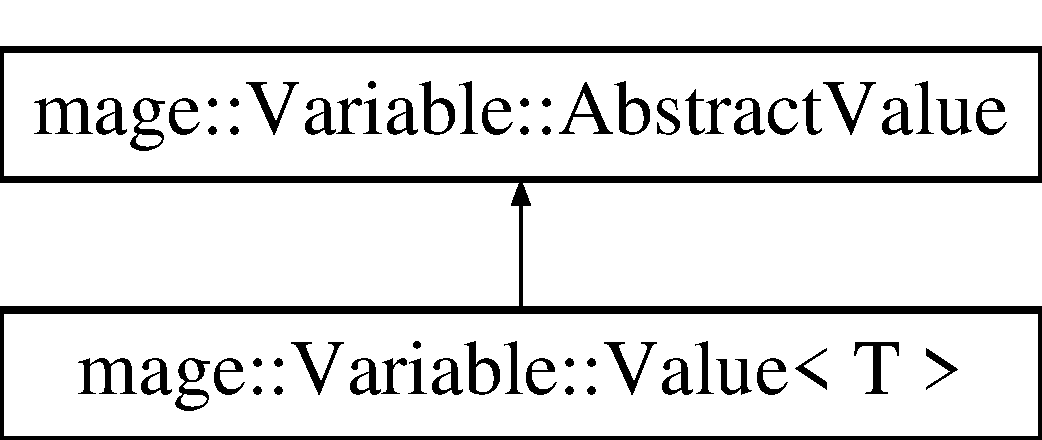
\includegraphics[height=2.000000cm]{structmage_1_1_variable_1_1_abstract_value}
\end{center}
\end{figure}
\subsection*{Public Member Functions}
\begin{DoxyCompactItemize}
\item 
virtual \hyperlink{structmage_1_1_variable_1_1_abstract_value_a7fa8fc14f81bb26f239af5f1263888a5}{$\sim$\+Abstract\+Value} ()=default
\item 
virtual const void $\ast$ \hyperlink{structmage_1_1_variable_1_1_abstract_value_aede2a77b571b80794a4254e34144f4c1}{Get\+Value} () const =0
\end{DoxyCompactItemize}
\subsection*{Protected Member Functions}
\begin{DoxyCompactItemize}
\item 
\hyperlink{structmage_1_1_variable_1_1_abstract_value_a0a96662d36697af8a17b88f6a2d8efca}{Abstract\+Value} ()=default
\item 
\hyperlink{structmage_1_1_variable_1_1_abstract_value_a09123ab568948a1a8bc7911c65fda422}{Abstract\+Value} (const \hyperlink{structmage_1_1_variable_1_1_abstract_value}{Abstract\+Value} \&abstract\+\_\+value)=default
\end{DoxyCompactItemize}
\subsection*{Private Member Functions}
\begin{DoxyCompactItemize}
\item 
\hyperlink{structmage_1_1_variable_1_1_abstract_value}{Abstract\+Value} \& \hyperlink{structmage_1_1_variable_1_1_abstract_value_a77f7107e78716a0ea76cfaedd0a50a4b}{operator=} (const \hyperlink{structmage_1_1_variable_1_1_abstract_value}{Abstract\+Value} \&abstract\+\_\+value)=delete
\end{DoxyCompactItemize}


\subsection{Detailed Description}
A struct of immutable abstract values.

\begin{DoxyNote}{Note}
This is an example of the Type Erasure pattern for templates. We need to keep the original type to ensure the right destructor can be called in case of non-\/primitive types. 
\end{DoxyNote}


\subsection{Constructor \& Destructor Documentation}
\hypertarget{structmage_1_1_variable_1_1_abstract_value_a7fa8fc14f81bb26f239af5f1263888a5}{}\label{structmage_1_1_variable_1_1_abstract_value_a7fa8fc14f81bb26f239af5f1263888a5} 
\index{mage\+::\+Variable\+::\+Abstract\+Value@{mage\+::\+Variable\+::\+Abstract\+Value}!````~Abstract\+Value@{$\sim$\+Abstract\+Value}}
\index{````~Abstract\+Value@{$\sim$\+Abstract\+Value}!mage\+::\+Variable\+::\+Abstract\+Value@{mage\+::\+Variable\+::\+Abstract\+Value}}
\subsubsection{\texorpdfstring{$\sim$\+Abstract\+Value()}{~AbstractValue()}}
{\footnotesize\ttfamily virtual mage\+::\+Variable\+::\+Abstract\+Value\+::$\sim$\+Abstract\+Value (\begin{DoxyParamCaption}{ }\end{DoxyParamCaption})\hspace{0.3cm}{\ttfamily [virtual]}, {\ttfamily [default]}}

Destructs this value. \hypertarget{structmage_1_1_variable_1_1_abstract_value_a0a96662d36697af8a17b88f6a2d8efca}{}\label{structmage_1_1_variable_1_1_abstract_value_a0a96662d36697af8a17b88f6a2d8efca} 
\index{mage\+::\+Variable\+::\+Abstract\+Value@{mage\+::\+Variable\+::\+Abstract\+Value}!Abstract\+Value@{Abstract\+Value}}
\index{Abstract\+Value@{Abstract\+Value}!mage\+::\+Variable\+::\+Abstract\+Value@{mage\+::\+Variable\+::\+Abstract\+Value}}
\subsubsection{\texorpdfstring{Abstract\+Value()}{AbstractValue()}\hspace{0.1cm}{\footnotesize\ttfamily [1/2]}}
{\footnotesize\ttfamily mage\+::\+Variable\+::\+Abstract\+Value\+::\+Abstract\+Value (\begin{DoxyParamCaption}{ }\end{DoxyParamCaption})\hspace{0.3cm}{\ttfamily [protected]}, {\ttfamily [default]}}

Constructs an abstract value. \hypertarget{structmage_1_1_variable_1_1_abstract_value_a09123ab568948a1a8bc7911c65fda422}{}\label{structmage_1_1_variable_1_1_abstract_value_a09123ab568948a1a8bc7911c65fda422} 
\index{mage\+::\+Variable\+::\+Abstract\+Value@{mage\+::\+Variable\+::\+Abstract\+Value}!Abstract\+Value@{Abstract\+Value}}
\index{Abstract\+Value@{Abstract\+Value}!mage\+::\+Variable\+::\+Abstract\+Value@{mage\+::\+Variable\+::\+Abstract\+Value}}
\subsubsection{\texorpdfstring{Abstract\+Value()}{AbstractValue()}\hspace{0.1cm}{\footnotesize\ttfamily [2/2]}}
{\footnotesize\ttfamily mage\+::\+Variable\+::\+Abstract\+Value\+::\+Abstract\+Value (\begin{DoxyParamCaption}\item[{const \hyperlink{structmage_1_1_variable_1_1_abstract_value}{Abstract\+Value} \&}]{abstract\+\_\+value }\end{DoxyParamCaption})\hspace{0.3cm}{\ttfamily [protected]}, {\ttfamily [default]}}

Constructs an abstract value from the given abstract value.


\begin{DoxyParams}[1]{Parameters}
\mbox{\tt in}  & {\em abstract\+\_\+value} & A reference to the abstract value. \\
\hline
\end{DoxyParams}


\subsection{Member Function Documentation}
\hypertarget{structmage_1_1_variable_1_1_abstract_value_aede2a77b571b80794a4254e34144f4c1}{}\label{structmage_1_1_variable_1_1_abstract_value_aede2a77b571b80794a4254e34144f4c1} 
\index{mage\+::\+Variable\+::\+Abstract\+Value@{mage\+::\+Variable\+::\+Abstract\+Value}!Get\+Value@{Get\+Value}}
\index{Get\+Value@{Get\+Value}!mage\+::\+Variable\+::\+Abstract\+Value@{mage\+::\+Variable\+::\+Abstract\+Value}}
\subsubsection{\texorpdfstring{Get\+Value()}{GetValue()}}
{\footnotesize\ttfamily virtual const void$\ast$ mage\+::\+Variable\+::\+Abstract\+Value\+::\+Get\+Value (\begin{DoxyParamCaption}{ }\end{DoxyParamCaption}) const\hspace{0.3cm}{\ttfamily [pure virtual]}}

Returns the value of this value.

\begin{DoxyReturn}{Returns}
A pointer to the value of this value. 
\end{DoxyReturn}


Implemented in \hyperlink{structmage_1_1_variable_1_1_value_a04d70496ebb7ad71dafa3df877daeb26}{mage\+::\+Variable\+::\+Value$<$ T $>$}.

\hypertarget{structmage_1_1_variable_1_1_abstract_value_a77f7107e78716a0ea76cfaedd0a50a4b}{}\label{structmage_1_1_variable_1_1_abstract_value_a77f7107e78716a0ea76cfaedd0a50a4b} 
\index{mage\+::\+Variable\+::\+Abstract\+Value@{mage\+::\+Variable\+::\+Abstract\+Value}!operator=@{operator=}}
\index{operator=@{operator=}!mage\+::\+Variable\+::\+Abstract\+Value@{mage\+::\+Variable\+::\+Abstract\+Value}}
\subsubsection{\texorpdfstring{operator=()}{operator=()}}
{\footnotesize\ttfamily \hyperlink{structmage_1_1_variable_1_1_abstract_value}{Abstract\+Value}\& mage\+::\+Variable\+::\+Abstract\+Value\+::operator= (\begin{DoxyParamCaption}\item[{const \hyperlink{structmage_1_1_variable_1_1_abstract_value}{Abstract\+Value} \&}]{abstract\+\_\+value }\end{DoxyParamCaption})\hspace{0.3cm}{\ttfamily [private]}, {\ttfamily [delete]}}

Copies the given abstract value to this abstract value.


\begin{DoxyParams}[1]{Parameters}
\mbox{\tt in}  & {\em abstract\+\_\+value} & A reference to the abstract value to copy from. \\
\hline
\end{DoxyParams}
\begin{DoxyReturn}{Returns}
A reference to the copy of the given abstract value (i.\+e. this abstract value). 
\end{DoxyReturn}

\hypertarget{structmage_1_1_b_s}{}\section{mage\+:\+:BS Struct Reference}
\label{structmage_1_1_b_s}\index{mage\+::\+BS@{mage\+::\+BS}}


{\ttfamily \#include $<$bounding\+\_\+volume.\+hpp$>$}

\subsection*{Public Member Functions}
\begin{DoxyCompactItemize}
\item 
\hyperlink{structmage_1_1_b_s_aa34921d9ea23b9a724ddf739b3adabfa}{BS} ()
\item 
\hyperlink{structmage_1_1_b_s_a23be36778ebc6b31fcfb31fb032fdb0e}{BS} (const \hyperlink{structmage_1_1_point3}{Point3} \&\hyperlink{structmage_1_1_b_s_a9c6ad8f37fa6b98179e8108c8584fdcf}{p}, float \hyperlink{structmage_1_1_b_s_ab2e786e8493feb28a3bc0216e8dea5bc}{r})
\item 
bool \hyperlink{structmage_1_1_b_s_a2ec64c652e8bf5417791958246d300cb}{Encloses} (const list$<$ X\+M\+F\+L\+O\+A\+T4 $>$ \&planes) const
\item 
bool \hyperlink{structmage_1_1_b_s_a6d9380b5a9a9aa59b7922b5be8e26e74}{Encloses\+Strict} (const list$<$ X\+M\+F\+L\+O\+A\+T4 $>$ \&planes) const
\item 
bool \hyperlink{structmage_1_1_b_s_a06f94772c3efd24c61cff33c018182f3}{Collides} (const \hyperlink{structmage_1_1_b_s}{BS} \&sphere, const X\+M\+F\+L\+O\+A\+T3 velocity\+\_\+sum, float $\ast$collision\+\_\+distance) const
\end{DoxyCompactItemize}
\subsection*{Public Attributes}
\begin{DoxyCompactItemize}
\item 
\hyperlink{structmage_1_1_point3}{Point3} \hyperlink{structmage_1_1_b_s_a9c6ad8f37fa6b98179e8108c8584fdcf}{p}
\item 
float \hyperlink{structmage_1_1_b_s_ab2e786e8493feb28a3bc0216e8dea5bc}{r}
\end{DoxyCompactItemize}


\subsection{Detailed Description}
A struct of Bounding Spheres (\hyperlink{structmage_1_1_b_s}{BS}). 

\subsection{Constructor \& Destructor Documentation}
\hypertarget{structmage_1_1_b_s_aa34921d9ea23b9a724ddf739b3adabfa}{}\label{structmage_1_1_b_s_aa34921d9ea23b9a724ddf739b3adabfa} 
\index{mage\+::\+BS@{mage\+::\+BS}!BS@{BS}}
\index{BS@{BS}!mage\+::\+BS@{mage\+::\+BS}}
\subsubsection{\texorpdfstring{B\+S()}{BS()}\hspace{0.1cm}{\footnotesize\ttfamily [1/2]}}
{\footnotesize\ttfamily mage\+::\+B\+S\+::\+BS (\begin{DoxyParamCaption}{ }\end{DoxyParamCaption})}

Constructs a sphere. \hypertarget{structmage_1_1_b_s_a23be36778ebc6b31fcfb31fb032fdb0e}{}\label{structmage_1_1_b_s_a23be36778ebc6b31fcfb31fb032fdb0e} 
\index{mage\+::\+BS@{mage\+::\+BS}!BS@{BS}}
\index{BS@{BS}!mage\+::\+BS@{mage\+::\+BS}}
\subsubsection{\texorpdfstring{B\+S()}{BS()}\hspace{0.1cm}{\footnotesize\ttfamily [2/2]}}
{\footnotesize\ttfamily mage\+::\+B\+S\+::\+BS (\begin{DoxyParamCaption}\item[{const \hyperlink{structmage_1_1_point3}{Point3} \&}]{p,  }\item[{float}]{r }\end{DoxyParamCaption})}

Constructs a sphere.


\begin{DoxyParams}[1]{Parameters}
\mbox{\tt in}  & {\em p} & The position \\
\hline
\mbox{\tt in}  & {\em r} & The radius. \\
\hline
\end{DoxyParams}


\subsection{Member Function Documentation}
\hypertarget{structmage_1_1_b_s_a06f94772c3efd24c61cff33c018182f3}{}\label{structmage_1_1_b_s_a06f94772c3efd24c61cff33c018182f3} 
\index{mage\+::\+BS@{mage\+::\+BS}!Collides@{Collides}}
\index{Collides@{Collides}!mage\+::\+BS@{mage\+::\+BS}}
\subsubsection{\texorpdfstring{Collides()}{Collides()}}
{\footnotesize\ttfamily bool mage\+::\+B\+S\+::\+Collides (\begin{DoxyParamCaption}\item[{const \hyperlink{structmage_1_1_b_s}{BS} \&}]{sphere,  }\item[{const X\+M\+F\+L\+O\+A\+T3}]{velocity\+\_\+sum,  }\item[{float $\ast$}]{collision\+\_\+distance }\end{DoxyParamCaption}) const}

Checks whether this sphere collides with a given sphere.


\begin{DoxyParams}[1]{Parameters}
\mbox{\tt in}  & {\em sphere} & The sphere. \\
\hline
\mbox{\tt in}  & {\em velocity\+\_\+sum} & The sum of the velocities of both spheres. \\
\hline
\mbox{\tt out}  & {\em collision\+\_\+distance} & The collision distance (in case of collision). \\
\hline
\end{DoxyParams}
\begin{DoxyReturn}{Returns}
{\ttfamily true} if this sphere collides with {\itshape sphere}. {\ttfamily false} otherwise. 
\end{DoxyReturn}
\hypertarget{structmage_1_1_b_s_a2ec64c652e8bf5417791958246d300cb}{}\label{structmage_1_1_b_s_a2ec64c652e8bf5417791958246d300cb} 
\index{mage\+::\+BS@{mage\+::\+BS}!Encloses@{Encloses}}
\index{Encloses@{Encloses}!mage\+::\+BS@{mage\+::\+BS}}
\subsubsection{\texorpdfstring{Encloses()}{Encloses()}}
{\footnotesize\ttfamily bool mage\+::\+B\+S\+::\+Encloses (\begin{DoxyParamCaption}\item[{const list$<$ X\+M\+F\+L\+O\+A\+T4 $>$ \&}]{planes }\end{DoxyParamCaption}) const}

Checks whether this sphere completely encloses the given (closed) volume.


\begin{DoxyParams}[1]{Parameters}
\mbox{\tt in}  & {\em planes} & A reference to a linked list containing the planes of the volume (each plane\textquotesingle{}s coefficients are represented as a {\ttfamily X\+M\+F\+L\+O\+A\+T4}). \\
\hline
\end{DoxyParams}
\begin{DoxyReturn}{Returns}
{\ttfamily true} if this sphere completely encloses {\itshape planes}. {\ttfamily false} otherwise. 
\end{DoxyReturn}
\hypertarget{structmage_1_1_b_s_a6d9380b5a9a9aa59b7922b5be8e26e74}{}\label{structmage_1_1_b_s_a6d9380b5a9a9aa59b7922b5be8e26e74} 
\index{mage\+::\+BS@{mage\+::\+BS}!Encloses\+Strict@{Encloses\+Strict}}
\index{Encloses\+Strict@{Encloses\+Strict}!mage\+::\+BS@{mage\+::\+BS}}
\subsubsection{\texorpdfstring{Encloses\+Strict()}{EnclosesStrict()}}
{\footnotesize\ttfamily bool mage\+::\+B\+S\+::\+Encloses\+Strict (\begin{DoxyParamCaption}\item[{const list$<$ X\+M\+F\+L\+O\+A\+T4 $>$ \&}]{planes }\end{DoxyParamCaption}) const}

Checks whether this sphere completely, strictly encloses the given (closed) volume.


\begin{DoxyParams}[1]{Parameters}
\mbox{\tt in}  & {\em planes} & A reference to a linked list containing the planes of the volume (each plane\textquotesingle{}s coefficients are represented as a {\ttfamily X\+M\+F\+L\+O\+A\+T4}). \\
\hline
\end{DoxyParams}
\begin{DoxyReturn}{Returns}
{\ttfamily true} if this sphere completely encloses {\itshape planes}. {\ttfamily false} otherwise. 
\end{DoxyReturn}


\subsection{Member Data Documentation}
\hypertarget{structmage_1_1_b_s_a9c6ad8f37fa6b98179e8108c8584fdcf}{}\label{structmage_1_1_b_s_a9c6ad8f37fa6b98179e8108c8584fdcf} 
\index{mage\+::\+BS@{mage\+::\+BS}!p@{p}}
\index{p@{p}!mage\+::\+BS@{mage\+::\+BS}}
\subsubsection{\texorpdfstring{p}{p}}
{\footnotesize\ttfamily \hyperlink{structmage_1_1_point3}{Point3} mage\+::\+B\+S\+::p}

The position of this sphere. \hypertarget{structmage_1_1_b_s_ab2e786e8493feb28a3bc0216e8dea5bc}{}\label{structmage_1_1_b_s_ab2e786e8493feb28a3bc0216e8dea5bc} 
\index{mage\+::\+BS@{mage\+::\+BS}!r@{r}}
\index{r@{r}!mage\+::\+BS@{mage\+::\+BS}}
\subsubsection{\texorpdfstring{r}{r}}
{\footnotesize\ttfamily float mage\+::\+B\+S\+::r}

The radius of this sphere. 
\hypertarget{classmage_1_1_camera}{}\section{mage\+:\+:Camera Class Reference}
\label{classmage_1_1_camera}\index{mage\+::\+Camera@{mage\+::\+Camera}}


{\ttfamily \#include $<$camera.\+hpp$>$}

Inheritance diagram for mage\+:\+:Camera\+:\begin{figure}[H]
\begin{center}
\leavevmode
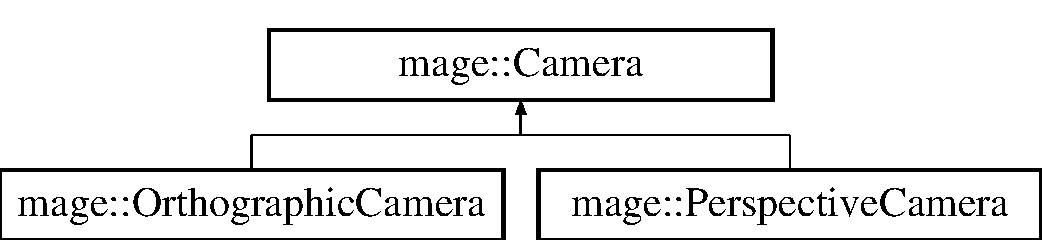
\includegraphics[height=2.000000cm]{classmage_1_1_camera}
\end{center}
\end{figure}
\subsection*{Public Member Functions}
\begin{DoxyCompactItemize}
\item 
virtual \hyperlink{classmage_1_1_camera_ae56c0542ae1a480c7fb15d737bf16de0}{$\sim$\+Camera} ()
\item 
\hyperlink{structmage_1_1_transform}{Transform} \& \hyperlink{classmage_1_1_camera_aaa5f4f2b5b13ffb1f70b77aec8579be5}{Get\+Transform} ()
\item 
const \hyperlink{structmage_1_1_transform}{Transform} \& \hyperlink{classmage_1_1_camera_adac4b7ef332babf36e0c9f271f1fff76}{Get\+Transform} () const
\item 
float \hyperlink{classmage_1_1_camera_a2285655605035118861297b2449a3443}{Get\+Width} () const
\item 
void \hyperlink{classmage_1_1_camera_aa99e2452c6d0629e7018d32cb9d222dd}{Set\+Width} (float width)
\item 
float \hyperlink{classmage_1_1_camera_a4c6c5e96085651ce29cd6e87543d21ec}{Get\+Height} () const
\item 
void \hyperlink{classmage_1_1_camera_a53ca727373580b145339d4dd93e2c65f}{Set\+Height} (float height)
\item 
void \hyperlink{classmage_1_1_camera_a637d09eeedc8015c661751f3b192e252}{Set\+Width\+And\+Height} (float width, float height)
\item 
float \hyperlink{classmage_1_1_camera_a175e3c36526a8a3e28cd2f8bd1701c55}{Get\+NearZ} () const
\item 
void \hyperlink{classmage_1_1_camera_a4aa60bcc75822457ccb8be2ff0ce93a4}{Set\+NearZ} (float near\+\_\+z)
\item 
float \hyperlink{classmage_1_1_camera_a7f293a8711086b3419fe3b4224ff2778}{Get\+FarZ} () const
\item 
void \hyperlink{classmage_1_1_camera_aaad9cb302d7ceb2515c2a23f094a6ce9}{Set\+FarZ} (float far\+\_\+z)
\item 
void \hyperlink{classmage_1_1_camera_a1800467939c0806405e9a708dbd838f8}{Set\+Near\+And\+FarZ} (float near\+\_\+z, float far\+\_\+z)
\item 
X\+M\+M\+A\+T\+R\+IX \hyperlink{classmage_1_1_camera_a4254e1c9d65c41b27842f35870fd7960}{Get\+View\+To\+Projection\+Matrix} () const
\end{DoxyCompactItemize}
\subsection*{Protected Member Functions}
\begin{DoxyCompactItemize}
\item 
\hyperlink{classmage_1_1_camera_a21ce33c0d4f4e3fb2cbbd9ba8d024a23}{Camera} (const X\+M\+M\+A\+T\+R\+IX \&view\+\_\+to\+\_\+projection, float width, float height, float near\+\_\+z=M\+A\+G\+E\+\_\+\+D\+E\+F\+A\+U\+L\+T\+\_\+\+C\+A\+M\+E\+R\+A\+\_\+\+N\+E\+A\+R\+\_\+Z, float far\+\_\+z=M\+A\+G\+E\+\_\+\+D\+E\+F\+A\+U\+L\+T\+\_\+\+C\+A\+M\+E\+R\+A\+\_\+\+F\+A\+R\+\_\+Z, const \hyperlink{structmage_1_1_transform}{Transform} \&transform=\hyperlink{structmage_1_1_transform}{Transform}())
\item 
virtual void \hyperlink{classmage_1_1_camera_a7f43b79d363e0c72b0bb42a06b65fb7e}{Update\+View\+To\+Projection\+Matrix} ()=0
\end{DoxyCompactItemize}
\subsection*{Protected Attributes}
\begin{DoxyCompactItemize}
\item 
\hyperlink{structmage_1_1_transform}{Transform} \hyperlink{classmage_1_1_camera_a5f7bd764e2a4a9221bf1f157fa23b3af}{m\+\_\+transform}
\item 
float \hyperlink{classmage_1_1_camera_acc8f371214af02fdac9a1ff04508c4ca}{m\+\_\+width}
\item 
float \hyperlink{classmage_1_1_camera_a48485eca596702f0e5985ec8b7db35a5}{m\+\_\+height}
\item 
float \hyperlink{classmage_1_1_camera_a685f8700a29d1f1eff2bec353c3ec970}{m\+\_\+near\+\_\+z}
\item 
float \hyperlink{classmage_1_1_camera_abe2eeca725ce3da238256007454b241f}{m\+\_\+far\+\_\+z}
\item 
X\+M\+M\+A\+T\+R\+IX \hyperlink{classmage_1_1_camera_a37b814e26a4c733a40a5f6fea691e958}{m\+\_\+view\+\_\+to\+\_\+projection}
\end{DoxyCompactItemize}


\subsection{Constructor \& Destructor Documentation}
\hypertarget{classmage_1_1_camera_ae56c0542ae1a480c7fb15d737bf16de0}{}\label{classmage_1_1_camera_ae56c0542ae1a480c7fb15d737bf16de0} 
\index{mage\+::\+Camera@{mage\+::\+Camera}!````~Camera@{$\sim$\+Camera}}
\index{````~Camera@{$\sim$\+Camera}!mage\+::\+Camera@{mage\+::\+Camera}}
\subsubsection{\texorpdfstring{$\sim$\+Camera()}{~Camera()}}
{\footnotesize\ttfamily virtual mage\+::\+Camera\+::$\sim$\+Camera (\begin{DoxyParamCaption}{ }\end{DoxyParamCaption})\hspace{0.3cm}{\ttfamily [virtual]}}

\hypertarget{classmage_1_1_camera_a21ce33c0d4f4e3fb2cbbd9ba8d024a23}{}\label{classmage_1_1_camera_a21ce33c0d4f4e3fb2cbbd9ba8d024a23} 
\index{mage\+::\+Camera@{mage\+::\+Camera}!Camera@{Camera}}
\index{Camera@{Camera}!mage\+::\+Camera@{mage\+::\+Camera}}
\subsubsection{\texorpdfstring{Camera()}{Camera()}}
{\footnotesize\ttfamily mage\+::\+Camera\+::\+Camera (\begin{DoxyParamCaption}\item[{const X\+M\+M\+A\+T\+R\+IX \&}]{view\+\_\+to\+\_\+projection,  }\item[{float}]{width,  }\item[{float}]{height,  }\item[{float}]{near\+\_\+z = {\ttfamily MAGE\+\_\+DEFAULT\+\_\+CAMERA\+\_\+NEAR\+\_\+Z},  }\item[{float}]{far\+\_\+z = {\ttfamily MAGE\+\_\+DEFAULT\+\_\+CAMERA\+\_\+FAR\+\_\+Z},  }\item[{const \hyperlink{structmage_1_1_transform}{Transform} \&}]{transform = {\ttfamily \hyperlink{structmage_1_1_transform}{Transform}()} }\end{DoxyParamCaption})\hspace{0.3cm}{\ttfamily [protected]}}



\subsection{Member Function Documentation}
\hypertarget{classmage_1_1_camera_a7f293a8711086b3419fe3b4224ff2778}{}\label{classmage_1_1_camera_a7f293a8711086b3419fe3b4224ff2778} 
\index{mage\+::\+Camera@{mage\+::\+Camera}!Get\+FarZ@{Get\+FarZ}}
\index{Get\+FarZ@{Get\+FarZ}!mage\+::\+Camera@{mage\+::\+Camera}}
\subsubsection{\texorpdfstring{Get\+Far\+Z()}{GetFarZ()}}
{\footnotesize\ttfamily float mage\+::\+Camera\+::\+Get\+FarZ (\begin{DoxyParamCaption}{ }\end{DoxyParamCaption}) const}

\hypertarget{classmage_1_1_camera_a4c6c5e96085651ce29cd6e87543d21ec}{}\label{classmage_1_1_camera_a4c6c5e96085651ce29cd6e87543d21ec} 
\index{mage\+::\+Camera@{mage\+::\+Camera}!Get\+Height@{Get\+Height}}
\index{Get\+Height@{Get\+Height}!mage\+::\+Camera@{mage\+::\+Camera}}
\subsubsection{\texorpdfstring{Get\+Height()}{GetHeight()}}
{\footnotesize\ttfamily float mage\+::\+Camera\+::\+Get\+Height (\begin{DoxyParamCaption}{ }\end{DoxyParamCaption}) const}

\hypertarget{classmage_1_1_camera_a175e3c36526a8a3e28cd2f8bd1701c55}{}\label{classmage_1_1_camera_a175e3c36526a8a3e28cd2f8bd1701c55} 
\index{mage\+::\+Camera@{mage\+::\+Camera}!Get\+NearZ@{Get\+NearZ}}
\index{Get\+NearZ@{Get\+NearZ}!mage\+::\+Camera@{mage\+::\+Camera}}
\subsubsection{\texorpdfstring{Get\+Near\+Z()}{GetNearZ()}}
{\footnotesize\ttfamily float mage\+::\+Camera\+::\+Get\+NearZ (\begin{DoxyParamCaption}{ }\end{DoxyParamCaption}) const}

\hypertarget{classmage_1_1_camera_aaa5f4f2b5b13ffb1f70b77aec8579be5}{}\label{classmage_1_1_camera_aaa5f4f2b5b13ffb1f70b77aec8579be5} 
\index{mage\+::\+Camera@{mage\+::\+Camera}!Get\+Transform@{Get\+Transform}}
\index{Get\+Transform@{Get\+Transform}!mage\+::\+Camera@{mage\+::\+Camera}}
\subsubsection{\texorpdfstring{Get\+Transform()}{GetTransform()}\hspace{0.1cm}{\footnotesize\ttfamily [1/2]}}
{\footnotesize\ttfamily \hyperlink{structmage_1_1_transform}{Transform}\& mage\+::\+Camera\+::\+Get\+Transform (\begin{DoxyParamCaption}{ }\end{DoxyParamCaption})}

\hypertarget{classmage_1_1_camera_adac4b7ef332babf36e0c9f271f1fff76}{}\label{classmage_1_1_camera_adac4b7ef332babf36e0c9f271f1fff76} 
\index{mage\+::\+Camera@{mage\+::\+Camera}!Get\+Transform@{Get\+Transform}}
\index{Get\+Transform@{Get\+Transform}!mage\+::\+Camera@{mage\+::\+Camera}}
\subsubsection{\texorpdfstring{Get\+Transform()}{GetTransform()}\hspace{0.1cm}{\footnotesize\ttfamily [2/2]}}
{\footnotesize\ttfamily const \hyperlink{structmage_1_1_transform}{Transform}\& mage\+::\+Camera\+::\+Get\+Transform (\begin{DoxyParamCaption}{ }\end{DoxyParamCaption}) const}

\hypertarget{classmage_1_1_camera_a4254e1c9d65c41b27842f35870fd7960}{}\label{classmage_1_1_camera_a4254e1c9d65c41b27842f35870fd7960} 
\index{mage\+::\+Camera@{mage\+::\+Camera}!Get\+View\+To\+Projection\+Matrix@{Get\+View\+To\+Projection\+Matrix}}
\index{Get\+View\+To\+Projection\+Matrix@{Get\+View\+To\+Projection\+Matrix}!mage\+::\+Camera@{mage\+::\+Camera}}
\subsubsection{\texorpdfstring{Get\+View\+To\+Projection\+Matrix()}{GetViewToProjectionMatrix()}}
{\footnotesize\ttfamily X\+M\+M\+A\+T\+R\+IX mage\+::\+Camera\+::\+Get\+View\+To\+Projection\+Matrix (\begin{DoxyParamCaption}{ }\end{DoxyParamCaption}) const}

\hypertarget{classmage_1_1_camera_a2285655605035118861297b2449a3443}{}\label{classmage_1_1_camera_a2285655605035118861297b2449a3443} 
\index{mage\+::\+Camera@{mage\+::\+Camera}!Get\+Width@{Get\+Width}}
\index{Get\+Width@{Get\+Width}!mage\+::\+Camera@{mage\+::\+Camera}}
\subsubsection{\texorpdfstring{Get\+Width()}{GetWidth()}}
{\footnotesize\ttfamily float mage\+::\+Camera\+::\+Get\+Width (\begin{DoxyParamCaption}{ }\end{DoxyParamCaption}) const}

\hypertarget{classmage_1_1_camera_aaad9cb302d7ceb2515c2a23f094a6ce9}{}\label{classmage_1_1_camera_aaad9cb302d7ceb2515c2a23f094a6ce9} 
\index{mage\+::\+Camera@{mage\+::\+Camera}!Set\+FarZ@{Set\+FarZ}}
\index{Set\+FarZ@{Set\+FarZ}!mage\+::\+Camera@{mage\+::\+Camera}}
\subsubsection{\texorpdfstring{Set\+Far\+Z()}{SetFarZ()}}
{\footnotesize\ttfamily void mage\+::\+Camera\+::\+Set\+FarZ (\begin{DoxyParamCaption}\item[{float}]{far\+\_\+z }\end{DoxyParamCaption})}

\hypertarget{classmage_1_1_camera_a53ca727373580b145339d4dd93e2c65f}{}\label{classmage_1_1_camera_a53ca727373580b145339d4dd93e2c65f} 
\index{mage\+::\+Camera@{mage\+::\+Camera}!Set\+Height@{Set\+Height}}
\index{Set\+Height@{Set\+Height}!mage\+::\+Camera@{mage\+::\+Camera}}
\subsubsection{\texorpdfstring{Set\+Height()}{SetHeight()}}
{\footnotesize\ttfamily void mage\+::\+Camera\+::\+Set\+Height (\begin{DoxyParamCaption}\item[{float}]{height }\end{DoxyParamCaption})}

\hypertarget{classmage_1_1_camera_a1800467939c0806405e9a708dbd838f8}{}\label{classmage_1_1_camera_a1800467939c0806405e9a708dbd838f8} 
\index{mage\+::\+Camera@{mage\+::\+Camera}!Set\+Near\+And\+FarZ@{Set\+Near\+And\+FarZ}}
\index{Set\+Near\+And\+FarZ@{Set\+Near\+And\+FarZ}!mage\+::\+Camera@{mage\+::\+Camera}}
\subsubsection{\texorpdfstring{Set\+Near\+And\+Far\+Z()}{SetNearAndFarZ()}}
{\footnotesize\ttfamily void mage\+::\+Camera\+::\+Set\+Near\+And\+FarZ (\begin{DoxyParamCaption}\item[{float}]{near\+\_\+z,  }\item[{float}]{far\+\_\+z }\end{DoxyParamCaption})}

\hypertarget{classmage_1_1_camera_a4aa60bcc75822457ccb8be2ff0ce93a4}{}\label{classmage_1_1_camera_a4aa60bcc75822457ccb8be2ff0ce93a4} 
\index{mage\+::\+Camera@{mage\+::\+Camera}!Set\+NearZ@{Set\+NearZ}}
\index{Set\+NearZ@{Set\+NearZ}!mage\+::\+Camera@{mage\+::\+Camera}}
\subsubsection{\texorpdfstring{Set\+Near\+Z()}{SetNearZ()}}
{\footnotesize\ttfamily void mage\+::\+Camera\+::\+Set\+NearZ (\begin{DoxyParamCaption}\item[{float}]{near\+\_\+z }\end{DoxyParamCaption})}

\hypertarget{classmage_1_1_camera_aa99e2452c6d0629e7018d32cb9d222dd}{}\label{classmage_1_1_camera_aa99e2452c6d0629e7018d32cb9d222dd} 
\index{mage\+::\+Camera@{mage\+::\+Camera}!Set\+Width@{Set\+Width}}
\index{Set\+Width@{Set\+Width}!mage\+::\+Camera@{mage\+::\+Camera}}
\subsubsection{\texorpdfstring{Set\+Width()}{SetWidth()}}
{\footnotesize\ttfamily void mage\+::\+Camera\+::\+Set\+Width (\begin{DoxyParamCaption}\item[{float}]{width }\end{DoxyParamCaption})}

\hypertarget{classmage_1_1_camera_a637d09eeedc8015c661751f3b192e252}{}\label{classmage_1_1_camera_a637d09eeedc8015c661751f3b192e252} 
\index{mage\+::\+Camera@{mage\+::\+Camera}!Set\+Width\+And\+Height@{Set\+Width\+And\+Height}}
\index{Set\+Width\+And\+Height@{Set\+Width\+And\+Height}!mage\+::\+Camera@{mage\+::\+Camera}}
\subsubsection{\texorpdfstring{Set\+Width\+And\+Height()}{SetWidthAndHeight()}}
{\footnotesize\ttfamily void mage\+::\+Camera\+::\+Set\+Width\+And\+Height (\begin{DoxyParamCaption}\item[{float}]{width,  }\item[{float}]{height }\end{DoxyParamCaption})}

\hypertarget{classmage_1_1_camera_a7f43b79d363e0c72b0bb42a06b65fb7e}{}\label{classmage_1_1_camera_a7f43b79d363e0c72b0bb42a06b65fb7e} 
\index{mage\+::\+Camera@{mage\+::\+Camera}!Update\+View\+To\+Projection\+Matrix@{Update\+View\+To\+Projection\+Matrix}}
\index{Update\+View\+To\+Projection\+Matrix@{Update\+View\+To\+Projection\+Matrix}!mage\+::\+Camera@{mage\+::\+Camera}}
\subsubsection{\texorpdfstring{Update\+View\+To\+Projection\+Matrix()}{UpdateViewToProjectionMatrix()}}
{\footnotesize\ttfamily virtual void mage\+::\+Camera\+::\+Update\+View\+To\+Projection\+Matrix (\begin{DoxyParamCaption}{ }\end{DoxyParamCaption})\hspace{0.3cm}{\ttfamily [protected]}, {\ttfamily [pure virtual]}}



Implemented in \hyperlink{classmage_1_1_perspective_camera_a7ae5681ec62be68e4517c0407a1349f6}{mage\+::\+Perspective\+Camera}, and \hyperlink{classmage_1_1_orthographic_camera_a8f1f2c4209b3126c92ecbe8d0e03c23e}{mage\+::\+Orthographic\+Camera}.



\subsection{Member Data Documentation}
\hypertarget{classmage_1_1_camera_abe2eeca725ce3da238256007454b241f}{}\label{classmage_1_1_camera_abe2eeca725ce3da238256007454b241f} 
\index{mage\+::\+Camera@{mage\+::\+Camera}!m\+\_\+far\+\_\+z@{m\+\_\+far\+\_\+z}}
\index{m\+\_\+far\+\_\+z@{m\+\_\+far\+\_\+z}!mage\+::\+Camera@{mage\+::\+Camera}}
\subsubsection{\texorpdfstring{m\+\_\+far\+\_\+z}{m\_far\_z}}
{\footnotesize\ttfamily float mage\+::\+Camera\+::m\+\_\+far\+\_\+z\hspace{0.3cm}{\ttfamily [protected]}}

\hypertarget{classmage_1_1_camera_a48485eca596702f0e5985ec8b7db35a5}{}\label{classmage_1_1_camera_a48485eca596702f0e5985ec8b7db35a5} 
\index{mage\+::\+Camera@{mage\+::\+Camera}!m\+\_\+height@{m\+\_\+height}}
\index{m\+\_\+height@{m\+\_\+height}!mage\+::\+Camera@{mage\+::\+Camera}}
\subsubsection{\texorpdfstring{m\+\_\+height}{m\_height}}
{\footnotesize\ttfamily float mage\+::\+Camera\+::m\+\_\+height\hspace{0.3cm}{\ttfamily [protected]}}

\hypertarget{classmage_1_1_camera_a685f8700a29d1f1eff2bec353c3ec970}{}\label{classmage_1_1_camera_a685f8700a29d1f1eff2bec353c3ec970} 
\index{mage\+::\+Camera@{mage\+::\+Camera}!m\+\_\+near\+\_\+z@{m\+\_\+near\+\_\+z}}
\index{m\+\_\+near\+\_\+z@{m\+\_\+near\+\_\+z}!mage\+::\+Camera@{mage\+::\+Camera}}
\subsubsection{\texorpdfstring{m\+\_\+near\+\_\+z}{m\_near\_z}}
{\footnotesize\ttfamily float mage\+::\+Camera\+::m\+\_\+near\+\_\+z\hspace{0.3cm}{\ttfamily [protected]}}

\hypertarget{classmage_1_1_camera_a5f7bd764e2a4a9221bf1f157fa23b3af}{}\label{classmage_1_1_camera_a5f7bd764e2a4a9221bf1f157fa23b3af} 
\index{mage\+::\+Camera@{mage\+::\+Camera}!m\+\_\+transform@{m\+\_\+transform}}
\index{m\+\_\+transform@{m\+\_\+transform}!mage\+::\+Camera@{mage\+::\+Camera}}
\subsubsection{\texorpdfstring{m\+\_\+transform}{m\_transform}}
{\footnotesize\ttfamily \hyperlink{structmage_1_1_transform}{Transform} mage\+::\+Camera\+::m\+\_\+transform\hspace{0.3cm}{\ttfamily [protected]}}

\hypertarget{classmage_1_1_camera_a37b814e26a4c733a40a5f6fea691e958}{}\label{classmage_1_1_camera_a37b814e26a4c733a40a5f6fea691e958} 
\index{mage\+::\+Camera@{mage\+::\+Camera}!m\+\_\+view\+\_\+to\+\_\+projection@{m\+\_\+view\+\_\+to\+\_\+projection}}
\index{m\+\_\+view\+\_\+to\+\_\+projection@{m\+\_\+view\+\_\+to\+\_\+projection}!mage\+::\+Camera@{mage\+::\+Camera}}
\subsubsection{\texorpdfstring{m\+\_\+view\+\_\+to\+\_\+projection}{m\_view\_to\_projection}}
{\footnotesize\ttfamily X\+M\+M\+A\+T\+R\+IX mage\+::\+Camera\+::m\+\_\+view\+\_\+to\+\_\+projection\hspace{0.3cm}{\ttfamily [protected]}}

\hypertarget{classmage_1_1_camera_acc8f371214af02fdac9a1ff04508c4ca}{}\label{classmage_1_1_camera_acc8f371214af02fdac9a1ff04508c4ca} 
\index{mage\+::\+Camera@{mage\+::\+Camera}!m\+\_\+width@{m\+\_\+width}}
\index{m\+\_\+width@{m\+\_\+width}!mage\+::\+Camera@{mage\+::\+Camera}}
\subsubsection{\texorpdfstring{m\+\_\+width}{m\_width}}
{\footnotesize\ttfamily float mage\+::\+Camera\+::m\+\_\+width\hspace{0.3cm}{\ttfamily [protected]}}


\hypertarget{classmage_1_1_camera_node}{}\section{mage\+:\+:Camera\+Node Class Reference}
\label{classmage_1_1_camera_node}\index{mage\+::\+Camera\+Node@{mage\+::\+Camera\+Node}}


{\ttfamily \#include $<$camera\+\_\+node.\+hpp$>$}

Inheritance diagram for mage\+:\+:Camera\+Node\+:\begin{figure}[H]
\begin{center}
\leavevmode
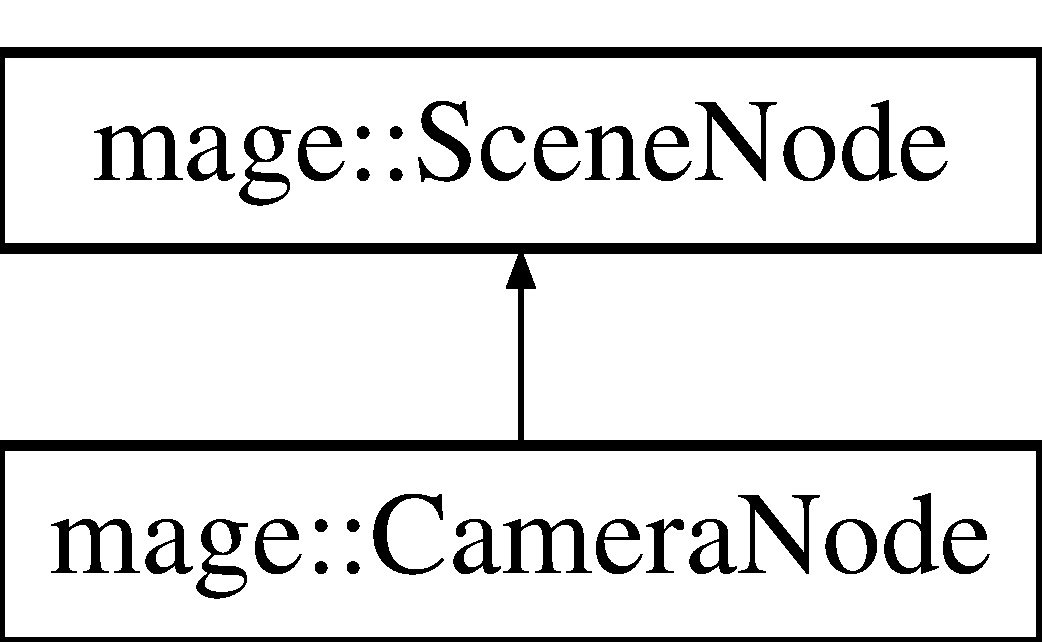
\includegraphics[height=2.000000cm]{classmage_1_1_camera_node}
\end{center}
\end{figure}
\subsection*{Public Member Functions}
\begin{DoxyCompactItemize}
\item 
\hyperlink{classmage_1_1_camera_node_aa6b469b939b268275665f5b962b82d4a}{Camera\+Node} (\hyperlink{classmage_1_1_camera}{Camera} $\ast$camera, const \hyperlink{structmage_1_1_transform}{Transform} \&transform=\hyperlink{structmage_1_1_transform}{Transform}())
\item 
virtual \hyperlink{classmage_1_1_camera_node_a2b66360b99bf03ee2f66a3a74be31792}{$\sim$\+Camera\+Node} ()
\item 
\hyperlink{classmage_1_1_camera}{Camera} $\ast$ \hyperlink{classmage_1_1_camera_node_a7cd05fd41271259870483de5b3ed6ebe}{Get\+Camera} () const
\item 
virtual void \hyperlink{classmage_1_1_camera_node_aed9c3c12cc4163fed880c49e43380efe}{Accept} (\hyperlink{classmage_1_1_scene_node_visitor}{Scene\+Node\+Visitor} \&visitor) override
\item 
virtual void \hyperlink{classmage_1_1_camera_node_a8b94f57b3a04f70b2c04a3d7c1ba3082}{Accept} (\hyperlink{classmage_1_1_scene_node_visitor}{Scene\+Node\+Visitor} \&visitor) const override
\end{DoxyCompactItemize}
\subsection*{Protected Attributes}
\begin{DoxyCompactItemize}
\item 
\hyperlink{classmage_1_1_camera}{Camera} $\ast$ \hyperlink{classmage_1_1_camera_node_aee902112c2e70e8de69b69aed303ca1f}{m\+\_\+camera}
\end{DoxyCompactItemize}
\subsection*{Additional Inherited Members}


\subsection{Detailed Description}
A class of camera nodes. 

\subsection{Constructor \& Destructor Documentation}
\hypertarget{classmage_1_1_camera_node_aa6b469b939b268275665f5b962b82d4a}{}\label{classmage_1_1_camera_node_aa6b469b939b268275665f5b962b82d4a} 
\index{mage\+::\+Camera\+Node@{mage\+::\+Camera\+Node}!Camera\+Node@{Camera\+Node}}
\index{Camera\+Node@{Camera\+Node}!mage\+::\+Camera\+Node@{mage\+::\+Camera\+Node}}
\subsubsection{\texorpdfstring{Camera\+Node()}{CameraNode()}}
{\footnotesize\ttfamily mage\+::\+Camera\+Node\+::\+Camera\+Node (\begin{DoxyParamCaption}\item[{\hyperlink{classmage_1_1_camera}{Camera} $\ast$}]{camera,  }\item[{const \hyperlink{structmage_1_1_transform}{Transform} \&}]{transform = {\ttfamily \hyperlink{structmage_1_1_transform}{Transform}()} }\end{DoxyParamCaption})}

Constructs a camera node with given camera and transform.

\begin{DoxyPrecond}{Precondition}
{\itshape camera} may not point to {\ttfamily nullptr}. 
\end{DoxyPrecond}

\begin{DoxyParams}[1]{Parameters}
\mbox{\tt in}  & {\em camera} & A pointer to the camera. \\
\hline
\mbox{\tt in}  & {\em transform} & A reference to the transform. \\
\hline
\end{DoxyParams}
\hypertarget{classmage_1_1_camera_node_a2b66360b99bf03ee2f66a3a74be31792}{}\label{classmage_1_1_camera_node_a2b66360b99bf03ee2f66a3a74be31792} 
\index{mage\+::\+Camera\+Node@{mage\+::\+Camera\+Node}!````~Camera\+Node@{$\sim$\+Camera\+Node}}
\index{````~Camera\+Node@{$\sim$\+Camera\+Node}!mage\+::\+Camera\+Node@{mage\+::\+Camera\+Node}}
\subsubsection{\texorpdfstring{$\sim$\+Camera\+Node()}{~CameraNode()}}
{\footnotesize\ttfamily virtual mage\+::\+Camera\+Node\+::$\sim$\+Camera\+Node (\begin{DoxyParamCaption}{ }\end{DoxyParamCaption})\hspace{0.3cm}{\ttfamily [virtual]}}

Destructs this camera node. 

\subsection{Member Function Documentation}
\hypertarget{classmage_1_1_camera_node_aed9c3c12cc4163fed880c49e43380efe}{}\label{classmage_1_1_camera_node_aed9c3c12cc4163fed880c49e43380efe} 
\index{mage\+::\+Camera\+Node@{mage\+::\+Camera\+Node}!Accept@{Accept}}
\index{Accept@{Accept}!mage\+::\+Camera\+Node@{mage\+::\+Camera\+Node}}
\subsubsection{\texorpdfstring{Accept()}{Accept()}\hspace{0.1cm}{\footnotesize\ttfamily [1/2]}}
{\footnotesize\ttfamily virtual void mage\+::\+Camera\+Node\+::\+Accept (\begin{DoxyParamCaption}\item[{\hyperlink{classmage_1_1_scene_node_visitor}{Scene\+Node\+Visitor} \&}]{visitor }\end{DoxyParamCaption})\hspace{0.3cm}{\ttfamily [override]}, {\ttfamily [virtual]}}

Accepts the given visitor.


\begin{DoxyParams}[1]{Parameters}
\mbox{\tt in}  & {\em visitor} & A reference to the visitor. \\
\hline
\end{DoxyParams}


Implements \hyperlink{classmage_1_1_scene_node_a32ed8763c8f8b4caa155f64551d96f13}{mage\+::\+Scene\+Node}.

\hypertarget{classmage_1_1_camera_node_a8b94f57b3a04f70b2c04a3d7c1ba3082}{}\label{classmage_1_1_camera_node_a8b94f57b3a04f70b2c04a3d7c1ba3082} 
\index{mage\+::\+Camera\+Node@{mage\+::\+Camera\+Node}!Accept@{Accept}}
\index{Accept@{Accept}!mage\+::\+Camera\+Node@{mage\+::\+Camera\+Node}}
\subsubsection{\texorpdfstring{Accept()}{Accept()}\hspace{0.1cm}{\footnotesize\ttfamily [2/2]}}
{\footnotesize\ttfamily virtual void mage\+::\+Camera\+Node\+::\+Accept (\begin{DoxyParamCaption}\item[{\hyperlink{classmage_1_1_scene_node_visitor}{Scene\+Node\+Visitor} \&}]{visitor }\end{DoxyParamCaption}) const\hspace{0.3cm}{\ttfamily [override]}, {\ttfamily [virtual]}}

Accepts the given visitor.


\begin{DoxyParams}[1]{Parameters}
\mbox{\tt in}  & {\em visitor} & A reference to the visitor. \\
\hline
\end{DoxyParams}


Implements \hyperlink{classmage_1_1_scene_node_a35fbfd49185fb61cb4e9edf56af35262}{mage\+::\+Scene\+Node}.

\hypertarget{classmage_1_1_camera_node_a7cd05fd41271259870483de5b3ed6ebe}{}\label{classmage_1_1_camera_node_a7cd05fd41271259870483de5b3ed6ebe} 
\index{mage\+::\+Camera\+Node@{mage\+::\+Camera\+Node}!Get\+Camera@{Get\+Camera}}
\index{Get\+Camera@{Get\+Camera}!mage\+::\+Camera\+Node@{mage\+::\+Camera\+Node}}
\subsubsection{\texorpdfstring{Get\+Camera()}{GetCamera()}}
{\footnotesize\ttfamily \hyperlink{classmage_1_1_camera}{Camera}$\ast$ mage\+::\+Camera\+Node\+::\+Get\+Camera (\begin{DoxyParamCaption}{ }\end{DoxyParamCaption}) const}

Returns the camera of this camera node.

\begin{DoxyReturn}{Returns}
A pointer to the camera of this camera node. 
\end{DoxyReturn}


\subsection{Member Data Documentation}
\hypertarget{classmage_1_1_camera_node_aee902112c2e70e8de69b69aed303ca1f}{}\label{classmage_1_1_camera_node_aee902112c2e70e8de69b69aed303ca1f} 
\index{mage\+::\+Camera\+Node@{mage\+::\+Camera\+Node}!m\+\_\+camera@{m\+\_\+camera}}
\index{m\+\_\+camera@{m\+\_\+camera}!mage\+::\+Camera\+Node@{mage\+::\+Camera\+Node}}
\subsubsection{\texorpdfstring{m\+\_\+camera}{m\_camera}}
{\footnotesize\ttfamily \hyperlink{classmage_1_1_camera}{Camera}$\ast$ mage\+::\+Camera\+Node\+::m\+\_\+camera\hspace{0.3cm}{\ttfamily [protected]}}

A pointer to the camera of this camera node. 
\hypertarget{structmage_1_1_cartesian_axes_system}{}\section{mage\+:\+:Cartesian\+Axes\+System Struct Reference}
\label{structmage_1_1_cartesian_axes_system}\index{mage\+::\+Cartesian\+Axes\+System@{mage\+::\+Cartesian\+Axes\+System}}


{\ttfamily \#include $<$coordinate\+\_\+system.\+hpp$>$}

\subsection*{Public Member Functions}
\begin{DoxyCompactItemize}
\item 
\hyperlink{structmage_1_1_cartesian_axes_system_a8f6ebcd50aafda44c478b7aa25e1fd25}{Cartesian\+Axes\+System} ()
\item 
\hyperlink{structmage_1_1_cartesian_axes_system_afd22b658e9221086add8c41958394568}{Cartesian\+Axes\+System} (const X\+M\+V\+E\+C\+T\+OR \&x)
\item 
\hyperlink{structmage_1_1_cartesian_axes_system_a8c5931061f227f6df8eec9ac8b9a7a18}{Cartesian\+Axes\+System} (const X\+M\+V\+E\+C\+T\+OR \&x, const X\+M\+V\+E\+C\+T\+OR \&y)
\item 
\hyperlink{structmage_1_1_cartesian_axes_system_a6d33ce6d7112d0cb63d93693036b986a}{Cartesian\+Axes\+System} (const X\+M\+V\+E\+C\+T\+OR \&x, const X\+M\+V\+E\+C\+T\+OR \&y, const X\+M\+V\+E\+C\+T\+OR \&z)
\item 
\hyperlink{structmage_1_1_cartesian_axes_system_a272ec4e772d87965617ba28957f5a558}{Cartesian\+Axes\+System} (const \hyperlink{structmage_1_1_cartesian_axes_system}{Cartesian\+Axes\+System} \&axes)=default
\item 
\hyperlink{structmage_1_1_cartesian_axes_system_a8c32f25e03757c03506d9a93bddf5d13}{$\sim$\+Cartesian\+Axes\+System} ()=default
\item 
\hyperlink{structmage_1_1_cartesian_axes_system}{Cartesian\+Axes\+System} \& \hyperlink{structmage_1_1_cartesian_axes_system_af52da9fbab85fc87921eff0ef6a17fe4}{operator=} (const \hyperlink{structmage_1_1_cartesian_axes_system}{Cartesian\+Axes\+System} \&axes)=default
\item 
X\+M\+V\+E\+C\+T\+OR \hyperlink{structmage_1_1_cartesian_axes_system_aa8e41490a0f9b333a8a9dde3a7544624}{Get\+AxisX} () const
\item 
X\+M\+V\+E\+C\+T\+OR \hyperlink{structmage_1_1_cartesian_axes_system_a1ab9d19fa733ce9667b244cd4a03b8fc}{Get\+AxisY} () const
\item 
X\+M\+V\+E\+C\+T\+OR \hyperlink{structmage_1_1_cartesian_axes_system_a143811599a089100b0327e719db44ec5}{Get\+AxisZ} () const
\end{DoxyCompactItemize}
\subsection*{Private Attributes}
\begin{DoxyCompactItemize}
\item 
X\+M\+V\+E\+C\+T\+OR \hyperlink{structmage_1_1_cartesian_axes_system_aa840c10ca92782e8c87c1ab53f0b86e9}{m\+\_\+x}
\item 
X\+M\+V\+E\+C\+T\+OR \hyperlink{structmage_1_1_cartesian_axes_system_a2cc6bc4fe185791a877e1418e85d6b47}{m\+\_\+y}
\item 
X\+M\+V\+E\+C\+T\+OR \hyperlink{structmage_1_1_cartesian_axes_system_abc733e5f82104391b0b352d263313d64}{m\+\_\+z}
\end{DoxyCompactItemize}


\subsection{Detailed Description}
A struct of Cartesian axes systems. 

\subsection{Constructor \& Destructor Documentation}
\hypertarget{structmage_1_1_cartesian_axes_system_a8f6ebcd50aafda44c478b7aa25e1fd25}{}\label{structmage_1_1_cartesian_axes_system_a8f6ebcd50aafda44c478b7aa25e1fd25} 
\index{mage\+::\+Cartesian\+Axes\+System@{mage\+::\+Cartesian\+Axes\+System}!Cartesian\+Axes\+System@{Cartesian\+Axes\+System}}
\index{Cartesian\+Axes\+System@{Cartesian\+Axes\+System}!mage\+::\+Cartesian\+Axes\+System@{mage\+::\+Cartesian\+Axes\+System}}
\subsubsection{\texorpdfstring{Cartesian\+Axes\+System()}{CartesianAxesSystem()}\hspace{0.1cm}{\footnotesize\ttfamily [1/5]}}
{\footnotesize\ttfamily mage\+::\+Cartesian\+Axes\+System\+::\+Cartesian\+Axes\+System (\begin{DoxyParamCaption}{ }\end{DoxyParamCaption})}

Constructs a Cartesian axes system. \hypertarget{structmage_1_1_cartesian_axes_system_afd22b658e9221086add8c41958394568}{}\label{structmage_1_1_cartesian_axes_system_afd22b658e9221086add8c41958394568} 
\index{mage\+::\+Cartesian\+Axes\+System@{mage\+::\+Cartesian\+Axes\+System}!Cartesian\+Axes\+System@{Cartesian\+Axes\+System}}
\index{Cartesian\+Axes\+System@{Cartesian\+Axes\+System}!mage\+::\+Cartesian\+Axes\+System@{mage\+::\+Cartesian\+Axes\+System}}
\subsubsection{\texorpdfstring{Cartesian\+Axes\+System()}{CartesianAxesSystem()}\hspace{0.1cm}{\footnotesize\ttfamily [2/5]}}
{\footnotesize\ttfamily mage\+::\+Cartesian\+Axes\+System\+::\+Cartesian\+Axes\+System (\begin{DoxyParamCaption}\item[{const X\+M\+V\+E\+C\+T\+OR \&}]{x }\end{DoxyParamCaption})}

Constructs a Cartesian axes system from the given axes.

\begin{DoxyPrecond}{Precondition}
The given axis is normalized. 
\end{DoxyPrecond}

\begin{DoxyParams}[1]{Parameters}
\mbox{\tt in}  & {\em x} & The x-\/axis. \\
\hline
\end{DoxyParams}
\hypertarget{structmage_1_1_cartesian_axes_system_a8c5931061f227f6df8eec9ac8b9a7a18}{}\label{structmage_1_1_cartesian_axes_system_a8c5931061f227f6df8eec9ac8b9a7a18} 
\index{mage\+::\+Cartesian\+Axes\+System@{mage\+::\+Cartesian\+Axes\+System}!Cartesian\+Axes\+System@{Cartesian\+Axes\+System}}
\index{Cartesian\+Axes\+System@{Cartesian\+Axes\+System}!mage\+::\+Cartesian\+Axes\+System@{mage\+::\+Cartesian\+Axes\+System}}
\subsubsection{\texorpdfstring{Cartesian\+Axes\+System()}{CartesianAxesSystem()}\hspace{0.1cm}{\footnotesize\ttfamily [3/5]}}
{\footnotesize\ttfamily mage\+::\+Cartesian\+Axes\+System\+::\+Cartesian\+Axes\+System (\begin{DoxyParamCaption}\item[{const X\+M\+V\+E\+C\+T\+OR \&}]{x,  }\item[{const X\+M\+V\+E\+C\+T\+OR \&}]{y }\end{DoxyParamCaption})}

Constructs a Cartesian axes system from the given axes.

\begin{DoxyPrecond}{Precondition}
The given axes are orthonormal. 
\end{DoxyPrecond}

\begin{DoxyParams}[1]{Parameters}
\mbox{\tt in}  & {\em x} & The x-\/axis. \\
\hline
\mbox{\tt in}  & {\em y} & The y-\/axis. \\
\hline
\end{DoxyParams}
\hypertarget{structmage_1_1_cartesian_axes_system_a6d33ce6d7112d0cb63d93693036b986a}{}\label{structmage_1_1_cartesian_axes_system_a6d33ce6d7112d0cb63d93693036b986a} 
\index{mage\+::\+Cartesian\+Axes\+System@{mage\+::\+Cartesian\+Axes\+System}!Cartesian\+Axes\+System@{Cartesian\+Axes\+System}}
\index{Cartesian\+Axes\+System@{Cartesian\+Axes\+System}!mage\+::\+Cartesian\+Axes\+System@{mage\+::\+Cartesian\+Axes\+System}}
\subsubsection{\texorpdfstring{Cartesian\+Axes\+System()}{CartesianAxesSystem()}\hspace{0.1cm}{\footnotesize\ttfamily [4/5]}}
{\footnotesize\ttfamily mage\+::\+Cartesian\+Axes\+System\+::\+Cartesian\+Axes\+System (\begin{DoxyParamCaption}\item[{const X\+M\+V\+E\+C\+T\+OR \&}]{x,  }\item[{const X\+M\+V\+E\+C\+T\+OR \&}]{y,  }\item[{const X\+M\+V\+E\+C\+T\+OR \&}]{z }\end{DoxyParamCaption})}

Constructs a Cartesian axes system from the given axes.

\begin{DoxyPrecond}{Precondition}
The given axes are orthonormal. 
\end{DoxyPrecond}

\begin{DoxyParams}[1]{Parameters}
\mbox{\tt in}  & {\em x} & The x-\/axis. \\
\hline
\mbox{\tt in}  & {\em y} & The y-\/axis. \\
\hline
\mbox{\tt in}  & {\em z} & The z-\/axis. \\
\hline
\end{DoxyParams}
\hypertarget{structmage_1_1_cartesian_axes_system_a272ec4e772d87965617ba28957f5a558}{}\label{structmage_1_1_cartesian_axes_system_a272ec4e772d87965617ba28957f5a558} 
\index{mage\+::\+Cartesian\+Axes\+System@{mage\+::\+Cartesian\+Axes\+System}!Cartesian\+Axes\+System@{Cartesian\+Axes\+System}}
\index{Cartesian\+Axes\+System@{Cartesian\+Axes\+System}!mage\+::\+Cartesian\+Axes\+System@{mage\+::\+Cartesian\+Axes\+System}}
\subsubsection{\texorpdfstring{Cartesian\+Axes\+System()}{CartesianAxesSystem()}\hspace{0.1cm}{\footnotesize\ttfamily [5/5]}}
{\footnotesize\ttfamily mage\+::\+Cartesian\+Axes\+System\+::\+Cartesian\+Axes\+System (\begin{DoxyParamCaption}\item[{const \hyperlink{structmage_1_1_cartesian_axes_system}{Cartesian\+Axes\+System} \&}]{axes }\end{DoxyParamCaption})\hspace{0.3cm}{\ttfamily [default]}}

Constructs a Cartesian axes system from the given Cartesian axes system.


\begin{DoxyParams}[1]{Parameters}
\mbox{\tt in}  & {\em axes} & The Cartesian axes system. \\
\hline
\end{DoxyParams}
\hypertarget{structmage_1_1_cartesian_axes_system_a8c32f25e03757c03506d9a93bddf5d13}{}\label{structmage_1_1_cartesian_axes_system_a8c32f25e03757c03506d9a93bddf5d13} 
\index{mage\+::\+Cartesian\+Axes\+System@{mage\+::\+Cartesian\+Axes\+System}!````~Cartesian\+Axes\+System@{$\sim$\+Cartesian\+Axes\+System}}
\index{````~Cartesian\+Axes\+System@{$\sim$\+Cartesian\+Axes\+System}!mage\+::\+Cartesian\+Axes\+System@{mage\+::\+Cartesian\+Axes\+System}}
\subsubsection{\texorpdfstring{$\sim$\+Cartesian\+Axes\+System()}{~CartesianAxesSystem()}}
{\footnotesize\ttfamily mage\+::\+Cartesian\+Axes\+System\+::$\sim$\+Cartesian\+Axes\+System (\begin{DoxyParamCaption}{ }\end{DoxyParamCaption})\hspace{0.3cm}{\ttfamily [default]}}

Destructs this Cartesian axes system. 

\subsection{Member Function Documentation}
\hypertarget{structmage_1_1_cartesian_axes_system_aa8e41490a0f9b333a8a9dde3a7544624}{}\label{structmage_1_1_cartesian_axes_system_aa8e41490a0f9b333a8a9dde3a7544624} 
\index{mage\+::\+Cartesian\+Axes\+System@{mage\+::\+Cartesian\+Axes\+System}!Get\+AxisX@{Get\+AxisX}}
\index{Get\+AxisX@{Get\+AxisX}!mage\+::\+Cartesian\+Axes\+System@{mage\+::\+Cartesian\+Axes\+System}}
\subsubsection{\texorpdfstring{Get\+Axis\+X()}{GetAxisX()}}
{\footnotesize\ttfamily X\+M\+V\+E\+C\+T\+OR mage\+::\+Cartesian\+Axes\+System\+::\+Get\+AxisX (\begin{DoxyParamCaption}{ }\end{DoxyParamCaption}) const}

Returns the x-\/axis of this Cartesian axes system.

\begin{DoxyReturn}{Returns}
The x-\/axis of this Cartesian axes system. 
\end{DoxyReturn}
\hypertarget{structmage_1_1_cartesian_axes_system_a1ab9d19fa733ce9667b244cd4a03b8fc}{}\label{structmage_1_1_cartesian_axes_system_a1ab9d19fa733ce9667b244cd4a03b8fc} 
\index{mage\+::\+Cartesian\+Axes\+System@{mage\+::\+Cartesian\+Axes\+System}!Get\+AxisY@{Get\+AxisY}}
\index{Get\+AxisY@{Get\+AxisY}!mage\+::\+Cartesian\+Axes\+System@{mage\+::\+Cartesian\+Axes\+System}}
\subsubsection{\texorpdfstring{Get\+Axis\+Y()}{GetAxisY()}}
{\footnotesize\ttfamily X\+M\+V\+E\+C\+T\+OR mage\+::\+Cartesian\+Axes\+System\+::\+Get\+AxisY (\begin{DoxyParamCaption}{ }\end{DoxyParamCaption}) const}

Returns the y-\/axis of this Cartesian axes system.

\begin{DoxyReturn}{Returns}
The y-\/axis of this Cartesian axes system. 
\end{DoxyReturn}
\hypertarget{structmage_1_1_cartesian_axes_system_a143811599a089100b0327e719db44ec5}{}\label{structmage_1_1_cartesian_axes_system_a143811599a089100b0327e719db44ec5} 
\index{mage\+::\+Cartesian\+Axes\+System@{mage\+::\+Cartesian\+Axes\+System}!Get\+AxisZ@{Get\+AxisZ}}
\index{Get\+AxisZ@{Get\+AxisZ}!mage\+::\+Cartesian\+Axes\+System@{mage\+::\+Cartesian\+Axes\+System}}
\subsubsection{\texorpdfstring{Get\+Axis\+Z()}{GetAxisZ()}}
{\footnotesize\ttfamily X\+M\+V\+E\+C\+T\+OR mage\+::\+Cartesian\+Axes\+System\+::\+Get\+AxisZ (\begin{DoxyParamCaption}{ }\end{DoxyParamCaption}) const}

Returns the z-\/axis of this Cartesian axes system.

\begin{DoxyReturn}{Returns}
The z-\/axis of this Cartesian axes system. 
\end{DoxyReturn}
\hypertarget{structmage_1_1_cartesian_axes_system_af52da9fbab85fc87921eff0ef6a17fe4}{}\label{structmage_1_1_cartesian_axes_system_af52da9fbab85fc87921eff0ef6a17fe4} 
\index{mage\+::\+Cartesian\+Axes\+System@{mage\+::\+Cartesian\+Axes\+System}!operator=@{operator=}}
\index{operator=@{operator=}!mage\+::\+Cartesian\+Axes\+System@{mage\+::\+Cartesian\+Axes\+System}}
\subsubsection{\texorpdfstring{operator=()}{operator=()}}
{\footnotesize\ttfamily \hyperlink{structmage_1_1_cartesian_axes_system}{Cartesian\+Axes\+System}\& mage\+::\+Cartesian\+Axes\+System\+::operator= (\begin{DoxyParamCaption}\item[{const \hyperlink{structmage_1_1_cartesian_axes_system}{Cartesian\+Axes\+System} \&}]{axes }\end{DoxyParamCaption})\hspace{0.3cm}{\ttfamily [default]}}

Copies the given Cartesian axes system to this Cartesian axes system.


\begin{DoxyParams}[1]{Parameters}
\mbox{\tt in}  & {\em axes} & The Cartesian axes system to copy from. \\
\hline
\end{DoxyParams}
\begin{DoxyReturn}{Returns}
A reference to the copy of the given Cartesian axes system (i.\+e. this Cartesian axes system). 
\end{DoxyReturn}


\subsection{Member Data Documentation}
\hypertarget{structmage_1_1_cartesian_axes_system_aa840c10ca92782e8c87c1ab53f0b86e9}{}\label{structmage_1_1_cartesian_axes_system_aa840c10ca92782e8c87c1ab53f0b86e9} 
\index{mage\+::\+Cartesian\+Axes\+System@{mage\+::\+Cartesian\+Axes\+System}!m\+\_\+x@{m\+\_\+x}}
\index{m\+\_\+x@{m\+\_\+x}!mage\+::\+Cartesian\+Axes\+System@{mage\+::\+Cartesian\+Axes\+System}}
\subsubsection{\texorpdfstring{m\+\_\+x}{m\_x}}
{\footnotesize\ttfamily X\+M\+V\+E\+C\+T\+OR mage\+::\+Cartesian\+Axes\+System\+::m\+\_\+x\hspace{0.3cm}{\ttfamily [private]}}

The x-\/axis of this Cartesian axes system. \hypertarget{structmage_1_1_cartesian_axes_system_a2cc6bc4fe185791a877e1418e85d6b47}{}\label{structmage_1_1_cartesian_axes_system_a2cc6bc4fe185791a877e1418e85d6b47} 
\index{mage\+::\+Cartesian\+Axes\+System@{mage\+::\+Cartesian\+Axes\+System}!m\+\_\+y@{m\+\_\+y}}
\index{m\+\_\+y@{m\+\_\+y}!mage\+::\+Cartesian\+Axes\+System@{mage\+::\+Cartesian\+Axes\+System}}
\subsubsection{\texorpdfstring{m\+\_\+y}{m\_y}}
{\footnotesize\ttfamily X\+M\+V\+E\+C\+T\+OR mage\+::\+Cartesian\+Axes\+System\+::m\+\_\+y\hspace{0.3cm}{\ttfamily [private]}}

The y-\/axis of this Cartesian axes system. \hypertarget{structmage_1_1_cartesian_axes_system_abc733e5f82104391b0b352d263313d64}{}\label{structmage_1_1_cartesian_axes_system_abc733e5f82104391b0b352d263313d64} 
\index{mage\+::\+Cartesian\+Axes\+System@{mage\+::\+Cartesian\+Axes\+System}!m\+\_\+z@{m\+\_\+z}}
\index{m\+\_\+z@{m\+\_\+z}!mage\+::\+Cartesian\+Axes\+System@{mage\+::\+Cartesian\+Axes\+System}}
\subsubsection{\texorpdfstring{m\+\_\+z}{m\_z}}
{\footnotesize\ttfamily X\+M\+V\+E\+C\+T\+OR mage\+::\+Cartesian\+Axes\+System\+::m\+\_\+z\hspace{0.3cm}{\ttfamily [private]}}

The z-\/axis of this Cartesian axes system. 
\hypertarget{structmage_1_1_cartesian_coordinate_system}{}\section{mage\+:\+:Cartesian\+Coordinate\+System Struct Reference}
\label{structmage_1_1_cartesian_coordinate_system}\index{mage\+::\+Cartesian\+Coordinate\+System@{mage\+::\+Cartesian\+Coordinate\+System}}


{\ttfamily \#include $<$coordinate\+\_\+system.\+hpp$>$}

\subsection*{Public Member Functions}
\begin{DoxyCompactItemize}
\item 
\hyperlink{structmage_1_1_cartesian_coordinate_system_a3f4a3309daccc818f06400a44f70b09b}{Cartesian\+Coordinate\+System} (const \hyperlink{structmage_1_1_cartesian_axes_system}{Cartesian\+Axes\+System} \&axes)
\item 
\hyperlink{structmage_1_1_cartesian_coordinate_system_a322dc634c9192c1d1f3f4872e6255b91}{Cartesian\+Coordinate\+System} (const X\+M\+V\+E\+C\+T\+OR \&o, const \hyperlink{structmage_1_1_cartesian_axes_system}{Cartesian\+Axes\+System} \&axes)
\item 
\hyperlink{structmage_1_1_cartesian_coordinate_system_a9243a8a56c11edca91e6287aa6cafeee}{Cartesian\+Coordinate\+System} (const \hyperlink{structmage_1_1_cartesian_coordinate_system}{Cartesian\+Coordinate\+System} \&coordinate\+\_\+system)
\item 
\hyperlink{structmage_1_1_cartesian_coordinate_system_a67ddbe028549f726db16066999c2c7c5}{$\sim$\+Cartesian\+Coordinate\+System} ()
\item 
\hyperlink{structmage_1_1_cartesian_coordinate_system}{Cartesian\+Coordinate\+System} \& \hyperlink{structmage_1_1_cartesian_coordinate_system_a4f11e67acce6eaa646e907bc6b485adf}{operator=} (const \hyperlink{structmage_1_1_cartesian_coordinate_system}{Cartesian\+Coordinate\+System} \&coordinate\+\_\+system)
\item 
X\+M\+V\+E\+C\+T\+OR \hyperlink{structmage_1_1_cartesian_coordinate_system_ac413d8f94f94102faa47d7c5cf8813b9}{Get\+Origin} () const
\item 
X\+M\+V\+E\+C\+T\+OR \hyperlink{structmage_1_1_cartesian_coordinate_system_ad79c4e6ae091d2a0268f1b9c1f06b7b2}{Get\+AxisX} () const
\item 
X\+M\+V\+E\+C\+T\+OR \hyperlink{structmage_1_1_cartesian_coordinate_system_a793c9783db21865ccf55f153cca963f3}{Get\+AxisY} () const
\item 
X\+M\+V\+E\+C\+T\+OR \hyperlink{structmage_1_1_cartesian_coordinate_system_ac152628841e8a51092b785bf62a64d98}{Get\+AxisZ} () const
\item 
\hyperlink{structmage_1_1_cartesian_axes_system}{Cartesian\+Axes\+System} \hyperlink{structmage_1_1_cartesian_coordinate_system_a291ba9d21e78af511bdd6358b3502eb4}{Get\+Axes} () const
\end{DoxyCompactItemize}
\subsection*{Private Attributes}
\begin{DoxyCompactItemize}
\item 
X\+M\+V\+E\+C\+T\+OR \hyperlink{structmage_1_1_cartesian_coordinate_system_a1ea373bb91be991ee221a2ce1e02be2b}{m\+\_\+o}
\item 
\hyperlink{structmage_1_1_cartesian_axes_system}{Cartesian\+Axes\+System} \hyperlink{structmage_1_1_cartesian_coordinate_system_acf7b8cf35026f5fa8fc11a126b96b055}{m\+\_\+axes}
\end{DoxyCompactItemize}


\subsection{Detailed Description}
A struct of Cartesian coordinate systems. 

\subsection{Constructor \& Destructor Documentation}
\hypertarget{structmage_1_1_cartesian_coordinate_system_a3f4a3309daccc818f06400a44f70b09b}{}\label{structmage_1_1_cartesian_coordinate_system_a3f4a3309daccc818f06400a44f70b09b} 
\index{mage\+::\+Cartesian\+Coordinate\+System@{mage\+::\+Cartesian\+Coordinate\+System}!Cartesian\+Coordinate\+System@{Cartesian\+Coordinate\+System}}
\index{Cartesian\+Coordinate\+System@{Cartesian\+Coordinate\+System}!mage\+::\+Cartesian\+Coordinate\+System@{mage\+::\+Cartesian\+Coordinate\+System}}
\subsubsection{\texorpdfstring{Cartesian\+Coordinate\+System()}{CartesianCoordinateSystem()}\hspace{0.1cm}{\footnotesize\ttfamily [1/3]}}
{\footnotesize\ttfamily mage\+::\+Cartesian\+Coordinate\+System\+::\+Cartesian\+Coordinate\+System (\begin{DoxyParamCaption}\item[{const \hyperlink{structmage_1_1_cartesian_axes_system}{Cartesian\+Axes\+System} \&}]{axes }\end{DoxyParamCaption})\hspace{0.3cm}{\ttfamily [explicit]}}

Constructs a Cartesian coordinate system from the given Cartesian axes system.


\begin{DoxyParams}[1]{Parameters}
\mbox{\tt in}  & {\em axes} & The Cartesian axes system. \\
\hline
\end{DoxyParams}
\hypertarget{structmage_1_1_cartesian_coordinate_system_a322dc634c9192c1d1f3f4872e6255b91}{}\label{structmage_1_1_cartesian_coordinate_system_a322dc634c9192c1d1f3f4872e6255b91} 
\index{mage\+::\+Cartesian\+Coordinate\+System@{mage\+::\+Cartesian\+Coordinate\+System}!Cartesian\+Coordinate\+System@{Cartesian\+Coordinate\+System}}
\index{Cartesian\+Coordinate\+System@{Cartesian\+Coordinate\+System}!mage\+::\+Cartesian\+Coordinate\+System@{mage\+::\+Cartesian\+Coordinate\+System}}
\subsubsection{\texorpdfstring{Cartesian\+Coordinate\+System()}{CartesianCoordinateSystem()}\hspace{0.1cm}{\footnotesize\ttfamily [2/3]}}
{\footnotesize\ttfamily mage\+::\+Cartesian\+Coordinate\+System\+::\+Cartesian\+Coordinate\+System (\begin{DoxyParamCaption}\item[{const X\+M\+V\+E\+C\+T\+OR \&}]{o,  }\item[{const \hyperlink{structmage_1_1_cartesian_axes_system}{Cartesian\+Axes\+System} \&}]{axes }\end{DoxyParamCaption})}

Constructs a Cartesian coordinate system from the given origin and Cartesian axes system.


\begin{DoxyParams}[1]{Parameters}
\mbox{\tt in}  & {\em o} & The origin. \\
\hline
\mbox{\tt in}  & {\em axes} & The Cartesian axes system. \\
\hline
\end{DoxyParams}
\hypertarget{structmage_1_1_cartesian_coordinate_system_a9243a8a56c11edca91e6287aa6cafeee}{}\label{structmage_1_1_cartesian_coordinate_system_a9243a8a56c11edca91e6287aa6cafeee} 
\index{mage\+::\+Cartesian\+Coordinate\+System@{mage\+::\+Cartesian\+Coordinate\+System}!Cartesian\+Coordinate\+System@{Cartesian\+Coordinate\+System}}
\index{Cartesian\+Coordinate\+System@{Cartesian\+Coordinate\+System}!mage\+::\+Cartesian\+Coordinate\+System@{mage\+::\+Cartesian\+Coordinate\+System}}
\subsubsection{\texorpdfstring{Cartesian\+Coordinate\+System()}{CartesianCoordinateSystem()}\hspace{0.1cm}{\footnotesize\ttfamily [3/3]}}
{\footnotesize\ttfamily mage\+::\+Cartesian\+Coordinate\+System\+::\+Cartesian\+Coordinate\+System (\begin{DoxyParamCaption}\item[{const \hyperlink{structmage_1_1_cartesian_coordinate_system}{Cartesian\+Coordinate\+System} \&}]{coordinate\+\_\+system }\end{DoxyParamCaption})}

Constructs a Cartesian coordinate system from the given Cartesian coordinate system.


\begin{DoxyParams}[1]{Parameters}
\mbox{\tt in}  & {\em coordinate\+\_\+system} & The Cartesian coordinate system. \\
\hline
\end{DoxyParams}
\hypertarget{structmage_1_1_cartesian_coordinate_system_a67ddbe028549f726db16066999c2c7c5}{}\label{structmage_1_1_cartesian_coordinate_system_a67ddbe028549f726db16066999c2c7c5} 
\index{mage\+::\+Cartesian\+Coordinate\+System@{mage\+::\+Cartesian\+Coordinate\+System}!````~Cartesian\+Coordinate\+System@{$\sim$\+Cartesian\+Coordinate\+System}}
\index{````~Cartesian\+Coordinate\+System@{$\sim$\+Cartesian\+Coordinate\+System}!mage\+::\+Cartesian\+Coordinate\+System@{mage\+::\+Cartesian\+Coordinate\+System}}
\subsubsection{\texorpdfstring{$\sim$\+Cartesian\+Coordinate\+System()}{~CartesianCoordinateSystem()}}
{\footnotesize\ttfamily mage\+::\+Cartesian\+Coordinate\+System\+::$\sim$\+Cartesian\+Coordinate\+System (\begin{DoxyParamCaption}{ }\end{DoxyParamCaption})}

Destructs this Cartesian coordinate system. 

\subsection{Member Function Documentation}
\hypertarget{structmage_1_1_cartesian_coordinate_system_a291ba9d21e78af511bdd6358b3502eb4}{}\label{structmage_1_1_cartesian_coordinate_system_a291ba9d21e78af511bdd6358b3502eb4} 
\index{mage\+::\+Cartesian\+Coordinate\+System@{mage\+::\+Cartesian\+Coordinate\+System}!Get\+Axes@{Get\+Axes}}
\index{Get\+Axes@{Get\+Axes}!mage\+::\+Cartesian\+Coordinate\+System@{mage\+::\+Cartesian\+Coordinate\+System}}
\subsubsection{\texorpdfstring{Get\+Axes()}{GetAxes()}}
{\footnotesize\ttfamily \hyperlink{structmage_1_1_cartesian_axes_system}{Cartesian\+Axes\+System} mage\+::\+Cartesian\+Coordinate\+System\+::\+Get\+Axes (\begin{DoxyParamCaption}{ }\end{DoxyParamCaption}) const}

Returns the axes of this Cartesian coordinate system.

\begin{DoxyReturn}{Returns}
The Cartesian axes system of this Cartesian coordinate system. 
\end{DoxyReturn}
\hypertarget{structmage_1_1_cartesian_coordinate_system_ad79c4e6ae091d2a0268f1b9c1f06b7b2}{}\label{structmage_1_1_cartesian_coordinate_system_ad79c4e6ae091d2a0268f1b9c1f06b7b2} 
\index{mage\+::\+Cartesian\+Coordinate\+System@{mage\+::\+Cartesian\+Coordinate\+System}!Get\+AxisX@{Get\+AxisX}}
\index{Get\+AxisX@{Get\+AxisX}!mage\+::\+Cartesian\+Coordinate\+System@{mage\+::\+Cartesian\+Coordinate\+System}}
\subsubsection{\texorpdfstring{Get\+Axis\+X()}{GetAxisX()}}
{\footnotesize\ttfamily X\+M\+V\+E\+C\+T\+OR mage\+::\+Cartesian\+Coordinate\+System\+::\+Get\+AxisX (\begin{DoxyParamCaption}{ }\end{DoxyParamCaption}) const}

Returns the x-\/axis of this Cartesian coordinate system.

\begin{DoxyReturn}{Returns}
The x-\/axis of this Cartesian coordinate system. 
\end{DoxyReturn}
\hypertarget{structmage_1_1_cartesian_coordinate_system_a793c9783db21865ccf55f153cca963f3}{}\label{structmage_1_1_cartesian_coordinate_system_a793c9783db21865ccf55f153cca963f3} 
\index{mage\+::\+Cartesian\+Coordinate\+System@{mage\+::\+Cartesian\+Coordinate\+System}!Get\+AxisY@{Get\+AxisY}}
\index{Get\+AxisY@{Get\+AxisY}!mage\+::\+Cartesian\+Coordinate\+System@{mage\+::\+Cartesian\+Coordinate\+System}}
\subsubsection{\texorpdfstring{Get\+Axis\+Y()}{GetAxisY()}}
{\footnotesize\ttfamily X\+M\+V\+E\+C\+T\+OR mage\+::\+Cartesian\+Coordinate\+System\+::\+Get\+AxisY (\begin{DoxyParamCaption}{ }\end{DoxyParamCaption}) const}

Returns the y-\/axis of this Cartesian coordinate system.

\begin{DoxyReturn}{Returns}
The y-\/axis of this Cartesian coordinate system. 
\end{DoxyReturn}
\hypertarget{structmage_1_1_cartesian_coordinate_system_ac152628841e8a51092b785bf62a64d98}{}\label{structmage_1_1_cartesian_coordinate_system_ac152628841e8a51092b785bf62a64d98} 
\index{mage\+::\+Cartesian\+Coordinate\+System@{mage\+::\+Cartesian\+Coordinate\+System}!Get\+AxisZ@{Get\+AxisZ}}
\index{Get\+AxisZ@{Get\+AxisZ}!mage\+::\+Cartesian\+Coordinate\+System@{mage\+::\+Cartesian\+Coordinate\+System}}
\subsubsection{\texorpdfstring{Get\+Axis\+Z()}{GetAxisZ()}}
{\footnotesize\ttfamily X\+M\+V\+E\+C\+T\+OR mage\+::\+Cartesian\+Coordinate\+System\+::\+Get\+AxisZ (\begin{DoxyParamCaption}{ }\end{DoxyParamCaption}) const}

Returns the z-\/axis of this Cartesian coordinate system.

\begin{DoxyReturn}{Returns}
The z-\/axis of this Cartesian coordinate system. 
\end{DoxyReturn}
\hypertarget{structmage_1_1_cartesian_coordinate_system_ac413d8f94f94102faa47d7c5cf8813b9}{}\label{structmage_1_1_cartesian_coordinate_system_ac413d8f94f94102faa47d7c5cf8813b9} 
\index{mage\+::\+Cartesian\+Coordinate\+System@{mage\+::\+Cartesian\+Coordinate\+System}!Get\+Origin@{Get\+Origin}}
\index{Get\+Origin@{Get\+Origin}!mage\+::\+Cartesian\+Coordinate\+System@{mage\+::\+Cartesian\+Coordinate\+System}}
\subsubsection{\texorpdfstring{Get\+Origin()}{GetOrigin()}}
{\footnotesize\ttfamily X\+M\+V\+E\+C\+T\+OR mage\+::\+Cartesian\+Coordinate\+System\+::\+Get\+Origin (\begin{DoxyParamCaption}{ }\end{DoxyParamCaption}) const}

Returns the origin of this Cartesian coordinate system.

\begin{DoxyReturn}{Returns}
The origin of this Cartesian coordinate system. 
\end{DoxyReturn}
\hypertarget{structmage_1_1_cartesian_coordinate_system_a4f11e67acce6eaa646e907bc6b485adf}{}\label{structmage_1_1_cartesian_coordinate_system_a4f11e67acce6eaa646e907bc6b485adf} 
\index{mage\+::\+Cartesian\+Coordinate\+System@{mage\+::\+Cartesian\+Coordinate\+System}!operator=@{operator=}}
\index{operator=@{operator=}!mage\+::\+Cartesian\+Coordinate\+System@{mage\+::\+Cartesian\+Coordinate\+System}}
\subsubsection{\texorpdfstring{operator=()}{operator=()}}
{\footnotesize\ttfamily \hyperlink{structmage_1_1_cartesian_coordinate_system}{Cartesian\+Coordinate\+System}\& mage\+::\+Cartesian\+Coordinate\+System\+::operator= (\begin{DoxyParamCaption}\item[{const \hyperlink{structmage_1_1_cartesian_coordinate_system}{Cartesian\+Coordinate\+System} \&}]{coordinate\+\_\+system }\end{DoxyParamCaption})}

Copies the given Cartesian coordinate system to this Cartesian coordinate system.


\begin{DoxyParams}[1]{Parameters}
\mbox{\tt in}  & {\em coordinate\+\_\+system} & The Cartesian coordinate system to copy from. \\
\hline
\end{DoxyParams}
\begin{DoxyReturn}{Returns}
A reference to the copy of the given Cartesian coordinate system (i.\+e. this Cartesian coordinate system). 
\end{DoxyReturn}


\subsection{Member Data Documentation}
\hypertarget{structmage_1_1_cartesian_coordinate_system_acf7b8cf35026f5fa8fc11a126b96b055}{}\label{structmage_1_1_cartesian_coordinate_system_acf7b8cf35026f5fa8fc11a126b96b055} 
\index{mage\+::\+Cartesian\+Coordinate\+System@{mage\+::\+Cartesian\+Coordinate\+System}!m\+\_\+axes@{m\+\_\+axes}}
\index{m\+\_\+axes@{m\+\_\+axes}!mage\+::\+Cartesian\+Coordinate\+System@{mage\+::\+Cartesian\+Coordinate\+System}}
\subsubsection{\texorpdfstring{m\+\_\+axes}{m\_axes}}
{\footnotesize\ttfamily \hyperlink{structmage_1_1_cartesian_axes_system}{Cartesian\+Axes\+System} mage\+::\+Cartesian\+Coordinate\+System\+::m\+\_\+axes\hspace{0.3cm}{\ttfamily [private]}}

The Cartesian axes system of this Cartesian coordinate system. \hypertarget{structmage_1_1_cartesian_coordinate_system_a1ea373bb91be991ee221a2ce1e02be2b}{}\label{structmage_1_1_cartesian_coordinate_system_a1ea373bb91be991ee221a2ce1e02be2b} 
\index{mage\+::\+Cartesian\+Coordinate\+System@{mage\+::\+Cartesian\+Coordinate\+System}!m\+\_\+o@{m\+\_\+o}}
\index{m\+\_\+o@{m\+\_\+o}!mage\+::\+Cartesian\+Coordinate\+System@{mage\+::\+Cartesian\+Coordinate\+System}}
\subsubsection{\texorpdfstring{m\+\_\+o}{m\_o}}
{\footnotesize\ttfamily X\+M\+V\+E\+C\+T\+OR mage\+::\+Cartesian\+Coordinate\+System\+::m\+\_\+o\hspace{0.3cm}{\ttfamily [private]}}

The origin of this Cartesian coordinate system. 
\hypertarget{classmage_1_1_condition_variable}{}\section{mage\+:\+:Condition\+Variable Class Reference}
\label{classmage_1_1_condition_variable}\index{mage\+::\+Condition\+Variable@{mage\+::\+Condition\+Variable}}


{\ttfamily \#include $<$lock.\+hpp$>$}

\subsection*{Public Member Functions}
\begin{DoxyCompactItemize}
\item 
\hyperlink{classmage_1_1_condition_variable_a09073f0affc601f052fce541a17ba559}{Condition\+Variable} ()
\item 
\hyperlink{classmage_1_1_condition_variable_accd5253beb65b2904428afdb889cf00b}{$\sim$\+Condition\+Variable} ()
\item 
void \hyperlink{classmage_1_1_condition_variable_acb0fa4a842b6979ac35c70dab0f43813}{Lock} ()
\item 
void \hyperlink{classmage_1_1_condition_variable_a3b3fe63417b7d7adedc9fe015fc7feea}{Unlock} ()
\item 
void \hyperlink{classmage_1_1_condition_variable_abc279c54285145d981f409c2d110c85a}{Wait} ()
\item 
void \hyperlink{classmage_1_1_condition_variable_a09e52f0d51c10ee565a895d2444175d9}{Signal} ()
\end{DoxyCompactItemize}
\subsection*{Private Types}
\begin{DoxyCompactItemize}
\item 
enum \{ \hyperlink{classmage_1_1_condition_variable_a600fb5094237230f6b260b31d6fb0945a83361ddf52d1973875f7a48ac4bccf94}{S\+I\+G\+N\+AL} = 0, 
\hyperlink{classmage_1_1_condition_variable_a600fb5094237230f6b260b31d6fb0945a5863233d3c1e62ca806753b0d175199f}{B\+R\+O\+A\+D\+C\+A\+ST} = 1, 
\hyperlink{classmage_1_1_condition_variable_a600fb5094237230f6b260b31d6fb0945a2c43161b9ddfb393865606bfb3a51fac}{N\+U\+M\+\_\+\+E\+V\+E\+N\+TS} = 2
 \}
\end{DoxyCompactItemize}
\subsection*{Private Attributes}
\begin{DoxyCompactItemize}
\item 
uint32\+\_\+t \hyperlink{classmage_1_1_condition_variable_ac02cb14000a597ec91b8546bdcbb9dd1}{m\+\_\+nb\+\_\+waiters}
\item 
C\+R\+I\+T\+I\+C\+A\+L\+\_\+\+S\+E\+C\+T\+I\+ON \hyperlink{classmage_1_1_condition_variable_a0686e682d62d44ff1eb9ac45acbb0eab}{m\+\_\+nb\+\_\+waiters\+\_\+mutex}
\item 
C\+R\+I\+T\+I\+C\+A\+L\+\_\+\+S\+E\+C\+T\+I\+ON \hyperlink{classmage_1_1_condition_variable_ab5ff870b2881a1979ccaec986d762441}{m\+\_\+condition\+\_\+mutex}
\item 
H\+A\+N\+D\+LE \hyperlink{classmage_1_1_condition_variable_aa3eeb3cf7cdcc70e651ee67800b713f5}{m\+\_\+events} \mbox{[}\hyperlink{classmage_1_1_condition_variable_a600fb5094237230f6b260b31d6fb0945a2c43161b9ddfb393865606bfb3a51fac}{N\+U\+M\+\_\+\+E\+V\+E\+N\+TS}\mbox{]}
\end{DoxyCompactItemize}


\subsection{Detailed Description}
A class of condition variables. 

\subsection{Member Enumeration Documentation}
\hypertarget{classmage_1_1_condition_variable_a600fb5094237230f6b260b31d6fb0945}{}\label{classmage_1_1_condition_variable_a600fb5094237230f6b260b31d6fb0945} 
\subsubsection{\texorpdfstring{anonymous enum}{anonymous enum}}
{\footnotesize\ttfamily anonymous enum\hspace{0.3cm}{\ttfamily [private]}}

Type of events (indices). \begin{DoxyEnumFields}{Enumerator}
\raisebox{\heightof{T}}[0pt][0pt]{\index{S\+I\+G\+N\+AL@{S\+I\+G\+N\+AL}!mage\+::\+Condition\+Variable@{mage\+::\+Condition\+Variable}}\index{mage\+::\+Condition\+Variable@{mage\+::\+Condition\+Variable}!S\+I\+G\+N\+AL@{S\+I\+G\+N\+AL}}}\hypertarget{classmage_1_1_condition_variable_a600fb5094237230f6b260b31d6fb0945a83361ddf52d1973875f7a48ac4bccf94}{}\label{classmage_1_1_condition_variable_a600fb5094237230f6b260b31d6fb0945a83361ddf52d1973875f7a48ac4bccf94} 
S\+I\+G\+N\+AL&\\
\hline

\raisebox{\heightof{T}}[0pt][0pt]{\index{B\+R\+O\+A\+D\+C\+A\+ST@{B\+R\+O\+A\+D\+C\+A\+ST}!mage\+::\+Condition\+Variable@{mage\+::\+Condition\+Variable}}\index{mage\+::\+Condition\+Variable@{mage\+::\+Condition\+Variable}!B\+R\+O\+A\+D\+C\+A\+ST@{B\+R\+O\+A\+D\+C\+A\+ST}}}\hypertarget{classmage_1_1_condition_variable_a600fb5094237230f6b260b31d6fb0945a5863233d3c1e62ca806753b0d175199f}{}\label{classmage_1_1_condition_variable_a600fb5094237230f6b260b31d6fb0945a5863233d3c1e62ca806753b0d175199f} 
B\+R\+O\+A\+D\+C\+A\+ST&\\
\hline

\raisebox{\heightof{T}}[0pt][0pt]{\index{N\+U\+M\+\_\+\+E\+V\+E\+N\+TS@{N\+U\+M\+\_\+\+E\+V\+E\+N\+TS}!mage\+::\+Condition\+Variable@{mage\+::\+Condition\+Variable}}\index{mage\+::\+Condition\+Variable@{mage\+::\+Condition\+Variable}!N\+U\+M\+\_\+\+E\+V\+E\+N\+TS@{N\+U\+M\+\_\+\+E\+V\+E\+N\+TS}}}\hypertarget{classmage_1_1_condition_variable_a600fb5094237230f6b260b31d6fb0945a2c43161b9ddfb393865606bfb3a51fac}{}\label{classmage_1_1_condition_variable_a600fb5094237230f6b260b31d6fb0945a2c43161b9ddfb393865606bfb3a51fac} 
N\+U\+M\+\_\+\+E\+V\+E\+N\+TS&\\
\hline

\end{DoxyEnumFields}


\subsection{Constructor \& Destructor Documentation}
\hypertarget{classmage_1_1_condition_variable_a09073f0affc601f052fce541a17ba559}{}\label{classmage_1_1_condition_variable_a09073f0affc601f052fce541a17ba559} 
\index{mage\+::\+Condition\+Variable@{mage\+::\+Condition\+Variable}!Condition\+Variable@{Condition\+Variable}}
\index{Condition\+Variable@{Condition\+Variable}!mage\+::\+Condition\+Variable@{mage\+::\+Condition\+Variable}}
\subsubsection{\texorpdfstring{Condition\+Variable()}{ConditionVariable()}}
{\footnotesize\ttfamily mage\+::\+Condition\+Variable\+::\+Condition\+Variable (\begin{DoxyParamCaption}{ }\end{DoxyParamCaption})}

Constructs a condition variable. \hypertarget{classmage_1_1_condition_variable_accd5253beb65b2904428afdb889cf00b}{}\label{classmage_1_1_condition_variable_accd5253beb65b2904428afdb889cf00b} 
\index{mage\+::\+Condition\+Variable@{mage\+::\+Condition\+Variable}!````~Condition\+Variable@{$\sim$\+Condition\+Variable}}
\index{````~Condition\+Variable@{$\sim$\+Condition\+Variable}!mage\+::\+Condition\+Variable@{mage\+::\+Condition\+Variable}}
\subsubsection{\texorpdfstring{$\sim$\+Condition\+Variable()}{~ConditionVariable()}}
{\footnotesize\ttfamily mage\+::\+Condition\+Variable\+::$\sim$\+Condition\+Variable (\begin{DoxyParamCaption}{ }\end{DoxyParamCaption})}

Destructs this condition variable. 

\subsection{Member Function Documentation}
\hypertarget{classmage_1_1_condition_variable_acb0fa4a842b6979ac35c70dab0f43813}{}\label{classmage_1_1_condition_variable_acb0fa4a842b6979ac35c70dab0f43813} 
\index{mage\+::\+Condition\+Variable@{mage\+::\+Condition\+Variable}!Lock@{Lock}}
\index{Lock@{Lock}!mage\+::\+Condition\+Variable@{mage\+::\+Condition\+Variable}}
\subsubsection{\texorpdfstring{Lock()}{Lock()}}
{\footnotesize\ttfamily void mage\+::\+Condition\+Variable\+::\+Lock (\begin{DoxyParamCaption}{ }\end{DoxyParamCaption})}

Locks this condition variable. \hypertarget{classmage_1_1_condition_variable_a09e52f0d51c10ee565a895d2444175d9}{}\label{classmage_1_1_condition_variable_a09e52f0d51c10ee565a895d2444175d9} 
\index{mage\+::\+Condition\+Variable@{mage\+::\+Condition\+Variable}!Signal@{Signal}}
\index{Signal@{Signal}!mage\+::\+Condition\+Variable@{mage\+::\+Condition\+Variable}}
\subsubsection{\texorpdfstring{Signal()}{Signal()}}
{\footnotesize\ttfamily void mage\+::\+Condition\+Variable\+::\+Signal (\begin{DoxyParamCaption}{ }\end{DoxyParamCaption})}

Signal a condition change. \hypertarget{classmage_1_1_condition_variable_a3b3fe63417b7d7adedc9fe015fc7feea}{}\label{classmage_1_1_condition_variable_a3b3fe63417b7d7adedc9fe015fc7feea} 
\index{mage\+::\+Condition\+Variable@{mage\+::\+Condition\+Variable}!Unlock@{Unlock}}
\index{Unlock@{Unlock}!mage\+::\+Condition\+Variable@{mage\+::\+Condition\+Variable}}
\subsubsection{\texorpdfstring{Unlock()}{Unlock()}}
{\footnotesize\ttfamily void mage\+::\+Condition\+Variable\+::\+Unlock (\begin{DoxyParamCaption}{ }\end{DoxyParamCaption})}

Unlocks this condition variable. \hypertarget{classmage_1_1_condition_variable_abc279c54285145d981f409c2d110c85a}{}\label{classmage_1_1_condition_variable_abc279c54285145d981f409c2d110c85a} 
\index{mage\+::\+Condition\+Variable@{mage\+::\+Condition\+Variable}!Wait@{Wait}}
\index{Wait@{Wait}!mage\+::\+Condition\+Variable@{mage\+::\+Condition\+Variable}}
\subsubsection{\texorpdfstring{Wait()}{Wait()}}
{\footnotesize\ttfamily void mage\+::\+Condition\+Variable\+::\+Wait (\begin{DoxyParamCaption}{ }\end{DoxyParamCaption})}

Wait for a signal indicating a condition change. 

\subsection{Member Data Documentation}
\hypertarget{classmage_1_1_condition_variable_ab5ff870b2881a1979ccaec986d762441}{}\label{classmage_1_1_condition_variable_ab5ff870b2881a1979ccaec986d762441} 
\index{mage\+::\+Condition\+Variable@{mage\+::\+Condition\+Variable}!m\+\_\+condition\+\_\+mutex@{m\+\_\+condition\+\_\+mutex}}
\index{m\+\_\+condition\+\_\+mutex@{m\+\_\+condition\+\_\+mutex}!mage\+::\+Condition\+Variable@{mage\+::\+Condition\+Variable}}
\subsubsection{\texorpdfstring{m\+\_\+condition\+\_\+mutex}{m\_condition\_mutex}}
{\footnotesize\ttfamily C\+R\+I\+T\+I\+C\+A\+L\+\_\+\+S\+E\+C\+T\+I\+ON mage\+::\+Condition\+Variable\+::m\+\_\+condition\+\_\+mutex\hspace{0.3cm}{\ttfamily [private]}}

The critical section object for the mutex guarding the condition of this condition variable. \hypertarget{classmage_1_1_condition_variable_aa3eeb3cf7cdcc70e651ee67800b713f5}{}\label{classmage_1_1_condition_variable_aa3eeb3cf7cdcc70e651ee67800b713f5} 
\index{mage\+::\+Condition\+Variable@{mage\+::\+Condition\+Variable}!m\+\_\+events@{m\+\_\+events}}
\index{m\+\_\+events@{m\+\_\+events}!mage\+::\+Condition\+Variable@{mage\+::\+Condition\+Variable}}
\subsubsection{\texorpdfstring{m\+\_\+events}{m\_events}}
{\footnotesize\ttfamily H\+A\+N\+D\+LE mage\+::\+Condition\+Variable\+::m\+\_\+events\mbox{[}\hyperlink{classmage_1_1_condition_variable_a600fb5094237230f6b260b31d6fb0945a2c43161b9ddfb393865606bfb3a51fac}{N\+U\+M\+\_\+\+E\+V\+E\+N\+TS}\mbox{]}\hspace{0.3cm}{\ttfamily [private]}}

Signal and broadcast event handles of this condition variable. \hypertarget{classmage_1_1_condition_variable_ac02cb14000a597ec91b8546bdcbb9dd1}{}\label{classmage_1_1_condition_variable_ac02cb14000a597ec91b8546bdcbb9dd1} 
\index{mage\+::\+Condition\+Variable@{mage\+::\+Condition\+Variable}!m\+\_\+nb\+\_\+waiters@{m\+\_\+nb\+\_\+waiters}}
\index{m\+\_\+nb\+\_\+waiters@{m\+\_\+nb\+\_\+waiters}!mage\+::\+Condition\+Variable@{mage\+::\+Condition\+Variable}}
\subsubsection{\texorpdfstring{m\+\_\+nb\+\_\+waiters}{m\_nb\_waiters}}
{\footnotesize\ttfamily uint32\+\_\+t mage\+::\+Condition\+Variable\+::m\+\_\+nb\+\_\+waiters\hspace{0.3cm}{\ttfamily [private]}}

The number of waiters of this condition variable. \hypertarget{classmage_1_1_condition_variable_a0686e682d62d44ff1eb9ac45acbb0eab}{}\label{classmage_1_1_condition_variable_a0686e682d62d44ff1eb9ac45acbb0eab} 
\index{mage\+::\+Condition\+Variable@{mage\+::\+Condition\+Variable}!m\+\_\+nb\+\_\+waiters\+\_\+mutex@{m\+\_\+nb\+\_\+waiters\+\_\+mutex}}
\index{m\+\_\+nb\+\_\+waiters\+\_\+mutex@{m\+\_\+nb\+\_\+waiters\+\_\+mutex}!mage\+::\+Condition\+Variable@{mage\+::\+Condition\+Variable}}
\subsubsection{\texorpdfstring{m\+\_\+nb\+\_\+waiters\+\_\+mutex}{m\_nb\_waiters\_mutex}}
{\footnotesize\ttfamily C\+R\+I\+T\+I\+C\+A\+L\+\_\+\+S\+E\+C\+T\+I\+ON mage\+::\+Condition\+Variable\+::m\+\_\+nb\+\_\+waiters\+\_\+mutex\hspace{0.3cm}{\ttfamily [private]}}

The critical section object for the mutex guarding {\ttfamily m\+\_\+nb\+\_\+waiters} of this condition variable. 
\hypertarget{structmage_1_1_d_d_s___h_e_a_d_e_r}{}\section{mage\+:\+:D\+D\+S\+\_\+\+H\+E\+A\+D\+ER Struct Reference}
\label{structmage_1_1_d_d_s___h_e_a_d_e_r}\index{mage\+::\+D\+D\+S\+\_\+\+H\+E\+A\+D\+ER@{mage\+::\+D\+D\+S\+\_\+\+H\+E\+A\+D\+ER}}
\subsection*{Public Attributes}
\begin{DoxyCompactItemize}
\item 
uint32\+\_\+t \hyperlink{structmage_1_1_d_d_s___h_e_a_d_e_r_a6482c2116e359d2192e7e9f9b9bade94}{size}
\item 
uint32\+\_\+t \hyperlink{structmage_1_1_d_d_s___h_e_a_d_e_r_a9058659a1eba7d049f5addd09791439e}{flags}
\item 
uint32\+\_\+t \hyperlink{structmage_1_1_d_d_s___h_e_a_d_e_r_add2352edab3631c2d78ff1ec5d027fbc}{height}
\item 
uint32\+\_\+t \hyperlink{structmage_1_1_d_d_s___h_e_a_d_e_r_af85eb50a0cb1ba682ebd47fd8f009156}{width}
\item 
uint32\+\_\+t \hyperlink{structmage_1_1_d_d_s___h_e_a_d_e_r_aa2c802d3f03b1d9838841a8f6d2c71d0}{pitch\+\_\+or\+\_\+linear\+\_\+size}
\item 
uint32\+\_\+t \hyperlink{structmage_1_1_d_d_s___h_e_a_d_e_r_a7852a4695a8f8a2eb6b6fe5b3d9397ba}{depth}
\item 
uint32\+\_\+t \hyperlink{structmage_1_1_d_d_s___h_e_a_d_e_r_aab57cee5b4f63301d2ef702c49c3d191}{mip\+\_\+map\+\_\+count}
\item 
uint32\+\_\+t \hyperlink{structmage_1_1_d_d_s___h_e_a_d_e_r_a3bc3b3970db4747f8911aeb93fe6e309}{reserved1} \mbox{[}11\mbox{]}
\item 
\hyperlink{structmage_1_1_d_d_s___p_i_x_e_l_f_o_r_m_a_t}{D\+D\+S\+\_\+\+P\+I\+X\+E\+L\+F\+O\+R\+M\+AT} \hyperlink{structmage_1_1_d_d_s___h_e_a_d_e_r_af7a75b761a23052acab158294208b5d8}{ddspf}
\item 
uint32\+\_\+t \hyperlink{structmage_1_1_d_d_s___h_e_a_d_e_r_ad44c3f88942707c377f25a64fb1b6872}{caps}
\item 
uint32\+\_\+t \hyperlink{structmage_1_1_d_d_s___h_e_a_d_e_r_ada2de9e6468e8d5da2a3e246bc079dc9}{caps2}
\item 
uint32\+\_\+t \hyperlink{structmage_1_1_d_d_s___h_e_a_d_e_r_a85726c8826cc856565e2c978cb37ff4b}{caps3}
\item 
uint32\+\_\+t \hyperlink{structmage_1_1_d_d_s___h_e_a_d_e_r_a9f36aa53c86e3aa2bd7c667f28460645}{caps4}
\item 
uint32\+\_\+t \hyperlink{structmage_1_1_d_d_s___h_e_a_d_e_r_abb51770a073353c831a802fda3f72d5c}{reserved2}
\end{DoxyCompactItemize}


\subsection{Member Data Documentation}
\hypertarget{structmage_1_1_d_d_s___h_e_a_d_e_r_ad44c3f88942707c377f25a64fb1b6872}{}\label{structmage_1_1_d_d_s___h_e_a_d_e_r_ad44c3f88942707c377f25a64fb1b6872} 
\index{mage\+::\+D\+D\+S\+\_\+\+H\+E\+A\+D\+ER@{mage\+::\+D\+D\+S\+\_\+\+H\+E\+A\+D\+ER}!caps@{caps}}
\index{caps@{caps}!mage\+::\+D\+D\+S\+\_\+\+H\+E\+A\+D\+ER@{mage\+::\+D\+D\+S\+\_\+\+H\+E\+A\+D\+ER}}
\subsubsection{\texorpdfstring{caps}{caps}}
{\footnotesize\ttfamily uint32\+\_\+t mage\+::\+D\+D\+S\+\_\+\+H\+E\+A\+D\+E\+R\+::caps}

\hypertarget{structmage_1_1_d_d_s___h_e_a_d_e_r_ada2de9e6468e8d5da2a3e246bc079dc9}{}\label{structmage_1_1_d_d_s___h_e_a_d_e_r_ada2de9e6468e8d5da2a3e246bc079dc9} 
\index{mage\+::\+D\+D\+S\+\_\+\+H\+E\+A\+D\+ER@{mage\+::\+D\+D\+S\+\_\+\+H\+E\+A\+D\+ER}!caps2@{caps2}}
\index{caps2@{caps2}!mage\+::\+D\+D\+S\+\_\+\+H\+E\+A\+D\+ER@{mage\+::\+D\+D\+S\+\_\+\+H\+E\+A\+D\+ER}}
\subsubsection{\texorpdfstring{caps2}{caps2}}
{\footnotesize\ttfamily uint32\+\_\+t mage\+::\+D\+D\+S\+\_\+\+H\+E\+A\+D\+E\+R\+::caps2}

\hypertarget{structmage_1_1_d_d_s___h_e_a_d_e_r_a85726c8826cc856565e2c978cb37ff4b}{}\label{structmage_1_1_d_d_s___h_e_a_d_e_r_a85726c8826cc856565e2c978cb37ff4b} 
\index{mage\+::\+D\+D\+S\+\_\+\+H\+E\+A\+D\+ER@{mage\+::\+D\+D\+S\+\_\+\+H\+E\+A\+D\+ER}!caps3@{caps3}}
\index{caps3@{caps3}!mage\+::\+D\+D\+S\+\_\+\+H\+E\+A\+D\+ER@{mage\+::\+D\+D\+S\+\_\+\+H\+E\+A\+D\+ER}}
\subsubsection{\texorpdfstring{caps3}{caps3}}
{\footnotesize\ttfamily uint32\+\_\+t mage\+::\+D\+D\+S\+\_\+\+H\+E\+A\+D\+E\+R\+::caps3}

\hypertarget{structmage_1_1_d_d_s___h_e_a_d_e_r_a9f36aa53c86e3aa2bd7c667f28460645}{}\label{structmage_1_1_d_d_s___h_e_a_d_e_r_a9f36aa53c86e3aa2bd7c667f28460645} 
\index{mage\+::\+D\+D\+S\+\_\+\+H\+E\+A\+D\+ER@{mage\+::\+D\+D\+S\+\_\+\+H\+E\+A\+D\+ER}!caps4@{caps4}}
\index{caps4@{caps4}!mage\+::\+D\+D\+S\+\_\+\+H\+E\+A\+D\+ER@{mage\+::\+D\+D\+S\+\_\+\+H\+E\+A\+D\+ER}}
\subsubsection{\texorpdfstring{caps4}{caps4}}
{\footnotesize\ttfamily uint32\+\_\+t mage\+::\+D\+D\+S\+\_\+\+H\+E\+A\+D\+E\+R\+::caps4}

\hypertarget{structmage_1_1_d_d_s___h_e_a_d_e_r_af7a75b761a23052acab158294208b5d8}{}\label{structmage_1_1_d_d_s___h_e_a_d_e_r_af7a75b761a23052acab158294208b5d8} 
\index{mage\+::\+D\+D\+S\+\_\+\+H\+E\+A\+D\+ER@{mage\+::\+D\+D\+S\+\_\+\+H\+E\+A\+D\+ER}!ddspf@{ddspf}}
\index{ddspf@{ddspf}!mage\+::\+D\+D\+S\+\_\+\+H\+E\+A\+D\+ER@{mage\+::\+D\+D\+S\+\_\+\+H\+E\+A\+D\+ER}}
\subsubsection{\texorpdfstring{ddspf}{ddspf}}
{\footnotesize\ttfamily \hyperlink{structmage_1_1_d_d_s___p_i_x_e_l_f_o_r_m_a_t}{D\+D\+S\+\_\+\+P\+I\+X\+E\+L\+F\+O\+R\+M\+AT} mage\+::\+D\+D\+S\+\_\+\+H\+E\+A\+D\+E\+R\+::ddspf}

\hypertarget{structmage_1_1_d_d_s___h_e_a_d_e_r_a7852a4695a8f8a2eb6b6fe5b3d9397ba}{}\label{structmage_1_1_d_d_s___h_e_a_d_e_r_a7852a4695a8f8a2eb6b6fe5b3d9397ba} 
\index{mage\+::\+D\+D\+S\+\_\+\+H\+E\+A\+D\+ER@{mage\+::\+D\+D\+S\+\_\+\+H\+E\+A\+D\+ER}!depth@{depth}}
\index{depth@{depth}!mage\+::\+D\+D\+S\+\_\+\+H\+E\+A\+D\+ER@{mage\+::\+D\+D\+S\+\_\+\+H\+E\+A\+D\+ER}}
\subsubsection{\texorpdfstring{depth}{depth}}
{\footnotesize\ttfamily uint32\+\_\+t mage\+::\+D\+D\+S\+\_\+\+H\+E\+A\+D\+E\+R\+::depth}

\hypertarget{structmage_1_1_d_d_s___h_e_a_d_e_r_a9058659a1eba7d049f5addd09791439e}{}\label{structmage_1_1_d_d_s___h_e_a_d_e_r_a9058659a1eba7d049f5addd09791439e} 
\index{mage\+::\+D\+D\+S\+\_\+\+H\+E\+A\+D\+ER@{mage\+::\+D\+D\+S\+\_\+\+H\+E\+A\+D\+ER}!flags@{flags}}
\index{flags@{flags}!mage\+::\+D\+D\+S\+\_\+\+H\+E\+A\+D\+ER@{mage\+::\+D\+D\+S\+\_\+\+H\+E\+A\+D\+ER}}
\subsubsection{\texorpdfstring{flags}{flags}}
{\footnotesize\ttfamily uint32\+\_\+t mage\+::\+D\+D\+S\+\_\+\+H\+E\+A\+D\+E\+R\+::flags}

\hypertarget{structmage_1_1_d_d_s___h_e_a_d_e_r_add2352edab3631c2d78ff1ec5d027fbc}{}\label{structmage_1_1_d_d_s___h_e_a_d_e_r_add2352edab3631c2d78ff1ec5d027fbc} 
\index{mage\+::\+D\+D\+S\+\_\+\+H\+E\+A\+D\+ER@{mage\+::\+D\+D\+S\+\_\+\+H\+E\+A\+D\+ER}!height@{height}}
\index{height@{height}!mage\+::\+D\+D\+S\+\_\+\+H\+E\+A\+D\+ER@{mage\+::\+D\+D\+S\+\_\+\+H\+E\+A\+D\+ER}}
\subsubsection{\texorpdfstring{height}{height}}
{\footnotesize\ttfamily uint32\+\_\+t mage\+::\+D\+D\+S\+\_\+\+H\+E\+A\+D\+E\+R\+::height}

\hypertarget{structmage_1_1_d_d_s___h_e_a_d_e_r_aab57cee5b4f63301d2ef702c49c3d191}{}\label{structmage_1_1_d_d_s___h_e_a_d_e_r_aab57cee5b4f63301d2ef702c49c3d191} 
\index{mage\+::\+D\+D\+S\+\_\+\+H\+E\+A\+D\+ER@{mage\+::\+D\+D\+S\+\_\+\+H\+E\+A\+D\+ER}!mip\+\_\+map\+\_\+count@{mip\+\_\+map\+\_\+count}}
\index{mip\+\_\+map\+\_\+count@{mip\+\_\+map\+\_\+count}!mage\+::\+D\+D\+S\+\_\+\+H\+E\+A\+D\+ER@{mage\+::\+D\+D\+S\+\_\+\+H\+E\+A\+D\+ER}}
\subsubsection{\texorpdfstring{mip\+\_\+map\+\_\+count}{mip\_map\_count}}
{\footnotesize\ttfamily uint32\+\_\+t mage\+::\+D\+D\+S\+\_\+\+H\+E\+A\+D\+E\+R\+::mip\+\_\+map\+\_\+count}

\hypertarget{structmage_1_1_d_d_s___h_e_a_d_e_r_aa2c802d3f03b1d9838841a8f6d2c71d0}{}\label{structmage_1_1_d_d_s___h_e_a_d_e_r_aa2c802d3f03b1d9838841a8f6d2c71d0} 
\index{mage\+::\+D\+D\+S\+\_\+\+H\+E\+A\+D\+ER@{mage\+::\+D\+D\+S\+\_\+\+H\+E\+A\+D\+ER}!pitch\+\_\+or\+\_\+linear\+\_\+size@{pitch\+\_\+or\+\_\+linear\+\_\+size}}
\index{pitch\+\_\+or\+\_\+linear\+\_\+size@{pitch\+\_\+or\+\_\+linear\+\_\+size}!mage\+::\+D\+D\+S\+\_\+\+H\+E\+A\+D\+ER@{mage\+::\+D\+D\+S\+\_\+\+H\+E\+A\+D\+ER}}
\subsubsection{\texorpdfstring{pitch\+\_\+or\+\_\+linear\+\_\+size}{pitch\_or\_linear\_size}}
{\footnotesize\ttfamily uint32\+\_\+t mage\+::\+D\+D\+S\+\_\+\+H\+E\+A\+D\+E\+R\+::pitch\+\_\+or\+\_\+linear\+\_\+size}

\hypertarget{structmage_1_1_d_d_s___h_e_a_d_e_r_a3bc3b3970db4747f8911aeb93fe6e309}{}\label{structmage_1_1_d_d_s___h_e_a_d_e_r_a3bc3b3970db4747f8911aeb93fe6e309} 
\index{mage\+::\+D\+D\+S\+\_\+\+H\+E\+A\+D\+ER@{mage\+::\+D\+D\+S\+\_\+\+H\+E\+A\+D\+ER}!reserved1@{reserved1}}
\index{reserved1@{reserved1}!mage\+::\+D\+D\+S\+\_\+\+H\+E\+A\+D\+ER@{mage\+::\+D\+D\+S\+\_\+\+H\+E\+A\+D\+ER}}
\subsubsection{\texorpdfstring{reserved1}{reserved1}}
{\footnotesize\ttfamily uint32\+\_\+t mage\+::\+D\+D\+S\+\_\+\+H\+E\+A\+D\+E\+R\+::reserved1\mbox{[}11\mbox{]}}

\hypertarget{structmage_1_1_d_d_s___h_e_a_d_e_r_abb51770a073353c831a802fda3f72d5c}{}\label{structmage_1_1_d_d_s___h_e_a_d_e_r_abb51770a073353c831a802fda3f72d5c} 
\index{mage\+::\+D\+D\+S\+\_\+\+H\+E\+A\+D\+ER@{mage\+::\+D\+D\+S\+\_\+\+H\+E\+A\+D\+ER}!reserved2@{reserved2}}
\index{reserved2@{reserved2}!mage\+::\+D\+D\+S\+\_\+\+H\+E\+A\+D\+ER@{mage\+::\+D\+D\+S\+\_\+\+H\+E\+A\+D\+ER}}
\subsubsection{\texorpdfstring{reserved2}{reserved2}}
{\footnotesize\ttfamily uint32\+\_\+t mage\+::\+D\+D\+S\+\_\+\+H\+E\+A\+D\+E\+R\+::reserved2}

\hypertarget{structmage_1_1_d_d_s___h_e_a_d_e_r_a6482c2116e359d2192e7e9f9b9bade94}{}\label{structmage_1_1_d_d_s___h_e_a_d_e_r_a6482c2116e359d2192e7e9f9b9bade94} 
\index{mage\+::\+D\+D\+S\+\_\+\+H\+E\+A\+D\+ER@{mage\+::\+D\+D\+S\+\_\+\+H\+E\+A\+D\+ER}!size@{size}}
\index{size@{size}!mage\+::\+D\+D\+S\+\_\+\+H\+E\+A\+D\+ER@{mage\+::\+D\+D\+S\+\_\+\+H\+E\+A\+D\+ER}}
\subsubsection{\texorpdfstring{size}{size}}
{\footnotesize\ttfamily uint32\+\_\+t mage\+::\+D\+D\+S\+\_\+\+H\+E\+A\+D\+E\+R\+::size}

\hypertarget{structmage_1_1_d_d_s___h_e_a_d_e_r_af85eb50a0cb1ba682ebd47fd8f009156}{}\label{structmage_1_1_d_d_s___h_e_a_d_e_r_af85eb50a0cb1ba682ebd47fd8f009156} 
\index{mage\+::\+D\+D\+S\+\_\+\+H\+E\+A\+D\+ER@{mage\+::\+D\+D\+S\+\_\+\+H\+E\+A\+D\+ER}!width@{width}}
\index{width@{width}!mage\+::\+D\+D\+S\+\_\+\+H\+E\+A\+D\+ER@{mage\+::\+D\+D\+S\+\_\+\+H\+E\+A\+D\+ER}}
\subsubsection{\texorpdfstring{width}{width}}
{\footnotesize\ttfamily uint32\+\_\+t mage\+::\+D\+D\+S\+\_\+\+H\+E\+A\+D\+E\+R\+::width}


\hypertarget{structmage_1_1_d_d_s___h_e_a_d_e_r___d_x_t10}{}\section{mage\+:\+:D\+D\+S\+\_\+\+H\+E\+A\+D\+E\+R\+\_\+\+D\+X\+T10 Struct Reference}
\label{structmage_1_1_d_d_s___h_e_a_d_e_r___d_x_t10}\index{mage\+::\+D\+D\+S\+\_\+\+H\+E\+A\+D\+E\+R\+\_\+\+D\+X\+T10@{mage\+::\+D\+D\+S\+\_\+\+H\+E\+A\+D\+E\+R\+\_\+\+D\+X\+T10}}
\subsection*{Public Attributes}
\begin{DoxyCompactItemize}
\item 
D\+X\+G\+I\+\_\+\+F\+O\+R\+M\+AT \hyperlink{structmage_1_1_d_d_s___h_e_a_d_e_r___d_x_t10_a06df28f4738161963f81349e9bc8b09d}{dxgi\+\_\+format}
\item 
uint32\+\_\+t \hyperlink{structmage_1_1_d_d_s___h_e_a_d_e_r___d_x_t10_aeb430923620730b48962c8267dd296ea}{resource\+\_\+dimension}
\item 
uint32\+\_\+t \hyperlink{structmage_1_1_d_d_s___h_e_a_d_e_r___d_x_t10_a8253c8f0f1e93b3512e1d92760d1f5d3}{misc\+\_\+flag}
\item 
uint32\+\_\+t \hyperlink{structmage_1_1_d_d_s___h_e_a_d_e_r___d_x_t10_a51faaa2b9971004c1c32b5b597ef82ee}{array\+\_\+size}
\item 
uint32\+\_\+t \hyperlink{structmage_1_1_d_d_s___h_e_a_d_e_r___d_x_t10_a36301f029c8424fd9adf2b8a2fcd55c9}{misc\+\_\+flags2}
\end{DoxyCompactItemize}


\subsection{Member Data Documentation}
\hypertarget{structmage_1_1_d_d_s___h_e_a_d_e_r___d_x_t10_a51faaa2b9971004c1c32b5b597ef82ee}{}\label{structmage_1_1_d_d_s___h_e_a_d_e_r___d_x_t10_a51faaa2b9971004c1c32b5b597ef82ee} 
\index{mage\+::\+D\+D\+S\+\_\+\+H\+E\+A\+D\+E\+R\+\_\+\+D\+X\+T10@{mage\+::\+D\+D\+S\+\_\+\+H\+E\+A\+D\+E\+R\+\_\+\+D\+X\+T10}!array\+\_\+size@{array\+\_\+size}}
\index{array\+\_\+size@{array\+\_\+size}!mage\+::\+D\+D\+S\+\_\+\+H\+E\+A\+D\+E\+R\+\_\+\+D\+X\+T10@{mage\+::\+D\+D\+S\+\_\+\+H\+E\+A\+D\+E\+R\+\_\+\+D\+X\+T10}}
\subsubsection{\texorpdfstring{array\+\_\+size}{array\_size}}
{\footnotesize\ttfamily uint32\+\_\+t mage\+::\+D\+D\+S\+\_\+\+H\+E\+A\+D\+E\+R\+\_\+\+D\+X\+T10\+::array\+\_\+size}

\hypertarget{structmage_1_1_d_d_s___h_e_a_d_e_r___d_x_t10_a06df28f4738161963f81349e9bc8b09d}{}\label{structmage_1_1_d_d_s___h_e_a_d_e_r___d_x_t10_a06df28f4738161963f81349e9bc8b09d} 
\index{mage\+::\+D\+D\+S\+\_\+\+H\+E\+A\+D\+E\+R\+\_\+\+D\+X\+T10@{mage\+::\+D\+D\+S\+\_\+\+H\+E\+A\+D\+E\+R\+\_\+\+D\+X\+T10}!dxgi\+\_\+format@{dxgi\+\_\+format}}
\index{dxgi\+\_\+format@{dxgi\+\_\+format}!mage\+::\+D\+D\+S\+\_\+\+H\+E\+A\+D\+E\+R\+\_\+\+D\+X\+T10@{mage\+::\+D\+D\+S\+\_\+\+H\+E\+A\+D\+E\+R\+\_\+\+D\+X\+T10}}
\subsubsection{\texorpdfstring{dxgi\+\_\+format}{dxgi\_format}}
{\footnotesize\ttfamily D\+X\+G\+I\+\_\+\+F\+O\+R\+M\+AT mage\+::\+D\+D\+S\+\_\+\+H\+E\+A\+D\+E\+R\+\_\+\+D\+X\+T10\+::dxgi\+\_\+format}

\hypertarget{structmage_1_1_d_d_s___h_e_a_d_e_r___d_x_t10_a8253c8f0f1e93b3512e1d92760d1f5d3}{}\label{structmage_1_1_d_d_s___h_e_a_d_e_r___d_x_t10_a8253c8f0f1e93b3512e1d92760d1f5d3} 
\index{mage\+::\+D\+D\+S\+\_\+\+H\+E\+A\+D\+E\+R\+\_\+\+D\+X\+T10@{mage\+::\+D\+D\+S\+\_\+\+H\+E\+A\+D\+E\+R\+\_\+\+D\+X\+T10}!misc\+\_\+flag@{misc\+\_\+flag}}
\index{misc\+\_\+flag@{misc\+\_\+flag}!mage\+::\+D\+D\+S\+\_\+\+H\+E\+A\+D\+E\+R\+\_\+\+D\+X\+T10@{mage\+::\+D\+D\+S\+\_\+\+H\+E\+A\+D\+E\+R\+\_\+\+D\+X\+T10}}
\subsubsection{\texorpdfstring{misc\+\_\+flag}{misc\_flag}}
{\footnotesize\ttfamily uint32\+\_\+t mage\+::\+D\+D\+S\+\_\+\+H\+E\+A\+D\+E\+R\+\_\+\+D\+X\+T10\+::misc\+\_\+flag}

\hypertarget{structmage_1_1_d_d_s___h_e_a_d_e_r___d_x_t10_a36301f029c8424fd9adf2b8a2fcd55c9}{}\label{structmage_1_1_d_d_s___h_e_a_d_e_r___d_x_t10_a36301f029c8424fd9adf2b8a2fcd55c9} 
\index{mage\+::\+D\+D\+S\+\_\+\+H\+E\+A\+D\+E\+R\+\_\+\+D\+X\+T10@{mage\+::\+D\+D\+S\+\_\+\+H\+E\+A\+D\+E\+R\+\_\+\+D\+X\+T10}!misc\+\_\+flags2@{misc\+\_\+flags2}}
\index{misc\+\_\+flags2@{misc\+\_\+flags2}!mage\+::\+D\+D\+S\+\_\+\+H\+E\+A\+D\+E\+R\+\_\+\+D\+X\+T10@{mage\+::\+D\+D\+S\+\_\+\+H\+E\+A\+D\+E\+R\+\_\+\+D\+X\+T10}}
\subsubsection{\texorpdfstring{misc\+\_\+flags2}{misc\_flags2}}
{\footnotesize\ttfamily uint32\+\_\+t mage\+::\+D\+D\+S\+\_\+\+H\+E\+A\+D\+E\+R\+\_\+\+D\+X\+T10\+::misc\+\_\+flags2}

\hypertarget{structmage_1_1_d_d_s___h_e_a_d_e_r___d_x_t10_aeb430923620730b48962c8267dd296ea}{}\label{structmage_1_1_d_d_s___h_e_a_d_e_r___d_x_t10_aeb430923620730b48962c8267dd296ea} 
\index{mage\+::\+D\+D\+S\+\_\+\+H\+E\+A\+D\+E\+R\+\_\+\+D\+X\+T10@{mage\+::\+D\+D\+S\+\_\+\+H\+E\+A\+D\+E\+R\+\_\+\+D\+X\+T10}!resource\+\_\+dimension@{resource\+\_\+dimension}}
\index{resource\+\_\+dimension@{resource\+\_\+dimension}!mage\+::\+D\+D\+S\+\_\+\+H\+E\+A\+D\+E\+R\+\_\+\+D\+X\+T10@{mage\+::\+D\+D\+S\+\_\+\+H\+E\+A\+D\+E\+R\+\_\+\+D\+X\+T10}}
\subsubsection{\texorpdfstring{resource\+\_\+dimension}{resource\_dimension}}
{\footnotesize\ttfamily uint32\+\_\+t mage\+::\+D\+D\+S\+\_\+\+H\+E\+A\+D\+E\+R\+\_\+\+D\+X\+T10\+::resource\+\_\+dimension}


\hypertarget{structmage_1_1_d_d_s___p_i_x_e_l_f_o_r_m_a_t}{}\section{mage\+:\+:D\+D\+S\+\_\+\+P\+I\+X\+E\+L\+F\+O\+R\+M\+AT Struct Reference}
\label{structmage_1_1_d_d_s___p_i_x_e_l_f_o_r_m_a_t}\index{mage\+::\+D\+D\+S\+\_\+\+P\+I\+X\+E\+L\+F\+O\+R\+M\+AT@{mage\+::\+D\+D\+S\+\_\+\+P\+I\+X\+E\+L\+F\+O\+R\+M\+AT}}
\subsection*{Public Attributes}
\begin{DoxyCompactItemize}
\item 
uint32\+\_\+t \hyperlink{structmage_1_1_d_d_s___p_i_x_e_l_f_o_r_m_a_t_a75ee2fb62fda661645e254a823f619a9}{size}
\item 
uint32\+\_\+t \hyperlink{structmage_1_1_d_d_s___p_i_x_e_l_f_o_r_m_a_t_acccfb893bf7431a228b2ef79e72817b2}{flags}
\item 
uint32\+\_\+t \hyperlink{structmage_1_1_d_d_s___p_i_x_e_l_f_o_r_m_a_t_a106701459fcf09942d189bf9dcbee255}{four\+CC}
\item 
uint32\+\_\+t \hyperlink{structmage_1_1_d_d_s___p_i_x_e_l_f_o_r_m_a_t_add3b847f506039ba34a124e7cc9e9cfa}{R\+G\+B\+Bit\+Count}
\item 
uint32\+\_\+t \hyperlink{structmage_1_1_d_d_s___p_i_x_e_l_f_o_r_m_a_t_ad295cbd9c59d8e2bae97f2221bb2726f}{R\+Bit\+Mask}
\item 
uint32\+\_\+t \hyperlink{structmage_1_1_d_d_s___p_i_x_e_l_f_o_r_m_a_t_a56f79aaed7654821490a10f7941bb620}{G\+Bit\+Mask}
\item 
uint32\+\_\+t \hyperlink{structmage_1_1_d_d_s___p_i_x_e_l_f_o_r_m_a_t_ae21041782f2d3e95c2b77278668e2906}{B\+Bit\+Mask}
\item 
uint32\+\_\+t \hyperlink{structmage_1_1_d_d_s___p_i_x_e_l_f_o_r_m_a_t_a2f633f7ae47270caa66913cac7a50af3}{A\+Bit\+Mask}
\end{DoxyCompactItemize}


\subsection{Member Data Documentation}
\hypertarget{structmage_1_1_d_d_s___p_i_x_e_l_f_o_r_m_a_t_a2f633f7ae47270caa66913cac7a50af3}{}\label{structmage_1_1_d_d_s___p_i_x_e_l_f_o_r_m_a_t_a2f633f7ae47270caa66913cac7a50af3} 
\index{mage\+::\+D\+D\+S\+\_\+\+P\+I\+X\+E\+L\+F\+O\+R\+M\+AT@{mage\+::\+D\+D\+S\+\_\+\+P\+I\+X\+E\+L\+F\+O\+R\+M\+AT}!A\+Bit\+Mask@{A\+Bit\+Mask}}
\index{A\+Bit\+Mask@{A\+Bit\+Mask}!mage\+::\+D\+D\+S\+\_\+\+P\+I\+X\+E\+L\+F\+O\+R\+M\+AT@{mage\+::\+D\+D\+S\+\_\+\+P\+I\+X\+E\+L\+F\+O\+R\+M\+AT}}
\subsubsection{\texorpdfstring{A\+Bit\+Mask}{ABitMask}}
{\footnotesize\ttfamily uint32\+\_\+t mage\+::\+D\+D\+S\+\_\+\+P\+I\+X\+E\+L\+F\+O\+R\+M\+A\+T\+::\+A\+Bit\+Mask}

\hypertarget{structmage_1_1_d_d_s___p_i_x_e_l_f_o_r_m_a_t_ae21041782f2d3e95c2b77278668e2906}{}\label{structmage_1_1_d_d_s___p_i_x_e_l_f_o_r_m_a_t_ae21041782f2d3e95c2b77278668e2906} 
\index{mage\+::\+D\+D\+S\+\_\+\+P\+I\+X\+E\+L\+F\+O\+R\+M\+AT@{mage\+::\+D\+D\+S\+\_\+\+P\+I\+X\+E\+L\+F\+O\+R\+M\+AT}!B\+Bit\+Mask@{B\+Bit\+Mask}}
\index{B\+Bit\+Mask@{B\+Bit\+Mask}!mage\+::\+D\+D\+S\+\_\+\+P\+I\+X\+E\+L\+F\+O\+R\+M\+AT@{mage\+::\+D\+D\+S\+\_\+\+P\+I\+X\+E\+L\+F\+O\+R\+M\+AT}}
\subsubsection{\texorpdfstring{B\+Bit\+Mask}{BBitMask}}
{\footnotesize\ttfamily uint32\+\_\+t mage\+::\+D\+D\+S\+\_\+\+P\+I\+X\+E\+L\+F\+O\+R\+M\+A\+T\+::\+B\+Bit\+Mask}

\hypertarget{structmage_1_1_d_d_s___p_i_x_e_l_f_o_r_m_a_t_acccfb893bf7431a228b2ef79e72817b2}{}\label{structmage_1_1_d_d_s___p_i_x_e_l_f_o_r_m_a_t_acccfb893bf7431a228b2ef79e72817b2} 
\index{mage\+::\+D\+D\+S\+\_\+\+P\+I\+X\+E\+L\+F\+O\+R\+M\+AT@{mage\+::\+D\+D\+S\+\_\+\+P\+I\+X\+E\+L\+F\+O\+R\+M\+AT}!flags@{flags}}
\index{flags@{flags}!mage\+::\+D\+D\+S\+\_\+\+P\+I\+X\+E\+L\+F\+O\+R\+M\+AT@{mage\+::\+D\+D\+S\+\_\+\+P\+I\+X\+E\+L\+F\+O\+R\+M\+AT}}
\subsubsection{\texorpdfstring{flags}{flags}}
{\footnotesize\ttfamily uint32\+\_\+t mage\+::\+D\+D\+S\+\_\+\+P\+I\+X\+E\+L\+F\+O\+R\+M\+A\+T\+::flags}

\hypertarget{structmage_1_1_d_d_s___p_i_x_e_l_f_o_r_m_a_t_a106701459fcf09942d189bf9dcbee255}{}\label{structmage_1_1_d_d_s___p_i_x_e_l_f_o_r_m_a_t_a106701459fcf09942d189bf9dcbee255} 
\index{mage\+::\+D\+D\+S\+\_\+\+P\+I\+X\+E\+L\+F\+O\+R\+M\+AT@{mage\+::\+D\+D\+S\+\_\+\+P\+I\+X\+E\+L\+F\+O\+R\+M\+AT}!four\+CC@{four\+CC}}
\index{four\+CC@{four\+CC}!mage\+::\+D\+D\+S\+\_\+\+P\+I\+X\+E\+L\+F\+O\+R\+M\+AT@{mage\+::\+D\+D\+S\+\_\+\+P\+I\+X\+E\+L\+F\+O\+R\+M\+AT}}
\subsubsection{\texorpdfstring{four\+CC}{fourCC}}
{\footnotesize\ttfamily uint32\+\_\+t mage\+::\+D\+D\+S\+\_\+\+P\+I\+X\+E\+L\+F\+O\+R\+M\+A\+T\+::four\+CC}

\hypertarget{structmage_1_1_d_d_s___p_i_x_e_l_f_o_r_m_a_t_a56f79aaed7654821490a10f7941bb620}{}\label{structmage_1_1_d_d_s___p_i_x_e_l_f_o_r_m_a_t_a56f79aaed7654821490a10f7941bb620} 
\index{mage\+::\+D\+D\+S\+\_\+\+P\+I\+X\+E\+L\+F\+O\+R\+M\+AT@{mage\+::\+D\+D\+S\+\_\+\+P\+I\+X\+E\+L\+F\+O\+R\+M\+AT}!G\+Bit\+Mask@{G\+Bit\+Mask}}
\index{G\+Bit\+Mask@{G\+Bit\+Mask}!mage\+::\+D\+D\+S\+\_\+\+P\+I\+X\+E\+L\+F\+O\+R\+M\+AT@{mage\+::\+D\+D\+S\+\_\+\+P\+I\+X\+E\+L\+F\+O\+R\+M\+AT}}
\subsubsection{\texorpdfstring{G\+Bit\+Mask}{GBitMask}}
{\footnotesize\ttfamily uint32\+\_\+t mage\+::\+D\+D\+S\+\_\+\+P\+I\+X\+E\+L\+F\+O\+R\+M\+A\+T\+::\+G\+Bit\+Mask}

\hypertarget{structmage_1_1_d_d_s___p_i_x_e_l_f_o_r_m_a_t_ad295cbd9c59d8e2bae97f2221bb2726f}{}\label{structmage_1_1_d_d_s___p_i_x_e_l_f_o_r_m_a_t_ad295cbd9c59d8e2bae97f2221bb2726f} 
\index{mage\+::\+D\+D\+S\+\_\+\+P\+I\+X\+E\+L\+F\+O\+R\+M\+AT@{mage\+::\+D\+D\+S\+\_\+\+P\+I\+X\+E\+L\+F\+O\+R\+M\+AT}!R\+Bit\+Mask@{R\+Bit\+Mask}}
\index{R\+Bit\+Mask@{R\+Bit\+Mask}!mage\+::\+D\+D\+S\+\_\+\+P\+I\+X\+E\+L\+F\+O\+R\+M\+AT@{mage\+::\+D\+D\+S\+\_\+\+P\+I\+X\+E\+L\+F\+O\+R\+M\+AT}}
\subsubsection{\texorpdfstring{R\+Bit\+Mask}{RBitMask}}
{\footnotesize\ttfamily uint32\+\_\+t mage\+::\+D\+D\+S\+\_\+\+P\+I\+X\+E\+L\+F\+O\+R\+M\+A\+T\+::\+R\+Bit\+Mask}

\hypertarget{structmage_1_1_d_d_s___p_i_x_e_l_f_o_r_m_a_t_add3b847f506039ba34a124e7cc9e9cfa}{}\label{structmage_1_1_d_d_s___p_i_x_e_l_f_o_r_m_a_t_add3b847f506039ba34a124e7cc9e9cfa} 
\index{mage\+::\+D\+D\+S\+\_\+\+P\+I\+X\+E\+L\+F\+O\+R\+M\+AT@{mage\+::\+D\+D\+S\+\_\+\+P\+I\+X\+E\+L\+F\+O\+R\+M\+AT}!R\+G\+B\+Bit\+Count@{R\+G\+B\+Bit\+Count}}
\index{R\+G\+B\+Bit\+Count@{R\+G\+B\+Bit\+Count}!mage\+::\+D\+D\+S\+\_\+\+P\+I\+X\+E\+L\+F\+O\+R\+M\+AT@{mage\+::\+D\+D\+S\+\_\+\+P\+I\+X\+E\+L\+F\+O\+R\+M\+AT}}
\subsubsection{\texorpdfstring{R\+G\+B\+Bit\+Count}{RGBBitCount}}
{\footnotesize\ttfamily uint32\+\_\+t mage\+::\+D\+D\+S\+\_\+\+P\+I\+X\+E\+L\+F\+O\+R\+M\+A\+T\+::\+R\+G\+B\+Bit\+Count}

\hypertarget{structmage_1_1_d_d_s___p_i_x_e_l_f_o_r_m_a_t_a75ee2fb62fda661645e254a823f619a9}{}\label{structmage_1_1_d_d_s___p_i_x_e_l_f_o_r_m_a_t_a75ee2fb62fda661645e254a823f619a9} 
\index{mage\+::\+D\+D\+S\+\_\+\+P\+I\+X\+E\+L\+F\+O\+R\+M\+AT@{mage\+::\+D\+D\+S\+\_\+\+P\+I\+X\+E\+L\+F\+O\+R\+M\+AT}!size@{size}}
\index{size@{size}!mage\+::\+D\+D\+S\+\_\+\+P\+I\+X\+E\+L\+F\+O\+R\+M\+AT@{mage\+::\+D\+D\+S\+\_\+\+P\+I\+X\+E\+L\+F\+O\+R\+M\+AT}}
\subsubsection{\texorpdfstring{size}{size}}
{\footnotesize\ttfamily uint32\+\_\+t mage\+::\+D\+D\+S\+\_\+\+P\+I\+X\+E\+L\+F\+O\+R\+M\+A\+T\+::size}


\hypertarget{classmage_1_1_device_enumeration}{}\section{mage\+:\+:Device\+Enumeration Class Reference}
\label{classmage_1_1_device_enumeration}\index{mage\+::\+Device\+Enumeration@{mage\+::\+Device\+Enumeration}}


{\ttfamily \#include $<$device\+\_\+enumeration.\+hpp$>$}

\subsection*{Public Member Functions}
\begin{DoxyCompactItemize}
\item 
I\+D\+X\+G\+I\+Adapter2 $\ast$ \hyperlink{classmage_1_1_device_enumeration_a7bdbc5aad3cd2578db6ed8c4aaffd34d}{Get\+Adapter} () const
\item 
const D\+X\+G\+I\+\_\+\+M\+O\+D\+E\+\_\+\+D\+E\+S\+C1 $\ast$ \hyperlink{classmage_1_1_device_enumeration_a533ac2f6ea91604a3ea3cc8d93c3de87}{Get\+Display\+Mode} () const
\item 
bool \hyperlink{classmage_1_1_device_enumeration_a51479c8c85b286f78730c5622604e524}{Is\+Windowed} () const
\item 
bool \hyperlink{classmage_1_1_device_enumeration_a8957ecacc567708e80694b25aa141c4e}{Is\+Full\+Screen} () const
\item 
bool \hyperlink{classmage_1_1_device_enumeration_a035e2430142e4e4ffcbc712f83e1e7e0}{Is\+V\+Synced} () const
\end{DoxyCompactItemize}
\subsection*{Protected Member Functions}
\begin{DoxyCompactItemize}
\item 
\hyperlink{classmage_1_1_device_enumeration_aa000048648beb6c2aca70e5ef04e0da2}{Device\+Enumeration} ()
\item 
\hyperlink{classmage_1_1_device_enumeration_a6a8cfc259c1e8c98ba0a9780c42a5ffe}{$\sim$\+Device\+Enumeration} ()
\item 
H\+R\+E\+S\+U\+LT \hyperlink{classmage_1_1_device_enumeration_a4fea0ffef733632456b281f74608a239}{Enumerate} ()
\item 
I\+N\+T\+\_\+\+P\+TR \hyperlink{classmage_1_1_device_enumeration_a5950a6575d9073d6d23b228779f5ace1}{Settings\+Dialog\+Proc} (H\+W\+ND hwnd\+Dlg, U\+I\+NT u\+Msg, W\+P\+A\+R\+AM w\+Param, L\+P\+A\+R\+AM l\+Param)
\end{DoxyCompactItemize}
\subsection*{Protected Attributes}
\begin{DoxyCompactItemize}
\item 
I\+D\+X\+G\+I\+Adapter2 $\ast$ \hyperlink{classmage_1_1_device_enumeration_a03dfd87e73148c16dd6e6a85b4f8d8ed}{m\+\_\+adapter}
\item 
\hyperlink{classmage_1_1_variable_script}{Variable\+Script} $\ast$ \hyperlink{classmage_1_1_device_enumeration_a37fe23eef4ec5631831eb163a96d60f1}{m\+\_\+settings\+\_\+script}
\item 
list$<$ D\+X\+G\+I\+\_\+\+M\+O\+D\+E\+\_\+\+D\+E\+S\+C1 $>$ \hyperlink{classmage_1_1_device_enumeration_aae356ac476a35ce4074f61cfd75ecdbe}{m\+\_\+display\+\_\+modes}
\item 
D\+X\+G\+I\+\_\+\+M\+O\+D\+E\+\_\+\+D\+E\+S\+C1 \hyperlink{classmage_1_1_device_enumeration_aadeabdccd5f14eb037de31a2a05a4d82}{m\+\_\+selected\+\_\+diplay\+\_\+mode}
\item 
bool \hyperlink{classmage_1_1_device_enumeration_a277c5dae7861c9cb1175192a61274cc9}{m\+\_\+windowed}
\item 
bool \hyperlink{classmage_1_1_device_enumeration_a027220f50649c40785e2b918411adfad}{m\+\_\+vsync}
\end{DoxyCompactItemize}
\subsection*{Friends}
\begin{DoxyCompactItemize}
\item 
class \hyperlink{classmage_1_1_device_enumeration_a3e1914489e4bed4f9f23cdeab34a43dc}{Engine}
\item 
I\+N\+T\+\_\+\+P\+TR C\+A\+L\+L\+B\+A\+CK \hyperlink{classmage_1_1_device_enumeration_a3dff4eb8907e2e10f26cc616fe1c104d}{Settings\+Dialog\+Proc\+Delegate} (H\+W\+ND hwnd\+Dlg, U\+I\+NT u\+Msg, W\+P\+A\+R\+AM w\+Param, L\+P\+A\+R\+AM l\+Param)
\end{DoxyCompactItemize}


\subsection{Detailed Description}
A device enumeration. 

\subsection{Constructor \& Destructor Documentation}
\hypertarget{classmage_1_1_device_enumeration_aa000048648beb6c2aca70e5ef04e0da2}{}\label{classmage_1_1_device_enumeration_aa000048648beb6c2aca70e5ef04e0da2} 
\index{mage\+::\+Device\+Enumeration@{mage\+::\+Device\+Enumeration}!Device\+Enumeration@{Device\+Enumeration}}
\index{Device\+Enumeration@{Device\+Enumeration}!mage\+::\+Device\+Enumeration@{mage\+::\+Device\+Enumeration}}
\subsubsection{\texorpdfstring{Device\+Enumeration()}{DeviceEnumeration()}}
{\footnotesize\ttfamily mage\+::\+Device\+Enumeration\+::\+Device\+Enumeration (\begin{DoxyParamCaption}{ }\end{DoxyParamCaption})\hspace{0.3cm}{\ttfamily [protected]}}

Constructs a device enumeration. \hypertarget{classmage_1_1_device_enumeration_a6a8cfc259c1e8c98ba0a9780c42a5ffe}{}\label{classmage_1_1_device_enumeration_a6a8cfc259c1e8c98ba0a9780c42a5ffe} 
\index{mage\+::\+Device\+Enumeration@{mage\+::\+Device\+Enumeration}!````~Device\+Enumeration@{$\sim$\+Device\+Enumeration}}
\index{````~Device\+Enumeration@{$\sim$\+Device\+Enumeration}!mage\+::\+Device\+Enumeration@{mage\+::\+Device\+Enumeration}}
\subsubsection{\texorpdfstring{$\sim$\+Device\+Enumeration()}{~DeviceEnumeration()}}
{\footnotesize\ttfamily mage\+::\+Device\+Enumeration\+::$\sim$\+Device\+Enumeration (\begin{DoxyParamCaption}{ }\end{DoxyParamCaption})\hspace{0.3cm}{\ttfamily [protected]}}

Destructs this device enumeration. 

\subsection{Member Function Documentation}
\hypertarget{classmage_1_1_device_enumeration_a4fea0ffef733632456b281f74608a239}{}\label{classmage_1_1_device_enumeration_a4fea0ffef733632456b281f74608a239} 
\index{mage\+::\+Device\+Enumeration@{mage\+::\+Device\+Enumeration}!Enumerate@{Enumerate}}
\index{Enumerate@{Enumerate}!mage\+::\+Device\+Enumeration@{mage\+::\+Device\+Enumeration}}
\subsubsection{\texorpdfstring{Enumerate()}{Enumerate()}}
{\footnotesize\ttfamily H\+R\+E\+S\+U\+LT mage\+::\+Device\+Enumeration\+::\+Enumerate (\begin{DoxyParamCaption}{ }\end{DoxyParamCaption})\hspace{0.3cm}{\ttfamily [protected]}}

Enumerates the available display modes on the adapter output of the physical adapter with the most dedicated video memory.

\begin{DoxyReturn}{Returns}
A success/error value. 
\end{DoxyReturn}
\hypertarget{classmage_1_1_device_enumeration_a7bdbc5aad3cd2578db6ed8c4aaffd34d}{}\label{classmage_1_1_device_enumeration_a7bdbc5aad3cd2578db6ed8c4aaffd34d} 
\index{mage\+::\+Device\+Enumeration@{mage\+::\+Device\+Enumeration}!Get\+Adapter@{Get\+Adapter}}
\index{Get\+Adapter@{Get\+Adapter}!mage\+::\+Device\+Enumeration@{mage\+::\+Device\+Enumeration}}
\subsubsection{\texorpdfstring{Get\+Adapter()}{GetAdapter()}}
{\footnotesize\ttfamily I\+D\+X\+G\+I\+Adapter2$\ast$ mage\+::\+Device\+Enumeration\+::\+Get\+Adapter (\begin{DoxyParamCaption}{ }\end{DoxyParamCaption}) const}

Returns the adapter.

\begin{DoxyReturn}{Returns}
A pointer to the adapter. 
\end{DoxyReturn}
\hypertarget{classmage_1_1_device_enumeration_a533ac2f6ea91604a3ea3cc8d93c3de87}{}\label{classmage_1_1_device_enumeration_a533ac2f6ea91604a3ea3cc8d93c3de87} 
\index{mage\+::\+Device\+Enumeration@{mage\+::\+Device\+Enumeration}!Get\+Display\+Mode@{Get\+Display\+Mode}}
\index{Get\+Display\+Mode@{Get\+Display\+Mode}!mage\+::\+Device\+Enumeration@{mage\+::\+Device\+Enumeration}}
\subsubsection{\texorpdfstring{Get\+Display\+Mode()}{GetDisplayMode()}}
{\footnotesize\ttfamily const D\+X\+G\+I\+\_\+\+M\+O\+D\+E\+\_\+\+D\+E\+S\+C1$\ast$ mage\+::\+Device\+Enumeration\+::\+Get\+Display\+Mode (\begin{DoxyParamCaption}{ }\end{DoxyParamCaption}) const}

Returns the selected display mode by the user.

\begin{DoxyReturn}{Returns}
A pointer to the selected display mode. 
\end{DoxyReturn}
\hypertarget{classmage_1_1_device_enumeration_a8957ecacc567708e80694b25aa141c4e}{}\label{classmage_1_1_device_enumeration_a8957ecacc567708e80694b25aa141c4e} 
\index{mage\+::\+Device\+Enumeration@{mage\+::\+Device\+Enumeration}!Is\+Full\+Screen@{Is\+Full\+Screen}}
\index{Is\+Full\+Screen@{Is\+Full\+Screen}!mage\+::\+Device\+Enumeration@{mage\+::\+Device\+Enumeration}}
\subsubsection{\texorpdfstring{Is\+Full\+Screen()}{IsFullScreen()}}
{\footnotesize\ttfamily bool mage\+::\+Device\+Enumeration\+::\+Is\+Full\+Screen (\begin{DoxyParamCaption}{ }\end{DoxyParamCaption}) const}

Check whether the application should run in full screen mode.

\begin{DoxyReturn}{Returns}
{\ttfamily true} if the application should run in full screen mode. {\ttfamily false} otherwise. 
\end{DoxyReturn}
\hypertarget{classmage_1_1_device_enumeration_a035e2430142e4e4ffcbc712f83e1e7e0}{}\label{classmage_1_1_device_enumeration_a035e2430142e4e4ffcbc712f83e1e7e0} 
\index{mage\+::\+Device\+Enumeration@{mage\+::\+Device\+Enumeration}!Is\+V\+Synced@{Is\+V\+Synced}}
\index{Is\+V\+Synced@{Is\+V\+Synced}!mage\+::\+Device\+Enumeration@{mage\+::\+Device\+Enumeration}}
\subsubsection{\texorpdfstring{Is\+V\+Synced()}{IsVSynced()}}
{\footnotesize\ttfamily bool mage\+::\+Device\+Enumeration\+::\+Is\+V\+Synced (\begin{DoxyParamCaption}{ }\end{DoxyParamCaption}) const}

Check whether v-\/sync should be enabled.

\begin{DoxyReturn}{Returns}
{\ttfamily true} if v-\/sync should be enabled. {\ttfamily false} otherwise. 
\end{DoxyReturn}
\hypertarget{classmage_1_1_device_enumeration_a51479c8c85b286f78730c5622604e524}{}\label{classmage_1_1_device_enumeration_a51479c8c85b286f78730c5622604e524} 
\index{mage\+::\+Device\+Enumeration@{mage\+::\+Device\+Enumeration}!Is\+Windowed@{Is\+Windowed}}
\index{Is\+Windowed@{Is\+Windowed}!mage\+::\+Device\+Enumeration@{mage\+::\+Device\+Enumeration}}
\subsubsection{\texorpdfstring{Is\+Windowed()}{IsWindowed()}}
{\footnotesize\ttfamily bool mage\+::\+Device\+Enumeration\+::\+Is\+Windowed (\begin{DoxyParamCaption}{ }\end{DoxyParamCaption}) const}

Check whether the application should run in windowed mode.

\begin{DoxyReturn}{Returns}
{\ttfamily true} if the application should run in windowed mode. {\ttfamily false} otherwise. 
\end{DoxyReturn}
\hypertarget{classmage_1_1_device_enumeration_a5950a6575d9073d6d23b228779f5ace1}{}\label{classmage_1_1_device_enumeration_a5950a6575d9073d6d23b228779f5ace1} 
\index{mage\+::\+Device\+Enumeration@{mage\+::\+Device\+Enumeration}!Settings\+Dialog\+Proc@{Settings\+Dialog\+Proc}}
\index{Settings\+Dialog\+Proc@{Settings\+Dialog\+Proc}!mage\+::\+Device\+Enumeration@{mage\+::\+Device\+Enumeration}}
\subsubsection{\texorpdfstring{Settings\+Dialog\+Proc()}{SettingsDialogProc()}}
{\footnotesize\ttfamily I\+N\+T\+\_\+\+P\+TR mage\+::\+Device\+Enumeration\+::\+Settings\+Dialog\+Proc (\begin{DoxyParamCaption}\item[{H\+W\+ND}]{hwnd\+Dlg,  }\item[{U\+I\+NT}]{u\+Msg,  }\item[{W\+P\+A\+R\+AM}]{w\+Param,  }\item[{L\+P\+A\+R\+AM}]{l\+Param }\end{DoxyParamCaption})\hspace{0.3cm}{\ttfamily [protected]}}

Engine-\/defined callback function used with the Create\+Dialog for device enumeration.


\begin{DoxyParams}[1]{Parameters}
\mbox{\tt in}  & {\em hwnd\+Dlg} & A handle to the dialog box. \\
\hline
\mbox{\tt in}  & {\em u\+Msg} & The message. \\
\hline
\mbox{\tt in}  & {\em w\+Param} & Additional message-\/specific information. \\
\hline
\mbox{\tt in}  & {\em l\+Param} & Additional message-\/specific information. \\
\hline
\end{DoxyParams}
\begin{DoxyReturn}{Returns}
{\ttfamily true} if {\itshape u\+Msg} is processed. {\ttfamily false} otherwise. 
\end{DoxyReturn}


\subsection{Friends And Related Function Documentation}
\hypertarget{classmage_1_1_device_enumeration_a3e1914489e4bed4f9f23cdeab34a43dc}{}\label{classmage_1_1_device_enumeration_a3e1914489e4bed4f9f23cdeab34a43dc} 
\index{mage\+::\+Device\+Enumeration@{mage\+::\+Device\+Enumeration}!Engine@{Engine}}
\index{Engine@{Engine}!mage\+::\+Device\+Enumeration@{mage\+::\+Device\+Enumeration}}
\subsubsection{\texorpdfstring{Engine}{Engine}}
{\footnotesize\ttfamily friend class \hyperlink{classmage_1_1_engine}{Engine}\hspace{0.3cm}{\ttfamily [friend]}}

\hypertarget{classmage_1_1_device_enumeration_a3dff4eb8907e2e10f26cc616fe1c104d}{}\label{classmage_1_1_device_enumeration_a3dff4eb8907e2e10f26cc616fe1c104d} 
\index{mage\+::\+Device\+Enumeration@{mage\+::\+Device\+Enumeration}!Settings\+Dialog\+Proc\+Delegate@{Settings\+Dialog\+Proc\+Delegate}}
\index{Settings\+Dialog\+Proc\+Delegate@{Settings\+Dialog\+Proc\+Delegate}!mage\+::\+Device\+Enumeration@{mage\+::\+Device\+Enumeration}}
\subsubsection{\texorpdfstring{Settings\+Dialog\+Proc\+Delegate}{SettingsDialogProcDelegate}}
{\footnotesize\ttfamily I\+N\+T\+\_\+\+P\+TR C\+A\+L\+L\+B\+A\+CK Settings\+Dialog\+Proc\+Delegate (\begin{DoxyParamCaption}\item[{H\+W\+ND}]{hwnd\+Dlg,  }\item[{U\+I\+NT}]{u\+Msg,  }\item[{W\+P\+A\+R\+AM}]{w\+Param,  }\item[{L\+P\+A\+R\+AM}]{l\+Param }\end{DoxyParamCaption})\hspace{0.3cm}{\ttfamily [friend]}}

Engine-\/defined callback function used with the Create\+Dialog for device enumeration.


\begin{DoxyParams}[1]{Parameters}
\mbox{\tt in}  & {\em hwnd\+Dlg} & A handle to the dialog box. \\
\hline
\mbox{\tt in}  & {\em u\+Msg} & The message. \\
\hline
\mbox{\tt in}  & {\em w\+Param} & Additional message-\/specific information. \\
\hline
\mbox{\tt in}  & {\em l\+Param} & Additional message-\/specific information. \\
\hline
\end{DoxyParams}
\begin{DoxyReturn}{Returns}
{\ttfamily true} if {\itshape u\+Msg} is processed. {\ttfamily false} otherwise. 
\end{DoxyReturn}


\subsection{Member Data Documentation}
\hypertarget{classmage_1_1_device_enumeration_a03dfd87e73148c16dd6e6a85b4f8d8ed}{}\label{classmage_1_1_device_enumeration_a03dfd87e73148c16dd6e6a85b4f8d8ed} 
\index{mage\+::\+Device\+Enumeration@{mage\+::\+Device\+Enumeration}!m\+\_\+adapter@{m\+\_\+adapter}}
\index{m\+\_\+adapter@{m\+\_\+adapter}!mage\+::\+Device\+Enumeration@{mage\+::\+Device\+Enumeration}}
\subsubsection{\texorpdfstring{m\+\_\+adapter}{m\_adapter}}
{\footnotesize\ttfamily I\+D\+X\+G\+I\+Adapter2$\ast$ mage\+::\+Device\+Enumeration\+::m\+\_\+adapter\hspace{0.3cm}{\ttfamily [protected]}}

A pointer to the adapter (or video card). \hypertarget{classmage_1_1_device_enumeration_aae356ac476a35ce4074f61cfd75ecdbe}{}\label{classmage_1_1_device_enumeration_aae356ac476a35ce4074f61cfd75ecdbe} 
\index{mage\+::\+Device\+Enumeration@{mage\+::\+Device\+Enumeration}!m\+\_\+display\+\_\+modes@{m\+\_\+display\+\_\+modes}}
\index{m\+\_\+display\+\_\+modes@{m\+\_\+display\+\_\+modes}!mage\+::\+Device\+Enumeration@{mage\+::\+Device\+Enumeration}}
\subsubsection{\texorpdfstring{m\+\_\+display\+\_\+modes}{m\_display\_modes}}
{\footnotesize\ttfamily list$<$ D\+X\+G\+I\+\_\+\+M\+O\+D\+E\+\_\+\+D\+E\+S\+C1 $>$ mage\+::\+Device\+Enumeration\+::m\+\_\+display\+\_\+modes\hspace{0.3cm}{\ttfamily [protected]}}

The linked list of enumerated display modes. \hypertarget{classmage_1_1_device_enumeration_aadeabdccd5f14eb037de31a2a05a4d82}{}\label{classmage_1_1_device_enumeration_aadeabdccd5f14eb037de31a2a05a4d82} 
\index{mage\+::\+Device\+Enumeration@{mage\+::\+Device\+Enumeration}!m\+\_\+selected\+\_\+diplay\+\_\+mode@{m\+\_\+selected\+\_\+diplay\+\_\+mode}}
\index{m\+\_\+selected\+\_\+diplay\+\_\+mode@{m\+\_\+selected\+\_\+diplay\+\_\+mode}!mage\+::\+Device\+Enumeration@{mage\+::\+Device\+Enumeration}}
\subsubsection{\texorpdfstring{m\+\_\+selected\+\_\+diplay\+\_\+mode}{m\_selected\_diplay\_mode}}
{\footnotesize\ttfamily D\+X\+G\+I\+\_\+\+M\+O\+D\+E\+\_\+\+D\+E\+S\+C1 mage\+::\+Device\+Enumeration\+::m\+\_\+selected\+\_\+diplay\+\_\+mode\hspace{0.3cm}{\ttfamily [protected]}}

The selected display mode by the user. \hypertarget{classmage_1_1_device_enumeration_a37fe23eef4ec5631831eb163a96d60f1}{}\label{classmage_1_1_device_enumeration_a37fe23eef4ec5631831eb163a96d60f1} 
\index{mage\+::\+Device\+Enumeration@{mage\+::\+Device\+Enumeration}!m\+\_\+settings\+\_\+script@{m\+\_\+settings\+\_\+script}}
\index{m\+\_\+settings\+\_\+script@{m\+\_\+settings\+\_\+script}!mage\+::\+Device\+Enumeration@{mage\+::\+Device\+Enumeration}}
\subsubsection{\texorpdfstring{m\+\_\+settings\+\_\+script}{m\_settings\_script}}
{\footnotesize\ttfamily \hyperlink{classmage_1_1_variable_script}{Variable\+Script}$\ast$ mage\+::\+Device\+Enumeration\+::m\+\_\+settings\+\_\+script\hspace{0.3cm}{\ttfamily [protected]}}

A pointer to the script which stores the device configuration. \hypertarget{classmage_1_1_device_enumeration_a027220f50649c40785e2b918411adfad}{}\label{classmage_1_1_device_enumeration_a027220f50649c40785e2b918411adfad} 
\index{mage\+::\+Device\+Enumeration@{mage\+::\+Device\+Enumeration}!m\+\_\+vsync@{m\+\_\+vsync}}
\index{m\+\_\+vsync@{m\+\_\+vsync}!mage\+::\+Device\+Enumeration@{mage\+::\+Device\+Enumeration}}
\subsubsection{\texorpdfstring{m\+\_\+vsync}{m\_vsync}}
{\footnotesize\ttfamily bool mage\+::\+Device\+Enumeration\+::m\+\_\+vsync\hspace{0.3cm}{\ttfamily [protected]}}

Flag indicating whether v-\/sync should be enabled. \hypertarget{classmage_1_1_device_enumeration_a277c5dae7861c9cb1175192a61274cc9}{}\label{classmage_1_1_device_enumeration_a277c5dae7861c9cb1175192a61274cc9} 
\index{mage\+::\+Device\+Enumeration@{mage\+::\+Device\+Enumeration}!m\+\_\+windowed@{m\+\_\+windowed}}
\index{m\+\_\+windowed@{m\+\_\+windowed}!mage\+::\+Device\+Enumeration@{mage\+::\+Device\+Enumeration}}
\subsubsection{\texorpdfstring{m\+\_\+windowed}{m\_windowed}}
{\footnotesize\ttfamily bool mage\+::\+Device\+Enumeration\+::m\+\_\+windowed\hspace{0.3cm}{\ttfamily [protected]}}

Flag indicating whether the application should run in windowed mode. 
\hypertarget{structmage_1_1_edge}{}\section{mage\+:\+:Edge Struct Reference}
\label{structmage_1_1_edge}\index{mage\+::\+Edge@{mage\+::\+Edge}}


{\ttfamily \#include $<$vertex.\+hpp$>$}

\subsection*{Public Member Functions}
\begin{DoxyCompactItemize}
\item 
\hyperlink{structmage_1_1_edge_ae02d9b1c72160ca43f053b742d04fc32}{Edge} (\hyperlink{structmage_1_1_vertex}{Vertex} $\ast$\hyperlink{structmage_1_1_edge_a2558fb174f3d4cbf4b4732604236ec10}{v0}, \hyperlink{structmage_1_1_vertex}{Vertex} $\ast$\hyperlink{structmage_1_1_edge_a10072b2b5d8897431d0e4beb6eaf1ad1}{v1})
\end{DoxyCompactItemize}
\subsection*{Public Attributes}
\begin{DoxyCompactItemize}
\item 
\hyperlink{structmage_1_1_vertex}{Vertex} $\ast$ \hyperlink{structmage_1_1_edge_a2558fb174f3d4cbf4b4732604236ec10}{v0}
\item 
\hyperlink{structmage_1_1_vertex}{Vertex} $\ast$ \hyperlink{structmage_1_1_edge_a10072b2b5d8897431d0e4beb6eaf1ad1}{v1}
\end{DoxyCompactItemize}


\subsection{Detailed Description}
A struct of edges. 

\subsection{Constructor \& Destructor Documentation}
\hypertarget{structmage_1_1_edge_ae02d9b1c72160ca43f053b742d04fc32}{}\label{structmage_1_1_edge_ae02d9b1c72160ca43f053b742d04fc32} 
\index{mage\+::\+Edge@{mage\+::\+Edge}!Edge@{Edge}}
\index{Edge@{Edge}!mage\+::\+Edge@{mage\+::\+Edge}}
\subsubsection{\texorpdfstring{Edge()}{Edge()}}
{\footnotesize\ttfamily mage\+::\+Edge\+::\+Edge (\begin{DoxyParamCaption}\item[{\hyperlink{structmage_1_1_vertex}{Vertex} $\ast$}]{v0,  }\item[{\hyperlink{structmage_1_1_vertex}{Vertex} $\ast$}]{v1 }\end{DoxyParamCaption})}

Constructs an edge between the two given vertices.


\begin{DoxyParams}[1]{Parameters}
\mbox{\tt in}  & {\em v0} & A pointer to the first vertex. \\
\hline
\mbox{\tt in}  & {\em v1} & A pointer to the second vertex. \\
\hline
\end{DoxyParams}


\subsection{Member Data Documentation}
\hypertarget{structmage_1_1_edge_a2558fb174f3d4cbf4b4732604236ec10}{}\label{structmage_1_1_edge_a2558fb174f3d4cbf4b4732604236ec10} 
\index{mage\+::\+Edge@{mage\+::\+Edge}!v0@{v0}}
\index{v0@{v0}!mage\+::\+Edge@{mage\+::\+Edge}}
\subsubsection{\texorpdfstring{v0}{v0}}
{\footnotesize\ttfamily \hyperlink{structmage_1_1_vertex}{Vertex}$\ast$ mage\+::\+Edge\+::v0}

The first vertex of this edge. \hypertarget{structmage_1_1_edge_a10072b2b5d8897431d0e4beb6eaf1ad1}{}\label{structmage_1_1_edge_a10072b2b5d8897431d0e4beb6eaf1ad1} 
\index{mage\+::\+Edge@{mage\+::\+Edge}!v1@{v1}}
\index{v1@{v1}!mage\+::\+Edge@{mage\+::\+Edge}}
\subsubsection{\texorpdfstring{v1}{v1}}
{\footnotesize\ttfamily \hyperlink{structmage_1_1_vertex}{Vertex}$\ast$ mage\+::\+Edge\+::v1}

The second vertex of this edge. 
\hypertarget{classmage_1_1_engine}{}\section{mage\+:\+:Engine Class Reference}
\label{classmage_1_1_engine}\index{mage\+::\+Engine@{mage\+::\+Engine}}


{\ttfamily \#include $<$engine.\+hpp$>$}

\subsection*{Public Member Functions}
\begin{DoxyCompactItemize}
\item 
\hyperlink{classmage_1_1_engine_a5b49f3adf1dd889bb38f5325fd6db317}{Engine} (const \hyperlink{structmage_1_1_engine_setup}{Engine\+Setup} $\ast$setup=N\+U\+LL)
\item 
virtual \hyperlink{classmage_1_1_engine_a34628556f8397d70ed018d71e343c2f5}{$\sim$\+Engine} ()
\item 
void \hyperlink{classmage_1_1_engine_afdc05e214d3f47a6ea3a40dfffd86f80}{Run} ()
\item 
H\+W\+ND \hyperlink{classmage_1_1_engine_a1c5f9d8c68045b36f404251359aa41e4}{Get\+Window} () const
\item 
void \hyperlink{classmage_1_1_engine_a942bfa9892fa79bb1068d7c7ec4e6732}{Set\+Deactive\+Flag} (bool deactive)
\item 
\hyperlink{classmage_1_1_state_manager}{State\+Manager} $\ast$ \hyperlink{classmage_1_1_engine_a4f35bccc3784de531245a2549d537745}{Get\+State\+Manager} () const
\item 
\hyperlink{classmage_1_1_input}{Input} $\ast$ \hyperlink{classmage_1_1_engine_a55d099d040e8895803f15e214f3b6d9e}{Get\+Input} () const
\end{DoxyCompactItemize}
\subsection*{Private Attributes}
\begin{DoxyCompactItemize}
\item 
\hyperlink{structmage_1_1_engine_setup}{Engine\+Setup} $\ast$ \hyperlink{classmage_1_1_engine_a825715684015ac2a43cfc5b6bf3b083f}{m\+\_\+setup}
\item 
bool \hyperlink{classmage_1_1_engine_a2f8783761b9629dd507d0a6bc456125b}{m\+\_\+loaded}
\item 
H\+W\+ND \hyperlink{classmage_1_1_engine_a1dda09f0ed656180f926616a0d3f95f1}{m\+\_\+hwindow}
\item 
bool \hyperlink{classmage_1_1_engine_ab8a4b0157403708ae7d1d018a95b4c63}{m\+\_\+deactive}
\item 
\hyperlink{classmage_1_1_state_manager}{State\+Manager} $\ast$ \hyperlink{classmage_1_1_engine_a7a0c463c67c3375b896809be9046113d}{m\+\_\+state\+\_\+manager}
\item 
\hyperlink{classmage_1_1_input}{Input} $\ast$ \hyperlink{classmage_1_1_engine_a432ac639c593fd0fb8cede2463fe10c2}{m\+\_\+input}
\end{DoxyCompactItemize}


\subsection{Detailed Description}
A class of engines. 

\subsection{Constructor \& Destructor Documentation}
\hypertarget{classmage_1_1_engine_a5b49f3adf1dd889bb38f5325fd6db317}{}\label{classmage_1_1_engine_a5b49f3adf1dd889bb38f5325fd6db317} 
\index{mage\+::\+Engine@{mage\+::\+Engine}!Engine@{Engine}}
\index{Engine@{Engine}!mage\+::\+Engine@{mage\+::\+Engine}}
\subsubsection{\texorpdfstring{Engine()}{Engine()}}
{\footnotesize\ttfamily mage\+::\+Engine\+::\+Engine (\begin{DoxyParamCaption}\item[{const \hyperlink{structmage_1_1_engine_setup}{Engine\+Setup} $\ast$}]{setup = {\ttfamily NULL} }\end{DoxyParamCaption})}

Constructs an engine from the given engine setup.


\begin{DoxyParams}[1]{Parameters}
\mbox{\tt in}  & {\em setup} & A pointer to an engine setup. \\
\hline
\end{DoxyParams}
\hypertarget{classmage_1_1_engine_a34628556f8397d70ed018d71e343c2f5}{}\label{classmage_1_1_engine_a34628556f8397d70ed018d71e343c2f5} 
\index{mage\+::\+Engine@{mage\+::\+Engine}!````~Engine@{$\sim$\+Engine}}
\index{````~Engine@{$\sim$\+Engine}!mage\+::\+Engine@{mage\+::\+Engine}}
\subsubsection{\texorpdfstring{$\sim$\+Engine()}{~Engine()}}
{\footnotesize\ttfamily mage\+::\+Engine\+::$\sim$\+Engine (\begin{DoxyParamCaption}{ }\end{DoxyParamCaption})\hspace{0.3cm}{\ttfamily [virtual]}}

Destructs this engine. 

\subsection{Member Function Documentation}
\hypertarget{classmage_1_1_engine_a55d099d040e8895803f15e214f3b6d9e}{}\label{classmage_1_1_engine_a55d099d040e8895803f15e214f3b6d9e} 
\index{mage\+::\+Engine@{mage\+::\+Engine}!Get\+Input@{Get\+Input}}
\index{Get\+Input@{Get\+Input}!mage\+::\+Engine@{mage\+::\+Engine}}
\subsubsection{\texorpdfstring{Get\+Input()}{GetInput()}}
{\footnotesize\ttfamily \hyperlink{classmage_1_1_input}{Input}$\ast$ mage\+::\+Engine\+::\+Get\+Input (\begin{DoxyParamCaption}{ }\end{DoxyParamCaption}) const}

Returns the input object of this engine.

\begin{DoxyReturn}{Returns}
A pointer to the input object of this engine 
\end{DoxyReturn}
\hypertarget{classmage_1_1_engine_a4f35bccc3784de531245a2549d537745}{}\label{classmage_1_1_engine_a4f35bccc3784de531245a2549d537745} 
\index{mage\+::\+Engine@{mage\+::\+Engine}!Get\+State\+Manager@{Get\+State\+Manager}}
\index{Get\+State\+Manager@{Get\+State\+Manager}!mage\+::\+Engine@{mage\+::\+Engine}}
\subsubsection{\texorpdfstring{Get\+State\+Manager()}{GetStateManager()}}
{\footnotesize\ttfamily \hyperlink{classmage_1_1_state_manager}{State\+Manager}$\ast$ mage\+::\+Engine\+::\+Get\+State\+Manager (\begin{DoxyParamCaption}{ }\end{DoxyParamCaption}) const}

Returns the state manager of this engine.

\begin{DoxyReturn}{Returns}
A pointer to the state manager of this engine 
\end{DoxyReturn}
\hypertarget{classmage_1_1_engine_a1c5f9d8c68045b36f404251359aa41e4}{}\label{classmage_1_1_engine_a1c5f9d8c68045b36f404251359aa41e4} 
\index{mage\+::\+Engine@{mage\+::\+Engine}!Get\+Window@{Get\+Window}}
\index{Get\+Window@{Get\+Window}!mage\+::\+Engine@{mage\+::\+Engine}}
\subsubsection{\texorpdfstring{Get\+Window()}{GetWindow()}}
{\footnotesize\ttfamily H\+W\+ND mage\+::\+Engine\+::\+Get\+Window (\begin{DoxyParamCaption}{ }\end{DoxyParamCaption}) const}

Returns a handle to the window of this engine. \hypertarget{classmage_1_1_engine_afdc05e214d3f47a6ea3a40dfffd86f80}{}\label{classmage_1_1_engine_afdc05e214d3f47a6ea3a40dfffd86f80} 
\index{mage\+::\+Engine@{mage\+::\+Engine}!Run@{Run}}
\index{Run@{Run}!mage\+::\+Engine@{mage\+::\+Engine}}
\subsubsection{\texorpdfstring{Run()}{Run()}}
{\footnotesize\ttfamily void mage\+::\+Engine\+::\+Run (\begin{DoxyParamCaption}{ }\end{DoxyParamCaption})}

Runs the engine setup. \hypertarget{classmage_1_1_engine_a942bfa9892fa79bb1068d7c7ec4e6732}{}\label{classmage_1_1_engine_a942bfa9892fa79bb1068d7c7ec4e6732} 
\index{mage\+::\+Engine@{mage\+::\+Engine}!Set\+Deactive\+Flag@{Set\+Deactive\+Flag}}
\index{Set\+Deactive\+Flag@{Set\+Deactive\+Flag}!mage\+::\+Engine@{mage\+::\+Engine}}
\subsubsection{\texorpdfstring{Set\+Deactive\+Flag()}{SetDeactiveFlag()}}
{\footnotesize\ttfamily void mage\+::\+Engine\+::\+Set\+Deactive\+Flag (\begin{DoxyParamCaption}\item[{bool}]{deactive }\end{DoxyParamCaption})}

Sets the deactive flag of this engine to the given value.


\begin{DoxyParams}[1]{Parameters}
\mbox{\tt in}  & {\em deactive} & The new value for the deactive flag. \\
\hline
\end{DoxyParams}


\subsection{Member Data Documentation}
\hypertarget{classmage_1_1_engine_ab8a4b0157403708ae7d1d018a95b4c63}{}\label{classmage_1_1_engine_ab8a4b0157403708ae7d1d018a95b4c63} 
\index{mage\+::\+Engine@{mage\+::\+Engine}!m\+\_\+deactive@{m\+\_\+deactive}}
\index{m\+\_\+deactive@{m\+\_\+deactive}!mage\+::\+Engine@{mage\+::\+Engine}}
\subsubsection{\texorpdfstring{m\+\_\+deactive}{m\_deactive}}
{\footnotesize\ttfamily bool mage\+::\+Engine\+::m\+\_\+deactive\hspace{0.3cm}{\ttfamily [private]}}

Flag indicating whether the application is active or not. \hypertarget{classmage_1_1_engine_a1dda09f0ed656180f926616a0d3f95f1}{}\label{classmage_1_1_engine_a1dda09f0ed656180f926616a0d3f95f1} 
\index{mage\+::\+Engine@{mage\+::\+Engine}!m\+\_\+hwindow@{m\+\_\+hwindow}}
\index{m\+\_\+hwindow@{m\+\_\+hwindow}!mage\+::\+Engine@{mage\+::\+Engine}}
\subsubsection{\texorpdfstring{m\+\_\+hwindow}{m\_hwindow}}
{\footnotesize\ttfamily H\+W\+ND mage\+::\+Engine\+::m\+\_\+hwindow\hspace{0.3cm}{\ttfamily [private]}}

Main window handle of this engine. \hypertarget{classmage_1_1_engine_a432ac639c593fd0fb8cede2463fe10c2}{}\label{classmage_1_1_engine_a432ac639c593fd0fb8cede2463fe10c2} 
\index{mage\+::\+Engine@{mage\+::\+Engine}!m\+\_\+input@{m\+\_\+input}}
\index{m\+\_\+input@{m\+\_\+input}!mage\+::\+Engine@{mage\+::\+Engine}}
\subsubsection{\texorpdfstring{m\+\_\+input}{m\_input}}
{\footnotesize\ttfamily \hyperlink{classmage_1_1_input}{Input}$\ast$ mage\+::\+Engine\+::m\+\_\+input\hspace{0.3cm}{\ttfamily [private]}}

A pointer to the input object of this engine. \hypertarget{classmage_1_1_engine_a2f8783761b9629dd507d0a6bc456125b}{}\label{classmage_1_1_engine_a2f8783761b9629dd507d0a6bc456125b} 
\index{mage\+::\+Engine@{mage\+::\+Engine}!m\+\_\+loaded@{m\+\_\+loaded}}
\index{m\+\_\+loaded@{m\+\_\+loaded}!mage\+::\+Engine@{mage\+::\+Engine}}
\subsubsection{\texorpdfstring{m\+\_\+loaded}{m\_loaded}}
{\footnotesize\ttfamily bool mage\+::\+Engine\+::m\+\_\+loaded\hspace{0.3cm}{\ttfamily [private]}}

Flag indicating whether this engine is loaded. \hypertarget{classmage_1_1_engine_a825715684015ac2a43cfc5b6bf3b083f}{}\label{classmage_1_1_engine_a825715684015ac2a43cfc5b6bf3b083f} 
\index{mage\+::\+Engine@{mage\+::\+Engine}!m\+\_\+setup@{m\+\_\+setup}}
\index{m\+\_\+setup@{m\+\_\+setup}!mage\+::\+Engine@{mage\+::\+Engine}}
\subsubsection{\texorpdfstring{m\+\_\+setup}{m\_setup}}
{\footnotesize\ttfamily \hyperlink{structmage_1_1_engine_setup}{Engine\+Setup}$\ast$ mage\+::\+Engine\+::m\+\_\+setup\hspace{0.3cm}{\ttfamily [private]}}

Pointer to a copy of the engine setup structure. \hypertarget{classmage_1_1_engine_a7a0c463c67c3375b896809be9046113d}{}\label{classmage_1_1_engine_a7a0c463c67c3375b896809be9046113d} 
\index{mage\+::\+Engine@{mage\+::\+Engine}!m\+\_\+state\+\_\+manager@{m\+\_\+state\+\_\+manager}}
\index{m\+\_\+state\+\_\+manager@{m\+\_\+state\+\_\+manager}!mage\+::\+Engine@{mage\+::\+Engine}}
\subsubsection{\texorpdfstring{m\+\_\+state\+\_\+manager}{m\_state\_manager}}
{\footnotesize\ttfamily \hyperlink{classmage_1_1_state_manager}{State\+Manager}$\ast$ mage\+::\+Engine\+::m\+\_\+state\+\_\+manager\hspace{0.3cm}{\ttfamily [private]}}

A pointer to the state manager of this engine. 
\hypertarget{structmage_1_1_engine_setup}{}\section{mage\+:\+:Engine\+Setup Struct Reference}
\label{structmage_1_1_engine_setup}\index{mage\+::\+Engine\+Setup@{mage\+::\+Engine\+Setup}}


{\ttfamily \#include $<$engine.\+hpp$>$}

\subsection*{Public Member Functions}
\begin{DoxyCompactItemize}
\item 
\hyperlink{structmage_1_1_engine_setup_a75ee36366d3035c9600e1dbe98973aa4}{Engine\+Setup} (const wstring \&name=L\char`\"{}Application\char`\"{})
\item 
\hyperlink{structmage_1_1_engine_setup_a2399c7966ed02ce9e9ab951b7483aac1}{Engine\+Setup} (const \hyperlink{structmage_1_1_engine_setup}{Engine\+Setup} \&setup)
\item 
virtual \hyperlink{structmage_1_1_engine_setup_a6a3a5afe40b976946699f69504b0a5e9}{$\sim$\+Engine\+Setup} ()
\end{DoxyCompactItemize}
\subsection*{Public Attributes}
\begin{DoxyCompactItemize}
\item 
H\+I\+N\+S\+T\+A\+N\+CE \hyperlink{structmage_1_1_engine_setup_af91461305cd9aa60e22fa770395d2238}{m\+\_\+hinstance}
\item 
wstring \hyperlink{structmage_1_1_engine_setup_a3866920e44c0752a89265f9f0c5c5d05}{m\+\_\+name}
\item 
void($\ast$ \hyperlink{structmage_1_1_engine_setup_a36a3c8a316c63e6c90ee9dd6efb82c0c}{State\+Setup} )()
\end{DoxyCompactItemize}
\subsection*{Private Member Functions}
\begin{DoxyCompactItemize}
\item 
\hyperlink{structmage_1_1_engine_setup}{Engine\+Setup} \& \hyperlink{structmage_1_1_engine_setup_aa4db9097cc627e5e543333b7f21f7cd6}{operator=} (const \hyperlink{structmage_1_1_engine_setup}{Engine\+Setup} \&setup)
\end{DoxyCompactItemize}


\subsection{Detailed Description}
A struct of engine setups. 

\subsection{Constructor \& Destructor Documentation}
\hypertarget{structmage_1_1_engine_setup_a75ee36366d3035c9600e1dbe98973aa4}{}\label{structmage_1_1_engine_setup_a75ee36366d3035c9600e1dbe98973aa4} 
\index{mage\+::\+Engine\+Setup@{mage\+::\+Engine\+Setup}!Engine\+Setup@{Engine\+Setup}}
\index{Engine\+Setup@{Engine\+Setup}!mage\+::\+Engine\+Setup@{mage\+::\+Engine\+Setup}}
\subsubsection{\texorpdfstring{Engine\+Setup()}{EngineSetup()}\hspace{0.1cm}{\footnotesize\ttfamily [1/2]}}
{\footnotesize\ttfamily mage\+::\+Engine\+Setup\+::\+Engine\+Setup (\begin{DoxyParamCaption}\item[{const wstring \&}]{name = {\ttfamily L\char`\"{}Application\char`\"{}} }\end{DoxyParamCaption})}

Constructs an engine setup with the given application name.


\begin{DoxyParams}[1]{Parameters}
\mbox{\tt in}  & {\em name} & A reference to the name of the application. \\
\hline
\end{DoxyParams}
\hypertarget{structmage_1_1_engine_setup_a2399c7966ed02ce9e9ab951b7483aac1}{}\label{structmage_1_1_engine_setup_a2399c7966ed02ce9e9ab951b7483aac1} 
\index{mage\+::\+Engine\+Setup@{mage\+::\+Engine\+Setup}!Engine\+Setup@{Engine\+Setup}}
\index{Engine\+Setup@{Engine\+Setup}!mage\+::\+Engine\+Setup@{mage\+::\+Engine\+Setup}}
\subsubsection{\texorpdfstring{Engine\+Setup()}{EngineSetup()}\hspace{0.1cm}{\footnotesize\ttfamily [2/2]}}
{\footnotesize\ttfamily mage\+::\+Engine\+Setup\+::\+Engine\+Setup (\begin{DoxyParamCaption}\item[{const \hyperlink{structmage_1_1_engine_setup}{Engine\+Setup} \&}]{setup }\end{DoxyParamCaption})}

Constructs an engine setup from the given engine setup.


\begin{DoxyParams}[1]{Parameters}
\mbox{\tt in}  & {\em setup} & A reference to the engine setup. \\
\hline
\end{DoxyParams}
\hypertarget{structmage_1_1_engine_setup_a6a3a5afe40b976946699f69504b0a5e9}{}\label{structmage_1_1_engine_setup_a6a3a5afe40b976946699f69504b0a5e9} 
\index{mage\+::\+Engine\+Setup@{mage\+::\+Engine\+Setup}!````~Engine\+Setup@{$\sim$\+Engine\+Setup}}
\index{````~Engine\+Setup@{$\sim$\+Engine\+Setup}!mage\+::\+Engine\+Setup@{mage\+::\+Engine\+Setup}}
\subsubsection{\texorpdfstring{$\sim$\+Engine\+Setup()}{~EngineSetup()}}
{\footnotesize\ttfamily virtual mage\+::\+Engine\+Setup\+::$\sim$\+Engine\+Setup (\begin{DoxyParamCaption}{ }\end{DoxyParamCaption})\hspace{0.3cm}{\ttfamily [virtual]}}

Destructs this engine setup. 

\subsection{Member Function Documentation}
\hypertarget{structmage_1_1_engine_setup_aa4db9097cc627e5e543333b7f21f7cd6}{}\label{structmage_1_1_engine_setup_aa4db9097cc627e5e543333b7f21f7cd6} 
\index{mage\+::\+Engine\+Setup@{mage\+::\+Engine\+Setup}!operator=@{operator=}}
\index{operator=@{operator=}!mage\+::\+Engine\+Setup@{mage\+::\+Engine\+Setup}}
\subsubsection{\texorpdfstring{operator=()}{operator=()}}
{\footnotesize\ttfamily \hyperlink{structmage_1_1_engine_setup}{Engine\+Setup}\& mage\+::\+Engine\+Setup\+::operator= (\begin{DoxyParamCaption}\item[{const \hyperlink{structmage_1_1_engine_setup}{Engine\+Setup} \&}]{setup }\end{DoxyParamCaption})\hspace{0.3cm}{\ttfamily [private]}}

Copies the given engine setup to this engine setup.


\begin{DoxyParams}[1]{Parameters}
\mbox{\tt in}  & {\em setup} & A reference to the engine setup to copy from. \\
\hline
\end{DoxyParams}
\begin{DoxyReturn}{Returns}
A reference to the copy of the given engine setup (i.\+e. this engine setup). 
\end{DoxyReturn}


\subsection{Member Data Documentation}
\hypertarget{structmage_1_1_engine_setup_af91461305cd9aa60e22fa770395d2238}{}\label{structmage_1_1_engine_setup_af91461305cd9aa60e22fa770395d2238} 
\index{mage\+::\+Engine\+Setup@{mage\+::\+Engine\+Setup}!m\+\_\+hinstance@{m\+\_\+hinstance}}
\index{m\+\_\+hinstance@{m\+\_\+hinstance}!mage\+::\+Engine\+Setup@{mage\+::\+Engine\+Setup}}
\subsubsection{\texorpdfstring{m\+\_\+hinstance}{m\_hinstance}}
{\footnotesize\ttfamily H\+I\+N\+S\+T\+A\+N\+CE mage\+::\+Engine\+Setup\+::m\+\_\+hinstance}

Application instance handle. \hypertarget{structmage_1_1_engine_setup_a3866920e44c0752a89265f9f0c5c5d05}{}\label{structmage_1_1_engine_setup_a3866920e44c0752a89265f9f0c5c5d05} 
\index{mage\+::\+Engine\+Setup@{mage\+::\+Engine\+Setup}!m\+\_\+name@{m\+\_\+name}}
\index{m\+\_\+name@{m\+\_\+name}!mage\+::\+Engine\+Setup@{mage\+::\+Engine\+Setup}}
\subsubsection{\texorpdfstring{m\+\_\+name}{m\_name}}
{\footnotesize\ttfamily wstring mage\+::\+Engine\+Setup\+::m\+\_\+name}

Name of the application. \hypertarget{structmage_1_1_engine_setup_a36a3c8a316c63e6c90ee9dd6efb82c0c}{}\label{structmage_1_1_engine_setup_a36a3c8a316c63e6c90ee9dd6efb82c0c} 
\index{mage\+::\+Engine\+Setup@{mage\+::\+Engine\+Setup}!State\+Setup@{State\+Setup}}
\index{State\+Setup@{State\+Setup}!mage\+::\+Engine\+Setup@{mage\+::\+Engine\+Setup}}
\subsubsection{\texorpdfstring{State\+Setup}{StateSetup}}
{\footnotesize\ttfamily void($\ast$ mage\+::\+Engine\+Setup\+::\+State\+Setup) ()}

The state setup function. 
\hypertarget{structmage_1_1_face}{}\section{mage\+:\+:Face Struct Reference}
\label{structmage_1_1_face}\index{mage\+::\+Face@{mage\+::\+Face}}


{\ttfamily \#include $<$vertex.\+hpp$>$}

\subsection*{Public Member Functions}
\begin{DoxyCompactItemize}
\item 
\hyperlink{structmage_1_1_face_a67d33d5e7741cc21d397161f79af19bb}{Face} (\hyperlink{structmage_1_1_vertex}{Vertex} $\ast$\hyperlink{structmage_1_1_face_a8a99c634b7b8dbb37ff3eb70308506dd}{v0}, \hyperlink{structmage_1_1_vertex}{Vertex} $\ast$\hyperlink{structmage_1_1_face_a811aaac2c5e02052763ebdaef4121da0}{v1}, \hyperlink{structmage_1_1_vertex}{Vertex} $\ast$\hyperlink{structmage_1_1_face_a5ad0b031cb4445cef137e1e8b2fa79c8}{v2})
\end{DoxyCompactItemize}
\subsection*{Public Attributes}
\begin{DoxyCompactItemize}
\item 
\hyperlink{structmage_1_1_vertex}{Vertex} $\ast$ \hyperlink{structmage_1_1_face_a8a99c634b7b8dbb37ff3eb70308506dd}{v0}
\item 
\hyperlink{structmage_1_1_vertex}{Vertex} $\ast$ \hyperlink{structmage_1_1_face_a811aaac2c5e02052763ebdaef4121da0}{v1}
\item 
\hyperlink{structmage_1_1_vertex}{Vertex} $\ast$ \hyperlink{structmage_1_1_face_a5ad0b031cb4445cef137e1e8b2fa79c8}{v2}
\end{DoxyCompactItemize}


\subsection{Detailed Description}
A struct of faces. 

\subsection{Constructor \& Destructor Documentation}
\hypertarget{structmage_1_1_face_a67d33d5e7741cc21d397161f79af19bb}{}\label{structmage_1_1_face_a67d33d5e7741cc21d397161f79af19bb} 
\index{mage\+::\+Face@{mage\+::\+Face}!Face@{Face}}
\index{Face@{Face}!mage\+::\+Face@{mage\+::\+Face}}
\subsubsection{\texorpdfstring{Face()}{Face()}}
{\footnotesize\ttfamily mage\+::\+Face\+::\+Face (\begin{DoxyParamCaption}\item[{\hyperlink{structmage_1_1_vertex}{Vertex} $\ast$}]{v0,  }\item[{\hyperlink{structmage_1_1_vertex}{Vertex} $\ast$}]{v1,  }\item[{\hyperlink{structmage_1_1_vertex}{Vertex} $\ast$}]{v2 }\end{DoxyParamCaption})}

Constructs a face for the three given vertices.


\begin{DoxyParams}[1]{Parameters}
\mbox{\tt in}  & {\em v0} & A pointer to the first vertex. \\
\hline
\mbox{\tt in}  & {\em v1} & A pointer to the second vertex. \\
\hline
\mbox{\tt in}  & {\em v2} & A pointer to the third vertex. \\
\hline
\end{DoxyParams}


\subsection{Member Data Documentation}
\hypertarget{structmage_1_1_face_a8a99c634b7b8dbb37ff3eb70308506dd}{}\label{structmage_1_1_face_a8a99c634b7b8dbb37ff3eb70308506dd} 
\index{mage\+::\+Face@{mage\+::\+Face}!v0@{v0}}
\index{v0@{v0}!mage\+::\+Face@{mage\+::\+Face}}
\subsubsection{\texorpdfstring{v0}{v0}}
{\footnotesize\ttfamily \hyperlink{structmage_1_1_vertex}{Vertex}$\ast$ mage\+::\+Face\+::v0}

The first vertex of this face. \hypertarget{structmage_1_1_face_a811aaac2c5e02052763ebdaef4121da0}{}\label{structmage_1_1_face_a811aaac2c5e02052763ebdaef4121da0} 
\index{mage\+::\+Face@{mage\+::\+Face}!v1@{v1}}
\index{v1@{v1}!mage\+::\+Face@{mage\+::\+Face}}
\subsubsection{\texorpdfstring{v1}{v1}}
{\footnotesize\ttfamily \hyperlink{structmage_1_1_vertex}{Vertex}$\ast$ mage\+::\+Face\+::v1}

The second vertex of this face. \hypertarget{structmage_1_1_face_a5ad0b031cb4445cef137e1e8b2fa79c8}{}\label{structmage_1_1_face_a5ad0b031cb4445cef137e1e8b2fa79c8} 
\index{mage\+::\+Face@{mage\+::\+Face}!v2@{v2}}
\index{v2@{v2}!mage\+::\+Face@{mage\+::\+Face}}
\subsubsection{\texorpdfstring{v2}{v2}}
{\footnotesize\ttfamily \hyperlink{structmage_1_1_vertex}{Vertex}$\ast$ mage\+::\+Face\+::v2}

The third vertex of this face. 
\hypertarget{classmage_1_1_font}{}\section{mage\+:\+:Font Class Reference}
\label{classmage_1_1_font}\index{mage\+::\+Font@{mage\+::\+Font}}


{\ttfamily \#include $<$font.\+hpp$>$}

\subsection*{Public Member Functions}
\begin{DoxyCompactItemize}
\item 
\hyperlink{classmage_1_1_font_a10cc7123d8afdea0d092467b44dc7b66}{Font} (const wstring \&name=L\char`\"{}Arial\char`\"{}, uint16\+\_\+t size=10, uint32\+\_\+t bold=F\+W\+\_\+\+N\+O\+R\+M\+AL, bool italic=false)
\item 
virtual \hyperlink{classmage_1_1_font_a4d984764d0393dc835d98888f98dd02d}{$\sim$\+Font} ()
\item 
void \hyperlink{classmage_1_1_font_a1be5ae8a4da06d84081fde478df7fd0e}{Render} (char $\ast$text, float x, float y, X\+M\+F\+L\+O\+A\+T4 colour=X\+M\+F\+L\+O\+A\+T4(1.\+0f, 1.\+0f, 1.\+0f, 1.\+0f))
\end{DoxyCompactItemize}
\subsection*{Private Member Functions}
\begin{DoxyCompactItemize}
\item 
bool \hyperlink{classmage_1_1_font_a4cbf910a292f2957b43fd4060db6aba4}{Prepare\+Font} (H\+DC h\+DC, bool measure=false)
\end{DoxyCompactItemize}
\subsection*{Private Attributes}
\begin{DoxyCompactItemize}
\item 
I\+D3\+D11\+Buffer $\ast$ \hyperlink{classmage_1_1_font_ada16cf68ca1fe4b3f1b4b2287711bb09}{m\+\_\+vb}
\item 
I\+D3\+D11\+Texture2D $\ast$ \hyperlink{classmage_1_1_font_a4ccec8d9d3e29b3ef307b8111084c9b8}{m\+\_\+texture}
\item 
uint32\+\_\+t \hyperlink{classmage_1_1_font_ab74c50dc44037c95c7a568c9695d520b}{m\+\_\+texture\+\_\+width}
\item 
uint32\+\_\+t \hyperlink{classmage_1_1_font_afcc7dba6d0991eca65a32d55b6cba503}{m\+\_\+texture\+\_\+height}
\item 
float \hyperlink{classmage_1_1_font_a6b03de184fbf6fa4e663d711e86656f0}{m\+\_\+texture\+\_\+coords} \mbox{[}96\mbox{]}\mbox{[}4\mbox{]}
\item 
uint16\+\_\+t \hyperlink{classmage_1_1_font_adf5b07b3d91d4dc84e92c3e997ec3d13}{m\+\_\+spacing}
\end{DoxyCompactItemize}


\subsection{Constructor \& Destructor Documentation}
\hypertarget{classmage_1_1_font_a10cc7123d8afdea0d092467b44dc7b66}{}\label{classmage_1_1_font_a10cc7123d8afdea0d092467b44dc7b66} 
\index{mage\+::\+Font@{mage\+::\+Font}!Font@{Font}}
\index{Font@{Font}!mage\+::\+Font@{mage\+::\+Font}}
\subsubsection{\texorpdfstring{Font()}{Font()}}
{\footnotesize\ttfamily mage\+::\+Font\+::\+Font (\begin{DoxyParamCaption}\item[{const wstring \&}]{name = {\ttfamily L\char`\"{}Arial\char`\"{}},  }\item[{uint16\+\_\+t}]{size = {\ttfamily 10},  }\item[{uint32\+\_\+t}]{bold = {\ttfamily FW\+\_\+NORMAL},  }\item[{bool}]{italic = {\ttfamily false} }\end{DoxyParamCaption})}

\hypertarget{classmage_1_1_font_a4d984764d0393dc835d98888f98dd02d}{}\label{classmage_1_1_font_a4d984764d0393dc835d98888f98dd02d} 
\index{mage\+::\+Font@{mage\+::\+Font}!````~Font@{$\sim$\+Font}}
\index{````~Font@{$\sim$\+Font}!mage\+::\+Font@{mage\+::\+Font}}
\subsubsection{\texorpdfstring{$\sim$\+Font()}{~Font()}}
{\footnotesize\ttfamily virtual mage\+::\+Font\+::$\sim$\+Font (\begin{DoxyParamCaption}{ }\end{DoxyParamCaption})\hspace{0.3cm}{\ttfamily [virtual]}}



\subsection{Member Function Documentation}
\hypertarget{classmage_1_1_font_a4cbf910a292f2957b43fd4060db6aba4}{}\label{classmage_1_1_font_a4cbf910a292f2957b43fd4060db6aba4} 
\index{mage\+::\+Font@{mage\+::\+Font}!Prepare\+Font@{Prepare\+Font}}
\index{Prepare\+Font@{Prepare\+Font}!mage\+::\+Font@{mage\+::\+Font}}
\subsubsection{\texorpdfstring{Prepare\+Font()}{PrepareFont()}}
{\footnotesize\ttfamily bool mage\+::\+Font\+::\+Prepare\+Font (\begin{DoxyParamCaption}\item[{H\+DC}]{h\+DC,  }\item[{bool}]{measure = {\ttfamily false} }\end{DoxyParamCaption})\hspace{0.3cm}{\ttfamily [private]}}

\hypertarget{classmage_1_1_font_a1be5ae8a4da06d84081fde478df7fd0e}{}\label{classmage_1_1_font_a1be5ae8a4da06d84081fde478df7fd0e} 
\index{mage\+::\+Font@{mage\+::\+Font}!Render@{Render}}
\index{Render@{Render}!mage\+::\+Font@{mage\+::\+Font}}
\subsubsection{\texorpdfstring{Render()}{Render()}}
{\footnotesize\ttfamily void mage\+::\+Font\+::\+Render (\begin{DoxyParamCaption}\item[{char $\ast$}]{text,  }\item[{float}]{x,  }\item[{float}]{y,  }\item[{X\+M\+F\+L\+O\+A\+T4}]{colour = {\ttfamily XMFLOAT4(1.0f,~1.0f,~1.0f,~1.0f)} }\end{DoxyParamCaption})}



\subsection{Member Data Documentation}
\hypertarget{classmage_1_1_font_adf5b07b3d91d4dc84e92c3e997ec3d13}{}\label{classmage_1_1_font_adf5b07b3d91d4dc84e92c3e997ec3d13} 
\index{mage\+::\+Font@{mage\+::\+Font}!m\+\_\+spacing@{m\+\_\+spacing}}
\index{m\+\_\+spacing@{m\+\_\+spacing}!mage\+::\+Font@{mage\+::\+Font}}
\subsubsection{\texorpdfstring{m\+\_\+spacing}{m\_spacing}}
{\footnotesize\ttfamily uint16\+\_\+t mage\+::\+Font\+::m\+\_\+spacing\hspace{0.3cm}{\ttfamily [private]}}

\hypertarget{classmage_1_1_font_a4ccec8d9d3e29b3ef307b8111084c9b8}{}\label{classmage_1_1_font_a4ccec8d9d3e29b3ef307b8111084c9b8} 
\index{mage\+::\+Font@{mage\+::\+Font}!m\+\_\+texture@{m\+\_\+texture}}
\index{m\+\_\+texture@{m\+\_\+texture}!mage\+::\+Font@{mage\+::\+Font}}
\subsubsection{\texorpdfstring{m\+\_\+texture}{m\_texture}}
{\footnotesize\ttfamily I\+D3\+D11\+Texture2D$\ast$ mage\+::\+Font\+::m\+\_\+texture\hspace{0.3cm}{\ttfamily [private]}}

\hypertarget{classmage_1_1_font_a6b03de184fbf6fa4e663d711e86656f0}{}\label{classmage_1_1_font_a6b03de184fbf6fa4e663d711e86656f0} 
\index{mage\+::\+Font@{mage\+::\+Font}!m\+\_\+texture\+\_\+coords@{m\+\_\+texture\+\_\+coords}}
\index{m\+\_\+texture\+\_\+coords@{m\+\_\+texture\+\_\+coords}!mage\+::\+Font@{mage\+::\+Font}}
\subsubsection{\texorpdfstring{m\+\_\+texture\+\_\+coords}{m\_texture\_coords}}
{\footnotesize\ttfamily float mage\+::\+Font\+::m\+\_\+texture\+\_\+coords\mbox{[}96\mbox{]}\mbox{[}4\mbox{]}\hspace{0.3cm}{\ttfamily [private]}}

\hypertarget{classmage_1_1_font_afcc7dba6d0991eca65a32d55b6cba503}{}\label{classmage_1_1_font_afcc7dba6d0991eca65a32d55b6cba503} 
\index{mage\+::\+Font@{mage\+::\+Font}!m\+\_\+texture\+\_\+height@{m\+\_\+texture\+\_\+height}}
\index{m\+\_\+texture\+\_\+height@{m\+\_\+texture\+\_\+height}!mage\+::\+Font@{mage\+::\+Font}}
\subsubsection{\texorpdfstring{m\+\_\+texture\+\_\+height}{m\_texture\_height}}
{\footnotesize\ttfamily uint32\+\_\+t mage\+::\+Font\+::m\+\_\+texture\+\_\+height\hspace{0.3cm}{\ttfamily [private]}}

\hypertarget{classmage_1_1_font_ab74c50dc44037c95c7a568c9695d520b}{}\label{classmage_1_1_font_ab74c50dc44037c95c7a568c9695d520b} 
\index{mage\+::\+Font@{mage\+::\+Font}!m\+\_\+texture\+\_\+width@{m\+\_\+texture\+\_\+width}}
\index{m\+\_\+texture\+\_\+width@{m\+\_\+texture\+\_\+width}!mage\+::\+Font@{mage\+::\+Font}}
\subsubsection{\texorpdfstring{m\+\_\+texture\+\_\+width}{m\_texture\_width}}
{\footnotesize\ttfamily uint32\+\_\+t mage\+::\+Font\+::m\+\_\+texture\+\_\+width\hspace{0.3cm}{\ttfamily [private]}}

\hypertarget{classmage_1_1_font_ada16cf68ca1fe4b3f1b4b2287711bb09}{}\label{classmage_1_1_font_ada16cf68ca1fe4b3f1b4b2287711bb09} 
\index{mage\+::\+Font@{mage\+::\+Font}!m\+\_\+vb@{m\+\_\+vb}}
\index{m\+\_\+vb@{m\+\_\+vb}!mage\+::\+Font@{mage\+::\+Font}}
\subsubsection{\texorpdfstring{m\+\_\+vb}{m\_vb}}
{\footnotesize\ttfamily I\+D3\+D11\+Buffer$\ast$ mage\+::\+Font\+::m\+\_\+vb\hspace{0.3cm}{\ttfamily [private]}}


\hypertarget{structmage_1_1_indexed_edge}{}\section{mage\+:\+:Indexed\+Edge Struct Reference}
\label{structmage_1_1_indexed_edge}\index{mage\+::\+Indexed\+Edge@{mage\+::\+Indexed\+Edge}}


{\ttfamily \#include $<$geometry.\+hpp$>$}

\subsection*{Public Attributes}
\begin{DoxyCompactItemize}
\item 
uint32\+\_\+t \hyperlink{structmage_1_1_indexed_edge_a2d9717dccad8876af7492f0952cf7097}{iv0}
\item 
uint32\+\_\+t \hyperlink{structmage_1_1_indexed_edge_ad01e125a7beee86ea885625e9db9b8d7}{iv1}
\end{DoxyCompactItemize}


\subsection{Detailed Description}
A struct of indexed edges. 

\subsection{Member Data Documentation}
\hypertarget{structmage_1_1_indexed_edge_a2d9717dccad8876af7492f0952cf7097}{}\label{structmage_1_1_indexed_edge_a2d9717dccad8876af7492f0952cf7097} 
\index{mage\+::\+Indexed\+Edge@{mage\+::\+Indexed\+Edge}!iv0@{iv0}}
\index{iv0@{iv0}!mage\+::\+Indexed\+Edge@{mage\+::\+Indexed\+Edge}}
\subsubsection{\texorpdfstring{iv0}{iv0}}
{\footnotesize\ttfamily uint32\+\_\+t mage\+::\+Indexed\+Edge\+::iv0}

The index of the edge\textquotesingle{}s first vertex. \hypertarget{structmage_1_1_indexed_edge_ad01e125a7beee86ea885625e9db9b8d7}{}\label{structmage_1_1_indexed_edge_ad01e125a7beee86ea885625e9db9b8d7} 
\index{mage\+::\+Indexed\+Edge@{mage\+::\+Indexed\+Edge}!iv1@{iv1}}
\index{iv1@{iv1}!mage\+::\+Indexed\+Edge@{mage\+::\+Indexed\+Edge}}
\subsubsection{\texorpdfstring{iv1}{iv1}}
{\footnotesize\ttfamily uint32\+\_\+t mage\+::\+Indexed\+Edge\+::iv1}

The index of the edge\textquotesingle{}s second vertex. 
\hypertarget{structmage_1_1_indexed_face}{}\section{mage\+:\+:Indexed\+Face Struct Reference}
\label{structmage_1_1_indexed_face}\index{mage\+::\+Indexed\+Face@{mage\+::\+Indexed\+Face}}


{\ttfamily \#include $<$geometry.\+hpp$>$}

\subsection*{Public Attributes}
\begin{DoxyCompactItemize}
\item 
uint16\+\_\+t \hyperlink{structmage_1_1_indexed_face_a26f197abbbe88a457f3e8666a6860f77}{iv0}
\item 
uint16\+\_\+t \hyperlink{structmage_1_1_indexed_face_a4d68d25c6af658d77e485df16136495d}{iv1}
\item 
uint16\+\_\+t \hyperlink{structmage_1_1_indexed_face_ae0e96f9c46f47c7d02da18eb04f497ff}{iv2}
\end{DoxyCompactItemize}


\subsection{Detailed Description}
A struct of indexed faces. 

\subsection{Member Data Documentation}
\hypertarget{structmage_1_1_indexed_face_a26f197abbbe88a457f3e8666a6860f77}{}\label{structmage_1_1_indexed_face_a26f197abbbe88a457f3e8666a6860f77} 
\index{mage\+::\+Indexed\+Face@{mage\+::\+Indexed\+Face}!iv0@{iv0}}
\index{iv0@{iv0}!mage\+::\+Indexed\+Face@{mage\+::\+Indexed\+Face}}
\subsubsection{\texorpdfstring{iv0}{iv0}}
{\footnotesize\ttfamily uint16\+\_\+t mage\+::\+Indexed\+Face\+::iv0}

Index of the face\textquotesingle{}s first vertex. \hypertarget{structmage_1_1_indexed_face_a4d68d25c6af658d77e485df16136495d}{}\label{structmage_1_1_indexed_face_a4d68d25c6af658d77e485df16136495d} 
\index{mage\+::\+Indexed\+Face@{mage\+::\+Indexed\+Face}!iv1@{iv1}}
\index{iv1@{iv1}!mage\+::\+Indexed\+Face@{mage\+::\+Indexed\+Face}}
\subsubsection{\texorpdfstring{iv1}{iv1}}
{\footnotesize\ttfamily uint16\+\_\+t mage\+::\+Indexed\+Face\+::iv1}

Index of the face\textquotesingle{}s second vertex. \hypertarget{structmage_1_1_indexed_face_ae0e96f9c46f47c7d02da18eb04f497ff}{}\label{structmage_1_1_indexed_face_ae0e96f9c46f47c7d02da18eb04f497ff} 
\index{mage\+::\+Indexed\+Face@{mage\+::\+Indexed\+Face}!iv2@{iv2}}
\index{iv2@{iv2}!mage\+::\+Indexed\+Face@{mage\+::\+Indexed\+Face}}
\subsubsection{\texorpdfstring{iv2}{iv2}}
{\footnotesize\ttfamily uint16\+\_\+t mage\+::\+Indexed\+Face\+::iv2}

Index of the face\textquotesingle{}s third vertex. 
\hypertarget{classmage_1_1_input_manager}{}\section{mage\+:\+:Input\+Manager Class Reference}
\label{classmage_1_1_input_manager}\index{mage\+::\+Input\+Manager@{mage\+::\+Input\+Manager}}


{\ttfamily \#include $<$input\+\_\+manager.\+hpp$>$}

Inheritance diagram for mage\+:\+:Input\+Manager\+:\begin{figure}[H]
\begin{center}
\leavevmode
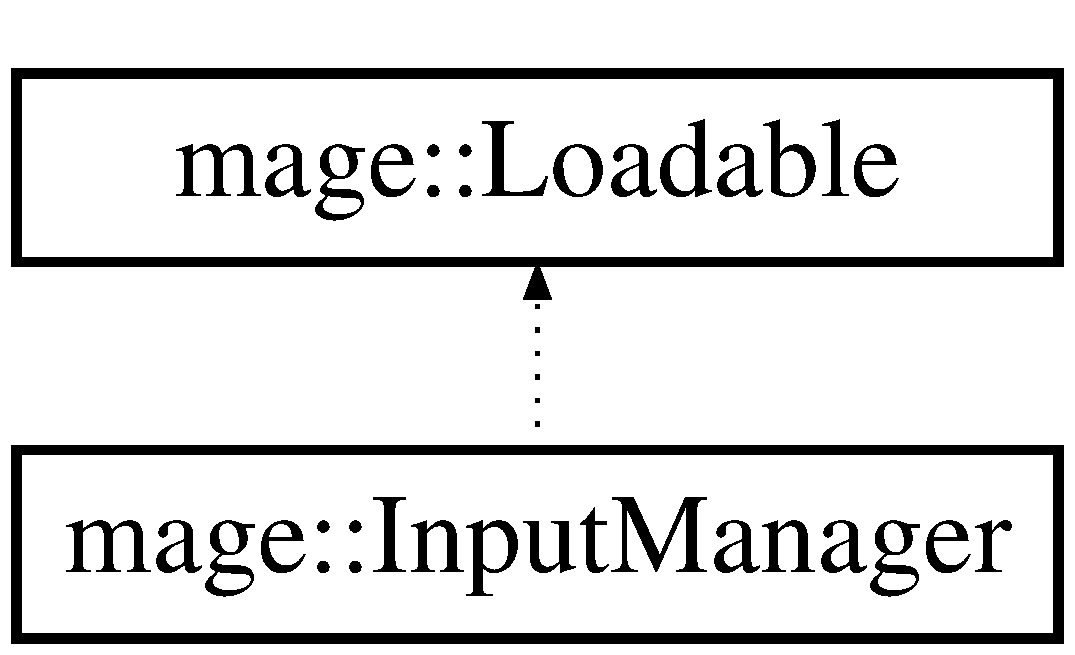
\includegraphics[height=2.000000cm]{classmage_1_1_input_manager}
\end{center}
\end{figure}
\subsection*{Public Member Functions}
\begin{DoxyCompactItemize}
\item 
const \hyperlink{classmage_1_1_keyboard}{Keyboard} $\ast$ \hyperlink{classmage_1_1_input_manager_a5b72139e30d1f3da6cda50f2989c1350}{Get\+Keyboard} () const
\item 
const \hyperlink{classmage_1_1_mouse}{Mouse} $\ast$ \hyperlink{classmage_1_1_input_manager_ad268916e07f44e40bf267efa0e673186}{Get\+Mouse} () const
\end{DoxyCompactItemize}
\subsection*{Protected Member Functions}
\begin{DoxyCompactItemize}
\item 
\hyperlink{classmage_1_1_input_manager_afc28df27a0251c242113a9761c007534}{Input\+Manager} (H\+W\+ND hwindow)
\item 
virtual \hyperlink{classmage_1_1_input_manager_a287ca0e91ec079227c102f7eadd5bb46}{$\sim$\+Input\+Manager} ()
\item 
H\+R\+E\+S\+U\+LT \hyperlink{classmage_1_1_input_manager_af3ca0717e37916463cc4f40c7d174b33}{Initialize\+DI} ()
\item 
H\+R\+E\+S\+U\+LT \hyperlink{classmage_1_1_input_manager_af16e113638fed35d34256f99bf061ef4}{Uninitialize\+DI} ()
\item 
H\+R\+E\+S\+U\+LT \hyperlink{classmage_1_1_input_manager_a34f114c4c667a4a14ce8236b35d308d8}{Initialize\+Input\+Systems} ()
\item 
H\+R\+E\+S\+U\+LT \hyperlink{classmage_1_1_input_manager_abecb06833973cab1ccabc7b28580209d}{Uninitialize\+Input\+Systems} ()
\item 
void \hyperlink{classmage_1_1_input_manager_a5e516969ff4ae9876b98c28f48f93726}{Update} ()
\end{DoxyCompactItemize}
\subsection*{Protected Attributes}
\begin{DoxyCompactItemize}
\item 
H\+W\+ND \hyperlink{classmage_1_1_input_manager_a07a1d3a593bc497c747c6d2e4605a229}{m\+\_\+hwindow}
\item 
I\+Direct\+Input8 $\ast$ \hyperlink{classmage_1_1_input_manager_a7341c72992efb7bee780111118f9589b}{m\+\_\+di}
\item 
\hyperlink{classmage_1_1_keyboard}{Keyboard} $\ast$ \hyperlink{classmage_1_1_input_manager_a04251723b39860d1436295ca74d5e997}{m\+\_\+keyboard}
\item 
\hyperlink{classmage_1_1_mouse}{Mouse} $\ast$ \hyperlink{classmage_1_1_input_manager_a41f41c1c021cc6dae422cb9abe7b8f87}{m\+\_\+mouse}
\end{DoxyCompactItemize}
\subsection*{Friends}
\begin{DoxyCompactItemize}
\item 
class \hyperlink{classmage_1_1_input_manager_a3e1914489e4bed4f9f23cdeab34a43dc}{Engine}
\end{DoxyCompactItemize}


\subsection{Detailed Description}
A class of input managers. 

\subsection{Constructor \& Destructor Documentation}
\hypertarget{classmage_1_1_input_manager_afc28df27a0251c242113a9761c007534}{}\label{classmage_1_1_input_manager_afc28df27a0251c242113a9761c007534} 
\index{mage\+::\+Input\+Manager@{mage\+::\+Input\+Manager}!Input\+Manager@{Input\+Manager}}
\index{Input\+Manager@{Input\+Manager}!mage\+::\+Input\+Manager@{mage\+::\+Input\+Manager}}
\subsubsection{\texorpdfstring{Input\+Manager()}{InputManager()}}
{\footnotesize\ttfamily mage\+::\+Input\+Manager\+::\+Input\+Manager (\begin{DoxyParamCaption}\item[{H\+W\+ND}]{hwindow }\end{DoxyParamCaption})\hspace{0.3cm}{\ttfamily [protected]}}

Constructs an input manager for the given window handle.


\begin{DoxyParams}[1]{Parameters}
\mbox{\tt in}  & {\em hwindow} & The handle of the parent window. \\
\hline
\end{DoxyParams}
\hypertarget{classmage_1_1_input_manager_a287ca0e91ec079227c102f7eadd5bb46}{}\label{classmage_1_1_input_manager_a287ca0e91ec079227c102f7eadd5bb46} 
\index{mage\+::\+Input\+Manager@{mage\+::\+Input\+Manager}!````~Input\+Manager@{$\sim$\+Input\+Manager}}
\index{````~Input\+Manager@{$\sim$\+Input\+Manager}!mage\+::\+Input\+Manager@{mage\+::\+Input\+Manager}}
\subsubsection{\texorpdfstring{$\sim$\+Input\+Manager()}{~InputManager()}}
{\footnotesize\ttfamily mage\+::\+Input\+Manager\+::$\sim$\+Input\+Manager (\begin{DoxyParamCaption}{ }\end{DoxyParamCaption})\hspace{0.3cm}{\ttfamily [protected]}, {\ttfamily [virtual]}}

Destructs this input manager. 

\subsection{Member Function Documentation}
\hypertarget{classmage_1_1_input_manager_a5b72139e30d1f3da6cda50f2989c1350}{}\label{classmage_1_1_input_manager_a5b72139e30d1f3da6cda50f2989c1350} 
\index{mage\+::\+Input\+Manager@{mage\+::\+Input\+Manager}!Get\+Keyboard@{Get\+Keyboard}}
\index{Get\+Keyboard@{Get\+Keyboard}!mage\+::\+Input\+Manager@{mage\+::\+Input\+Manager}}
\subsubsection{\texorpdfstring{Get\+Keyboard()}{GetKeyboard()}}
{\footnotesize\ttfamily const \hyperlink{classmage_1_1_keyboard}{Keyboard}$\ast$ mage\+::\+Input\+Manager\+::\+Get\+Keyboard (\begin{DoxyParamCaption}{ }\end{DoxyParamCaption}) const}

Returns the keyboard of this input manager.

\begin{DoxyReturn}{Returns}
A pointer to the keyboard of this input manager. 
\end{DoxyReturn}
\hypertarget{classmage_1_1_input_manager_ad268916e07f44e40bf267efa0e673186}{}\label{classmage_1_1_input_manager_ad268916e07f44e40bf267efa0e673186} 
\index{mage\+::\+Input\+Manager@{mage\+::\+Input\+Manager}!Get\+Mouse@{Get\+Mouse}}
\index{Get\+Mouse@{Get\+Mouse}!mage\+::\+Input\+Manager@{mage\+::\+Input\+Manager}}
\subsubsection{\texorpdfstring{Get\+Mouse()}{GetMouse()}}
{\footnotesize\ttfamily const \hyperlink{classmage_1_1_mouse}{Mouse}$\ast$ mage\+::\+Input\+Manager\+::\+Get\+Mouse (\begin{DoxyParamCaption}{ }\end{DoxyParamCaption}) const}

Returns the mouse of this input manager.

\begin{DoxyReturn}{Returns}
A pointer to the mouse of this input manager. 
\end{DoxyReturn}
\hypertarget{classmage_1_1_input_manager_af3ca0717e37916463cc4f40c7d174b33}{}\label{classmage_1_1_input_manager_af3ca0717e37916463cc4f40c7d174b33} 
\index{mage\+::\+Input\+Manager@{mage\+::\+Input\+Manager}!Initialize\+DI@{Initialize\+DI}}
\index{Initialize\+DI@{Initialize\+DI}!mage\+::\+Input\+Manager@{mage\+::\+Input\+Manager}}
\subsubsection{\texorpdfstring{Initialize\+D\+I()}{InitializeDI()}}
{\footnotesize\ttfamily H\+R\+E\+S\+U\+LT mage\+::\+Input\+Manager\+::\+Initialize\+DI (\begin{DoxyParamCaption}{ }\end{DoxyParamCaption})\hspace{0.3cm}{\ttfamily [protected]}}

Initializes the Direct\+Input object of this input manager.

\begin{DoxyReturn}{Returns}
A success/error value. 
\end{DoxyReturn}
\hypertarget{classmage_1_1_input_manager_a34f114c4c667a4a14ce8236b35d308d8}{}\label{classmage_1_1_input_manager_a34f114c4c667a4a14ce8236b35d308d8} 
\index{mage\+::\+Input\+Manager@{mage\+::\+Input\+Manager}!Initialize\+Input\+Systems@{Initialize\+Input\+Systems}}
\index{Initialize\+Input\+Systems@{Initialize\+Input\+Systems}!mage\+::\+Input\+Manager@{mage\+::\+Input\+Manager}}
\subsubsection{\texorpdfstring{Initialize\+Input\+Systems()}{InitializeInputSystems()}}
{\footnotesize\ttfamily H\+R\+E\+S\+U\+LT mage\+::\+Input\+Manager\+::\+Initialize\+Input\+Systems (\begin{DoxyParamCaption}{ }\end{DoxyParamCaption})\hspace{0.3cm}{\ttfamily [protected]}}

Initializes the different input systems of this input manager. \hypertarget{classmage_1_1_input_manager_af16e113638fed35d34256f99bf061ef4}{}\label{classmage_1_1_input_manager_af16e113638fed35d34256f99bf061ef4} 
\index{mage\+::\+Input\+Manager@{mage\+::\+Input\+Manager}!Uninitialize\+DI@{Uninitialize\+DI}}
\index{Uninitialize\+DI@{Uninitialize\+DI}!mage\+::\+Input\+Manager@{mage\+::\+Input\+Manager}}
\subsubsection{\texorpdfstring{Uninitialize\+D\+I()}{UninitializeDI()}}
{\footnotesize\ttfamily H\+R\+E\+S\+U\+LT mage\+::\+Input\+Manager\+::\+Uninitialize\+DI (\begin{DoxyParamCaption}{ }\end{DoxyParamCaption})\hspace{0.3cm}{\ttfamily [protected]}}

Uninitializes the Direct\+Input object of this input manager.

\begin{DoxyReturn}{Returns}
A success/error value. 
\end{DoxyReturn}
\hypertarget{classmage_1_1_input_manager_abecb06833973cab1ccabc7b28580209d}{}\label{classmage_1_1_input_manager_abecb06833973cab1ccabc7b28580209d} 
\index{mage\+::\+Input\+Manager@{mage\+::\+Input\+Manager}!Uninitialize\+Input\+Systems@{Uninitialize\+Input\+Systems}}
\index{Uninitialize\+Input\+Systems@{Uninitialize\+Input\+Systems}!mage\+::\+Input\+Manager@{mage\+::\+Input\+Manager}}
\subsubsection{\texorpdfstring{Uninitialize\+Input\+Systems()}{UninitializeInputSystems()}}
{\footnotesize\ttfamily H\+R\+E\+S\+U\+LT mage\+::\+Input\+Manager\+::\+Uninitialize\+Input\+Systems (\begin{DoxyParamCaption}{ }\end{DoxyParamCaption})\hspace{0.3cm}{\ttfamily [protected]}}

Initializes the different input systems of this manager. \hypertarget{classmage_1_1_input_manager_a5e516969ff4ae9876b98c28f48f93726}{}\label{classmage_1_1_input_manager_a5e516969ff4ae9876b98c28f48f93726} 
\index{mage\+::\+Input\+Manager@{mage\+::\+Input\+Manager}!Update@{Update}}
\index{Update@{Update}!mage\+::\+Input\+Manager@{mage\+::\+Input\+Manager}}
\subsubsection{\texorpdfstring{Update()}{Update()}}
{\footnotesize\ttfamily void mage\+::\+Input\+Manager\+::\+Update (\begin{DoxyParamCaption}{ }\end{DoxyParamCaption})\hspace{0.3cm}{\ttfamily [protected]}}

Updates the state of the input systems of this input manager. 

\subsection{Friends And Related Function Documentation}
\hypertarget{classmage_1_1_input_manager_a3e1914489e4bed4f9f23cdeab34a43dc}{}\label{classmage_1_1_input_manager_a3e1914489e4bed4f9f23cdeab34a43dc} 
\index{mage\+::\+Input\+Manager@{mage\+::\+Input\+Manager}!Engine@{Engine}}
\index{Engine@{Engine}!mage\+::\+Input\+Manager@{mage\+::\+Input\+Manager}}
\subsubsection{\texorpdfstring{Engine}{Engine}}
{\footnotesize\ttfamily friend class \hyperlink{classmage_1_1_engine}{Engine}\hspace{0.3cm}{\ttfamily [friend]}}



\subsection{Member Data Documentation}
\hypertarget{classmage_1_1_input_manager_a7341c72992efb7bee780111118f9589b}{}\label{classmage_1_1_input_manager_a7341c72992efb7bee780111118f9589b} 
\index{mage\+::\+Input\+Manager@{mage\+::\+Input\+Manager}!m\+\_\+di@{m\+\_\+di}}
\index{m\+\_\+di@{m\+\_\+di}!mage\+::\+Input\+Manager@{mage\+::\+Input\+Manager}}
\subsubsection{\texorpdfstring{m\+\_\+di}{m\_di}}
{\footnotesize\ttfamily I\+Direct\+Input8$\ast$ mage\+::\+Input\+Manager\+::m\+\_\+di\hspace{0.3cm}{\ttfamily [protected]}}

The Direct\+Input object of this input manager.

The methods of the I\+Direct\+Input8 interface are used to enumerate, create, and retrieve the status of Microsoft Direct\+Input device. \hypertarget{classmage_1_1_input_manager_a07a1d3a593bc497c747c6d2e4605a229}{}\label{classmage_1_1_input_manager_a07a1d3a593bc497c747c6d2e4605a229} 
\index{mage\+::\+Input\+Manager@{mage\+::\+Input\+Manager}!m\+\_\+hwindow@{m\+\_\+hwindow}}
\index{m\+\_\+hwindow@{m\+\_\+hwindow}!mage\+::\+Input\+Manager@{mage\+::\+Input\+Manager}}
\subsubsection{\texorpdfstring{m\+\_\+hwindow}{m\_hwindow}}
{\footnotesize\ttfamily H\+W\+ND mage\+::\+Input\+Manager\+::m\+\_\+hwindow\hspace{0.3cm}{\ttfamily [protected]}}

The handle of the parent window. \hypertarget{classmage_1_1_input_manager_a04251723b39860d1436295ca74d5e997}{}\label{classmage_1_1_input_manager_a04251723b39860d1436295ca74d5e997} 
\index{mage\+::\+Input\+Manager@{mage\+::\+Input\+Manager}!m\+\_\+keyboard@{m\+\_\+keyboard}}
\index{m\+\_\+keyboard@{m\+\_\+keyboard}!mage\+::\+Input\+Manager@{mage\+::\+Input\+Manager}}
\subsubsection{\texorpdfstring{m\+\_\+keyboard}{m\_keyboard}}
{\footnotesize\ttfamily \hyperlink{classmage_1_1_keyboard}{Keyboard}$\ast$ mage\+::\+Input\+Manager\+::m\+\_\+keyboard\hspace{0.3cm}{\ttfamily [protected]}}

A pointer to the keyboard of this input manager. \hypertarget{classmage_1_1_input_manager_a41f41c1c021cc6dae422cb9abe7b8f87}{}\label{classmage_1_1_input_manager_a41f41c1c021cc6dae422cb9abe7b8f87} 
\index{mage\+::\+Input\+Manager@{mage\+::\+Input\+Manager}!m\+\_\+mouse@{m\+\_\+mouse}}
\index{m\+\_\+mouse@{m\+\_\+mouse}!mage\+::\+Input\+Manager@{mage\+::\+Input\+Manager}}
\subsubsection{\texorpdfstring{m\+\_\+mouse}{m\_mouse}}
{\footnotesize\ttfamily \hyperlink{classmage_1_1_mouse}{Mouse}$\ast$ mage\+::\+Input\+Manager\+::m\+\_\+mouse\hspace{0.3cm}{\ttfamily [protected]}}

A pointer to the mouse of this input manager. 
\hypertarget{classmage_1_1_keyboard}{}\section{mage\+:\+:Keyboard Class Reference}
\label{classmage_1_1_keyboard}\index{mage\+::\+Keyboard@{mage\+::\+Keyboard}}


{\ttfamily \#include $<$keyboard.\+hpp$>$}

Inheritance diagram for mage\+:\+:Keyboard\+:\begin{figure}[H]
\begin{center}
\leavevmode
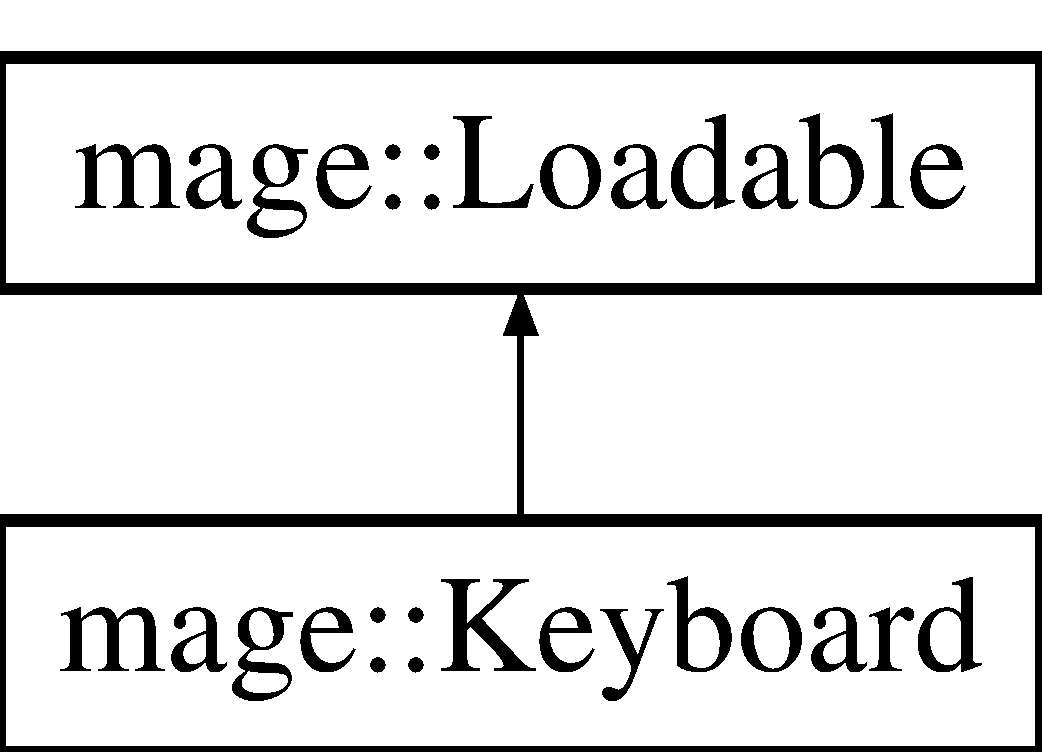
\includegraphics[height=2.000000cm]{classmage_1_1_keyboard}
\end{center}
\end{figure}
\subsection*{Public Member Functions}
\begin{DoxyCompactItemize}
\item 
\hyperlink{classmage_1_1_keyboard_af4afb6c7992b88f94f4b310c35f7e867}{Keyboard} (H\+W\+ND hwindow, \hyperlink{namespacemage_ae74f374780900893caa5555d1031fd79}{Com\+Ptr}$<$ I\+Direct\+Input8 $>$ di)
\item 
virtual \hyperlink{classmage_1_1_keyboard_a474715e04ba1ea8ae94ea519824d2e4a}{$\sim$\+Keyboard} ()
\item 
void \hyperlink{classmage_1_1_keyboard_abb5fd91a304f8bbf8b15ab1a277dafaf}{Update} ()
\item 
H\+W\+ND \hyperlink{classmage_1_1_keyboard_ab9d2244f94faccb9c745b07a8bebc888}{Get\+Handle} () const
\item 
bool \hyperlink{classmage_1_1_keyboard_a7ba5a3c47b7116afb5b3362739c2a278}{Get\+Key\+Press} (char key, bool ignore\+\_\+press\+\_\+stamp=false) const
\end{DoxyCompactItemize}
\subsection*{Protected Member Functions}
\begin{DoxyCompactItemize}
\item 
H\+R\+E\+S\+U\+LT \hyperlink{classmage_1_1_keyboard_a1d3211c7377529e570bb5cde900f73db}{Initialize\+Keyboard} (\hyperlink{namespacemage_ae74f374780900893caa5555d1031fd79}{Com\+Ptr}$<$ I\+Direct\+Input8 $>$ di)
\end{DoxyCompactItemize}
\subsection*{Protected Attributes}
\begin{DoxyCompactItemize}
\item 
uint64\+\_\+t \hyperlink{classmage_1_1_keyboard_a2c638a93d1f61d9d3578a0df8b6a1c39}{m\+\_\+press\+\_\+stamp}
\item 
\hyperlink{namespacemage_ae74f374780900893caa5555d1031fd79}{Com\+Ptr}$<$ I\+Direct\+Input\+Device8 $>$ \hyperlink{classmage_1_1_keyboard_a992b8b8caf0d858163e5e9af04302324}{m\+\_\+keyboard}
\item 
char \hyperlink{classmage_1_1_keyboard_ad3361790f2c9cc5ca19161f0c8e24acd}{m\+\_\+key\+\_\+state} \mbox{[}256\mbox{]}
\item 
uint64\+\_\+t \hyperlink{classmage_1_1_keyboard_a8eb4ce7e4e2395bb27d2ac9236655335}{m\+\_\+key\+\_\+press\+\_\+stamp} \mbox{[}256\mbox{]}
\end{DoxyCompactItemize}
\subsection*{Private Member Functions}
\begin{DoxyCompactItemize}
\item 
\hyperlink{classmage_1_1_keyboard_a39d07f8a5e37648ca9eba30aa55146bf}{Keyboard} (const \hyperlink{classmage_1_1_keyboard}{Keyboard} \&keyboard)=delete
\item 
\hyperlink{classmage_1_1_keyboard}{Keyboard} \& \hyperlink{classmage_1_1_keyboard_ae3ba98190c8c14ea894c676888825f35}{operator=} (const \hyperlink{classmage_1_1_keyboard}{Keyboard} \&keyboard)=delete
\end{DoxyCompactItemize}
\subsection*{Private Attributes}
\begin{DoxyCompactItemize}
\item 
H\+W\+ND \hyperlink{classmage_1_1_keyboard_aa7196c689dad6f5aaf35e3929de02791}{m\+\_\+hwindow}
\end{DoxyCompactItemize}


\subsection{Detailed Description}
A class of keyboards. 

\subsection{Constructor \& Destructor Documentation}
\hypertarget{classmage_1_1_keyboard_af4afb6c7992b88f94f4b310c35f7e867}{}\label{classmage_1_1_keyboard_af4afb6c7992b88f94f4b310c35f7e867} 
\index{mage\+::\+Keyboard@{mage\+::\+Keyboard}!Keyboard@{Keyboard}}
\index{Keyboard@{Keyboard}!mage\+::\+Keyboard@{mage\+::\+Keyboard}}
\subsubsection{\texorpdfstring{Keyboard()}{Keyboard()}\hspace{0.1cm}{\footnotesize\ttfamily [1/2]}}
{\footnotesize\ttfamily mage\+::\+Keyboard\+::\+Keyboard (\begin{DoxyParamCaption}\item[{H\+W\+ND}]{hwindow,  }\item[{\hyperlink{namespacemage_ae74f374780900893caa5555d1031fd79}{Com\+Ptr}$<$ I\+Direct\+Input8 $>$}]{di }\end{DoxyParamCaption})}

Constructs a keyboard.


\begin{DoxyParams}[1]{Parameters}
\mbox{\tt in}  & {\em hwindow} & The handle of the parent window. \\
\hline
\mbox{\tt in}  & {\em di} & A pointer to a direct input object. \\
\hline
\end{DoxyParams}
\hypertarget{classmage_1_1_keyboard_a474715e04ba1ea8ae94ea519824d2e4a}{}\label{classmage_1_1_keyboard_a474715e04ba1ea8ae94ea519824d2e4a} 
\index{mage\+::\+Keyboard@{mage\+::\+Keyboard}!````~Keyboard@{$\sim$\+Keyboard}}
\index{````~Keyboard@{$\sim$\+Keyboard}!mage\+::\+Keyboard@{mage\+::\+Keyboard}}
\subsubsection{\texorpdfstring{$\sim$\+Keyboard()}{~Keyboard()}}
{\footnotesize\ttfamily virtual mage\+::\+Keyboard\+::$\sim$\+Keyboard (\begin{DoxyParamCaption}{ }\end{DoxyParamCaption})\hspace{0.3cm}{\ttfamily [virtual]}}

Destructs this keyboard. \hypertarget{classmage_1_1_keyboard_a39d07f8a5e37648ca9eba30aa55146bf}{}\label{classmage_1_1_keyboard_a39d07f8a5e37648ca9eba30aa55146bf} 
\index{mage\+::\+Keyboard@{mage\+::\+Keyboard}!Keyboard@{Keyboard}}
\index{Keyboard@{Keyboard}!mage\+::\+Keyboard@{mage\+::\+Keyboard}}
\subsubsection{\texorpdfstring{Keyboard()}{Keyboard()}\hspace{0.1cm}{\footnotesize\ttfamily [2/2]}}
{\footnotesize\ttfamily mage\+::\+Keyboard\+::\+Keyboard (\begin{DoxyParamCaption}\item[{const \hyperlink{classmage_1_1_keyboard}{Keyboard} \&}]{keyboard }\end{DoxyParamCaption})\hspace{0.3cm}{\ttfamily [private]}, {\ttfamily [delete]}}

Constructs a keyboard from the given keyboard.


\begin{DoxyParams}[1]{Parameters}
\mbox{\tt in}  & {\em keyboard} & A reference to the keyboard. \\
\hline
\end{DoxyParams}


\subsection{Member Function Documentation}
\hypertarget{classmage_1_1_keyboard_ab9d2244f94faccb9c745b07a8bebc888}{}\label{classmage_1_1_keyboard_ab9d2244f94faccb9c745b07a8bebc888} 
\index{mage\+::\+Keyboard@{mage\+::\+Keyboard}!Get\+Handle@{Get\+Handle}}
\index{Get\+Handle@{Get\+Handle}!mage\+::\+Keyboard@{mage\+::\+Keyboard}}
\subsubsection{\texorpdfstring{Get\+Handle()}{GetHandle()}}
{\footnotesize\ttfamily H\+W\+ND mage\+::\+Keyboard\+::\+Get\+Handle (\begin{DoxyParamCaption}{ }\end{DoxyParamCaption}) const}

Returns the window handle of this keyboard.

\begin{DoxyReturn}{Returns}
The window handle of this keyboard. 
\end{DoxyReturn}
\hypertarget{classmage_1_1_keyboard_a7ba5a3c47b7116afb5b3362739c2a278}{}\label{classmage_1_1_keyboard_a7ba5a3c47b7116afb5b3362739c2a278} 
\index{mage\+::\+Keyboard@{mage\+::\+Keyboard}!Get\+Key\+Press@{Get\+Key\+Press}}
\index{Get\+Key\+Press@{Get\+Key\+Press}!mage\+::\+Keyboard@{mage\+::\+Keyboard}}
\subsubsection{\texorpdfstring{Get\+Key\+Press()}{GetKeyPress()}}
{\footnotesize\ttfamily bool mage\+::\+Keyboard\+::\+Get\+Key\+Press (\begin{DoxyParamCaption}\item[{char}]{key,  }\item[{bool}]{ignore\+\_\+press\+\_\+stamp = {\ttfamily false} }\end{DoxyParamCaption}) const}

Checks whether the given key of this keyboard is pressed.


\begin{DoxyParams}[1]{Parameters}
\mbox{\tt in}  & {\em key} & The key. \\
\hline
\mbox{\tt in}  & {\em ignore\+\_\+press\+\_\+stamp} & Flag indicating whether press stamps should be ignored. Consistent presses will return false when using the press stamp. \\
\hline
\end{DoxyParams}
\begin{DoxyReturn}{Returns}
{\ttfamily true} if the given key of this keyboard is pressed. {\ttfamily false} otherwise. 
\end{DoxyReturn}
\hypertarget{classmage_1_1_keyboard_a1d3211c7377529e570bb5cde900f73db}{}\label{classmage_1_1_keyboard_a1d3211c7377529e570bb5cde900f73db} 
\index{mage\+::\+Keyboard@{mage\+::\+Keyboard}!Initialize\+Keyboard@{Initialize\+Keyboard}}
\index{Initialize\+Keyboard@{Initialize\+Keyboard}!mage\+::\+Keyboard@{mage\+::\+Keyboard}}
\subsubsection{\texorpdfstring{Initialize\+Keyboard()}{InitializeKeyboard()}}
{\footnotesize\ttfamily H\+R\+E\+S\+U\+LT mage\+::\+Keyboard\+::\+Initialize\+Keyboard (\begin{DoxyParamCaption}\item[{\hyperlink{namespacemage_ae74f374780900893caa5555d1031fd79}{Com\+Ptr}$<$ I\+Direct\+Input8 $>$}]{di }\end{DoxyParamCaption})\hspace{0.3cm}{\ttfamily [protected]}}

Initializes the keyboard device of this keyboard.


\begin{DoxyParams}[1]{Parameters}
\mbox{\tt in}  & {\em di} & A pointer to a direct input object. \\
\hline
\end{DoxyParams}
\begin{DoxyReturn}{Returns}
A success/error value. 
\end{DoxyReturn}
\hypertarget{classmage_1_1_keyboard_ae3ba98190c8c14ea894c676888825f35}{}\label{classmage_1_1_keyboard_ae3ba98190c8c14ea894c676888825f35} 
\index{mage\+::\+Keyboard@{mage\+::\+Keyboard}!operator=@{operator=}}
\index{operator=@{operator=}!mage\+::\+Keyboard@{mage\+::\+Keyboard}}
\subsubsection{\texorpdfstring{operator=()}{operator=()}}
{\footnotesize\ttfamily \hyperlink{classmage_1_1_keyboard}{Keyboard}\& mage\+::\+Keyboard\+::operator= (\begin{DoxyParamCaption}\item[{const \hyperlink{classmage_1_1_keyboard}{Keyboard} \&}]{keyboard }\end{DoxyParamCaption})\hspace{0.3cm}{\ttfamily [private]}, {\ttfamily [delete]}}

Copies the given keyboard to this keyboard.


\begin{DoxyParams}[1]{Parameters}
\mbox{\tt in}  & {\em keyboard} & A reference to the keyboard to copy from. \\
\hline
\end{DoxyParams}
\begin{DoxyReturn}{Returns}
A reference to the copy of the given keyboard (i.\+e. this keyboard). 
\end{DoxyReturn}
\hypertarget{classmage_1_1_keyboard_abb5fd91a304f8bbf8b15ab1a277dafaf}{}\label{classmage_1_1_keyboard_abb5fd91a304f8bbf8b15ab1a277dafaf} 
\index{mage\+::\+Keyboard@{mage\+::\+Keyboard}!Update@{Update}}
\index{Update@{Update}!mage\+::\+Keyboard@{mage\+::\+Keyboard}}
\subsubsection{\texorpdfstring{Update()}{Update()}}
{\footnotesize\ttfamily void mage\+::\+Keyboard\+::\+Update (\begin{DoxyParamCaption}{ }\end{DoxyParamCaption})}

Updates the state of this keyboard. 

\subsection{Member Data Documentation}
\hypertarget{classmage_1_1_keyboard_aa7196c689dad6f5aaf35e3929de02791}{}\label{classmage_1_1_keyboard_aa7196c689dad6f5aaf35e3929de02791} 
\index{mage\+::\+Keyboard@{mage\+::\+Keyboard}!m\+\_\+hwindow@{m\+\_\+hwindow}}
\index{m\+\_\+hwindow@{m\+\_\+hwindow}!mage\+::\+Keyboard@{mage\+::\+Keyboard}}
\subsubsection{\texorpdfstring{m\+\_\+hwindow}{m\_hwindow}}
{\footnotesize\ttfamily H\+W\+ND mage\+::\+Keyboard\+::m\+\_\+hwindow\hspace{0.3cm}{\ttfamily [private]}}

The handle of the parent window. \hypertarget{classmage_1_1_keyboard_a8eb4ce7e4e2395bb27d2ac9236655335}{}\label{classmage_1_1_keyboard_a8eb4ce7e4e2395bb27d2ac9236655335} 
\index{mage\+::\+Keyboard@{mage\+::\+Keyboard}!m\+\_\+key\+\_\+press\+\_\+stamp@{m\+\_\+key\+\_\+press\+\_\+stamp}}
\index{m\+\_\+key\+\_\+press\+\_\+stamp@{m\+\_\+key\+\_\+press\+\_\+stamp}!mage\+::\+Keyboard@{mage\+::\+Keyboard}}
\subsubsection{\texorpdfstring{m\+\_\+key\+\_\+press\+\_\+stamp}{m\_key\_press\_stamp}}
{\footnotesize\ttfamily uint64\+\_\+t mage\+::\+Keyboard\+::m\+\_\+key\+\_\+press\+\_\+stamp\mbox{[}256\mbox{]}\hspace{0.3cm}{\ttfamily [mutable]}, {\ttfamily [protected]}}

Stamps the keys pressed in the last frame of this keyboard. \hypertarget{classmage_1_1_keyboard_ad3361790f2c9cc5ca19161f0c8e24acd}{}\label{classmage_1_1_keyboard_ad3361790f2c9cc5ca19161f0c8e24acd} 
\index{mage\+::\+Keyboard@{mage\+::\+Keyboard}!m\+\_\+key\+\_\+state@{m\+\_\+key\+\_\+state}}
\index{m\+\_\+key\+\_\+state@{m\+\_\+key\+\_\+state}!mage\+::\+Keyboard@{mage\+::\+Keyboard}}
\subsubsection{\texorpdfstring{m\+\_\+key\+\_\+state}{m\_key\_state}}
{\footnotesize\ttfamily char mage\+::\+Keyboard\+::m\+\_\+key\+\_\+state\mbox{[}256\mbox{]}\hspace{0.3cm}{\ttfamily [protected]}}

\hyperlink{classmage_1_1_state}{State} of the keys of this keyboard. \hypertarget{classmage_1_1_keyboard_a992b8b8caf0d858163e5e9af04302324}{}\label{classmage_1_1_keyboard_a992b8b8caf0d858163e5e9af04302324} 
\index{mage\+::\+Keyboard@{mage\+::\+Keyboard}!m\+\_\+keyboard@{m\+\_\+keyboard}}
\index{m\+\_\+keyboard@{m\+\_\+keyboard}!mage\+::\+Keyboard@{mage\+::\+Keyboard}}
\subsubsection{\texorpdfstring{m\+\_\+keyboard}{m\_keyboard}}
{\footnotesize\ttfamily \hyperlink{namespacemage_ae74f374780900893caa5555d1031fd79}{Com\+Ptr}$<$ I\+Direct\+Input\+Device8 $>$ mage\+::\+Keyboard\+::m\+\_\+keyboard\hspace{0.3cm}{\ttfamily [protected]}}

The Direct\+Input keyboard device of this keyboard.

The methods of the I\+Direct\+Input\+Device8 interface are used to gain and release access to Microsoft Direct\+Input devices, manage device properties and information, set behavior, perform initialization, create and play force-\/feedback effects, and invoke a device\textquotesingle{}s control panel. \hypertarget{classmage_1_1_keyboard_a2c638a93d1f61d9d3578a0df8b6a1c39}{}\label{classmage_1_1_keyboard_a2c638a93d1f61d9d3578a0df8b6a1c39} 
\index{mage\+::\+Keyboard@{mage\+::\+Keyboard}!m\+\_\+press\+\_\+stamp@{m\+\_\+press\+\_\+stamp}}
\index{m\+\_\+press\+\_\+stamp@{m\+\_\+press\+\_\+stamp}!mage\+::\+Keyboard@{mage\+::\+Keyboard}}
\subsubsection{\texorpdfstring{m\+\_\+press\+\_\+stamp}{m\_press\_stamp}}
{\footnotesize\ttfamily uint64\+\_\+t mage\+::\+Keyboard\+::m\+\_\+press\+\_\+stamp\hspace{0.3cm}{\ttfamily [protected]}}

The current press stamp (incremented every frame). 
\hypertarget{classmage_1_1_loadable}{}\section{mage\+:\+:Loadable Class Reference}
\label{classmage_1_1_loadable}\index{mage\+::\+Loadable@{mage\+::\+Loadable}}


{\ttfamily \#include $<$loadable.\+hpp$>$}

Inheritance diagram for mage\+:\+:Loadable\+:\begin{figure}[H]
\begin{center}
\leavevmode
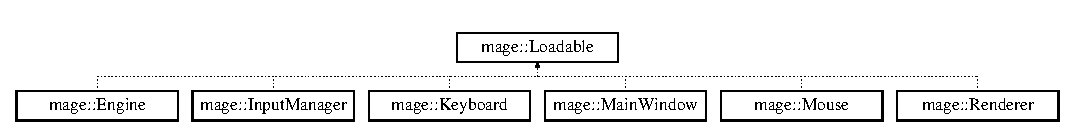
\includegraphics[height=1.393035cm]{classmage_1_1_loadable}
\end{center}
\end{figure}
\subsection*{Public Member Functions}
\begin{DoxyCompactItemize}
\item 
bool \hyperlink{classmage_1_1_loadable_a53cfa5beb9b44bbcda0d6166a54b8cb6}{Is\+Loaded} () const
\end{DoxyCompactItemize}
\subsection*{Protected Member Functions}
\begin{DoxyCompactItemize}
\item 
\hyperlink{classmage_1_1_loadable_afbdcb287b5e20583899a27a1c244bc7d}{Loadable} (bool loaded=false)
\item 
\hyperlink{classmage_1_1_loadable_a21364449c045d579cb6090347d83cd54}{Loadable} (const \hyperlink{classmage_1_1_loadable}{Loadable} \&loadable)=default
\item 
virtual \hyperlink{classmage_1_1_loadable_a7f51b5e1065ebe4dd1da7ef9c9966546}{$\sim$\+Loadable} ()=default
\item 
\hyperlink{classmage_1_1_loadable}{Loadable} \& \hyperlink{classmage_1_1_loadable_a82277616525b6ed9b1e19fd2dcdb4c0d}{operator=} (const \hyperlink{classmage_1_1_loadable}{Loadable} \&loadable)=default
\item 
void \hyperlink{classmage_1_1_loadable_a932ff8b287c8e68e30a13804cba08ff2}{Set\+Loaded} (bool loaded=true)
\end{DoxyCompactItemize}
\subsection*{Private Attributes}
\begin{DoxyCompactItemize}
\item 
bool \hyperlink{classmage_1_1_loadable_a993963fbfeb0f2e2ab9616bf7ef6a0f7}{m\+\_\+loaded}
\end{DoxyCompactItemize}


\subsection{Detailed Description}
A class of loadables. 

\subsection{Constructor \& Destructor Documentation}
\hypertarget{classmage_1_1_loadable_afbdcb287b5e20583899a27a1c244bc7d}{}\label{classmage_1_1_loadable_afbdcb287b5e20583899a27a1c244bc7d} 
\index{mage\+::\+Loadable@{mage\+::\+Loadable}!Loadable@{Loadable}}
\index{Loadable@{Loadable}!mage\+::\+Loadable@{mage\+::\+Loadable}}
\subsubsection{\texorpdfstring{Loadable()}{Loadable()}\hspace{0.1cm}{\footnotesize\ttfamily [1/2]}}
{\footnotesize\ttfamily mage\+::\+Loadable\+::\+Loadable (\begin{DoxyParamCaption}\item[{bool}]{loaded = {\ttfamily false} }\end{DoxyParamCaption})\hspace{0.3cm}{\ttfamily [protected]}}

Constructs a loadable.


\begin{DoxyParams}[1]{Parameters}
\mbox{\tt in}  & {\em loaded} & Flag indicating wether the loadable is loaded. \\
\hline
\end{DoxyParams}
\hypertarget{classmage_1_1_loadable_a21364449c045d579cb6090347d83cd54}{}\label{classmage_1_1_loadable_a21364449c045d579cb6090347d83cd54} 
\index{mage\+::\+Loadable@{mage\+::\+Loadable}!Loadable@{Loadable}}
\index{Loadable@{Loadable}!mage\+::\+Loadable@{mage\+::\+Loadable}}
\subsubsection{\texorpdfstring{Loadable()}{Loadable()}\hspace{0.1cm}{\footnotesize\ttfamily [2/2]}}
{\footnotesize\ttfamily mage\+::\+Loadable\+::\+Loadable (\begin{DoxyParamCaption}\item[{const \hyperlink{classmage_1_1_loadable}{Loadable} \&}]{loadable }\end{DoxyParamCaption})\hspace{0.3cm}{\ttfamily [protected]}, {\ttfamily [default]}}

Constructs a loadable from the given loadable.


\begin{DoxyParams}[1]{Parameters}
\mbox{\tt in}  & {\em loadable} & A reference to the loadable. \\
\hline
\end{DoxyParams}
\hypertarget{classmage_1_1_loadable_a7f51b5e1065ebe4dd1da7ef9c9966546}{}\label{classmage_1_1_loadable_a7f51b5e1065ebe4dd1da7ef9c9966546} 
\index{mage\+::\+Loadable@{mage\+::\+Loadable}!````~Loadable@{$\sim$\+Loadable}}
\index{````~Loadable@{$\sim$\+Loadable}!mage\+::\+Loadable@{mage\+::\+Loadable}}
\subsubsection{\texorpdfstring{$\sim$\+Loadable()}{~Loadable()}}
{\footnotesize\ttfamily virtual mage\+::\+Loadable\+::$\sim$\+Loadable (\begin{DoxyParamCaption}{ }\end{DoxyParamCaption})\hspace{0.3cm}{\ttfamily [protected]}, {\ttfamily [virtual]}, {\ttfamily [default]}}

Destructs this loadable. 

\subsection{Member Function Documentation}
\hypertarget{classmage_1_1_loadable_a53cfa5beb9b44bbcda0d6166a54b8cb6}{}\label{classmage_1_1_loadable_a53cfa5beb9b44bbcda0d6166a54b8cb6} 
\index{mage\+::\+Loadable@{mage\+::\+Loadable}!Is\+Loaded@{Is\+Loaded}}
\index{Is\+Loaded@{Is\+Loaded}!mage\+::\+Loadable@{mage\+::\+Loadable}}
\subsubsection{\texorpdfstring{Is\+Loaded()}{IsLoaded()}}
{\footnotesize\ttfamily bool mage\+::\+Loadable\+::\+Is\+Loaded (\begin{DoxyParamCaption}{ }\end{DoxyParamCaption}) const}

Checks wether this loadable is loaded.

\begin{DoxyReturn}{Returns}
{\ttfamily true} if this loadable is loaded. {\ttfamily false} otherwise. 
\end{DoxyReturn}
\hypertarget{classmage_1_1_loadable_a82277616525b6ed9b1e19fd2dcdb4c0d}{}\label{classmage_1_1_loadable_a82277616525b6ed9b1e19fd2dcdb4c0d} 
\index{mage\+::\+Loadable@{mage\+::\+Loadable}!operator=@{operator=}}
\index{operator=@{operator=}!mage\+::\+Loadable@{mage\+::\+Loadable}}
\subsubsection{\texorpdfstring{operator=()}{operator=()}}
{\footnotesize\ttfamily \hyperlink{classmage_1_1_loadable}{Loadable}\& mage\+::\+Loadable\+::operator= (\begin{DoxyParamCaption}\item[{const \hyperlink{classmage_1_1_loadable}{Loadable} \&}]{loadable }\end{DoxyParamCaption})\hspace{0.3cm}{\ttfamily [protected]}, {\ttfamily [default]}}

Copies the given loadable to this loadable.


\begin{DoxyParams}[1]{Parameters}
\mbox{\tt in}  & {\em loadable} & A reference to the loadable to copy from. \\
\hline
\end{DoxyParams}
\begin{DoxyReturn}{Returns}
A reference to the copy of the given loadable (i.\+e. this loadable). 
\end{DoxyReturn}
\hypertarget{classmage_1_1_loadable_a932ff8b287c8e68e30a13804cba08ff2}{}\label{classmage_1_1_loadable_a932ff8b287c8e68e30a13804cba08ff2} 
\index{mage\+::\+Loadable@{mage\+::\+Loadable}!Set\+Loaded@{Set\+Loaded}}
\index{Set\+Loaded@{Set\+Loaded}!mage\+::\+Loadable@{mage\+::\+Loadable}}
\subsubsection{\texorpdfstring{Set\+Loaded()}{SetLoaded()}}
{\footnotesize\ttfamily void mage\+::\+Loadable\+::\+Set\+Loaded (\begin{DoxyParamCaption}\item[{bool}]{loaded = {\ttfamily true} }\end{DoxyParamCaption})\hspace{0.3cm}{\ttfamily [protected]}}

Set the state of this loadable to the given value.


\begin{DoxyParams}[1]{Parameters}
\mbox{\tt in}  & {\em loaded} & Flag indicating wether this loadable is loaded. \\
\hline
\end{DoxyParams}


\subsection{Member Data Documentation}
\hypertarget{classmage_1_1_loadable_a993963fbfeb0f2e2ab9616bf7ef6a0f7}{}\label{classmage_1_1_loadable_a993963fbfeb0f2e2ab9616bf7ef6a0f7} 
\index{mage\+::\+Loadable@{mage\+::\+Loadable}!m\+\_\+loaded@{m\+\_\+loaded}}
\index{m\+\_\+loaded@{m\+\_\+loaded}!mage\+::\+Loadable@{mage\+::\+Loadable}}
\subsubsection{\texorpdfstring{m\+\_\+loaded}{m\_loaded}}
{\footnotesize\ttfamily bool mage\+::\+Loadable\+::m\+\_\+loaded\hspace{0.3cm}{\ttfamily [private]}}

Flag indicating wether this loadable is loaded. 
\hypertarget{structmage_1_1_logging_configuration}{}\section{mage\+:\+:Logging\+Configuration Struct Reference}
\label{structmage_1_1_logging_configuration}\index{mage\+::\+Logging\+Configuration@{mage\+::\+Logging\+Configuration}}


{\ttfamily \#include $<$logging.\+hpp$>$}

\subsection*{Public Member Functions}
\begin{DoxyCompactItemize}
\item 
\hyperlink{structmage_1_1_logging_configuration_a3d397c3ce26c1c42c9ae4a391391c6f9}{Logging\+Configuration} ()
\item 
bool \hyperlink{structmage_1_1_logging_configuration_ac081313b7a9440bcd73b6a9b69ff3452}{Is\+Quiet} () const
\item 
bool \hyperlink{structmage_1_1_logging_configuration_a13d91de33f888eee31f4d4e6b1237675}{Is\+Verbose} () const
\end{DoxyCompactItemize}
\subsection*{Private Attributes}
\begin{DoxyCompactItemize}
\item 
bool \hyperlink{structmage_1_1_logging_configuration_a38f457d5db84d15e008841ca8653b47c}{m\+\_\+quiet}
\item 
bool \hyperlink{structmage_1_1_logging_configuration_a60f052c2bb702d8153188e93f00427ac}{m\+\_\+verbose}
\end{DoxyCompactItemize}


\subsection{Detailed Description}
A struct of logging configurations of the engine processing. 

\subsection{Constructor \& Destructor Documentation}
\hypertarget{structmage_1_1_logging_configuration_a3d397c3ce26c1c42c9ae4a391391c6f9}{}\label{structmage_1_1_logging_configuration_a3d397c3ce26c1c42c9ae4a391391c6f9} 
\index{mage\+::\+Logging\+Configuration@{mage\+::\+Logging\+Configuration}!Logging\+Configuration@{Logging\+Configuration}}
\index{Logging\+Configuration@{Logging\+Configuration}!mage\+::\+Logging\+Configuration@{mage\+::\+Logging\+Configuration}}
\subsubsection{\texorpdfstring{Logging\+Configuration()}{LoggingConfiguration()}}
{\footnotesize\ttfamily mage\+::\+Logging\+Configuration\+::\+Logging\+Configuration (\begin{DoxyParamCaption}{ }\end{DoxyParamCaption})}

Constructs a new logging configuration. 

\subsection{Member Function Documentation}
\hypertarget{structmage_1_1_logging_configuration_ac081313b7a9440bcd73b6a9b69ff3452}{}\label{structmage_1_1_logging_configuration_ac081313b7a9440bcd73b6a9b69ff3452} 
\index{mage\+::\+Logging\+Configuration@{mage\+::\+Logging\+Configuration}!Is\+Quiet@{Is\+Quiet}}
\index{Is\+Quiet@{Is\+Quiet}!mage\+::\+Logging\+Configuration@{mage\+::\+Logging\+Configuration}}
\subsubsection{\texorpdfstring{Is\+Quiet()}{IsQuiet()}}
{\footnotesize\ttfamily bool mage\+::\+Logging\+Configuration\+::\+Is\+Quiet (\begin{DoxyParamCaption}{ }\end{DoxyParamCaption}) const}

Checks whether the logging of the engine processing is quiet.

\begin{DoxyReturn}{Returns}
{\ttfamily true} if the logging of the engine processing is quiet. {\ttfamily false} otherwise. 
\end{DoxyReturn}
\hypertarget{structmage_1_1_logging_configuration_a13d91de33f888eee31f4d4e6b1237675}{}\label{structmage_1_1_logging_configuration_a13d91de33f888eee31f4d4e6b1237675} 
\index{mage\+::\+Logging\+Configuration@{mage\+::\+Logging\+Configuration}!Is\+Verbose@{Is\+Verbose}}
\index{Is\+Verbose@{Is\+Verbose}!mage\+::\+Logging\+Configuration@{mage\+::\+Logging\+Configuration}}
\subsubsection{\texorpdfstring{Is\+Verbose()}{IsVerbose()}}
{\footnotesize\ttfamily bool mage\+::\+Logging\+Configuration\+::\+Is\+Verbose (\begin{DoxyParamCaption}{ }\end{DoxyParamCaption}) const}

Checks wheter the logging of the engine processing is verbose.

\begin{DoxyReturn}{Returns}
{\ttfamily true} if the logging of the engine processing is verbose. {\ttfamily false} otherwise. 
\end{DoxyReturn}


\subsection{Member Data Documentation}
\hypertarget{structmage_1_1_logging_configuration_a38f457d5db84d15e008841ca8653b47c}{}\label{structmage_1_1_logging_configuration_a38f457d5db84d15e008841ca8653b47c} 
\index{mage\+::\+Logging\+Configuration@{mage\+::\+Logging\+Configuration}!m\+\_\+quiet@{m\+\_\+quiet}}
\index{m\+\_\+quiet@{m\+\_\+quiet}!mage\+::\+Logging\+Configuration@{mage\+::\+Logging\+Configuration}}
\subsubsection{\texorpdfstring{m\+\_\+quiet}{m\_quiet}}
{\footnotesize\ttfamily bool mage\+::\+Logging\+Configuration\+::m\+\_\+quiet\hspace{0.3cm}{\ttfamily [private]}}

Flag indicating the logging of the engine processing is quiet. \hypertarget{structmage_1_1_logging_configuration_a60f052c2bb702d8153188e93f00427ac}{}\label{structmage_1_1_logging_configuration_a60f052c2bb702d8153188e93f00427ac} 
\index{mage\+::\+Logging\+Configuration@{mage\+::\+Logging\+Configuration}!m\+\_\+verbose@{m\+\_\+verbose}}
\index{m\+\_\+verbose@{m\+\_\+verbose}!mage\+::\+Logging\+Configuration@{mage\+::\+Logging\+Configuration}}
\subsubsection{\texorpdfstring{m\+\_\+verbose}{m\_verbose}}
{\footnotesize\ttfamily bool mage\+::\+Logging\+Configuration\+::m\+\_\+verbose\hspace{0.3cm}{\ttfamily [private]}}

Flag indicating the logging of the engine processing is verbose. 
\hypertarget{structmage_1_1_l_vertex}{}\section{mage\+:\+:L\+Vertex Struct Reference}
\label{structmage_1_1_l_vertex}\index{mage\+::\+L\+Vertex@{mage\+::\+L\+Vertex}}


{\ttfamily \#include $<$geometry.\+hpp$>$}

\subsection*{Public Member Functions}
\begin{DoxyCompactItemize}
\item 
\hyperlink{structmage_1_1_l_vertex_abfc69fb38d5f37b07d1c420a23a3e7f9}{L\+Vertex} ()
\item 
\hyperlink{structmage_1_1_l_vertex_a262af68c7c50c1003bcbd941b504fe70}{L\+Vertex} (X\+M\+F\+L\+O\+A\+T3 \hyperlink{structmage_1_1_l_vertex_afdf01d172b1992d4e4f37b9ad9fb2d27}{p}, X\+M\+F\+L\+O\+A\+T4 \hyperlink{structmage_1_1_l_vertex_abfe65c089e650ad20ed41de8e2b585dd}{diffuse}, float \hyperlink{structmage_1_1_l_vertex_a820b1dba91a65e4be9a41c4297970dd6}{tu}, float \hyperlink{structmage_1_1_l_vertex_ab5e712d5befd3b8e3b58c772e6d3bf50}{tv})
\end{DoxyCompactItemize}
\subsection*{Public Attributes}
\begin{DoxyCompactItemize}
\item 
X\+M\+F\+L\+O\+A\+T3 \hyperlink{structmage_1_1_l_vertex_afdf01d172b1992d4e4f37b9ad9fb2d27}{p}
\item 
X\+M\+F\+L\+O\+A\+T4 \hyperlink{structmage_1_1_l_vertex_abfe65c089e650ad20ed41de8e2b585dd}{diffuse}
\item 
float \hyperlink{structmage_1_1_l_vertex_a820b1dba91a65e4be9a41c4297970dd6}{tu}
\item 
float \hyperlink{structmage_1_1_l_vertex_ab5e712d5befd3b8e3b58c772e6d3bf50}{tv}
\end{DoxyCompactItemize}


\subsection{Detailed Description}
A struct of lit vertices. 

\subsection{Constructor \& Destructor Documentation}
\hypertarget{structmage_1_1_l_vertex_abfc69fb38d5f37b07d1c420a23a3e7f9}{}\label{structmage_1_1_l_vertex_abfc69fb38d5f37b07d1c420a23a3e7f9} 
\index{mage\+::\+L\+Vertex@{mage\+::\+L\+Vertex}!L\+Vertex@{L\+Vertex}}
\index{L\+Vertex@{L\+Vertex}!mage\+::\+L\+Vertex@{mage\+::\+L\+Vertex}}
\subsubsection{\texorpdfstring{L\+Vertex()}{LVertex()}\hspace{0.1cm}{\footnotesize\ttfamily [1/2]}}
{\footnotesize\ttfamily mage\+::\+L\+Vertex\+::\+L\+Vertex (\begin{DoxyParamCaption}{ }\end{DoxyParamCaption})}

Constructs a lit vertex. \hypertarget{structmage_1_1_l_vertex_a262af68c7c50c1003bcbd941b504fe70}{}\label{structmage_1_1_l_vertex_a262af68c7c50c1003bcbd941b504fe70} 
\index{mage\+::\+L\+Vertex@{mage\+::\+L\+Vertex}!L\+Vertex@{L\+Vertex}}
\index{L\+Vertex@{L\+Vertex}!mage\+::\+L\+Vertex@{mage\+::\+L\+Vertex}}
\subsubsection{\texorpdfstring{L\+Vertex()}{LVertex()}\hspace{0.1cm}{\footnotesize\ttfamily [2/2]}}
{\footnotesize\ttfamily mage\+::\+L\+Vertex\+::\+L\+Vertex (\begin{DoxyParamCaption}\item[{X\+M\+F\+L\+O\+A\+T3}]{p,  }\item[{X\+M\+F\+L\+O\+A\+T4}]{diffuse,  }\item[{float}]{tu,  }\item[{float}]{tv }\end{DoxyParamCaption})}

Constructs a lit vertex.


\begin{DoxyParams}[1]{Parameters}
\mbox{\tt in}  & {\em p} & Position of the lit vertex (in world space). \\
\hline
\mbox{\tt in}  & {\em diffuse} & Diffuse colour of the lit vertex. \\
\hline
\mbox{\tt in}  & {\em tu} & Texture u coordinate of the lit vertex. \\
\hline
\mbox{\tt in}  & {\em tv} & Texture v coordinate of the lit vertex. \\
\hline
\end{DoxyParams}


\subsection{Member Data Documentation}
\hypertarget{structmage_1_1_l_vertex_abfe65c089e650ad20ed41de8e2b585dd}{}\label{structmage_1_1_l_vertex_abfe65c089e650ad20ed41de8e2b585dd} 
\index{mage\+::\+L\+Vertex@{mage\+::\+L\+Vertex}!diffuse@{diffuse}}
\index{diffuse@{diffuse}!mage\+::\+L\+Vertex@{mage\+::\+L\+Vertex}}
\subsubsection{\texorpdfstring{diffuse}{diffuse}}
{\footnotesize\ttfamily X\+M\+F\+L\+O\+A\+T4 mage\+::\+L\+Vertex\+::diffuse}

Diffuse colour of this lit vertex. \hypertarget{structmage_1_1_l_vertex_afdf01d172b1992d4e4f37b9ad9fb2d27}{}\label{structmage_1_1_l_vertex_afdf01d172b1992d4e4f37b9ad9fb2d27} 
\index{mage\+::\+L\+Vertex@{mage\+::\+L\+Vertex}!p@{p}}
\index{p@{p}!mage\+::\+L\+Vertex@{mage\+::\+L\+Vertex}}
\subsubsection{\texorpdfstring{p}{p}}
{\footnotesize\ttfamily X\+M\+F\+L\+O\+A\+T3 mage\+::\+L\+Vertex\+::p}

Position of this lit vertex (in world space). \hypertarget{structmage_1_1_l_vertex_a820b1dba91a65e4be9a41c4297970dd6}{}\label{structmage_1_1_l_vertex_a820b1dba91a65e4be9a41c4297970dd6} 
\index{mage\+::\+L\+Vertex@{mage\+::\+L\+Vertex}!tu@{tu}}
\index{tu@{tu}!mage\+::\+L\+Vertex@{mage\+::\+L\+Vertex}}
\subsubsection{\texorpdfstring{tu}{tu}}
{\footnotesize\ttfamily float mage\+::\+L\+Vertex\+::tu}

Texture u coordinate of this lit vertex. \hypertarget{structmage_1_1_l_vertex_ab5e712d5befd3b8e3b58c772e6d3bf50}{}\label{structmage_1_1_l_vertex_ab5e712d5befd3b8e3b58c772e6d3bf50} 
\index{mage\+::\+L\+Vertex@{mage\+::\+L\+Vertex}!tv@{tv}}
\index{tv@{tv}!mage\+::\+L\+Vertex@{mage\+::\+L\+Vertex}}
\subsubsection{\texorpdfstring{tv}{tv}}
{\footnotesize\ttfamily float mage\+::\+L\+Vertex\+::tv}

Texture v coordinate of this lit vertex. 
\hypertarget{classmage_1_1_main_window}{}\section{mage\+:\+:Main\+Window Class Reference}
\label{classmage_1_1_main_window}\index{mage\+::\+Main\+Window@{mage\+::\+Main\+Window}}


{\ttfamily \#include $<$main\+\_\+window.\+hpp$>$}

Inheritance diagram for mage\+:\+:Main\+Window\+:\begin{figure}[H]
\begin{center}
\leavevmode
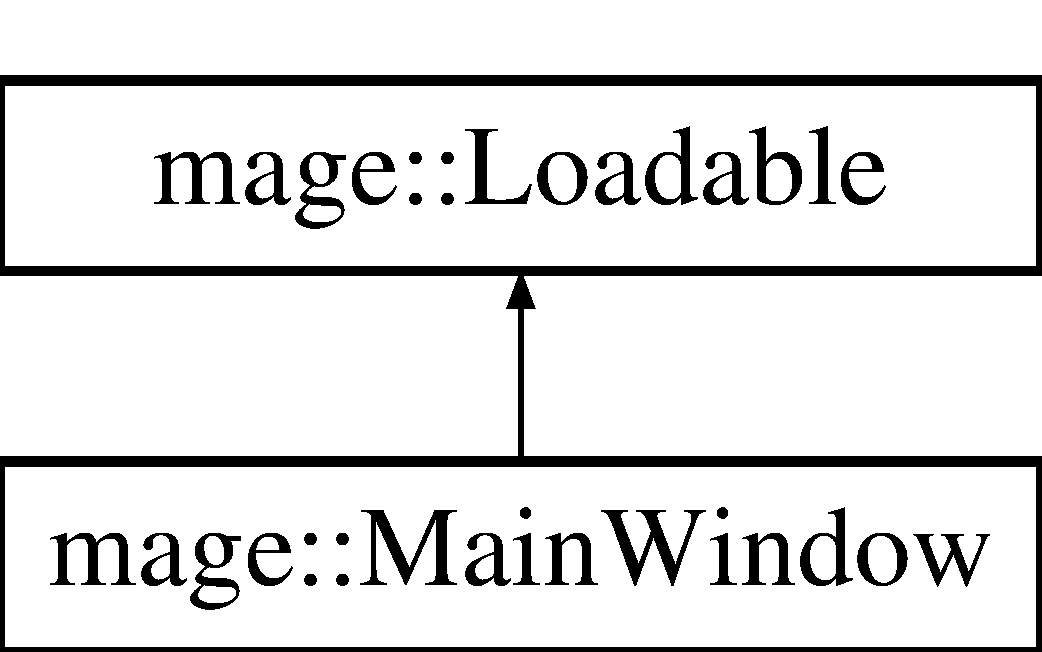
\includegraphics[height=2.000000cm]{classmage_1_1_main_window}
\end{center}
\end{figure}
\subsection*{Public Member Functions}
\begin{DoxyCompactItemize}
\item 
\hyperlink{classmage_1_1_main_window_a907a5c337e0e1f14281858b7713235ab}{Main\+Window} (H\+I\+N\+S\+T\+A\+N\+CE hinstance, const wstring \&name, L\+O\+NG width, L\+O\+NG height)
\item 
virtual \hyperlink{classmage_1_1_main_window_ada7ecf97d82ce08ba2f31f0afd891031}{$\sim$\+Main\+Window} ()
\item 
bool \hyperlink{classmage_1_1_main_window_aefa6d872bbe7702f51e4a0ca62ea587f}{Show} (int n\+Cmd\+Show)
\item 
H\+I\+N\+S\+T\+A\+N\+CE \hyperlink{classmage_1_1_main_window_ae26a7e1e96bc5522461aed6156138a0c}{Get\+Hinstance} () const
\item 
H\+W\+ND \hyperlink{classmage_1_1_main_window_acfaa88503f2c5e4a05aa9fa9698d2735}{Get\+Handle} () const
\item 
const wstring \& \hyperlink{classmage_1_1_main_window_aa2b99118a5125d4effbd5c5d9352e7e0}{Get\+Name} () const
\end{DoxyCompactItemize}
\subsection*{Private Member Functions}
\begin{DoxyCompactItemize}
\item 
\hyperlink{classmage_1_1_main_window_a8dc3c590bb168f8178a7db72ff60fd0c}{Main\+Window} (const \hyperlink{classmage_1_1_main_window}{Main\+Window} \&main\+\_\+window)=delete
\item 
\hyperlink{classmage_1_1_main_window}{Main\+Window} \& \hyperlink{classmage_1_1_main_window_a0c2414ae4e627fb401c045371c286de0}{operator=} (const \hyperlink{classmage_1_1_main_window}{Main\+Window} \&main\+\_\+window)=delete
\item 
H\+R\+E\+S\+U\+LT \hyperlink{classmage_1_1_main_window_a167b4c2771e6caa819045cf75f9bba5f}{Initialize\+Window} (L\+O\+NG width, L\+O\+NG height)
\item 
H\+R\+E\+S\+U\+LT \hyperlink{classmage_1_1_main_window_a74e01363d59c22597449edfc524a504e}{Initialize\+Window} (R\+E\+CT rectangle)
\item 
H\+R\+E\+S\+U\+LT \hyperlink{classmage_1_1_main_window_aa1ba43fc0a12ea43636fe0e62242a47d}{Uninitialize\+Window} ()
\end{DoxyCompactItemize}
\subsection*{Private Attributes}
\begin{DoxyCompactItemize}
\item 
H\+I\+N\+S\+T\+A\+N\+CE \hyperlink{classmage_1_1_main_window_a389348c5949b2cb464a8236bfcff00ef}{m\+\_\+hinstance}
\item 
H\+W\+ND \hyperlink{classmage_1_1_main_window_afc9afabcf8a52d79f02c8352451863cc}{m\+\_\+hwindow}
\item 
const wstring \hyperlink{classmage_1_1_main_window_a3d8eba5081df97c68b1f2aa7e5d5cb1c}{m\+\_\+name}
\end{DoxyCompactItemize}
\subsection*{Additional Inherited Members}


\subsection{Detailed Description}
A class of main windows. 

\subsection{Constructor \& Destructor Documentation}
\hypertarget{classmage_1_1_main_window_a907a5c337e0e1f14281858b7713235ab}{}\label{classmage_1_1_main_window_a907a5c337e0e1f14281858b7713235ab} 
\index{mage\+::\+Main\+Window@{mage\+::\+Main\+Window}!Main\+Window@{Main\+Window}}
\index{Main\+Window@{Main\+Window}!mage\+::\+Main\+Window@{mage\+::\+Main\+Window}}
\subsubsection{\texorpdfstring{Main\+Window()}{MainWindow()}\hspace{0.1cm}{\footnotesize\ttfamily [1/2]}}
{\footnotesize\ttfamily mage\+::\+Main\+Window\+::\+Main\+Window (\begin{DoxyParamCaption}\item[{H\+I\+N\+S\+T\+A\+N\+CE}]{hinstance,  }\item[{const wstring \&}]{name,  }\item[{L\+O\+NG}]{width,  }\item[{L\+O\+NG}]{height }\end{DoxyParamCaption})}

Constructs a main window.


\begin{DoxyParams}[1]{Parameters}
\mbox{\tt in}  & {\em hinstance} & The application instance handle. \\
\hline
\mbox{\tt in}  & {\em name} & A reference to the name of the application. \\
\hline
\mbox{\tt in}  & {\em width} & The width of the window. \\
\hline
\mbox{\tt in}  & {\em height} & The height of the window. \\
\hline
\end{DoxyParams}
\hypertarget{classmage_1_1_main_window_ada7ecf97d82ce08ba2f31f0afd891031}{}\label{classmage_1_1_main_window_ada7ecf97d82ce08ba2f31f0afd891031} 
\index{mage\+::\+Main\+Window@{mage\+::\+Main\+Window}!````~Main\+Window@{$\sim$\+Main\+Window}}
\index{````~Main\+Window@{$\sim$\+Main\+Window}!mage\+::\+Main\+Window@{mage\+::\+Main\+Window}}
\subsubsection{\texorpdfstring{$\sim$\+Main\+Window()}{~MainWindow()}}
{\footnotesize\ttfamily mage\+::\+Main\+Window\+::$\sim$\+Main\+Window (\begin{DoxyParamCaption}{ }\end{DoxyParamCaption})\hspace{0.3cm}{\ttfamily [virtual]}}

Destructs this main window. \hypertarget{classmage_1_1_main_window_a8dc3c590bb168f8178a7db72ff60fd0c}{}\label{classmage_1_1_main_window_a8dc3c590bb168f8178a7db72ff60fd0c} 
\index{mage\+::\+Main\+Window@{mage\+::\+Main\+Window}!Main\+Window@{Main\+Window}}
\index{Main\+Window@{Main\+Window}!mage\+::\+Main\+Window@{mage\+::\+Main\+Window}}
\subsubsection{\texorpdfstring{Main\+Window()}{MainWindow()}\hspace{0.1cm}{\footnotesize\ttfamily [2/2]}}
{\footnotesize\ttfamily mage\+::\+Main\+Window\+::\+Main\+Window (\begin{DoxyParamCaption}\item[{const \hyperlink{classmage_1_1_main_window}{Main\+Window} \&}]{main\+\_\+window }\end{DoxyParamCaption})\hspace{0.3cm}{\ttfamily [private]}, {\ttfamily [delete]}}

Constructs a main window from the given main window.


\begin{DoxyParams}[1]{Parameters}
\mbox{\tt in}  & {\em main\+\_\+window} & A reference to the main window. \\
\hline
\end{DoxyParams}


\subsection{Member Function Documentation}
\hypertarget{classmage_1_1_main_window_acfaa88503f2c5e4a05aa9fa9698d2735}{}\label{classmage_1_1_main_window_acfaa88503f2c5e4a05aa9fa9698d2735} 
\index{mage\+::\+Main\+Window@{mage\+::\+Main\+Window}!Get\+Handle@{Get\+Handle}}
\index{Get\+Handle@{Get\+Handle}!mage\+::\+Main\+Window@{mage\+::\+Main\+Window}}
\subsubsection{\texorpdfstring{Get\+Handle()}{GetHandle()}}
{\footnotesize\ttfamily H\+W\+ND mage\+::\+Main\+Window\+::\+Get\+Handle (\begin{DoxyParamCaption}{ }\end{DoxyParamCaption}) const}

Returns the window handle of this main window.

\begin{DoxyReturn}{Returns}
The window handle of this main window. 
\end{DoxyReturn}
\hypertarget{classmage_1_1_main_window_ae26a7e1e96bc5522461aed6156138a0c}{}\label{classmage_1_1_main_window_ae26a7e1e96bc5522461aed6156138a0c} 
\index{mage\+::\+Main\+Window@{mage\+::\+Main\+Window}!Get\+Hinstance@{Get\+Hinstance}}
\index{Get\+Hinstance@{Get\+Hinstance}!mage\+::\+Main\+Window@{mage\+::\+Main\+Window}}
\subsubsection{\texorpdfstring{Get\+Hinstance()}{GetHinstance()}}
{\footnotesize\ttfamily H\+I\+N\+S\+T\+A\+N\+CE mage\+::\+Main\+Window\+::\+Get\+Hinstance (\begin{DoxyParamCaption}{ }\end{DoxyParamCaption}) const}

Returns the application instance handle of this main window.

\begin{DoxyReturn}{Returns}
The application instance handle of this main window. 
\end{DoxyReturn}
\hypertarget{classmage_1_1_main_window_aa2b99118a5125d4effbd5c5d9352e7e0}{}\label{classmage_1_1_main_window_aa2b99118a5125d4effbd5c5d9352e7e0} 
\index{mage\+::\+Main\+Window@{mage\+::\+Main\+Window}!Get\+Name@{Get\+Name}}
\index{Get\+Name@{Get\+Name}!mage\+::\+Main\+Window@{mage\+::\+Main\+Window}}
\subsubsection{\texorpdfstring{Get\+Name()}{GetName()}}
{\footnotesize\ttfamily const wstring\& mage\+::\+Main\+Window\+::\+Get\+Name (\begin{DoxyParamCaption}{ }\end{DoxyParamCaption}) const}

Returns the name of this main window.

\begin{DoxyReturn}{Returns}
The name of this main window. 
\end{DoxyReturn}
\hypertarget{classmage_1_1_main_window_a167b4c2771e6caa819045cf75f9bba5f}{}\label{classmage_1_1_main_window_a167b4c2771e6caa819045cf75f9bba5f} 
\index{mage\+::\+Main\+Window@{mage\+::\+Main\+Window}!Initialize\+Window@{Initialize\+Window}}
\index{Initialize\+Window@{Initialize\+Window}!mage\+::\+Main\+Window@{mage\+::\+Main\+Window}}
\subsubsection{\texorpdfstring{Initialize\+Window()}{InitializeWindow()}\hspace{0.1cm}{\footnotesize\ttfamily [1/2]}}
{\footnotesize\ttfamily H\+R\+E\+S\+U\+LT mage\+::\+Main\+Window\+::\+Initialize\+Window (\begin{DoxyParamCaption}\item[{L\+O\+NG}]{width,  }\item[{L\+O\+NG}]{height }\end{DoxyParamCaption})\hspace{0.3cm}{\ttfamily [private]}}

Initializes the engine window of this main window.


\begin{DoxyParams}[1]{Parameters}
\mbox{\tt in}  & {\em width} & The width of the client rectangle of the window. \\
\hline
\mbox{\tt in}  & {\em height} & The height of the client rectangle of the window. \\
\hline
\end{DoxyParams}
\begin{DoxyReturn}{Returns}
A success/error value. 
\end{DoxyReturn}
\hypertarget{classmage_1_1_main_window_a74e01363d59c22597449edfc524a504e}{}\label{classmage_1_1_main_window_a74e01363d59c22597449edfc524a504e} 
\index{mage\+::\+Main\+Window@{mage\+::\+Main\+Window}!Initialize\+Window@{Initialize\+Window}}
\index{Initialize\+Window@{Initialize\+Window}!mage\+::\+Main\+Window@{mage\+::\+Main\+Window}}
\subsubsection{\texorpdfstring{Initialize\+Window()}{InitializeWindow()}\hspace{0.1cm}{\footnotesize\ttfamily [2/2]}}
{\footnotesize\ttfamily H\+R\+E\+S\+U\+LT mage\+::\+Main\+Window\+::\+Initialize\+Window (\begin{DoxyParamCaption}\item[{R\+E\+CT}]{rectangle }\end{DoxyParamCaption})\hspace{0.3cm}{\ttfamily [private]}}

Initializes the engine window of this main window.


\begin{DoxyParams}[1]{Parameters}
\mbox{\tt in}  & {\em rectangle} & The client rectangle of the window. \\
\hline
\end{DoxyParams}
\begin{DoxyReturn}{Returns}
A success/error value. 
\end{DoxyReturn}
\hypertarget{classmage_1_1_main_window_a0c2414ae4e627fb401c045371c286de0}{}\label{classmage_1_1_main_window_a0c2414ae4e627fb401c045371c286de0} 
\index{mage\+::\+Main\+Window@{mage\+::\+Main\+Window}!operator=@{operator=}}
\index{operator=@{operator=}!mage\+::\+Main\+Window@{mage\+::\+Main\+Window}}
\subsubsection{\texorpdfstring{operator=()}{operator=()}}
{\footnotesize\ttfamily \hyperlink{classmage_1_1_main_window}{Main\+Window}\& mage\+::\+Main\+Window\+::operator= (\begin{DoxyParamCaption}\item[{const \hyperlink{classmage_1_1_main_window}{Main\+Window} \&}]{main\+\_\+window }\end{DoxyParamCaption})\hspace{0.3cm}{\ttfamily [private]}, {\ttfamily [delete]}}

Copies the given main window to this main window.


\begin{DoxyParams}[1]{Parameters}
\mbox{\tt in}  & {\em main\+\_\+window} & A reference to the main window to copy from. \\
\hline
\end{DoxyParams}
\begin{DoxyReturn}{Returns}
A reference to the copy of the given main window (i.\+e. this main window). 
\end{DoxyReturn}
\hypertarget{classmage_1_1_main_window_aefa6d872bbe7702f51e4a0ca62ea587f}{}\label{classmage_1_1_main_window_aefa6d872bbe7702f51e4a0ca62ea587f} 
\index{mage\+::\+Main\+Window@{mage\+::\+Main\+Window}!Show@{Show}}
\index{Show@{Show}!mage\+::\+Main\+Window@{mage\+::\+Main\+Window}}
\subsubsection{\texorpdfstring{Show()}{Show()}}
{\footnotesize\ttfamily bool mage\+::\+Main\+Window\+::\+Show (\begin{DoxyParamCaption}\item[{int}]{n\+Cmd\+Show }\end{DoxyParamCaption})}

Sets the specified window\textquotesingle{}s show state of this main window.


\begin{DoxyParams}[1]{Parameters}
\mbox{\tt in}  & {\em n\+Cmd\+Show} & Controls how this window is to be shown. \\
\hline
\end{DoxyParams}
\begin{DoxyReturn}{Returns}
{\ttfamily true} if the window was previously visible. {\ttfamily false} otherwise. 
\end{DoxyReturn}
\hypertarget{classmage_1_1_main_window_aa1ba43fc0a12ea43636fe0e62242a47d}{}\label{classmage_1_1_main_window_aa1ba43fc0a12ea43636fe0e62242a47d} 
\index{mage\+::\+Main\+Window@{mage\+::\+Main\+Window}!Uninitialize\+Window@{Uninitialize\+Window}}
\index{Uninitialize\+Window@{Uninitialize\+Window}!mage\+::\+Main\+Window@{mage\+::\+Main\+Window}}
\subsubsection{\texorpdfstring{Uninitialize\+Window()}{UninitializeWindow()}}
{\footnotesize\ttfamily H\+R\+E\+S\+U\+LT mage\+::\+Main\+Window\+::\+Uninitialize\+Window (\begin{DoxyParamCaption}{ }\end{DoxyParamCaption})\hspace{0.3cm}{\ttfamily [private]}}

Unitializes the engine window of this main window.

\begin{DoxyReturn}{Returns}
A success/error value. 
\end{DoxyReturn}


\subsection{Member Data Documentation}
\hypertarget{classmage_1_1_main_window_a389348c5949b2cb464a8236bfcff00ef}{}\label{classmage_1_1_main_window_a389348c5949b2cb464a8236bfcff00ef} 
\index{mage\+::\+Main\+Window@{mage\+::\+Main\+Window}!m\+\_\+hinstance@{m\+\_\+hinstance}}
\index{m\+\_\+hinstance@{m\+\_\+hinstance}!mage\+::\+Main\+Window@{mage\+::\+Main\+Window}}
\subsubsection{\texorpdfstring{m\+\_\+hinstance}{m\_hinstance}}
{\footnotesize\ttfamily H\+I\+N\+S\+T\+A\+N\+CE mage\+::\+Main\+Window\+::m\+\_\+hinstance\hspace{0.3cm}{\ttfamily [private]}}

Application instance handle. \hypertarget{classmage_1_1_main_window_afc9afabcf8a52d79f02c8352451863cc}{}\label{classmage_1_1_main_window_afc9afabcf8a52d79f02c8352451863cc} 
\index{mage\+::\+Main\+Window@{mage\+::\+Main\+Window}!m\+\_\+hwindow@{m\+\_\+hwindow}}
\index{m\+\_\+hwindow@{m\+\_\+hwindow}!mage\+::\+Main\+Window@{mage\+::\+Main\+Window}}
\subsubsection{\texorpdfstring{m\+\_\+hwindow}{m\_hwindow}}
{\footnotesize\ttfamily H\+W\+ND mage\+::\+Main\+Window\+::m\+\_\+hwindow\hspace{0.3cm}{\ttfamily [private]}}

The handle of the parent window. \hypertarget{classmage_1_1_main_window_a3d8eba5081df97c68b1f2aa7e5d5cb1c}{}\label{classmage_1_1_main_window_a3d8eba5081df97c68b1f2aa7e5d5cb1c} 
\index{mage\+::\+Main\+Window@{mage\+::\+Main\+Window}!m\+\_\+name@{m\+\_\+name}}
\index{m\+\_\+name@{m\+\_\+name}!mage\+::\+Main\+Window@{mage\+::\+Main\+Window}}
\subsubsection{\texorpdfstring{m\+\_\+name}{m\_name}}
{\footnotesize\ttfamily const wstring mage\+::\+Main\+Window\+::m\+\_\+name\hspace{0.3cm}{\ttfamily [private]}}

The name of this main window. 
\hypertarget{classmage_1_1_memory_arena}{}\section{mage\+:\+:Memory\+Arena Class Reference}
\label{classmage_1_1_memory_arena}\index{mage\+::\+Memory\+Arena@{mage\+::\+Memory\+Arena}}


{\ttfamily \#include $<$memory\+\_\+arena.\+hpp$>$}

\subsection*{Public Member Functions}
\begin{DoxyCompactItemize}
\item 
\hyperlink{classmage_1_1_memory_arena_ac90beb8cf8dc42944a0fd6a4a9e8355c}{Memory\+Arena} (size\+\_\+t block\+\_\+size=32768)
\item 
virtual \hyperlink{classmage_1_1_memory_arena_a2bea1690184d21f54a4fb815a86e0c27}{$\sim$\+Memory\+Arena} ()
\item 
size\+\_\+t \hyperlink{classmage_1_1_memory_arena_a0db28bd286a517a30acdc061ace0bf56}{Get\+Block\+Size} () const
\item 
size\+\_\+t \hyperlink{classmage_1_1_memory_arena_a2789bf0c58dee881662bbb0c5ba73e55}{Get\+Current\+Block\+Size} () const
\item 
size\+\_\+t \hyperlink{classmage_1_1_memory_arena_ac4be7fb4d5623d6f78b1576c7884883a}{Get\+Total\+Block\+Size} () const
\item 
char $\ast$ \hyperlink{classmage_1_1_memory_arena_ac856206614ef9890d500df207d12e863}{Get\+Current\+Block\+Ptr} () const
\item 
void \hyperlink{classmage_1_1_memory_arena_a117b74c7bd5dfb28dfdaae6cab253491}{Reset} ()
\item 
void $\ast$ \hyperlink{classmage_1_1_memory_arena_a83f19bd85aea65001e6406075c105398}{Alloc} (size\+\_\+t size)
\item 
{\footnotesize template$<$typename T $>$ }\\T $\ast$ \hyperlink{classmage_1_1_memory_arena_ab249fe48cdf7c46f625050fe9583603a}{Alloc} (size\+\_\+t count=1, bool initialization=true)
\end{DoxyCompactItemize}
\subsection*{Protected Member Functions}
\begin{DoxyCompactItemize}
\item 
\hyperlink{classmage_1_1_memory_arena_a1eca6fdacbd1226f4b21f443d118168b}{Memory\+Arena} (const \hyperlink{classmage_1_1_memory_arena}{Memory\+Arena} \&arena)=delete
\item 
\hyperlink{classmage_1_1_memory_arena}{Memory\+Arena} \& \hyperlink{classmage_1_1_memory_arena_a7e7799f859c55435714933972ecb8b95}{operator=} (const \hyperlink{classmage_1_1_memory_arena}{Memory\+Arena} \&arena)=delete
\end{DoxyCompactItemize}
\subsection*{Protected Attributes}
\begin{DoxyCompactItemize}
\item 
const size\+\_\+t \hyperlink{classmage_1_1_memory_arena_a18177c245b045c5536330ffed284ed4d}{m\+\_\+block\+\_\+size}
\item 
size\+\_\+t \hyperlink{classmage_1_1_memory_arena_a880d07eb372ce1c8b907947fcbdfc59c}{m\+\_\+current\+\_\+block\+\_\+pos}
\item 
pair$<$ size\+\_\+t, char $\ast$$>$ \hyperlink{classmage_1_1_memory_arena_ab2d39233b1e64239baea519a2d073b04}{m\+\_\+current\+\_\+block}
\item 
list$<$ pair$<$ size\+\_\+t, char $\ast$$>$ $>$ \hyperlink{classmage_1_1_memory_arena_a9fc33bafde45afe06d05732572f415d1}{m\+\_\+used\+\_\+blocks}
\item 
list$<$ pair$<$ size\+\_\+t, char $\ast$$>$ $>$ \hyperlink{classmage_1_1_memory_arena_a89c4f1d2b4d5e05bb46fa303d70428c4}{m\+\_\+available\+\_\+blocks}
\end{DoxyCompactItemize}


\subsection{Detailed Description}
A class of memory arena\textquotesingle{}s. 

\subsection{Constructor \& Destructor Documentation}
\hypertarget{classmage_1_1_memory_arena_ac90beb8cf8dc42944a0fd6a4a9e8355c}{}\label{classmage_1_1_memory_arena_ac90beb8cf8dc42944a0fd6a4a9e8355c} 
\index{mage\+::\+Memory\+Arena@{mage\+::\+Memory\+Arena}!Memory\+Arena@{Memory\+Arena}}
\index{Memory\+Arena@{Memory\+Arena}!mage\+::\+Memory\+Arena@{mage\+::\+Memory\+Arena}}
\subsubsection{\texorpdfstring{Memory\+Arena()}{MemoryArena()}\hspace{0.1cm}{\footnotesize\ttfamily [1/2]}}
{\footnotesize\ttfamily mage\+::\+Memory\+Arena\+::\+Memory\+Arena (\begin{DoxyParamCaption}\item[{size\+\_\+t}]{block\+\_\+size = {\ttfamily 32768} }\end{DoxyParamCaption})}

Constructs a memory arena with given block size.


\begin{DoxyParams}[1]{Parameters}
\mbox{\tt in}  & {\em block\+\_\+size} & The maximum block size in bytes. \\
\hline
\end{DoxyParams}
\hypertarget{classmage_1_1_memory_arena_a2bea1690184d21f54a4fb815a86e0c27}{}\label{classmage_1_1_memory_arena_a2bea1690184d21f54a4fb815a86e0c27} 
\index{mage\+::\+Memory\+Arena@{mage\+::\+Memory\+Arena}!````~Memory\+Arena@{$\sim$\+Memory\+Arena}}
\index{````~Memory\+Arena@{$\sim$\+Memory\+Arena}!mage\+::\+Memory\+Arena@{mage\+::\+Memory\+Arena}}
\subsubsection{\texorpdfstring{$\sim$\+Memory\+Arena()}{~MemoryArena()}}
{\footnotesize\ttfamily virtual mage\+::\+Memory\+Arena\+::$\sim$\+Memory\+Arena (\begin{DoxyParamCaption}{ }\end{DoxyParamCaption})\hspace{0.3cm}{\ttfamily [virtual]}}

Destructs the given memory arena. \hypertarget{classmage_1_1_memory_arena_a1eca6fdacbd1226f4b21f443d118168b}{}\label{classmage_1_1_memory_arena_a1eca6fdacbd1226f4b21f443d118168b} 
\index{mage\+::\+Memory\+Arena@{mage\+::\+Memory\+Arena}!Memory\+Arena@{Memory\+Arena}}
\index{Memory\+Arena@{Memory\+Arena}!mage\+::\+Memory\+Arena@{mage\+::\+Memory\+Arena}}
\subsubsection{\texorpdfstring{Memory\+Arena()}{MemoryArena()}\hspace{0.1cm}{\footnotesize\ttfamily [2/2]}}
{\footnotesize\ttfamily mage\+::\+Memory\+Arena\+::\+Memory\+Arena (\begin{DoxyParamCaption}\item[{const \hyperlink{classmage_1_1_memory_arena}{Memory\+Arena} \&}]{arena }\end{DoxyParamCaption})\hspace{0.3cm}{\ttfamily [protected]}, {\ttfamily [delete]}}

Constructs a memory arena from the given memory arena.


\begin{DoxyParams}[1]{Parameters}
\mbox{\tt in}  & {\em arena} & The memory arena. \\
\hline
\end{DoxyParams}


\subsection{Member Function Documentation}
\hypertarget{classmage_1_1_memory_arena_a83f19bd85aea65001e6406075c105398}{}\label{classmage_1_1_memory_arena_a83f19bd85aea65001e6406075c105398} 
\index{mage\+::\+Memory\+Arena@{mage\+::\+Memory\+Arena}!Alloc@{Alloc}}
\index{Alloc@{Alloc}!mage\+::\+Memory\+Arena@{mage\+::\+Memory\+Arena}}
\subsubsection{\texorpdfstring{Alloc()}{Alloc()}\hspace{0.1cm}{\footnotesize\ttfamily [1/2]}}
{\footnotesize\ttfamily void$\ast$ mage\+::\+Memory\+Arena\+::\+Alloc (\begin{DoxyParamCaption}\item[{size\+\_\+t}]{size }\end{DoxyParamCaption})}

Allocates a block of memory of the given size.


\begin{DoxyParams}[1]{Parameters}
\mbox{\tt in}  & {\em size} & The requested size in bytes to allocate in memory. \\
\hline
\end{DoxyParams}
\begin{DoxyReturn}{Returns}
{\ttfamily nullptr} if the allocation failed. 

A pointer to the memory block that was allocated. 
\end{DoxyReturn}
\hypertarget{classmage_1_1_memory_arena_ab249fe48cdf7c46f625050fe9583603a}{}\label{classmage_1_1_memory_arena_ab249fe48cdf7c46f625050fe9583603a} 
\index{mage\+::\+Memory\+Arena@{mage\+::\+Memory\+Arena}!Alloc@{Alloc}}
\index{Alloc@{Alloc}!mage\+::\+Memory\+Arena@{mage\+::\+Memory\+Arena}}
\subsubsection{\texorpdfstring{Alloc()}{Alloc()}\hspace{0.1cm}{\footnotesize\ttfamily [2/2]}}
{\footnotesize\ttfamily template$<$typename T $>$ \\
T$\ast$ mage\+::\+Memory\+Arena\+::\+Alloc (\begin{DoxyParamCaption}\item[{size\+\_\+t}]{count = {\ttfamily 1},  }\item[{bool}]{initialization = {\ttfamily true} }\end{DoxyParamCaption})}

Allocates a block of memory.


\begin{DoxyTemplParams}{Template Parameters}
{\em T} & The type of objects to allocate in memory. \\
\hline
\end{DoxyTemplParams}

\begin{DoxyParams}[1]{Parameters}
\mbox{\tt in}  & {\em count} & The number of objects of type {\ttfamily T} to allocate in memory. \\
\hline
\mbox{\tt in}  & {\em initialization} & Flag indicating whether the objects need to be initialized (i.\+e. the constructor needs to be called). \\
\hline
\end{DoxyParams}
\begin{DoxyReturn}{Returns}
{\ttfamily nullptr} if the allocation failed. 

A pointer to the memory block that was allocated. 
\end{DoxyReturn}
\begin{DoxyNote}{Note}
The objects will be constructed with their default empty constructor. 
\end{DoxyNote}
\hypertarget{classmage_1_1_memory_arena_a0db28bd286a517a30acdc061ace0bf56}{}\label{classmage_1_1_memory_arena_a0db28bd286a517a30acdc061ace0bf56} 
\index{mage\+::\+Memory\+Arena@{mage\+::\+Memory\+Arena}!Get\+Block\+Size@{Get\+Block\+Size}}
\index{Get\+Block\+Size@{Get\+Block\+Size}!mage\+::\+Memory\+Arena@{mage\+::\+Memory\+Arena}}
\subsubsection{\texorpdfstring{Get\+Block\+Size()}{GetBlockSize()}}
{\footnotesize\ttfamily size\+\_\+t mage\+::\+Memory\+Arena\+::\+Get\+Block\+Size (\begin{DoxyParamCaption}{ }\end{DoxyParamCaption}) const}

Returns the maximum block size of this memory arena.

\begin{DoxyReturn}{Returns}
The maximum block size of this memory arena. 
\end{DoxyReturn}
\hypertarget{classmage_1_1_memory_arena_ac856206614ef9890d500df207d12e863}{}\label{classmage_1_1_memory_arena_ac856206614ef9890d500df207d12e863} 
\index{mage\+::\+Memory\+Arena@{mage\+::\+Memory\+Arena}!Get\+Current\+Block\+Ptr@{Get\+Current\+Block\+Ptr}}
\index{Get\+Current\+Block\+Ptr@{Get\+Current\+Block\+Ptr}!mage\+::\+Memory\+Arena@{mage\+::\+Memory\+Arena}}
\subsubsection{\texorpdfstring{Get\+Current\+Block\+Ptr()}{GetCurrentBlockPtr()}}
{\footnotesize\ttfamily char$\ast$ mage\+::\+Memory\+Arena\+::\+Get\+Current\+Block\+Ptr (\begin{DoxyParamCaption}{ }\end{DoxyParamCaption}) const}

Returns a pointer to the current block of this memory arena.

\begin{DoxyReturn}{Returns}
A pointer to the current block of this memory arena. 
\end{DoxyReturn}
\hypertarget{classmage_1_1_memory_arena_a2789bf0c58dee881662bbb0c5ba73e55}{}\label{classmage_1_1_memory_arena_a2789bf0c58dee881662bbb0c5ba73e55} 
\index{mage\+::\+Memory\+Arena@{mage\+::\+Memory\+Arena}!Get\+Current\+Block\+Size@{Get\+Current\+Block\+Size}}
\index{Get\+Current\+Block\+Size@{Get\+Current\+Block\+Size}!mage\+::\+Memory\+Arena@{mage\+::\+Memory\+Arena}}
\subsubsection{\texorpdfstring{Get\+Current\+Block\+Size()}{GetCurrentBlockSize()}}
{\footnotesize\ttfamily size\+\_\+t mage\+::\+Memory\+Arena\+::\+Get\+Current\+Block\+Size (\begin{DoxyParamCaption}{ }\end{DoxyParamCaption}) const}

Returns the block size (in bytes) of the current block of this memory arena.

\begin{DoxyReturn}{Returns}
The block size (in bytes) of the current block of this memory arena. 
\end{DoxyReturn}
\hypertarget{classmage_1_1_memory_arena_ac4be7fb4d5623d6f78b1576c7884883a}{}\label{classmage_1_1_memory_arena_ac4be7fb4d5623d6f78b1576c7884883a} 
\index{mage\+::\+Memory\+Arena@{mage\+::\+Memory\+Arena}!Get\+Total\+Block\+Size@{Get\+Total\+Block\+Size}}
\index{Get\+Total\+Block\+Size@{Get\+Total\+Block\+Size}!mage\+::\+Memory\+Arena@{mage\+::\+Memory\+Arena}}
\subsubsection{\texorpdfstring{Get\+Total\+Block\+Size()}{GetTotalBlockSize()}}
{\footnotesize\ttfamily size\+\_\+t mage\+::\+Memory\+Arena\+::\+Get\+Total\+Block\+Size (\begin{DoxyParamCaption}{ }\end{DoxyParamCaption}) const}

Returns the block size (in bytes) of all blocks of this memory arena.

\begin{DoxyReturn}{Returns}
The block size (in bytes) of all blocks of this memory arena. 
\end{DoxyReturn}
\hypertarget{classmage_1_1_memory_arena_a7e7799f859c55435714933972ecb8b95}{}\label{classmage_1_1_memory_arena_a7e7799f859c55435714933972ecb8b95} 
\index{mage\+::\+Memory\+Arena@{mage\+::\+Memory\+Arena}!operator=@{operator=}}
\index{operator=@{operator=}!mage\+::\+Memory\+Arena@{mage\+::\+Memory\+Arena}}
\subsubsection{\texorpdfstring{operator=()}{operator=()}}
{\footnotesize\ttfamily \hyperlink{classmage_1_1_memory_arena}{Memory\+Arena}\& mage\+::\+Memory\+Arena\+::operator= (\begin{DoxyParamCaption}\item[{const \hyperlink{classmage_1_1_memory_arena}{Memory\+Arena} \&}]{arena }\end{DoxyParamCaption})\hspace{0.3cm}{\ttfamily [protected]}, {\ttfamily [delete]}}

Copies the given memory arena to this memory arena.


\begin{DoxyParams}[1]{Parameters}
\mbox{\tt in}  & {\em arena} & The memory arena. \\
\hline
\end{DoxyParams}
\hypertarget{classmage_1_1_memory_arena_a117b74c7bd5dfb28dfdaae6cab253491}{}\label{classmage_1_1_memory_arena_a117b74c7bd5dfb28dfdaae6cab253491} 
\index{mage\+::\+Memory\+Arena@{mage\+::\+Memory\+Arena}!Reset@{Reset}}
\index{Reset@{Reset}!mage\+::\+Memory\+Arena@{mage\+::\+Memory\+Arena}}
\subsubsection{\texorpdfstring{Reset()}{Reset()}}
{\footnotesize\ttfamily void mage\+::\+Memory\+Arena\+::\+Reset (\begin{DoxyParamCaption}{ }\end{DoxyParamCaption})}

Resets this memory arena. 

\subsection{Member Data Documentation}
\hypertarget{classmage_1_1_memory_arena_a89c4f1d2b4d5e05bb46fa303d70428c4}{}\label{classmage_1_1_memory_arena_a89c4f1d2b4d5e05bb46fa303d70428c4} 
\index{mage\+::\+Memory\+Arena@{mage\+::\+Memory\+Arena}!m\+\_\+available\+\_\+blocks@{m\+\_\+available\+\_\+blocks}}
\index{m\+\_\+available\+\_\+blocks@{m\+\_\+available\+\_\+blocks}!mage\+::\+Memory\+Arena@{mage\+::\+Memory\+Arena}}
\subsubsection{\texorpdfstring{m\+\_\+available\+\_\+blocks}{m\_available\_blocks}}
{\footnotesize\ttfamily list$<$ pair$<$ size\+\_\+t, char $\ast$ $>$ $>$ mage\+::\+Memory\+Arena\+::m\+\_\+available\+\_\+blocks\hspace{0.3cm}{\ttfamily [protected]}}

Pointers to the available blocks of this memory arena. \hypertarget{classmage_1_1_memory_arena_a18177c245b045c5536330ffed284ed4d}{}\label{classmage_1_1_memory_arena_a18177c245b045c5536330ffed284ed4d} 
\index{mage\+::\+Memory\+Arena@{mage\+::\+Memory\+Arena}!m\+\_\+block\+\_\+size@{m\+\_\+block\+\_\+size}}
\index{m\+\_\+block\+\_\+size@{m\+\_\+block\+\_\+size}!mage\+::\+Memory\+Arena@{mage\+::\+Memory\+Arena}}
\subsubsection{\texorpdfstring{m\+\_\+block\+\_\+size}{m\_block\_size}}
{\footnotesize\ttfamily const size\+\_\+t mage\+::\+Memory\+Arena\+::m\+\_\+block\+\_\+size\hspace{0.3cm}{\ttfamily [protected]}}

The fixed block size of this memory arena. \hypertarget{classmage_1_1_memory_arena_ab2d39233b1e64239baea519a2d073b04}{}\label{classmage_1_1_memory_arena_ab2d39233b1e64239baea519a2d073b04} 
\index{mage\+::\+Memory\+Arena@{mage\+::\+Memory\+Arena}!m\+\_\+current\+\_\+block@{m\+\_\+current\+\_\+block}}
\index{m\+\_\+current\+\_\+block@{m\+\_\+current\+\_\+block}!mage\+::\+Memory\+Arena@{mage\+::\+Memory\+Arena}}
\subsubsection{\texorpdfstring{m\+\_\+current\+\_\+block}{m\_current\_block}}
{\footnotesize\ttfamily pair$<$ size\+\_\+t, char $\ast$ $>$ mage\+::\+Memory\+Arena\+::m\+\_\+current\+\_\+block\hspace{0.3cm}{\ttfamily [protected]}}

A pointer to the current block of this memory arena. \hypertarget{classmage_1_1_memory_arena_a880d07eb372ce1c8b907947fcbdfc59c}{}\label{classmage_1_1_memory_arena_a880d07eb372ce1c8b907947fcbdfc59c} 
\index{mage\+::\+Memory\+Arena@{mage\+::\+Memory\+Arena}!m\+\_\+current\+\_\+block\+\_\+pos@{m\+\_\+current\+\_\+block\+\_\+pos}}
\index{m\+\_\+current\+\_\+block\+\_\+pos@{m\+\_\+current\+\_\+block\+\_\+pos}!mage\+::\+Memory\+Arena@{mage\+::\+Memory\+Arena}}
\subsubsection{\texorpdfstring{m\+\_\+current\+\_\+block\+\_\+pos}{m\_current\_block\_pos}}
{\footnotesize\ttfamily size\+\_\+t mage\+::\+Memory\+Arena\+::m\+\_\+current\+\_\+block\+\_\+pos\hspace{0.3cm}{\ttfamily [protected]}}

The current block position of this memory arena. \hypertarget{classmage_1_1_memory_arena_a9fc33bafde45afe06d05732572f415d1}{}\label{classmage_1_1_memory_arena_a9fc33bafde45afe06d05732572f415d1} 
\index{mage\+::\+Memory\+Arena@{mage\+::\+Memory\+Arena}!m\+\_\+used\+\_\+blocks@{m\+\_\+used\+\_\+blocks}}
\index{m\+\_\+used\+\_\+blocks@{m\+\_\+used\+\_\+blocks}!mage\+::\+Memory\+Arena@{mage\+::\+Memory\+Arena}}
\subsubsection{\texorpdfstring{m\+\_\+used\+\_\+blocks}{m\_used\_blocks}}
{\footnotesize\ttfamily list$<$ pair$<$ size\+\_\+t, char $\ast$ $>$ $>$ mage\+::\+Memory\+Arena\+::m\+\_\+used\+\_\+blocks\hspace{0.3cm}{\ttfamily [protected]}}

Pointers to the used blocks of this memory arena. 
\hypertarget{classmage_1_1_mouse}{}\section{mage\+:\+:Mouse Class Reference}
\label{classmage_1_1_mouse}\index{mage\+::\+Mouse@{mage\+::\+Mouse}}


{\ttfamily \#include $<$mouse.\+hpp$>$}

Inheritance diagram for mage\+:\+:Mouse\+:\begin{figure}[H]
\begin{center}
\leavevmode
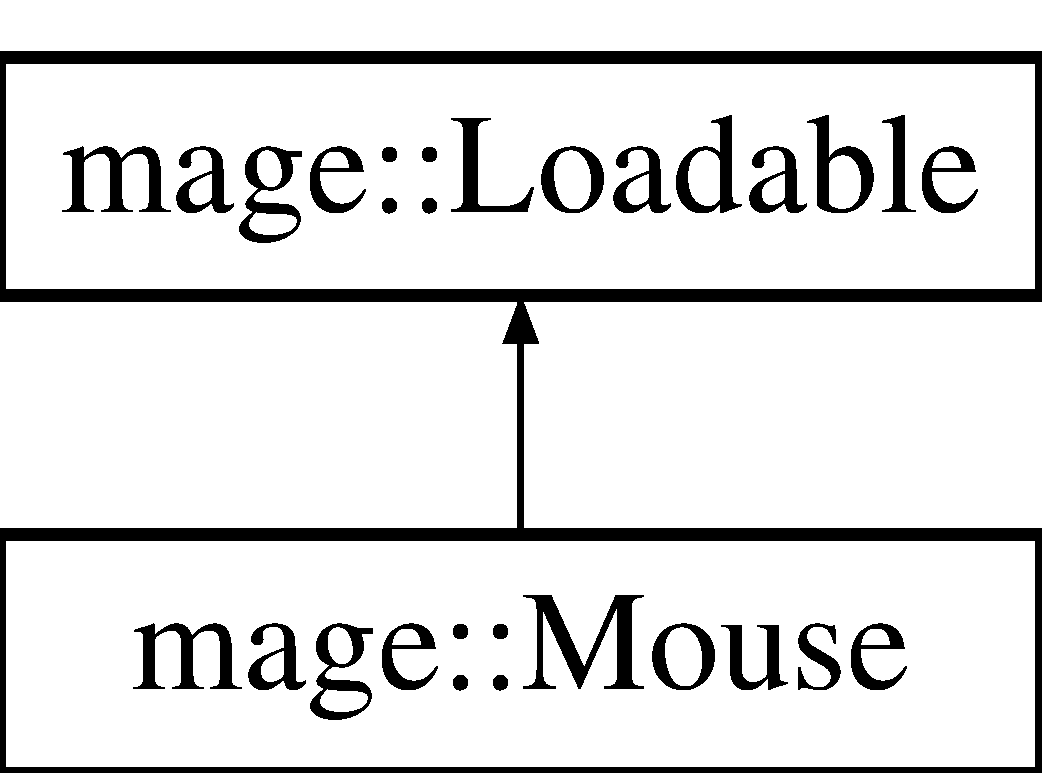
\includegraphics[height=2.000000cm]{classmage_1_1_mouse}
\end{center}
\end{figure}
\subsection*{Public Member Functions}
\begin{DoxyCompactItemize}
\item 
\hyperlink{classmage_1_1_mouse_af7a493eeef5b370eb390ccbfc7eed673}{Mouse} (H\+W\+ND hwindow, \hyperlink{namespacemage_ae74f374780900893caa5555d1031fd79}{Com\+Ptr}$<$ I\+Direct\+Input8 $>$ di)
\item 
virtual \hyperlink{classmage_1_1_mouse_a6ff5841bae697af04496dbf6e645b4b9}{$\sim$\+Mouse} ()
\item 
void \hyperlink{classmage_1_1_mouse_a0cddae3f871dd69c1ba6928dc6b1f985}{Update} ()
\item 
H\+W\+ND \hyperlink{classmage_1_1_mouse_afd77480c5b2c9873b8c1ac2d3a9a7c73}{Get\+Handle} () const
\item 
bool \hyperlink{classmage_1_1_mouse_a9c8d4493c86685b259819b5995a17c7a}{Get\+Mouse\+Button\+Press} (char mouse\+\_\+button, bool ignore\+\_\+press\+\_\+stamp=false) const
\item 
long \hyperlink{classmage_1_1_mouse_a6af2e1ea96554ee34e16a37a257fe11c}{Get\+PosX} () const
\item 
long \hyperlink{classmage_1_1_mouse_af4da58c811896f0814956382a756db61}{Get\+PosY} () const
\item 
long \hyperlink{classmage_1_1_mouse_a137313b065314d98c7b61eaefce6c3d1}{Get\+DeltaX} () const
\item 
long \hyperlink{classmage_1_1_mouse_af0769d0f7658b0699cf5b4f797163510}{Get\+DeltaY} () const
\item 
long \hyperlink{classmage_1_1_mouse_a898f4d0e645040c3a4121c2fe8119a89}{Get\+Delta\+Wheel} () const
\end{DoxyCompactItemize}
\subsection*{Protected Member Functions}
\begin{DoxyCompactItemize}
\item 
H\+R\+E\+S\+U\+LT \hyperlink{classmage_1_1_mouse_a22d790c9c31ca62d595637983b6da940}{Initialize\+Mouse} (\hyperlink{namespacemage_ae74f374780900893caa5555d1031fd79}{Com\+Ptr}$<$ I\+Direct\+Input8 $>$ di)
\end{DoxyCompactItemize}
\subsection*{Protected Attributes}
\begin{DoxyCompactItemize}
\item 
uint64\+\_\+t \hyperlink{classmage_1_1_mouse_a32b30d3c37a2082869f4ff4f522dfbf8}{m\+\_\+press\+\_\+stamp}
\item 
\hyperlink{namespacemage_ae74f374780900893caa5555d1031fd79}{Com\+Ptr}$<$ I\+Direct\+Input\+Device8 $>$ \hyperlink{classmage_1_1_mouse_a3f2803f3c0e008f5d764a11de3dbe098}{m\+\_\+mouse}
\item 
D\+I\+M\+O\+U\+S\+E\+S\+T\+A\+TE \hyperlink{classmage_1_1_mouse_af99645fb4226077abee4532a5e663066}{m\+\_\+mouse\+\_\+state}
\item 
uint64\+\_\+t \hyperlink{classmage_1_1_mouse_a0f5a38e23bdf7eae1b7b1030a53edff0}{m\+\_\+mouse\+\_\+button\+\_\+press\+\_\+stamp} \mbox{[}3\mbox{]}
\item 
P\+O\+I\+NT \hyperlink{classmage_1_1_mouse_a2a8332ef7a4daa0f9ed48a9a1ad80684}{m\+\_\+mouse\+\_\+position}
\end{DoxyCompactItemize}
\subsection*{Private Member Functions}
\begin{DoxyCompactItemize}
\item 
\hyperlink{classmage_1_1_mouse_af11aa23e6cfbefb4cd3d90b17c63db7c}{Mouse} (const \hyperlink{classmage_1_1_mouse}{Mouse} \&mouse)=delete
\item 
\hyperlink{classmage_1_1_mouse}{Mouse} \& \hyperlink{classmage_1_1_mouse_a585119f1b0db3fbc7436c86676518c8c}{operator=} (const \hyperlink{classmage_1_1_mouse}{Mouse} \&mouse)=delete
\end{DoxyCompactItemize}
\subsection*{Private Attributes}
\begin{DoxyCompactItemize}
\item 
H\+W\+ND \hyperlink{classmage_1_1_mouse_a0c67906df7b8b0cce013c724be4625ac}{m\+\_\+hwindow}
\end{DoxyCompactItemize}


\subsection{Detailed Description}
A class of mouses. 

\subsection{Constructor \& Destructor Documentation}
\hypertarget{classmage_1_1_mouse_af7a493eeef5b370eb390ccbfc7eed673}{}\label{classmage_1_1_mouse_af7a493eeef5b370eb390ccbfc7eed673} 
\index{mage\+::\+Mouse@{mage\+::\+Mouse}!Mouse@{Mouse}}
\index{Mouse@{Mouse}!mage\+::\+Mouse@{mage\+::\+Mouse}}
\subsubsection{\texorpdfstring{Mouse()}{Mouse()}\hspace{0.1cm}{\footnotesize\ttfamily [1/2]}}
{\footnotesize\ttfamily mage\+::\+Mouse\+::\+Mouse (\begin{DoxyParamCaption}\item[{H\+W\+ND}]{hwindow,  }\item[{\hyperlink{namespacemage_ae74f374780900893caa5555d1031fd79}{Com\+Ptr}$<$ I\+Direct\+Input8 $>$}]{di }\end{DoxyParamCaption})}

Constructs a mouse.


\begin{DoxyParams}[1]{Parameters}
\mbox{\tt in}  & {\em hwindow} & The handle of the parent window. \\
\hline
\mbox{\tt in}  & {\em di} & A pointer to a direct input object. \\
\hline
\end{DoxyParams}
\hypertarget{classmage_1_1_mouse_a6ff5841bae697af04496dbf6e645b4b9}{}\label{classmage_1_1_mouse_a6ff5841bae697af04496dbf6e645b4b9} 
\index{mage\+::\+Mouse@{mage\+::\+Mouse}!````~Mouse@{$\sim$\+Mouse}}
\index{````~Mouse@{$\sim$\+Mouse}!mage\+::\+Mouse@{mage\+::\+Mouse}}
\subsubsection{\texorpdfstring{$\sim$\+Mouse()}{~Mouse()}}
{\footnotesize\ttfamily virtual mage\+::\+Mouse\+::$\sim$\+Mouse (\begin{DoxyParamCaption}{ }\end{DoxyParamCaption})\hspace{0.3cm}{\ttfamily [virtual]}}

Destructs this mouse. \hypertarget{classmage_1_1_mouse_af11aa23e6cfbefb4cd3d90b17c63db7c}{}\label{classmage_1_1_mouse_af11aa23e6cfbefb4cd3d90b17c63db7c} 
\index{mage\+::\+Mouse@{mage\+::\+Mouse}!Mouse@{Mouse}}
\index{Mouse@{Mouse}!mage\+::\+Mouse@{mage\+::\+Mouse}}
\subsubsection{\texorpdfstring{Mouse()}{Mouse()}\hspace{0.1cm}{\footnotesize\ttfamily [2/2]}}
{\footnotesize\ttfamily mage\+::\+Mouse\+::\+Mouse (\begin{DoxyParamCaption}\item[{const \hyperlink{classmage_1_1_mouse}{Mouse} \&}]{mouse }\end{DoxyParamCaption})\hspace{0.3cm}{\ttfamily [private]}, {\ttfamily [delete]}}

Constructs a mouse from the given mouse.


\begin{DoxyParams}[1]{Parameters}
\mbox{\tt in}  & {\em mouse} & A reference to the mouse. \\
\hline
\end{DoxyParams}


\subsection{Member Function Documentation}
\hypertarget{classmage_1_1_mouse_a898f4d0e645040c3a4121c2fe8119a89}{}\label{classmage_1_1_mouse_a898f4d0e645040c3a4121c2fe8119a89} 
\index{mage\+::\+Mouse@{mage\+::\+Mouse}!Get\+Delta\+Wheel@{Get\+Delta\+Wheel}}
\index{Get\+Delta\+Wheel@{Get\+Delta\+Wheel}!mage\+::\+Mouse@{mage\+::\+Mouse}}
\subsubsection{\texorpdfstring{Get\+Delta\+Wheel()}{GetDeltaWheel()}}
{\footnotesize\ttfamily long mage\+::\+Mouse\+::\+Get\+Delta\+Wheel (\begin{DoxyParamCaption}{ }\end{DoxyParamCaption}) const}

Returns the change in this mouse\textquotesingle{}s scroll wheel.

\begin{DoxyReturn}{Returns}
The change in this mouse\textquotesingle{}s scroll wheel. 
\end{DoxyReturn}
\hypertarget{classmage_1_1_mouse_a137313b065314d98c7b61eaefce6c3d1}{}\label{classmage_1_1_mouse_a137313b065314d98c7b61eaefce6c3d1} 
\index{mage\+::\+Mouse@{mage\+::\+Mouse}!Get\+DeltaX@{Get\+DeltaX}}
\index{Get\+DeltaX@{Get\+DeltaX}!mage\+::\+Mouse@{mage\+::\+Mouse}}
\subsubsection{\texorpdfstring{Get\+Delta\+X()}{GetDeltaX()}}
{\footnotesize\ttfamily long mage\+::\+Mouse\+::\+Get\+DeltaX (\begin{DoxyParamCaption}{ }\end{DoxyParamCaption}) const}

Returns the change in this mouse\textquotesingle{}s horizontal coordinate.

\begin{DoxyReturn}{Returns}
The change in this mouse\textquotesingle{}s horizontal coordinate. 
\end{DoxyReturn}
\hypertarget{classmage_1_1_mouse_af0769d0f7658b0699cf5b4f797163510}{}\label{classmage_1_1_mouse_af0769d0f7658b0699cf5b4f797163510} 
\index{mage\+::\+Mouse@{mage\+::\+Mouse}!Get\+DeltaY@{Get\+DeltaY}}
\index{Get\+DeltaY@{Get\+DeltaY}!mage\+::\+Mouse@{mage\+::\+Mouse}}
\subsubsection{\texorpdfstring{Get\+Delta\+Y()}{GetDeltaY()}}
{\footnotesize\ttfamily long mage\+::\+Mouse\+::\+Get\+DeltaY (\begin{DoxyParamCaption}{ }\end{DoxyParamCaption}) const}

Returns the change in this mouse\textquotesingle{}s vertical coordinate.

\begin{DoxyReturn}{Returns}
The change in this mouse\textquotesingle{}s vertical coordinate. 
\end{DoxyReturn}
\hypertarget{classmage_1_1_mouse_afd77480c5b2c9873b8c1ac2d3a9a7c73}{}\label{classmage_1_1_mouse_afd77480c5b2c9873b8c1ac2d3a9a7c73} 
\index{mage\+::\+Mouse@{mage\+::\+Mouse}!Get\+Handle@{Get\+Handle}}
\index{Get\+Handle@{Get\+Handle}!mage\+::\+Mouse@{mage\+::\+Mouse}}
\subsubsection{\texorpdfstring{Get\+Handle()}{GetHandle()}}
{\footnotesize\ttfamily H\+W\+ND mage\+::\+Mouse\+::\+Get\+Handle (\begin{DoxyParamCaption}{ }\end{DoxyParamCaption}) const}

Returns the window handle of this mouse.

\begin{DoxyReturn}{Returns}
The window handle of this mouse. 
\end{DoxyReturn}
\hypertarget{classmage_1_1_mouse_a9c8d4493c86685b259819b5995a17c7a}{}\label{classmage_1_1_mouse_a9c8d4493c86685b259819b5995a17c7a} 
\index{mage\+::\+Mouse@{mage\+::\+Mouse}!Get\+Mouse\+Button\+Press@{Get\+Mouse\+Button\+Press}}
\index{Get\+Mouse\+Button\+Press@{Get\+Mouse\+Button\+Press}!mage\+::\+Mouse@{mage\+::\+Mouse}}
\subsubsection{\texorpdfstring{Get\+Mouse\+Button\+Press()}{GetMouseButtonPress()}}
{\footnotesize\ttfamily bool mage\+::\+Mouse\+::\+Get\+Mouse\+Button\+Press (\begin{DoxyParamCaption}\item[{char}]{mouse\+\_\+button,  }\item[{bool}]{ignore\+\_\+press\+\_\+stamp = {\ttfamily false} }\end{DoxyParamCaption}) const}

Checks whether the given mouse button of this mouse is pressed.


\begin{DoxyParams}[1]{Parameters}
\mbox{\tt in}  & {\em mouse\+\_\+button} & The mouse button. \\
\hline
\mbox{\tt in}  & {\em ignore\+\_\+press\+\_\+stamp} & Flag indicating whether press stamps should be ignored. Consistent presses will return false when using the press stamp. \\
\hline
\end{DoxyParams}
\begin{DoxyReturn}{Returns}
{\ttfamily true} if the given mouse button is pressed. {\ttfamily false} otherwise. 
\end{DoxyReturn}
\hypertarget{classmage_1_1_mouse_a6af2e1ea96554ee34e16a37a257fe11c}{}\label{classmage_1_1_mouse_a6af2e1ea96554ee34e16a37a257fe11c} 
\index{mage\+::\+Mouse@{mage\+::\+Mouse}!Get\+PosX@{Get\+PosX}}
\index{Get\+PosX@{Get\+PosX}!mage\+::\+Mouse@{mage\+::\+Mouse}}
\subsubsection{\texorpdfstring{Get\+Pos\+X()}{GetPosX()}}
{\footnotesize\ttfamily long mage\+::\+Mouse\+::\+Get\+PosX (\begin{DoxyParamCaption}{ }\end{DoxyParamCaption}) const}

Returns the horizontal position of this mouse.

\begin{DoxyReturn}{Returns}
The horizontal position of this mouse. 
\end{DoxyReturn}
\hypertarget{classmage_1_1_mouse_af4da58c811896f0814956382a756db61}{}\label{classmage_1_1_mouse_af4da58c811896f0814956382a756db61} 
\index{mage\+::\+Mouse@{mage\+::\+Mouse}!Get\+PosY@{Get\+PosY}}
\index{Get\+PosY@{Get\+PosY}!mage\+::\+Mouse@{mage\+::\+Mouse}}
\subsubsection{\texorpdfstring{Get\+Pos\+Y()}{GetPosY()}}
{\footnotesize\ttfamily long mage\+::\+Mouse\+::\+Get\+PosY (\begin{DoxyParamCaption}{ }\end{DoxyParamCaption}) const}

Returns the vertical position of this mouse.

\begin{DoxyReturn}{Returns}
The vertical position of this mouse. 
\end{DoxyReturn}
\hypertarget{classmage_1_1_mouse_a22d790c9c31ca62d595637983b6da940}{}\label{classmage_1_1_mouse_a22d790c9c31ca62d595637983b6da940} 
\index{mage\+::\+Mouse@{mage\+::\+Mouse}!Initialize\+Mouse@{Initialize\+Mouse}}
\index{Initialize\+Mouse@{Initialize\+Mouse}!mage\+::\+Mouse@{mage\+::\+Mouse}}
\subsubsection{\texorpdfstring{Initialize\+Mouse()}{InitializeMouse()}}
{\footnotesize\ttfamily H\+R\+E\+S\+U\+LT mage\+::\+Mouse\+::\+Initialize\+Mouse (\begin{DoxyParamCaption}\item[{\hyperlink{namespacemage_ae74f374780900893caa5555d1031fd79}{Com\+Ptr}$<$ I\+Direct\+Input8 $>$}]{di }\end{DoxyParamCaption})\hspace{0.3cm}{\ttfamily [protected]}}

Initializes the mouse device of this mouse.


\begin{DoxyParams}[1]{Parameters}
\mbox{\tt in}  & {\em di} & A pointer to a direct input object. \\
\hline
\end{DoxyParams}
\begin{DoxyReturn}{Returns}
A success/error value. 
\end{DoxyReturn}
\hypertarget{classmage_1_1_mouse_a585119f1b0db3fbc7436c86676518c8c}{}\label{classmage_1_1_mouse_a585119f1b0db3fbc7436c86676518c8c} 
\index{mage\+::\+Mouse@{mage\+::\+Mouse}!operator=@{operator=}}
\index{operator=@{operator=}!mage\+::\+Mouse@{mage\+::\+Mouse}}
\subsubsection{\texorpdfstring{operator=()}{operator=()}}
{\footnotesize\ttfamily \hyperlink{classmage_1_1_mouse}{Mouse}\& mage\+::\+Mouse\+::operator= (\begin{DoxyParamCaption}\item[{const \hyperlink{classmage_1_1_mouse}{Mouse} \&}]{mouse }\end{DoxyParamCaption})\hspace{0.3cm}{\ttfamily [private]}, {\ttfamily [delete]}}

Copies the given mouse to this mouse.


\begin{DoxyParams}[1]{Parameters}
\mbox{\tt in}  & {\em mouse} & A reference to the mouse to copy from. \\
\hline
\end{DoxyParams}
\begin{DoxyReturn}{Returns}
A reference to the copy of the given mouse (i.\+e. this mouse). 
\end{DoxyReturn}
\hypertarget{classmage_1_1_mouse_a0cddae3f871dd69c1ba6928dc6b1f985}{}\label{classmage_1_1_mouse_a0cddae3f871dd69c1ba6928dc6b1f985} 
\index{mage\+::\+Mouse@{mage\+::\+Mouse}!Update@{Update}}
\index{Update@{Update}!mage\+::\+Mouse@{mage\+::\+Mouse}}
\subsubsection{\texorpdfstring{Update()}{Update()}}
{\footnotesize\ttfamily void mage\+::\+Mouse\+::\+Update (\begin{DoxyParamCaption}{ }\end{DoxyParamCaption})}

Updates the state of this mouse. 

\subsection{Member Data Documentation}
\hypertarget{classmage_1_1_mouse_a0c67906df7b8b0cce013c724be4625ac}{}\label{classmage_1_1_mouse_a0c67906df7b8b0cce013c724be4625ac} 
\index{mage\+::\+Mouse@{mage\+::\+Mouse}!m\+\_\+hwindow@{m\+\_\+hwindow}}
\index{m\+\_\+hwindow@{m\+\_\+hwindow}!mage\+::\+Mouse@{mage\+::\+Mouse}}
\subsubsection{\texorpdfstring{m\+\_\+hwindow}{m\_hwindow}}
{\footnotesize\ttfamily H\+W\+ND mage\+::\+Mouse\+::m\+\_\+hwindow\hspace{0.3cm}{\ttfamily [private]}}

The handle of the parent window. \hypertarget{classmage_1_1_mouse_a3f2803f3c0e008f5d764a11de3dbe098}{}\label{classmage_1_1_mouse_a3f2803f3c0e008f5d764a11de3dbe098} 
\index{mage\+::\+Mouse@{mage\+::\+Mouse}!m\+\_\+mouse@{m\+\_\+mouse}}
\index{m\+\_\+mouse@{m\+\_\+mouse}!mage\+::\+Mouse@{mage\+::\+Mouse}}
\subsubsection{\texorpdfstring{m\+\_\+mouse}{m\_mouse}}
{\footnotesize\ttfamily \hyperlink{namespacemage_ae74f374780900893caa5555d1031fd79}{Com\+Ptr}$<$ I\+Direct\+Input\+Device8 $>$ mage\+::\+Mouse\+::m\+\_\+mouse\hspace{0.3cm}{\ttfamily [protected]}}

Direct\+Input mouse device of this mouse.

The methods of the I\+Direct\+Input\+Device8 interface are used to gain and release access to Microsoft Direct\+Input devices, manage device properties and information, set behavior, perform initialization, create and play force-\/feedback effects, and invoke a device\textquotesingle{}s control panel. \hypertarget{classmage_1_1_mouse_a0f5a38e23bdf7eae1b7b1030a53edff0}{}\label{classmage_1_1_mouse_a0f5a38e23bdf7eae1b7b1030a53edff0} 
\index{mage\+::\+Mouse@{mage\+::\+Mouse}!m\+\_\+mouse\+\_\+button\+\_\+press\+\_\+stamp@{m\+\_\+mouse\+\_\+button\+\_\+press\+\_\+stamp}}
\index{m\+\_\+mouse\+\_\+button\+\_\+press\+\_\+stamp@{m\+\_\+mouse\+\_\+button\+\_\+press\+\_\+stamp}!mage\+::\+Mouse@{mage\+::\+Mouse}}
\subsubsection{\texorpdfstring{m\+\_\+mouse\+\_\+button\+\_\+press\+\_\+stamp}{m\_mouse\_button\_press\_stamp}}
{\footnotesize\ttfamily uint64\+\_\+t mage\+::\+Mouse\+::m\+\_\+mouse\+\_\+button\+\_\+press\+\_\+stamp\mbox{[}3\mbox{]}\hspace{0.3cm}{\ttfamily [mutable]}, {\ttfamily [protected]}}

Stamps the mouse buttons pressed in the last frame of this mouse. \hypertarget{classmage_1_1_mouse_a2a8332ef7a4daa0f9ed48a9a1ad80684}{}\label{classmage_1_1_mouse_a2a8332ef7a4daa0f9ed48a9a1ad80684} 
\index{mage\+::\+Mouse@{mage\+::\+Mouse}!m\+\_\+mouse\+\_\+position@{m\+\_\+mouse\+\_\+position}}
\index{m\+\_\+mouse\+\_\+position@{m\+\_\+mouse\+\_\+position}!mage\+::\+Mouse@{mage\+::\+Mouse}}
\subsubsection{\texorpdfstring{m\+\_\+mouse\+\_\+position}{m\_mouse\_position}}
{\footnotesize\ttfamily P\+O\+I\+NT mage\+::\+Mouse\+::m\+\_\+mouse\+\_\+position\hspace{0.3cm}{\ttfamily [protected]}}

The position of the mouse cursor on the screen of this mouse. \hypertarget{classmage_1_1_mouse_af99645fb4226077abee4532a5e663066}{}\label{classmage_1_1_mouse_af99645fb4226077abee4532a5e663066} 
\index{mage\+::\+Mouse@{mage\+::\+Mouse}!m\+\_\+mouse\+\_\+state@{m\+\_\+mouse\+\_\+state}}
\index{m\+\_\+mouse\+\_\+state@{m\+\_\+mouse\+\_\+state}!mage\+::\+Mouse@{mage\+::\+Mouse}}
\subsubsection{\texorpdfstring{m\+\_\+mouse\+\_\+state}{m\_mouse\_state}}
{\footnotesize\ttfamily D\+I\+M\+O\+U\+S\+E\+S\+T\+A\+TE mage\+::\+Mouse\+::m\+\_\+mouse\+\_\+state\hspace{0.3cm}{\ttfamily [protected]}}

\hyperlink{classmage_1_1_state}{State} of the mouse buttons of this mouse.

Describes the state of a mouse device that has up to four buttons, or another device that is being accessed as if it were a mouse device. \hypertarget{classmage_1_1_mouse_a32b30d3c37a2082869f4ff4f522dfbf8}{}\label{classmage_1_1_mouse_a32b30d3c37a2082869f4ff4f522dfbf8} 
\index{mage\+::\+Mouse@{mage\+::\+Mouse}!m\+\_\+press\+\_\+stamp@{m\+\_\+press\+\_\+stamp}}
\index{m\+\_\+press\+\_\+stamp@{m\+\_\+press\+\_\+stamp}!mage\+::\+Mouse@{mage\+::\+Mouse}}
\subsubsection{\texorpdfstring{m\+\_\+press\+\_\+stamp}{m\_press\_stamp}}
{\footnotesize\ttfamily uint64\+\_\+t mage\+::\+Mouse\+::m\+\_\+press\+\_\+stamp\hspace{0.3cm}{\ttfamily [protected]}}

The current press stamp (incremented every frame). 
\hypertarget{classmage_1_1_mutex}{}\section{mage\+:\+:Mutex Class Reference}
\label{classmage_1_1_mutex}\index{mage\+::\+Mutex@{mage\+::\+Mutex}}


{\ttfamily \#include $<$lock.\+hpp$>$}

\subsection*{Static Public Member Functions}
\begin{DoxyCompactItemize}
\item 
static \hyperlink{classmage_1_1_mutex}{Mutex} $\ast$ \hyperlink{classmage_1_1_mutex_a48d784fa6bffd4088d9f89a2a9cca84e}{Create} ()
\item 
static void \hyperlink{classmage_1_1_mutex_a78cd1aff434b1d7cefce4c8339c25d8f}{Destroy} (\hyperlink{classmage_1_1_mutex}{Mutex} $\ast$mutex)
\end{DoxyCompactItemize}
\subsection*{Private Member Functions}
\begin{DoxyCompactItemize}
\item 
\hyperlink{classmage_1_1_mutex_ab22db01311271ef54642b10ea53dfd8a}{Mutex} ()
\item 
\hyperlink{classmage_1_1_mutex_a0f38f170668eb1fe3c2f110738edc39e}{Mutex} (\hyperlink{classmage_1_1_mutex}{Mutex} \&mutex)
\item 
\hyperlink{classmage_1_1_mutex_a143d82ec7bb43f953a1703caa7972e9d}{$\sim$\+Mutex} ()
\item 
\hyperlink{classmage_1_1_mutex}{Mutex} \& \hyperlink{classmage_1_1_mutex_aeaab2190729234e0da465ed0196111f0}{operator=} (const \hyperlink{classmage_1_1_mutex}{Mutex} \&mutex)
\end{DoxyCompactItemize}
\subsection*{Private Attributes}
\begin{DoxyCompactItemize}
\item 
C\+R\+I\+T\+I\+C\+A\+L\+\_\+\+S\+E\+C\+T\+I\+ON \hyperlink{classmage_1_1_mutex_a18414337aef28b7ed261e7a805d2c103}{m\+\_\+critical\+\_\+section}
\end{DoxyCompactItemize}
\subsection*{Friends}
\begin{DoxyCompactItemize}
\item 
struct \hyperlink{classmage_1_1_mutex_a058473d070063e5098732f355f432bd9}{Mutex\+Lock}
\end{DoxyCompactItemize}


\subsection{Detailed Description}
A class of mutexes. 

\subsection{Constructor \& Destructor Documentation}
\hypertarget{classmage_1_1_mutex_ab22db01311271ef54642b10ea53dfd8a}{}\label{classmage_1_1_mutex_ab22db01311271ef54642b10ea53dfd8a} 
\index{mage\+::\+Mutex@{mage\+::\+Mutex}!Mutex@{Mutex}}
\index{Mutex@{Mutex}!mage\+::\+Mutex@{mage\+::\+Mutex}}
\subsubsection{\texorpdfstring{Mutex()}{Mutex()}\hspace{0.1cm}{\footnotesize\ttfamily [1/2]}}
{\footnotesize\ttfamily mage\+::\+Mutex\+::\+Mutex (\begin{DoxyParamCaption}{ }\end{DoxyParamCaption})\hspace{0.3cm}{\ttfamily [private]}}

Constructs a mutex. \hypertarget{classmage_1_1_mutex_a0f38f170668eb1fe3c2f110738edc39e}{}\label{classmage_1_1_mutex_a0f38f170668eb1fe3c2f110738edc39e} 
\index{mage\+::\+Mutex@{mage\+::\+Mutex}!Mutex@{Mutex}}
\index{Mutex@{Mutex}!mage\+::\+Mutex@{mage\+::\+Mutex}}
\subsubsection{\texorpdfstring{Mutex()}{Mutex()}\hspace{0.1cm}{\footnotesize\ttfamily [2/2]}}
{\footnotesize\ttfamily mage\+::\+Mutex\+::\+Mutex (\begin{DoxyParamCaption}\item[{\hyperlink{classmage_1_1_mutex}{Mutex} \&}]{mutex }\end{DoxyParamCaption})\hspace{0.3cm}{\ttfamily [private]}}

Constructs a mutex from the given mutex.


\begin{DoxyParams}[1]{Parameters}
\mbox{\tt in}  & {\em mutex} & A reference to a mutex. \\
\hline
\end{DoxyParams}
\hypertarget{classmage_1_1_mutex_a143d82ec7bb43f953a1703caa7972e9d}{}\label{classmage_1_1_mutex_a143d82ec7bb43f953a1703caa7972e9d} 
\index{mage\+::\+Mutex@{mage\+::\+Mutex}!````~Mutex@{$\sim$\+Mutex}}
\index{````~Mutex@{$\sim$\+Mutex}!mage\+::\+Mutex@{mage\+::\+Mutex}}
\subsubsection{\texorpdfstring{$\sim$\+Mutex()}{~Mutex()}}
{\footnotesize\ttfamily mage\+::\+Mutex\+::$\sim$\+Mutex (\begin{DoxyParamCaption}{ }\end{DoxyParamCaption})\hspace{0.3cm}{\ttfamily [private]}}

Destructs this mutex. 

\subsection{Member Function Documentation}
\hypertarget{classmage_1_1_mutex_a48d784fa6bffd4088d9f89a2a9cca84e}{}\label{classmage_1_1_mutex_a48d784fa6bffd4088d9f89a2a9cca84e} 
\index{mage\+::\+Mutex@{mage\+::\+Mutex}!Create@{Create}}
\index{Create@{Create}!mage\+::\+Mutex@{mage\+::\+Mutex}}
\subsubsection{\texorpdfstring{Create()}{Create()}}
{\footnotesize\ttfamily static \hyperlink{classmage_1_1_mutex}{Mutex}$\ast$ mage\+::\+Mutex\+::\+Create (\begin{DoxyParamCaption}{ }\end{DoxyParamCaption})\hspace{0.3cm}{\ttfamily [static]}}

Creates a mutex. \hypertarget{classmage_1_1_mutex_a78cd1aff434b1d7cefce4c8339c25d8f}{}\label{classmage_1_1_mutex_a78cd1aff434b1d7cefce4c8339c25d8f} 
\index{mage\+::\+Mutex@{mage\+::\+Mutex}!Destroy@{Destroy}}
\index{Destroy@{Destroy}!mage\+::\+Mutex@{mage\+::\+Mutex}}
\subsubsection{\texorpdfstring{Destroy()}{Destroy()}}
{\footnotesize\ttfamily static void mage\+::\+Mutex\+::\+Destroy (\begin{DoxyParamCaption}\item[{\hyperlink{classmage_1_1_mutex}{Mutex} $\ast$}]{mutex }\end{DoxyParamCaption})\hspace{0.3cm}{\ttfamily [static]}}

Destroys a given mutex.


\begin{DoxyParams}[1]{Parameters}
\mbox{\tt in}  & {\em mutex} & The mutex to destroy. \\
\hline
\end{DoxyParams}
\hypertarget{classmage_1_1_mutex_aeaab2190729234e0da465ed0196111f0}{}\label{classmage_1_1_mutex_aeaab2190729234e0da465ed0196111f0} 
\index{mage\+::\+Mutex@{mage\+::\+Mutex}!operator=@{operator=}}
\index{operator=@{operator=}!mage\+::\+Mutex@{mage\+::\+Mutex}}
\subsubsection{\texorpdfstring{operator=()}{operator=()}}
{\footnotesize\ttfamily \hyperlink{classmage_1_1_mutex}{Mutex}\& mage\+::\+Mutex\+::operator= (\begin{DoxyParamCaption}\item[{const \hyperlink{classmage_1_1_mutex}{Mutex} \&}]{mutex }\end{DoxyParamCaption})\hspace{0.3cm}{\ttfamily [private]}}

Copies the given mutex to this mutex.


\begin{DoxyParams}[1]{Parameters}
\mbox{\tt in}  & {\em mutex} & A reference to a mutex. \\
\hline
\end{DoxyParams}
\begin{DoxyReturn}{Returns}
A reference to the copy of {\itshape mutex}. 
\end{DoxyReturn}


\subsection{Friends And Related Function Documentation}
\hypertarget{classmage_1_1_mutex_a058473d070063e5098732f355f432bd9}{}\label{classmage_1_1_mutex_a058473d070063e5098732f355f432bd9} 
\index{mage\+::\+Mutex@{mage\+::\+Mutex}!Mutex\+Lock@{Mutex\+Lock}}
\index{Mutex\+Lock@{Mutex\+Lock}!mage\+::\+Mutex@{mage\+::\+Mutex}}
\subsubsection{\texorpdfstring{Mutex\+Lock}{MutexLock}}
{\footnotesize\ttfamily friend struct \hyperlink{structmage_1_1_mutex_lock}{Mutex\+Lock}\hspace{0.3cm}{\ttfamily [friend]}}



\subsection{Member Data Documentation}
\hypertarget{classmage_1_1_mutex_a18414337aef28b7ed261e7a805d2c103}{}\label{classmage_1_1_mutex_a18414337aef28b7ed261e7a805d2c103} 
\index{mage\+::\+Mutex@{mage\+::\+Mutex}!m\+\_\+critical\+\_\+section@{m\+\_\+critical\+\_\+section}}
\index{m\+\_\+critical\+\_\+section@{m\+\_\+critical\+\_\+section}!mage\+::\+Mutex@{mage\+::\+Mutex}}
\subsubsection{\texorpdfstring{m\+\_\+critical\+\_\+section}{m\_critical\_section}}
{\footnotesize\ttfamily C\+R\+I\+T\+I\+C\+A\+L\+\_\+\+S\+E\+C\+T\+I\+ON mage\+::\+Mutex\+::m\+\_\+critical\+\_\+section\hspace{0.3cm}{\ttfamily [private]}}

The critical section object of this mutex. 
\hypertarget{structmage_1_1_mutex_lock}{}\section{mage\+:\+:Mutex\+Lock Struct Reference}
\label{structmage_1_1_mutex_lock}\index{mage\+::\+Mutex\+Lock@{mage\+::\+Mutex\+Lock}}


{\ttfamily \#include $<$lock.\+hpp$>$}

\subsection*{Public Member Functions}
\begin{DoxyCompactItemize}
\item 
\hyperlink{structmage_1_1_mutex_lock_aa8cd93677eec2656ca217fdf79f911c4}{Mutex\+Lock} (\hyperlink{classmage_1_1_mutex}{Mutex} \&mutex)
\item 
\hyperlink{structmage_1_1_mutex_lock_a2631e8878646b2d25b136b6adb55d553}{$\sim$\+Mutex\+Lock} ()
\end{DoxyCompactItemize}
\subsection*{Private Member Functions}
\begin{DoxyCompactItemize}
\item 
\hyperlink{structmage_1_1_mutex_lock_a9bfeb564ac4563e10d8fe569870d0e18}{Mutex\+Lock} (const \hyperlink{structmage_1_1_mutex_lock}{Mutex\+Lock} \&mutex\+\_\+lock)
\item 
\hyperlink{structmage_1_1_mutex_lock}{Mutex\+Lock} \& \hyperlink{structmage_1_1_mutex_lock_ac625ca4d598180b01f58e81062462ca8}{operator=} (const \hyperlink{structmage_1_1_mutex_lock}{Mutex\+Lock} \&mutex\+\_\+lock)
\end{DoxyCompactItemize}
\subsection*{Private Attributes}
\begin{DoxyCompactItemize}
\item 
\hyperlink{classmage_1_1_mutex}{Mutex} \& \hyperlink{structmage_1_1_mutex_lock_a1c796e1e66bd49007fe746d1425b82f4}{m\+\_\+mutex}
\end{DoxyCompactItemize}


\subsection{Constructor \& Destructor Documentation}
\hypertarget{structmage_1_1_mutex_lock_aa8cd93677eec2656ca217fdf79f911c4}{}\label{structmage_1_1_mutex_lock_aa8cd93677eec2656ca217fdf79f911c4} 
\index{mage\+::\+Mutex\+Lock@{mage\+::\+Mutex\+Lock}!Mutex\+Lock@{Mutex\+Lock}}
\index{Mutex\+Lock@{Mutex\+Lock}!mage\+::\+Mutex\+Lock@{mage\+::\+Mutex\+Lock}}
\subsubsection{\texorpdfstring{Mutex\+Lock()}{MutexLock()}\hspace{0.1cm}{\footnotesize\ttfamily [1/2]}}
{\footnotesize\ttfamily mage\+::\+Mutex\+Lock\+::\+Mutex\+Lock (\begin{DoxyParamCaption}\item[{\hyperlink{classmage_1_1_mutex}{Mutex} \&}]{mutex }\end{DoxyParamCaption})}

\hypertarget{structmage_1_1_mutex_lock_a2631e8878646b2d25b136b6adb55d553}{}\label{structmage_1_1_mutex_lock_a2631e8878646b2d25b136b6adb55d553} 
\index{mage\+::\+Mutex\+Lock@{mage\+::\+Mutex\+Lock}!````~Mutex\+Lock@{$\sim$\+Mutex\+Lock}}
\index{````~Mutex\+Lock@{$\sim$\+Mutex\+Lock}!mage\+::\+Mutex\+Lock@{mage\+::\+Mutex\+Lock}}
\subsubsection{\texorpdfstring{$\sim$\+Mutex\+Lock()}{~MutexLock()}}
{\footnotesize\ttfamily mage\+::\+Mutex\+Lock\+::$\sim$\+Mutex\+Lock (\begin{DoxyParamCaption}{ }\end{DoxyParamCaption})}

\hypertarget{structmage_1_1_mutex_lock_a9bfeb564ac4563e10d8fe569870d0e18}{}\label{structmage_1_1_mutex_lock_a9bfeb564ac4563e10d8fe569870d0e18} 
\index{mage\+::\+Mutex\+Lock@{mage\+::\+Mutex\+Lock}!Mutex\+Lock@{Mutex\+Lock}}
\index{Mutex\+Lock@{Mutex\+Lock}!mage\+::\+Mutex\+Lock@{mage\+::\+Mutex\+Lock}}
\subsubsection{\texorpdfstring{Mutex\+Lock()}{MutexLock()}\hspace{0.1cm}{\footnotesize\ttfamily [2/2]}}
{\footnotesize\ttfamily mage\+::\+Mutex\+Lock\+::\+Mutex\+Lock (\begin{DoxyParamCaption}\item[{const \hyperlink{structmage_1_1_mutex_lock}{Mutex\+Lock} \&}]{mutex\+\_\+lock }\end{DoxyParamCaption})\hspace{0.3cm}{\ttfamily [private]}}



\subsection{Member Function Documentation}
\hypertarget{structmage_1_1_mutex_lock_ac625ca4d598180b01f58e81062462ca8}{}\label{structmage_1_1_mutex_lock_ac625ca4d598180b01f58e81062462ca8} 
\index{mage\+::\+Mutex\+Lock@{mage\+::\+Mutex\+Lock}!operator=@{operator=}}
\index{operator=@{operator=}!mage\+::\+Mutex\+Lock@{mage\+::\+Mutex\+Lock}}
\subsubsection{\texorpdfstring{operator=()}{operator=()}}
{\footnotesize\ttfamily \hyperlink{structmage_1_1_mutex_lock}{Mutex\+Lock}\& mage\+::\+Mutex\+Lock\+::operator= (\begin{DoxyParamCaption}\item[{const \hyperlink{structmage_1_1_mutex_lock}{Mutex\+Lock} \&}]{mutex\+\_\+lock }\end{DoxyParamCaption})\hspace{0.3cm}{\ttfamily [private]}}



\subsection{Member Data Documentation}
\hypertarget{structmage_1_1_mutex_lock_a1c796e1e66bd49007fe746d1425b82f4}{}\label{structmage_1_1_mutex_lock_a1c796e1e66bd49007fe746d1425b82f4} 
\index{mage\+::\+Mutex\+Lock@{mage\+::\+Mutex\+Lock}!m\+\_\+mutex@{m\+\_\+mutex}}
\index{m\+\_\+mutex@{m\+\_\+mutex}!mage\+::\+Mutex\+Lock@{mage\+::\+Mutex\+Lock}}
\subsubsection{\texorpdfstring{m\+\_\+mutex}{m\_mutex}}
{\footnotesize\ttfamily \hyperlink{classmage_1_1_mutex}{Mutex}\& mage\+::\+Mutex\+Lock\+::m\+\_\+mutex\hspace{0.3cm}{\ttfamily [private]}}


\hypertarget{classmage_1_1_orthographic_camera}{}\section{mage\+:\+:Orthographic\+Camera Class Reference}
\label{classmage_1_1_orthographic_camera}\index{mage\+::\+Orthographic\+Camera@{mage\+::\+Orthographic\+Camera}}


{\ttfamily \#include $<$orthographic\+\_\+camera.\+hpp$>$}

Inheritance diagram for mage\+:\+:Orthographic\+Camera\+:\begin{figure}[H]
\begin{center}
\leavevmode
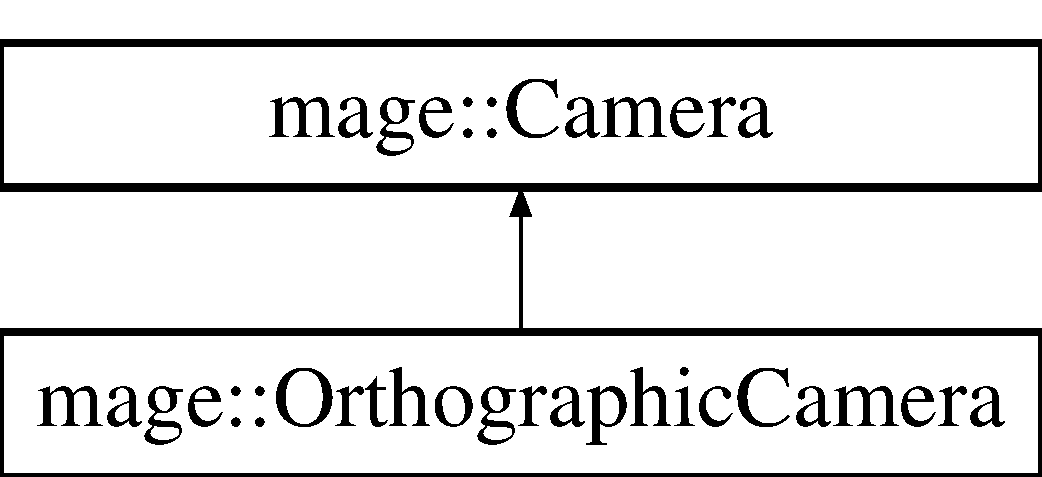
\includegraphics[height=2.000000cm]{classmage_1_1_orthographic_camera}
\end{center}
\end{figure}
\subsection*{Private Member Functions}
\begin{DoxyCompactItemize}
\item 
\hyperlink{classmage_1_1_orthographic_camera_a02855f1a1830b51d98cf7c6adb22bf11}{Orthographic\+Camera} (float width, float height, float near\+\_\+z=M\+A\+G\+E\+\_\+\+D\+E\+F\+A\+U\+L\+T\+\_\+\+C\+A\+M\+E\+R\+A\+\_\+\+N\+E\+A\+R\+\_\+Z, float far\+\_\+z=M\+A\+G\+E\+\_\+\+D\+E\+F\+A\+U\+L\+T\+\_\+\+C\+A\+M\+E\+R\+A\+\_\+\+F\+A\+R\+\_\+Z)
\item 
\hyperlink{classmage_1_1_orthographic_camera_aad12a2901577a187bb53e4c2e2f5a658}{Orthographic\+Camera} (const \hyperlink{classmage_1_1_orthographic_camera}{Orthographic\+Camera} \&camera)
\item 
virtual \hyperlink{classmage_1_1_orthographic_camera_a2ab3dbd44e2a6fad6a88e3733cc22ac9}{$\sim$\+Orthographic\+Camera} ()
\item 
\hyperlink{classmage_1_1_orthographic_camera}{Orthographic\+Camera} \& \hyperlink{classmage_1_1_orthographic_camera_a8ea679c9b4c3d2c6aef40119dbf60921}{operator=} (const \hyperlink{classmage_1_1_orthographic_camera}{Orthographic\+Camera} \&orthographic\+\_\+camera)
\item 
virtual \hyperlink{classmage_1_1_camera}{Camera} $\ast$ \hyperlink{classmage_1_1_orthographic_camera_a3fc2e5cfe7283670937de2a4841a5428}{Clone} () const
\item 
virtual X\+M\+M\+A\+T\+R\+IX \hyperlink{classmage_1_1_orthographic_camera_aedd86e56a0f7bc967ad8d9be2631a0cf}{Get\+View\+To\+Projection\+Matrix} () const override
\item 
void \hyperlink{classmage_1_1_orthographic_camera_a1ff2b3e4467049b978155d652a687c2d}{Set\+View\+To\+Projection\+Matrix} (float width, float height, float near\+\_\+z=M\+A\+G\+E\+\_\+\+D\+E\+F\+A\+U\+L\+T\+\_\+\+C\+A\+M\+E\+R\+A\+\_\+\+N\+E\+A\+R\+\_\+Z, float far\+\_\+z=M\+A\+G\+E\+\_\+\+D\+E\+F\+A\+U\+L\+T\+\_\+\+C\+A\+M\+E\+R\+A\+\_\+\+F\+A\+R\+\_\+Z)
\end{DoxyCompactItemize}
\subsection*{Additional Inherited Members}


\subsection{Detailed Description}
A class of orthographic cameras. 

\subsection{Constructor \& Destructor Documentation}
\hypertarget{classmage_1_1_orthographic_camera_a02855f1a1830b51d98cf7c6adb22bf11}{}\label{classmage_1_1_orthographic_camera_a02855f1a1830b51d98cf7c6adb22bf11} 
\index{mage\+::\+Orthographic\+Camera@{mage\+::\+Orthographic\+Camera}!Orthographic\+Camera@{Orthographic\+Camera}}
\index{Orthographic\+Camera@{Orthographic\+Camera}!mage\+::\+Orthographic\+Camera@{mage\+::\+Orthographic\+Camera}}
\subsubsection{\texorpdfstring{Orthographic\+Camera()}{OrthographicCamera()}\hspace{0.1cm}{\footnotesize\ttfamily [1/2]}}
{\footnotesize\ttfamily mage\+::\+Orthographic\+Camera\+::\+Orthographic\+Camera (\begin{DoxyParamCaption}\item[{float}]{width,  }\item[{float}]{height,  }\item[{float}]{near\+\_\+z = {\ttfamily MAGE\+\_\+DEFAULT\+\_\+CAMERA\+\_\+NEAR\+\_\+Z},  }\item[{float}]{far\+\_\+z = {\ttfamily MAGE\+\_\+DEFAULT\+\_\+CAMERA\+\_\+FAR\+\_\+Z} }\end{DoxyParamCaption})\hspace{0.3cm}{\ttfamily [private]}}

Constructs an orthographic camera.


\begin{DoxyParams}[1]{Parameters}
\mbox{\tt in}  & {\em width} & The width. \\
\hline
\mbox{\tt in}  & {\em height} & The height. \\
\hline
\mbox{\tt in}  & {\em near\+\_\+z} & The position of the near z-\/plane. \\
\hline
\mbox{\tt in}  & {\em far\+\_\+z} & The position of the far z-\/plane. \\
\hline
\end{DoxyParams}
\hypertarget{classmage_1_1_orthographic_camera_aad12a2901577a187bb53e4c2e2f5a658}{}\label{classmage_1_1_orthographic_camera_aad12a2901577a187bb53e4c2e2f5a658} 
\index{mage\+::\+Orthographic\+Camera@{mage\+::\+Orthographic\+Camera}!Orthographic\+Camera@{Orthographic\+Camera}}
\index{Orthographic\+Camera@{Orthographic\+Camera}!mage\+::\+Orthographic\+Camera@{mage\+::\+Orthographic\+Camera}}
\subsubsection{\texorpdfstring{Orthographic\+Camera()}{OrthographicCamera()}\hspace{0.1cm}{\footnotesize\ttfamily [2/2]}}
{\footnotesize\ttfamily mage\+::\+Orthographic\+Camera\+::\+Orthographic\+Camera (\begin{DoxyParamCaption}\item[{const \hyperlink{classmage_1_1_orthographic_camera}{Orthographic\+Camera} \&}]{camera }\end{DoxyParamCaption})\hspace{0.3cm}{\ttfamily [private]}}

Constructs an orthographic camera from the given orthographic camera.


\begin{DoxyParams}[1]{Parameters}
\mbox{\tt in}  & {\em camera} & A reference to the orthographic camera. \\
\hline
\end{DoxyParams}
\hypertarget{classmage_1_1_orthographic_camera_a2ab3dbd44e2a6fad6a88e3733cc22ac9}{}\label{classmage_1_1_orthographic_camera_a2ab3dbd44e2a6fad6a88e3733cc22ac9} 
\index{mage\+::\+Orthographic\+Camera@{mage\+::\+Orthographic\+Camera}!````~Orthographic\+Camera@{$\sim$\+Orthographic\+Camera}}
\index{````~Orthographic\+Camera@{$\sim$\+Orthographic\+Camera}!mage\+::\+Orthographic\+Camera@{mage\+::\+Orthographic\+Camera}}
\subsubsection{\texorpdfstring{$\sim$\+Orthographic\+Camera()}{~OrthographicCamera()}}
{\footnotesize\ttfamily virtual mage\+::\+Orthographic\+Camera\+::$\sim$\+Orthographic\+Camera (\begin{DoxyParamCaption}{ }\end{DoxyParamCaption})\hspace{0.3cm}{\ttfamily [private]}, {\ttfamily [virtual]}}

Destructs this orthographic camera. 

\subsection{Member Function Documentation}
\hypertarget{classmage_1_1_orthographic_camera_a3fc2e5cfe7283670937de2a4841a5428}{}\label{classmage_1_1_orthographic_camera_a3fc2e5cfe7283670937de2a4841a5428} 
\index{mage\+::\+Orthographic\+Camera@{mage\+::\+Orthographic\+Camera}!Clone@{Clone}}
\index{Clone@{Clone}!mage\+::\+Orthographic\+Camera@{mage\+::\+Orthographic\+Camera}}
\subsubsection{\texorpdfstring{Clone()}{Clone()}}
{\footnotesize\ttfamily virtual \hyperlink{classmage_1_1_camera}{Camera}$\ast$ mage\+::\+Orthographic\+Camera\+::\+Clone (\begin{DoxyParamCaption}{ }\end{DoxyParamCaption}) const\hspace{0.3cm}{\ttfamily [private]}, {\ttfamily [virtual]}}

Clones this orthographic camera.

\begin{DoxyReturn}{Returns}
A pointer to the clone of this orthographic camera. 
\end{DoxyReturn}


Implements \hyperlink{classmage_1_1_camera_a19301c2256c183db50b5e9406f7b5f3c}{mage\+::\+Camera}.

\hypertarget{classmage_1_1_orthographic_camera_aedd86e56a0f7bc967ad8d9be2631a0cf}{}\label{classmage_1_1_orthographic_camera_aedd86e56a0f7bc967ad8d9be2631a0cf} 
\index{mage\+::\+Orthographic\+Camera@{mage\+::\+Orthographic\+Camera}!Get\+View\+To\+Projection\+Matrix@{Get\+View\+To\+Projection\+Matrix}}
\index{Get\+View\+To\+Projection\+Matrix@{Get\+View\+To\+Projection\+Matrix}!mage\+::\+Orthographic\+Camera@{mage\+::\+Orthographic\+Camera}}
\subsubsection{\texorpdfstring{Get\+View\+To\+Projection\+Matrix()}{GetViewToProjectionMatrix()}}
{\footnotesize\ttfamily virtual X\+M\+M\+A\+T\+R\+IX mage\+::\+Orthographic\+Camera\+::\+Get\+View\+To\+Projection\+Matrix (\begin{DoxyParamCaption}{ }\end{DoxyParamCaption}) const\hspace{0.3cm}{\ttfamily [override]}, {\ttfamily [private]}, {\ttfamily [virtual]}}

Returns the view-\/to-\/projection matrix of this orthographic camera.

\begin{DoxyReturn}{Returns}
The view-\/to-\/projection matrix of this orthographic camera. 
\end{DoxyReturn}


Implements \hyperlink{classmage_1_1_camera_a1f5206864cf18b5548219492556df5d2}{mage\+::\+Camera}.

\hypertarget{classmage_1_1_orthographic_camera_a8ea679c9b4c3d2c6aef40119dbf60921}{}\label{classmage_1_1_orthographic_camera_a8ea679c9b4c3d2c6aef40119dbf60921} 
\index{mage\+::\+Orthographic\+Camera@{mage\+::\+Orthographic\+Camera}!operator=@{operator=}}
\index{operator=@{operator=}!mage\+::\+Orthographic\+Camera@{mage\+::\+Orthographic\+Camera}}
\subsubsection{\texorpdfstring{operator=()}{operator=()}}
{\footnotesize\ttfamily \hyperlink{classmage_1_1_orthographic_camera}{Orthographic\+Camera}\& mage\+::\+Orthographic\+Camera\+::operator= (\begin{DoxyParamCaption}\item[{const \hyperlink{classmage_1_1_orthographic_camera}{Orthographic\+Camera} \&}]{orthographic\+\_\+camera }\end{DoxyParamCaption})\hspace{0.3cm}{\ttfamily [private]}}

Copies the given orthographic camera to this orthographic camera.


\begin{DoxyParams}[1]{Parameters}
\mbox{\tt in}  & {\em orthographic\+\_\+camera} & The orthographic camera. \\
\hline
\end{DoxyParams}
\hypertarget{classmage_1_1_orthographic_camera_a1ff2b3e4467049b978155d652a687c2d}{}\label{classmage_1_1_orthographic_camera_a1ff2b3e4467049b978155d652a687c2d} 
\index{mage\+::\+Orthographic\+Camera@{mage\+::\+Orthographic\+Camera}!Set\+View\+To\+Projection\+Matrix@{Set\+View\+To\+Projection\+Matrix}}
\index{Set\+View\+To\+Projection\+Matrix@{Set\+View\+To\+Projection\+Matrix}!mage\+::\+Orthographic\+Camera@{mage\+::\+Orthographic\+Camera}}
\subsubsection{\texorpdfstring{Set\+View\+To\+Projection\+Matrix()}{SetViewToProjectionMatrix()}}
{\footnotesize\ttfamily void mage\+::\+Orthographic\+Camera\+::\+Set\+View\+To\+Projection\+Matrix (\begin{DoxyParamCaption}\item[{float}]{width,  }\item[{float}]{height,  }\item[{float}]{near\+\_\+z = {\ttfamily MAGE\+\_\+DEFAULT\+\_\+CAMERA\+\_\+NEAR\+\_\+Z},  }\item[{float}]{far\+\_\+z = {\ttfamily MAGE\+\_\+DEFAULT\+\_\+CAMERA\+\_\+FAR\+\_\+Z} }\end{DoxyParamCaption})\hspace{0.3cm}{\ttfamily [private]}}

Sets the view-\/to-\/projection matrix of this orthographic camera.


\begin{DoxyParams}[1]{Parameters}
\mbox{\tt in}  & {\em width} & The width. \\
\hline
\mbox{\tt in}  & {\em height} & The height. \\
\hline
\mbox{\tt in}  & {\em near\+\_\+z} & The position of the near z-\/plane. \\
\hline
\mbox{\tt in}  & {\em far\+\_\+z} & The position of the far z-\/plane. \\
\hline
\end{DoxyParams}

\hypertarget{classmage_1_1_parallel_for_loop}{}\section{mage\+:\+:Parallel\+For\+Loop Class Reference}
\label{classmage_1_1_parallel_for_loop}\index{mage\+::\+Parallel\+For\+Loop@{mage\+::\+Parallel\+For\+Loop}}
\subsection*{Public Member Functions}
\begin{DoxyCompactItemize}
\item 
\hyperlink{classmage_1_1_parallel_for_loop_aece78e3074ed1c04f49c62da400a1aa9}{Parallel\+For\+Loop} (function$<$ void(size\+\_\+t) $>$ \hyperlink{classmage_1_1_parallel_for_loop_a3651892e12fc6cdf87b7c74ffe68e82c}{func}, size\+\_\+t max\+\_\+index, size\+\_\+t chunk\+\_\+size)
\item 
bool \hyperlink{classmage_1_1_parallel_for_loop_a6ca9c77ef5475a0df0f742f2301d2d40}{Is\+Finished} () const
\end{DoxyCompactItemize}
\subsection*{Public Attributes}
\begin{DoxyCompactItemize}
\item 
function$<$ void(size\+\_\+t) $>$ \hyperlink{classmage_1_1_parallel_for_loop_a3651892e12fc6cdf87b7c74ffe68e82c}{func}
\item 
size\+\_\+t \hyperlink{classmage_1_1_parallel_for_loop_a3d0ef5cd968afc70d03cd1b740fcf4cb}{m\+\_\+next\+\_\+index}
\item 
const size\+\_\+t \hyperlink{classmage_1_1_parallel_for_loop_a1ef5e1094e5c20658a62faed566cb163}{m\+\_\+max\+\_\+index}
\item 
const size\+\_\+t \hyperlink{classmage_1_1_parallel_for_loop_a5c17c6e07dda15386c475dc2f80bd8ba}{m\+\_\+chunk\+\_\+size}
\item 
\hyperlink{classmage_1_1_parallel_for_loop}{Parallel\+For\+Loop} $\ast$ \hyperlink{classmage_1_1_parallel_for_loop_a8a0b3a82891160006795656c06c772da}{m\+\_\+next}
\item 
size\+\_\+t \hyperlink{classmage_1_1_parallel_for_loop_ae991b27616bf56e3660124e4d0b7d0ef}{m\+\_\+active\+\_\+workers}
\end{DoxyCompactItemize}


\subsection{Constructor \& Destructor Documentation}
\hypertarget{classmage_1_1_parallel_for_loop_aece78e3074ed1c04f49c62da400a1aa9}{}\label{classmage_1_1_parallel_for_loop_aece78e3074ed1c04f49c62da400a1aa9} 
\index{mage\+::\+Parallel\+For\+Loop@{mage\+::\+Parallel\+For\+Loop}!Parallel\+For\+Loop@{Parallel\+For\+Loop}}
\index{Parallel\+For\+Loop@{Parallel\+For\+Loop}!mage\+::\+Parallel\+For\+Loop@{mage\+::\+Parallel\+For\+Loop}}
\subsubsection{\texorpdfstring{Parallel\+For\+Loop()}{ParallelForLoop()}}
{\footnotesize\ttfamily mage\+::\+Parallel\+For\+Loop\+::\+Parallel\+For\+Loop (\begin{DoxyParamCaption}\item[{function$<$ void(size\+\_\+t) $>$}]{func,  }\item[{size\+\_\+t}]{max\+\_\+index,  }\item[{size\+\_\+t}]{chunk\+\_\+size }\end{DoxyParamCaption})}



\subsection{Member Function Documentation}
\hypertarget{classmage_1_1_parallel_for_loop_a6ca9c77ef5475a0df0f742f2301d2d40}{}\label{classmage_1_1_parallel_for_loop_a6ca9c77ef5475a0df0f742f2301d2d40} 
\index{mage\+::\+Parallel\+For\+Loop@{mage\+::\+Parallel\+For\+Loop}!Is\+Finished@{Is\+Finished}}
\index{Is\+Finished@{Is\+Finished}!mage\+::\+Parallel\+For\+Loop@{mage\+::\+Parallel\+For\+Loop}}
\subsubsection{\texorpdfstring{Is\+Finished()}{IsFinished()}}
{\footnotesize\ttfamily bool mage\+::\+Parallel\+For\+Loop\+::\+Is\+Finished (\begin{DoxyParamCaption}{ }\end{DoxyParamCaption}) const}



\subsection{Member Data Documentation}
\hypertarget{classmage_1_1_parallel_for_loop_a3651892e12fc6cdf87b7c74ffe68e82c}{}\label{classmage_1_1_parallel_for_loop_a3651892e12fc6cdf87b7c74ffe68e82c} 
\index{mage\+::\+Parallel\+For\+Loop@{mage\+::\+Parallel\+For\+Loop}!func@{func}}
\index{func@{func}!mage\+::\+Parallel\+For\+Loop@{mage\+::\+Parallel\+For\+Loop}}
\subsubsection{\texorpdfstring{func}{func}}
{\footnotesize\ttfamily function$<$ void(size\+\_\+t) $>$ mage\+::\+Parallel\+For\+Loop\+::func}

\hypertarget{classmage_1_1_parallel_for_loop_ae991b27616bf56e3660124e4d0b7d0ef}{}\label{classmage_1_1_parallel_for_loop_ae991b27616bf56e3660124e4d0b7d0ef} 
\index{mage\+::\+Parallel\+For\+Loop@{mage\+::\+Parallel\+For\+Loop}!m\+\_\+active\+\_\+workers@{m\+\_\+active\+\_\+workers}}
\index{m\+\_\+active\+\_\+workers@{m\+\_\+active\+\_\+workers}!mage\+::\+Parallel\+For\+Loop@{mage\+::\+Parallel\+For\+Loop}}
\subsubsection{\texorpdfstring{m\+\_\+active\+\_\+workers}{m\_active\_workers}}
{\footnotesize\ttfamily size\+\_\+t mage\+::\+Parallel\+For\+Loop\+::m\+\_\+active\+\_\+workers}

\hypertarget{classmage_1_1_parallel_for_loop_a5c17c6e07dda15386c475dc2f80bd8ba}{}\label{classmage_1_1_parallel_for_loop_a5c17c6e07dda15386c475dc2f80bd8ba} 
\index{mage\+::\+Parallel\+For\+Loop@{mage\+::\+Parallel\+For\+Loop}!m\+\_\+chunk\+\_\+size@{m\+\_\+chunk\+\_\+size}}
\index{m\+\_\+chunk\+\_\+size@{m\+\_\+chunk\+\_\+size}!mage\+::\+Parallel\+For\+Loop@{mage\+::\+Parallel\+For\+Loop}}
\subsubsection{\texorpdfstring{m\+\_\+chunk\+\_\+size}{m\_chunk\_size}}
{\footnotesize\ttfamily const size\+\_\+t mage\+::\+Parallel\+For\+Loop\+::m\+\_\+chunk\+\_\+size}

\hypertarget{classmage_1_1_parallel_for_loop_a1ef5e1094e5c20658a62faed566cb163}{}\label{classmage_1_1_parallel_for_loop_a1ef5e1094e5c20658a62faed566cb163} 
\index{mage\+::\+Parallel\+For\+Loop@{mage\+::\+Parallel\+For\+Loop}!m\+\_\+max\+\_\+index@{m\+\_\+max\+\_\+index}}
\index{m\+\_\+max\+\_\+index@{m\+\_\+max\+\_\+index}!mage\+::\+Parallel\+For\+Loop@{mage\+::\+Parallel\+For\+Loop}}
\subsubsection{\texorpdfstring{m\+\_\+max\+\_\+index}{m\_max\_index}}
{\footnotesize\ttfamily const size\+\_\+t mage\+::\+Parallel\+For\+Loop\+::m\+\_\+max\+\_\+index}

\hypertarget{classmage_1_1_parallel_for_loop_a8a0b3a82891160006795656c06c772da}{}\label{classmage_1_1_parallel_for_loop_a8a0b3a82891160006795656c06c772da} 
\index{mage\+::\+Parallel\+For\+Loop@{mage\+::\+Parallel\+For\+Loop}!m\+\_\+next@{m\+\_\+next}}
\index{m\+\_\+next@{m\+\_\+next}!mage\+::\+Parallel\+For\+Loop@{mage\+::\+Parallel\+For\+Loop}}
\subsubsection{\texorpdfstring{m\+\_\+next}{m\_next}}
{\footnotesize\ttfamily \hyperlink{classmage_1_1_parallel_for_loop}{Parallel\+For\+Loop}$\ast$ mage\+::\+Parallel\+For\+Loop\+::m\+\_\+next}

\hypertarget{classmage_1_1_parallel_for_loop_a3d0ef5cd968afc70d03cd1b740fcf4cb}{}\label{classmage_1_1_parallel_for_loop_a3d0ef5cd968afc70d03cd1b740fcf4cb} 
\index{mage\+::\+Parallel\+For\+Loop@{mage\+::\+Parallel\+For\+Loop}!m\+\_\+next\+\_\+index@{m\+\_\+next\+\_\+index}}
\index{m\+\_\+next\+\_\+index@{m\+\_\+next\+\_\+index}!mage\+::\+Parallel\+For\+Loop@{mage\+::\+Parallel\+For\+Loop}}
\subsubsection{\texorpdfstring{m\+\_\+next\+\_\+index}{m\_next\_index}}
{\footnotesize\ttfamily size\+\_\+t mage\+::\+Parallel\+For\+Loop\+::m\+\_\+next\+\_\+index}


\hypertarget{classmage_1_1_perspective_camera}{}\section{mage\+:\+:Perspective\+Camera Class Reference}
\label{classmage_1_1_perspective_camera}\index{mage\+::\+Perspective\+Camera@{mage\+::\+Perspective\+Camera}}


{\ttfamily \#include $<$perspective\+\_\+camera.\+hpp$>$}

Inheritance diagram for mage\+:\+:Perspective\+Camera\+:\begin{figure}[H]
\begin{center}
\leavevmode
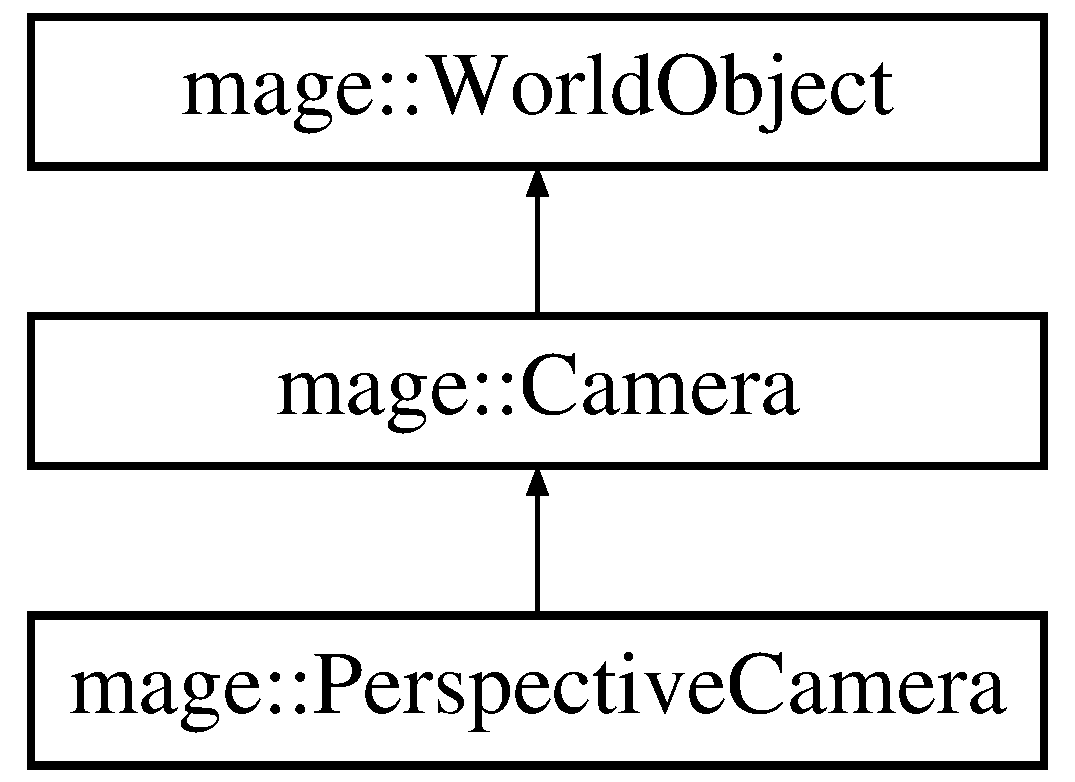
\includegraphics[height=2.000000cm]{classmage_1_1_perspective_camera}
\end{center}
\end{figure}
\subsection*{Public Member Functions}
\begin{DoxyCompactItemize}
\item 
\hyperlink{classmage_1_1_perspective_camera_aef3998fca25cb7d99b9a03ef9483040d}{Perspective\+Camera} (float width, float height, float fov\+\_\+y=M\+A\+G\+E\+\_\+\+D\+E\+F\+A\+U\+L\+T\+\_\+\+C\+A\+M\+E\+R\+A\+\_\+\+F\+O\+V\+\_\+Y, float near\+\_\+z=M\+A\+G\+E\+\_\+\+D\+E\+F\+A\+U\+L\+T\+\_\+\+C\+A\+M\+E\+R\+A\+\_\+\+N\+E\+A\+R\+\_\+Z, float far\+\_\+z=M\+A\+G\+E\+\_\+\+D\+E\+F\+A\+U\+L\+T\+\_\+\+C\+A\+M\+E\+R\+A\+\_\+\+F\+A\+R\+\_\+Z)
\item 
\hyperlink{classmage_1_1_perspective_camera_a198d1460d9312af27ed6ef2ac28b616d}{Perspective\+Camera} (const \hyperlink{classmage_1_1_perspective_camera}{Perspective\+Camera} \&camera)
\item 
virtual \hyperlink{classmage_1_1_perspective_camera_abf42546e2560d7d62e7e62680a6da02b}{$\sim$\+Perspective\+Camera} ()
\item 
\hyperlink{classmage_1_1_perspective_camera}{Perspective\+Camera} \& \hyperlink{classmage_1_1_perspective_camera_ac4c9ab3a10fac363e6779570c4905d65}{operator=} (const \hyperlink{classmage_1_1_perspective_camera}{Perspective\+Camera} \&perspective\+\_\+camera)
\item 
virtual \hyperlink{classmage_1_1_camera}{Camera} $\ast$ \hyperlink{classmage_1_1_perspective_camera_aa2fae7b2ca5daadeda0fd935fcdb101a}{Clone} () const
\item 
float \hyperlink{classmage_1_1_perspective_camera_a15223034b30ca691c51de8850c033293}{Get\+F\+O\+VY} () const
\item 
\hyperlink{classmage_1_1_camera}{Camera} \& \hyperlink{classmage_1_1_perspective_camera_a00033fc6b25206c40a056ce142fecfee}{Set\+F\+O\+VY} (float fov\+\_\+y)
\item 
float \hyperlink{classmage_1_1_perspective_camera_ab74cbd2777d5b430da5702a12b1b451e}{Get\+Aspect\+Ratio} () const
\item 
virtual X\+M\+M\+A\+T\+R\+IX \hyperlink{classmage_1_1_perspective_camera_a83a38a4e8180707df2323130f9cee4a5}{Get\+View\+To\+Projection\+Matrix} () const override
\item 
void \hyperlink{classmage_1_1_perspective_camera_adef65223ab45c65cebf712dd14cea942}{Set\+View\+To\+Projection\+Matrix} (float width, float height, float fov\+\_\+y=M\+A\+G\+E\+\_\+\+D\+E\+F\+A\+U\+L\+T\+\_\+\+C\+A\+M\+E\+R\+A\+\_\+\+F\+O\+V\+\_\+Y, float near\+\_\+z=M\+A\+G\+E\+\_\+\+D\+E\+F\+A\+U\+L\+T\+\_\+\+C\+A\+M\+E\+R\+A\+\_\+\+N\+E\+A\+R\+\_\+Z, float far\+\_\+z=M\+A\+G\+E\+\_\+\+D\+E\+F\+A\+U\+L\+T\+\_\+\+C\+A\+M\+E\+R\+A\+\_\+\+F\+A\+R\+\_\+Z)
\end{DoxyCompactItemize}
\subsection*{Private Attributes}
\begin{DoxyCompactItemize}
\item 
float \hyperlink{classmage_1_1_perspective_camera_abdcf1a0cdd247e0f7e14e70898678af6}{m\+\_\+fov\+\_\+y}
\end{DoxyCompactItemize}
\subsection*{Additional Inherited Members}


\subsection{Detailed Description}
A class of perspective camera. 

\subsection{Constructor \& Destructor Documentation}
\hypertarget{classmage_1_1_perspective_camera_aef3998fca25cb7d99b9a03ef9483040d}{}\label{classmage_1_1_perspective_camera_aef3998fca25cb7d99b9a03ef9483040d} 
\index{mage\+::\+Perspective\+Camera@{mage\+::\+Perspective\+Camera}!Perspective\+Camera@{Perspective\+Camera}}
\index{Perspective\+Camera@{Perspective\+Camera}!mage\+::\+Perspective\+Camera@{mage\+::\+Perspective\+Camera}}
\subsubsection{\texorpdfstring{Perspective\+Camera()}{PerspectiveCamera()}\hspace{0.1cm}{\footnotesize\ttfamily [1/2]}}
{\footnotesize\ttfamily mage\+::\+Perspective\+Camera\+::\+Perspective\+Camera (\begin{DoxyParamCaption}\item[{float}]{width,  }\item[{float}]{height,  }\item[{float}]{fov\+\_\+y = {\ttfamily MAGE\+\_\+DEFAULT\+\_\+CAMERA\+\_\+FOV\+\_\+Y},  }\item[{float}]{near\+\_\+z = {\ttfamily MAGE\+\_\+DEFAULT\+\_\+CAMERA\+\_\+NEAR\+\_\+Z},  }\item[{float}]{far\+\_\+z = {\ttfamily MAGE\+\_\+DEFAULT\+\_\+CAMERA\+\_\+FAR\+\_\+Z} }\end{DoxyParamCaption})}

Constructs a perspective camera.


\begin{DoxyParams}[1]{Parameters}
\mbox{\tt in}  & {\em width} & The width. \\
\hline
\mbox{\tt in}  & {\em height} & The height. \\
\hline
\mbox{\tt in}  & {\em fov\+\_\+y} & The vertical field-\/of-\/view. \\
\hline
\mbox{\tt in}  & {\em near\+\_\+z} & The position of the near z-\/plane. \\
\hline
\mbox{\tt in}  & {\em far\+\_\+z} & The position of the far z-\/plane. \\
\hline
\end{DoxyParams}
\hypertarget{classmage_1_1_perspective_camera_a198d1460d9312af27ed6ef2ac28b616d}{}\label{classmage_1_1_perspective_camera_a198d1460d9312af27ed6ef2ac28b616d} 
\index{mage\+::\+Perspective\+Camera@{mage\+::\+Perspective\+Camera}!Perspective\+Camera@{Perspective\+Camera}}
\index{Perspective\+Camera@{Perspective\+Camera}!mage\+::\+Perspective\+Camera@{mage\+::\+Perspective\+Camera}}
\subsubsection{\texorpdfstring{Perspective\+Camera()}{PerspectiveCamera()}\hspace{0.1cm}{\footnotesize\ttfamily [2/2]}}
{\footnotesize\ttfamily mage\+::\+Perspective\+Camera\+::\+Perspective\+Camera (\begin{DoxyParamCaption}\item[{const \hyperlink{classmage_1_1_perspective_camera}{Perspective\+Camera} \&}]{camera }\end{DoxyParamCaption})}

Constructs a perspective camera from the given perpsective camera.


\begin{DoxyParams}[1]{Parameters}
\mbox{\tt in}  & {\em camera} & A reference to the perspective camera. \\
\hline
\end{DoxyParams}
\hypertarget{classmage_1_1_perspective_camera_abf42546e2560d7d62e7e62680a6da02b}{}\label{classmage_1_1_perspective_camera_abf42546e2560d7d62e7e62680a6da02b} 
\index{mage\+::\+Perspective\+Camera@{mage\+::\+Perspective\+Camera}!````~Perspective\+Camera@{$\sim$\+Perspective\+Camera}}
\index{````~Perspective\+Camera@{$\sim$\+Perspective\+Camera}!mage\+::\+Perspective\+Camera@{mage\+::\+Perspective\+Camera}}
\subsubsection{\texorpdfstring{$\sim$\+Perspective\+Camera()}{~PerspectiveCamera()}}
{\footnotesize\ttfamily virtual mage\+::\+Perspective\+Camera\+::$\sim$\+Perspective\+Camera (\begin{DoxyParamCaption}{ }\end{DoxyParamCaption})\hspace{0.3cm}{\ttfamily [virtual]}}

Destructs this perspective camera. 

\subsection{Member Function Documentation}
\hypertarget{classmage_1_1_perspective_camera_aa2fae7b2ca5daadeda0fd935fcdb101a}{}\label{classmage_1_1_perspective_camera_aa2fae7b2ca5daadeda0fd935fcdb101a} 
\index{mage\+::\+Perspective\+Camera@{mage\+::\+Perspective\+Camera}!Clone@{Clone}}
\index{Clone@{Clone}!mage\+::\+Perspective\+Camera@{mage\+::\+Perspective\+Camera}}
\subsubsection{\texorpdfstring{Clone()}{Clone()}}
{\footnotesize\ttfamily virtual \hyperlink{classmage_1_1_camera}{Camera}$\ast$ mage\+::\+Perspective\+Camera\+::\+Clone (\begin{DoxyParamCaption}{ }\end{DoxyParamCaption}) const\hspace{0.3cm}{\ttfamily [virtual]}}

Clones this perspective camera.

\begin{DoxyReturn}{Returns}
A pointer to the clone of this perspective camera. 
\end{DoxyReturn}


Implements \hyperlink{classmage_1_1_camera_a19301c2256c183db50b5e9406f7b5f3c}{mage\+::\+Camera}.

\hypertarget{classmage_1_1_perspective_camera_ab74cbd2777d5b430da5702a12b1b451e}{}\label{classmage_1_1_perspective_camera_ab74cbd2777d5b430da5702a12b1b451e} 
\index{mage\+::\+Perspective\+Camera@{mage\+::\+Perspective\+Camera}!Get\+Aspect\+Ratio@{Get\+Aspect\+Ratio}}
\index{Get\+Aspect\+Ratio@{Get\+Aspect\+Ratio}!mage\+::\+Perspective\+Camera@{mage\+::\+Perspective\+Camera}}
\subsubsection{\texorpdfstring{Get\+Aspect\+Ratio()}{GetAspectRatio()}}
{\footnotesize\ttfamily float mage\+::\+Perspective\+Camera\+::\+Get\+Aspect\+Ratio (\begin{DoxyParamCaption}{ }\end{DoxyParamCaption}) const}

Returns the aspect ratio of this perspective camera.

\begin{DoxyReturn}{Returns}
The aspect ratio of this perspective camera. 
\end{DoxyReturn}
\hypertarget{classmage_1_1_perspective_camera_a15223034b30ca691c51de8850c033293}{}\label{classmage_1_1_perspective_camera_a15223034b30ca691c51de8850c033293} 
\index{mage\+::\+Perspective\+Camera@{mage\+::\+Perspective\+Camera}!Get\+F\+O\+VY@{Get\+F\+O\+VY}}
\index{Get\+F\+O\+VY@{Get\+F\+O\+VY}!mage\+::\+Perspective\+Camera@{mage\+::\+Perspective\+Camera}}
\subsubsection{\texorpdfstring{Get\+F\+O\+V\+Y()}{GetFOVY()}}
{\footnotesize\ttfamily float mage\+::\+Perspective\+Camera\+::\+Get\+F\+O\+VY (\begin{DoxyParamCaption}{ }\end{DoxyParamCaption}) const}

Returns the vertical field-\/of-\/view of this perspective camera.

\begin{DoxyReturn}{Returns}
The vertical field-\/of-\/view of this perspective camera. 
\end{DoxyReturn}
\hypertarget{classmage_1_1_perspective_camera_a83a38a4e8180707df2323130f9cee4a5}{}\label{classmage_1_1_perspective_camera_a83a38a4e8180707df2323130f9cee4a5} 
\index{mage\+::\+Perspective\+Camera@{mage\+::\+Perspective\+Camera}!Get\+View\+To\+Projection\+Matrix@{Get\+View\+To\+Projection\+Matrix}}
\index{Get\+View\+To\+Projection\+Matrix@{Get\+View\+To\+Projection\+Matrix}!mage\+::\+Perspective\+Camera@{mage\+::\+Perspective\+Camera}}
\subsubsection{\texorpdfstring{Get\+View\+To\+Projection\+Matrix()}{GetViewToProjectionMatrix()}}
{\footnotesize\ttfamily virtual X\+M\+M\+A\+T\+R\+IX mage\+::\+Perspective\+Camera\+::\+Get\+View\+To\+Projection\+Matrix (\begin{DoxyParamCaption}{ }\end{DoxyParamCaption}) const\hspace{0.3cm}{\ttfamily [override]}, {\ttfamily [virtual]}}

Returns the view-\/to-\/projection matrix of this perspective camera.

\begin{DoxyReturn}{Returns}
The view-\/to-\/projection matrix of this perspective camera. 
\end{DoxyReturn}


Implements \hyperlink{classmage_1_1_camera_a1f5206864cf18b5548219492556df5d2}{mage\+::\+Camera}.

\hypertarget{classmage_1_1_perspective_camera_ac4c9ab3a10fac363e6779570c4905d65}{}\label{classmage_1_1_perspective_camera_ac4c9ab3a10fac363e6779570c4905d65} 
\index{mage\+::\+Perspective\+Camera@{mage\+::\+Perspective\+Camera}!operator=@{operator=}}
\index{operator=@{operator=}!mage\+::\+Perspective\+Camera@{mage\+::\+Perspective\+Camera}}
\subsubsection{\texorpdfstring{operator=()}{operator=()}}
{\footnotesize\ttfamily \hyperlink{classmage_1_1_perspective_camera}{Perspective\+Camera}\& mage\+::\+Perspective\+Camera\+::operator= (\begin{DoxyParamCaption}\item[{const \hyperlink{classmage_1_1_perspective_camera}{Perspective\+Camera} \&}]{perspective\+\_\+camera }\end{DoxyParamCaption})}

Copies the given perspective camera to this perspective camera.


\begin{DoxyParams}[1]{Parameters}
\mbox{\tt in}  & {\em perspective\+\_\+camera} & The perspective camera. \\
\hline
\end{DoxyParams}
\hypertarget{classmage_1_1_perspective_camera_a00033fc6b25206c40a056ce142fecfee}{}\label{classmage_1_1_perspective_camera_a00033fc6b25206c40a056ce142fecfee} 
\index{mage\+::\+Perspective\+Camera@{mage\+::\+Perspective\+Camera}!Set\+F\+O\+VY@{Set\+F\+O\+VY}}
\index{Set\+F\+O\+VY@{Set\+F\+O\+VY}!mage\+::\+Perspective\+Camera@{mage\+::\+Perspective\+Camera}}
\subsubsection{\texorpdfstring{Set\+F\+O\+V\+Y()}{SetFOVY()}}
{\footnotesize\ttfamily \hyperlink{classmage_1_1_camera}{Camera}\& mage\+::\+Perspective\+Camera\+::\+Set\+F\+O\+VY (\begin{DoxyParamCaption}\item[{float}]{fov\+\_\+y }\end{DoxyParamCaption})}

Sets the vertical field-\/of-\/view of this perspective camera to the given value.


\begin{DoxyParams}[1]{Parameters}
\mbox{\tt in}  & {\em fov\+\_\+y} & The vertical field-\/of-\/view. \\
\hline
\end{DoxyParams}
\begin{DoxyReturn}{Returns}
A reference to this perspective camera. 
\end{DoxyReturn}
\hypertarget{classmage_1_1_perspective_camera_adef65223ab45c65cebf712dd14cea942}{}\label{classmage_1_1_perspective_camera_adef65223ab45c65cebf712dd14cea942} 
\index{mage\+::\+Perspective\+Camera@{mage\+::\+Perspective\+Camera}!Set\+View\+To\+Projection\+Matrix@{Set\+View\+To\+Projection\+Matrix}}
\index{Set\+View\+To\+Projection\+Matrix@{Set\+View\+To\+Projection\+Matrix}!mage\+::\+Perspective\+Camera@{mage\+::\+Perspective\+Camera}}
\subsubsection{\texorpdfstring{Set\+View\+To\+Projection\+Matrix()}{SetViewToProjectionMatrix()}}
{\footnotesize\ttfamily void mage\+::\+Perspective\+Camera\+::\+Set\+View\+To\+Projection\+Matrix (\begin{DoxyParamCaption}\item[{float}]{width,  }\item[{float}]{height,  }\item[{float}]{fov\+\_\+y = {\ttfamily MAGE\+\_\+DEFAULT\+\_\+CAMERA\+\_\+FOV\+\_\+Y},  }\item[{float}]{near\+\_\+z = {\ttfamily MAGE\+\_\+DEFAULT\+\_\+CAMERA\+\_\+NEAR\+\_\+Z},  }\item[{float}]{far\+\_\+z = {\ttfamily MAGE\+\_\+DEFAULT\+\_\+CAMERA\+\_\+FAR\+\_\+Z} }\end{DoxyParamCaption})}

Sets the view-\/to-\/projection matrix of this perspective camera.


\begin{DoxyParams}[1]{Parameters}
\mbox{\tt in}  & {\em width} & The width. \\
\hline
\mbox{\tt in}  & {\em height} & The height. \\
\hline
\mbox{\tt in}  & {\em fov\+\_\+y} & The vertical field-\/of-\/view. \\
\hline
\mbox{\tt in}  & {\em near\+\_\+z} & The position of the near z-\/plane. \\
\hline
\mbox{\tt in}  & {\em far\+\_\+z} & The position of the far z-\/plane. \\
\hline
\end{DoxyParams}


\subsection{Member Data Documentation}
\hypertarget{classmage_1_1_perspective_camera_abdcf1a0cdd247e0f7e14e70898678af6}{}\label{classmage_1_1_perspective_camera_abdcf1a0cdd247e0f7e14e70898678af6} 
\index{mage\+::\+Perspective\+Camera@{mage\+::\+Perspective\+Camera}!m\+\_\+fov\+\_\+y@{m\+\_\+fov\+\_\+y}}
\index{m\+\_\+fov\+\_\+y@{m\+\_\+fov\+\_\+y}!mage\+::\+Perspective\+Camera@{mage\+::\+Perspective\+Camera}}
\subsubsection{\texorpdfstring{m\+\_\+fov\+\_\+y}{m\_fov\_y}}
{\footnotesize\ttfamily float mage\+::\+Perspective\+Camera\+::m\+\_\+fov\+\_\+y\hspace{0.3cm}{\ttfamily [private]}}

The vertical field-\/of-\/view of this perspective camera. 
\hypertarget{classmage_1_1_progress_reporter}{}\section{mage\+:\+:Progress\+Reporter Class Reference}
\label{classmage_1_1_progress_reporter}\index{mage\+::\+Progress\+Reporter@{mage\+::\+Progress\+Reporter}}


{\ttfamily \#include $<$progress\+\_\+reporter.\+hpp$>$}

\subsection*{Public Member Functions}
\begin{DoxyCompactItemize}
\item 
\hyperlink{classmage_1_1_progress_reporter_ab105fa7ac8fb1c53c60deab107c26f74}{Progress\+Reporter} (const string \&title, uint32\+\_\+t nb\+\_\+work, char plus\+\_\+char=\textquotesingle{}+\textquotesingle{}, uint32\+\_\+t bar\+\_\+length=0)
\item 
virtual \hyperlink{classmage_1_1_progress_reporter_aa543239c6dd4474a77cf4cf6904c1b26}{$\sim$\+Progress\+Reporter} ()
\item 
void \hyperlink{classmage_1_1_progress_reporter_a0a5f99f15e4152da9a3d6aadd888244a}{Update} (uint32\+\_\+t nb\+\_\+work=1)
\item 
void \hyperlink{classmage_1_1_progress_reporter_a11d758647ac2082bc296ab53a7454eaa}{Done} ()
\end{DoxyCompactItemize}
\subsection*{Protected Attributes}
\begin{DoxyCompactItemize}
\item 
const uint32\+\_\+t \hyperlink{classmage_1_1_progress_reporter_a1b0c8d8f3cde82161b34897c5e95e09b}{m\+\_\+nb\+\_\+work\+\_\+total}
\item 
uint32\+\_\+t \hyperlink{classmage_1_1_progress_reporter_ad3cb941594f138c208fa522a355a985b}{m\+\_\+nb\+\_\+work\+\_\+done}
\item 
uint32\+\_\+t \hyperlink{classmage_1_1_progress_reporter_aeae54fa7c542ccfbdaa44c0942c483fd}{m\+\_\+nb\+\_\+plusses\+\_\+total}
\item 
uint32\+\_\+t \hyperlink{classmage_1_1_progress_reporter_a17d7a4f8b2c8a6de255786f6165726bd}{m\+\_\+nb\+\_\+plusses\+\_\+printed}
\item 
\hyperlink{namespacemage_a8c307fbcc33bce9b7f2aa4c26c3b95cf}{Unique\+Ptr}$<$ \hyperlink{classmage_1_1_timer}{Timer} $>$ \hyperlink{classmage_1_1_progress_reporter_a4c5c81ce84ceaab7764bd640a18db788}{m\+\_\+timer}
\item 
F\+I\+LE $\ast$ \hyperlink{classmage_1_1_progress_reporter_ad325ee5978fd1d16a97acbe37a977982}{m\+\_\+fout}
\item 
const char \hyperlink{classmage_1_1_progress_reporter_ab3c8d12e79e63ae2b99fde8d6627c230}{m\+\_\+plus\+\_\+char}
\item 
char $\ast$ \hyperlink{classmage_1_1_progress_reporter_a3aa49d5b886263402d9a9ecb4851670c}{m\+\_\+buffer}
\item 
char $\ast$ \hyperlink{classmage_1_1_progress_reporter_a7adafaaf90edf29c8c27f4008aea41c9}{m\+\_\+current\+\_\+pos}
\item 
\hyperlink{classmage_1_1_mutex}{Mutex} $\ast$ \hyperlink{classmage_1_1_progress_reporter_abda37942e51b682b2871e49883d58da1}{m\+\_\+mutex}
\end{DoxyCompactItemize}
\subsection*{Private Member Functions}
\begin{DoxyCompactItemize}
\item 
\hyperlink{classmage_1_1_progress_reporter_a59c1ca6e4c0d480a1726d79ef6d42e74}{Progress\+Reporter} (const \hyperlink{classmage_1_1_progress_reporter}{Progress\+Reporter} \&progress\+\_\+reporter)=delete
\item 
\hyperlink{classmage_1_1_progress_reporter}{Progress\+Reporter} \& \hyperlink{classmage_1_1_progress_reporter_a7bc52147f6d2e30d897f512f910c8917}{operator=} (const \hyperlink{classmage_1_1_progress_reporter}{Progress\+Reporter} \&progress\+\_\+reporter)=delete
\end{DoxyCompactItemize}


\subsection{Detailed Description}
A class of progress reporters. 

\subsection{Constructor \& Destructor Documentation}
\hypertarget{classmage_1_1_progress_reporter_ab105fa7ac8fb1c53c60deab107c26f74}{}\label{classmage_1_1_progress_reporter_ab105fa7ac8fb1c53c60deab107c26f74} 
\index{mage\+::\+Progress\+Reporter@{mage\+::\+Progress\+Reporter}!Progress\+Reporter@{Progress\+Reporter}}
\index{Progress\+Reporter@{Progress\+Reporter}!mage\+::\+Progress\+Reporter@{mage\+::\+Progress\+Reporter}}
\subsubsection{\texorpdfstring{Progress\+Reporter()}{ProgressReporter()}\hspace{0.1cm}{\footnotesize\ttfamily [1/2]}}
{\footnotesize\ttfamily mage\+::\+Progress\+Reporter\+::\+Progress\+Reporter (\begin{DoxyParamCaption}\item[{const string \&}]{title,  }\item[{uint32\+\_\+t}]{nb\+\_\+work,  }\item[{char}]{plus\+\_\+char = {\ttfamily \textquotesingle{}+\textquotesingle{}},  }\item[{uint32\+\_\+t}]{bar\+\_\+length = {\ttfamily 0} }\end{DoxyParamCaption})}

Constructs a progress reporter.


\begin{DoxyParams}[1]{Parameters}
\mbox{\tt in}  & {\em title} & A reference to the title. \\
\hline
\mbox{\tt in}  & {\em nb\+\_\+work} & The total number of work units. \\
\hline
\mbox{\tt in}  & {\em plus\+\_\+char} & The character representing a work unit that is already done. \\
\hline
\mbox{\tt in}  & {\em bar\+\_\+length} & The length of the progress bar. If 0 the default length will be chosen. \\
\hline
\end{DoxyParams}
\hypertarget{classmage_1_1_progress_reporter_aa543239c6dd4474a77cf4cf6904c1b26}{}\label{classmage_1_1_progress_reporter_aa543239c6dd4474a77cf4cf6904c1b26} 
\index{mage\+::\+Progress\+Reporter@{mage\+::\+Progress\+Reporter}!````~Progress\+Reporter@{$\sim$\+Progress\+Reporter}}
\index{````~Progress\+Reporter@{$\sim$\+Progress\+Reporter}!mage\+::\+Progress\+Reporter@{mage\+::\+Progress\+Reporter}}
\subsubsection{\texorpdfstring{$\sim$\+Progress\+Reporter()}{~ProgressReporter()}}
{\footnotesize\ttfamily mage\+::\+Progress\+Reporter\+::$\sim$\+Progress\+Reporter (\begin{DoxyParamCaption}{ }\end{DoxyParamCaption})\hspace{0.3cm}{\ttfamily [virtual]}}

Destructs this progress reporter. \hypertarget{classmage_1_1_progress_reporter_a59c1ca6e4c0d480a1726d79ef6d42e74}{}\label{classmage_1_1_progress_reporter_a59c1ca6e4c0d480a1726d79ef6d42e74} 
\index{mage\+::\+Progress\+Reporter@{mage\+::\+Progress\+Reporter}!Progress\+Reporter@{Progress\+Reporter}}
\index{Progress\+Reporter@{Progress\+Reporter}!mage\+::\+Progress\+Reporter@{mage\+::\+Progress\+Reporter}}
\subsubsection{\texorpdfstring{Progress\+Reporter()}{ProgressReporter()}\hspace{0.1cm}{\footnotesize\ttfamily [2/2]}}
{\footnotesize\ttfamily mage\+::\+Progress\+Reporter\+::\+Progress\+Reporter (\begin{DoxyParamCaption}\item[{const \hyperlink{classmage_1_1_progress_reporter}{Progress\+Reporter} \&}]{progress\+\_\+reporter }\end{DoxyParamCaption})\hspace{0.3cm}{\ttfamily [private]}, {\ttfamily [delete]}}

Constructs a progress reporter from the given progress reporter.


\begin{DoxyParams}[1]{Parameters}
\mbox{\tt in}  & {\em progress\+\_\+reporter} & A reference to the progress reporter. \\
\hline
\end{DoxyParams}


\subsection{Member Function Documentation}
\hypertarget{classmage_1_1_progress_reporter_a11d758647ac2082bc296ab53a7454eaa}{}\label{classmage_1_1_progress_reporter_a11d758647ac2082bc296ab53a7454eaa} 
\index{mage\+::\+Progress\+Reporter@{mage\+::\+Progress\+Reporter}!Done@{Done}}
\index{Done@{Done}!mage\+::\+Progress\+Reporter@{mage\+::\+Progress\+Reporter}}
\subsubsection{\texorpdfstring{Done()}{Done()}}
{\footnotesize\ttfamily void mage\+::\+Progress\+Reporter\+::\+Done (\begin{DoxyParamCaption}{ }\end{DoxyParamCaption})}

Finishes this progress reporter. \hypertarget{classmage_1_1_progress_reporter_a7bc52147f6d2e30d897f512f910c8917}{}\label{classmage_1_1_progress_reporter_a7bc52147f6d2e30d897f512f910c8917} 
\index{mage\+::\+Progress\+Reporter@{mage\+::\+Progress\+Reporter}!operator=@{operator=}}
\index{operator=@{operator=}!mage\+::\+Progress\+Reporter@{mage\+::\+Progress\+Reporter}}
\subsubsection{\texorpdfstring{operator=()}{operator=()}}
{\footnotesize\ttfamily \hyperlink{classmage_1_1_progress_reporter}{Progress\+Reporter}\& mage\+::\+Progress\+Reporter\+::operator= (\begin{DoxyParamCaption}\item[{const \hyperlink{classmage_1_1_progress_reporter}{Progress\+Reporter} \&}]{progress\+\_\+reporter }\end{DoxyParamCaption})\hspace{0.3cm}{\ttfamily [private]}, {\ttfamily [delete]}}

Copies the given progress reporter to this progress reporter.


\begin{DoxyParams}[1]{Parameters}
\mbox{\tt in}  & {\em progress\+\_\+reporter} & A reference to the progress reporter to copy from. \\
\hline
\end{DoxyParams}
\begin{DoxyReturn}{Returns}
A reference to the copy of the given progress reporter (i.\+e. this progress reporter). 
\end{DoxyReturn}
\hypertarget{classmage_1_1_progress_reporter_a0a5f99f15e4152da9a3d6aadd888244a}{}\label{classmage_1_1_progress_reporter_a0a5f99f15e4152da9a3d6aadd888244a} 
\index{mage\+::\+Progress\+Reporter@{mage\+::\+Progress\+Reporter}!Update@{Update}}
\index{Update@{Update}!mage\+::\+Progress\+Reporter@{mage\+::\+Progress\+Reporter}}
\subsubsection{\texorpdfstring{Update()}{Update()}}
{\footnotesize\ttfamily void mage\+::\+Progress\+Reporter\+::\+Update (\begin{DoxyParamCaption}\item[{uint32\+\_\+t}]{nb\+\_\+work = {\ttfamily 1} }\end{DoxyParamCaption})}

Updates this progress reporter.


\begin{DoxyParams}[1]{Parameters}
\mbox{\tt in}  & {\em nb\+\_\+work} & The number of work units that are done. \\
\hline
\end{DoxyParams}


\subsection{Member Data Documentation}
\hypertarget{classmage_1_1_progress_reporter_a3aa49d5b886263402d9a9ecb4851670c}{}\label{classmage_1_1_progress_reporter_a3aa49d5b886263402d9a9ecb4851670c} 
\index{mage\+::\+Progress\+Reporter@{mage\+::\+Progress\+Reporter}!m\+\_\+buffer@{m\+\_\+buffer}}
\index{m\+\_\+buffer@{m\+\_\+buffer}!mage\+::\+Progress\+Reporter@{mage\+::\+Progress\+Reporter}}
\subsubsection{\texorpdfstring{m\+\_\+buffer}{m\_buffer}}
{\footnotesize\ttfamily char$\ast$ mage\+::\+Progress\+Reporter\+::m\+\_\+buffer\hspace{0.3cm}{\ttfamily [protected]}}

The output buffer of this progress reporter. \hypertarget{classmage_1_1_progress_reporter_a7adafaaf90edf29c8c27f4008aea41c9}{}\label{classmage_1_1_progress_reporter_a7adafaaf90edf29c8c27f4008aea41c9} 
\index{mage\+::\+Progress\+Reporter@{mage\+::\+Progress\+Reporter}!m\+\_\+current\+\_\+pos@{m\+\_\+current\+\_\+pos}}
\index{m\+\_\+current\+\_\+pos@{m\+\_\+current\+\_\+pos}!mage\+::\+Progress\+Reporter@{mage\+::\+Progress\+Reporter}}
\subsubsection{\texorpdfstring{m\+\_\+current\+\_\+pos}{m\_current\_pos}}
{\footnotesize\ttfamily char$\ast$ mage\+::\+Progress\+Reporter\+::m\+\_\+current\+\_\+pos\hspace{0.3cm}{\ttfamily [protected]}}

The current (output) position of this progress reporter. \hypertarget{classmage_1_1_progress_reporter_ad325ee5978fd1d16a97acbe37a977982}{}\label{classmage_1_1_progress_reporter_ad325ee5978fd1d16a97acbe37a977982} 
\index{mage\+::\+Progress\+Reporter@{mage\+::\+Progress\+Reporter}!m\+\_\+fout@{m\+\_\+fout}}
\index{m\+\_\+fout@{m\+\_\+fout}!mage\+::\+Progress\+Reporter@{mage\+::\+Progress\+Reporter}}
\subsubsection{\texorpdfstring{m\+\_\+fout}{m\_fout}}
{\footnotesize\ttfamily F\+I\+LE$\ast$ mage\+::\+Progress\+Reporter\+::m\+\_\+fout\hspace{0.3cm}{\ttfamily [protected]}}

The output file stream of this progress reporter. \hypertarget{classmage_1_1_progress_reporter_abda37942e51b682b2871e49883d58da1}{}\label{classmage_1_1_progress_reporter_abda37942e51b682b2871e49883d58da1} 
\index{mage\+::\+Progress\+Reporter@{mage\+::\+Progress\+Reporter}!m\+\_\+mutex@{m\+\_\+mutex}}
\index{m\+\_\+mutex@{m\+\_\+mutex}!mage\+::\+Progress\+Reporter@{mage\+::\+Progress\+Reporter}}
\subsubsection{\texorpdfstring{m\+\_\+mutex}{m\_mutex}}
{\footnotesize\ttfamily \hyperlink{classmage_1_1_mutex}{Mutex}$\ast$ mage\+::\+Progress\+Reporter\+::m\+\_\+mutex\hspace{0.3cm}{\ttfamily [protected]}}

The mutex needed for updating this progress reporter. \hypertarget{classmage_1_1_progress_reporter_a17d7a4f8b2c8a6de255786f6165726bd}{}\label{classmage_1_1_progress_reporter_a17d7a4f8b2c8a6de255786f6165726bd} 
\index{mage\+::\+Progress\+Reporter@{mage\+::\+Progress\+Reporter}!m\+\_\+nb\+\_\+plusses\+\_\+printed@{m\+\_\+nb\+\_\+plusses\+\_\+printed}}
\index{m\+\_\+nb\+\_\+plusses\+\_\+printed@{m\+\_\+nb\+\_\+plusses\+\_\+printed}!mage\+::\+Progress\+Reporter@{mage\+::\+Progress\+Reporter}}
\subsubsection{\texorpdfstring{m\+\_\+nb\+\_\+plusses\+\_\+printed}{m\_nb\_plusses\_printed}}
{\footnotesize\ttfamily uint32\+\_\+t mage\+::\+Progress\+Reporter\+::m\+\_\+nb\+\_\+plusses\+\_\+printed\hspace{0.3cm}{\ttfamily [protected]}}

The total number of plusses that are already outputted. \hypertarget{classmage_1_1_progress_reporter_aeae54fa7c542ccfbdaa44c0942c483fd}{}\label{classmage_1_1_progress_reporter_aeae54fa7c542ccfbdaa44c0942c483fd} 
\index{mage\+::\+Progress\+Reporter@{mage\+::\+Progress\+Reporter}!m\+\_\+nb\+\_\+plusses\+\_\+total@{m\+\_\+nb\+\_\+plusses\+\_\+total}}
\index{m\+\_\+nb\+\_\+plusses\+\_\+total@{m\+\_\+nb\+\_\+plusses\+\_\+total}!mage\+::\+Progress\+Reporter@{mage\+::\+Progress\+Reporter}}
\subsubsection{\texorpdfstring{m\+\_\+nb\+\_\+plusses\+\_\+total}{m\_nb\_plusses\_total}}
{\footnotesize\ttfamily uint32\+\_\+t mage\+::\+Progress\+Reporter\+::m\+\_\+nb\+\_\+plusses\+\_\+total\hspace{0.3cm}{\ttfamily [protected]}}

The total number of plusses that need to be outputted. \hypertarget{classmage_1_1_progress_reporter_ad3cb941594f138c208fa522a355a985b}{}\label{classmage_1_1_progress_reporter_ad3cb941594f138c208fa522a355a985b} 
\index{mage\+::\+Progress\+Reporter@{mage\+::\+Progress\+Reporter}!m\+\_\+nb\+\_\+work\+\_\+done@{m\+\_\+nb\+\_\+work\+\_\+done}}
\index{m\+\_\+nb\+\_\+work\+\_\+done@{m\+\_\+nb\+\_\+work\+\_\+done}!mage\+::\+Progress\+Reporter@{mage\+::\+Progress\+Reporter}}
\subsubsection{\texorpdfstring{m\+\_\+nb\+\_\+work\+\_\+done}{m\_nb\_work\_done}}
{\footnotesize\ttfamily uint32\+\_\+t mage\+::\+Progress\+Reporter\+::m\+\_\+nb\+\_\+work\+\_\+done\hspace{0.3cm}{\ttfamily [protected]}}

The number of work units that are already done. \hypertarget{classmage_1_1_progress_reporter_a1b0c8d8f3cde82161b34897c5e95e09b}{}\label{classmage_1_1_progress_reporter_a1b0c8d8f3cde82161b34897c5e95e09b} 
\index{mage\+::\+Progress\+Reporter@{mage\+::\+Progress\+Reporter}!m\+\_\+nb\+\_\+work\+\_\+total@{m\+\_\+nb\+\_\+work\+\_\+total}}
\index{m\+\_\+nb\+\_\+work\+\_\+total@{m\+\_\+nb\+\_\+work\+\_\+total}!mage\+::\+Progress\+Reporter@{mage\+::\+Progress\+Reporter}}
\subsubsection{\texorpdfstring{m\+\_\+nb\+\_\+work\+\_\+total}{m\_nb\_work\_total}}
{\footnotesize\ttfamily const uint32\+\_\+t mage\+::\+Progress\+Reporter\+::m\+\_\+nb\+\_\+work\+\_\+total\hspace{0.3cm}{\ttfamily [protected]}}

The total number of work units that need to be done. \hypertarget{classmage_1_1_progress_reporter_ab3c8d12e79e63ae2b99fde8d6627c230}{}\label{classmage_1_1_progress_reporter_ab3c8d12e79e63ae2b99fde8d6627c230} 
\index{mage\+::\+Progress\+Reporter@{mage\+::\+Progress\+Reporter}!m\+\_\+plus\+\_\+char@{m\+\_\+plus\+\_\+char}}
\index{m\+\_\+plus\+\_\+char@{m\+\_\+plus\+\_\+char}!mage\+::\+Progress\+Reporter@{mage\+::\+Progress\+Reporter}}
\subsubsection{\texorpdfstring{m\+\_\+plus\+\_\+char}{m\_plus\_char}}
{\footnotesize\ttfamily const char mage\+::\+Progress\+Reporter\+::m\+\_\+plus\+\_\+char\hspace{0.3cm}{\ttfamily [protected]}}

The character representing a work unit that is already done. \hypertarget{classmage_1_1_progress_reporter_a4c5c81ce84ceaab7764bd640a18db788}{}\label{classmage_1_1_progress_reporter_a4c5c81ce84ceaab7764bd640a18db788} 
\index{mage\+::\+Progress\+Reporter@{mage\+::\+Progress\+Reporter}!m\+\_\+timer@{m\+\_\+timer}}
\index{m\+\_\+timer@{m\+\_\+timer}!mage\+::\+Progress\+Reporter@{mage\+::\+Progress\+Reporter}}
\subsubsection{\texorpdfstring{m\+\_\+timer}{m\_timer}}
{\footnotesize\ttfamily \hyperlink{namespacemage_a8c307fbcc33bce9b7f2aa4c26c3b95cf}{Unique\+Ptr}$<$ \hyperlink{classmage_1_1_timer}{Timer} $>$ mage\+::\+Progress\+Reporter\+::m\+\_\+timer\hspace{0.3cm}{\ttfamily [protected]}}

The timer of this progress reporter. 
\hypertarget{classmage_1_1_read_write_mutex}{}\section{mage\+:\+:Read\+Write\+Mutex Class Reference}
\label{classmage_1_1_read_write_mutex}\index{mage\+::\+Read\+Write\+Mutex@{mage\+::\+Read\+Write\+Mutex}}


{\ttfamily \#include $<$lock.\+hpp$>$}

\subsection*{Static Public Member Functions}
\begin{DoxyCompactItemize}
\item 
static \hyperlink{classmage_1_1_read_write_mutex}{Read\+Write\+Mutex} $\ast$ \hyperlink{classmage_1_1_read_write_mutex_ad184ba46c44446b5ebe1026801fcac9b}{Create} ()
\item 
static void \hyperlink{classmage_1_1_read_write_mutex_a879992fe8bf7fc81df9fa5ffa1c380a3}{Destroy} (\hyperlink{classmage_1_1_read_write_mutex}{Read\+Write\+Mutex} $\ast$mutex)
\end{DoxyCompactItemize}
\subsection*{Private Member Functions}
\begin{DoxyCompactItemize}
\item 
\hyperlink{classmage_1_1_read_write_mutex_aae10694de3862f2d1059477169883940}{Read\+Write\+Mutex} ()
\item 
\hyperlink{classmage_1_1_read_write_mutex_a73676d9414658d63edfe443ee1d55c8b}{$\sim$\+Read\+Write\+Mutex} ()
\item 
\hyperlink{classmage_1_1_read_write_mutex_ae58b656dabbee6ccad6d0d89b85bf018}{Read\+Write\+Mutex} (\hyperlink{classmage_1_1_read_write_mutex}{Read\+Write\+Mutex} \&mutex)
\item 
\hyperlink{classmage_1_1_read_write_mutex}{Read\+Write\+Mutex} \& \hyperlink{classmage_1_1_read_write_mutex_a3fab1becc4527dc69fdd6cd38b627501}{operator=} (const \hyperlink{classmage_1_1_read_write_mutex}{Read\+Write\+Mutex} \&mutex)
\item 
void \hyperlink{classmage_1_1_read_write_mutex_af78045647078aaf3966c8f1b06e35c92}{Acquire\+Read} ()
\item 
void \hyperlink{classmage_1_1_read_write_mutex_a0af5059a9bd16abd8a21b15e7ebe053d}{Release\+Read} ()
\item 
void \hyperlink{classmage_1_1_read_write_mutex_a76137013107a9c2c1fc05c1e0747965e}{Acquire\+Write} ()
\item 
void \hyperlink{classmage_1_1_read_write_mutex_ad0fd296bdaa212f54a58372c8dfe1d1d}{Release\+Write} ()
\end{DoxyCompactItemize}
\subsection*{Private Attributes}
\begin{DoxyCompactItemize}
\item 
L\+O\+NG \hyperlink{classmage_1_1_read_write_mutex_a003313794a9b43f80bd9b258b039438d}{m\+\_\+nb\+\_\+writers\+\_\+waiting}
\item 
L\+O\+NG \hyperlink{classmage_1_1_read_write_mutex_acbe7553fff7cca2656f6f2b8f0471484}{m\+\_\+nb\+\_\+readers\+\_\+waiting}
\item 
D\+W\+O\+RD \hyperlink{classmage_1_1_read_write_mutex_a1e0ad98e517236170faae5b27decfdce}{m\+\_\+active\+\_\+writer\+\_\+readers}
\item 
H\+A\+N\+D\+LE \hyperlink{classmage_1_1_read_write_mutex_a65c0ef8b687d48104b09a9d175e72236}{m\+\_\+ready\+\_\+to\+\_\+read\+\_\+handle}
\item 
H\+A\+N\+D\+LE \hyperlink{classmage_1_1_read_write_mutex_a9498ef85b52486342ba657f34369f89e}{m\+\_\+ready\+\_\+to\+\_\+write\+\_\+handle}
\item 
C\+R\+I\+T\+I\+C\+A\+L\+\_\+\+S\+E\+C\+T\+I\+ON \hyperlink{classmage_1_1_read_write_mutex_a77fe51b87e5205d60ea045fa53bc1fa3}{m\+\_\+critical\+\_\+section}
\end{DoxyCompactItemize}
\subsection*{Friends}
\begin{DoxyCompactItemize}
\item 
struct \hyperlink{classmage_1_1_read_write_mutex_a7ae207fc659160d3c55a5ba1468007f7}{Read\+Write\+Mutex\+Lock}
\end{DoxyCompactItemize}


\subsection{Constructor \& Destructor Documentation}
\hypertarget{classmage_1_1_read_write_mutex_aae10694de3862f2d1059477169883940}{}\label{classmage_1_1_read_write_mutex_aae10694de3862f2d1059477169883940} 
\index{mage\+::\+Read\+Write\+Mutex@{mage\+::\+Read\+Write\+Mutex}!Read\+Write\+Mutex@{Read\+Write\+Mutex}}
\index{Read\+Write\+Mutex@{Read\+Write\+Mutex}!mage\+::\+Read\+Write\+Mutex@{mage\+::\+Read\+Write\+Mutex}}
\subsubsection{\texorpdfstring{Read\+Write\+Mutex()}{ReadWriteMutex()}\hspace{0.1cm}{\footnotesize\ttfamily [1/2]}}
{\footnotesize\ttfamily mage\+::\+Read\+Write\+Mutex\+::\+Read\+Write\+Mutex (\begin{DoxyParamCaption}{ }\end{DoxyParamCaption})\hspace{0.3cm}{\ttfamily [private]}}

\hypertarget{classmage_1_1_read_write_mutex_a73676d9414658d63edfe443ee1d55c8b}{}\label{classmage_1_1_read_write_mutex_a73676d9414658d63edfe443ee1d55c8b} 
\index{mage\+::\+Read\+Write\+Mutex@{mage\+::\+Read\+Write\+Mutex}!````~Read\+Write\+Mutex@{$\sim$\+Read\+Write\+Mutex}}
\index{````~Read\+Write\+Mutex@{$\sim$\+Read\+Write\+Mutex}!mage\+::\+Read\+Write\+Mutex@{mage\+::\+Read\+Write\+Mutex}}
\subsubsection{\texorpdfstring{$\sim$\+Read\+Write\+Mutex()}{~ReadWriteMutex()}}
{\footnotesize\ttfamily mage\+::\+Read\+Write\+Mutex\+::$\sim$\+Read\+Write\+Mutex (\begin{DoxyParamCaption}{ }\end{DoxyParamCaption})\hspace{0.3cm}{\ttfamily [private]}}

\hypertarget{classmage_1_1_read_write_mutex_ae58b656dabbee6ccad6d0d89b85bf018}{}\label{classmage_1_1_read_write_mutex_ae58b656dabbee6ccad6d0d89b85bf018} 
\index{mage\+::\+Read\+Write\+Mutex@{mage\+::\+Read\+Write\+Mutex}!Read\+Write\+Mutex@{Read\+Write\+Mutex}}
\index{Read\+Write\+Mutex@{Read\+Write\+Mutex}!mage\+::\+Read\+Write\+Mutex@{mage\+::\+Read\+Write\+Mutex}}
\subsubsection{\texorpdfstring{Read\+Write\+Mutex()}{ReadWriteMutex()}\hspace{0.1cm}{\footnotesize\ttfamily [2/2]}}
{\footnotesize\ttfamily mage\+::\+Read\+Write\+Mutex\+::\+Read\+Write\+Mutex (\begin{DoxyParamCaption}\item[{\hyperlink{classmage_1_1_read_write_mutex}{Read\+Write\+Mutex} \&}]{mutex }\end{DoxyParamCaption})\hspace{0.3cm}{\ttfamily [private]}}



\subsection{Member Function Documentation}
\hypertarget{classmage_1_1_read_write_mutex_af78045647078aaf3966c8f1b06e35c92}{}\label{classmage_1_1_read_write_mutex_af78045647078aaf3966c8f1b06e35c92} 
\index{mage\+::\+Read\+Write\+Mutex@{mage\+::\+Read\+Write\+Mutex}!Acquire\+Read@{Acquire\+Read}}
\index{Acquire\+Read@{Acquire\+Read}!mage\+::\+Read\+Write\+Mutex@{mage\+::\+Read\+Write\+Mutex}}
\subsubsection{\texorpdfstring{Acquire\+Read()}{AcquireRead()}}
{\footnotesize\ttfamily void mage\+::\+Read\+Write\+Mutex\+::\+Acquire\+Read (\begin{DoxyParamCaption}{ }\end{DoxyParamCaption})\hspace{0.3cm}{\ttfamily [private]}}

\hypertarget{classmage_1_1_read_write_mutex_a76137013107a9c2c1fc05c1e0747965e}{}\label{classmage_1_1_read_write_mutex_a76137013107a9c2c1fc05c1e0747965e} 
\index{mage\+::\+Read\+Write\+Mutex@{mage\+::\+Read\+Write\+Mutex}!Acquire\+Write@{Acquire\+Write}}
\index{Acquire\+Write@{Acquire\+Write}!mage\+::\+Read\+Write\+Mutex@{mage\+::\+Read\+Write\+Mutex}}
\subsubsection{\texorpdfstring{Acquire\+Write()}{AcquireWrite()}}
{\footnotesize\ttfamily void mage\+::\+Read\+Write\+Mutex\+::\+Acquire\+Write (\begin{DoxyParamCaption}{ }\end{DoxyParamCaption})\hspace{0.3cm}{\ttfamily [private]}}

\hypertarget{classmage_1_1_read_write_mutex_ad184ba46c44446b5ebe1026801fcac9b}{}\label{classmage_1_1_read_write_mutex_ad184ba46c44446b5ebe1026801fcac9b} 
\index{mage\+::\+Read\+Write\+Mutex@{mage\+::\+Read\+Write\+Mutex}!Create@{Create}}
\index{Create@{Create}!mage\+::\+Read\+Write\+Mutex@{mage\+::\+Read\+Write\+Mutex}}
\subsubsection{\texorpdfstring{Create()}{Create()}}
{\footnotesize\ttfamily static \hyperlink{classmage_1_1_read_write_mutex}{Read\+Write\+Mutex}$\ast$ mage\+::\+Read\+Write\+Mutex\+::\+Create (\begin{DoxyParamCaption}{ }\end{DoxyParamCaption})\hspace{0.3cm}{\ttfamily [static]}}

\hypertarget{classmage_1_1_read_write_mutex_a879992fe8bf7fc81df9fa5ffa1c380a3}{}\label{classmage_1_1_read_write_mutex_a879992fe8bf7fc81df9fa5ffa1c380a3} 
\index{mage\+::\+Read\+Write\+Mutex@{mage\+::\+Read\+Write\+Mutex}!Destroy@{Destroy}}
\index{Destroy@{Destroy}!mage\+::\+Read\+Write\+Mutex@{mage\+::\+Read\+Write\+Mutex}}
\subsubsection{\texorpdfstring{Destroy()}{Destroy()}}
{\footnotesize\ttfamily static void mage\+::\+Read\+Write\+Mutex\+::\+Destroy (\begin{DoxyParamCaption}\item[{\hyperlink{classmage_1_1_read_write_mutex}{Read\+Write\+Mutex} $\ast$}]{mutex }\end{DoxyParamCaption})\hspace{0.3cm}{\ttfamily [static]}}

\hypertarget{classmage_1_1_read_write_mutex_a3fab1becc4527dc69fdd6cd38b627501}{}\label{classmage_1_1_read_write_mutex_a3fab1becc4527dc69fdd6cd38b627501} 
\index{mage\+::\+Read\+Write\+Mutex@{mage\+::\+Read\+Write\+Mutex}!operator=@{operator=}}
\index{operator=@{operator=}!mage\+::\+Read\+Write\+Mutex@{mage\+::\+Read\+Write\+Mutex}}
\subsubsection{\texorpdfstring{operator=()}{operator=()}}
{\footnotesize\ttfamily \hyperlink{classmage_1_1_read_write_mutex}{Read\+Write\+Mutex}\& mage\+::\+Read\+Write\+Mutex\+::operator= (\begin{DoxyParamCaption}\item[{const \hyperlink{classmage_1_1_read_write_mutex}{Read\+Write\+Mutex} \&}]{mutex }\end{DoxyParamCaption})\hspace{0.3cm}{\ttfamily [private]}}

\hypertarget{classmage_1_1_read_write_mutex_a0af5059a9bd16abd8a21b15e7ebe053d}{}\label{classmage_1_1_read_write_mutex_a0af5059a9bd16abd8a21b15e7ebe053d} 
\index{mage\+::\+Read\+Write\+Mutex@{mage\+::\+Read\+Write\+Mutex}!Release\+Read@{Release\+Read}}
\index{Release\+Read@{Release\+Read}!mage\+::\+Read\+Write\+Mutex@{mage\+::\+Read\+Write\+Mutex}}
\subsubsection{\texorpdfstring{Release\+Read()}{ReleaseRead()}}
{\footnotesize\ttfamily void mage\+::\+Read\+Write\+Mutex\+::\+Release\+Read (\begin{DoxyParamCaption}{ }\end{DoxyParamCaption})\hspace{0.3cm}{\ttfamily [private]}}

\hypertarget{classmage_1_1_read_write_mutex_ad0fd296bdaa212f54a58372c8dfe1d1d}{}\label{classmage_1_1_read_write_mutex_ad0fd296bdaa212f54a58372c8dfe1d1d} 
\index{mage\+::\+Read\+Write\+Mutex@{mage\+::\+Read\+Write\+Mutex}!Release\+Write@{Release\+Write}}
\index{Release\+Write@{Release\+Write}!mage\+::\+Read\+Write\+Mutex@{mage\+::\+Read\+Write\+Mutex}}
\subsubsection{\texorpdfstring{Release\+Write()}{ReleaseWrite()}}
{\footnotesize\ttfamily void mage\+::\+Read\+Write\+Mutex\+::\+Release\+Write (\begin{DoxyParamCaption}{ }\end{DoxyParamCaption})\hspace{0.3cm}{\ttfamily [private]}}



\subsection{Friends And Related Function Documentation}
\hypertarget{classmage_1_1_read_write_mutex_a7ae207fc659160d3c55a5ba1468007f7}{}\label{classmage_1_1_read_write_mutex_a7ae207fc659160d3c55a5ba1468007f7} 
\index{mage\+::\+Read\+Write\+Mutex@{mage\+::\+Read\+Write\+Mutex}!Read\+Write\+Mutex\+Lock@{Read\+Write\+Mutex\+Lock}}
\index{Read\+Write\+Mutex\+Lock@{Read\+Write\+Mutex\+Lock}!mage\+::\+Read\+Write\+Mutex@{mage\+::\+Read\+Write\+Mutex}}
\subsubsection{\texorpdfstring{Read\+Write\+Mutex\+Lock}{ReadWriteMutexLock}}
{\footnotesize\ttfamily friend struct \hyperlink{structmage_1_1_read_write_mutex_lock}{Read\+Write\+Mutex\+Lock}\hspace{0.3cm}{\ttfamily [friend]}}



\subsection{Member Data Documentation}
\hypertarget{classmage_1_1_read_write_mutex_a1e0ad98e517236170faae5b27decfdce}{}\label{classmage_1_1_read_write_mutex_a1e0ad98e517236170faae5b27decfdce} 
\index{mage\+::\+Read\+Write\+Mutex@{mage\+::\+Read\+Write\+Mutex}!m\+\_\+active\+\_\+writer\+\_\+readers@{m\+\_\+active\+\_\+writer\+\_\+readers}}
\index{m\+\_\+active\+\_\+writer\+\_\+readers@{m\+\_\+active\+\_\+writer\+\_\+readers}!mage\+::\+Read\+Write\+Mutex@{mage\+::\+Read\+Write\+Mutex}}
\subsubsection{\texorpdfstring{m\+\_\+active\+\_\+writer\+\_\+readers}{m\_active\_writer\_readers}}
{\footnotesize\ttfamily D\+W\+O\+RD mage\+::\+Read\+Write\+Mutex\+::m\+\_\+active\+\_\+writer\+\_\+readers\hspace{0.3cm}{\ttfamily [private]}}

\hypertarget{classmage_1_1_read_write_mutex_a77fe51b87e5205d60ea045fa53bc1fa3}{}\label{classmage_1_1_read_write_mutex_a77fe51b87e5205d60ea045fa53bc1fa3} 
\index{mage\+::\+Read\+Write\+Mutex@{mage\+::\+Read\+Write\+Mutex}!m\+\_\+critical\+\_\+section@{m\+\_\+critical\+\_\+section}}
\index{m\+\_\+critical\+\_\+section@{m\+\_\+critical\+\_\+section}!mage\+::\+Read\+Write\+Mutex@{mage\+::\+Read\+Write\+Mutex}}
\subsubsection{\texorpdfstring{m\+\_\+critical\+\_\+section}{m\_critical\_section}}
{\footnotesize\ttfamily C\+R\+I\+T\+I\+C\+A\+L\+\_\+\+S\+E\+C\+T\+I\+ON mage\+::\+Read\+Write\+Mutex\+::m\+\_\+critical\+\_\+section\hspace{0.3cm}{\ttfamily [private]}}

\hypertarget{classmage_1_1_read_write_mutex_acbe7553fff7cca2656f6f2b8f0471484}{}\label{classmage_1_1_read_write_mutex_acbe7553fff7cca2656f6f2b8f0471484} 
\index{mage\+::\+Read\+Write\+Mutex@{mage\+::\+Read\+Write\+Mutex}!m\+\_\+nb\+\_\+readers\+\_\+waiting@{m\+\_\+nb\+\_\+readers\+\_\+waiting}}
\index{m\+\_\+nb\+\_\+readers\+\_\+waiting@{m\+\_\+nb\+\_\+readers\+\_\+waiting}!mage\+::\+Read\+Write\+Mutex@{mage\+::\+Read\+Write\+Mutex}}
\subsubsection{\texorpdfstring{m\+\_\+nb\+\_\+readers\+\_\+waiting}{m\_nb\_readers\_waiting}}
{\footnotesize\ttfamily L\+O\+NG mage\+::\+Read\+Write\+Mutex\+::m\+\_\+nb\+\_\+readers\+\_\+waiting\hspace{0.3cm}{\ttfamily [private]}}

\hypertarget{classmage_1_1_read_write_mutex_a003313794a9b43f80bd9b258b039438d}{}\label{classmage_1_1_read_write_mutex_a003313794a9b43f80bd9b258b039438d} 
\index{mage\+::\+Read\+Write\+Mutex@{mage\+::\+Read\+Write\+Mutex}!m\+\_\+nb\+\_\+writers\+\_\+waiting@{m\+\_\+nb\+\_\+writers\+\_\+waiting}}
\index{m\+\_\+nb\+\_\+writers\+\_\+waiting@{m\+\_\+nb\+\_\+writers\+\_\+waiting}!mage\+::\+Read\+Write\+Mutex@{mage\+::\+Read\+Write\+Mutex}}
\subsubsection{\texorpdfstring{m\+\_\+nb\+\_\+writers\+\_\+waiting}{m\_nb\_writers\_waiting}}
{\footnotesize\ttfamily L\+O\+NG mage\+::\+Read\+Write\+Mutex\+::m\+\_\+nb\+\_\+writers\+\_\+waiting\hspace{0.3cm}{\ttfamily [private]}}

\hypertarget{classmage_1_1_read_write_mutex_a65c0ef8b687d48104b09a9d175e72236}{}\label{classmage_1_1_read_write_mutex_a65c0ef8b687d48104b09a9d175e72236} 
\index{mage\+::\+Read\+Write\+Mutex@{mage\+::\+Read\+Write\+Mutex}!m\+\_\+ready\+\_\+to\+\_\+read\+\_\+handle@{m\+\_\+ready\+\_\+to\+\_\+read\+\_\+handle}}
\index{m\+\_\+ready\+\_\+to\+\_\+read\+\_\+handle@{m\+\_\+ready\+\_\+to\+\_\+read\+\_\+handle}!mage\+::\+Read\+Write\+Mutex@{mage\+::\+Read\+Write\+Mutex}}
\subsubsection{\texorpdfstring{m\+\_\+ready\+\_\+to\+\_\+read\+\_\+handle}{m\_ready\_to\_read\_handle}}
{\footnotesize\ttfamily H\+A\+N\+D\+LE mage\+::\+Read\+Write\+Mutex\+::m\+\_\+ready\+\_\+to\+\_\+read\+\_\+handle\hspace{0.3cm}{\ttfamily [private]}}

\hypertarget{classmage_1_1_read_write_mutex_a9498ef85b52486342ba657f34369f89e}{}\label{classmage_1_1_read_write_mutex_a9498ef85b52486342ba657f34369f89e} 
\index{mage\+::\+Read\+Write\+Mutex@{mage\+::\+Read\+Write\+Mutex}!m\+\_\+ready\+\_\+to\+\_\+write\+\_\+handle@{m\+\_\+ready\+\_\+to\+\_\+write\+\_\+handle}}
\index{m\+\_\+ready\+\_\+to\+\_\+write\+\_\+handle@{m\+\_\+ready\+\_\+to\+\_\+write\+\_\+handle}!mage\+::\+Read\+Write\+Mutex@{mage\+::\+Read\+Write\+Mutex}}
\subsubsection{\texorpdfstring{m\+\_\+ready\+\_\+to\+\_\+write\+\_\+handle}{m\_ready\_to\_write\_handle}}
{\footnotesize\ttfamily H\+A\+N\+D\+LE mage\+::\+Read\+Write\+Mutex\+::m\+\_\+ready\+\_\+to\+\_\+write\+\_\+handle\hspace{0.3cm}{\ttfamily [private]}}


\hypertarget{structmage_1_1_read_write_mutex_lock}{}\section{mage\+:\+:Read\+Write\+Mutex\+Lock Struct Reference}
\label{structmage_1_1_read_write_mutex_lock}\index{mage\+::\+Read\+Write\+Mutex\+Lock@{mage\+::\+Read\+Write\+Mutex\+Lock}}


{\ttfamily \#include $<$lock.\+hpp$>$}

\subsection*{Public Member Functions}
\begin{DoxyCompactItemize}
\item 
\hyperlink{structmage_1_1_read_write_mutex_lock_aaa0fb4b6a699c32a7df4d30a9ab842f3}{Read\+Write\+Mutex\+Lock} (\hyperlink{classmage_1_1_read_write_mutex}{Read\+Write\+Mutex} \&mutex, \hyperlink{namespacemage_afd76fcca37ce5c5b2227671290973c74}{Read\+Write\+Mutex\+Lock\+Type} mutex\+\_\+type)
\item 
\hyperlink{structmage_1_1_read_write_mutex_lock_a64b600234d29ba7307fcd77a17486582}{$\sim$\+Read\+Write\+Mutex\+Lock} ()
\item 
void \hyperlink{structmage_1_1_read_write_mutex_lock_a01843784e8dbf0d3dfd6100562f699be}{Upgrade\+To\+Write} ()
\item 
void \hyperlink{structmage_1_1_read_write_mutex_lock_ad3292e579d09107c7361989657b9bade}{Downgrade\+To\+Read} ()
\end{DoxyCompactItemize}
\subsection*{Private Member Functions}
\begin{DoxyCompactItemize}
\item 
\hyperlink{structmage_1_1_read_write_mutex_lock_ae86e8f5da7eb0426b5f0f5207da0884a}{Read\+Write\+Mutex\+Lock} (const \hyperlink{structmage_1_1_read_write_mutex_lock}{Read\+Write\+Mutex\+Lock} \&mutex)
\item 
\hyperlink{structmage_1_1_read_write_mutex_lock}{Read\+Write\+Mutex\+Lock} \& \hyperlink{structmage_1_1_read_write_mutex_lock_afc54567101211f92e710e3e67176c73c}{operator=} (const \hyperlink{structmage_1_1_read_write_mutex_lock}{Read\+Write\+Mutex\+Lock} \&mutex)
\end{DoxyCompactItemize}
\subsection*{Private Attributes}
\begin{DoxyCompactItemize}
\item 
\hyperlink{namespacemage_afd76fcca37ce5c5b2227671290973c74}{Read\+Write\+Mutex\+Lock\+Type} \hyperlink{structmage_1_1_read_write_mutex_lock_aa117ffe94f6850ddc91ad6d1389fb6e2}{m\+\_\+type}
\item 
\hyperlink{classmage_1_1_read_write_mutex}{Read\+Write\+Mutex} \& \hyperlink{structmage_1_1_read_write_mutex_lock_a6ee9034fa984e11ec07c20ec77ab1bfe}{m\+\_\+mutex}
\end{DoxyCompactItemize}


\subsection{Constructor \& Destructor Documentation}
\hypertarget{structmage_1_1_read_write_mutex_lock_aaa0fb4b6a699c32a7df4d30a9ab842f3}{}\label{structmage_1_1_read_write_mutex_lock_aaa0fb4b6a699c32a7df4d30a9ab842f3} 
\index{mage\+::\+Read\+Write\+Mutex\+Lock@{mage\+::\+Read\+Write\+Mutex\+Lock}!Read\+Write\+Mutex\+Lock@{Read\+Write\+Mutex\+Lock}}
\index{Read\+Write\+Mutex\+Lock@{Read\+Write\+Mutex\+Lock}!mage\+::\+Read\+Write\+Mutex\+Lock@{mage\+::\+Read\+Write\+Mutex\+Lock}}
\subsubsection{\texorpdfstring{Read\+Write\+Mutex\+Lock()}{ReadWriteMutexLock()}\hspace{0.1cm}{\footnotesize\ttfamily [1/2]}}
{\footnotesize\ttfamily mage\+::\+Read\+Write\+Mutex\+Lock\+::\+Read\+Write\+Mutex\+Lock (\begin{DoxyParamCaption}\item[{\hyperlink{classmage_1_1_read_write_mutex}{Read\+Write\+Mutex} \&}]{mutex,  }\item[{\hyperlink{namespacemage_afd76fcca37ce5c5b2227671290973c74}{Read\+Write\+Mutex\+Lock\+Type}}]{mutex\+\_\+type }\end{DoxyParamCaption})}

\hypertarget{structmage_1_1_read_write_mutex_lock_a64b600234d29ba7307fcd77a17486582}{}\label{structmage_1_1_read_write_mutex_lock_a64b600234d29ba7307fcd77a17486582} 
\index{mage\+::\+Read\+Write\+Mutex\+Lock@{mage\+::\+Read\+Write\+Mutex\+Lock}!````~Read\+Write\+Mutex\+Lock@{$\sim$\+Read\+Write\+Mutex\+Lock}}
\index{````~Read\+Write\+Mutex\+Lock@{$\sim$\+Read\+Write\+Mutex\+Lock}!mage\+::\+Read\+Write\+Mutex\+Lock@{mage\+::\+Read\+Write\+Mutex\+Lock}}
\subsubsection{\texorpdfstring{$\sim$\+Read\+Write\+Mutex\+Lock()}{~ReadWriteMutexLock()}}
{\footnotesize\ttfamily mage\+::\+Read\+Write\+Mutex\+Lock\+::$\sim$\+Read\+Write\+Mutex\+Lock (\begin{DoxyParamCaption}{ }\end{DoxyParamCaption})}

\hypertarget{structmage_1_1_read_write_mutex_lock_ae86e8f5da7eb0426b5f0f5207da0884a}{}\label{structmage_1_1_read_write_mutex_lock_ae86e8f5da7eb0426b5f0f5207da0884a} 
\index{mage\+::\+Read\+Write\+Mutex\+Lock@{mage\+::\+Read\+Write\+Mutex\+Lock}!Read\+Write\+Mutex\+Lock@{Read\+Write\+Mutex\+Lock}}
\index{Read\+Write\+Mutex\+Lock@{Read\+Write\+Mutex\+Lock}!mage\+::\+Read\+Write\+Mutex\+Lock@{mage\+::\+Read\+Write\+Mutex\+Lock}}
\subsubsection{\texorpdfstring{Read\+Write\+Mutex\+Lock()}{ReadWriteMutexLock()}\hspace{0.1cm}{\footnotesize\ttfamily [2/2]}}
{\footnotesize\ttfamily mage\+::\+Read\+Write\+Mutex\+Lock\+::\+Read\+Write\+Mutex\+Lock (\begin{DoxyParamCaption}\item[{const \hyperlink{structmage_1_1_read_write_mutex_lock}{Read\+Write\+Mutex\+Lock} \&}]{mutex }\end{DoxyParamCaption})\hspace{0.3cm}{\ttfamily [private]}}



\subsection{Member Function Documentation}
\hypertarget{structmage_1_1_read_write_mutex_lock_ad3292e579d09107c7361989657b9bade}{}\label{structmage_1_1_read_write_mutex_lock_ad3292e579d09107c7361989657b9bade} 
\index{mage\+::\+Read\+Write\+Mutex\+Lock@{mage\+::\+Read\+Write\+Mutex\+Lock}!Downgrade\+To\+Read@{Downgrade\+To\+Read}}
\index{Downgrade\+To\+Read@{Downgrade\+To\+Read}!mage\+::\+Read\+Write\+Mutex\+Lock@{mage\+::\+Read\+Write\+Mutex\+Lock}}
\subsubsection{\texorpdfstring{Downgrade\+To\+Read()}{DowngradeToRead()}}
{\footnotesize\ttfamily void mage\+::\+Read\+Write\+Mutex\+Lock\+::\+Downgrade\+To\+Read (\begin{DoxyParamCaption}{ }\end{DoxyParamCaption})}

\hypertarget{structmage_1_1_read_write_mutex_lock_afc54567101211f92e710e3e67176c73c}{}\label{structmage_1_1_read_write_mutex_lock_afc54567101211f92e710e3e67176c73c} 
\index{mage\+::\+Read\+Write\+Mutex\+Lock@{mage\+::\+Read\+Write\+Mutex\+Lock}!operator=@{operator=}}
\index{operator=@{operator=}!mage\+::\+Read\+Write\+Mutex\+Lock@{mage\+::\+Read\+Write\+Mutex\+Lock}}
\subsubsection{\texorpdfstring{operator=()}{operator=()}}
{\footnotesize\ttfamily \hyperlink{structmage_1_1_read_write_mutex_lock}{Read\+Write\+Mutex\+Lock}\& mage\+::\+Read\+Write\+Mutex\+Lock\+::operator= (\begin{DoxyParamCaption}\item[{const \hyperlink{structmage_1_1_read_write_mutex_lock}{Read\+Write\+Mutex\+Lock} \&}]{mutex }\end{DoxyParamCaption})\hspace{0.3cm}{\ttfamily [private]}}

\hypertarget{structmage_1_1_read_write_mutex_lock_a01843784e8dbf0d3dfd6100562f699be}{}\label{structmage_1_1_read_write_mutex_lock_a01843784e8dbf0d3dfd6100562f699be} 
\index{mage\+::\+Read\+Write\+Mutex\+Lock@{mage\+::\+Read\+Write\+Mutex\+Lock}!Upgrade\+To\+Write@{Upgrade\+To\+Write}}
\index{Upgrade\+To\+Write@{Upgrade\+To\+Write}!mage\+::\+Read\+Write\+Mutex\+Lock@{mage\+::\+Read\+Write\+Mutex\+Lock}}
\subsubsection{\texorpdfstring{Upgrade\+To\+Write()}{UpgradeToWrite()}}
{\footnotesize\ttfamily void mage\+::\+Read\+Write\+Mutex\+Lock\+::\+Upgrade\+To\+Write (\begin{DoxyParamCaption}{ }\end{DoxyParamCaption})}



\subsection{Member Data Documentation}
\hypertarget{structmage_1_1_read_write_mutex_lock_a6ee9034fa984e11ec07c20ec77ab1bfe}{}\label{structmage_1_1_read_write_mutex_lock_a6ee9034fa984e11ec07c20ec77ab1bfe} 
\index{mage\+::\+Read\+Write\+Mutex\+Lock@{mage\+::\+Read\+Write\+Mutex\+Lock}!m\+\_\+mutex@{m\+\_\+mutex}}
\index{m\+\_\+mutex@{m\+\_\+mutex}!mage\+::\+Read\+Write\+Mutex\+Lock@{mage\+::\+Read\+Write\+Mutex\+Lock}}
\subsubsection{\texorpdfstring{m\+\_\+mutex}{m\_mutex}}
{\footnotesize\ttfamily \hyperlink{classmage_1_1_read_write_mutex}{Read\+Write\+Mutex}\& mage\+::\+Read\+Write\+Mutex\+Lock\+::m\+\_\+mutex\hspace{0.3cm}{\ttfamily [private]}}

\hypertarget{structmage_1_1_read_write_mutex_lock_aa117ffe94f6850ddc91ad6d1389fb6e2}{}\label{structmage_1_1_read_write_mutex_lock_aa117ffe94f6850ddc91ad6d1389fb6e2} 
\index{mage\+::\+Read\+Write\+Mutex\+Lock@{mage\+::\+Read\+Write\+Mutex\+Lock}!m\+\_\+type@{m\+\_\+type}}
\index{m\+\_\+type@{m\+\_\+type}!mage\+::\+Read\+Write\+Mutex\+Lock@{mage\+::\+Read\+Write\+Mutex\+Lock}}
\subsubsection{\texorpdfstring{m\+\_\+type}{m\_type}}
{\footnotesize\ttfamily \hyperlink{namespacemage_afd76fcca37ce5c5b2227671290973c74}{Read\+Write\+Mutex\+Lock\+Type} mage\+::\+Read\+Write\+Mutex\+Lock\+::m\+\_\+type\hspace{0.3cm}{\ttfamily [private]}}


\hypertarget{classmage_1_1_reference}{}\section{mage\+:\+:Reference$<$ T $>$ Class Template Reference}
\label{classmage_1_1_reference}\index{mage\+::\+Reference$<$ T $>$@{mage\+::\+Reference$<$ T $>$}}


{\ttfamily \#include $<$reference.\+hpp$>$}

\subsection*{Public Member Functions}
\begin{DoxyCompactItemize}
\item 
\hyperlink{classmage_1_1_reference_a62039d823993670fdb8c3ddedcc794c7}{Reference} (T $\ast$ptr=N\+U\+LL)
\item 
\hyperlink{classmage_1_1_reference_abc471d0d652884353af99f7c668a467d}{Reference} (const \hyperlink{classmage_1_1_reference}{Reference}$<$ T $>$ \&reference)
\item 
virtual \hyperlink{classmage_1_1_reference_a88dd14871881ba478b5a86ce011775e7}{$\sim$\+Reference} ()
\item 
\hyperlink{classmage_1_1_reference}{Reference} \& \hyperlink{classmage_1_1_reference_abf1457f709eefcc56e23ad6f127cd9a4}{operator=} (T $\ast$ptr)
\item 
\hyperlink{classmage_1_1_reference}{Reference} \& \hyperlink{classmage_1_1_reference_a0e0fadab4a752fb78124380feeafb2a2}{operator=} (const \hyperlink{classmage_1_1_reference}{Reference}$<$ T $>$ \&reference)
\item 
T $\ast$ \hyperlink{classmage_1_1_reference_a70e8990c4f4d879692fc2cd28cb6dd88}{operator-\/$>$} ()
\item 
const T $\ast$ \hyperlink{classmage_1_1_reference_ab0f3ae3e1c9f71c211db4b1ec6dcca83}{operator-\/$>$} () const
\item 
const T $\ast$ \hyperlink{classmage_1_1_reference_a88ee2da25d2ce963e8015080565c9bd1}{Get\+Ptr} () const
\item 
\hyperlink{classmage_1_1_reference_ab662fe14ad3fa6a22ba5cc8d51354630}{operator bool} () const
\end{DoxyCompactItemize}
\subsection*{Private Attributes}
\begin{DoxyCompactItemize}
\item 
T $\ast$ \hyperlink{classmage_1_1_reference_aa3d84127867c389254b7257cd3ed0733}{m\+\_\+ptr}
\end{DoxyCompactItemize}


\subsection{Constructor \& Destructor Documentation}
\hypertarget{classmage_1_1_reference_a62039d823993670fdb8c3ddedcc794c7}{}\label{classmage_1_1_reference_a62039d823993670fdb8c3ddedcc794c7} 
\index{mage\+::\+Reference@{mage\+::\+Reference}!Reference@{Reference}}
\index{Reference@{Reference}!mage\+::\+Reference@{mage\+::\+Reference}}
\subsubsection{\texorpdfstring{Reference()}{Reference()}\hspace{0.1cm}{\footnotesize\ttfamily [1/2]}}
{\footnotesize\ttfamily template$<$typename T$>$ \\
\hyperlink{classmage_1_1_reference}{mage\+::\+Reference}$<$ T $>$\+::\hyperlink{classmage_1_1_reference}{Reference} (\begin{DoxyParamCaption}\item[{T $\ast$}]{ptr = {\ttfamily NULL} }\end{DoxyParamCaption})}

\hypertarget{classmage_1_1_reference_abc471d0d652884353af99f7c668a467d}{}\label{classmage_1_1_reference_abc471d0d652884353af99f7c668a467d} 
\index{mage\+::\+Reference@{mage\+::\+Reference}!Reference@{Reference}}
\index{Reference@{Reference}!mage\+::\+Reference@{mage\+::\+Reference}}
\subsubsection{\texorpdfstring{Reference()}{Reference()}\hspace{0.1cm}{\footnotesize\ttfamily [2/2]}}
{\footnotesize\ttfamily template$<$typename T$>$ \\
\hyperlink{classmage_1_1_reference}{mage\+::\+Reference}$<$ T $>$\+::\hyperlink{classmage_1_1_reference}{Reference} (\begin{DoxyParamCaption}\item[{const \hyperlink{classmage_1_1_reference}{Reference}$<$ T $>$ \&}]{reference }\end{DoxyParamCaption})}

\hypertarget{classmage_1_1_reference_a88dd14871881ba478b5a86ce011775e7}{}\label{classmage_1_1_reference_a88dd14871881ba478b5a86ce011775e7} 
\index{mage\+::\+Reference@{mage\+::\+Reference}!````~Reference@{$\sim$\+Reference}}
\index{````~Reference@{$\sim$\+Reference}!mage\+::\+Reference@{mage\+::\+Reference}}
\subsubsection{\texorpdfstring{$\sim$\+Reference()}{~Reference()}}
{\footnotesize\ttfamily template$<$typename T$>$ \\
virtual \hyperlink{classmage_1_1_reference}{mage\+::\+Reference}$<$ T $>$\+::$\sim$\hyperlink{classmage_1_1_reference}{Reference} (\begin{DoxyParamCaption}{ }\end{DoxyParamCaption})\hspace{0.3cm}{\ttfamily [virtual]}}



\subsection{Member Function Documentation}
\hypertarget{classmage_1_1_reference_a88ee2da25d2ce963e8015080565c9bd1}{}\label{classmage_1_1_reference_a88ee2da25d2ce963e8015080565c9bd1} 
\index{mage\+::\+Reference@{mage\+::\+Reference}!Get\+Ptr@{Get\+Ptr}}
\index{Get\+Ptr@{Get\+Ptr}!mage\+::\+Reference@{mage\+::\+Reference}}
\subsubsection{\texorpdfstring{Get\+Ptr()}{GetPtr()}}
{\footnotesize\ttfamily template$<$typename T$>$ \\
const T$\ast$ \hyperlink{classmage_1_1_reference}{mage\+::\+Reference}$<$ T $>$\+::Get\+Ptr (\begin{DoxyParamCaption}{ }\end{DoxyParamCaption}) const}

\hypertarget{classmage_1_1_reference_ab662fe14ad3fa6a22ba5cc8d51354630}{}\label{classmage_1_1_reference_ab662fe14ad3fa6a22ba5cc8d51354630} 
\index{mage\+::\+Reference@{mage\+::\+Reference}!operator bool@{operator bool}}
\index{operator bool@{operator bool}!mage\+::\+Reference@{mage\+::\+Reference}}
\subsubsection{\texorpdfstring{operator bool()}{operator bool()}}
{\footnotesize\ttfamily template$<$typename T$>$ \\
\hyperlink{classmage_1_1_reference}{mage\+::\+Reference}$<$ T $>$\+::operator bool (\begin{DoxyParamCaption}{ }\end{DoxyParamCaption}) const}

\hypertarget{classmage_1_1_reference_a70e8990c4f4d879692fc2cd28cb6dd88}{}\label{classmage_1_1_reference_a70e8990c4f4d879692fc2cd28cb6dd88} 
\index{mage\+::\+Reference@{mage\+::\+Reference}!operator-\/$>$@{operator-\/$>$}}
\index{operator-\/$>$@{operator-\/$>$}!mage\+::\+Reference@{mage\+::\+Reference}}
\subsubsection{\texorpdfstring{operator-\/$>$()}{operator->()}\hspace{0.1cm}{\footnotesize\ttfamily [1/2]}}
{\footnotesize\ttfamily template$<$typename T$>$ \\
T$\ast$ \hyperlink{classmage_1_1_reference}{mage\+::\+Reference}$<$ T $>$\+::operator-\/$>$ (\begin{DoxyParamCaption}{ }\end{DoxyParamCaption})}

\hypertarget{classmage_1_1_reference_ab0f3ae3e1c9f71c211db4b1ec6dcca83}{}\label{classmage_1_1_reference_ab0f3ae3e1c9f71c211db4b1ec6dcca83} 
\index{mage\+::\+Reference@{mage\+::\+Reference}!operator-\/$>$@{operator-\/$>$}}
\index{operator-\/$>$@{operator-\/$>$}!mage\+::\+Reference@{mage\+::\+Reference}}
\subsubsection{\texorpdfstring{operator-\/$>$()}{operator->()}\hspace{0.1cm}{\footnotesize\ttfamily [2/2]}}
{\footnotesize\ttfamily template$<$typename T$>$ \\
const T$\ast$ \hyperlink{classmage_1_1_reference}{mage\+::\+Reference}$<$ T $>$\+::operator-\/$>$ (\begin{DoxyParamCaption}{ }\end{DoxyParamCaption}) const}

\hypertarget{classmage_1_1_reference_abf1457f709eefcc56e23ad6f127cd9a4}{}\label{classmage_1_1_reference_abf1457f709eefcc56e23ad6f127cd9a4} 
\index{mage\+::\+Reference@{mage\+::\+Reference}!operator=@{operator=}}
\index{operator=@{operator=}!mage\+::\+Reference@{mage\+::\+Reference}}
\subsubsection{\texorpdfstring{operator=()}{operator=()}\hspace{0.1cm}{\footnotesize\ttfamily [1/2]}}
{\footnotesize\ttfamily template$<$typename T$>$ \\
\hyperlink{classmage_1_1_reference}{Reference}\& \hyperlink{classmage_1_1_reference}{mage\+::\+Reference}$<$ T $>$\+::operator= (\begin{DoxyParamCaption}\item[{T $\ast$}]{ptr }\end{DoxyParamCaption})}

\hypertarget{classmage_1_1_reference_a0e0fadab4a752fb78124380feeafb2a2}{}\label{classmage_1_1_reference_a0e0fadab4a752fb78124380feeafb2a2} 
\index{mage\+::\+Reference@{mage\+::\+Reference}!operator=@{operator=}}
\index{operator=@{operator=}!mage\+::\+Reference@{mage\+::\+Reference}}
\subsubsection{\texorpdfstring{operator=()}{operator=()}\hspace{0.1cm}{\footnotesize\ttfamily [2/2]}}
{\footnotesize\ttfamily template$<$typename T$>$ \\
\hyperlink{classmage_1_1_reference}{Reference}\& \hyperlink{classmage_1_1_reference}{mage\+::\+Reference}$<$ T $>$\+::operator= (\begin{DoxyParamCaption}\item[{const \hyperlink{classmage_1_1_reference}{Reference}$<$ T $>$ \&}]{reference }\end{DoxyParamCaption})}



\subsection{Member Data Documentation}
\hypertarget{classmage_1_1_reference_aa3d84127867c389254b7257cd3ed0733}{}\label{classmage_1_1_reference_aa3d84127867c389254b7257cd3ed0733} 
\index{mage\+::\+Reference@{mage\+::\+Reference}!m\+\_\+ptr@{m\+\_\+ptr}}
\index{m\+\_\+ptr@{m\+\_\+ptr}!mage\+::\+Reference@{mage\+::\+Reference}}
\subsubsection{\texorpdfstring{m\+\_\+ptr}{m\_ptr}}
{\footnotesize\ttfamily template$<$typename T$>$ \\
T$\ast$ \hyperlink{classmage_1_1_reference}{mage\+::\+Reference}$<$ T $>$\+::m\+\_\+ptr\hspace{0.3cm}{\ttfamily [private]}}


\hypertarget{classmage_1_1_reference_counted}{}\section{mage\+:\+:Reference\+Counted Class Reference}
\label{classmage_1_1_reference_counted}\index{mage\+::\+Reference\+Counted@{mage\+::\+Reference\+Counted}}


{\ttfamily \#include $<$reference.\+hpp$>$}

\subsection*{Public Member Functions}
\begin{DoxyCompactItemize}
\item 
uint32\+\_\+t \hyperlink{classmage_1_1_reference_counted_a3d625b492edec2844b4733b82ec5fd3f}{Increment\+Reference\+Count} ()
\item 
uint32\+\_\+t \hyperlink{classmage_1_1_reference_counted_a11304e23189f970ad2f10268b318549f}{Decrement\+Reference\+Count} ()
\end{DoxyCompactItemize}
\subsection*{Protected Member Functions}
\begin{DoxyCompactItemize}
\item 
\hyperlink{classmage_1_1_reference_counted_a3775f5ae578b97eb8cd6c963c077faea}{Reference\+Counted} ()
\end{DoxyCompactItemize}
\subsection*{Private Attributes}
\begin{DoxyCompactItemize}
\item 
Atomic\+Int32 \hyperlink{classmage_1_1_reference_counted_a8ff45f2437be26148d0efcd271adaf45}{m\+\_\+reference\+\_\+count}
\end{DoxyCompactItemize}


\subsection{Detailed Description}
A class of reference counted objects. 

\subsection{Constructor \& Destructor Documentation}
\hypertarget{classmage_1_1_reference_counted_a3775f5ae578b97eb8cd6c963c077faea}{}\label{classmage_1_1_reference_counted_a3775f5ae578b97eb8cd6c963c077faea} 
\index{mage\+::\+Reference\+Counted@{mage\+::\+Reference\+Counted}!Reference\+Counted@{Reference\+Counted}}
\index{Reference\+Counted@{Reference\+Counted}!mage\+::\+Reference\+Counted@{mage\+::\+Reference\+Counted}}
\subsubsection{\texorpdfstring{Reference\+Counted()}{ReferenceCounted()}}
{\footnotesize\ttfamily mage\+::\+Reference\+Counted\+::\+Reference\+Counted (\begin{DoxyParamCaption}{ }\end{DoxyParamCaption})\hspace{0.3cm}{\ttfamily [protected]}}

Constructs a reference counted object. 

\subsection{Member Function Documentation}
\hypertarget{classmage_1_1_reference_counted_a11304e23189f970ad2f10268b318549f}{}\label{classmage_1_1_reference_counted_a11304e23189f970ad2f10268b318549f} 
\index{mage\+::\+Reference\+Counted@{mage\+::\+Reference\+Counted}!Decrement\+Reference\+Count@{Decrement\+Reference\+Count}}
\index{Decrement\+Reference\+Count@{Decrement\+Reference\+Count}!mage\+::\+Reference\+Counted@{mage\+::\+Reference\+Counted}}
\subsubsection{\texorpdfstring{Decrement\+Reference\+Count()}{DecrementReferenceCount()}}
{\footnotesize\ttfamily uint32\+\_\+t mage\+::\+Reference\+Counted\+::\+Decrement\+Reference\+Count (\begin{DoxyParamCaption}{ }\end{DoxyParamCaption})}

Decrements the reference count of this reference counted object.

\begin{DoxyReturn}{Returns}
The final reference count of this reference counted object. 
\end{DoxyReturn}
\hypertarget{classmage_1_1_reference_counted_a3d625b492edec2844b4733b82ec5fd3f}{}\label{classmage_1_1_reference_counted_a3d625b492edec2844b4733b82ec5fd3f} 
\index{mage\+::\+Reference\+Counted@{mage\+::\+Reference\+Counted}!Increment\+Reference\+Count@{Increment\+Reference\+Count}}
\index{Increment\+Reference\+Count@{Increment\+Reference\+Count}!mage\+::\+Reference\+Counted@{mage\+::\+Reference\+Counted}}
\subsubsection{\texorpdfstring{Increment\+Reference\+Count()}{IncrementReferenceCount()}}
{\footnotesize\ttfamily uint32\+\_\+t mage\+::\+Reference\+Counted\+::\+Increment\+Reference\+Count (\begin{DoxyParamCaption}{ }\end{DoxyParamCaption})}

Increments the reference count of this reference counted object.

\begin{DoxyReturn}{Returns}
The final reference count of this reference counted object. 
\end{DoxyReturn}


\subsection{Member Data Documentation}
\hypertarget{classmage_1_1_reference_counted_a8ff45f2437be26148d0efcd271adaf45}{}\label{classmage_1_1_reference_counted_a8ff45f2437be26148d0efcd271adaf45} 
\index{mage\+::\+Reference\+Counted@{mage\+::\+Reference\+Counted}!m\+\_\+reference\+\_\+count@{m\+\_\+reference\+\_\+count}}
\index{m\+\_\+reference\+\_\+count@{m\+\_\+reference\+\_\+count}!mage\+::\+Reference\+Counted@{mage\+::\+Reference\+Counted}}
\subsubsection{\texorpdfstring{m\+\_\+reference\+\_\+count}{m\_reference\_count}}
{\footnotesize\ttfamily Atomic\+Int32 mage\+::\+Reference\+Counted\+::m\+\_\+reference\+\_\+count\hspace{0.3cm}{\ttfamily [private]}}

The reference count of this reference counted object. 
\hypertarget{classmage_1_1_renderer}{}\section{mage\+:\+:Renderer Class Reference}
\label{classmage_1_1_renderer}\index{mage\+::\+Renderer@{mage\+::\+Renderer}}


{\ttfamily \#include $<$renderer.\+hpp$>$}

Inheritance diagram for mage\+:\+:Renderer\+:\begin{figure}[H]
\begin{center}
\leavevmode
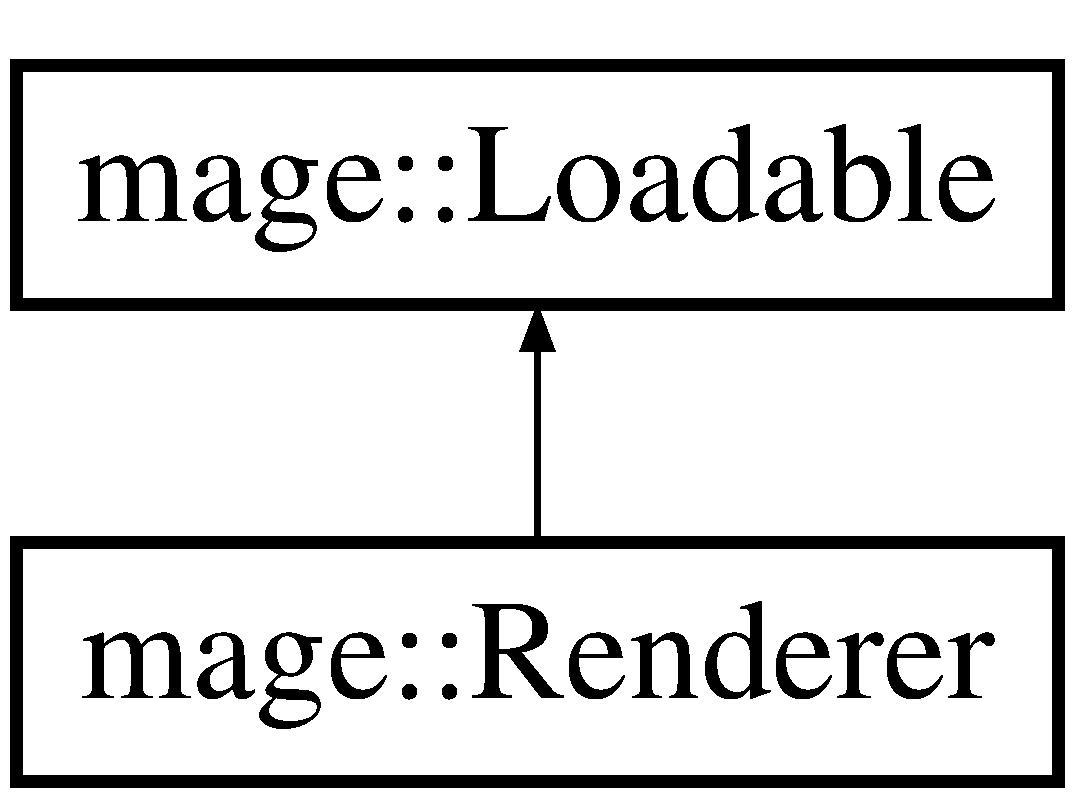
\includegraphics[height=2.000000cm]{classmage_1_1_renderer}
\end{center}
\end{figure}
\subsection*{Public Member Functions}
\begin{DoxyCompactItemize}
\item 
I\+D3\+D11\+Device2 $\ast$ \hyperlink{classmage_1_1_renderer_a38522d4b6933ef8f9ef5e46b713bdc95}{Get\+Device} ()
\item 
I\+D3\+D11\+Device\+Context2 $\ast$ \hyperlink{classmage_1_1_renderer_aa212ed67007115da62b6338f75e4eb75}{Get\+Device\+Context} ()
\item 
bool \hyperlink{classmage_1_1_renderer_a1de1804c1eedae7dc12435a520a10b9c}{Is\+Windowed} () const
\item 
bool \hyperlink{classmage_1_1_renderer_a5ae3220e19c68f47a8e4d55e3ced4694}{Is\+Full\+Screen} () const
\item 
bool \hyperlink{classmage_1_1_renderer_afdde83a1e2bc9288f000fb2575c525d0}{Lost\+Mode} () const
\item 
void \hyperlink{classmage_1_1_renderer_a9004ab608659188900c808eacb5f873c}{Switch\+Mode} (bool toggle)
\end{DoxyCompactItemize}
\subsection*{Protected Member Functions}
\begin{DoxyCompactItemize}
\item 
\hyperlink{classmage_1_1_renderer_a762dcda433c319af237d1dfd9bc6095f}{Renderer} (H\+W\+ND hwindow)
\item 
virtual \hyperlink{classmage_1_1_renderer_a997e041f28cc71d069d1ab7d29fe6ced}{$\sim$\+Renderer} ()
\item 
H\+R\+E\+S\+U\+LT \hyperlink{classmage_1_1_renderer_aafed50e7e14ca597541c091941351929}{Initialize\+Renderer} ()
\item 
H\+R\+E\+S\+U\+LT \hyperlink{classmage_1_1_renderer_a308beaf67b11128f02e87778b6a9c3c7}{Unitialize\+Renderer} ()
\item 
H\+R\+E\+S\+U\+LT \hyperlink{classmage_1_1_renderer_a4ee0187fb63587a219798523fb8cb7a6}{Setup\+Device} ()
\item 
H\+R\+E\+S\+U\+LT \hyperlink{classmage_1_1_renderer_af2aa545594936261bf2639e4e0814a83}{Setup\+Swap\+Chain} ()
\item 
H\+R\+E\+S\+U\+LT \hyperlink{classmage_1_1_renderer_afe99715a4ae6432ba561dcab048f79b4}{Setup\+Render\+Target\+View} ()
\item 
H\+R\+E\+S\+U\+LT \hyperlink{classmage_1_1_renderer_a95a34b64e815b0e5e95ce539bbd0f5a3}{Setup\+Depth\+Stencil\+View} ()
\item 
H\+R\+E\+S\+U\+LT \hyperlink{classmage_1_1_renderer_a9bc8598ccca5f6e7cf99010175b1360b}{Setup\+View\+Port} ()
\item 
void \hyperlink{classmage_1_1_renderer_a95ac55eb4cc79a5712a50bfb78f67fe6}{Render} (double elapsed\+\_\+time)
\end{DoxyCompactItemize}
\subsection*{Protected Attributes}
\begin{DoxyCompactItemize}
\item 
H\+W\+ND \hyperlink{classmage_1_1_renderer_afc314c8b146c3709edfd5349257a8387}{m\+\_\+hwindow}
\item 
D3\+D\+\_\+\+F\+E\+A\+T\+U\+R\+E\+\_\+\+L\+E\+V\+EL \hyperlink{classmage_1_1_renderer_aa97b108ef58f7d41ddb527f6ba2bfdf9}{m\+\_\+feature\+\_\+level}
\item 
I\+D3\+D11\+Device2 $\ast$ \hyperlink{classmage_1_1_renderer_a5af9d44e53bd523136cc52855a2dbe25}{m\+\_\+device2}
\item 
I\+D3\+D11\+Device\+Context2 $\ast$ \hyperlink{classmage_1_1_renderer_a57bee762f1a8c0ca13c62874a4297f48}{m\+\_\+device\+\_\+context2}
\item 
I\+D\+X\+G\+I\+Swap\+Chain2 $\ast$ \hyperlink{classmage_1_1_renderer_a64eb8b31f6835322d13e1d9b8ea9e113}{m\+\_\+swap\+\_\+chain2}
\item 
I\+D3\+D11\+Render\+Target\+View $\ast$ \hyperlink{classmage_1_1_renderer_a60eeb3b440c2c8a027b583ab93830d73}{m\+\_\+render\+\_\+target\+\_\+view}
\item 
I\+D3\+D11\+Texture2D $\ast$ \hyperlink{classmage_1_1_renderer_a1c19b2fb0347ab2e93f19d7a9d53a947}{m\+\_\+depth\+\_\+stencil}
\item 
I\+D3\+D11\+Depth\+Stencil\+View $\ast$ \hyperlink{classmage_1_1_renderer_a85b04ce9e3d0086c499910b2df82876d}{m\+\_\+depth\+\_\+stencil\+\_\+view}
\end{DoxyCompactItemize}
\subsection*{Private Attributes}
\begin{DoxyCompactItemize}
\item 
bool \hyperlink{classmage_1_1_renderer_a72bb88b17491bd388460afae9d207b0a}{m\+\_\+fullscreen}
\end{DoxyCompactItemize}
\subsection*{Friends}
\begin{DoxyCompactItemize}
\item 
class \hyperlink{classmage_1_1_renderer_a3e1914489e4bed4f9f23cdeab34a43dc}{Engine}
\end{DoxyCompactItemize}
\subsection*{Additional Inherited Members}


\subsection{Detailed Description}
A class of renderers. 

\subsection{Constructor \& Destructor Documentation}
\hypertarget{classmage_1_1_renderer_a762dcda433c319af237d1dfd9bc6095f}{}\label{classmage_1_1_renderer_a762dcda433c319af237d1dfd9bc6095f} 
\index{mage\+::\+Renderer@{mage\+::\+Renderer}!Renderer@{Renderer}}
\index{Renderer@{Renderer}!mage\+::\+Renderer@{mage\+::\+Renderer}}
\subsubsection{\texorpdfstring{Renderer()}{Renderer()}}
{\footnotesize\ttfamily mage\+::\+Renderer\+::\+Renderer (\begin{DoxyParamCaption}\item[{H\+W\+ND}]{hwindow }\end{DoxyParamCaption})\hspace{0.3cm}{\ttfamily [protected]}}

Constructs a renderer.


\begin{DoxyParams}[1]{Parameters}
\mbox{\tt in}  & {\em hwindow} & The main window handle. \\
\hline
\end{DoxyParams}
\hypertarget{classmage_1_1_renderer_a997e041f28cc71d069d1ab7d29fe6ced}{}\label{classmage_1_1_renderer_a997e041f28cc71d069d1ab7d29fe6ced} 
\index{mage\+::\+Renderer@{mage\+::\+Renderer}!````~Renderer@{$\sim$\+Renderer}}
\index{````~Renderer@{$\sim$\+Renderer}!mage\+::\+Renderer@{mage\+::\+Renderer}}
\subsubsection{\texorpdfstring{$\sim$\+Renderer()}{~Renderer()}}
{\footnotesize\ttfamily mage\+::\+Renderer\+::$\sim$\+Renderer (\begin{DoxyParamCaption}{ }\end{DoxyParamCaption})\hspace{0.3cm}{\ttfamily [protected]}, {\ttfamily [virtual]}}

Destructs this renderer. 

\subsection{Member Function Documentation}
\hypertarget{classmage_1_1_renderer_a38522d4b6933ef8f9ef5e46b713bdc95}{}\label{classmage_1_1_renderer_a38522d4b6933ef8f9ef5e46b713bdc95} 
\index{mage\+::\+Renderer@{mage\+::\+Renderer}!Get\+Device@{Get\+Device}}
\index{Get\+Device@{Get\+Device}!mage\+::\+Renderer@{mage\+::\+Renderer}}
\subsubsection{\texorpdfstring{Get\+Device()}{GetDevice()}}
{\footnotesize\ttfamily I\+D3\+D11\+Device2$\ast$ mage\+::\+Renderer\+::\+Get\+Device (\begin{DoxyParamCaption}{ }\end{DoxyParamCaption})}

Returns the device of this renderer.

\begin{DoxyReturn}{Returns}
A pointer to the device of this renderer. 
\end{DoxyReturn}
\hypertarget{classmage_1_1_renderer_aa212ed67007115da62b6338f75e4eb75}{}\label{classmage_1_1_renderer_aa212ed67007115da62b6338f75e4eb75} 
\index{mage\+::\+Renderer@{mage\+::\+Renderer}!Get\+Device\+Context@{Get\+Device\+Context}}
\index{Get\+Device\+Context@{Get\+Device\+Context}!mage\+::\+Renderer@{mage\+::\+Renderer}}
\subsubsection{\texorpdfstring{Get\+Device\+Context()}{GetDeviceContext()}}
{\footnotesize\ttfamily I\+D3\+D11\+Device\+Context2$\ast$ mage\+::\+Renderer\+::\+Get\+Device\+Context (\begin{DoxyParamCaption}{ }\end{DoxyParamCaption})}

Returns the device context of this renderer.

\begin{DoxyReturn}{Returns}
A pointer to the device context of this renderer. 
\end{DoxyReturn}
\hypertarget{classmage_1_1_renderer_aafed50e7e14ca597541c091941351929}{}\label{classmage_1_1_renderer_aafed50e7e14ca597541c091941351929} 
\index{mage\+::\+Renderer@{mage\+::\+Renderer}!Initialize\+Renderer@{Initialize\+Renderer}}
\index{Initialize\+Renderer@{Initialize\+Renderer}!mage\+::\+Renderer@{mage\+::\+Renderer}}
\subsubsection{\texorpdfstring{Initialize\+Renderer()}{InitializeRenderer()}}
{\footnotesize\ttfamily H\+R\+E\+S\+U\+LT mage\+::\+Renderer\+::\+Initialize\+Renderer (\begin{DoxyParamCaption}{ }\end{DoxyParamCaption})\hspace{0.3cm}{\ttfamily [protected]}}

Initializes this renderer.

\begin{DoxyReturn}{Returns}
A success/error value. 
\end{DoxyReturn}
\hypertarget{classmage_1_1_renderer_a5ae3220e19c68f47a8e4d55e3ced4694}{}\label{classmage_1_1_renderer_a5ae3220e19c68f47a8e4d55e3ced4694} 
\index{mage\+::\+Renderer@{mage\+::\+Renderer}!Is\+Full\+Screen@{Is\+Full\+Screen}}
\index{Is\+Full\+Screen@{Is\+Full\+Screen}!mage\+::\+Renderer@{mage\+::\+Renderer}}
\subsubsection{\texorpdfstring{Is\+Full\+Screen()}{IsFullScreen()}}
{\footnotesize\ttfamily bool mage\+::\+Renderer\+::\+Is\+Full\+Screen (\begin{DoxyParamCaption}{ }\end{DoxyParamCaption}) const}

Checks whether this renderer renders in full screen mode.

\begin{DoxyReturn}{Returns}
{\ttfamily true} if this renderer renders in full screen mode. {\ttfamily false} otherwise. 
\end{DoxyReturn}
\hypertarget{classmage_1_1_renderer_a1de1804c1eedae7dc12435a520a10b9c}{}\label{classmage_1_1_renderer_a1de1804c1eedae7dc12435a520a10b9c} 
\index{mage\+::\+Renderer@{mage\+::\+Renderer}!Is\+Windowed@{Is\+Windowed}}
\index{Is\+Windowed@{Is\+Windowed}!mage\+::\+Renderer@{mage\+::\+Renderer}}
\subsubsection{\texorpdfstring{Is\+Windowed()}{IsWindowed()}}
{\footnotesize\ttfamily bool mage\+::\+Renderer\+::\+Is\+Windowed (\begin{DoxyParamCaption}{ }\end{DoxyParamCaption}) const}

Checks whether this renderer renders in windowed mode.

\begin{DoxyReturn}{Returns}
{\ttfamily true} if this renderer renders in windowed mode. {\ttfamily false} otherwise. 
\end{DoxyReturn}
\hypertarget{classmage_1_1_renderer_afdde83a1e2bc9288f000fb2575c525d0}{}\label{classmage_1_1_renderer_afdde83a1e2bc9288f000fb2575c525d0} 
\index{mage\+::\+Renderer@{mage\+::\+Renderer}!Lost\+Mode@{Lost\+Mode}}
\index{Lost\+Mode@{Lost\+Mode}!mage\+::\+Renderer@{mage\+::\+Renderer}}
\subsubsection{\texorpdfstring{Lost\+Mode()}{LostMode()}}
{\footnotesize\ttfamily bool mage\+::\+Renderer\+::\+Lost\+Mode (\begin{DoxyParamCaption}{ }\end{DoxyParamCaption}) const}

Checks whether this renderer lost its mode, i.\+e. the current mode of this renderer differs from the cyrrent mode of its swap chain (due to for example A\+LT + T\+AB). \hypertarget{classmage_1_1_renderer_a95ac55eb4cc79a5712a50bfb78f67fe6}{}\label{classmage_1_1_renderer_a95ac55eb4cc79a5712a50bfb78f67fe6} 
\index{mage\+::\+Renderer@{mage\+::\+Renderer}!Render@{Render}}
\index{Render@{Render}!mage\+::\+Renderer@{mage\+::\+Renderer}}
\subsubsection{\texorpdfstring{Render()}{Render()}}
{\footnotesize\ttfamily void mage\+::\+Renderer\+::\+Render (\begin{DoxyParamCaption}\item[{double}]{elapsed\+\_\+time }\end{DoxyParamCaption})\hspace{0.3cm}{\ttfamily [protected]}}

Renders the current frame.


\begin{DoxyParams}[1]{Parameters}
\mbox{\tt in}  & {\em elapsed\+\_\+time} & The elapsed time since the previous frame. \\
\hline
\end{DoxyParams}
\hypertarget{classmage_1_1_renderer_a95a34b64e815b0e5e95ce539bbd0f5a3}{}\label{classmage_1_1_renderer_a95a34b64e815b0e5e95ce539bbd0f5a3} 
\index{mage\+::\+Renderer@{mage\+::\+Renderer}!Setup\+Depth\+Stencil\+View@{Setup\+Depth\+Stencil\+View}}
\index{Setup\+Depth\+Stencil\+View@{Setup\+Depth\+Stencil\+View}!mage\+::\+Renderer@{mage\+::\+Renderer}}
\subsubsection{\texorpdfstring{Setup\+Depth\+Stencil\+View()}{SetupDepthStencilView()}}
{\footnotesize\ttfamily H\+R\+E\+S\+U\+LT mage\+::\+Renderer\+::\+Setup\+Depth\+Stencil\+View (\begin{DoxyParamCaption}{ }\end{DoxyParamCaption})\hspace{0.3cm}{\ttfamily [protected]}}

Sets up the depth stencil view of this renderer.

\begin{DoxyReturn}{Returns}
A success/error value. 
\end{DoxyReturn}
\hypertarget{classmage_1_1_renderer_a4ee0187fb63587a219798523fb8cb7a6}{}\label{classmage_1_1_renderer_a4ee0187fb63587a219798523fb8cb7a6} 
\index{mage\+::\+Renderer@{mage\+::\+Renderer}!Setup\+Device@{Setup\+Device}}
\index{Setup\+Device@{Setup\+Device}!mage\+::\+Renderer@{mage\+::\+Renderer}}
\subsubsection{\texorpdfstring{Setup\+Device()}{SetupDevice()}}
{\footnotesize\ttfamily H\+R\+E\+S\+U\+LT mage\+::\+Renderer\+::\+Setup\+Device (\begin{DoxyParamCaption}{ }\end{DoxyParamCaption})\hspace{0.3cm}{\ttfamily [protected]}}

Setup the D3\+D11 device and context of this renderer.

\begin{DoxyReturn}{Returns}
A success/error value. 
\end{DoxyReturn}
\hypertarget{classmage_1_1_renderer_afe99715a4ae6432ba561dcab048f79b4}{}\label{classmage_1_1_renderer_afe99715a4ae6432ba561dcab048f79b4} 
\index{mage\+::\+Renderer@{mage\+::\+Renderer}!Setup\+Render\+Target\+View@{Setup\+Render\+Target\+View}}
\index{Setup\+Render\+Target\+View@{Setup\+Render\+Target\+View}!mage\+::\+Renderer@{mage\+::\+Renderer}}
\subsubsection{\texorpdfstring{Setup\+Render\+Target\+View()}{SetupRenderTargetView()}}
{\footnotesize\ttfamily H\+R\+E\+S\+U\+LT mage\+::\+Renderer\+::\+Setup\+Render\+Target\+View (\begin{DoxyParamCaption}{ }\end{DoxyParamCaption})\hspace{0.3cm}{\ttfamily [protected]}}

Sets up the render target view of this renderer.

\begin{DoxyReturn}{Returns}
A success/error value. 
\end{DoxyReturn}
\hypertarget{classmage_1_1_renderer_af2aa545594936261bf2639e4e0814a83}{}\label{classmage_1_1_renderer_af2aa545594936261bf2639e4e0814a83} 
\index{mage\+::\+Renderer@{mage\+::\+Renderer}!Setup\+Swap\+Chain@{Setup\+Swap\+Chain}}
\index{Setup\+Swap\+Chain@{Setup\+Swap\+Chain}!mage\+::\+Renderer@{mage\+::\+Renderer}}
\subsubsection{\texorpdfstring{Setup\+Swap\+Chain()}{SetupSwapChain()}}
{\footnotesize\ttfamily H\+R\+E\+S\+U\+LT mage\+::\+Renderer\+::\+Setup\+Swap\+Chain (\begin{DoxyParamCaption}{ }\end{DoxyParamCaption})\hspace{0.3cm}{\ttfamily [protected]}}

Sets up the swap chain of this renderer.

\begin{DoxyReturn}{Returns}
A success/error value. 
\end{DoxyReturn}
\hypertarget{classmage_1_1_renderer_a9bc8598ccca5f6e7cf99010175b1360b}{}\label{classmage_1_1_renderer_a9bc8598ccca5f6e7cf99010175b1360b} 
\index{mage\+::\+Renderer@{mage\+::\+Renderer}!Setup\+View\+Port@{Setup\+View\+Port}}
\index{Setup\+View\+Port@{Setup\+View\+Port}!mage\+::\+Renderer@{mage\+::\+Renderer}}
\subsubsection{\texorpdfstring{Setup\+View\+Port()}{SetupViewPort()}}
{\footnotesize\ttfamily H\+R\+E\+S\+U\+LT mage\+::\+Renderer\+::\+Setup\+View\+Port (\begin{DoxyParamCaption}{ }\end{DoxyParamCaption})\hspace{0.3cm}{\ttfamily [protected]}}

Sets up and binds the viewport of this renderer to the graphics pipeline.

\begin{DoxyReturn}{Returns}
A success/error value. 
\end{DoxyReturn}
\hypertarget{classmage_1_1_renderer_a9004ab608659188900c808eacb5f873c}{}\label{classmage_1_1_renderer_a9004ab608659188900c808eacb5f873c} 
\index{mage\+::\+Renderer@{mage\+::\+Renderer}!Switch\+Mode@{Switch\+Mode}}
\index{Switch\+Mode@{Switch\+Mode}!mage\+::\+Renderer@{mage\+::\+Renderer}}
\subsubsection{\texorpdfstring{Switch\+Mode()}{SwitchMode()}}
{\footnotesize\ttfamily void mage\+::\+Renderer\+::\+Switch\+Mode (\begin{DoxyParamCaption}\item[{bool}]{toggle }\end{DoxyParamCaption})}

Recreates the swap chain buffers and switches the mode of this renderer. Windowed mode is switched to full screen mode and vice versa.

\begin{DoxyReturn}{Returns}
toggle If {\ttfamily true} only the swap chain buffers will be recreated to match the current mode of the swap chain and no mode switch will occurs. If {\ttfamily false} both the swap chain buffers will be replaced and a mode switch will occur. 
\end{DoxyReturn}
\hypertarget{classmage_1_1_renderer_a308beaf67b11128f02e87778b6a9c3c7}{}\label{classmage_1_1_renderer_a308beaf67b11128f02e87778b6a9c3c7} 
\index{mage\+::\+Renderer@{mage\+::\+Renderer}!Unitialize\+Renderer@{Unitialize\+Renderer}}
\index{Unitialize\+Renderer@{Unitialize\+Renderer}!mage\+::\+Renderer@{mage\+::\+Renderer}}
\subsubsection{\texorpdfstring{Unitialize\+Renderer()}{UnitializeRenderer()}}
{\footnotesize\ttfamily H\+R\+E\+S\+U\+LT mage\+::\+Renderer\+::\+Unitialize\+Renderer (\begin{DoxyParamCaption}{ }\end{DoxyParamCaption})\hspace{0.3cm}{\ttfamily [protected]}}

Uninitializes this renderer.

\begin{DoxyReturn}{Returns}
A success/error value. 
\end{DoxyReturn}


\subsection{Friends And Related Function Documentation}
\hypertarget{classmage_1_1_renderer_a3e1914489e4bed4f9f23cdeab34a43dc}{}\label{classmage_1_1_renderer_a3e1914489e4bed4f9f23cdeab34a43dc} 
\index{mage\+::\+Renderer@{mage\+::\+Renderer}!Engine@{Engine}}
\index{Engine@{Engine}!mage\+::\+Renderer@{mage\+::\+Renderer}}
\subsubsection{\texorpdfstring{Engine}{Engine}}
{\footnotesize\ttfamily friend class \hyperlink{classmage_1_1_engine}{Engine}\hspace{0.3cm}{\ttfamily [friend]}}



\subsection{Member Data Documentation}
\hypertarget{classmage_1_1_renderer_a1c19b2fb0347ab2e93f19d7a9d53a947}{}\label{classmage_1_1_renderer_a1c19b2fb0347ab2e93f19d7a9d53a947} 
\index{mage\+::\+Renderer@{mage\+::\+Renderer}!m\+\_\+depth\+\_\+stencil@{m\+\_\+depth\+\_\+stencil}}
\index{m\+\_\+depth\+\_\+stencil@{m\+\_\+depth\+\_\+stencil}!mage\+::\+Renderer@{mage\+::\+Renderer}}
\subsubsection{\texorpdfstring{m\+\_\+depth\+\_\+stencil}{m\_depth\_stencil}}
{\footnotesize\ttfamily I\+D3\+D11\+Texture2D$\ast$ mage\+::\+Renderer\+::m\+\_\+depth\+\_\+stencil\hspace{0.3cm}{\ttfamily [protected]}}

\hypertarget{classmage_1_1_renderer_a85b04ce9e3d0086c499910b2df82876d}{}\label{classmage_1_1_renderer_a85b04ce9e3d0086c499910b2df82876d} 
\index{mage\+::\+Renderer@{mage\+::\+Renderer}!m\+\_\+depth\+\_\+stencil\+\_\+view@{m\+\_\+depth\+\_\+stencil\+\_\+view}}
\index{m\+\_\+depth\+\_\+stencil\+\_\+view@{m\+\_\+depth\+\_\+stencil\+\_\+view}!mage\+::\+Renderer@{mage\+::\+Renderer}}
\subsubsection{\texorpdfstring{m\+\_\+depth\+\_\+stencil\+\_\+view}{m\_depth\_stencil\_view}}
{\footnotesize\ttfamily I\+D3\+D11\+Depth\+Stencil\+View$\ast$ mage\+::\+Renderer\+::m\+\_\+depth\+\_\+stencil\+\_\+view\hspace{0.3cm}{\ttfamily [protected]}}

\hypertarget{classmage_1_1_renderer_a5af9d44e53bd523136cc52855a2dbe25}{}\label{classmage_1_1_renderer_a5af9d44e53bd523136cc52855a2dbe25} 
\index{mage\+::\+Renderer@{mage\+::\+Renderer}!m\+\_\+device2@{m\+\_\+device2}}
\index{m\+\_\+device2@{m\+\_\+device2}!mage\+::\+Renderer@{mage\+::\+Renderer}}
\subsubsection{\texorpdfstring{m\+\_\+device2}{m\_device2}}
{\footnotesize\ttfamily I\+D3\+D11\+Device2$\ast$ mage\+::\+Renderer\+::m\+\_\+device2\hspace{0.3cm}{\ttfamily [protected]}}

\hypertarget{classmage_1_1_renderer_a57bee762f1a8c0ca13c62874a4297f48}{}\label{classmage_1_1_renderer_a57bee762f1a8c0ca13c62874a4297f48} 
\index{mage\+::\+Renderer@{mage\+::\+Renderer}!m\+\_\+device\+\_\+context2@{m\+\_\+device\+\_\+context2}}
\index{m\+\_\+device\+\_\+context2@{m\+\_\+device\+\_\+context2}!mage\+::\+Renderer@{mage\+::\+Renderer}}
\subsubsection{\texorpdfstring{m\+\_\+device\+\_\+context2}{m\_device\_context2}}
{\footnotesize\ttfamily I\+D3\+D11\+Device\+Context2$\ast$ mage\+::\+Renderer\+::m\+\_\+device\+\_\+context2\hspace{0.3cm}{\ttfamily [protected]}}

\hypertarget{classmage_1_1_renderer_aa97b108ef58f7d41ddb527f6ba2bfdf9}{}\label{classmage_1_1_renderer_aa97b108ef58f7d41ddb527f6ba2bfdf9} 
\index{mage\+::\+Renderer@{mage\+::\+Renderer}!m\+\_\+feature\+\_\+level@{m\+\_\+feature\+\_\+level}}
\index{m\+\_\+feature\+\_\+level@{m\+\_\+feature\+\_\+level}!mage\+::\+Renderer@{mage\+::\+Renderer}}
\subsubsection{\texorpdfstring{m\+\_\+feature\+\_\+level}{m\_feature\_level}}
{\footnotesize\ttfamily D3\+D\+\_\+\+F\+E\+A\+T\+U\+R\+E\+\_\+\+L\+E\+V\+EL mage\+::\+Renderer\+::m\+\_\+feature\+\_\+level\hspace{0.3cm}{\ttfamily [protected]}}

\hypertarget{classmage_1_1_renderer_a72bb88b17491bd388460afae9d207b0a}{}\label{classmage_1_1_renderer_a72bb88b17491bd388460afae9d207b0a} 
\index{mage\+::\+Renderer@{mage\+::\+Renderer}!m\+\_\+fullscreen@{m\+\_\+fullscreen}}
\index{m\+\_\+fullscreen@{m\+\_\+fullscreen}!mage\+::\+Renderer@{mage\+::\+Renderer}}
\subsubsection{\texorpdfstring{m\+\_\+fullscreen}{m\_fullscreen}}
{\footnotesize\ttfamily bool mage\+::\+Renderer\+::m\+\_\+fullscreen\hspace{0.3cm}{\ttfamily [private]}}

A flag indicating whether this renderer uses a full screen mode (if {\ttfamily true}) or a windowed mode (if {\ttfamily false}). \hypertarget{classmage_1_1_renderer_afc314c8b146c3709edfd5349257a8387}{}\label{classmage_1_1_renderer_afc314c8b146c3709edfd5349257a8387} 
\index{mage\+::\+Renderer@{mage\+::\+Renderer}!m\+\_\+hwindow@{m\+\_\+hwindow}}
\index{m\+\_\+hwindow@{m\+\_\+hwindow}!mage\+::\+Renderer@{mage\+::\+Renderer}}
\subsubsection{\texorpdfstring{m\+\_\+hwindow}{m\_hwindow}}
{\footnotesize\ttfamily H\+W\+ND mage\+::\+Renderer\+::m\+\_\+hwindow\hspace{0.3cm}{\ttfamily [protected]}}

Main window handle of this renderer. \hypertarget{classmage_1_1_renderer_a60eeb3b440c2c8a027b583ab93830d73}{}\label{classmage_1_1_renderer_a60eeb3b440c2c8a027b583ab93830d73} 
\index{mage\+::\+Renderer@{mage\+::\+Renderer}!m\+\_\+render\+\_\+target\+\_\+view@{m\+\_\+render\+\_\+target\+\_\+view}}
\index{m\+\_\+render\+\_\+target\+\_\+view@{m\+\_\+render\+\_\+target\+\_\+view}!mage\+::\+Renderer@{mage\+::\+Renderer}}
\subsubsection{\texorpdfstring{m\+\_\+render\+\_\+target\+\_\+view}{m\_render\_target\_view}}
{\footnotesize\ttfamily I\+D3\+D11\+Render\+Target\+View$\ast$ mage\+::\+Renderer\+::m\+\_\+render\+\_\+target\+\_\+view\hspace{0.3cm}{\ttfamily [protected]}}

\hypertarget{classmage_1_1_renderer_a64eb8b31f6835322d13e1d9b8ea9e113}{}\label{classmage_1_1_renderer_a64eb8b31f6835322d13e1d9b8ea9e113} 
\index{mage\+::\+Renderer@{mage\+::\+Renderer}!m\+\_\+swap\+\_\+chain2@{m\+\_\+swap\+\_\+chain2}}
\index{m\+\_\+swap\+\_\+chain2@{m\+\_\+swap\+\_\+chain2}!mage\+::\+Renderer@{mage\+::\+Renderer}}
\subsubsection{\texorpdfstring{m\+\_\+swap\+\_\+chain2}{m\_swap\_chain2}}
{\footnotesize\ttfamily I\+D\+X\+G\+I\+Swap\+Chain2$\ast$ mage\+::\+Renderer\+::m\+\_\+swap\+\_\+chain2\hspace{0.3cm}{\ttfamily [protected]}}


\hypertarget{classmage_1_1_resource}{}\section{mage\+:\+:Resource Class Reference}
\label{classmage_1_1_resource}\index{mage\+::\+Resource@{mage\+::\+Resource}}


{\ttfamily \#include $<$resource.\+hpp$>$}

\subsection*{Public Member Functions}
\begin{DoxyCompactItemize}
\item 
\hyperlink{classmage_1_1_resource_a7b4febc86646d51ac116732af01abcaf}{Resource} (const string \&name, const string \&path=\char`\"{}./\char`\"{})
\item 
virtual \hyperlink{classmage_1_1_resource_a80112db991a7dfd1dc0b24967981ac60}{$\sim$\+Resource} ()
\item 
const string \& \hyperlink{classmage_1_1_resource_a77713b0c74f8983afc2d42843afe8cbe}{Get\+Name} () const
\item 
const string \& \hyperlink{classmage_1_1_resource_a2ef6c6937947b56cbabc569e3a63ca71}{Get\+Path} () const
\item 
const string \& \hyperlink{classmage_1_1_resource_a1e5163aed4ec9f73c477df2fe7ca2c03}{Get\+Filename} () const
\end{DoxyCompactItemize}
\subsection*{Private Member Functions}
\begin{DoxyCompactItemize}
\item 
uint32\+\_\+t \hyperlink{classmage_1_1_resource_a828bf8678979bfa92f2d2df81b60c57f}{Increment\+Reference\+Count} ()
\item 
uint32\+\_\+t \hyperlink{classmage_1_1_resource_a80b053a65f76bcb61ce9a81478277fc0}{Decrement\+Reference\+Count} ()
\end{DoxyCompactItemize}
\subsection*{Private Attributes}
\begin{DoxyCompactItemize}
\item 
const string \hyperlink{classmage_1_1_resource_a93019b74e9665195f1af17c60b6d171a}{m\+\_\+name}
\item 
const string \hyperlink{classmage_1_1_resource_a983470902250a8d16b6d5d01c332804b}{m\+\_\+path}
\item 
Atomic\+Int32 \hyperlink{classmage_1_1_resource_a7b54e6436afe7128383ab19172878cd9}{m\+\_\+reference\+\_\+count}
\end{DoxyCompactItemize}
\subsection*{Friends}
\begin{DoxyCompactItemize}
\item 
{\footnotesize template$<$typename T $>$ }\\class \hyperlink{classmage_1_1_resource_a51a7bf7c13d389aeee09c16059ca41c9}{Resource\+Manager}
\end{DoxyCompactItemize}


\subsection{Constructor \& Destructor Documentation}
\hypertarget{classmage_1_1_resource_a7b4febc86646d51ac116732af01abcaf}{}\label{classmage_1_1_resource_a7b4febc86646d51ac116732af01abcaf} 
\index{mage\+::\+Resource@{mage\+::\+Resource}!Resource@{Resource}}
\index{Resource@{Resource}!mage\+::\+Resource@{mage\+::\+Resource}}
\subsubsection{\texorpdfstring{Resource()}{Resource()}}
{\footnotesize\ttfamily mage\+::\+Resource\+::\+Resource (\begin{DoxyParamCaption}\item[{const string \&}]{name,  }\item[{const string \&}]{path = {\ttfamily \char`\"{}./\char`\"{}} }\end{DoxyParamCaption})}

\hypertarget{classmage_1_1_resource_a80112db991a7dfd1dc0b24967981ac60}{}\label{classmage_1_1_resource_a80112db991a7dfd1dc0b24967981ac60} 
\index{mage\+::\+Resource@{mage\+::\+Resource}!````~Resource@{$\sim$\+Resource}}
\index{````~Resource@{$\sim$\+Resource}!mage\+::\+Resource@{mage\+::\+Resource}}
\subsubsection{\texorpdfstring{$\sim$\+Resource()}{~Resource()}}
{\footnotesize\ttfamily virtual mage\+::\+Resource\+::$\sim$\+Resource (\begin{DoxyParamCaption}{ }\end{DoxyParamCaption})\hspace{0.3cm}{\ttfamily [virtual]}}



\subsection{Member Function Documentation}
\hypertarget{classmage_1_1_resource_a80b053a65f76bcb61ce9a81478277fc0}{}\label{classmage_1_1_resource_a80b053a65f76bcb61ce9a81478277fc0} 
\index{mage\+::\+Resource@{mage\+::\+Resource}!Decrement\+Reference\+Count@{Decrement\+Reference\+Count}}
\index{Decrement\+Reference\+Count@{Decrement\+Reference\+Count}!mage\+::\+Resource@{mage\+::\+Resource}}
\subsubsection{\texorpdfstring{Decrement\+Reference\+Count()}{DecrementReferenceCount()}}
{\footnotesize\ttfamily uint32\+\_\+t mage\+::\+Resource\+::\+Decrement\+Reference\+Count (\begin{DoxyParamCaption}{ }\end{DoxyParamCaption})\hspace{0.3cm}{\ttfamily [private]}}

\hypertarget{classmage_1_1_resource_a1e5163aed4ec9f73c477df2fe7ca2c03}{}\label{classmage_1_1_resource_a1e5163aed4ec9f73c477df2fe7ca2c03} 
\index{mage\+::\+Resource@{mage\+::\+Resource}!Get\+Filename@{Get\+Filename}}
\index{Get\+Filename@{Get\+Filename}!mage\+::\+Resource@{mage\+::\+Resource}}
\subsubsection{\texorpdfstring{Get\+Filename()}{GetFilename()}}
{\footnotesize\ttfamily const string\& mage\+::\+Resource\+::\+Get\+Filename (\begin{DoxyParamCaption}{ }\end{DoxyParamCaption}) const}

\hypertarget{classmage_1_1_resource_a77713b0c74f8983afc2d42843afe8cbe}{}\label{classmage_1_1_resource_a77713b0c74f8983afc2d42843afe8cbe} 
\index{mage\+::\+Resource@{mage\+::\+Resource}!Get\+Name@{Get\+Name}}
\index{Get\+Name@{Get\+Name}!mage\+::\+Resource@{mage\+::\+Resource}}
\subsubsection{\texorpdfstring{Get\+Name()}{GetName()}}
{\footnotesize\ttfamily const string\& mage\+::\+Resource\+::\+Get\+Name (\begin{DoxyParamCaption}{ }\end{DoxyParamCaption}) const}

\hypertarget{classmage_1_1_resource_a2ef6c6937947b56cbabc569e3a63ca71}{}\label{classmage_1_1_resource_a2ef6c6937947b56cbabc569e3a63ca71} 
\index{mage\+::\+Resource@{mage\+::\+Resource}!Get\+Path@{Get\+Path}}
\index{Get\+Path@{Get\+Path}!mage\+::\+Resource@{mage\+::\+Resource}}
\subsubsection{\texorpdfstring{Get\+Path()}{GetPath()}}
{\footnotesize\ttfamily const string\& mage\+::\+Resource\+::\+Get\+Path (\begin{DoxyParamCaption}{ }\end{DoxyParamCaption}) const}

\hypertarget{classmage_1_1_resource_a828bf8678979bfa92f2d2df81b60c57f}{}\label{classmage_1_1_resource_a828bf8678979bfa92f2d2df81b60c57f} 
\index{mage\+::\+Resource@{mage\+::\+Resource}!Increment\+Reference\+Count@{Increment\+Reference\+Count}}
\index{Increment\+Reference\+Count@{Increment\+Reference\+Count}!mage\+::\+Resource@{mage\+::\+Resource}}
\subsubsection{\texorpdfstring{Increment\+Reference\+Count()}{IncrementReferenceCount()}}
{\footnotesize\ttfamily uint32\+\_\+t mage\+::\+Resource\+::\+Increment\+Reference\+Count (\begin{DoxyParamCaption}{ }\end{DoxyParamCaption})\hspace{0.3cm}{\ttfamily [private]}}



\subsection{Friends And Related Function Documentation}
\hypertarget{classmage_1_1_resource_a51a7bf7c13d389aeee09c16059ca41c9}{}\label{classmage_1_1_resource_a51a7bf7c13d389aeee09c16059ca41c9} 
\index{mage\+::\+Resource@{mage\+::\+Resource}!Resource\+Manager@{Resource\+Manager}}
\index{Resource\+Manager@{Resource\+Manager}!mage\+::\+Resource@{mage\+::\+Resource}}
\subsubsection{\texorpdfstring{Resource\+Manager}{ResourceManager}}
{\footnotesize\ttfamily template$<$typename T $>$ \\
friend class \hyperlink{classmage_1_1_resource_manager}{Resource\+Manager}\hspace{0.3cm}{\ttfamily [friend]}}



\subsection{Member Data Documentation}
\hypertarget{classmage_1_1_resource_a93019b74e9665195f1af17c60b6d171a}{}\label{classmage_1_1_resource_a93019b74e9665195f1af17c60b6d171a} 
\index{mage\+::\+Resource@{mage\+::\+Resource}!m\+\_\+name@{m\+\_\+name}}
\index{m\+\_\+name@{m\+\_\+name}!mage\+::\+Resource@{mage\+::\+Resource}}
\subsubsection{\texorpdfstring{m\+\_\+name}{m\_name}}
{\footnotesize\ttfamily const string mage\+::\+Resource\+::m\+\_\+name\hspace{0.3cm}{\ttfamily [private]}}

\hypertarget{classmage_1_1_resource_a983470902250a8d16b6d5d01c332804b}{}\label{classmage_1_1_resource_a983470902250a8d16b6d5d01c332804b} 
\index{mage\+::\+Resource@{mage\+::\+Resource}!m\+\_\+path@{m\+\_\+path}}
\index{m\+\_\+path@{m\+\_\+path}!mage\+::\+Resource@{mage\+::\+Resource}}
\subsubsection{\texorpdfstring{m\+\_\+path}{m\_path}}
{\footnotesize\ttfamily const string mage\+::\+Resource\+::m\+\_\+path\hspace{0.3cm}{\ttfamily [private]}}

\hypertarget{classmage_1_1_resource_a7b54e6436afe7128383ab19172878cd9}{}\label{classmage_1_1_resource_a7b54e6436afe7128383ab19172878cd9} 
\index{mage\+::\+Resource@{mage\+::\+Resource}!m\+\_\+reference\+\_\+count@{m\+\_\+reference\+\_\+count}}
\index{m\+\_\+reference\+\_\+count@{m\+\_\+reference\+\_\+count}!mage\+::\+Resource@{mage\+::\+Resource}}
\subsubsection{\texorpdfstring{m\+\_\+reference\+\_\+count}{m\_reference\_count}}
{\footnotesize\ttfamily Atomic\+Int32 mage\+::\+Resource\+::m\+\_\+reference\+\_\+count\hspace{0.3cm}{\ttfamily [private]}}


\hypertarget{classmage_1_1_resource_manager}{}\section{mage\+:\+:Resource\+Manager$<$ T $>$ Class Template Reference}
\label{classmage_1_1_resource_manager}\index{mage\+::\+Resource\+Manager$<$ T $>$@{mage\+::\+Resource\+Manager$<$ T $>$}}


{\ttfamily \#include $<$resource\+\_\+manager.\+hpp$>$}

\subsection*{Public Member Functions}
\begin{DoxyCompactItemize}
\item 
\hyperlink{classmage_1_1_resource_manager_ab8596e3f3c9fa2eb693cf4cc9aeb95d9}{Resource\+Manager} (void($\ast$Create\+Resource\+Function)(T $\ast$$\ast$resource, const wstring \&name, const wstring \&path)=nullptr)
\item 
virtual \hyperlink{classmage_1_1_resource_manager_a60685932f6c5f40333cd1e072a6f8c81}{$\sim$\+Resource\+Manager} ()=default
\item 
bool \hyperlink{classmage_1_1_resource_manager_a3ce8e6eef6c07dc672306271d2274ff6}{Contains\+Resource} (const wstring \&name, const wstring \&path=\char`\"{}./\char`\"{}) const
\item 
size\+\_\+t \hyperlink{classmage_1_1_resource_manager_a1872b087dac1794746b320c6ece63fd8}{Get\+Numberb\+Of\+Resources} () const
\item 
\hyperlink{namespacemage_a1e01ae66713838a7a67d30e44c67703e}{Shared\+Ptr}$<$ T $>$ \hyperlink{classmage_1_1_resource_manager_a97e20a40abfebc7709ddd51d78f991b9}{Add\+Resource} (const wstring \&name, const wstring \&path=\char`\"{}./\char`\"{})
\item 
void \hyperlink{classmage_1_1_resource_manager_ac557e5047590d0403291557c88966574}{Remove\+Resource} (\hyperlink{namespacemage_a1e01ae66713838a7a67d30e44c67703e}{Shared\+Ptr}$<$ T $>$ resource)
\item 
void \hyperlink{classmage_1_1_resource_manager_a1d9f7a5dfbf75c3c8d09c2130bee11f1}{Remove\+Resource} (const wstring \&name, const wstring \&path=\char`\"{}./\char`\"{})
\item 
\hyperlink{namespacemage_a1e01ae66713838a7a67d30e44c67703e}{Shared\+Ptr}$<$ T $>$ \hyperlink{classmage_1_1_resource_manager_a7632144a5d65ba34b9d1923b9201f129}{Get\+Resource} (const wstring \&name, const wstring \&path=\char`\"{}./\char`\"{}) const
\end{DoxyCompactItemize}
\subsection*{Private Member Functions}
\begin{DoxyCompactItemize}
\item 
\hyperlink{classmage_1_1_resource_manager_a3b424e1ef7f543a2705d1124018d9921}{Resource\+Manager} (const \hyperlink{classmage_1_1_resource_manager}{Resource\+Manager} \&resource\+\_\+manager)=delete
\item 
\hyperlink{classmage_1_1_resource_manager}{Resource\+Manager} \& \hyperlink{classmage_1_1_resource_manager_a5cc1867dbb196671fb53763c98aee1dd}{operator=} (const \hyperlink{classmage_1_1_resource_manager}{Resource\+Manager} \&resource\+\_\+manager)=delete
\end{DoxyCompactItemize}
\subsection*{Private Attributes}
\begin{DoxyCompactItemize}
\item 
map$<$ wstring, \hyperlink{namespacemage_a1e01ae66713838a7a67d30e44c67703e}{Shared\+Ptr}$<$ T $>$ $>$ \hyperlink{classmage_1_1_resource_manager_a7d5f31a34e76f343988b7d6e9a62a617}{m\+\_\+resources}
\item 
void($\ast$ \hyperlink{classmage_1_1_resource_manager_a41d5a40aeaef12e2ecef0cb8f5f4a4d5}{Create\+Resource} )(T $\ast$$\ast$resource, const wstring \&name, const wstring \&path)
\end{DoxyCompactItemize}


\subsection{Detailed Description}
\subsubsection*{template$<$typename T$>$\newline
class mage\+::\+Resource\+Manager$<$ T $>$}

A class of resource managers.


\begin{DoxyTemplParams}{Template Parameters}
{\em T} & The type of resources. \\
\hline
\end{DoxyTemplParams}


\subsection{Constructor \& Destructor Documentation}
\hypertarget{classmage_1_1_resource_manager_ab8596e3f3c9fa2eb693cf4cc9aeb95d9}{}\label{classmage_1_1_resource_manager_ab8596e3f3c9fa2eb693cf4cc9aeb95d9} 
\index{mage\+::\+Resource\+Manager@{mage\+::\+Resource\+Manager}!Resource\+Manager@{Resource\+Manager}}
\index{Resource\+Manager@{Resource\+Manager}!mage\+::\+Resource\+Manager@{mage\+::\+Resource\+Manager}}
\subsubsection{\texorpdfstring{Resource\+Manager()}{ResourceManager()}\hspace{0.1cm}{\footnotesize\ttfamily [1/2]}}
{\footnotesize\ttfamily template$<$typename T $>$ \\
\hyperlink{classmage_1_1_resource_manager}{mage\+::\+Resource\+Manager}$<$ T $>$\+::\hyperlink{classmage_1_1_resource_manager}{Resource\+Manager} (\begin{DoxyParamCaption}\item[{void($\ast$)(T $\ast$$\ast$resource, const wstring \&name, const wstring \&path)}]{Create\+Resource\+Function = {\ttfamily nullptr} }\end{DoxyParamCaption})}

Constructs a resource manager.


\begin{DoxyParams}[1]{Parameters}
\mbox{\tt in}  & {\em Create\+Resource\+Function} & The application specific resource creation function. \\
\hline
\end{DoxyParams}
\hypertarget{classmage_1_1_resource_manager_a60685932f6c5f40333cd1e072a6f8c81}{}\label{classmage_1_1_resource_manager_a60685932f6c5f40333cd1e072a6f8c81} 
\index{mage\+::\+Resource\+Manager@{mage\+::\+Resource\+Manager}!````~Resource\+Manager@{$\sim$\+Resource\+Manager}}
\index{````~Resource\+Manager@{$\sim$\+Resource\+Manager}!mage\+::\+Resource\+Manager@{mage\+::\+Resource\+Manager}}
\subsubsection{\texorpdfstring{$\sim$\+Resource\+Manager()}{~ResourceManager()}}
{\footnotesize\ttfamily template$<$typename T $>$ \\
virtual \hyperlink{classmage_1_1_resource_manager}{mage\+::\+Resource\+Manager}$<$ T $>$\+::$\sim$\hyperlink{classmage_1_1_resource_manager}{Resource\+Manager} (\begin{DoxyParamCaption}{ }\end{DoxyParamCaption})\hspace{0.3cm}{\ttfamily [virtual]}, {\ttfamily [default]}}

Destructs this resource manager. \hypertarget{classmage_1_1_resource_manager_a3b424e1ef7f543a2705d1124018d9921}{}\label{classmage_1_1_resource_manager_a3b424e1ef7f543a2705d1124018d9921} 
\index{mage\+::\+Resource\+Manager@{mage\+::\+Resource\+Manager}!Resource\+Manager@{Resource\+Manager}}
\index{Resource\+Manager@{Resource\+Manager}!mage\+::\+Resource\+Manager@{mage\+::\+Resource\+Manager}}
\subsubsection{\texorpdfstring{Resource\+Manager()}{ResourceManager()}\hspace{0.1cm}{\footnotesize\ttfamily [2/2]}}
{\footnotesize\ttfamily template$<$typename T $>$ \\
\hyperlink{classmage_1_1_resource_manager}{mage\+::\+Resource\+Manager}$<$ T $>$\+::\hyperlink{classmage_1_1_resource_manager}{Resource\+Manager} (\begin{DoxyParamCaption}\item[{const \hyperlink{classmage_1_1_resource_manager}{Resource\+Manager}$<$ T $>$ \&}]{resource\+\_\+manager }\end{DoxyParamCaption})\hspace{0.3cm}{\ttfamily [private]}, {\ttfamily [delete]}}

Constructs a resource manager from the given resource manager.


\begin{DoxyParams}[1]{Parameters}
\mbox{\tt in}  & {\em resource\+\_\+manager} & A reference to the resource manager. \\
\hline
\end{DoxyParams}


\subsection{Member Function Documentation}
\hypertarget{classmage_1_1_resource_manager_a97e20a40abfebc7709ddd51d78f991b9}{}\label{classmage_1_1_resource_manager_a97e20a40abfebc7709ddd51d78f991b9} 
\index{mage\+::\+Resource\+Manager@{mage\+::\+Resource\+Manager}!Add\+Resource@{Add\+Resource}}
\index{Add\+Resource@{Add\+Resource}!mage\+::\+Resource\+Manager@{mage\+::\+Resource\+Manager}}
\subsubsection{\texorpdfstring{Add\+Resource()}{AddResource()}}
{\footnotesize\ttfamily template$<$typename T $>$ \\
\hyperlink{namespacemage_a1e01ae66713838a7a67d30e44c67703e}{Shared\+Ptr}$<$ T $>$ \hyperlink{classmage_1_1_resource_manager}{mage\+::\+Resource\+Manager}$<$ T $>$\+::Add\+Resource (\begin{DoxyParamCaption}\item[{const wstring \&}]{name,  }\item[{const wstring \&}]{path = {\ttfamily \char`\"{}./\char`\"{}} }\end{DoxyParamCaption})}

Adds a new resource to this resource manager.


\begin{DoxyParams}[1]{Parameters}
\mbox{\tt in}  & {\em name} & A reference to the name of the new resource. \\
\hline
\mbox{\tt in}  & {\em path} & A reference to the path of the new resource. \\
\hline
\end{DoxyParams}
\begin{DoxyReturn}{Returns}
A pointer to the resource. 
\end{DoxyReturn}
\hypertarget{classmage_1_1_resource_manager_a3ce8e6eef6c07dc672306271d2274ff6}{}\label{classmage_1_1_resource_manager_a3ce8e6eef6c07dc672306271d2274ff6} 
\index{mage\+::\+Resource\+Manager@{mage\+::\+Resource\+Manager}!Contains\+Resource@{Contains\+Resource}}
\index{Contains\+Resource@{Contains\+Resource}!mage\+::\+Resource\+Manager@{mage\+::\+Resource\+Manager}}
\subsubsection{\texorpdfstring{Contains\+Resource()}{ContainsResource()}}
{\footnotesize\ttfamily template$<$typename T $>$ \\
bool \hyperlink{classmage_1_1_resource_manager}{mage\+::\+Resource\+Manager}$<$ T $>$\+::Contains\+Resource (\begin{DoxyParamCaption}\item[{const wstring \&}]{name,  }\item[{const wstring \&}]{path = {\ttfamily \char`\"{}./\char`\"{}} }\end{DoxyParamCaption}) const}

Checks whether this resource manager contains the given resource.


\begin{DoxyParams}[1]{Parameters}
\mbox{\tt in}  & {\em name} & A reference to the name of the resource. \\
\hline
\mbox{\tt in}  & {\em path} & A reference to the path of the resource. \\
\hline
\end{DoxyParams}
\begin{DoxyReturn}{Returns}
{\ttfamily true} if this resource manager contains the given resource. {\ttfamily false} otherwise. 
\end{DoxyReturn}
\hypertarget{classmage_1_1_resource_manager_a1872b087dac1794746b320c6ece63fd8}{}\label{classmage_1_1_resource_manager_a1872b087dac1794746b320c6ece63fd8} 
\index{mage\+::\+Resource\+Manager@{mage\+::\+Resource\+Manager}!Get\+Numberb\+Of\+Resources@{Get\+Numberb\+Of\+Resources}}
\index{Get\+Numberb\+Of\+Resources@{Get\+Numberb\+Of\+Resources}!mage\+::\+Resource\+Manager@{mage\+::\+Resource\+Manager}}
\subsubsection{\texorpdfstring{Get\+Numberb\+Of\+Resources()}{GetNumberbOfResources()}}
{\footnotesize\ttfamily template$<$typename T $>$ \\
size\+\_\+t \hyperlink{classmage_1_1_resource_manager}{mage\+::\+Resource\+Manager}$<$ T $>$\+::Get\+Numberb\+Of\+Resources (\begin{DoxyParamCaption}{ }\end{DoxyParamCaption}) const}

Returns the number of resources of this resource manager.

\begin{DoxyReturn}{Returns}
The number of resources of this resource manager. 
\end{DoxyReturn}
\hypertarget{classmage_1_1_resource_manager_a7632144a5d65ba34b9d1923b9201f129}{}\label{classmage_1_1_resource_manager_a7632144a5d65ba34b9d1923b9201f129} 
\index{mage\+::\+Resource\+Manager@{mage\+::\+Resource\+Manager}!Get\+Resource@{Get\+Resource}}
\index{Get\+Resource@{Get\+Resource}!mage\+::\+Resource\+Manager@{mage\+::\+Resource\+Manager}}
\subsubsection{\texorpdfstring{Get\+Resource()}{GetResource()}}
{\footnotesize\ttfamily template$<$typename T $>$ \\
\hyperlink{namespacemage_a1e01ae66713838a7a67d30e44c67703e}{Shared\+Ptr}$<$ T $>$ \hyperlink{classmage_1_1_resource_manager}{mage\+::\+Resource\+Manager}$<$ T $>$\+::Get\+Resource (\begin{DoxyParamCaption}\item[{const wstring \&}]{name,  }\item[{const wstring \&}]{path = {\ttfamily \char`\"{}./\char`\"{}} }\end{DoxyParamCaption}) const}

Returns a resource of this resource manager by its filename (given name and path).


\begin{DoxyParams}[1]{Parameters}
\mbox{\tt in}  & {\em name} & A reference to the name of the resource. \\
\hline
\mbox{\tt in}  & {\em path} & A reference to the path of the resource. \\
\hline
\end{DoxyParams}
\begin{DoxyReturn}{Returns}
{\ttfamily nullptr} if the resource is not present. 

A pointer to the resource. 
\end{DoxyReturn}
\hypertarget{classmage_1_1_resource_manager_a5cc1867dbb196671fb53763c98aee1dd}{}\label{classmage_1_1_resource_manager_a5cc1867dbb196671fb53763c98aee1dd} 
\index{mage\+::\+Resource\+Manager@{mage\+::\+Resource\+Manager}!operator=@{operator=}}
\index{operator=@{operator=}!mage\+::\+Resource\+Manager@{mage\+::\+Resource\+Manager}}
\subsubsection{\texorpdfstring{operator=()}{operator=()}}
{\footnotesize\ttfamily template$<$typename T $>$ \\
\hyperlink{classmage_1_1_resource_manager}{Resource\+Manager}\& \hyperlink{classmage_1_1_resource_manager}{mage\+::\+Resource\+Manager}$<$ T $>$\+::operator= (\begin{DoxyParamCaption}\item[{const \hyperlink{classmage_1_1_resource_manager}{Resource\+Manager}$<$ T $>$ \&}]{resource\+\_\+manager }\end{DoxyParamCaption})\hspace{0.3cm}{\ttfamily [private]}, {\ttfamily [delete]}}

Copies the given resource manager to this resource manager.


\begin{DoxyParams}[1]{Parameters}
\mbox{\tt in}  & {\em resource\+\_\+manager} & A reference to the resource manager to copy from. \\
\hline
\end{DoxyParams}
\begin{DoxyReturn}{Returns}
A reference to the copy of the given resource manager (i.\+e. this resource manager). 
\end{DoxyReturn}
\hypertarget{classmage_1_1_resource_manager_ac557e5047590d0403291557c88966574}{}\label{classmage_1_1_resource_manager_ac557e5047590d0403291557c88966574} 
\index{mage\+::\+Resource\+Manager@{mage\+::\+Resource\+Manager}!Remove\+Resource@{Remove\+Resource}}
\index{Remove\+Resource@{Remove\+Resource}!mage\+::\+Resource\+Manager@{mage\+::\+Resource\+Manager}}
\subsubsection{\texorpdfstring{Remove\+Resource()}{RemoveResource()}\hspace{0.1cm}{\footnotesize\ttfamily [1/2]}}
{\footnotesize\ttfamily template$<$typename T $>$ \\
void \hyperlink{classmage_1_1_resource_manager}{mage\+::\+Resource\+Manager}$<$ T $>$\+::Remove\+Resource (\begin{DoxyParamCaption}\item[{\hyperlink{namespacemage_a1e01ae66713838a7a67d30e44c67703e}{Shared\+Ptr}$<$ T $>$}]{resource }\end{DoxyParamCaption})}

Removes the given resource from this resource manager.


\begin{DoxyParams}[1]{Parameters}
\mbox{\tt in}  & {\em resource} & A pointer to the resource. \\
\hline
\end{DoxyParams}
\hypertarget{classmage_1_1_resource_manager_a1d9f7a5dfbf75c3c8d09c2130bee11f1}{}\label{classmage_1_1_resource_manager_a1d9f7a5dfbf75c3c8d09c2130bee11f1} 
\index{mage\+::\+Resource\+Manager@{mage\+::\+Resource\+Manager}!Remove\+Resource@{Remove\+Resource}}
\index{Remove\+Resource@{Remove\+Resource}!mage\+::\+Resource\+Manager@{mage\+::\+Resource\+Manager}}
\subsubsection{\texorpdfstring{Remove\+Resource()}{RemoveResource()}\hspace{0.1cm}{\footnotesize\ttfamily [2/2]}}
{\footnotesize\ttfamily template$<$typename T $>$ \\
void \hyperlink{classmage_1_1_resource_manager}{mage\+::\+Resource\+Manager}$<$ T $>$\+::Remove\+Resource (\begin{DoxyParamCaption}\item[{const wstring \&}]{name,  }\item[{const wstring \&}]{path = {\ttfamily \char`\"{}./\char`\"{}} }\end{DoxyParamCaption})}

Removes the given resource from this resource manager.


\begin{DoxyParams}[1]{Parameters}
\mbox{\tt in}  & {\em name} & A reference to the name of the resource. \\
\hline
\mbox{\tt in}  & {\em path} & A reference to the path of the resource. \\
\hline
\end{DoxyParams}


\subsection{Member Data Documentation}
\hypertarget{classmage_1_1_resource_manager_a41d5a40aeaef12e2ecef0cb8f5f4a4d5}{}\label{classmage_1_1_resource_manager_a41d5a40aeaef12e2ecef0cb8f5f4a4d5} 
\index{mage\+::\+Resource\+Manager@{mage\+::\+Resource\+Manager}!Create\+Resource@{Create\+Resource}}
\index{Create\+Resource@{Create\+Resource}!mage\+::\+Resource\+Manager@{mage\+::\+Resource\+Manager}}
\subsubsection{\texorpdfstring{Create\+Resource}{CreateResource}}
{\footnotesize\ttfamily template$<$typename T $>$ \\
void($\ast$ \hyperlink{classmage_1_1_resource_manager}{mage\+::\+Resource\+Manager}$<$ T $>$\+::Create\+Resource) (T $\ast$$\ast$resource, const wstring \&name, const wstring \&path)\hspace{0.3cm}{\ttfamily [private]}}

The application specific resource creation function for the resources of this resource manager. \hypertarget{classmage_1_1_resource_manager_a7d5f31a34e76f343988b7d6e9a62a617}{}\label{classmage_1_1_resource_manager_a7d5f31a34e76f343988b7d6e9a62a617} 
\index{mage\+::\+Resource\+Manager@{mage\+::\+Resource\+Manager}!m\+\_\+resources@{m\+\_\+resources}}
\index{m\+\_\+resources@{m\+\_\+resources}!mage\+::\+Resource\+Manager@{mage\+::\+Resource\+Manager}}
\subsubsection{\texorpdfstring{m\+\_\+resources}{m\_resources}}
{\footnotesize\ttfamily template$<$typename T $>$ \\
map$<$ wstring, \hyperlink{namespacemage_a1e01ae66713838a7a67d30e44c67703e}{Shared\+Ptr}$<$ T $>$ $>$ \hyperlink{classmage_1_1_resource_manager}{mage\+::\+Resource\+Manager}$<$ T $>$\+::m\+\_\+resources\hspace{0.3cm}{\ttfamily [private]}}

The map containing the resources of this resource manager as value and their file names as key. 
\hypertarget{classmage_1_1_scene_node}{}\section{mage\+:\+:Scene\+Node Class Reference}
\label{classmage_1_1_scene_node}\index{mage\+::\+Scene\+Node@{mage\+::\+Scene\+Node}}


{\ttfamily \#include $<$scene\+\_\+node.\+hpp$>$}

Inheritance diagram for mage\+:\+:Scene\+Node\+:\begin{figure}[H]
\begin{center}
\leavevmode
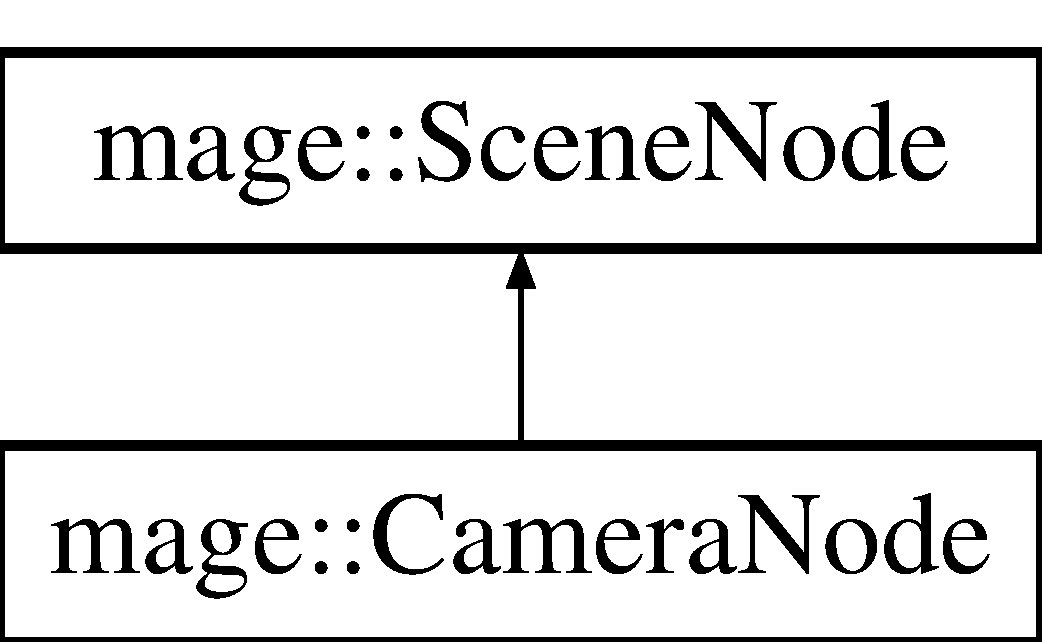
\includegraphics[height=2.000000cm]{classmage_1_1_scene_node}
\end{center}
\end{figure}
\subsection*{Public Member Functions}
\begin{DoxyCompactItemize}
\item 
virtual \hyperlink{classmage_1_1_scene_node_ad7ae54e25fb970772c0b0a6c5bac57ff}{$\sim$\+Scene\+Node} ()
\item 
\hyperlink{classmage_1_1_scene_node}{Scene\+Node} $\ast$ \hyperlink{classmage_1_1_scene_node_a512a9d0f935abf304980312680be3f30}{Get\+Parent} () const
\item 
bool \hyperlink{classmage_1_1_scene_node_a99c86a1d18b41d4c5ce0384ba53a0952}{Contains\+Child} (const \hyperlink{classmage_1_1_scene_node}{Scene\+Node} $\ast$child) const
\item 
void \hyperlink{classmage_1_1_scene_node_ac07f89af783b1658a1f74205914f6fa3}{Add\+Child} (\hyperlink{classmage_1_1_scene_node}{Scene\+Node} $\ast$child)
\item 
void \hyperlink{classmage_1_1_scene_node_a42aa6487f21c948ab7ce6f64a57e5f11}{Remove\+Child} (\hyperlink{classmage_1_1_scene_node}{Scene\+Node} $\ast$child)
\item 
size\+\_\+t \hyperlink{classmage_1_1_scene_node_a99c5eb3c253a2e620bd85ac845d3bb77}{Get\+Nb\+Of\+Childs} () const
\item 
\hyperlink{structmage_1_1_transform}{Transform} \& \hyperlink{classmage_1_1_scene_node_a72bfe51e9f233dd35fd8affd24b0a67a}{Get\+Transform} ()
\item 
const \hyperlink{structmage_1_1_transform}{Transform} \& \hyperlink{classmage_1_1_scene_node_ab68ffa4886e8e5ff9757362823a1aa74}{Get\+Transform} () const
\item 
X\+M\+M\+A\+T\+R\+IX \hyperlink{classmage_1_1_scene_node_a5ec8b0d2e5ba7873842c0fa65e1248bb}{Get\+Parent\+To\+Object\+Matrix} () const
\item 
X\+M\+M\+A\+T\+R\+IX \hyperlink{classmage_1_1_scene_node_afb199589e809c3cb0e46a691a737e5da}{Get\+Parent\+To\+World\+Matrix} () const
\item 
X\+M\+M\+A\+T\+R\+IX \hyperlink{classmage_1_1_scene_node_a0ddba0d70a8b2ce0ef80f25673d0dd56}{Get\+World\+To\+Object\+Matrix} () const
\item 
X\+M\+M\+A\+T\+R\+IX \hyperlink{classmage_1_1_scene_node_a4325660d42f5f393c77389a44aedb5cb}{Get\+Object\+To\+World\+Matrix} () const
\item 
virtual void \hyperlink{classmage_1_1_scene_node_a32ed8763c8f8b4caa155f64551d96f13}{Accept} (\hyperlink{classmage_1_1_scene_node_visitor}{Scene\+Node\+Visitor} \&visitor)=0
\item 
virtual void \hyperlink{classmage_1_1_scene_node_a35fbfd49185fb61cb4e9edf56af35262}{Accept} (\hyperlink{classmage_1_1_scene_node_visitor}{Scene\+Node\+Visitor} \&visitor) const =0
\end{DoxyCompactItemize}
\subsection*{Protected Member Functions}
\begin{DoxyCompactItemize}
\item 
\hyperlink{classmage_1_1_scene_node_a1d6869990a42bcbd0508ae2ca1d318eb}{Scene\+Node} (const \hyperlink{structmage_1_1_transform}{Transform} \&transform=\hyperlink{structmage_1_1_transform}{Transform}())
\item 
void \hyperlink{classmage_1_1_scene_node_a4b46b3ab755050765ebc9fd15580068a}{Pass\+To\+Childs} (\hyperlink{classmage_1_1_scene_node_visitor}{Scene\+Node\+Visitor} \&visitor)
\item 
void \hyperlink{classmage_1_1_scene_node_a72a785a090d9f316c8f5516deddf5b7e}{Pass\+To\+Childs} (\hyperlink{classmage_1_1_scene_node_visitor}{Scene\+Node\+Visitor} \&visitor) const
\end{DoxyCompactItemize}
\subsection*{Private Member Functions}
\begin{DoxyCompactItemize}
\item 
void \hyperlink{classmage_1_1_scene_node_a27d5219ff4c1f2b1c37899456af518ae}{Set\+Parent} (\hyperlink{classmage_1_1_scene_node}{Scene\+Node} $\ast$parent)
\end{DoxyCompactItemize}
\subsection*{Private Attributes}
\begin{DoxyCompactItemize}
\item 
\hyperlink{structmage_1_1_transform}{Transform} \hyperlink{classmage_1_1_scene_node_af1384e71b5cc527df881c7272e9fa518}{m\+\_\+transform}
\item 
\hyperlink{classmage_1_1_scene_node}{Scene\+Node} $\ast$ \hyperlink{classmage_1_1_scene_node_a507db45672f28f899f6c7b0f6a292202}{m\+\_\+parent}
\item 
set$<$ \hyperlink{classmage_1_1_scene_node}{Scene\+Node} $\ast$, std\+::less$<$$>$ $>$ \hyperlink{classmage_1_1_scene_node_afd031fb3c5ae4cef203fe8c85be0187e}{m\+\_\+childs}
\end{DoxyCompactItemize}


\subsection{Detailed Description}
A class of scene nodes. 

\subsection{Constructor \& Destructor Documentation}
\hypertarget{classmage_1_1_scene_node_ad7ae54e25fb970772c0b0a6c5bac57ff}{}\label{classmage_1_1_scene_node_ad7ae54e25fb970772c0b0a6c5bac57ff} 
\index{mage\+::\+Scene\+Node@{mage\+::\+Scene\+Node}!````~Scene\+Node@{$\sim$\+Scene\+Node}}
\index{````~Scene\+Node@{$\sim$\+Scene\+Node}!mage\+::\+Scene\+Node@{mage\+::\+Scene\+Node}}
\subsubsection{\texorpdfstring{$\sim$\+Scene\+Node()}{~SceneNode()}}
{\footnotesize\ttfamily virtual mage\+::\+Scene\+Node\+::$\sim$\+Scene\+Node (\begin{DoxyParamCaption}{ }\end{DoxyParamCaption})\hspace{0.3cm}{\ttfamily [virtual]}}

Destructs this scene node. \hypertarget{classmage_1_1_scene_node_a1d6869990a42bcbd0508ae2ca1d318eb}{}\label{classmage_1_1_scene_node_a1d6869990a42bcbd0508ae2ca1d318eb} 
\index{mage\+::\+Scene\+Node@{mage\+::\+Scene\+Node}!Scene\+Node@{Scene\+Node}}
\index{Scene\+Node@{Scene\+Node}!mage\+::\+Scene\+Node@{mage\+::\+Scene\+Node}}
\subsubsection{\texorpdfstring{Scene\+Node()}{SceneNode()}}
{\footnotesize\ttfamily mage\+::\+Scene\+Node\+::\+Scene\+Node (\begin{DoxyParamCaption}\item[{const \hyperlink{structmage_1_1_transform}{Transform} \&}]{transform = {\ttfamily \hyperlink{structmage_1_1_transform}{Transform}()} }\end{DoxyParamCaption})\hspace{0.3cm}{\ttfamily [protected]}}

Constructs a scene node with the given transform.


\begin{DoxyParams}[1]{Parameters}
\mbox{\tt in}  & {\em transform} & A reference to the transform. \\
\hline
\end{DoxyParams}


\subsection{Member Function Documentation}
\hypertarget{classmage_1_1_scene_node_a32ed8763c8f8b4caa155f64551d96f13}{}\label{classmage_1_1_scene_node_a32ed8763c8f8b4caa155f64551d96f13} 
\index{mage\+::\+Scene\+Node@{mage\+::\+Scene\+Node}!Accept@{Accept}}
\index{Accept@{Accept}!mage\+::\+Scene\+Node@{mage\+::\+Scene\+Node}}
\subsubsection{\texorpdfstring{Accept()}{Accept()}\hspace{0.1cm}{\footnotesize\ttfamily [1/2]}}
{\footnotesize\ttfamily virtual void mage\+::\+Scene\+Node\+::\+Accept (\begin{DoxyParamCaption}\item[{\hyperlink{classmage_1_1_scene_node_visitor}{Scene\+Node\+Visitor} \&}]{visitor }\end{DoxyParamCaption})\hspace{0.3cm}{\ttfamily [pure virtual]}}

Accepts the given visitor.


\begin{DoxyParams}[1]{Parameters}
\mbox{\tt in}  & {\em visitor} & A reference to the visitor. \\
\hline
\end{DoxyParams}


Implemented in \hyperlink{classmage_1_1_camera_node_aed9c3c12cc4163fed880c49e43380efe}{mage\+::\+Camera\+Node}.

\hypertarget{classmage_1_1_scene_node_a35fbfd49185fb61cb4e9edf56af35262}{}\label{classmage_1_1_scene_node_a35fbfd49185fb61cb4e9edf56af35262} 
\index{mage\+::\+Scene\+Node@{mage\+::\+Scene\+Node}!Accept@{Accept}}
\index{Accept@{Accept}!mage\+::\+Scene\+Node@{mage\+::\+Scene\+Node}}
\subsubsection{\texorpdfstring{Accept()}{Accept()}\hspace{0.1cm}{\footnotesize\ttfamily [2/2]}}
{\footnotesize\ttfamily virtual void mage\+::\+Scene\+Node\+::\+Accept (\begin{DoxyParamCaption}\item[{\hyperlink{classmage_1_1_scene_node_visitor}{Scene\+Node\+Visitor} \&}]{visitor }\end{DoxyParamCaption}) const\hspace{0.3cm}{\ttfamily [pure virtual]}}

Accepts the given visitor.


\begin{DoxyParams}[1]{Parameters}
\mbox{\tt in}  & {\em visitor} & A reference to the visitor. \\
\hline
\end{DoxyParams}


Implemented in \hyperlink{classmage_1_1_camera_node_a8b94f57b3a04f70b2c04a3d7c1ba3082}{mage\+::\+Camera\+Node}.

\hypertarget{classmage_1_1_scene_node_ac07f89af783b1658a1f74205914f6fa3}{}\label{classmage_1_1_scene_node_ac07f89af783b1658a1f74205914f6fa3} 
\index{mage\+::\+Scene\+Node@{mage\+::\+Scene\+Node}!Add\+Child@{Add\+Child}}
\index{Add\+Child@{Add\+Child}!mage\+::\+Scene\+Node@{mage\+::\+Scene\+Node}}
\subsubsection{\texorpdfstring{Add\+Child()}{AddChild()}}
{\footnotesize\ttfamily void mage\+::\+Scene\+Node\+::\+Add\+Child (\begin{DoxyParamCaption}\item[{\hyperlink{classmage_1_1_scene_node}{Scene\+Node} $\ast$}]{child }\end{DoxyParamCaption})}

Adds the given child scene node to the child scene nodes of this scene node. If the given child scene node has already a parent scene node, it is removed from that node since scene nodes may only have at most one parent scene node.


\begin{DoxyParams}[1]{Parameters}
\mbox{\tt in}  & {\em child} & A pointer to the child scene node. \\
\hline
\end{DoxyParams}
\hypertarget{classmage_1_1_scene_node_a99c86a1d18b41d4c5ce0384ba53a0952}{}\label{classmage_1_1_scene_node_a99c86a1d18b41d4c5ce0384ba53a0952} 
\index{mage\+::\+Scene\+Node@{mage\+::\+Scene\+Node}!Contains\+Child@{Contains\+Child}}
\index{Contains\+Child@{Contains\+Child}!mage\+::\+Scene\+Node@{mage\+::\+Scene\+Node}}
\subsubsection{\texorpdfstring{Contains\+Child()}{ContainsChild()}}
{\footnotesize\ttfamily bool mage\+::\+Scene\+Node\+::\+Contains\+Child (\begin{DoxyParamCaption}\item[{const \hyperlink{classmage_1_1_scene_node}{Scene\+Node} $\ast$}]{child }\end{DoxyParamCaption}) const}

Checks whether this scene node contains the given scene node as a child scene node.

\begin{DoxyReturn}{Returns}
{\ttfamily true} if this scene node contains the given scene node as a child scene node. {\ttfamily false} otherwise. 
\end{DoxyReturn}
\hypertarget{classmage_1_1_scene_node_a99c5eb3c253a2e620bd85ac845d3bb77}{}\label{classmage_1_1_scene_node_a99c5eb3c253a2e620bd85ac845d3bb77} 
\index{mage\+::\+Scene\+Node@{mage\+::\+Scene\+Node}!Get\+Nb\+Of\+Childs@{Get\+Nb\+Of\+Childs}}
\index{Get\+Nb\+Of\+Childs@{Get\+Nb\+Of\+Childs}!mage\+::\+Scene\+Node@{mage\+::\+Scene\+Node}}
\subsubsection{\texorpdfstring{Get\+Nb\+Of\+Childs()}{GetNbOfChilds()}}
{\footnotesize\ttfamily size\+\_\+t mage\+::\+Scene\+Node\+::\+Get\+Nb\+Of\+Childs (\begin{DoxyParamCaption}{ }\end{DoxyParamCaption}) const}

Returns the total number of child scene nodes of this scene node.

\begin{DoxyReturn}{Returns}
The total number of child scene nodes of this scene node. 
\end{DoxyReturn}
\hypertarget{classmage_1_1_scene_node_a4325660d42f5f393c77389a44aedb5cb}{}\label{classmage_1_1_scene_node_a4325660d42f5f393c77389a44aedb5cb} 
\index{mage\+::\+Scene\+Node@{mage\+::\+Scene\+Node}!Get\+Object\+To\+World\+Matrix@{Get\+Object\+To\+World\+Matrix}}
\index{Get\+Object\+To\+World\+Matrix@{Get\+Object\+To\+World\+Matrix}!mage\+::\+Scene\+Node@{mage\+::\+Scene\+Node}}
\subsubsection{\texorpdfstring{Get\+Object\+To\+World\+Matrix()}{GetObjectToWorldMatrix()}}
{\footnotesize\ttfamily X\+M\+M\+A\+T\+R\+IX mage\+::\+Scene\+Node\+::\+Get\+Object\+To\+World\+Matrix (\begin{DoxyParamCaption}{ }\end{DoxyParamCaption}) const}

Returns the object-\/to-\/world matrix of this scene node.

\begin{DoxyReturn}{Returns}
The object-\/to-\/world matrix of this scene node. 
\end{DoxyReturn}
\hypertarget{classmage_1_1_scene_node_a512a9d0f935abf304980312680be3f30}{}\label{classmage_1_1_scene_node_a512a9d0f935abf304980312680be3f30} 
\index{mage\+::\+Scene\+Node@{mage\+::\+Scene\+Node}!Get\+Parent@{Get\+Parent}}
\index{Get\+Parent@{Get\+Parent}!mage\+::\+Scene\+Node@{mage\+::\+Scene\+Node}}
\subsubsection{\texorpdfstring{Get\+Parent()}{GetParent()}}
{\footnotesize\ttfamily \hyperlink{classmage_1_1_scene_node}{Scene\+Node}$\ast$ mage\+::\+Scene\+Node\+::\+Get\+Parent (\begin{DoxyParamCaption}{ }\end{DoxyParamCaption}) const}

Returns the parent scene node of this scene node.

\begin{DoxyReturn}{Returns}
{\ttfamily nullptr} if this scene node has no parent scene node (i.\+e. this scene node is a root node). 

A pointer to the parent scene node of this scene node. 
\end{DoxyReturn}
\hypertarget{classmage_1_1_scene_node_a5ec8b0d2e5ba7873842c0fa65e1248bb}{}\label{classmage_1_1_scene_node_a5ec8b0d2e5ba7873842c0fa65e1248bb} 
\index{mage\+::\+Scene\+Node@{mage\+::\+Scene\+Node}!Get\+Parent\+To\+Object\+Matrix@{Get\+Parent\+To\+Object\+Matrix}}
\index{Get\+Parent\+To\+Object\+Matrix@{Get\+Parent\+To\+Object\+Matrix}!mage\+::\+Scene\+Node@{mage\+::\+Scene\+Node}}
\subsubsection{\texorpdfstring{Get\+Parent\+To\+Object\+Matrix()}{GetParentToObjectMatrix()}}
{\footnotesize\ttfamily X\+M\+M\+A\+T\+R\+IX mage\+::\+Scene\+Node\+::\+Get\+Parent\+To\+Object\+Matrix (\begin{DoxyParamCaption}{ }\end{DoxyParamCaption}) const}

Returns the parent-\/to-\/object matrix of this scene node.

\begin{DoxyReturn}{Returns}
The parent-\/to-\/object matrix of this scene node. 
\end{DoxyReturn}
\hypertarget{classmage_1_1_scene_node_afb199589e809c3cb0e46a691a737e5da}{}\label{classmage_1_1_scene_node_afb199589e809c3cb0e46a691a737e5da} 
\index{mage\+::\+Scene\+Node@{mage\+::\+Scene\+Node}!Get\+Parent\+To\+World\+Matrix@{Get\+Parent\+To\+World\+Matrix}}
\index{Get\+Parent\+To\+World\+Matrix@{Get\+Parent\+To\+World\+Matrix}!mage\+::\+Scene\+Node@{mage\+::\+Scene\+Node}}
\subsubsection{\texorpdfstring{Get\+Parent\+To\+World\+Matrix()}{GetParentToWorldMatrix()}}
{\footnotesize\ttfamily X\+M\+M\+A\+T\+R\+IX mage\+::\+Scene\+Node\+::\+Get\+Parent\+To\+World\+Matrix (\begin{DoxyParamCaption}{ }\end{DoxyParamCaption}) const}

Returns the object-\/to-\/parent matrix of this scene node.

\begin{DoxyReturn}{Returns}
The object-\/to-\/parent matrix of this scene node. 
\end{DoxyReturn}
\hypertarget{classmage_1_1_scene_node_a72bfe51e9f233dd35fd8affd24b0a67a}{}\label{classmage_1_1_scene_node_a72bfe51e9f233dd35fd8affd24b0a67a} 
\index{mage\+::\+Scene\+Node@{mage\+::\+Scene\+Node}!Get\+Transform@{Get\+Transform}}
\index{Get\+Transform@{Get\+Transform}!mage\+::\+Scene\+Node@{mage\+::\+Scene\+Node}}
\subsubsection{\texorpdfstring{Get\+Transform()}{GetTransform()}\hspace{0.1cm}{\footnotesize\ttfamily [1/2]}}
{\footnotesize\ttfamily \hyperlink{structmage_1_1_transform}{Transform}\& mage\+::\+Scene\+Node\+::\+Get\+Transform (\begin{DoxyParamCaption}{ }\end{DoxyParamCaption})}

Returns the transform of this scene node.

\begin{DoxyReturn}{Returns}
The transform of this scene node. 
\end{DoxyReturn}
\hypertarget{classmage_1_1_scene_node_ab68ffa4886e8e5ff9757362823a1aa74}{}\label{classmage_1_1_scene_node_ab68ffa4886e8e5ff9757362823a1aa74} 
\index{mage\+::\+Scene\+Node@{mage\+::\+Scene\+Node}!Get\+Transform@{Get\+Transform}}
\index{Get\+Transform@{Get\+Transform}!mage\+::\+Scene\+Node@{mage\+::\+Scene\+Node}}
\subsubsection{\texorpdfstring{Get\+Transform()}{GetTransform()}\hspace{0.1cm}{\footnotesize\ttfamily [2/2]}}
{\footnotesize\ttfamily const \hyperlink{structmage_1_1_transform}{Transform}\& mage\+::\+Scene\+Node\+::\+Get\+Transform (\begin{DoxyParamCaption}{ }\end{DoxyParamCaption}) const}

Returns the transform of this scene node.

\begin{DoxyReturn}{Returns}
The transform of this scene node. 
\end{DoxyReturn}
\hypertarget{classmage_1_1_scene_node_a0ddba0d70a8b2ce0ef80f25673d0dd56}{}\label{classmage_1_1_scene_node_a0ddba0d70a8b2ce0ef80f25673d0dd56} 
\index{mage\+::\+Scene\+Node@{mage\+::\+Scene\+Node}!Get\+World\+To\+Object\+Matrix@{Get\+World\+To\+Object\+Matrix}}
\index{Get\+World\+To\+Object\+Matrix@{Get\+World\+To\+Object\+Matrix}!mage\+::\+Scene\+Node@{mage\+::\+Scene\+Node}}
\subsubsection{\texorpdfstring{Get\+World\+To\+Object\+Matrix()}{GetWorldToObjectMatrix()}}
{\footnotesize\ttfamily X\+M\+M\+A\+T\+R\+IX mage\+::\+Scene\+Node\+::\+Get\+World\+To\+Object\+Matrix (\begin{DoxyParamCaption}{ }\end{DoxyParamCaption}) const}

Returns the world-\/to-\/object matrix of this scene node.

\begin{DoxyReturn}{Returns}
The world-\/to-\/object matrix of this scene node. 
\end{DoxyReturn}
\hypertarget{classmage_1_1_scene_node_a4b46b3ab755050765ebc9fd15580068a}{}\label{classmage_1_1_scene_node_a4b46b3ab755050765ebc9fd15580068a} 
\index{mage\+::\+Scene\+Node@{mage\+::\+Scene\+Node}!Pass\+To\+Childs@{Pass\+To\+Childs}}
\index{Pass\+To\+Childs@{Pass\+To\+Childs}!mage\+::\+Scene\+Node@{mage\+::\+Scene\+Node}}
\subsubsection{\texorpdfstring{Pass\+To\+Childs()}{PassToChilds()}\hspace{0.1cm}{\footnotesize\ttfamily [1/2]}}
{\footnotesize\ttfamily void mage\+::\+Scene\+Node\+::\+Pass\+To\+Childs (\begin{DoxyParamCaption}\item[{\hyperlink{classmage_1_1_scene_node_visitor}{Scene\+Node\+Visitor} \&}]{visitor }\end{DoxyParamCaption})\hspace{0.3cm}{\ttfamily [protected]}}

Pass the given visitor to the childs of this scene node.


\begin{DoxyParams}[1]{Parameters}
\mbox{\tt in}  & {\em visitor} & A reference to the visitor. \\
\hline
\end{DoxyParams}
\hypertarget{classmage_1_1_scene_node_a72a785a090d9f316c8f5516deddf5b7e}{}\label{classmage_1_1_scene_node_a72a785a090d9f316c8f5516deddf5b7e} 
\index{mage\+::\+Scene\+Node@{mage\+::\+Scene\+Node}!Pass\+To\+Childs@{Pass\+To\+Childs}}
\index{Pass\+To\+Childs@{Pass\+To\+Childs}!mage\+::\+Scene\+Node@{mage\+::\+Scene\+Node}}
\subsubsection{\texorpdfstring{Pass\+To\+Childs()}{PassToChilds()}\hspace{0.1cm}{\footnotesize\ttfamily [2/2]}}
{\footnotesize\ttfamily void mage\+::\+Scene\+Node\+::\+Pass\+To\+Childs (\begin{DoxyParamCaption}\item[{\hyperlink{classmage_1_1_scene_node_visitor}{Scene\+Node\+Visitor} \&}]{visitor }\end{DoxyParamCaption}) const\hspace{0.3cm}{\ttfamily [protected]}}

Pass the given visitor to the childs of this scene node.


\begin{DoxyParams}[1]{Parameters}
\mbox{\tt in}  & {\em visitor} & A reference to the visitor. \\
\hline
\end{DoxyParams}
\hypertarget{classmage_1_1_scene_node_a42aa6487f21c948ab7ce6f64a57e5f11}{}\label{classmage_1_1_scene_node_a42aa6487f21c948ab7ce6f64a57e5f11} 
\index{mage\+::\+Scene\+Node@{mage\+::\+Scene\+Node}!Remove\+Child@{Remove\+Child}}
\index{Remove\+Child@{Remove\+Child}!mage\+::\+Scene\+Node@{mage\+::\+Scene\+Node}}
\subsubsection{\texorpdfstring{Remove\+Child()}{RemoveChild()}}
{\footnotesize\ttfamily void mage\+::\+Scene\+Node\+::\+Remove\+Child (\begin{DoxyParamCaption}\item[{\hyperlink{classmage_1_1_scene_node}{Scene\+Node} $\ast$}]{child }\end{DoxyParamCaption})}

Removes the given child scene node from the child scene nodes of this scene node.


\begin{DoxyParams}[1]{Parameters}
\mbox{\tt in}  & {\em child} & A pointer to the child scene node. \\
\hline
\end{DoxyParams}
\hypertarget{classmage_1_1_scene_node_a27d5219ff4c1f2b1c37899456af518ae}{}\label{classmage_1_1_scene_node_a27d5219ff4c1f2b1c37899456af518ae} 
\index{mage\+::\+Scene\+Node@{mage\+::\+Scene\+Node}!Set\+Parent@{Set\+Parent}}
\index{Set\+Parent@{Set\+Parent}!mage\+::\+Scene\+Node@{mage\+::\+Scene\+Node}}
\subsubsection{\texorpdfstring{Set\+Parent()}{SetParent()}}
{\footnotesize\ttfamily void mage\+::\+Scene\+Node\+::\+Set\+Parent (\begin{DoxyParamCaption}\item[{\hyperlink{classmage_1_1_scene_node}{Scene\+Node} $\ast$}]{parent }\end{DoxyParamCaption})\hspace{0.3cm}{\ttfamily [private]}}

Sets the parent scene node of this scene node to the given scene node.


\begin{DoxyParams}[1]{Parameters}
\mbox{\tt in}  & {\em parent} & A pointer to the parent scene node. \\
\hline
\end{DoxyParams}


\subsection{Member Data Documentation}
\hypertarget{classmage_1_1_scene_node_afd031fb3c5ae4cef203fe8c85be0187e}{}\label{classmage_1_1_scene_node_afd031fb3c5ae4cef203fe8c85be0187e} 
\index{mage\+::\+Scene\+Node@{mage\+::\+Scene\+Node}!m\+\_\+childs@{m\+\_\+childs}}
\index{m\+\_\+childs@{m\+\_\+childs}!mage\+::\+Scene\+Node@{mage\+::\+Scene\+Node}}
\subsubsection{\texorpdfstring{m\+\_\+childs}{m\_childs}}
{\footnotesize\ttfamily set$<$ \hyperlink{classmage_1_1_scene_node}{Scene\+Node} $\ast$, std\+::less$<$$>$ $>$ mage\+::\+Scene\+Node\+::m\+\_\+childs\hspace{0.3cm}{\ttfamily [private]}}

A set containing the child scene nodes of this scene node. \hypertarget{classmage_1_1_scene_node_a507db45672f28f899f6c7b0f6a292202}{}\label{classmage_1_1_scene_node_a507db45672f28f899f6c7b0f6a292202} 
\index{mage\+::\+Scene\+Node@{mage\+::\+Scene\+Node}!m\+\_\+parent@{m\+\_\+parent}}
\index{m\+\_\+parent@{m\+\_\+parent}!mage\+::\+Scene\+Node@{mage\+::\+Scene\+Node}}
\subsubsection{\texorpdfstring{m\+\_\+parent}{m\_parent}}
{\footnotesize\ttfamily \hyperlink{classmage_1_1_scene_node}{Scene\+Node}$\ast$ mage\+::\+Scene\+Node\+::m\+\_\+parent\hspace{0.3cm}{\ttfamily [private]}}

A pointer to the parent scene node of this scene node. \hypertarget{classmage_1_1_scene_node_af1384e71b5cc527df881c7272e9fa518}{}\label{classmage_1_1_scene_node_af1384e71b5cc527df881c7272e9fa518} 
\index{mage\+::\+Scene\+Node@{mage\+::\+Scene\+Node}!m\+\_\+transform@{m\+\_\+transform}}
\index{m\+\_\+transform@{m\+\_\+transform}!mage\+::\+Scene\+Node@{mage\+::\+Scene\+Node}}
\subsubsection{\texorpdfstring{m\+\_\+transform}{m\_transform}}
{\footnotesize\ttfamily \hyperlink{structmage_1_1_transform}{Transform} mage\+::\+Scene\+Node\+::m\+\_\+transform\hspace{0.3cm}{\ttfamily [private]}}

The transform of this scene node. 
\hypertarget{classmage_1_1_semaphore}{}\section{mage\+:\+:Semaphore Class Reference}
\label{classmage_1_1_semaphore}\index{mage\+::\+Semaphore@{mage\+::\+Semaphore}}


{\ttfamily \#include $<$lock.\+hpp$>$}

\subsection*{Public Member Functions}
\begin{DoxyCompactItemize}
\item 
\hyperlink{classmage_1_1_semaphore_a7b4f53c18b9a244ed98ef58fa5cfa2bb}{Semaphore} ()
\item 
\hyperlink{classmage_1_1_semaphore_a991ed365c28e4a9c63ff34a5efeb012d}{$\sim$\+Semaphore} ()
\item 
void \hyperlink{classmage_1_1_semaphore_a354ea9743f9794b14a3f032e0443b214}{Post} (uint32\+\_\+t count=1)
\item 
void \hyperlink{classmage_1_1_semaphore_ae63599939b6bcc3939cbeddd7ffa5f66}{Wait} ()
\item 
bool \hyperlink{classmage_1_1_semaphore_ab34cdf4e9b7388dbdb30aab167c074f6}{Try\+Wait} ()
\end{DoxyCompactItemize}
\subsection*{Private Attributes}
\begin{DoxyCompactItemize}
\item 
H\+A\+N\+D\+LE \hyperlink{classmage_1_1_semaphore_ac1ded856984b4ac3739d9ff627838fda}{m\+\_\+handle}
\end{DoxyCompactItemize}


\subsection{Constructor \& Destructor Documentation}
\hypertarget{classmage_1_1_semaphore_a7b4f53c18b9a244ed98ef58fa5cfa2bb}{}\label{classmage_1_1_semaphore_a7b4f53c18b9a244ed98ef58fa5cfa2bb} 
\index{mage\+::\+Semaphore@{mage\+::\+Semaphore}!Semaphore@{Semaphore}}
\index{Semaphore@{Semaphore}!mage\+::\+Semaphore@{mage\+::\+Semaphore}}
\subsubsection{\texorpdfstring{Semaphore()}{Semaphore()}}
{\footnotesize\ttfamily mage\+::\+Semaphore\+::\+Semaphore (\begin{DoxyParamCaption}{ }\end{DoxyParamCaption})}

\hypertarget{classmage_1_1_semaphore_a991ed365c28e4a9c63ff34a5efeb012d}{}\label{classmage_1_1_semaphore_a991ed365c28e4a9c63ff34a5efeb012d} 
\index{mage\+::\+Semaphore@{mage\+::\+Semaphore}!````~Semaphore@{$\sim$\+Semaphore}}
\index{````~Semaphore@{$\sim$\+Semaphore}!mage\+::\+Semaphore@{mage\+::\+Semaphore}}
\subsubsection{\texorpdfstring{$\sim$\+Semaphore()}{~Semaphore()}}
{\footnotesize\ttfamily mage\+::\+Semaphore\+::$\sim$\+Semaphore (\begin{DoxyParamCaption}{ }\end{DoxyParamCaption})}



\subsection{Member Function Documentation}
\hypertarget{classmage_1_1_semaphore_a354ea9743f9794b14a3f032e0443b214}{}\label{classmage_1_1_semaphore_a354ea9743f9794b14a3f032e0443b214} 
\index{mage\+::\+Semaphore@{mage\+::\+Semaphore}!Post@{Post}}
\index{Post@{Post}!mage\+::\+Semaphore@{mage\+::\+Semaphore}}
\subsubsection{\texorpdfstring{Post()}{Post()}}
{\footnotesize\ttfamily void mage\+::\+Semaphore\+::\+Post (\begin{DoxyParamCaption}\item[{uint32\+\_\+t}]{count = {\ttfamily 1} }\end{DoxyParamCaption})}

\hypertarget{classmage_1_1_semaphore_ab34cdf4e9b7388dbdb30aab167c074f6}{}\label{classmage_1_1_semaphore_ab34cdf4e9b7388dbdb30aab167c074f6} 
\index{mage\+::\+Semaphore@{mage\+::\+Semaphore}!Try\+Wait@{Try\+Wait}}
\index{Try\+Wait@{Try\+Wait}!mage\+::\+Semaphore@{mage\+::\+Semaphore}}
\subsubsection{\texorpdfstring{Try\+Wait()}{TryWait()}}
{\footnotesize\ttfamily bool mage\+::\+Semaphore\+::\+Try\+Wait (\begin{DoxyParamCaption}{ }\end{DoxyParamCaption})}

\hypertarget{classmage_1_1_semaphore_ae63599939b6bcc3939cbeddd7ffa5f66}{}\label{classmage_1_1_semaphore_ae63599939b6bcc3939cbeddd7ffa5f66} 
\index{mage\+::\+Semaphore@{mage\+::\+Semaphore}!Wait@{Wait}}
\index{Wait@{Wait}!mage\+::\+Semaphore@{mage\+::\+Semaphore}}
\subsubsection{\texorpdfstring{Wait()}{Wait()}}
{\footnotesize\ttfamily void mage\+::\+Semaphore\+::\+Wait (\begin{DoxyParamCaption}{ }\end{DoxyParamCaption})}



\subsection{Member Data Documentation}
\hypertarget{classmage_1_1_semaphore_ac1ded856984b4ac3739d9ff627838fda}{}\label{classmage_1_1_semaphore_ac1ded856984b4ac3739d9ff627838fda} 
\index{mage\+::\+Semaphore@{mage\+::\+Semaphore}!m\+\_\+handle@{m\+\_\+handle}}
\index{m\+\_\+handle@{m\+\_\+handle}!mage\+::\+Semaphore@{mage\+::\+Semaphore}}
\subsubsection{\texorpdfstring{m\+\_\+handle}{m\_handle}}
{\footnotesize\ttfamily H\+A\+N\+D\+LE mage\+::\+Semaphore\+::m\+\_\+handle\hspace{0.3cm}{\ttfamily [private]}}


\hypertarget{classmage_1_1_state}{}\section{mage\+:\+:State Class Reference}
\label{classmage_1_1_state}\index{mage\+::\+State@{mage\+::\+State}}


{\ttfamily \#include $<$state.\+hpp$>$}

\subsection*{Public Member Functions}
\begin{DoxyCompactItemize}
\item 
\hyperlink{classmage_1_1_state_ac21bb6de22bb3b9c1b18d98b53e92100}{State} (uint64\+\_\+t id=0)
\item 
virtual \hyperlink{classmage_1_1_state_a8e5220ebfb74db1ed95f4d3b3ec8fb2d}{$\sim$\+State} ()
\item 
virtual void \hyperlink{classmage_1_1_state_aa88ace504c82ad372e5e599746f3ebda}{Load} ()
\item 
virtual void \hyperlink{classmage_1_1_state_a1edd5d756566f5b689c7a381f4e6b301}{Close} ()
\item 
virtual void \hyperlink{classmage_1_1_state_ab86748cfd13a65da65d3a639a0de2077}{Request\+Viewer} (\hyperlink{structmage_1_1_viewer_setup}{Viewer\+Setup} $\ast$viewer\+\_\+setup)
\item 
virtual void \hyperlink{classmage_1_1_state_a7c0703187ade99e55d4e86945602eb15}{Update} (float elapsed\+\_\+time)
\item 
virtual void \hyperlink{classmage_1_1_state_a6e3b3f55bfd5be86a02783a2f76c9709}{Render} ()
\item 
uint64\+\_\+t \hyperlink{classmage_1_1_state_a07c383a809204ba12a2bbfb22d2977d5}{Get\+Id} () const
\end{DoxyCompactItemize}
\subsection*{Private Attributes}
\begin{DoxyCompactItemize}
\item 
const uint64\+\_\+t \hyperlink{classmage_1_1_state_ab135514ec2250e9680b35cfab4e91cab}{m\+\_\+id}
\end{DoxyCompactItemize}


\subsection{Detailed Description}
A class of states 

\subsection{Constructor \& Destructor Documentation}
\hypertarget{classmage_1_1_state_ac21bb6de22bb3b9c1b18d98b53e92100}{}\label{classmage_1_1_state_ac21bb6de22bb3b9c1b18d98b53e92100} 
\index{mage\+::\+State@{mage\+::\+State}!State@{State}}
\index{State@{State}!mage\+::\+State@{mage\+::\+State}}
\subsubsection{\texorpdfstring{State()}{State()}}
{\footnotesize\ttfamily mage\+::\+State\+::\+State (\begin{DoxyParamCaption}\item[{uint64\+\_\+t}]{id = {\ttfamily 0} }\end{DoxyParamCaption})}

Constructs a state with given id.


\begin{DoxyParams}[1]{Parameters}
\mbox{\tt in}  & {\em id} & The id. \\
\hline
\end{DoxyParams}
\hypertarget{classmage_1_1_state_a8e5220ebfb74db1ed95f4d3b3ec8fb2d}{}\label{classmage_1_1_state_a8e5220ebfb74db1ed95f4d3b3ec8fb2d} 
\index{mage\+::\+State@{mage\+::\+State}!````~State@{$\sim$\+State}}
\index{````~State@{$\sim$\+State}!mage\+::\+State@{mage\+::\+State}}
\subsubsection{\texorpdfstring{$\sim$\+State()}{~State()}}
{\footnotesize\ttfamily virtual mage\+::\+State\+::$\sim$\+State (\begin{DoxyParamCaption}{ }\end{DoxyParamCaption})\hspace{0.3cm}{\ttfamily [virtual]}}

Destructs this state. 

\subsection{Member Function Documentation}
\hypertarget{classmage_1_1_state_a1edd5d756566f5b689c7a381f4e6b301}{}\label{classmage_1_1_state_a1edd5d756566f5b689c7a381f4e6b301} 
\index{mage\+::\+State@{mage\+::\+State}!Close@{Close}}
\index{Close@{Close}!mage\+::\+State@{mage\+::\+State}}
\subsubsection{\texorpdfstring{Close()}{Close()}}
{\footnotesize\ttfamily virtual void mage\+::\+State\+::\+Close (\begin{DoxyParamCaption}{ }\end{DoxyParamCaption})\hspace{0.3cm}{\ttfamily [virtual]}}

Closes this state. Allows this state to preform any post-\/processing destruction. \hypertarget{classmage_1_1_state_a07c383a809204ba12a2bbfb22d2977d5}{}\label{classmage_1_1_state_a07c383a809204ba12a2bbfb22d2977d5} 
\index{mage\+::\+State@{mage\+::\+State}!Get\+Id@{Get\+Id}}
\index{Get\+Id@{Get\+Id}!mage\+::\+State@{mage\+::\+State}}
\subsubsection{\texorpdfstring{Get\+Id()}{GetId()}}
{\footnotesize\ttfamily uint64\+\_\+t mage\+::\+State\+::\+Get\+Id (\begin{DoxyParamCaption}{ }\end{DoxyParamCaption}) const}

Returns the id of this state.

\begin{DoxyReturn}{Returns}
The id of this state. 
\end{DoxyReturn}
\hypertarget{classmage_1_1_state_aa88ace504c82ad372e5e599746f3ebda}{}\label{classmage_1_1_state_aa88ace504c82ad372e5e599746f3ebda} 
\index{mage\+::\+State@{mage\+::\+State}!Load@{Load}}
\index{Load@{Load}!mage\+::\+State@{mage\+::\+State}}
\subsubsection{\texorpdfstring{Load()}{Load()}}
{\footnotesize\ttfamily virtual void mage\+::\+State\+::\+Load (\begin{DoxyParamCaption}{ }\end{DoxyParamCaption})\hspace{0.3cm}{\ttfamily [virtual]}}

Loads this state. Allows this state to preform any pre-\/processing construction. \hypertarget{classmage_1_1_state_a6e3b3f55bfd5be86a02783a2f76c9709}{}\label{classmage_1_1_state_a6e3b3f55bfd5be86a02783a2f76c9709} 
\index{mage\+::\+State@{mage\+::\+State}!Render@{Render}}
\index{Render@{Render}!mage\+::\+State@{mage\+::\+State}}
\subsubsection{\texorpdfstring{Render()}{Render()}}
{\footnotesize\ttfamily virtual void mage\+::\+State\+::\+Render (\begin{DoxyParamCaption}{ }\end{DoxyParamCaption})\hspace{0.3cm}{\ttfamily [virtual]}}

Render this state. \hypertarget{classmage_1_1_state_ab86748cfd13a65da65d3a639a0de2077}{}\label{classmage_1_1_state_ab86748cfd13a65da65d3a639a0de2077} 
\index{mage\+::\+State@{mage\+::\+State}!Request\+Viewer@{Request\+Viewer}}
\index{Request\+Viewer@{Request\+Viewer}!mage\+::\+State@{mage\+::\+State}}
\subsubsection{\texorpdfstring{Request\+Viewer()}{RequestViewer()}}
{\footnotesize\ttfamily virtual void mage\+::\+State\+::\+Request\+Viewer (\begin{DoxyParamCaption}\item[{\hyperlink{structmage_1_1_viewer_setup}{Viewer\+Setup} $\ast$}]{viewer\+\_\+setup }\end{DoxyParamCaption})\hspace{0.3cm}{\ttfamily [virtual]}}

Requests the view setup details for the given frame.


\begin{DoxyParams}[1]{Parameters}
\mbox{\tt in}  & {\em viewer\+\_\+setup} & A pointer to a viewer setup. \\
\hline
\end{DoxyParams}
\hypertarget{classmage_1_1_state_a7c0703187ade99e55d4e86945602eb15}{}\label{classmage_1_1_state_a7c0703187ade99e55d4e86945602eb15} 
\index{mage\+::\+State@{mage\+::\+State}!Update@{Update}}
\index{Update@{Update}!mage\+::\+State@{mage\+::\+State}}
\subsubsection{\texorpdfstring{Update()}{Update()}}
{\footnotesize\ttfamily virtual void mage\+::\+State\+::\+Update (\begin{DoxyParamCaption}\item[{float}]{elapsed\+\_\+time }\end{DoxyParamCaption})\hspace{0.3cm}{\ttfamily [virtual]}}

Updates this state.


\begin{DoxyParams}[1]{Parameters}
\mbox{\tt in}  & {\em elapsed\+\_\+time} & The elapsed time since the previous update. \\
\hline
\end{DoxyParams}


\subsection{Member Data Documentation}
\hypertarget{classmage_1_1_state_ab135514ec2250e9680b35cfab4e91cab}{}\label{classmage_1_1_state_ab135514ec2250e9680b35cfab4e91cab} 
\index{mage\+::\+State@{mage\+::\+State}!m\+\_\+id@{m\+\_\+id}}
\index{m\+\_\+id@{m\+\_\+id}!mage\+::\+State@{mage\+::\+State}}
\subsubsection{\texorpdfstring{m\+\_\+id}{m\_id}}
{\footnotesize\ttfamily const uint64\+\_\+t mage\+::\+State\+::m\+\_\+id\hspace{0.3cm}{\ttfamily [private]}}

Application defined identifier (must be unique for state switching) of this state. 
\hypertarget{classmage_1_1_state_manager}{}\section{mage\+:\+:State\+Manager Class Reference}
\label{classmage_1_1_state_manager}\index{mage\+::\+State\+Manager@{mage\+::\+State\+Manager}}


{\ttfamily \#include $<$state\+\_\+manager.\+hpp$>$}

\subsection*{Public Member Functions}
\begin{DoxyCompactItemize}
\item 
\hyperlink{classmage_1_1_state_manager_a6c4504d0b50fe671299b080f3be30c8e}{State\+Manager} ()
\item 
virtual \hyperlink{classmage_1_1_state_manager_a1234b6c121a580eeec8f60611b4d16d4}{$\sim$\+State\+Manager} ()
\item 
bool \hyperlink{classmage_1_1_state_manager_a48498596d478d107621b1752104e02e3}{Update} (double elapsed\+\_\+time)
\item 
void \hyperlink{classmage_1_1_state_manager_ae5711ea7782384bc52b09a14cf1f3f5d}{Add\+State} (\hyperlink{classmage_1_1_state}{State} $\ast$state, bool change=true)
\item 
void \hyperlink{classmage_1_1_state_manager_ad1589f7792508f0568f673b925a2bdba}{Remove\+State} (\hyperlink{classmage_1_1_state}{State} $\ast$state)
\item 
void \hyperlink{classmage_1_1_state_manager_a956a4250f7d2e8bd95b38f314a3c1f77}{Remove\+All\+States} ()
\item 
void \hyperlink{classmage_1_1_state_manager_a2dfcae20e58167786a2772f204951657}{Change\+State} (uint64\+\_\+t id)
\item 
\hyperlink{classmage_1_1_state}{State} $\ast$ \hyperlink{classmage_1_1_state_manager_ab3a37b1ef0d2e9960ff4c98747c64d3f}{Get\+Current\+State} () const
\item 
bool \hyperlink{classmage_1_1_state_manager_abd9c136e1a0f7e375450be5e50e2fc64}{Is\+State\+Changed} () const
\end{DoxyCompactItemize}
\subsection*{Protected Member Functions}
\begin{DoxyCompactItemize}
\item 
void \hyperlink{classmage_1_1_state_manager_aef491583e2e15f59aec1b98be1406fe5}{Change\+State} (\hyperlink{classmage_1_1_state}{State} $\ast$state)
\end{DoxyCompactItemize}
\subsection*{Private Member Functions}
\begin{DoxyCompactItemize}
\item 
\hyperlink{classmage_1_1_state_manager_a1921a9b055fab1c7efae18e15b54191b}{State\+Manager} (const \hyperlink{classmage_1_1_state_manager}{State\+Manager} \&state\+\_\+manager)=delete
\item 
\hyperlink{classmage_1_1_state_manager}{State\+Manager} \& \hyperlink{classmage_1_1_state_manager_a5aaf364d1f40e7d333693d1de42efec3}{operator=} (const \hyperlink{classmage_1_1_state_manager}{State\+Manager} \&state\+\_\+manager)=delete
\end{DoxyCompactItemize}
\subsection*{Private Attributes}
\begin{DoxyCompactItemize}
\item 
list$<$ \hyperlink{classmage_1_1_state}{State} $\ast$$>$ \hyperlink{classmage_1_1_state_manager_a2181432805f365bfb8ccff0f959d2121}{m\+\_\+states}
\item 
\hyperlink{classmage_1_1_state}{State} $\ast$ \hyperlink{classmage_1_1_state_manager_a737122d580b709e0d122db4a6e1d9006}{m\+\_\+current\+\_\+state}
\item 
bool \hyperlink{classmage_1_1_state_manager_a8e905ec2358a18a5b56d44cf79799afa}{m\+\_\+state\+\_\+changed}
\end{DoxyCompactItemize}


\subsection{Detailed Description}
A class of state managers. 

\subsection{Constructor \& Destructor Documentation}
\hypertarget{classmage_1_1_state_manager_a6c4504d0b50fe671299b080f3be30c8e}{}\label{classmage_1_1_state_manager_a6c4504d0b50fe671299b080f3be30c8e} 
\index{mage\+::\+State\+Manager@{mage\+::\+State\+Manager}!State\+Manager@{State\+Manager}}
\index{State\+Manager@{State\+Manager}!mage\+::\+State\+Manager@{mage\+::\+State\+Manager}}
\subsubsection{\texorpdfstring{State\+Manager()}{StateManager()}\hspace{0.1cm}{\footnotesize\ttfamily [1/2]}}
{\footnotesize\ttfamily mage\+::\+State\+Manager\+::\+State\+Manager (\begin{DoxyParamCaption}{ }\end{DoxyParamCaption})}

Constructs a state manager. \hypertarget{classmage_1_1_state_manager_a1234b6c121a580eeec8f60611b4d16d4}{}\label{classmage_1_1_state_manager_a1234b6c121a580eeec8f60611b4d16d4} 
\index{mage\+::\+State\+Manager@{mage\+::\+State\+Manager}!````~State\+Manager@{$\sim$\+State\+Manager}}
\index{````~State\+Manager@{$\sim$\+State\+Manager}!mage\+::\+State\+Manager@{mage\+::\+State\+Manager}}
\subsubsection{\texorpdfstring{$\sim$\+State\+Manager()}{~StateManager()}}
{\footnotesize\ttfamily mage\+::\+State\+Manager\+::$\sim$\+State\+Manager (\begin{DoxyParamCaption}{ }\end{DoxyParamCaption})\hspace{0.3cm}{\ttfamily [virtual]}}

Destructs this state manager. \hypertarget{classmage_1_1_state_manager_a1921a9b055fab1c7efae18e15b54191b}{}\label{classmage_1_1_state_manager_a1921a9b055fab1c7efae18e15b54191b} 
\index{mage\+::\+State\+Manager@{mage\+::\+State\+Manager}!State\+Manager@{State\+Manager}}
\index{State\+Manager@{State\+Manager}!mage\+::\+State\+Manager@{mage\+::\+State\+Manager}}
\subsubsection{\texorpdfstring{State\+Manager()}{StateManager()}\hspace{0.1cm}{\footnotesize\ttfamily [2/2]}}
{\footnotesize\ttfamily mage\+::\+State\+Manager\+::\+State\+Manager (\begin{DoxyParamCaption}\item[{const \hyperlink{classmage_1_1_state_manager}{State\+Manager} \&}]{state\+\_\+manager }\end{DoxyParamCaption})\hspace{0.3cm}{\ttfamily [private]}, {\ttfamily [delete]}}

Constructs a state manager from the given state manager.


\begin{DoxyParams}[1]{Parameters}
\mbox{\tt in}  & {\em state\+\_\+manager} & A reference to the state manager. \\
\hline
\end{DoxyParams}


\subsection{Member Function Documentation}
\hypertarget{classmage_1_1_state_manager_ae5711ea7782384bc52b09a14cf1f3f5d}{}\label{classmage_1_1_state_manager_ae5711ea7782384bc52b09a14cf1f3f5d} 
\index{mage\+::\+State\+Manager@{mage\+::\+State\+Manager}!Add\+State@{Add\+State}}
\index{Add\+State@{Add\+State}!mage\+::\+State\+Manager@{mage\+::\+State\+Manager}}
\subsubsection{\texorpdfstring{Add\+State()}{AddState()}}
{\footnotesize\ttfamily void mage\+::\+State\+Manager\+::\+Add\+State (\begin{DoxyParamCaption}\item[{\hyperlink{classmage_1_1_state}{State} $\ast$}]{state,  }\item[{bool}]{change = {\ttfamily true} }\end{DoxyParamCaption})}

Adds the given state from the states of this state manager.


\begin{DoxyParams}[1]{Parameters}
\mbox{\tt in}  & {\em state} & A pointer to the state. \\
\hline
\mbox{\tt in}  & {\em change} & Flag indicating whether the current state of this engine need to be changed to {\itshape state}. \\
\hline
\end{DoxyParams}
\hypertarget{classmage_1_1_state_manager_a2dfcae20e58167786a2772f204951657}{}\label{classmage_1_1_state_manager_a2dfcae20e58167786a2772f204951657} 
\index{mage\+::\+State\+Manager@{mage\+::\+State\+Manager}!Change\+State@{Change\+State}}
\index{Change\+State@{Change\+State}!mage\+::\+State\+Manager@{mage\+::\+State\+Manager}}
\subsubsection{\texorpdfstring{Change\+State()}{ChangeState()}\hspace{0.1cm}{\footnotesize\ttfamily [1/2]}}
{\footnotesize\ttfamily void mage\+::\+State\+Manager\+::\+Change\+State (\begin{DoxyParamCaption}\item[{uint64\+\_\+t}]{id }\end{DoxyParamCaption})}

Changes the state of this state manager to the state with the given id.


\begin{DoxyParams}[1]{Parameters}
\mbox{\tt in}  & {\em id} & The id of the state to change to. \\
\hline
\end{DoxyParams}
\hypertarget{classmage_1_1_state_manager_aef491583e2e15f59aec1b98be1406fe5}{}\label{classmage_1_1_state_manager_aef491583e2e15f59aec1b98be1406fe5} 
\index{mage\+::\+State\+Manager@{mage\+::\+State\+Manager}!Change\+State@{Change\+State}}
\index{Change\+State@{Change\+State}!mage\+::\+State\+Manager@{mage\+::\+State\+Manager}}
\subsubsection{\texorpdfstring{Change\+State()}{ChangeState()}\hspace{0.1cm}{\footnotesize\ttfamily [2/2]}}
{\footnotesize\ttfamily void mage\+::\+State\+Manager\+::\+Change\+State (\begin{DoxyParamCaption}\item[{\hyperlink{classmage_1_1_state}{State} $\ast$}]{state }\end{DoxyParamCaption})\hspace{0.3cm}{\ttfamily [protected]}}

Changes the state of this state manager to the given state.

\begin{DoxyPrecond}{Precondition}
{\itshape state} is not {\ttfamily nullptr}. 
\end{DoxyPrecond}

\begin{DoxyParams}[1]{Parameters}
\mbox{\tt in}  & {\em state} & A pointer to the new state. \\
\hline
\end{DoxyParams}
\hypertarget{classmage_1_1_state_manager_ab3a37b1ef0d2e9960ff4c98747c64d3f}{}\label{classmage_1_1_state_manager_ab3a37b1ef0d2e9960ff4c98747c64d3f} 
\index{mage\+::\+State\+Manager@{mage\+::\+State\+Manager}!Get\+Current\+State@{Get\+Current\+State}}
\index{Get\+Current\+State@{Get\+Current\+State}!mage\+::\+State\+Manager@{mage\+::\+State\+Manager}}
\subsubsection{\texorpdfstring{Get\+Current\+State()}{GetCurrentState()}}
{\footnotesize\ttfamily \hyperlink{classmage_1_1_state}{State}$\ast$ mage\+::\+State\+Manager\+::\+Get\+Current\+State (\begin{DoxyParamCaption}{ }\end{DoxyParamCaption}) const}

Returns the current state of this state manager.

\begin{DoxyReturn}{Returns}
A pointer to the current state of this state manager. 
\end{DoxyReturn}
\hypertarget{classmage_1_1_state_manager_abd9c136e1a0f7e375450be5e50e2fc64}{}\label{classmage_1_1_state_manager_abd9c136e1a0f7e375450be5e50e2fc64} 
\index{mage\+::\+State\+Manager@{mage\+::\+State\+Manager}!Is\+State\+Changed@{Is\+State\+Changed}}
\index{Is\+State\+Changed@{Is\+State\+Changed}!mage\+::\+State\+Manager@{mage\+::\+State\+Manager}}
\subsubsection{\texorpdfstring{Is\+State\+Changed()}{IsStateChanged()}}
{\footnotesize\ttfamily bool mage\+::\+State\+Manager\+::\+Is\+State\+Changed (\begin{DoxyParamCaption}{ }\end{DoxyParamCaption}) const}

Checks whether the state of this state manager is changed.

\begin{DoxyReturn}{Returns}
{\ttfamily true} if the state is changed. {\ttfamily false} otherwise. 
\end{DoxyReturn}
\hypertarget{classmage_1_1_state_manager_a5aaf364d1f40e7d333693d1de42efec3}{}\label{classmage_1_1_state_manager_a5aaf364d1f40e7d333693d1de42efec3} 
\index{mage\+::\+State\+Manager@{mage\+::\+State\+Manager}!operator=@{operator=}}
\index{operator=@{operator=}!mage\+::\+State\+Manager@{mage\+::\+State\+Manager}}
\subsubsection{\texorpdfstring{operator=()}{operator=()}}
{\footnotesize\ttfamily \hyperlink{classmage_1_1_state_manager}{State\+Manager}\& mage\+::\+State\+Manager\+::operator= (\begin{DoxyParamCaption}\item[{const \hyperlink{classmage_1_1_state_manager}{State\+Manager} \&}]{state\+\_\+manager }\end{DoxyParamCaption})\hspace{0.3cm}{\ttfamily [private]}, {\ttfamily [delete]}}

Copies the given state manager to this state manager.


\begin{DoxyParams}[1]{Parameters}
\mbox{\tt in}  & {\em state\+\_\+manager} & A reference to the state manager to copy from. \\
\hline
\end{DoxyParams}
\begin{DoxyReturn}{Returns}
A reference to the copy of the given state manager (i.\+e. this state manager). 
\end{DoxyReturn}
\hypertarget{classmage_1_1_state_manager_a956a4250f7d2e8bd95b38f314a3c1f77}{}\label{classmage_1_1_state_manager_a956a4250f7d2e8bd95b38f314a3c1f77} 
\index{mage\+::\+State\+Manager@{mage\+::\+State\+Manager}!Remove\+All\+States@{Remove\+All\+States}}
\index{Remove\+All\+States@{Remove\+All\+States}!mage\+::\+State\+Manager@{mage\+::\+State\+Manager}}
\subsubsection{\texorpdfstring{Remove\+All\+States()}{RemoveAllStates()}}
{\footnotesize\ttfamily void mage\+::\+State\+Manager\+::\+Remove\+All\+States (\begin{DoxyParamCaption}{ }\end{DoxyParamCaption})}

Removes and destructs all states of this state manager.

The current state of this state manager is set to {\ttfamily nullptr}. \hypertarget{classmage_1_1_state_manager_ad1589f7792508f0568f673b925a2bdba}{}\label{classmage_1_1_state_manager_ad1589f7792508f0568f673b925a2bdba} 
\index{mage\+::\+State\+Manager@{mage\+::\+State\+Manager}!Remove\+State@{Remove\+State}}
\index{Remove\+State@{Remove\+State}!mage\+::\+State\+Manager@{mage\+::\+State\+Manager}}
\subsubsection{\texorpdfstring{Remove\+State()}{RemoveState()}}
{\footnotesize\ttfamily void mage\+::\+State\+Manager\+::\+Remove\+State (\begin{DoxyParamCaption}\item[{\hyperlink{classmage_1_1_state}{State} $\ast$}]{state }\end{DoxyParamCaption})}

Removes and destructs the given state from the states of this state manager.

If the current state of this state manager is removed, the current state of this state manager is set to {\ttfamily nullptr}.


\begin{DoxyParams}[1]{Parameters}
\mbox{\tt in}  & {\em state} & A pointer to the state. \\
\hline
\end{DoxyParams}
\hypertarget{classmage_1_1_state_manager_a48498596d478d107621b1752104e02e3}{}\label{classmage_1_1_state_manager_a48498596d478d107621b1752104e02e3} 
\index{mage\+::\+State\+Manager@{mage\+::\+State\+Manager}!Update@{Update}}
\index{Update@{Update}!mage\+::\+State\+Manager@{mage\+::\+State\+Manager}}
\subsubsection{\texorpdfstring{Update()}{Update()}}
{\footnotesize\ttfamily bool mage\+::\+State\+Manager\+::\+Update (\begin{DoxyParamCaption}\item[{double}]{elapsed\+\_\+time }\end{DoxyParamCaption})}

Updates this state manager and its current state.


\begin{DoxyParams}[1]{Parameters}
\mbox{\tt in}  & {\em elapsed\+\_\+time} & The elapsed time since the previous frame. \\
\hline
\end{DoxyParams}
\begin{DoxyReturn}{Returns}
{\ttfamily true} if the state is changed in the current frame. {\ttfamily false} otherwise. 
\end{DoxyReturn}


\subsection{Member Data Documentation}
\hypertarget{classmage_1_1_state_manager_a737122d580b709e0d122db4a6e1d9006}{}\label{classmage_1_1_state_manager_a737122d580b709e0d122db4a6e1d9006} 
\index{mage\+::\+State\+Manager@{mage\+::\+State\+Manager}!m\+\_\+current\+\_\+state@{m\+\_\+current\+\_\+state}}
\index{m\+\_\+current\+\_\+state@{m\+\_\+current\+\_\+state}!mage\+::\+State\+Manager@{mage\+::\+State\+Manager}}
\subsubsection{\texorpdfstring{m\+\_\+current\+\_\+state}{m\_current\_state}}
{\footnotesize\ttfamily \hyperlink{classmage_1_1_state}{State}$\ast$ mage\+::\+State\+Manager\+::m\+\_\+current\+\_\+state\hspace{0.3cm}{\ttfamily [private]}}

A pointer to the current state of this state manager. \hypertarget{classmage_1_1_state_manager_a8e905ec2358a18a5b56d44cf79799afa}{}\label{classmage_1_1_state_manager_a8e905ec2358a18a5b56d44cf79799afa} 
\index{mage\+::\+State\+Manager@{mage\+::\+State\+Manager}!m\+\_\+state\+\_\+changed@{m\+\_\+state\+\_\+changed}}
\index{m\+\_\+state\+\_\+changed@{m\+\_\+state\+\_\+changed}!mage\+::\+State\+Manager@{mage\+::\+State\+Manager}}
\subsubsection{\texorpdfstring{m\+\_\+state\+\_\+changed}{m\_state\_changed}}
{\footnotesize\ttfamily bool mage\+::\+State\+Manager\+::m\+\_\+state\+\_\+changed\hspace{0.3cm}{\ttfamily [private]}}

Flag indicating if the state changed in the current frame. \hypertarget{classmage_1_1_state_manager_a2181432805f365bfb8ccff0f959d2121}{}\label{classmage_1_1_state_manager_a2181432805f365bfb8ccff0f959d2121} 
\index{mage\+::\+State\+Manager@{mage\+::\+State\+Manager}!m\+\_\+states@{m\+\_\+states}}
\index{m\+\_\+states@{m\+\_\+states}!mage\+::\+State\+Manager@{mage\+::\+State\+Manager}}
\subsubsection{\texorpdfstring{m\+\_\+states}{m\_states}}
{\footnotesize\ttfamily list$<$ \hyperlink{classmage_1_1_state}{State} $\ast$ $>$ mage\+::\+State\+Manager\+::m\+\_\+states\hspace{0.3cm}{\ttfamily [private]}}

The states of this state manager. 
\hypertarget{classmage_1_1_task}{}\section{mage\+:\+:Task Class Reference}
\label{classmage_1_1_task}\index{mage\+::\+Task@{mage\+::\+Task}}


{\ttfamily \#include $<$task.\+hpp$>$}

\subsection*{Public Member Functions}
\begin{DoxyCompactItemize}
\item 
virtual \hyperlink{classmage_1_1_task_a66a892ec09928a904c7c156098a1abbf}{$\sim$\+Task} ()
\item 
virtual void \hyperlink{classmage_1_1_task_af400f88a357ccfa15b860a6b58dc0598}{Run} ()=0
\end{DoxyCompactItemize}


\subsection{Detailed Description}
A class of tasks. 

\subsection{Constructor \& Destructor Documentation}
\hypertarget{classmage_1_1_task_a66a892ec09928a904c7c156098a1abbf}{}\label{classmage_1_1_task_a66a892ec09928a904c7c156098a1abbf} 
\index{mage\+::\+Task@{mage\+::\+Task}!````~Task@{$\sim$\+Task}}
\index{````~Task@{$\sim$\+Task}!mage\+::\+Task@{mage\+::\+Task}}
\subsubsection{\texorpdfstring{$\sim$\+Task()}{~Task()}}
{\footnotesize\ttfamily virtual mage\+::\+Task\+::$\sim$\+Task (\begin{DoxyParamCaption}{ }\end{DoxyParamCaption})\hspace{0.3cm}{\ttfamily [virtual]}}

Destructs this task. 

\subsection{Member Function Documentation}
\hypertarget{classmage_1_1_task_af400f88a357ccfa15b860a6b58dc0598}{}\label{classmage_1_1_task_af400f88a357ccfa15b860a6b58dc0598} 
\index{mage\+::\+Task@{mage\+::\+Task}!Run@{Run}}
\index{Run@{Run}!mage\+::\+Task@{mage\+::\+Task}}
\subsubsection{\texorpdfstring{Run()}{Run()}}
{\footnotesize\ttfamily virtual void mage\+::\+Task\+::\+Run (\begin{DoxyParamCaption}{ }\end{DoxyParamCaption})\hspace{0.3cm}{\ttfamily [pure virtual]}}


\hypertarget{classmage_1_1_timer}{}\section{mage\+:\+:Timer Class Reference}
\label{classmage_1_1_timer}\index{mage\+::\+Timer@{mage\+::\+Timer}}


{\ttfamily \#include $<$timer.\+hpp$>$}

\subsection*{Public Member Functions}
\begin{DoxyCompactItemize}
\item 
\hyperlink{classmage_1_1_timer_a5e1c0a3bb4491b3a43ce05874ad24055}{Timer} ()
\item 
virtual \hyperlink{classmage_1_1_timer_aa91cebe8c59c189fde93932fde10265c}{$\sim$\+Timer} ()
\item 
void \hyperlink{classmage_1_1_timer_a5855c9df8ad1a2b6774942e566833647}{Start} ()
\item 
void \hyperlink{classmage_1_1_timer_abf234f1e2ee9e760f316bd49500d5a3a}{Stop} ()
\item 
void \hyperlink{classmage_1_1_timer_a0675ff7bc0a8e7343b5a35f865cc9c1a}{Reset} ()
\item 
void \hyperlink{classmage_1_1_timer_a4e1ba19d02c290a18981db1766f006c3}{Restart} ()
\item 
double \hyperlink{classmage_1_1_timer_a5e4655ac296cc8971b54e5a76082f00f}{Time} ()
\end{DoxyCompactItemize}
\subsection*{Private Member Functions}
\begin{DoxyCompactItemize}
\item 
double \hyperlink{classmage_1_1_timer_a782882e9dbe9a2843b5203ba13309b23}{time} ()
\end{DoxyCompactItemize}
\subsection*{Private Attributes}
\begin{DoxyCompactItemize}
\item 
double \hyperlink{classmage_1_1_timer_a73fa08d14bfa273f158f967a8e58f96f}{m\+\_\+time0}
\item 
double \hyperlink{classmage_1_1_timer_aa2c50b9ffa85600791a21e2db4c43e91}{m\+\_\+elapsed}
\item 
bool \hyperlink{classmage_1_1_timer_ac8d975843e5b2199848284de910d3291}{m\+\_\+running}
\item 
L\+A\+R\+G\+E\+\_\+\+I\+N\+T\+E\+G\+ER \hyperlink{classmage_1_1_timer_a70bdbf53f8cd69a46db8b75e08d3ead8}{m\+\_\+performance\+\_\+counter}
\item 
L\+A\+R\+G\+E\+\_\+\+I\+N\+T\+E\+G\+ER \hyperlink{classmage_1_1_timer_a1618c4901b6f898165a2d79d02a2518e}{m\+\_\+performance\+\_\+frequency}
\item 
double \hyperlink{classmage_1_1_timer_a5831e973d64389b1d98fbb6c51de6436}{m\+\_\+performance\+\_\+period}
\end{DoxyCompactItemize}


\subsection{Detailed Description}
A class of (high precision) timers. 

\subsection{Constructor \& Destructor Documentation}
\hypertarget{classmage_1_1_timer_a5e1c0a3bb4491b3a43ce05874ad24055}{}\label{classmage_1_1_timer_a5e1c0a3bb4491b3a43ce05874ad24055} 
\index{mage\+::\+Timer@{mage\+::\+Timer}!Timer@{Timer}}
\index{Timer@{Timer}!mage\+::\+Timer@{mage\+::\+Timer}}
\subsubsection{\texorpdfstring{Timer()}{Timer()}}
{\footnotesize\ttfamily mage\+::\+Timer\+::\+Timer (\begin{DoxyParamCaption}{ }\end{DoxyParamCaption})}

Constructs a timer. \hypertarget{classmage_1_1_timer_aa91cebe8c59c189fde93932fde10265c}{}\label{classmage_1_1_timer_aa91cebe8c59c189fde93932fde10265c} 
\index{mage\+::\+Timer@{mage\+::\+Timer}!````~Timer@{$\sim$\+Timer}}
\index{````~Timer@{$\sim$\+Timer}!mage\+::\+Timer@{mage\+::\+Timer}}
\subsubsection{\texorpdfstring{$\sim$\+Timer()}{~Timer()}}
{\footnotesize\ttfamily virtual mage\+::\+Timer\+::$\sim$\+Timer (\begin{DoxyParamCaption}{ }\end{DoxyParamCaption})\hspace{0.3cm}{\ttfamily [virtual]}}

Destructs this timer. 

\subsection{Member Function Documentation}
\hypertarget{classmage_1_1_timer_a0675ff7bc0a8e7343b5a35f865cc9c1a}{}\label{classmage_1_1_timer_a0675ff7bc0a8e7343b5a35f865cc9c1a} 
\index{mage\+::\+Timer@{mage\+::\+Timer}!Reset@{Reset}}
\index{Reset@{Reset}!mage\+::\+Timer@{mage\+::\+Timer}}
\subsubsection{\texorpdfstring{Reset()}{Reset()}}
{\footnotesize\ttfamily void mage\+::\+Timer\+::\+Reset (\begin{DoxyParamCaption}{ }\end{DoxyParamCaption})}

Resets this timer. \hypertarget{classmage_1_1_timer_a4e1ba19d02c290a18981db1766f006c3}{}\label{classmage_1_1_timer_a4e1ba19d02c290a18981db1766f006c3} 
\index{mage\+::\+Timer@{mage\+::\+Timer}!Restart@{Restart}}
\index{Restart@{Restart}!mage\+::\+Timer@{mage\+::\+Timer}}
\subsubsection{\texorpdfstring{Restart()}{Restart()}}
{\footnotesize\ttfamily void mage\+::\+Timer\+::\+Restart (\begin{DoxyParamCaption}{ }\end{DoxyParamCaption})}

Restarts this timer. \hypertarget{classmage_1_1_timer_a5855c9df8ad1a2b6774942e566833647}{}\label{classmage_1_1_timer_a5855c9df8ad1a2b6774942e566833647} 
\index{mage\+::\+Timer@{mage\+::\+Timer}!Start@{Start}}
\index{Start@{Start}!mage\+::\+Timer@{mage\+::\+Timer}}
\subsubsection{\texorpdfstring{Start()}{Start()}}
{\footnotesize\ttfamily void mage\+::\+Timer\+::\+Start (\begin{DoxyParamCaption}{ }\end{DoxyParamCaption})}

Starts this timer. \hypertarget{classmage_1_1_timer_abf234f1e2ee9e760f316bd49500d5a3a}{}\label{classmage_1_1_timer_abf234f1e2ee9e760f316bd49500d5a3a} 
\index{mage\+::\+Timer@{mage\+::\+Timer}!Stop@{Stop}}
\index{Stop@{Stop}!mage\+::\+Timer@{mage\+::\+Timer}}
\subsubsection{\texorpdfstring{Stop()}{Stop()}}
{\footnotesize\ttfamily void mage\+::\+Timer\+::\+Stop (\begin{DoxyParamCaption}{ }\end{DoxyParamCaption})}

Stops this timer. \hypertarget{classmage_1_1_timer_a5e4655ac296cc8971b54e5a76082f00f}{}\label{classmage_1_1_timer_a5e4655ac296cc8971b54e5a76082f00f} 
\index{mage\+::\+Timer@{mage\+::\+Timer}!Time@{Time}}
\index{Time@{Time}!mage\+::\+Timer@{mage\+::\+Timer}}
\subsubsection{\texorpdfstring{Time()}{Time()}}
{\footnotesize\ttfamily double mage\+::\+Timer\+::\+Time (\begin{DoxyParamCaption}{ }\end{DoxyParamCaption})}

Returns the elapsed time of this timer.

\begin{DoxyReturn}{Returns}
The elapsed time of this timer. 
\end{DoxyReturn}
\hypertarget{classmage_1_1_timer_a782882e9dbe9a2843b5203ba13309b23}{}\label{classmage_1_1_timer_a782882e9dbe9a2843b5203ba13309b23} 
\index{mage\+::\+Timer@{mage\+::\+Timer}!time@{time}}
\index{time@{time}!mage\+::\+Timer@{mage\+::\+Timer}}
\subsubsection{\texorpdfstring{time()}{time()}}
{\footnotesize\ttfamily double mage\+::\+Timer\+::time (\begin{DoxyParamCaption}{ }\end{DoxyParamCaption})\hspace{0.3cm}{\ttfamily [private]}}

Returns the time of this timer.

\begin{DoxyReturn}{Returns}
The time of this timer. 
\end{DoxyReturn}
\begin{DoxyNote}{Note}
This member method encapsulates the performance of the underlying counter/frequency processing. 
\end{DoxyNote}


\subsection{Member Data Documentation}
\hypertarget{classmage_1_1_timer_aa2c50b9ffa85600791a21e2db4c43e91}{}\label{classmage_1_1_timer_aa2c50b9ffa85600791a21e2db4c43e91} 
\index{mage\+::\+Timer@{mage\+::\+Timer}!m\+\_\+elapsed@{m\+\_\+elapsed}}
\index{m\+\_\+elapsed@{m\+\_\+elapsed}!mage\+::\+Timer@{mage\+::\+Timer}}
\subsubsection{\texorpdfstring{m\+\_\+elapsed}{m\_elapsed}}
{\footnotesize\ttfamily double mage\+::\+Timer\+::m\+\_\+elapsed\hspace{0.3cm}{\ttfamily [private]}}

The elapsed time of this timer. \hypertarget{classmage_1_1_timer_a70bdbf53f8cd69a46db8b75e08d3ead8}{}\label{classmage_1_1_timer_a70bdbf53f8cd69a46db8b75e08d3ead8} 
\index{mage\+::\+Timer@{mage\+::\+Timer}!m\+\_\+performance\+\_\+counter@{m\+\_\+performance\+\_\+counter}}
\index{m\+\_\+performance\+\_\+counter@{m\+\_\+performance\+\_\+counter}!mage\+::\+Timer@{mage\+::\+Timer}}
\subsubsection{\texorpdfstring{m\+\_\+performance\+\_\+counter}{m\_performance\_counter}}
{\footnotesize\ttfamily L\+A\+R\+G\+E\+\_\+\+I\+N\+T\+E\+G\+ER mage\+::\+Timer\+::m\+\_\+performance\+\_\+counter\hspace{0.3cm}{\ttfamily [private]}}

The counter of this timer. \hypertarget{classmage_1_1_timer_a1618c4901b6f898165a2d79d02a2518e}{}\label{classmage_1_1_timer_a1618c4901b6f898165a2d79d02a2518e} 
\index{mage\+::\+Timer@{mage\+::\+Timer}!m\+\_\+performance\+\_\+frequency@{m\+\_\+performance\+\_\+frequency}}
\index{m\+\_\+performance\+\_\+frequency@{m\+\_\+performance\+\_\+frequency}!mage\+::\+Timer@{mage\+::\+Timer}}
\subsubsection{\texorpdfstring{m\+\_\+performance\+\_\+frequency}{m\_performance\_frequency}}
{\footnotesize\ttfamily L\+A\+R\+G\+E\+\_\+\+I\+N\+T\+E\+G\+ER mage\+::\+Timer\+::m\+\_\+performance\+\_\+frequency\hspace{0.3cm}{\ttfamily [private]}}

The frequency of this timer. \hypertarget{classmage_1_1_timer_a5831e973d64389b1d98fbb6c51de6436}{}\label{classmage_1_1_timer_a5831e973d64389b1d98fbb6c51de6436} 
\index{mage\+::\+Timer@{mage\+::\+Timer}!m\+\_\+performance\+\_\+period@{m\+\_\+performance\+\_\+period}}
\index{m\+\_\+performance\+\_\+period@{m\+\_\+performance\+\_\+period}!mage\+::\+Timer@{mage\+::\+Timer}}
\subsubsection{\texorpdfstring{m\+\_\+performance\+\_\+period}{m\_performance\_period}}
{\footnotesize\ttfamily double mage\+::\+Timer\+::m\+\_\+performance\+\_\+period\hspace{0.3cm}{\ttfamily [private]}}

The period of this timer. \hypertarget{classmage_1_1_timer_ac8d975843e5b2199848284de910d3291}{}\label{classmage_1_1_timer_ac8d975843e5b2199848284de910d3291} 
\index{mage\+::\+Timer@{mage\+::\+Timer}!m\+\_\+running@{m\+\_\+running}}
\index{m\+\_\+running@{m\+\_\+running}!mage\+::\+Timer@{mage\+::\+Timer}}
\subsubsection{\texorpdfstring{m\+\_\+running}{m\_running}}
{\footnotesize\ttfamily bool mage\+::\+Timer\+::m\+\_\+running\hspace{0.3cm}{\ttfamily [private]}}

Flag indicating whether this timer is running. \hypertarget{classmage_1_1_timer_a73fa08d14bfa273f158f967a8e58f96f}{}\label{classmage_1_1_timer_a73fa08d14bfa273f158f967a8e58f96f} 
\index{mage\+::\+Timer@{mage\+::\+Timer}!m\+\_\+time0@{m\+\_\+time0}}
\index{m\+\_\+time0@{m\+\_\+time0}!mage\+::\+Timer@{mage\+::\+Timer}}
\subsubsection{\texorpdfstring{m\+\_\+time0}{m\_time0}}
{\footnotesize\ttfamily double mage\+::\+Timer\+::m\+\_\+time0\hspace{0.3cm}{\ttfamily [private]}}

The initial time stamp of this timer. 
\hypertarget{structmage_1_1_t_l_vertex}{}\section{mage\+:\+:T\+L\+Vertex Struct Reference}
\label{structmage_1_1_t_l_vertex}\index{mage\+::\+T\+L\+Vertex@{mage\+::\+T\+L\+Vertex}}


{\ttfamily \#include $<$vertex.\+hpp$>$}

\subsection*{Public Member Functions}
\begin{DoxyCompactItemize}
\item 
\hyperlink{structmage_1_1_t_l_vertex_a281016b2cd959f1084fb69292b2e0609}{T\+L\+Vertex} ()
\item 
\hyperlink{structmage_1_1_t_l_vertex_a13b34e43c6f2d76b2336f3efe23b1cf9}{T\+L\+Vertex} (X\+M\+F\+L\+O\+A\+T4 \hyperlink{structmage_1_1_t_l_vertex_a5ac68e9f9767dae9455134891712baf1}{p}, X\+M\+F\+L\+O\+A\+T4 \hyperlink{structmage_1_1_t_l_vertex_a78d60c6622bc1091f2c1c30da0715236}{diffuse}, X\+M\+F\+L\+O\+A\+T2 \hyperlink{structmage_1_1_t_l_vertex_a17f1147ee6b76ea2e99364ed008c1ea2}{tex})
\end{DoxyCompactItemize}
\subsection*{Public Attributes}
\begin{DoxyCompactItemize}
\item 
X\+M\+F\+L\+O\+A\+T4 \hyperlink{structmage_1_1_t_l_vertex_a5ac68e9f9767dae9455134891712baf1}{p}
\item 
X\+M\+F\+L\+O\+A\+T4 \hyperlink{structmage_1_1_t_l_vertex_a78d60c6622bc1091f2c1c30da0715236}{diffuse}
\item 
X\+M\+F\+L\+O\+A\+T2 \hyperlink{structmage_1_1_t_l_vertex_a17f1147ee6b76ea2e99364ed008c1ea2}{tex}
\end{DoxyCompactItemize}


\subsection{Detailed Description}
A struct of transformed and lit vertices. 

\subsection{Constructor \& Destructor Documentation}
\hypertarget{structmage_1_1_t_l_vertex_a281016b2cd959f1084fb69292b2e0609}{}\label{structmage_1_1_t_l_vertex_a281016b2cd959f1084fb69292b2e0609} 
\index{mage\+::\+T\+L\+Vertex@{mage\+::\+T\+L\+Vertex}!T\+L\+Vertex@{T\+L\+Vertex}}
\index{T\+L\+Vertex@{T\+L\+Vertex}!mage\+::\+T\+L\+Vertex@{mage\+::\+T\+L\+Vertex}}
\subsubsection{\texorpdfstring{T\+L\+Vertex()}{TLVertex()}\hspace{0.1cm}{\footnotesize\ttfamily [1/2]}}
{\footnotesize\ttfamily mage\+::\+T\+L\+Vertex\+::\+T\+L\+Vertex (\begin{DoxyParamCaption}{ }\end{DoxyParamCaption})}

Constructs a transformed and lit vertex. \hypertarget{structmage_1_1_t_l_vertex_a13b34e43c6f2d76b2336f3efe23b1cf9}{}\label{structmage_1_1_t_l_vertex_a13b34e43c6f2d76b2336f3efe23b1cf9} 
\index{mage\+::\+T\+L\+Vertex@{mage\+::\+T\+L\+Vertex}!T\+L\+Vertex@{T\+L\+Vertex}}
\index{T\+L\+Vertex@{T\+L\+Vertex}!mage\+::\+T\+L\+Vertex@{mage\+::\+T\+L\+Vertex}}
\subsubsection{\texorpdfstring{T\+L\+Vertex()}{TLVertex()}\hspace{0.1cm}{\footnotesize\ttfamily [2/2]}}
{\footnotesize\ttfamily mage\+::\+T\+L\+Vertex\+::\+T\+L\+Vertex (\begin{DoxyParamCaption}\item[{X\+M\+F\+L\+O\+A\+T4}]{p,  }\item[{X\+M\+F\+L\+O\+A\+T4}]{diffuse,  }\item[{X\+M\+F\+L\+O\+A\+T2}]{tex }\end{DoxyParamCaption})}

Constructs a transformed and lit vertex.


\begin{DoxyParams}[1]{Parameters}
\mbox{\tt in}  & {\em p} & The position of the transformed and lit vertex (in projection space). \\
\hline
\mbox{\tt in}  & {\em diffuse} & The diffuse colour of the transformed and lit vertex. \\
\hline
\mbox{\tt in}  & {\em tex} & The texture coordinates of the transformed and lit vertex. \\
\hline
\end{DoxyParams}


\subsection{Member Data Documentation}
\hypertarget{structmage_1_1_t_l_vertex_a78d60c6622bc1091f2c1c30da0715236}{}\label{structmage_1_1_t_l_vertex_a78d60c6622bc1091f2c1c30da0715236} 
\index{mage\+::\+T\+L\+Vertex@{mage\+::\+T\+L\+Vertex}!diffuse@{diffuse}}
\index{diffuse@{diffuse}!mage\+::\+T\+L\+Vertex@{mage\+::\+T\+L\+Vertex}}
\subsubsection{\texorpdfstring{diffuse}{diffuse}}
{\footnotesize\ttfamily X\+M\+F\+L\+O\+A\+T4 mage\+::\+T\+L\+Vertex\+::diffuse}

The diffuse colour of this transformed and lit vertex. \hypertarget{structmage_1_1_t_l_vertex_a5ac68e9f9767dae9455134891712baf1}{}\label{structmage_1_1_t_l_vertex_a5ac68e9f9767dae9455134891712baf1} 
\index{mage\+::\+T\+L\+Vertex@{mage\+::\+T\+L\+Vertex}!p@{p}}
\index{p@{p}!mage\+::\+T\+L\+Vertex@{mage\+::\+T\+L\+Vertex}}
\subsubsection{\texorpdfstring{p}{p}}
{\footnotesize\ttfamily X\+M\+F\+L\+O\+A\+T4 mage\+::\+T\+L\+Vertex\+::p}

The position of this transformed and lit vertex (in projection space). \hypertarget{structmage_1_1_t_l_vertex_a17f1147ee6b76ea2e99364ed008c1ea2}{}\label{structmage_1_1_t_l_vertex_a17f1147ee6b76ea2e99364ed008c1ea2} 
\index{mage\+::\+T\+L\+Vertex@{mage\+::\+T\+L\+Vertex}!tex@{tex}}
\index{tex@{tex}!mage\+::\+T\+L\+Vertex@{mage\+::\+T\+L\+Vertex}}
\subsubsection{\texorpdfstring{tex}{tex}}
{\footnotesize\ttfamily X\+M\+F\+L\+O\+A\+T2 mage\+::\+T\+L\+Vertex\+::tex}

The texture coordinates of this transformed and lit vertex. 
\hypertarget{structmage_1_1_transform}{}\section{mage\+:\+:Transform Struct Reference}
\label{structmage_1_1_transform}\index{mage\+::\+Transform@{mage\+::\+Transform}}


{\ttfamily \#include $<$transform.\+hpp$>$}

\subsection*{Public Member Functions}
\begin{DoxyCompactItemize}
\item 
void \hyperlink{structmage_1_1_transform_ae526dabb395eea9481fc072624f6bec4}{Set\+RotationX} (float x)
\item 
void \hyperlink{structmage_1_1_transform_a95c83ba282bf84aeb1c49d9ba8242609}{Set\+RotationY} (float y)
\item 
void \hyperlink{structmage_1_1_transform_ac587047697f24d2279e7b4f5ab333f44}{Set\+RotationZ} (float z)
\item 
void \hyperlink{structmage_1_1_transform_a8e8fffa4ae9bc969196151daf4502421}{Set\+Rotation} (float x, float y, float z)
\item 
void \hyperlink{structmage_1_1_transform_a6b15a1591a10fe2984b7e8b0b8c92bd5}{Set\+Rotation} (const X\+M\+F\+L\+O\+A\+T3 \&rotation)
\item 
void \hyperlink{structmage_1_1_transform_ae2a3a4a33ec637b9c39e97519bab5a11}{Add\+RotationX} (float x)
\item 
void \hyperlink{structmage_1_1_transform_afc958d2361a5606962b51646825287e2}{Add\+RotationY} (float y)
\item 
void \hyperlink{structmage_1_1_transform_ae70e192a7d98366b629c3d75a7d2d3bd}{Add\+RotationZ} (float z)
\item 
void \hyperlink{structmage_1_1_transform_a71126843acf10e00d0381b5463978aba}{Add\+Rotation} (float x, float y, float z)
\item 
void \hyperlink{structmage_1_1_transform_a10825624e694790a60e0ea507207132e}{Add\+Rotation} (const X\+M\+F\+L\+O\+A\+T3 \&rotation)
\item 
const X\+M\+F\+L\+O\+A\+T3 \& \hyperlink{structmage_1_1_transform_af049c07a3687a66f0359bd287f2a497d}{Get\+Rotation} () const
\item 
void \hyperlink{structmage_1_1_transform_a4d1fbb0b609e40b6b13e0e282259d223}{Set\+ScaleX} (float x)
\item 
void \hyperlink{structmage_1_1_transform_a77251bb29fbd26817c0b8c8aabb96ce4}{Set\+ScaleY} (float y)
\item 
void \hyperlink{structmage_1_1_transform_af8cd0167f776708697041544886ff2de}{Set\+ScaleZ} (float z)
\item 
void \hyperlink{structmage_1_1_transform_a6c7e193f6bfddb8c7af5c35b538cdee5}{Set\+Scale} (float x, float y, float z)
\item 
void \hyperlink{structmage_1_1_transform_a72e4788366a1638a80fd124e344d0d33}{Set\+Scale} (const X\+M\+F\+L\+O\+A\+T3 \&scale)
\item 
void \hyperlink{structmage_1_1_transform_afb49f4e4ca1772f8ed38465afcf414a0}{Add\+ScaleX} (float x)
\item 
void \hyperlink{structmage_1_1_transform_ae3213b5cc2b347236783389c1b717356}{Add\+ScaleY} (float y)
\item 
void \hyperlink{structmage_1_1_transform_aa493f3a588376d094ce50dfcffe0ece2}{Add\+ScaleZ} (float z)
\item 
void \hyperlink{structmage_1_1_transform_a10681b78ac7980fa3aa6c6c11a274f99}{Add\+Scale} (float x, float y, float z)
\item 
void \hyperlink{structmage_1_1_transform_a7f5092b95426c47a55bd3dff16cea31e}{Add\+Scale} (const X\+M\+F\+L\+O\+A\+T3 \&scale)
\item 
const X\+M\+F\+L\+O\+A\+T3 \& \hyperlink{structmage_1_1_transform_a6b2e52c03574ba7e1cd46cd8b8a3770c}{Get\+Scale} () const
\item 
void \hyperlink{structmage_1_1_transform_a003d84bc07835f17e8598dceda06d973}{Set\+TranslationX} (float x)
\item 
void \hyperlink{structmage_1_1_transform_ab2c63fbbe2dd2c40d841f8c37df24394}{Set\+TranslationY} (float y)
\item 
void \hyperlink{structmage_1_1_transform_aba982207d2d2d20cae2ba9d8496e8531}{Set\+TranslationZ} (float z)
\item 
void \hyperlink{structmage_1_1_transform_acf702bb57431be2986ca487e07189bda}{Set\+Translation} (float x, float y, float z)
\item 
void \hyperlink{structmage_1_1_transform_ad82e98f98d57cd3e9878336b6c3e804c}{Set\+Translation} (const X\+M\+F\+L\+O\+A\+T3 \&translation)
\item 
void \hyperlink{structmage_1_1_transform_aa4b8469fa07ab4ad3b50aaa34389967f}{Add\+TranslationX} (float x)
\item 
void \hyperlink{structmage_1_1_transform_aef8f3728f6d6d55e69689cff2af4c26f}{Add\+TranslationY} (float y)
\item 
void \hyperlink{structmage_1_1_transform_a0553f72a6fcf38128d2201d54584f079}{Add\+TranslationZ} (float z)
\item 
void \hyperlink{structmage_1_1_transform_a2e981e670eea4d731bda4ee68f0b7fae}{Add\+Translation} (float x, float y, float z)
\item 
void \hyperlink{structmage_1_1_transform_a1125e444c9537e09a328f37a47e61b58}{Add\+Translation} (const X\+M\+F\+L\+O\+A\+T3 \&translation)
\item 
const X\+M\+F\+L\+O\+A\+T3 \& \hyperlink{structmage_1_1_transform_af6b58761ec19c3721bbf8e8e5d4513e9}{Get\+Translation} () const
\end{DoxyCompactItemize}
\subsection*{Protected Attributes}
\begin{DoxyCompactItemize}
\item 
X\+M\+F\+L\+O\+A\+T3 \hyperlink{structmage_1_1_transform_a037b4fb338bfe79aa2ab1a2e809c40df}{m\+\_\+rotation}
\item 
X\+M\+F\+L\+O\+A\+T3 \hyperlink{structmage_1_1_transform_a25d15c85b93037bab5b755c86bef0b54}{m\+\_\+scale}
\item 
X\+M\+F\+L\+O\+A\+T3 \hyperlink{structmage_1_1_transform_a57e27b28e0cf85be034055a68513ad79}{m\+\_\+translation}
\end{DoxyCompactItemize}


\subsection{Detailed Description}
A struct of transforms. 

\subsection{Member Function Documentation}
\hypertarget{structmage_1_1_transform_a71126843acf10e00d0381b5463978aba}{}\label{structmage_1_1_transform_a71126843acf10e00d0381b5463978aba} 
\index{mage\+::\+Transform@{mage\+::\+Transform}!Add\+Rotation@{Add\+Rotation}}
\index{Add\+Rotation@{Add\+Rotation}!mage\+::\+Transform@{mage\+::\+Transform}}
\subsubsection{\texorpdfstring{Add\+Rotation()}{AddRotation()}\hspace{0.1cm}{\footnotesize\ttfamily [1/2]}}
{\footnotesize\ttfamily void mage\+::\+Transform\+::\+Add\+Rotation (\begin{DoxyParamCaption}\item[{float}]{x,  }\item[{float}]{y,  }\item[{float}]{z }\end{DoxyParamCaption})}

\hypertarget{structmage_1_1_transform_a10825624e694790a60e0ea507207132e}{}\label{structmage_1_1_transform_a10825624e694790a60e0ea507207132e} 
\index{mage\+::\+Transform@{mage\+::\+Transform}!Add\+Rotation@{Add\+Rotation}}
\index{Add\+Rotation@{Add\+Rotation}!mage\+::\+Transform@{mage\+::\+Transform}}
\subsubsection{\texorpdfstring{Add\+Rotation()}{AddRotation()}\hspace{0.1cm}{\footnotesize\ttfamily [2/2]}}
{\footnotesize\ttfamily void mage\+::\+Transform\+::\+Add\+Rotation (\begin{DoxyParamCaption}\item[{const X\+M\+F\+L\+O\+A\+T3 \&}]{rotation }\end{DoxyParamCaption})}

\hypertarget{structmage_1_1_transform_ae2a3a4a33ec637b9c39e97519bab5a11}{}\label{structmage_1_1_transform_ae2a3a4a33ec637b9c39e97519bab5a11} 
\index{mage\+::\+Transform@{mage\+::\+Transform}!Add\+RotationX@{Add\+RotationX}}
\index{Add\+RotationX@{Add\+RotationX}!mage\+::\+Transform@{mage\+::\+Transform}}
\subsubsection{\texorpdfstring{Add\+Rotation\+X()}{AddRotationX()}}
{\footnotesize\ttfamily void mage\+::\+Transform\+::\+Add\+RotationX (\begin{DoxyParamCaption}\item[{float}]{x }\end{DoxyParamCaption})}

\hypertarget{structmage_1_1_transform_afc958d2361a5606962b51646825287e2}{}\label{structmage_1_1_transform_afc958d2361a5606962b51646825287e2} 
\index{mage\+::\+Transform@{mage\+::\+Transform}!Add\+RotationY@{Add\+RotationY}}
\index{Add\+RotationY@{Add\+RotationY}!mage\+::\+Transform@{mage\+::\+Transform}}
\subsubsection{\texorpdfstring{Add\+Rotation\+Y()}{AddRotationY()}}
{\footnotesize\ttfamily void mage\+::\+Transform\+::\+Add\+RotationY (\begin{DoxyParamCaption}\item[{float}]{y }\end{DoxyParamCaption})}

\hypertarget{structmage_1_1_transform_ae70e192a7d98366b629c3d75a7d2d3bd}{}\label{structmage_1_1_transform_ae70e192a7d98366b629c3d75a7d2d3bd} 
\index{mage\+::\+Transform@{mage\+::\+Transform}!Add\+RotationZ@{Add\+RotationZ}}
\index{Add\+RotationZ@{Add\+RotationZ}!mage\+::\+Transform@{mage\+::\+Transform}}
\subsubsection{\texorpdfstring{Add\+Rotation\+Z()}{AddRotationZ()}}
{\footnotesize\ttfamily void mage\+::\+Transform\+::\+Add\+RotationZ (\begin{DoxyParamCaption}\item[{float}]{z }\end{DoxyParamCaption})}

\hypertarget{structmage_1_1_transform_a10681b78ac7980fa3aa6c6c11a274f99}{}\label{structmage_1_1_transform_a10681b78ac7980fa3aa6c6c11a274f99} 
\index{mage\+::\+Transform@{mage\+::\+Transform}!Add\+Scale@{Add\+Scale}}
\index{Add\+Scale@{Add\+Scale}!mage\+::\+Transform@{mage\+::\+Transform}}
\subsubsection{\texorpdfstring{Add\+Scale()}{AddScale()}\hspace{0.1cm}{\footnotesize\ttfamily [1/2]}}
{\footnotesize\ttfamily void mage\+::\+Transform\+::\+Add\+Scale (\begin{DoxyParamCaption}\item[{float}]{x,  }\item[{float}]{y,  }\item[{float}]{z }\end{DoxyParamCaption})}

\hypertarget{structmage_1_1_transform_a7f5092b95426c47a55bd3dff16cea31e}{}\label{structmage_1_1_transform_a7f5092b95426c47a55bd3dff16cea31e} 
\index{mage\+::\+Transform@{mage\+::\+Transform}!Add\+Scale@{Add\+Scale}}
\index{Add\+Scale@{Add\+Scale}!mage\+::\+Transform@{mage\+::\+Transform}}
\subsubsection{\texorpdfstring{Add\+Scale()}{AddScale()}\hspace{0.1cm}{\footnotesize\ttfamily [2/2]}}
{\footnotesize\ttfamily void mage\+::\+Transform\+::\+Add\+Scale (\begin{DoxyParamCaption}\item[{const X\+M\+F\+L\+O\+A\+T3 \&}]{scale }\end{DoxyParamCaption})}

\hypertarget{structmage_1_1_transform_afb49f4e4ca1772f8ed38465afcf414a0}{}\label{structmage_1_1_transform_afb49f4e4ca1772f8ed38465afcf414a0} 
\index{mage\+::\+Transform@{mage\+::\+Transform}!Add\+ScaleX@{Add\+ScaleX}}
\index{Add\+ScaleX@{Add\+ScaleX}!mage\+::\+Transform@{mage\+::\+Transform}}
\subsubsection{\texorpdfstring{Add\+Scale\+X()}{AddScaleX()}}
{\footnotesize\ttfamily void mage\+::\+Transform\+::\+Add\+ScaleX (\begin{DoxyParamCaption}\item[{float}]{x }\end{DoxyParamCaption})}

\hypertarget{structmage_1_1_transform_ae3213b5cc2b347236783389c1b717356}{}\label{structmage_1_1_transform_ae3213b5cc2b347236783389c1b717356} 
\index{mage\+::\+Transform@{mage\+::\+Transform}!Add\+ScaleY@{Add\+ScaleY}}
\index{Add\+ScaleY@{Add\+ScaleY}!mage\+::\+Transform@{mage\+::\+Transform}}
\subsubsection{\texorpdfstring{Add\+Scale\+Y()}{AddScaleY()}}
{\footnotesize\ttfamily void mage\+::\+Transform\+::\+Add\+ScaleY (\begin{DoxyParamCaption}\item[{float}]{y }\end{DoxyParamCaption})}

\hypertarget{structmage_1_1_transform_aa493f3a588376d094ce50dfcffe0ece2}{}\label{structmage_1_1_transform_aa493f3a588376d094ce50dfcffe0ece2} 
\index{mage\+::\+Transform@{mage\+::\+Transform}!Add\+ScaleZ@{Add\+ScaleZ}}
\index{Add\+ScaleZ@{Add\+ScaleZ}!mage\+::\+Transform@{mage\+::\+Transform}}
\subsubsection{\texorpdfstring{Add\+Scale\+Z()}{AddScaleZ()}}
{\footnotesize\ttfamily void mage\+::\+Transform\+::\+Add\+ScaleZ (\begin{DoxyParamCaption}\item[{float}]{z }\end{DoxyParamCaption})}

\hypertarget{structmage_1_1_transform_a2e981e670eea4d731bda4ee68f0b7fae}{}\label{structmage_1_1_transform_a2e981e670eea4d731bda4ee68f0b7fae} 
\index{mage\+::\+Transform@{mage\+::\+Transform}!Add\+Translation@{Add\+Translation}}
\index{Add\+Translation@{Add\+Translation}!mage\+::\+Transform@{mage\+::\+Transform}}
\subsubsection{\texorpdfstring{Add\+Translation()}{AddTranslation()}\hspace{0.1cm}{\footnotesize\ttfamily [1/2]}}
{\footnotesize\ttfamily void mage\+::\+Transform\+::\+Add\+Translation (\begin{DoxyParamCaption}\item[{float}]{x,  }\item[{float}]{y,  }\item[{float}]{z }\end{DoxyParamCaption})}

\hypertarget{structmage_1_1_transform_a1125e444c9537e09a328f37a47e61b58}{}\label{structmage_1_1_transform_a1125e444c9537e09a328f37a47e61b58} 
\index{mage\+::\+Transform@{mage\+::\+Transform}!Add\+Translation@{Add\+Translation}}
\index{Add\+Translation@{Add\+Translation}!mage\+::\+Transform@{mage\+::\+Transform}}
\subsubsection{\texorpdfstring{Add\+Translation()}{AddTranslation()}\hspace{0.1cm}{\footnotesize\ttfamily [2/2]}}
{\footnotesize\ttfamily void mage\+::\+Transform\+::\+Add\+Translation (\begin{DoxyParamCaption}\item[{const X\+M\+F\+L\+O\+A\+T3 \&}]{translation }\end{DoxyParamCaption})}

\hypertarget{structmage_1_1_transform_aa4b8469fa07ab4ad3b50aaa34389967f}{}\label{structmage_1_1_transform_aa4b8469fa07ab4ad3b50aaa34389967f} 
\index{mage\+::\+Transform@{mage\+::\+Transform}!Add\+TranslationX@{Add\+TranslationX}}
\index{Add\+TranslationX@{Add\+TranslationX}!mage\+::\+Transform@{mage\+::\+Transform}}
\subsubsection{\texorpdfstring{Add\+Translation\+X()}{AddTranslationX()}}
{\footnotesize\ttfamily void mage\+::\+Transform\+::\+Add\+TranslationX (\begin{DoxyParamCaption}\item[{float}]{x }\end{DoxyParamCaption})}

\hypertarget{structmage_1_1_transform_aef8f3728f6d6d55e69689cff2af4c26f}{}\label{structmage_1_1_transform_aef8f3728f6d6d55e69689cff2af4c26f} 
\index{mage\+::\+Transform@{mage\+::\+Transform}!Add\+TranslationY@{Add\+TranslationY}}
\index{Add\+TranslationY@{Add\+TranslationY}!mage\+::\+Transform@{mage\+::\+Transform}}
\subsubsection{\texorpdfstring{Add\+Translation\+Y()}{AddTranslationY()}}
{\footnotesize\ttfamily void mage\+::\+Transform\+::\+Add\+TranslationY (\begin{DoxyParamCaption}\item[{float}]{y }\end{DoxyParamCaption})}

\hypertarget{structmage_1_1_transform_a0553f72a6fcf38128d2201d54584f079}{}\label{structmage_1_1_transform_a0553f72a6fcf38128d2201d54584f079} 
\index{mage\+::\+Transform@{mage\+::\+Transform}!Add\+TranslationZ@{Add\+TranslationZ}}
\index{Add\+TranslationZ@{Add\+TranslationZ}!mage\+::\+Transform@{mage\+::\+Transform}}
\subsubsection{\texorpdfstring{Add\+Translation\+Z()}{AddTranslationZ()}}
{\footnotesize\ttfamily void mage\+::\+Transform\+::\+Add\+TranslationZ (\begin{DoxyParamCaption}\item[{float}]{z }\end{DoxyParamCaption})}

\hypertarget{structmage_1_1_transform_af049c07a3687a66f0359bd287f2a497d}{}\label{structmage_1_1_transform_af049c07a3687a66f0359bd287f2a497d} 
\index{mage\+::\+Transform@{mage\+::\+Transform}!Get\+Rotation@{Get\+Rotation}}
\index{Get\+Rotation@{Get\+Rotation}!mage\+::\+Transform@{mage\+::\+Transform}}
\subsubsection{\texorpdfstring{Get\+Rotation()}{GetRotation()}}
{\footnotesize\ttfamily const X\+M\+F\+L\+O\+A\+T3\& mage\+::\+Transform\+::\+Get\+Rotation (\begin{DoxyParamCaption}{ }\end{DoxyParamCaption}) const}

\hypertarget{structmage_1_1_transform_a6b2e52c03574ba7e1cd46cd8b8a3770c}{}\label{structmage_1_1_transform_a6b2e52c03574ba7e1cd46cd8b8a3770c} 
\index{mage\+::\+Transform@{mage\+::\+Transform}!Get\+Scale@{Get\+Scale}}
\index{Get\+Scale@{Get\+Scale}!mage\+::\+Transform@{mage\+::\+Transform}}
\subsubsection{\texorpdfstring{Get\+Scale()}{GetScale()}}
{\footnotesize\ttfamily const X\+M\+F\+L\+O\+A\+T3\& mage\+::\+Transform\+::\+Get\+Scale (\begin{DoxyParamCaption}{ }\end{DoxyParamCaption}) const}

\hypertarget{structmage_1_1_transform_af6b58761ec19c3721bbf8e8e5d4513e9}{}\label{structmage_1_1_transform_af6b58761ec19c3721bbf8e8e5d4513e9} 
\index{mage\+::\+Transform@{mage\+::\+Transform}!Get\+Translation@{Get\+Translation}}
\index{Get\+Translation@{Get\+Translation}!mage\+::\+Transform@{mage\+::\+Transform}}
\subsubsection{\texorpdfstring{Get\+Translation()}{GetTranslation()}}
{\footnotesize\ttfamily const X\+M\+F\+L\+O\+A\+T3\& mage\+::\+Transform\+::\+Get\+Translation (\begin{DoxyParamCaption}{ }\end{DoxyParamCaption}) const}

\hypertarget{structmage_1_1_transform_a8e8fffa4ae9bc969196151daf4502421}{}\label{structmage_1_1_transform_a8e8fffa4ae9bc969196151daf4502421} 
\index{mage\+::\+Transform@{mage\+::\+Transform}!Set\+Rotation@{Set\+Rotation}}
\index{Set\+Rotation@{Set\+Rotation}!mage\+::\+Transform@{mage\+::\+Transform}}
\subsubsection{\texorpdfstring{Set\+Rotation()}{SetRotation()}\hspace{0.1cm}{\footnotesize\ttfamily [1/2]}}
{\footnotesize\ttfamily void mage\+::\+Transform\+::\+Set\+Rotation (\begin{DoxyParamCaption}\item[{float}]{x,  }\item[{float}]{y,  }\item[{float}]{z }\end{DoxyParamCaption})}

\hypertarget{structmage_1_1_transform_a6b15a1591a10fe2984b7e8b0b8c92bd5}{}\label{structmage_1_1_transform_a6b15a1591a10fe2984b7e8b0b8c92bd5} 
\index{mage\+::\+Transform@{mage\+::\+Transform}!Set\+Rotation@{Set\+Rotation}}
\index{Set\+Rotation@{Set\+Rotation}!mage\+::\+Transform@{mage\+::\+Transform}}
\subsubsection{\texorpdfstring{Set\+Rotation()}{SetRotation()}\hspace{0.1cm}{\footnotesize\ttfamily [2/2]}}
{\footnotesize\ttfamily void mage\+::\+Transform\+::\+Set\+Rotation (\begin{DoxyParamCaption}\item[{const X\+M\+F\+L\+O\+A\+T3 \&}]{rotation }\end{DoxyParamCaption})}

\hypertarget{structmage_1_1_transform_ae526dabb395eea9481fc072624f6bec4}{}\label{structmage_1_1_transform_ae526dabb395eea9481fc072624f6bec4} 
\index{mage\+::\+Transform@{mage\+::\+Transform}!Set\+RotationX@{Set\+RotationX}}
\index{Set\+RotationX@{Set\+RotationX}!mage\+::\+Transform@{mage\+::\+Transform}}
\subsubsection{\texorpdfstring{Set\+Rotation\+X()}{SetRotationX()}}
{\footnotesize\ttfamily void mage\+::\+Transform\+::\+Set\+RotationX (\begin{DoxyParamCaption}\item[{float}]{x }\end{DoxyParamCaption})}

\hypertarget{structmage_1_1_transform_a95c83ba282bf84aeb1c49d9ba8242609}{}\label{structmage_1_1_transform_a95c83ba282bf84aeb1c49d9ba8242609} 
\index{mage\+::\+Transform@{mage\+::\+Transform}!Set\+RotationY@{Set\+RotationY}}
\index{Set\+RotationY@{Set\+RotationY}!mage\+::\+Transform@{mage\+::\+Transform}}
\subsubsection{\texorpdfstring{Set\+Rotation\+Y()}{SetRotationY()}}
{\footnotesize\ttfamily void mage\+::\+Transform\+::\+Set\+RotationY (\begin{DoxyParamCaption}\item[{float}]{y }\end{DoxyParamCaption})}

\hypertarget{structmage_1_1_transform_ac587047697f24d2279e7b4f5ab333f44}{}\label{structmage_1_1_transform_ac587047697f24d2279e7b4f5ab333f44} 
\index{mage\+::\+Transform@{mage\+::\+Transform}!Set\+RotationZ@{Set\+RotationZ}}
\index{Set\+RotationZ@{Set\+RotationZ}!mage\+::\+Transform@{mage\+::\+Transform}}
\subsubsection{\texorpdfstring{Set\+Rotation\+Z()}{SetRotationZ()}}
{\footnotesize\ttfamily void mage\+::\+Transform\+::\+Set\+RotationZ (\begin{DoxyParamCaption}\item[{float}]{z }\end{DoxyParamCaption})}

\hypertarget{structmage_1_1_transform_a6c7e193f6bfddb8c7af5c35b538cdee5}{}\label{structmage_1_1_transform_a6c7e193f6bfddb8c7af5c35b538cdee5} 
\index{mage\+::\+Transform@{mage\+::\+Transform}!Set\+Scale@{Set\+Scale}}
\index{Set\+Scale@{Set\+Scale}!mage\+::\+Transform@{mage\+::\+Transform}}
\subsubsection{\texorpdfstring{Set\+Scale()}{SetScale()}\hspace{0.1cm}{\footnotesize\ttfamily [1/2]}}
{\footnotesize\ttfamily void mage\+::\+Transform\+::\+Set\+Scale (\begin{DoxyParamCaption}\item[{float}]{x,  }\item[{float}]{y,  }\item[{float}]{z }\end{DoxyParamCaption})}

\hypertarget{structmage_1_1_transform_a72e4788366a1638a80fd124e344d0d33}{}\label{structmage_1_1_transform_a72e4788366a1638a80fd124e344d0d33} 
\index{mage\+::\+Transform@{mage\+::\+Transform}!Set\+Scale@{Set\+Scale}}
\index{Set\+Scale@{Set\+Scale}!mage\+::\+Transform@{mage\+::\+Transform}}
\subsubsection{\texorpdfstring{Set\+Scale()}{SetScale()}\hspace{0.1cm}{\footnotesize\ttfamily [2/2]}}
{\footnotesize\ttfamily void mage\+::\+Transform\+::\+Set\+Scale (\begin{DoxyParamCaption}\item[{const X\+M\+F\+L\+O\+A\+T3 \&}]{scale }\end{DoxyParamCaption})}

\hypertarget{structmage_1_1_transform_a4d1fbb0b609e40b6b13e0e282259d223}{}\label{structmage_1_1_transform_a4d1fbb0b609e40b6b13e0e282259d223} 
\index{mage\+::\+Transform@{mage\+::\+Transform}!Set\+ScaleX@{Set\+ScaleX}}
\index{Set\+ScaleX@{Set\+ScaleX}!mage\+::\+Transform@{mage\+::\+Transform}}
\subsubsection{\texorpdfstring{Set\+Scale\+X()}{SetScaleX()}}
{\footnotesize\ttfamily void mage\+::\+Transform\+::\+Set\+ScaleX (\begin{DoxyParamCaption}\item[{float}]{x }\end{DoxyParamCaption})}

\hypertarget{structmage_1_1_transform_a77251bb29fbd26817c0b8c8aabb96ce4}{}\label{structmage_1_1_transform_a77251bb29fbd26817c0b8c8aabb96ce4} 
\index{mage\+::\+Transform@{mage\+::\+Transform}!Set\+ScaleY@{Set\+ScaleY}}
\index{Set\+ScaleY@{Set\+ScaleY}!mage\+::\+Transform@{mage\+::\+Transform}}
\subsubsection{\texorpdfstring{Set\+Scale\+Y()}{SetScaleY()}}
{\footnotesize\ttfamily void mage\+::\+Transform\+::\+Set\+ScaleY (\begin{DoxyParamCaption}\item[{float}]{y }\end{DoxyParamCaption})}

\hypertarget{structmage_1_1_transform_af8cd0167f776708697041544886ff2de}{}\label{structmage_1_1_transform_af8cd0167f776708697041544886ff2de} 
\index{mage\+::\+Transform@{mage\+::\+Transform}!Set\+ScaleZ@{Set\+ScaleZ}}
\index{Set\+ScaleZ@{Set\+ScaleZ}!mage\+::\+Transform@{mage\+::\+Transform}}
\subsubsection{\texorpdfstring{Set\+Scale\+Z()}{SetScaleZ()}}
{\footnotesize\ttfamily void mage\+::\+Transform\+::\+Set\+ScaleZ (\begin{DoxyParamCaption}\item[{float}]{z }\end{DoxyParamCaption})}

\hypertarget{structmage_1_1_transform_acf702bb57431be2986ca487e07189bda}{}\label{structmage_1_1_transform_acf702bb57431be2986ca487e07189bda} 
\index{mage\+::\+Transform@{mage\+::\+Transform}!Set\+Translation@{Set\+Translation}}
\index{Set\+Translation@{Set\+Translation}!mage\+::\+Transform@{mage\+::\+Transform}}
\subsubsection{\texorpdfstring{Set\+Translation()}{SetTranslation()}\hspace{0.1cm}{\footnotesize\ttfamily [1/2]}}
{\footnotesize\ttfamily void mage\+::\+Transform\+::\+Set\+Translation (\begin{DoxyParamCaption}\item[{float}]{x,  }\item[{float}]{y,  }\item[{float}]{z }\end{DoxyParamCaption})}

\hypertarget{structmage_1_1_transform_ad82e98f98d57cd3e9878336b6c3e804c}{}\label{structmage_1_1_transform_ad82e98f98d57cd3e9878336b6c3e804c} 
\index{mage\+::\+Transform@{mage\+::\+Transform}!Set\+Translation@{Set\+Translation}}
\index{Set\+Translation@{Set\+Translation}!mage\+::\+Transform@{mage\+::\+Transform}}
\subsubsection{\texorpdfstring{Set\+Translation()}{SetTranslation()}\hspace{0.1cm}{\footnotesize\ttfamily [2/2]}}
{\footnotesize\ttfamily void mage\+::\+Transform\+::\+Set\+Translation (\begin{DoxyParamCaption}\item[{const X\+M\+F\+L\+O\+A\+T3 \&}]{translation }\end{DoxyParamCaption})}

\hypertarget{structmage_1_1_transform_a003d84bc07835f17e8598dceda06d973}{}\label{structmage_1_1_transform_a003d84bc07835f17e8598dceda06d973} 
\index{mage\+::\+Transform@{mage\+::\+Transform}!Set\+TranslationX@{Set\+TranslationX}}
\index{Set\+TranslationX@{Set\+TranslationX}!mage\+::\+Transform@{mage\+::\+Transform}}
\subsubsection{\texorpdfstring{Set\+Translation\+X()}{SetTranslationX()}}
{\footnotesize\ttfamily void mage\+::\+Transform\+::\+Set\+TranslationX (\begin{DoxyParamCaption}\item[{float}]{x }\end{DoxyParamCaption})}

\hypertarget{structmage_1_1_transform_ab2c63fbbe2dd2c40d841f8c37df24394}{}\label{structmage_1_1_transform_ab2c63fbbe2dd2c40d841f8c37df24394} 
\index{mage\+::\+Transform@{mage\+::\+Transform}!Set\+TranslationY@{Set\+TranslationY}}
\index{Set\+TranslationY@{Set\+TranslationY}!mage\+::\+Transform@{mage\+::\+Transform}}
\subsubsection{\texorpdfstring{Set\+Translation\+Y()}{SetTranslationY()}}
{\footnotesize\ttfamily void mage\+::\+Transform\+::\+Set\+TranslationY (\begin{DoxyParamCaption}\item[{float}]{y }\end{DoxyParamCaption})}

\hypertarget{structmage_1_1_transform_aba982207d2d2d20cae2ba9d8496e8531}{}\label{structmage_1_1_transform_aba982207d2d2d20cae2ba9d8496e8531} 
\index{mage\+::\+Transform@{mage\+::\+Transform}!Set\+TranslationZ@{Set\+TranslationZ}}
\index{Set\+TranslationZ@{Set\+TranslationZ}!mage\+::\+Transform@{mage\+::\+Transform}}
\subsubsection{\texorpdfstring{Set\+Translation\+Z()}{SetTranslationZ()}}
{\footnotesize\ttfamily void mage\+::\+Transform\+::\+Set\+TranslationZ (\begin{DoxyParamCaption}\item[{float}]{z }\end{DoxyParamCaption})}



\subsection{Member Data Documentation}
\hypertarget{structmage_1_1_transform_a037b4fb338bfe79aa2ab1a2e809c40df}{}\label{structmage_1_1_transform_a037b4fb338bfe79aa2ab1a2e809c40df} 
\index{mage\+::\+Transform@{mage\+::\+Transform}!m\+\_\+rotation@{m\+\_\+rotation}}
\index{m\+\_\+rotation@{m\+\_\+rotation}!mage\+::\+Transform@{mage\+::\+Transform}}
\subsubsection{\texorpdfstring{m\+\_\+rotation}{m\_rotation}}
{\footnotesize\ttfamily X\+M\+F\+L\+O\+A\+T3 mage\+::\+Transform\+::m\+\_\+rotation\hspace{0.3cm}{\ttfamily [protected]}}

The rotation component (in radians) of this transform. \hypertarget{structmage_1_1_transform_a25d15c85b93037bab5b755c86bef0b54}{}\label{structmage_1_1_transform_a25d15c85b93037bab5b755c86bef0b54} 
\index{mage\+::\+Transform@{mage\+::\+Transform}!m\+\_\+scale@{m\+\_\+scale}}
\index{m\+\_\+scale@{m\+\_\+scale}!mage\+::\+Transform@{mage\+::\+Transform}}
\subsubsection{\texorpdfstring{m\+\_\+scale}{m\_scale}}
{\footnotesize\ttfamily X\+M\+F\+L\+O\+A\+T3 mage\+::\+Transform\+::m\+\_\+scale\hspace{0.3cm}{\ttfamily [protected]}}

The scale component of this transform. \hypertarget{structmage_1_1_transform_a57e27b28e0cf85be034055a68513ad79}{}\label{structmage_1_1_transform_a57e27b28e0cf85be034055a68513ad79} 
\index{mage\+::\+Transform@{mage\+::\+Transform}!m\+\_\+translation@{m\+\_\+translation}}
\index{m\+\_\+translation@{m\+\_\+translation}!mage\+::\+Transform@{mage\+::\+Transform}}
\subsubsection{\texorpdfstring{m\+\_\+translation}{m\_translation}}
{\footnotesize\ttfamily X\+M\+F\+L\+O\+A\+T3 mage\+::\+Transform\+::m\+\_\+translation\hspace{0.3cm}{\ttfamily [protected]}}

The translation component of this transform. 
\hypertarget{structmage_1_1_variable_1_1_value}{}\section{mage\+:\+:Variable\+:\+:Value$<$ T $>$ Struct Template Reference}
\label{structmage_1_1_variable_1_1_value}\index{mage\+::\+Variable\+::\+Value$<$ T $>$@{mage\+::\+Variable\+::\+Value$<$ T $>$}}
Inheritance diagram for mage\+:\+:Variable\+:\+:Value$<$ T $>$\+:\begin{figure}[H]
\begin{center}
\leavevmode
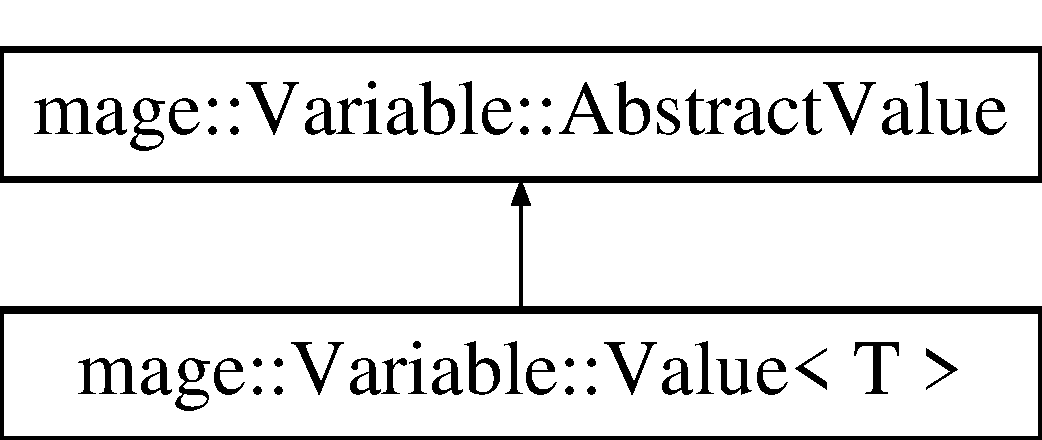
\includegraphics[height=2.000000cm]{structmage_1_1_variable_1_1_value}
\end{center}
\end{figure}
\subsection*{Public Member Functions}
\begin{DoxyCompactItemize}
\item 
\hyperlink{structmage_1_1_variable_1_1_value_a1e29cc5eaeb8356a11a1eca0232cf162}{Value} (const T $\ast$value)
\item 
virtual \hyperlink{structmage_1_1_variable_1_1_value_ab0b88d59c1049b89557fbaf649a3b459}{$\sim$\+Value} ()
\item 
virtual const void $\ast$ \hyperlink{structmage_1_1_variable_1_1_value_a04d70496ebb7ad71dafa3df877daeb26}{Get\+Value} () const override
\end{DoxyCompactItemize}
\subsection*{Private Attributes}
\begin{DoxyCompactItemize}
\item 
const T $\ast$ \hyperlink{structmage_1_1_variable_1_1_value_aa15243b8811b108a0c7bff05456e377c}{m\+\_\+value}
\end{DoxyCompactItemize}


\subsection{Detailed Description}
\subsubsection*{template$<$typename T$>$\newline
struct mage\+::\+Variable\+::\+Value$<$ T $>$}

A struct of immutable values. 
\begin{DoxyTemplParams}{Template Parameters}
{\em T} & The type of the value. \\
\hline
\end{DoxyTemplParams}


\subsection{Constructor \& Destructor Documentation}
\hypertarget{structmage_1_1_variable_1_1_value_a1e29cc5eaeb8356a11a1eca0232cf162}{}\label{structmage_1_1_variable_1_1_value_a1e29cc5eaeb8356a11a1eca0232cf162} 
\index{mage\+::\+Variable\+::\+Value@{mage\+::\+Variable\+::\+Value}!Value@{Value}}
\index{Value@{Value}!mage\+::\+Variable\+::\+Value@{mage\+::\+Variable\+::\+Value}}
\subsubsection{\texorpdfstring{Value()}{Value()}}
{\footnotesize\ttfamily template$<$typename T $>$ \\
\hyperlink{structmage_1_1_variable_1_1_value}{mage\+::\+Variable\+::\+Value}$<$ T $>$\+::\hyperlink{structmage_1_1_variable_1_1_value}{Value} (\begin{DoxyParamCaption}\item[{const T $\ast$}]{value }\end{DoxyParamCaption})}

Constructs a value.


\begin{DoxyParams}[1]{Parameters}
\mbox{\tt in}  & {\em value} & A pointer to the value. \\
\hline
\end{DoxyParams}
\hypertarget{structmage_1_1_variable_1_1_value_ab0b88d59c1049b89557fbaf649a3b459}{}\label{structmage_1_1_variable_1_1_value_ab0b88d59c1049b89557fbaf649a3b459} 
\index{mage\+::\+Variable\+::\+Value@{mage\+::\+Variable\+::\+Value}!````~Value@{$\sim$\+Value}}
\index{````~Value@{$\sim$\+Value}!mage\+::\+Variable\+::\+Value@{mage\+::\+Variable\+::\+Value}}
\subsubsection{\texorpdfstring{$\sim$\+Value()}{~Value()}}
{\footnotesize\ttfamily template$<$typename T $>$ \\
virtual \hyperlink{structmage_1_1_variable_1_1_value}{mage\+::\+Variable\+::\+Value}$<$ T $>$\+::$\sim$\hyperlink{structmage_1_1_variable_1_1_value}{Value} (\begin{DoxyParamCaption}{ }\end{DoxyParamCaption})\hspace{0.3cm}{\ttfamily [virtual]}}

Destructs this value. 

\subsection{Member Function Documentation}
\hypertarget{structmage_1_1_variable_1_1_value_a04d70496ebb7ad71dafa3df877daeb26}{}\label{structmage_1_1_variable_1_1_value_a04d70496ebb7ad71dafa3df877daeb26} 
\index{mage\+::\+Variable\+::\+Value@{mage\+::\+Variable\+::\+Value}!Get\+Value@{Get\+Value}}
\index{Get\+Value@{Get\+Value}!mage\+::\+Variable\+::\+Value@{mage\+::\+Variable\+::\+Value}}
\subsubsection{\texorpdfstring{Get\+Value()}{GetValue()}}
{\footnotesize\ttfamily template$<$typename T $>$ \\
virtual const void$\ast$ \hyperlink{structmage_1_1_variable_1_1_value}{mage\+::\+Variable\+::\+Value}$<$ T $>$\+::Get\+Value (\begin{DoxyParamCaption}{ }\end{DoxyParamCaption}) const\hspace{0.3cm}{\ttfamily [override]}, {\ttfamily [virtual]}}

Returns the value of this value.

\begin{DoxyReturn}{Returns}
A pointer to the value of this value. 
\end{DoxyReturn}


Implements \hyperlink{structmage_1_1_variable_1_1_abstract_value_aede2a77b571b80794a4254e34144f4c1}{mage\+::\+Variable\+::\+Abstract\+Value}.



\subsection{Member Data Documentation}
\hypertarget{structmage_1_1_variable_1_1_value_aa15243b8811b108a0c7bff05456e377c}{}\label{structmage_1_1_variable_1_1_value_aa15243b8811b108a0c7bff05456e377c} 
\index{mage\+::\+Variable\+::\+Value@{mage\+::\+Variable\+::\+Value}!m\+\_\+value@{m\+\_\+value}}
\index{m\+\_\+value@{m\+\_\+value}!mage\+::\+Variable\+::\+Value@{mage\+::\+Variable\+::\+Value}}
\subsubsection{\texorpdfstring{m\+\_\+value}{m\_value}}
{\footnotesize\ttfamily template$<$typename T $>$ \\
const T$\ast$ \hyperlink{structmage_1_1_variable_1_1_value}{mage\+::\+Variable\+::\+Value}$<$ T $>$\+::m\+\_\+value\hspace{0.3cm}{\ttfamily [private]}}

A pointer to the value of this value. 
\hypertarget{structmage_1_1_variable}{}\section{mage\+:\+:Variable Struct Reference}
\label{structmage_1_1_variable}\index{mage\+::\+Variable@{mage\+::\+Variable}}


{\ttfamily \#include $<$variable.\+hpp$>$}

\subsection*{Classes}
\begin{DoxyCompactItemize}
\item 
struct \hyperlink{structmage_1_1_variable_1_1_abstract_value}{Abstract\+Value}
\item 
struct \hyperlink{structmage_1_1_variable_1_1_value}{Value}
\end{DoxyCompactItemize}
\subsection*{Public Member Functions}
\begin{DoxyCompactItemize}
\item 
{\footnotesize template$<$typename T $>$ }\\\hyperlink{structmage_1_1_variable_a79e412d8882a5adc1d5c4ac8587ed7e8}{Variable} (const string \&name, const T $\ast$value)
\item 
\hyperlink{structmage_1_1_variable_a8f4d3e950b25b14e996ad074e42a5e9e}{$\sim$\+Variable} ()
\item 
const string \& \hyperlink{structmage_1_1_variable_a7f70fdadf34cdf6b26adc9910eade11d}{Get\+Name} () const
\item 
const void $\ast$ \hyperlink{structmage_1_1_variable_a65ecc95bcdc26733394d3a32d3d698f1}{Get\+Value} () const
\end{DoxyCompactItemize}
\subsection*{Private Attributes}
\begin{DoxyCompactItemize}
\item 
const string \hyperlink{structmage_1_1_variable_afac262aa51bb1dfe447d501abcaa08d0}{m\+\_\+name}
\item 
const \hyperlink{structmage_1_1_variable_1_1_abstract_value}{Abstract\+Value} $\ast$ \hyperlink{structmage_1_1_variable_a99388f3fbccf983b8d6954fd31d0eb27}{m\+\_\+value}
\end{DoxyCompactItemize}


\subsection{Detailed Description}
A struct of variables. 

\subsection{Constructor \& Destructor Documentation}
\hypertarget{structmage_1_1_variable_a79e412d8882a5adc1d5c4ac8587ed7e8}{}\label{structmage_1_1_variable_a79e412d8882a5adc1d5c4ac8587ed7e8} 
\index{mage\+::\+Variable@{mage\+::\+Variable}!Variable@{Variable}}
\index{Variable@{Variable}!mage\+::\+Variable@{mage\+::\+Variable}}
\subsubsection{\texorpdfstring{Variable()}{Variable()}}
{\footnotesize\ttfamily template$<$typename T $>$ \\
mage\+::\+Variable\+::\+Variable (\begin{DoxyParamCaption}\item[{const string \&}]{name,  }\item[{const T $\ast$}]{value }\end{DoxyParamCaption})}

Constructs a variable.


\begin{DoxyTemplParams}{Template Parameters}
{\em T} & The type of the value. \\
\hline
\end{DoxyTemplParams}

\begin{DoxyParams}[1]{Parameters}
\mbox{\tt in}  & {\em name} & The name. \\
\hline
\mbox{\tt in}  & {\em value} & A pointer to the value. \\
\hline
\end{DoxyParams}
\hypertarget{structmage_1_1_variable_a8f4d3e950b25b14e996ad074e42a5e9e}{}\label{structmage_1_1_variable_a8f4d3e950b25b14e996ad074e42a5e9e} 
\index{mage\+::\+Variable@{mage\+::\+Variable}!````~Variable@{$\sim$\+Variable}}
\index{````~Variable@{$\sim$\+Variable}!mage\+::\+Variable@{mage\+::\+Variable}}
\subsubsection{\texorpdfstring{$\sim$\+Variable()}{~Variable()}}
{\footnotesize\ttfamily mage\+::\+Variable\+::$\sim$\+Variable (\begin{DoxyParamCaption}{ }\end{DoxyParamCaption})}

Destructs this variable. 

\subsection{Member Function Documentation}
\hypertarget{structmage_1_1_variable_a7f70fdadf34cdf6b26adc9910eade11d}{}\label{structmage_1_1_variable_a7f70fdadf34cdf6b26adc9910eade11d} 
\index{mage\+::\+Variable@{mage\+::\+Variable}!Get\+Name@{Get\+Name}}
\index{Get\+Name@{Get\+Name}!mage\+::\+Variable@{mage\+::\+Variable}}
\subsubsection{\texorpdfstring{Get\+Name()}{GetName()}}
{\footnotesize\ttfamily const string\& mage\+::\+Variable\+::\+Get\+Name (\begin{DoxyParamCaption}{ }\end{DoxyParamCaption}) const}

Returns the name of this variable.

\begin{DoxyReturn}{Returns}
A reference to the name of this variable. 
\end{DoxyReturn}
\hypertarget{structmage_1_1_variable_a65ecc95bcdc26733394d3a32d3d698f1}{}\label{structmage_1_1_variable_a65ecc95bcdc26733394d3a32d3d698f1} 
\index{mage\+::\+Variable@{mage\+::\+Variable}!Get\+Value@{Get\+Value}}
\index{Get\+Value@{Get\+Value}!mage\+::\+Variable@{mage\+::\+Variable}}
\subsubsection{\texorpdfstring{Get\+Value()}{GetValue()}}
{\footnotesize\ttfamily const void$\ast$ mage\+::\+Variable\+::\+Get\+Value (\begin{DoxyParamCaption}{ }\end{DoxyParamCaption}) const}

Returns the value of this variable.

\begin{DoxyReturn}{Returns}
A pointer to the value of this variable. 
\end{DoxyReturn}


\subsection{Member Data Documentation}
\hypertarget{structmage_1_1_variable_afac262aa51bb1dfe447d501abcaa08d0}{}\label{structmage_1_1_variable_afac262aa51bb1dfe447d501abcaa08d0} 
\index{mage\+::\+Variable@{mage\+::\+Variable}!m\+\_\+name@{m\+\_\+name}}
\index{m\+\_\+name@{m\+\_\+name}!mage\+::\+Variable@{mage\+::\+Variable}}
\subsubsection{\texorpdfstring{m\+\_\+name}{m\_name}}
{\footnotesize\ttfamily const string mage\+::\+Variable\+::m\+\_\+name\hspace{0.3cm}{\ttfamily [private]}}

The name of this variable. \hypertarget{structmage_1_1_variable_a99388f3fbccf983b8d6954fd31d0eb27}{}\label{structmage_1_1_variable_a99388f3fbccf983b8d6954fd31d0eb27} 
\index{mage\+::\+Variable@{mage\+::\+Variable}!m\+\_\+value@{m\+\_\+value}}
\index{m\+\_\+value@{m\+\_\+value}!mage\+::\+Variable@{mage\+::\+Variable}}
\subsubsection{\texorpdfstring{m\+\_\+value}{m\_value}}
{\footnotesize\ttfamily const \hyperlink{structmage_1_1_variable_1_1_abstract_value}{Abstract\+Value}$\ast$ mage\+::\+Variable\+::m\+\_\+value\hspace{0.3cm}{\ttfamily [private]}}

A pointer to the value of this variable. 
\hypertarget{classmage_1_1_variable_script}{}\section{mage\+:\+:Variable\+Script Class Reference}
\label{classmage_1_1_variable_script}\index{mage\+::\+Variable\+Script@{mage\+::\+Variable\+Script}}


{\ttfamily \#include $<$variable\+\_\+script.\+hpp$>$}

Inheritance diagram for mage\+:\+:Variable\+Script\+:\begin{figure}[H]
\begin{center}
\leavevmode
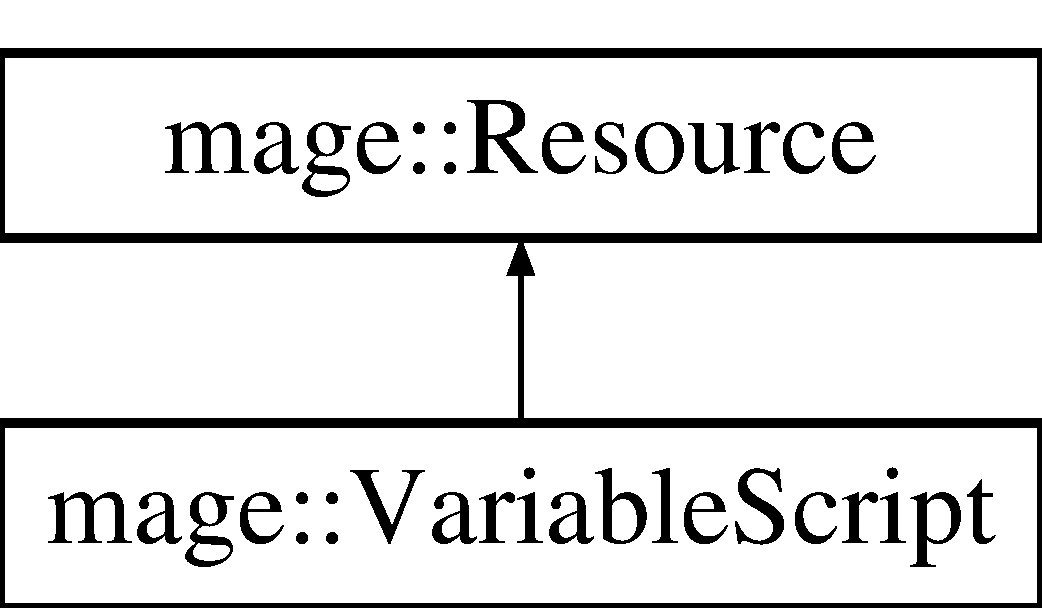
\includegraphics[height=2.000000cm]{classmage_1_1_variable_script}
\end{center}
\end{figure}
\subsection*{Public Member Functions}
\begin{DoxyCompactItemize}
\item 
\hyperlink{classmage_1_1_variable_script_a8b40c66f4f025bbf85b60ac57eb92248}{Variable\+Script} (const string \&name, const string \&path=\char`\"{}./\char`\"{})
\item 
virtual \hyperlink{classmage_1_1_variable_script_a8c488e779a6444559bded669a3e038c8}{$\sim$\+Variable\+Script} ()
\item 
void \hyperlink{classmage_1_1_variable_script_a24268eb0ad76b0ead392f341b55d641a}{Import\+Script} (const string \&filename=\char`\"{}\char`\"{})
\item 
void \hyperlink{classmage_1_1_variable_script_a863930f2c84786c2bb5bfa090cda06f7}{Export\+Script} (const string \&filename=\char`\"{}\char`\"{})
\item 
bool \hyperlink{classmage_1_1_variable_script_a8ae619cdc5519a753780360abab87430}{Is\+Empty} () const
\item 
size\+\_\+t \hyperlink{classmage_1_1_variable_script_a27ed94a510a3dab0e60b42b650ca6f09}{Get\+Nb\+Of\+Variables} () const
\item 
{\footnotesize template$<$typename T $>$ }\\void \hyperlink{classmage_1_1_variable_script_aa9a8bb9b6133ce853052820961320ca9}{Add\+Variable} (const string \&name, \hyperlink{namespacemage_a530428e73bac0ba7fe84b29086a9e33a}{Variable\+Type} type, const T $\ast$value)
\item 
void \hyperlink{classmage_1_1_variable_script_a4970ef4faafb1a6a43c4648ec9f36cce}{Remove\+Variable} (const string \&name)
\item 
{\footnotesize template$<$typename T $>$ }\\const T $\ast$ \hyperlink{classmage_1_1_variable_script_a231b83e1e32b882489ed90faa69f7137}{Get\+Value\+Of\+Variable} (const string \&name) const
\item 
{\footnotesize template$<$typename T $>$ }\\void \hyperlink{classmage_1_1_variable_script_a1b6daa6b226e43564408ab54e4c65eb7}{Set\+Value\+Of\+Variable} (const string \&name, const T $\ast$value)
\end{DoxyCompactItemize}
\subsection*{Protected Member Functions}
\begin{DoxyCompactItemize}
\item 
void \hyperlink{classmage_1_1_variable_script_ae7ab24f4d3bb11579ce9cfb690ba7a4f}{Import\+Variable} (const string \&name, F\+I\+LE $\ast$file)
\item 
void \hyperlink{classmage_1_1_variable_script_a69aaa511e7e00912cee95c04cf31b4f5}{Export\+Variable} (const \hyperlink{structmage_1_1_variable}{Variable} $\ast$variable, F\+I\+LE $\ast$file)
\end{DoxyCompactItemize}
\subsection*{Protected Attributes}
\begin{DoxyCompactItemize}
\item 
list$<$ \hyperlink{structmage_1_1_variable}{Variable} $\ast$$>$ \hyperlink{classmage_1_1_variable_script_a14dfd0518fe06cbfaf409fd5223f63e5}{m\+\_\+variables}
\end{DoxyCompactItemize}


\subsection{Detailed Description}
A class of variable scripts. 

\subsection{Constructor \& Destructor Documentation}
\hypertarget{classmage_1_1_variable_script_a8b40c66f4f025bbf85b60ac57eb92248}{}\label{classmage_1_1_variable_script_a8b40c66f4f025bbf85b60ac57eb92248} 
\index{mage\+::\+Variable\+Script@{mage\+::\+Variable\+Script}!Variable\+Script@{Variable\+Script}}
\index{Variable\+Script@{Variable\+Script}!mage\+::\+Variable\+Script@{mage\+::\+Variable\+Script}}
\subsubsection{\texorpdfstring{Variable\+Script()}{VariableScript()}}
{\footnotesize\ttfamily mage\+::\+Variable\+Script\+::\+Variable\+Script (\begin{DoxyParamCaption}\item[{const string \&}]{name,  }\item[{const string \&}]{path = {\ttfamily \char`\"{}./\char`\"{}} }\end{DoxyParamCaption})}

Constructs a variable script.


\begin{DoxyParams}[1]{Parameters}
\mbox{\tt in}  & {\em name} & A reference to the name of the variable script. \\
\hline
\mbox{\tt in}  & {\em path} & A reference to the path of the variable script. \\
\hline
\end{DoxyParams}
\hypertarget{classmage_1_1_variable_script_a8c488e779a6444559bded669a3e038c8}{}\label{classmage_1_1_variable_script_a8c488e779a6444559bded669a3e038c8} 
\index{mage\+::\+Variable\+Script@{mage\+::\+Variable\+Script}!````~Variable\+Script@{$\sim$\+Variable\+Script}}
\index{````~Variable\+Script@{$\sim$\+Variable\+Script}!mage\+::\+Variable\+Script@{mage\+::\+Variable\+Script}}
\subsubsection{\texorpdfstring{$\sim$\+Variable\+Script()}{~VariableScript()}}
{\footnotesize\ttfamily virtual mage\+::\+Variable\+Script\+::$\sim$\+Variable\+Script (\begin{DoxyParamCaption}{ }\end{DoxyParamCaption})\hspace{0.3cm}{\ttfamily [virtual]}}

Destruct this variable script. 

\subsection{Member Function Documentation}
\hypertarget{classmage_1_1_variable_script_aa9a8bb9b6133ce853052820961320ca9}{}\label{classmage_1_1_variable_script_aa9a8bb9b6133ce853052820961320ca9} 
\index{mage\+::\+Variable\+Script@{mage\+::\+Variable\+Script}!Add\+Variable@{Add\+Variable}}
\index{Add\+Variable@{Add\+Variable}!mage\+::\+Variable\+Script@{mage\+::\+Variable\+Script}}
\subsubsection{\texorpdfstring{Add\+Variable()}{AddVariable()}}
{\footnotesize\ttfamily template$<$typename T $>$ \\
void mage\+::\+Variable\+Script\+::\+Add\+Variable (\begin{DoxyParamCaption}\item[{const string \&}]{name,  }\item[{\hyperlink{namespacemage_a530428e73bac0ba7fe84b29086a9e33a}{Variable\+Type}}]{type,  }\item[{const T $\ast$}]{value }\end{DoxyParamCaption})}

Adds the given variable to this variable script.

\begin{DoxyPrecond}{Precondition}
No variable with the name {\itshape name} exists in this variable script. 
\end{DoxyPrecond}

\begin{DoxyTemplParams}{Template Parameters}
{\em T} & The type of the value. \\
\hline
\end{DoxyTemplParams}

\begin{DoxyParams}[1]{Parameters}
\mbox{\tt in}  & {\em name} & The name of the variable. \\
\hline
\mbox{\tt in}  & {\em type} & The type of the variable. \\
\hline
\mbox{\tt in}  & {\em value} & A pointer to the value of the variable. \\
\hline
\end{DoxyParams}
\hypertarget{classmage_1_1_variable_script_a863930f2c84786c2bb5bfa090cda06f7}{}\label{classmage_1_1_variable_script_a863930f2c84786c2bb5bfa090cda06f7} 
\index{mage\+::\+Variable\+Script@{mage\+::\+Variable\+Script}!Export\+Script@{Export\+Script}}
\index{Export\+Script@{Export\+Script}!mage\+::\+Variable\+Script@{mage\+::\+Variable\+Script}}
\subsubsection{\texorpdfstring{Export\+Script()}{ExportScript()}}
{\footnotesize\ttfamily void mage\+::\+Variable\+Script\+::\+Export\+Script (\begin{DoxyParamCaption}\item[{const string \&}]{filename = {\ttfamily \char`\"{}\char`\"{}} }\end{DoxyParamCaption})}

Exports this variable script to the file with the given filename.


\begin{DoxyParams}[1]{Parameters}
\mbox{\tt in}  & {\em filename} & A reference to the filename. \\
\hline
\end{DoxyParams}
\hypertarget{classmage_1_1_variable_script_a69aaa511e7e00912cee95c04cf31b4f5}{}\label{classmage_1_1_variable_script_a69aaa511e7e00912cee95c04cf31b4f5} 
\index{mage\+::\+Variable\+Script@{mage\+::\+Variable\+Script}!Export\+Variable@{Export\+Variable}}
\index{Export\+Variable@{Export\+Variable}!mage\+::\+Variable\+Script@{mage\+::\+Variable\+Script}}
\subsubsection{\texorpdfstring{Export\+Variable()}{ExportVariable()}}
{\footnotesize\ttfamily void mage\+::\+Variable\+Script\+::\+Export\+Variable (\begin{DoxyParamCaption}\item[{const \hyperlink{structmage_1_1_variable}{Variable} $\ast$}]{variable,  }\item[{F\+I\+LE $\ast$}]{file }\end{DoxyParamCaption})\hspace{0.3cm}{\ttfamily [protected]}}

Export the given variable from this variable script to the given file.


\begin{DoxyParams}[1]{Parameters}
\mbox{\tt in}  & {\em variable} & A pointer to the variable variable. \\
\hline
\mbox{\tt in}  & {\em file} & A pointer to a file used for exporting. \\
\hline
\end{DoxyParams}
\hypertarget{classmage_1_1_variable_script_a27ed94a510a3dab0e60b42b650ca6f09}{}\label{classmage_1_1_variable_script_a27ed94a510a3dab0e60b42b650ca6f09} 
\index{mage\+::\+Variable\+Script@{mage\+::\+Variable\+Script}!Get\+Nb\+Of\+Variables@{Get\+Nb\+Of\+Variables}}
\index{Get\+Nb\+Of\+Variables@{Get\+Nb\+Of\+Variables}!mage\+::\+Variable\+Script@{mage\+::\+Variable\+Script}}
\subsubsection{\texorpdfstring{Get\+Nb\+Of\+Variables()}{GetNbOfVariables()}}
{\footnotesize\ttfamily size\+\_\+t mage\+::\+Variable\+Script\+::\+Get\+Nb\+Of\+Variables (\begin{DoxyParamCaption}{ }\end{DoxyParamCaption}) const}

Returns the number of variables in this variable script.

\begin{DoxyReturn}{Returns}
The number of variables in this variable script. 
\end{DoxyReturn}
\hypertarget{classmage_1_1_variable_script_a231b83e1e32b882489ed90faa69f7137}{}\label{classmage_1_1_variable_script_a231b83e1e32b882489ed90faa69f7137} 
\index{mage\+::\+Variable\+Script@{mage\+::\+Variable\+Script}!Get\+Value\+Of\+Variable@{Get\+Value\+Of\+Variable}}
\index{Get\+Value\+Of\+Variable@{Get\+Value\+Of\+Variable}!mage\+::\+Variable\+Script@{mage\+::\+Variable\+Script}}
\subsubsection{\texorpdfstring{Get\+Value\+Of\+Variable()}{GetValueOfVariable()}}
{\footnotesize\ttfamily template$<$typename T $>$ \\
const T$\ast$ mage\+::\+Variable\+Script\+::\+Get\+Value\+Of\+Variable (\begin{DoxyParamCaption}\item[{const string \&}]{name }\end{DoxyParamCaption}) const}

Returns the value of the given variable in this variable script.


\begin{DoxyTemplParams}{Template Parameters}
{\em T} & The type of the value. \\
\hline
\end{DoxyTemplParams}

\begin{DoxyParams}[1]{Parameters}
\mbox{\tt in}  & {\em name} & The name of the variable. \\
\hline
\end{DoxyParams}
\begin{DoxyReturn}{Returns}
{\ttfamily nullptr} if no variable with the name {\itshape name} exists in this variable script. 

A pointer to the value of the variable. 
\end{DoxyReturn}
\hypertarget{classmage_1_1_variable_script_a24268eb0ad76b0ead392f341b55d641a}{}\label{classmage_1_1_variable_script_a24268eb0ad76b0ead392f341b55d641a} 
\index{mage\+::\+Variable\+Script@{mage\+::\+Variable\+Script}!Import\+Script@{Import\+Script}}
\index{Import\+Script@{Import\+Script}!mage\+::\+Variable\+Script@{mage\+::\+Variable\+Script}}
\subsubsection{\texorpdfstring{Import\+Script()}{ImportScript()}}
{\footnotesize\ttfamily void mage\+::\+Variable\+Script\+::\+Import\+Script (\begin{DoxyParamCaption}\item[{const string \&}]{filename = {\ttfamily \char`\"{}\char`\"{}} }\end{DoxyParamCaption})}

Imports this variable script from its associated file.


\begin{DoxyParams}[1]{Parameters}
\mbox{\tt in}  & {\em filename} & A reference to the filename. \\
\hline
\end{DoxyParams}
\hypertarget{classmage_1_1_variable_script_ae7ab24f4d3bb11579ce9cfb690ba7a4f}{}\label{classmage_1_1_variable_script_ae7ab24f4d3bb11579ce9cfb690ba7a4f} 
\index{mage\+::\+Variable\+Script@{mage\+::\+Variable\+Script}!Import\+Variable@{Import\+Variable}}
\index{Import\+Variable@{Import\+Variable}!mage\+::\+Variable\+Script@{mage\+::\+Variable\+Script}}
\subsubsection{\texorpdfstring{Import\+Variable()}{ImportVariable()}}
{\footnotesize\ttfamily void mage\+::\+Variable\+Script\+::\+Import\+Variable (\begin{DoxyParamCaption}\item[{const string \&}]{name,  }\item[{F\+I\+LE $\ast$}]{file }\end{DoxyParamCaption})\hspace{0.3cm}{\ttfamily [protected]}}

Import the given variable from the given file to this variable script.

\begin{DoxyPrecond}{Precondition}
No variable with the name {\itshape name} exists in this variable script. 
\end{DoxyPrecond}

\begin{DoxyParams}[1]{Parameters}
\mbox{\tt in}  & {\em name} & The name of the variable. \\
\hline
\mbox{\tt in}  & {\em file} & A pointer to a file used for importing. \\
\hline
\end{DoxyParams}
\hypertarget{classmage_1_1_variable_script_a8ae619cdc5519a753780360abab87430}{}\label{classmage_1_1_variable_script_a8ae619cdc5519a753780360abab87430} 
\index{mage\+::\+Variable\+Script@{mage\+::\+Variable\+Script}!Is\+Empty@{Is\+Empty}}
\index{Is\+Empty@{Is\+Empty}!mage\+::\+Variable\+Script@{mage\+::\+Variable\+Script}}
\subsubsection{\texorpdfstring{Is\+Empty()}{IsEmpty()}}
{\footnotesize\ttfamily bool mage\+::\+Variable\+Script\+::\+Is\+Empty (\begin{DoxyParamCaption}{ }\end{DoxyParamCaption}) const}

Checks wether this variable script is empty.

\begin{DoxyReturn}{Returns}
{\ttfamily true} if this variable script is empty. {\ttfamily false} otherwise. 
\end{DoxyReturn}
\hypertarget{classmage_1_1_variable_script_a4970ef4faafb1a6a43c4648ec9f36cce}{}\label{classmage_1_1_variable_script_a4970ef4faafb1a6a43c4648ec9f36cce} 
\index{mage\+::\+Variable\+Script@{mage\+::\+Variable\+Script}!Remove\+Variable@{Remove\+Variable}}
\index{Remove\+Variable@{Remove\+Variable}!mage\+::\+Variable\+Script@{mage\+::\+Variable\+Script}}
\subsubsection{\texorpdfstring{Remove\+Variable()}{RemoveVariable()}}
{\footnotesize\ttfamily void mage\+::\+Variable\+Script\+::\+Remove\+Variable (\begin{DoxyParamCaption}\item[{const string \&}]{name }\end{DoxyParamCaption})}

Removes the given variable from this variable script.


\begin{DoxyParams}[1]{Parameters}
\mbox{\tt in}  & {\em name} & The name of the variable. \\
\hline
\end{DoxyParams}
\hypertarget{classmage_1_1_variable_script_a1b6daa6b226e43564408ab54e4c65eb7}{}\label{classmage_1_1_variable_script_a1b6daa6b226e43564408ab54e4c65eb7} 
\index{mage\+::\+Variable\+Script@{mage\+::\+Variable\+Script}!Set\+Value\+Of\+Variable@{Set\+Value\+Of\+Variable}}
\index{Set\+Value\+Of\+Variable@{Set\+Value\+Of\+Variable}!mage\+::\+Variable\+Script@{mage\+::\+Variable\+Script}}
\subsubsection{\texorpdfstring{Set\+Value\+Of\+Variable()}{SetValueOfVariable()}}
{\footnotesize\ttfamily template$<$typename T $>$ \\
void mage\+::\+Variable\+Script\+::\+Set\+Value\+Of\+Variable (\begin{DoxyParamCaption}\item[{const string \&}]{name,  }\item[{const T $\ast$}]{value }\end{DoxyParamCaption})}

Sets the value of the given variable in this variable script.


\begin{DoxyTemplParams}{Template Parameters}
{\em T} & The type of the value. \\
\hline
\end{DoxyTemplParams}

\begin{DoxyParams}[1]{Parameters}
\mbox{\tt in}  & {\em name} & The name of the variable. \\
\hline
\mbox{\tt in}  & {\em value} & A pointer to the value of the variable. \\
\hline
\end{DoxyParams}
\begin{DoxyNote}{Note}
Nothing happens if no variable with the name {\itshape name} exists in this variable script. 
\end{DoxyNote}


\subsection{Member Data Documentation}
\hypertarget{classmage_1_1_variable_script_a14dfd0518fe06cbfaf409fd5223f63e5}{}\label{classmage_1_1_variable_script_a14dfd0518fe06cbfaf409fd5223f63e5} 
\index{mage\+::\+Variable\+Script@{mage\+::\+Variable\+Script}!m\+\_\+variables@{m\+\_\+variables}}
\index{m\+\_\+variables@{m\+\_\+variables}!mage\+::\+Variable\+Script@{mage\+::\+Variable\+Script}}
\subsubsection{\texorpdfstring{m\+\_\+variables}{m\_variables}}
{\footnotesize\ttfamily list$<$ \hyperlink{structmage_1_1_variable}{Variable} $\ast$ $>$ mage\+::\+Variable\+Script\+::m\+\_\+variables\hspace{0.3cm}{\ttfamily [protected]}}

Linked list containing the variables in this variable script. 
\hypertarget{structmage_1_1_vertex}{}\section{mage\+:\+:Vertex Struct Reference}
\label{structmage_1_1_vertex}\index{mage\+::\+Vertex@{mage\+::\+Vertex}}


{\ttfamily \#include $<$vertex.\+hpp$>$}

\subsection*{Public Member Functions}
\begin{DoxyCompactItemize}
\item 
\hyperlink{structmage_1_1_vertex_a8bf3578fcb5595eab057dc2d1f916dce}{Vertex} ()
\item 
\hyperlink{structmage_1_1_vertex_a19ef5e9829752aa2134bc25617ce910d}{Vertex} (X\+M\+F\+L\+O\+A\+T3 \hyperlink{structmage_1_1_vertex_a9d726a508934b3baccfb01ea912420e7}{p}, X\+M\+F\+L\+O\+A\+T3 \hyperlink{structmage_1_1_vertex_a0b6c65dd92ba473f490e790189d92daf}{n}, X\+M\+F\+L\+O\+A\+T2 \hyperlink{structmage_1_1_vertex_a85ae82408f02d64ae567a74efe151188}{tex})
\end{DoxyCompactItemize}
\subsection*{Public Attributes}
\begin{DoxyCompactItemize}
\item 
X\+M\+F\+L\+O\+A\+T3 \hyperlink{structmage_1_1_vertex_a9d726a508934b3baccfb01ea912420e7}{p}
\item 
X\+M\+F\+L\+O\+A\+T3 \hyperlink{structmage_1_1_vertex_a0b6c65dd92ba473f490e790189d92daf}{n}
\item 
X\+M\+F\+L\+O\+A\+T2 \hyperlink{structmage_1_1_vertex_a85ae82408f02d64ae567a74efe151188}{tex}
\end{DoxyCompactItemize}


\subsection{Detailed Description}
A struct of vertices. 

\subsection{Constructor \& Destructor Documentation}
\hypertarget{structmage_1_1_vertex_a8bf3578fcb5595eab057dc2d1f916dce}{}\label{structmage_1_1_vertex_a8bf3578fcb5595eab057dc2d1f916dce} 
\index{mage\+::\+Vertex@{mage\+::\+Vertex}!Vertex@{Vertex}}
\index{Vertex@{Vertex}!mage\+::\+Vertex@{mage\+::\+Vertex}}
\subsubsection{\texorpdfstring{Vertex()}{Vertex()}\hspace{0.1cm}{\footnotesize\ttfamily [1/2]}}
{\footnotesize\ttfamily mage\+::\+Vertex\+::\+Vertex (\begin{DoxyParamCaption}{ }\end{DoxyParamCaption})}

Constructs a vertex. \hypertarget{structmage_1_1_vertex_a19ef5e9829752aa2134bc25617ce910d}{}\label{structmage_1_1_vertex_a19ef5e9829752aa2134bc25617ce910d} 
\index{mage\+::\+Vertex@{mage\+::\+Vertex}!Vertex@{Vertex}}
\index{Vertex@{Vertex}!mage\+::\+Vertex@{mage\+::\+Vertex}}
\subsubsection{\texorpdfstring{Vertex()}{Vertex()}\hspace{0.1cm}{\footnotesize\ttfamily [2/2]}}
{\footnotesize\ttfamily mage\+::\+Vertex\+::\+Vertex (\begin{DoxyParamCaption}\item[{X\+M\+F\+L\+O\+A\+T3}]{p,  }\item[{X\+M\+F\+L\+O\+A\+T3}]{n,  }\item[{X\+M\+F\+L\+O\+A\+T2}]{tex }\end{DoxyParamCaption})}

Constructs a vertex.

\begin{DoxyPrecond}{Precondition}
The length (L2-\/norm) of the normal must be equal to one (i.\+e. the normal vector is normalized). 
\end{DoxyPrecond}

\begin{DoxyParams}[1]{Parameters}
\mbox{\tt in}  & {\em p} & The position of the vertex (in object space). \\
\hline
\mbox{\tt in}  & {\em n} & The normal of the vertex. \\
\hline
\mbox{\tt in}  & {\em tex} & The texture coordinates of the vertex. \\
\hline
\end{DoxyParams}


\subsection{Member Data Documentation}
\hypertarget{structmage_1_1_vertex_a0b6c65dd92ba473f490e790189d92daf}{}\label{structmage_1_1_vertex_a0b6c65dd92ba473f490e790189d92daf} 
\index{mage\+::\+Vertex@{mage\+::\+Vertex}!n@{n}}
\index{n@{n}!mage\+::\+Vertex@{mage\+::\+Vertex}}
\subsubsection{\texorpdfstring{n}{n}}
{\footnotesize\ttfamily X\+M\+F\+L\+O\+A\+T3 mage\+::\+Vertex\+::n}

The normal of this vertex. \hypertarget{structmage_1_1_vertex_a9d726a508934b3baccfb01ea912420e7}{}\label{structmage_1_1_vertex_a9d726a508934b3baccfb01ea912420e7} 
\index{mage\+::\+Vertex@{mage\+::\+Vertex}!p@{p}}
\index{p@{p}!mage\+::\+Vertex@{mage\+::\+Vertex}}
\subsubsection{\texorpdfstring{p}{p}}
{\footnotesize\ttfamily X\+M\+F\+L\+O\+A\+T3 mage\+::\+Vertex\+::p}

The position of this vertex (in object space). \hypertarget{structmage_1_1_vertex_a85ae82408f02d64ae567a74efe151188}{}\label{structmage_1_1_vertex_a85ae82408f02d64ae567a74efe151188} 
\index{mage\+::\+Vertex@{mage\+::\+Vertex}!tex@{tex}}
\index{tex@{tex}!mage\+::\+Vertex@{mage\+::\+Vertex}}
\subsubsection{\texorpdfstring{tex}{tex}}
{\footnotesize\ttfamily X\+M\+F\+L\+O\+A\+T2 mage\+::\+Vertex\+::tex}

The texture coordinates of this vertex. 
\hypertarget{structmage_1_1_viewer_setup}{}\section{mage\+:\+:Viewer\+Setup Struct Reference}
\label{structmage_1_1_viewer_setup}\index{mage\+::\+Viewer\+Setup@{mage\+::\+Viewer\+Setup}}


{\ttfamily \#include $<$state.\+hpp$>$}

\subsection*{Public Member Functions}
\begin{DoxyCompactItemize}
\item 
\hyperlink{structmage_1_1_viewer_setup_a41acbd3bd1b8df2e175a57ee9bd07bda}{Viewer\+Setup} ()
\end{DoxyCompactItemize}
\subsection*{Public Attributes}
\begin{DoxyCompactItemize}
\item 
uint64\+\_\+t \hyperlink{structmage_1_1_viewer_setup_aed7b78b5437c46627949142f628c331d}{m\+\_\+view\+\_\+clear\+\_\+flags}
\end{DoxyCompactItemize}


\subsection{Detailed Description}
A struct of viewer setups. 

\subsection{Constructor \& Destructor Documentation}
\hypertarget{structmage_1_1_viewer_setup_a41acbd3bd1b8df2e175a57ee9bd07bda}{}\label{structmage_1_1_viewer_setup_a41acbd3bd1b8df2e175a57ee9bd07bda} 
\index{mage\+::\+Viewer\+Setup@{mage\+::\+Viewer\+Setup}!Viewer\+Setup@{Viewer\+Setup}}
\index{Viewer\+Setup@{Viewer\+Setup}!mage\+::\+Viewer\+Setup@{mage\+::\+Viewer\+Setup}}
\subsubsection{\texorpdfstring{Viewer\+Setup()}{ViewerSetup()}}
{\footnotesize\ttfamily mage\+::\+Viewer\+Setup\+::\+Viewer\+Setup (\begin{DoxyParamCaption}{ }\end{DoxyParamCaption})}

Constructs a viewer setup. 

\subsection{Member Data Documentation}
\hypertarget{structmage_1_1_viewer_setup_aed7b78b5437c46627949142f628c331d}{}\label{structmage_1_1_viewer_setup_aed7b78b5437c46627949142f628c331d} 
\index{mage\+::\+Viewer\+Setup@{mage\+::\+Viewer\+Setup}!m\+\_\+view\+\_\+clear\+\_\+flags@{m\+\_\+view\+\_\+clear\+\_\+flags}}
\index{m\+\_\+view\+\_\+clear\+\_\+flags@{m\+\_\+view\+\_\+clear\+\_\+flags}!mage\+::\+Viewer\+Setup@{mage\+::\+Viewer\+Setup}}
\subsubsection{\texorpdfstring{m\+\_\+view\+\_\+clear\+\_\+flags}{m\_view\_clear\_flags}}
{\footnotesize\ttfamily uint64\+\_\+t mage\+::\+Viewer\+Setup\+::m\+\_\+view\+\_\+clear\+\_\+flags}

Flags used for clearing the view. 
%--- End generated contents ---

% Index
\backmatter
\newpage
\phantomsection
\clearemptydoublepage
\addcontentsline{toc}{chapter}{Index}
\printindex

\end{document}
